% ============================================================
% main.tex —— 全书装配（Lead 独占）
% 编译：xelatex ×2，cwd = work/src，TMP = ../tmp
% ============================================================
\documentclass[11pt,fontset=none,openany,oneside]{ctexbook}
% ============================================================
% preamble.tex —— 导言区（Lead 独占维护；译者只读，不得修改）
% 编译：xelatex ×2，必须先把 TMP/TEMP 指到 work/tmp
% ============================================================
\usepackage[a4paper,top=2.6cm,bottom=2.6cm,left=2.6cm,right=2.6cm]{geometry}
\usepackage{amsmath,amssymb,amsthm,mathtools}
\usepackage{graphicx}
\usepackage{xcolor}
\usepackage{tikz}
\usepackage{enumitem}
\usepackage{array,booktabs,longtable,multirow,tabularx}
\usepackage{fancyhdr}
\usepackage[colorlinks=true,linkcolor=blue!55!black,citecolor=blue!55!black,urlcolor=blue!55!black]{hyperref}

% ---------- 字体（fontset=none + 显式文件；不要用 fontconfig） ----------
\setCJKmainfont[Path=C:/Windows/Fonts/,BoldFont=simhei.ttf,ItalicFont=simkai.ttf]{simsun.ttc}
\setCJKsansfont[Path=C:/Windows/Fonts/]{simhei.ttf}
\setCJKmonofont[Path=C:/Windows/Fonts/]{simfang.ttf}

% ---------- 排版细节 ----------
\linespread{1.15}
\setlength{\emergencystretch}{3em}
\setcounter{tocdepth}{2}
\setcounter{secnumdepth}{3}
\renewcommand{\proofname}{证明}
\newenvironment{proofof}[1]{\begin{proof}[#1]}{\end{proof}}

% 书签里禁止数学（防 hyperref 警告）：不把数学写进 \chapter/\section 标题即可

% ---------- 定理类环境（编号一律手工给定：\begin{theorem}[1.1]） ----------
\theoremstyle{plain}
\newtheorem*{theorem}{定理}
\newtheorem*{proposition}{命题}
\newtheorem*{lemma}{引理}
\newtheorem*{corollary}{推论}
\newtheorem*{claim}{断言}
\newtheorem*{fact}{事实}
\newtheorem*{conjecture}{猜想}
\newtheorem*{hypothesis}{假设}
\theoremstyle{definition}
\newtheorem*{definition}{定义}
\newtheorem*{example}{例}
\newtheorem*{exercise}{习题}
\newtheorem*{construction}{构造}
\newtheorem*{setup}{设定}
\newtheorem*{algorithm}{算法}
\newtheorem*{convention}{约定}
\newtheorem*{notation}{记号}
\newtheorem*{question}{问题}
\newtheorem*{problem}{问题}
\theoremstyle{remark}
\newtheorem*{remark}{注}
\newtheorem*{warning}{警告}

% ---------- 数学宏（全局统一；译者不得自造 \newcommand） ----------
\newcommand{\R}{\mathbb{R}}
\newcommand{\C}{\mathbb{C}}
\newcommand{\Z}{\mathbb{Z}}
\newcommand{\Q}{\mathbb{Q}}
\newcommand{\N}{\mathbb{N}}
\newcommand{\PP}{\mathbb{P}}
\newcommand{\HH}{\mathbb{H}}
\newcommand{\DD}{\mathbb{D}}
\newcommand{\OO}{\mathcal{O}}
\newcommand{\g}{\mathfrak{g}}
\newcommand{\h}{\mathfrak{h}}
\newcommand{\n}{\mathfrak{n}}
\renewcommand{\sl}{\mathfrak{sl}}
\newcommand{\gl}{\mathfrak{gl}}
\newcommand{\so}{\mathfrak{so}}
\newcommand{\su}{\mathfrak{su}}
\renewcommand{\sp}{\mathfrak{sp}}
\newcommand{\Tr}{\operatorname{Tr}}
\newcommand{\tr}{\operatorname{tr}}
\newcommand{\rank}{\operatorname{rank}}
\newcommand{\diag}{\operatorname{diag}}
\newcommand{\Spec}{\operatorname{Spec}}
\newcommand{\Hom}{\operatorname{Hom}}
\newcommand{\End}{\operatorname{End}}
\newcommand{\Aut}{\operatorname{Aut}}
\newcommand{\GL}{\operatorname{GL}}
\newcommand{\SL}{\operatorname{SL}}
\newcommand{\PSL}{\operatorname{PSL}}
\newcommand{\PGL}{\operatorname{PGL}}
\newcommand{\SO}{\operatorname{SO}}
\newcommand{\SU}{\operatorname{SU}}
\newcommand{\U}{\operatorname{U}}
\newcommand{\Mat}{\operatorname{Mat}}
\newcommand{\Rep}{\operatorname{Rep}}
\newcommand{\Loc}{\operatorname{Loc}}
\newcommand{\Fib}{\operatorname{Fib}}
\newcommand{\Iso}{\operatorname{Iso}}
\newcommand{\im}{\operatorname{im}}
\newcommand{\coker}{\operatorname{coker}}
\newcommand{\sgn}{\operatorname{sgn}}
\newcommand{\const}{\operatorname{const}}
\newcommand{\de}{\mathrm{d}}          % 微分 d（正体）
\newcommand{\ee}{\mathrm{e}}
\newcommand{\ii}{\mathrm{i}}
\newcommand{\dd}{\mathrm{d}}
\newcommand{\vol}{\operatorname{vol}}
\newcommand{\area}{\operatorname{area}}
\newcommand{\length}{\operatorname{length}}
\newcommand{\op}[1]{\operatorname{#1}}
\newcommand{\Sp}{\operatorname{Sp}}
\newcommand{\Stab}{\operatorname{Stab}}
\newcommand{\Sym}{\operatorname{Sym}}
\newcommand{\Homeo}{\operatorname{Homeo}}
\newcommand{\tq}{\text{；}}           % 数学环境里的中文分号（需自己包 \text{}）

% ---------- 插图（Lead 已裁好图；译者只引用，不得自造） ----------
% 用法：\Fig[0.75\linewidth]{figures/fig_1_3.png}{1.3}{中文图注}
\newcommand{\Fig}[4][0.75\linewidth]{%
  \begin{figure}[htbp]\centering
    \includegraphics[width=#1]{#2}\par\vspace{3pt}
    {\small 图~#3\quad #4}
  \end{figure}}
\newcommand{\FigNoNum}[3][0.75\linewidth]{%
  \begin{figure}[htbp]\centering
    \includegraphics[width=#1]{#2}\par\vspace{3pt}
    {\small #3}
  \end{figure}}

% ---------- 表格：按原文重排（不造新表） ----------
\renewcommand{\arraystretch}{1.15}

% ---------- 章首摘要（Springer 体例每章有 Abstract） ----------
\newcommand{\ChapterAbstract}[1]{\begin{quote}\small\noindent\textbf{摘要}\quad #1\end{quote}}
% ---------- 定理头格式：去掉 amsthm 自动加的 ASCII 括号 ----------
% 目标：\begin{theorem}[6.3] → 「定理 6.3」；\begin{theorem}[7.2（庞加莱单值化）] → 「定理 7.2（庞加莱单值化）」
\makeatletter
\renewcommand{\thmhead}[3]{\thmname{#1}\thmnumber{ #2}\thmnote{ #3}}
\makeatother
% ---------- 追加环境与宏（2026-11-03 第二批） ----------
\newcommand{\Lag}{\operatorname{Lag}}
\newcommand{\Conf}{\operatorname{Conf}}\newcommand{\PSU}{\operatorname{PSU}}
\newcommand{\USp}{\operatorname{USp}}
\newcommand{\PU}{\operatorname{PU}}
\newcommand{\Spin}{\operatorname{Spin}}
\newcommand{\Pin}{\operatorname{Pin}}


\begin{document}

\frontmatter
% 标题页（Lead 独占）
\begin{titlepage}
\centering
\vspace*{2.2cm}

{\LARGE\bfseries 谱网络\par}
\vspace{0.8cm}
{\Large\bfseries 连接高阶泰希米勒理论与 BPS 态\par}
\vspace{1.2cm}
{\large\textit{Spectral Networks}\par}
{\large\textit{Bridging higher-rank Teichmüller theory and BPS states}\par}

\vspace{2.4cm}
{\large
Clarence Kineider\\[2pt]
Georgios Kydonakis\\[2pt]
Eugen Rogozinnikov\\[2pt]
Valdo Tatitscheff\\[2pt]
Alexander Thomas\par}

\vspace{2.2cm}
{\large 中\;文\;译\;注\;本\par}
\vspace{0.5cm}
{\normalsize 底本：Springer Lecture Notes in Mathematics 2386\par}
{\normalsize arXiv:2412.03588v3 [math-ph]\par}

\vfill
{\small 译注与排版：DeepSeek Harness Agent（Lead + 8 名译者协作）\par}
{\small 2026 年 11 月\par}
\end{titlepage}


\tableofcontents

\IfFileExists{part/front.tex}{% ============================================================
% front.tex —— 前置部分：内容简介、前言、符号表
% 底本：LNM 2386
%   · 内容简介：PDF p2
%   · 前言（含致谢）：PDF p3–p6（印刷 v–viii）
%   · 符号表：PDF p15–p18（印刷 xvii–xx）
% 不译 Contents（PDF p7–13）
% ============================================================

% [原文 p.2]
\chapter*{内容简介}
\addcontentsline{toc}{chapter}{内容简介}

本书从统一的视角全面介绍谱网络，架起几何与超对称规范理论物理之间的桥梁。它提供了进入这一迅速发展领域前沿所需的基础背景，并平行处理几何与物理两个方面。在综述代数与几何中的基本主题之后，书中展开对高阶泰希米勒理论的详细介绍，包括用于 Hitchin 表示的 Fock–Goncharov 理论、极大表示以及较新的 $\Theta$ 正性概念。随后引入谱网络，强调它们借助所定义的非阿贝尔化与阿贝尔化映射在研究特征簇方面的效用。与此同时，书中探讨具有八个超荷的四维规范动力学的要点，包括电磁对偶、Seiberg–Witten 理论与 S 类理论。接着考察谱网络作为确定与分析 S 类理论中 BPS 谱之框架的作用。最后一章概述谱网络在一系列当代研究领域中的近期应用。本书面向希望进入该领域的研究人员与高年级学生，无论其背景是数学还是物理。

% [Tutor Note: 原文「eight supercharges」（八个超荷）即四维 $\mathcal N=2$ 超对称（每个超对称荷为四分量 Majorana 旋量，共 8 个超荷）；本书正文一律用花体 $\mathcal N$ 表示超对称的数目，勿与符号表中花体 $\mathcal N$ 的「量子场论中超对称的数目」混为一谈。]

% [原文 p.3（印刷 p.v）]
\chapter*{前言}
\addcontentsline{toc}{chapter}{前言}

谱网络由 Davide Gaiotto、Gregory W. Moore 与 Andrew Neitzke 在同名文章（2013 年发表于《\textit{Annales Henri Poincaré}》）中引入。它们是曲面上轨道的网络，自然出现在各种四维 $\mathcal N=2$ 量子场论的研究中，并提供一种特别有效的计算 BPS 谱的方法。从纯几何的观点看，它们给出黎曼曲面上的平坦联络与该曲面的一个谱覆盖上的平坦阿贝尔联络之间的一个新映射。同时，这些轨道网络给出平坦联络模空间上的局部坐标系，这些坐标系对于研究 Vladimir V. Fock 与 Alexander B. Goncharov 意义下的高阶泰希米勒空间很有价值。

自引入以来，谱网络不断证明自己是几何与数学物理中的一个深刻工具，其应用、推广以及与其他概念的联系与日俱增。然而，据我们所知，书本文献中仍缺少对该主题标准的、既严谨又具阐述性的综述；我们认为这主要是因为研究它们需要相当多样的背景。受我们各自多样研究兴趣的驱动，我们力求写出一本书：它既汇集了受过训练的数理学家与物理学家为严格入门该主题所需的必要基础，同时又展示了大量几何与数学物理中的应用，并以当前研究为指向。

本书旨在作为该主题的入门教材，以统一的方式从几何与数学物理的视角呈现谱网络及其众多应用。我们并不试图把这两种进路分开处理，而是提供宽广的动机与必要的背景，以抵达这一快速发展研究领域的前沿，同时解释相关的几何与物理方面。目标读者是希望进入该领域、具有数学或物理背景的研究人员与高年级学生。我们力求使这些几何与物理方面之间的联系更加透明，方法是在本书各节中有机地连接各个主题。鉴于谱网络的跨学科性质，我们尽力把书中所讨论的各个主题尽可能地统一起来。这种做法也特别解释了我们在同一卷书中同时使用标准数学术语与物理术语的决定。

% [原文 p.4（印刷 p.vi）]
谱网络及其在几何与数学物理中的应用是一个蓬勃发展的现代主题，当前正经历迅速的发展与扩张。因此，这一领域在工作中的数学家或物理学家看来，其面貌可能仍会发生变化。鉴于这种情况，我们选择以清晰的方式呈现理论的基本方面与迄今最坚实的应用。同时，我们收集了一系列当前研究发展的较广泛主题，在书的末尾以较为不严谨的方式呈现。这些方向上的重大进展可能使相关的进阶概念在未来以某种形式经历修订。

在正文之前的导论部分，我们提供一个历史概述，回顾高能物理、几何、特别是泰希米勒理论中的关键思想——正是它们导致谱网络作为计算具有两个或八个超对称的四维规范理论中 BPS 谱的工具被引入，以及它们在高等泰希米勒空间背景下的应用。虽然这部分并非作为这些主题的教学式导引而写——已有许多优秀的导引——但我们力求使尚不熟悉该领域的读者也能读懂并乐在其中，从而人人都能吸收关键概念，并从这一阐述中受益以理解本书后续各章。此处出现的一些重要数学概念会在后面各节中得到严谨而有教学意义的定义；我们在可能时强调这些联系。第 I 部分与第 II 部分完全独立于这一导论性论述，专注于几何中的各种主题。谱网络及其在几何中的用途在第 III 部分引入，而在第 IV 部分则从超对称规范理论的角度引入。

进一步展开本书的内容：第 I 部分是讨论谱网络所需数学背景的严谨而平实的入门。这里所包含的并非所有概念都在学术数学或物理课程中得到系统而充分的探讨，然而关于相关主题已有多种标准阐述；因此这一部分旨在为读者（无论其背景如何）建立共同的基础。对于已经熟悉所涉主题及其语言的读者，这一部分可以安全跳过。

第 II 部分是本书的核心部分之一，严谨地描述本书所讨论的高阶泰希米勒理论的多种主题。特别地，我们通过 Olivier Guichard 与 Anna Wienhard 引入的 $\Theta$ 正性这一核心概念，把高阶泰希米勒理论作为经典泰希米勒理论的高阶推广给出统一处理。此外，我们一方面讨论与泰希米勒空间上的 Thurston 剪切坐标的类比，另一方面讨论高阶泰希米勒空间上的 Fock–Goncharov 坐标。

% [原文 p.5（印刷 p.vii）]
谱网络在本书第 III 部分被明确定义。随后我们呈现并讨论谱网络在几何中最突出的应用：非阿贝尔化与阿贝尔化，它们把基础曲面的高阶泰希米勒空间与某个分歧覆盖——谱曲线——的阿贝尔特征簇联系起来。阿贝尔化的一种更解析的进路由精确 WKB 方法给出。从这个角度看，谱网络表现为 Borel 求和的 Stokes 图。Fock–Goncharov 坐标可以（至少在低秩时）由显式的单值数据恢复。

第 IV 部分探讨谱网络在具有 $\mathcal N=2$ 超对称的四维规范理论、特别是 S 类理论中的作用，将其作为描述 BPS 谱的有力框架。我们首先回顾四维超对称规范理论的一般方面，然后把注意力收窄到具有 $\mathcal N=2$ 超对称的理论。接着讨论电磁对偶并介绍 Seiberg–Witten 理论。最后引入 S 类理论并考察这些理论中 BPS 态的计数，特别是通过使用谱网络来进行。本部分意在作为该主题的一般性介绍，旨在为读者配备参与相应文献所需的基础概念。

第 V 部分呈现谱网络在几何与超对称量子场论两方面更高级的应用。与前面各章相比，这里的讨论更为非正式，应更多看作对进一步研究这些主题的邀请。我们提供了一份广泛的参考文献列表，鼓励读者查阅以获取更详细的论述。

为了尽量减少从事谱网络的数学界与数学物理界之间的语言障碍，本书以一份术语表作结，它对齐并澄清两个学科中所使用的核心概念。

本书源于作者们就此所涉主题组成的一个工作组，其起因是 2020 年 10 月 5 日至 9 日在法国 Luminy 的 CIRM 举办的会议「Teichmüller Theory: Classical, Higher, Super and Quantum」。在那次会议期间我们很快意识到：当时书本文献中缺少对谱网络的教学式而全面的介绍，并且该研究领域分裂为两个主要群体，二者之间的交流因语言与文化差异而受阻，尽管研究对象本质上是相同的。我们各自不同的研究背景在随后工作组的互动中被证明特别富有成效，使我们得以拥抱谱网络的各个方面，最终产生了把工作材料提炼为一本面向不同既有视角、旨在架起桥梁的实用手册的想法。

作者们感谢 CIRM 会议的组织者与参与者们的有益讨论，也感谢 CIRM 本身以及马赛 Calanques 的宁静而富有启发的自然风光促成了这个非常有益的工作组。

% [Tutor Note: CIRM 是 Centre International de Rencontres Mathématiques（国际数学会议中心）的缩写，位于法国马赛的 Luminy 校区；Calanques 是马赛沿海的石灰岩峡湾群。原文未展开缩写，译文照录并在此补注，方便读者查证会议与地点。]

% [原文 p.6（印刷 p.viii）]
我们感谢斯特拉斯堡大学与海德堡大学以及波恩的马克斯·普朗克数学研究所提供了肥沃的环境，本书的大部分工作在其中完成；感谢亚历山大·冯·洪堡基金会持续的支持，使我们得以在两所研究所之间开展多次研究访问。V.T. 感谢 R. Argurio、S. Banerjee、M. Bertolini、O. Hulik、L. Mol、A. Pasternak、S. Rota、R. Senghaas、R. Vandepopeliere 与 J. Walcher 的富有启发的讨论以及对本文早期版本的反馈。我们也感谢所有审稿人对我们工作的仔细审阅以及提出的一系列建设性意见与更正。

C.K. 获得了欧盟「地平线 2020」研究与创新计划下欧洲研究理事会（ERC）的资助（资助协议编号 101018839）。G.K. 感谢帕特雷大学科学委员会通过「Medicos」计划给予的支持。E.R. 由斯特拉斯堡大学的 Labex IRMIA 资助，并得到德国学术交流中心（DAAD）的博士后奖学金、欧盟「地平线 2020」研究与创新计划下欧洲研究理事会（ERC）的资助（资助协议编号 101018839），以及韩国高等研究院（KIAS）的个人资助（MG100901）。V.T. 感谢德国研究基金会（DFG）在德国卓越战略 EXC 2181/1 - 390900948（海德堡 STRUCTURES 卓越集群）下的资助。A.T. 的工作部分由 ERC-Advanced Grant 101018839、德国研究基金会（DFG）项目编号 281071066 - TRR 191 资助，并在项目末期由克洛德·贝尔纳里昂第一大学资助。

\begin{flushright}
海德堡与斯特拉斯堡，\\[2pt]
2023 年 7 月
\end{flushright}

% [原文 p.15（印刷 p.xvii）]
\chapter*{符号表}
\addcontentsline{toc}{chapter}{符号表}

\small
\begin{longtable}{@{}p{0.27\linewidth}p{0.67\linewidth}@{}}
$G$ & Lie 群 \\
$\g$ & Lie 代数 \\
$G^{\vee}$ & Langlands 对偶群 \\
$[G,G]$ & 换位子群 \\
$G_{ab}$ & 群的阿贝尔化 \\
$\mathrm{ad}$ & 伴随表示 \\
$\h$ & 复李代数的 Cartan 子代数 \\
$H$ & Cartan 子群 \\
$\g=\mathfrak{k}\oplus\mathfrak{p}$ & 实李代数的 Cartan 分解 \\
$\mathfrak{a}$ 或 $\mathfrak{t}$ & 实李代数的 Cartan 子代数 \\
$W$ & Weyl 群 \\
$K$ & Killing 形式 \\
$BG$ & 李群 $G$ 的分类空间 \\
$\g_\alpha$ & 相应于一个根的根空间 \\
$\operatorname{rad}\g$ & 李代数的根基 \\
$B$ 与 $\mathfrak{b}$ & Borel 子群及其李代数 \\
$U$ 与 $\mathfrak{u}$ & 上幂幺子群及其李代数 \\
$P$ 与 $\mathfrak{p}$ & 抛物子群及其李代数 \\
$\Lambda^{\perp}$ & 特征格 \\
$\Lambda$ & 余特征格 \\
$\mathcal{R}(G,T)$ & 根数据 \\
$\mathcal{R}(G,T)^{\vee}$ & 对偶根数据 \\
$\Sigma^{+}$ & 正根集 \\
$\Delta$ & 单根集 \\
$\Theta\subset\Delta$ & 抛物子群对应的单根子集 \\
$P_\Theta$ & 由单正根集 $\Theta$ 决定的抛物子群 \\
$\Sigma(\g,\alpha)$ & 限制根系 \\
% [原文 p.16（印刷 p.xviii）]
$S$ & 拓扑连通定向曲面 \\
$S_{g,h}$ & 亏格 $g$、$h$ 个边界分支的拓扑曲面 \\
$S_{g,\mathbf{p}}$ & 亏格 $g$、纤毛向量 $\mathbf{p}$ 的纤毛曲面 \\
$X$ & 常指黎曼曲面 \\
$\Sigma$ & 谱曲线 \\
$\tilde S$ & $S$ 的万有覆叠 \\
$\chi(S)$ & 曲面的欧拉示性数 \\
$P$ & 主丛 \\
$d_A$ & 向量丛或主丛上的联络 \\
$A$ & 联络矩阵 \\
$F(A)$ & 联络的曲率 \\
$P_{c(t)}$ & 沿曲线 $c(t)$ 的平行移动 \\
$\mathcal{L}$ & 局部系统 \\
$\mathcal{M}$ & 模空间 \\
$\mathcal{E}(S,G)$ & 基本群表示模去共轭作用所得的空间 \\
$\mathcal{R}(S,G)$ & 特征簇 \\
$\mathcal{R}^{\mathrm{fr}}(S,G)$ & 带标架表示的特征簇 \\
$\mathcal{R}^{\mathrm{fr}}_+(S,G)$ & 正带标架表示的特征簇 \\
$\mathcal{T}(S)$ & 泰希米勒空间 \\
$\mathcal{T}_H(S,G)$ & $G$-Hitchin 分支 \\
$\mathcal{X}_{S,G}$ & 带标架局部系统的模空间 \\
$\mathcal{A}_{S,G}$ & 装饰扭局部系统的模空间 \\
$\mathcal{M}^{\mathrm{fr}}(S,G)$ & 极大带标架表示的模空间 \\
$K_X$ & 复流形 $X$ 的典范线丛 \\
$\omega_{MC}$ & Maurer–Cartan 形式 \\
$\HH^2$ 或 $\HH$ & 双曲平面 \\
$\partial_\infty\HH$ & 双曲平面的无穷远边界 \\
$\Gamma$ & 图 \\
$\gamma$ & 曲面上的曲线 \\
$\mathcal{P}(S)$ & 曲面上的道路空间 \\
$\mathbb{Z}^{\mathrm{tw}}_{B'}[\mathcal{P}(\Sigma)]$ & 扭路径代数 \\
$\mathcal{W}_\vartheta$ & 角为 $\vartheta$ 的 WKB 谱网络 \\
$[A]$ & 某对象 $A$ 的等价类 \\
$X//G$ & GIT 商 \\
$\{\cdot,\cdot\}$ & 泊松括号 \\
$\mathcal{L}[f]$ & 函数的 Laplace 变换 \\
$S[f]$ & Borel 可和函数的 Borel 和 \\
$\operatorname{Res}_z\omega$ & 微分在一点处的留数 \\
$\widehat{\mathcal{F}}_\omega$ & 微分 $\omega$ 的叶状结构 \\
$\boldsymbol{\Phi}^{*h}$ & Hermite 共轭 \\
$\mathbb{T}$ & 标准三角形 \\
$T$ & 欧几里得三角形 \\
$\Delta$ & 曲面的三角剖分 \\
$E(\Delta)$ & 三角剖分的边 \\
$F(\Delta)$ & 三角剖分的面 \\
% [原文 p.17（印刷 p.xix）]
$E_e(\Delta)$ & 三角剖分的外边 \\
$E_i(\Delta)$ & 三角剖分的内边 \\
$V(\Delta)$ & 三角剖分的顶点 \\
$\mathrm{Lag}$ & 拉格朗日格拉斯曼流形 \\
$[L_1,M,L_2]$ & 三个两两横截的拉格朗日子流形构成的 Maslov 形式 \\
$T_\rho$ & 表示 $\rho$ 的 Toledo 数 \\
$\mathrm{Mod}(S_{g,\mathbf{p}})$ & 纤毛曲面的映射类群 \\
$\mathrm{PMod}(S_{g,\mathbf{p}})$ & 纤毛曲面的纯映射类群 \\
$\mathcal{F}$ & （部分）旗的空间 \\
$Q_\Delta$ & 与三角剖分 $\Delta$ 相关联的箭图 \\
$\mathcal{S}$ & 种子 \\
$\mathcal{X}_\Lambda$ & 种子的簇环面 \\
$\mu_i(Q)$ & 箭图 $Q$ 在顶点 $i$ 处的变异 \\
$\mathcal{A}_{\mathcal{S}}$ & 种子 $\mathcal{S}$ 的 A-簇代数簇 \\
$\mathcal{X}_{\mathcal{S}}$ & 种子 $\mathcal{S}$ 的 X-簇代数簇 \\
$\mathcal{N}$ & 量子场论中超对称的数目 \\
$\mathcal{H}$ & Hilbert 空间 \\
$\langle\cdot\,|\,\cdot\rangle$ & Hilbert 空间上的 Hermite 内积 \\
$|\phi\rangle$ & Hilbert 空间中的向量 \\
$\langle\phi|$ & 与向量相伴的线性泛函 \\
$\langle\mathcal{O}(x)\rangle$ & 局域场 $\mathcal{O}(x)$ 的关联函数 \\
$\mathcal{Z}$ & 中心荷 \\
$\mathcal{Q}$ & 超荷 \\
$\mathcal{Q}^I_\alpha$ & 超对称的生成元 \\
$P_\mu$ & 时空平移的生成元 \\
$M_{\mu\nu}$ & 时空旋转的生成元 \\
$\delta_{ij}$ & Kronecker 函数 \\
$\varepsilon_{ij}$ & 反对称符号（Levi–Civita 符号） \\
$\gamma^\mu$ & Dirac gamma 矩阵 \\
$\psi$ & 旋量 \\
$\sigma_i$ & Pauli 矩阵 \\
$[\cdot,\cdot]$ & 换位子 \\
$\{\cdot,\cdot\}$ & 反换位子 \\
$a$ 与 $a^{\dagger}$ & 湮灭与产生算子 \\
$\star$ & Hodge 星算子 \\
$S$ & 作用量泛函 \\
$\mathcal{L}$ & 拉格朗日量 \\
$E$ & 电场 \\
$B$ & 磁场 \\
$\rho_m$ & 磁荷密度 \\
$\mathbf{J}_m$ & 磁流 \\
$q_{\mathrm{el}}$ & 电荷 \\
$q_{\mathrm{mag}}$ & 磁荷 \\
% [原文 p.18（印刷 p.xx）]
$g$ & 非阿贝尔耦合常数 \\
$C(R)$ & 表示 $R$ 的 Casimir 数 \\
$I(R)$ & 表示 $R$ 的 Dynkin 指数 \\
$S_{\mathrm{YM}}(A)$ & 联络的 Yang–Mills 泛函 \\
$\mathcal{T}_g(\mathcal{M}_{(d-1)})$ & 与子流形 $\mathcal{M}_{(d-1)}$ 相关联的拓扑算子或缺陷 \\
$\mathcal{C}$ & 库仑分支 \\
$\lambda$ & Seiberg–Witten 微分（Liouville 典范 1-形式） \\
$\mathcal{S}[\mathcal{C},\g,D]$ & S 类理论 \\
$\mu$ & BPS 指标 \\
$F(\wp,\vartheta)$ & 带标架 $2d$–$4d$ 指标的生成函数 \\
$\mathcal{F}_G(X,\theta)$ & 指数化的 Chern–Simons 不变量 \\
$\mathrm{Vir}_c$ & Virasoro 代数 \\
$\mathrm{Heis}$ & Heisenberg 代数 \\
$\Psi$ & 共形块 \\
$m_Z$ & $Z$ 玻色子的能量标度 \\
$\Lambda_{\mathrm{QCD}}$ & 量子色动力学的动力学标度 \\
$\mathcal{L}_{\wp,\vartheta}$ & 超对称界面 \\
$\Psi_q$ & 量子双对数 \\
BPS & Bogomol'nyi–Prasad–Sommerfield \\
CFT & 共形场论（conformal field theory） \\
QCD & 量子色动力学（quantum chromodynamics） \\
QED & 量子电动力学（quantum electrodynamics） \\
QFT & 量子场论（quantum field theory） \\
SCFT & 超共形场论（superconformal field theory） \\
TQFT & 拓扑量子场论（topological quantum field theory） \\
VEV & 真空期望值（vacuum expectation value） \\
WKB & Wentzel–Kramers–Brioullin \\
\end{longtable}
\normalsize

% [Tutor Note: 符号表中 $G^{\vee}$ 的上标用的是逻辑「或」符号 $\vee$（Langlands 对偶），不是字母 v；$\g=\mathfrak{k}\oplus\mathfrak{p}$ 中 $\mathfrak{k}$ 是紧部分、$\mathfrak{p}$ 是非紧部分（Cartan 分解），原文花体与小写字母靠字体区分，排版时务请保留。]

% [Tutor Note: 原文把限制根系写作 $\Sigma(\g,\alpha)$（第二个变元是希腊字母 $\alpha$），而文献中更常见的是 $\Sigma(\g,\mathfrak{a})$（$\mathfrak{a}$ 为实李代数的极大分裂 Cartan 子代数）。此处照录原文，供读者对照文献时留意。]

% [Tutor Note: 符号 $\tilde S$ 在符号表中表示曲面 $S$ 的万有覆叠，而在书末术语表「Spectral network」条目中又用来表示谱覆盖 $\tilde S\to S$；二者同形异义，须按上下文区分（第 13–16 章中两种用法都出现）。]

% [Tutor Note: 符号表中 $g$ 出现两次：花体 $\g$ 表示李代数，斜体 $g$ 表示非阿贝尔耦合常数；$T$ 也出现两次：$\mathbb{T}$ 是标准三角形、$T$ 是欧几里得三角形（第 10 章还用 $T$ 表示三角剖分中的三角形）。译文保留原文字体区分。]
}{}
\IfFileExists{part/motivation.tex}{% ============================================================
% motivation.tex —— 动机与历史回顾（Motivation and Historical Perspective）
% 底本：Springer LNM 2386，PDF p019–p040，印刷 xxi–xlii
% 页锚点：正文中以「原文 p.xxi」形式的注释标记页界（本书前言用罗马数字页码）
% 本块无编号公式；插图仅 Fig 0.1
% ============================================================

\chapter*{动机与历史回顾}

% [原文 p.xxi]

\ChapterAbstract{我们在此的目标是给出一个简短的——因而必然是不完整的——编年式概述，梳理来自高能物理与泰希米勒理论两方面的关键思想，这些思想共同促成了谱网络的诞生。我们将着重说明这两个领域如何相互充实：一方的概念常常为另一方开辟全新的研究方向，有时它们各自独立发展，但晚近则通过谱网络这一框架汇聚起来。我们首先讨论量子场论的重要方面——这是描述量子相对论性现象的框架——重点是 Yang--Mills 理论的引入与瞬子的发现。接下来转向数学中的规范理论，它正是从 Yang--Mills 理论中瞬子的研究里生长出来的。我们还会说明高阶泰希米勒理论如何从规范理论的研究中演化出来，并显著推广了经典的泰希米勒空间概念。第三节考察超对称量子场论的若干方面，主要把它当作一个富有成效的工作假设，使我们得以探索量子场论中原本可能无法触及的深层内容。我们将特别强调电磁对偶——它既促成了对具有扩展超对称的四维量子场论中 BPS 态的研究，也促成了 Seiberg--Witten 理论的发展。最后，我们讨论弦论技巧如何拓宽了可用 Seiberg--Witten 分析处理的理论类，并使研究这些理论的方法系统化。这尤其带来了一大类被称为 S 类理论的理论，其中 Hitchin 系统居于中心地位。在这些理论中对 BPS 态的研究，揭示了与 Hitchin 分支（高阶泰希米勒空间的重要例子）理论之间出人意料的联系，并最终促成了谱网络的发展；而谱网络在高阶泰希米勒空间的研究中已迅速引起广泛关注。}

% [原文 p.xxii]

\section*{量子场论与规范理论}

量子理论是描述小尺度（通常是原子尺度或更小）自然行为的基本框架。它在 20 世纪初的几十年间逐步发展起来。量子理论的一个核心方面是：量子系统的态由可分 Hilbert 空间中的射线表示，这一数学构造称为态 Hilbert 空间 $(\mathcal{H},\langle\cdot|\cdot\rangle)$。量子理论的发展与 Hilbert 空间理论的演进密切相关，John von Neumann 等著名科学家在其中作出了重要贡献。Wigner 1931 年的定理是量子理论的重要基石；它断言量子系统的任何对称性都必须对应于 $\mathcal{H}$ 的酉或反酉、线性或反线性变换。

狭义相对论是描述空间与时间关系的理论，它建立在两条核心原则之上：相对性原理，以及经实验验证的假设——真空中的光速在所有惯性参考系中都相同。该理论由 Einstein 于 1905 年提出，但建立在此前众多科学家的贡献之上。在狭义相对论中，空间与时间被统一为称为时空的单一框架，它在数学上被建模为带符号差 $(1,3)$ 度量的四维伪黎曼微分流形。例如，平坦时空由 Minkowski 时空表示，即装备伪黎曼度量 $\operatorname{Diag}(-1,1,1,1)$ 的 $\R^4$。狭义相对论的发展深受 19 世纪几何学进展的影响，尤其是 Riemann 的开创性贡献。

\subsection*{量子场论}

在非相对论量子力学中，孤立量子系统的态可以用波函数描述。波函数模的平方给出概率密度，从而赋予系统的物理量以概率解释。波函数的演化由 Schrödinger 方程支配，该方程不对称地对待时间与空间，因而与狭义相对论的框架不相容。Schrödinger 方程存在相对论性推广，例如 Klein--Gordon 方程与 Dirac 方程。然而，这些相对论性方程的解缺乏直接的概率解释。归根结底，这是因为在狭义相对论中粒子数不守恒（例如 [19] 中对此有讨论）。

这一认识促成了量子场论（QFT）的发展，它为量子相对论系统提供了框架。特别地，Minkowski 时空中的一切量子场论都把时空的对称性——具体说是 Poincaré 群 $\R^4\rtimes \mathrm{O}(3,1)$——作为其对称性的基本子群加以尊重。

量子场论的发展在很大程度上得益于对光与物质之间量子相互作用的研究，特别是 20 世纪 40 年代发展起来的量子电动力学（QED）。QED 是经典 Maxwell 理论的量子场论推广，它把其激发描述电子与正电子的荷电物质场纳入框架。
% [原文 p.xxiii]
它作为规范理论的最简单例子出现，其中规范群为 $\mathrm{U}(1)$。QED 的成功，尤其是在精确预言实验结果方面的成功，使它成为量子场论更广泛发展中的基石，并为粒子物理中更复杂的规范理论提供了原型。

\subsection*{重整化}

在量子电动力学（QED）中，许多计算会给出无穷大，这要求 20 世纪 40 年代末广泛发展起来的正则化方法。然而人们逐渐认识到，这些无穷大并不是需要消除的问题，而是量子场论的内在特征。这一认识导致了重整化（renormalization）的概念：在量子场论中，关联函数依赖于进行实验的能量标度。在 Wilson 的范式下，这使理论的参数（如质量、电荷与耦合常数）产生对能量的依赖。例如，无量纲的精细结构常数 $\alpha$ 通过
\[
4\pi\epsilon_0\hbar c\,\alpha(\mu)=e^2(\mu)
\]
与基本电荷 $e$ 相联系，它随 $\mu$ 变化而呈现能标依赖。低能下测得它约为 $1/137$，而在 $Z$ 玻色子的能标 $m_Z$（约 90 GeV）处增大到约 $1/127$。这种变化之所以出现，是因为每个电子都与它自己产生的、依赖标度的电磁场相互作用。

重整化理论在凝聚态物理概念的显著推动下大大增强，尤其促成了 20 世纪 60、70 年代 Wilson 重整化群的发展。这一框架描述理论的参数 $g_1,\dots,g_k$ 如何随能标 $\mu$ 以在 $\mu$ 中局部的方式演化。具体地，可以把这种变化写成
\[
\mu\frac{\dd g_i}{\dd\mu}(\mu_0)=:\beta_{g_i}\bigl(g_1(\mu_0),\dots,g_k(\mu_0)\bigr),\qquad \text{对一切 } i=1,\dots,k,
\]
其中 $\beta$ 是依赖于理论、在能标 $\mu_0$ 处取值的参数函数。这一关系在理论的参数空间中诱导出一个流，称为重整化群流（renormalization group flow）。在此框架下，参数空间中的某些点可能在该流下固定；这些点对应的理论具有标度不变性。这一现象的一个突出例子出现在共形场论的语境中：对共形场论而言，时空的共形对称群是其对称性的子群，从而特别蕴含标度不变性。

% [原文 p.xxiv]

\subsection*{Yang--Mills 理论}

量子场论框架的一个基石是 1954 年 Yang--Mills 理论的引入 [372]。这些理论推广了 Maxwell 理论；二者虽然都是规范理论，但 Yang--Mills 理论可以与任意约化紧单李群 $G$ 相联系，而不只是电磁学中所用的交换群 $\mathrm{U}(1)$。在此语境下，规范场充当 Maxwell 理论中四维势 $A_\mu$ 的推广，并被表示为时空上 $G$-主丛 $P$ 上的一个联络。除规范场外，还可以加入其他场，例如与主丛 $P$ 相伴的向量丛的截面。规范场的运动方程即所谓的 Yang--Mills 方程，它们构成推广 Maxwell 方程的一个偏微分方程组。这些理论成功地描述了原子核内部的弱相互作用与强相互作用。
此外，Yang--Mills 方程在数学的诸多分支中得到了广泛应用，稍后我们将对此加以讨论。

% [Tutor Note: 历史与文献线索：Yang--Mills 的原始论文是 C. N. Yang, R. L. Mills, "Conservation of Isotopic Spin and Isotopic Gauge Invariance", Phys. Rev. 96 (1954) 191，即本文 [372]。当时无质量的规范场与可观测短程力相矛盾，Pauli 曾在报告会上当场质询；规范场质量最终由 Higgs 机制给出（见后面"渐近自由"一节的电弱理论）。另：书中说 Yang--Mills 理论可联系"任意约化紧单李群"，严格说规范群通常取紧半单（或紧约化）李群——QCD 取 SU(3)，电弱理论取 SU(2)×U(1)，都是其特例。]

\subsection*{反常}

手征反常最早由 Adler 与 Bell--Jackiw 于 1969 年研究，其动因是中性 $\pi^0$ 介子衰变为两个光子 $\pi^0\to\gamma+\gamma$ 的反常速率。一般地，场论中的经典对称性若不能作为量子对称性保持下来，就称它是反常的（anomalous）。手征反常与 Atiyah--Singer 指标定理（1963）有深刻联系，这一联系尤以 Fujikawa 1984 年对手征反常的分析著称。此后，这一概念得到了显著拓宽。一个相关且同样基本的概念是整体对称性的 't Hooft 反常（1980），它们是内蕴的重整化群不变量的量。't Hooft 反常对量子场论的动力学施加严格约束，即使在缺乏标准计算工具时也是如此。

\subsection*{渐近自由、QCD 与禁闭}

对弱核力的研究，尤其是通过吴实验（1956），最终导致 1967 年 Weinberg--Salam 电弱理论的建立，它统一了电磁力与弱力。该理论是规范群为 $\SU(2)\times\mathrm{U}(1)$ 的 Yang--Mills 理论的特例，随着 2012 年 CERN 发现 Higgs 玻色子而获得完全的实验确认。

至于强核力，夸克模型于 20 世纪 60 年代初被提出，而夸克在 1968 年被实验观测到。强相互作用最好由 $\SU(3)$ Yang--Mills 理论描述这一认识于 1973 年形成，由此产生了今天所说的量子色动力学（QCD）。电弱理论与 QCD 共同构成粒子物理标准模型的关键组成部分，
% [原文 p.xxv]
而标准模型在 20 世纪 70 年代末已发展完备。QCD 的进展尤其得益于 1973 年渐近自由（asymptotic freedom）的发现。

QCD 是渐近自由的，意思是随能标升高，该理论越来越像自由量子场论，即没有相互作用、可以精确求解的理论。在远高于 $\Lambda_{QCD}\sim 330$ MeV 的能标处，QCD 可近似为夸克与胶子的自由理论。夸克–胶子相互作用的强度由规范耦合常数 $\alpha_s$ 决定，它随能标升高而减小，在极高能下趋于零。标度 $\Lambda_{QCD}$ 称为 QCD 的动力学标度，它由量纲嬗变（dimensional transmutation）而出现。

在弱耦合量子场论中，即相互作用几乎可忽略时——如极高能下的 QCD——可以使用多种微扰技巧进行分析，例如 Feynman 图。这些技巧把物理量表示为耦合常数的级数展开，使人们能计算前几项，并在耦合越弱时给出越来越精确的近似。理论越接近自由，这种微扰近似就越精确。

相反，当量子场论强耦合时，能直接分析它们的既有技巧极少。对能标低于 $\Lambda_{QCD}$ 的 QCD 尤其如此。不幸的是，正是在这一强耦合区域中出现了关键现象，例如夸克与胶子被禁闭（confinement）在质子与中子（它们构成原子核）之中。严格理解禁闭至今仍是 Clay 研究所千禧年大奖难题之一。

\subsection*{电磁对偶}

Maxwell 方程如下：
\begin{align*}
\nabla\cdot\mathbf{E}&=\frac{\rho}{\epsilon_0},\qquad \nabla\cdot\mathbf{B}=0,\\
\nabla\times\mathbf{E}&=-\frac{\partial\mathbf{B}}{\partial t},\qquad
\nabla\times\mathbf{B}=\mu_0\left(\mathbf{J}+\epsilon_0\frac{\partial\mathbf{E}}{\partial t}\right).
\end{align*}
在真空中没有电荷或电流（即 $\rho=0$、$\mathbf{J}=\mathbf{0}$），方程在变换 $(\mathbf{E},\mathbf{B})\to(\mathbf{B},-\mathbf{E})$ 下保持不变（假定采用 $\mu_0\epsilon_0=c^2=1$ 的自然单位）。这一变换称为电磁对偶（electric-magnetic duality）。为了在有源时恢复这一对偶性，需要同时引入磁荷密度 $\rho_m$ 与磁流 $\mathbf{J}_m$，它们由磁单极子产生。1931 年，Dirac 著名地证明了今天所谓的 Dirac 量子化条件，表明磁单极子的存在将要求电荷的量子化，
% [原文 p.xxvi]
而这一现象有重要的实验证据。

't Hooft [209] 与 Polyakov [305] 于 1974 年为磁单极子提供了进一步的理论支持，他们证明磁单极子作为某些非交换 Yang--Mills 理论中的经典孤子解自然出现。在他们的工作基础上，Julia 与 Zee 于 1975 年证明，同时携带电荷与磁荷的粒子（称为双子，dyon）在此语境中也作为孤子构型出现 [219]。此外，'t Hooft、Polyakov 以及 Julia--Zee 的分析可推广到取代 Maxwell 理论的非交换 Yang--Mills 理论。这一推广使 Goddard、Nyuts 与 Olive 于 1975 年证明：规范群为 $G$ 的 Yang--Mills 理论中的磁单极子属于所谓 GNO 对偶规范群 $G^\vee$ [165] 的表示，而 $G^\vee$ 也是 $G$ 的 Langlands 对偶（Langlands 纲领始于 Langlands 1967 年致 Weil 的信）。这一奠基性工作促使 Montonen 与 Olive 于 1977 年对（经典）Yang--Mills 理论表述了电磁对偶的非交换版本 [271]。

\subsection*{瞬子}

Yang--Mills 理论中的瞬子由 Belavin、Polyakov、Schwarz 与 Tyupkin 于 1975 年发现 [45]。形式上，瞬子是欧氏 Yang--Mills 方程的一个具有有限非零作用量的经典解。这意味着该解是一个对偶或自对偶的主 Yang--Mills 联络。物理上，瞬子捕捉了 Yang--Mills 理论中重要的非微扰效应，使人们能够计算不同经典真空之间的隧穿振幅。这反过来有助于理解这些理论中量子真空的结构。由于其非微扰本性，弱耦合时 Yang--Mills 理论中的瞬子效应极其微小，这解释了为何这些量子场论形式体系的稳健预言迄今尚未被直接观测到。
% [Tutor Note: "对偶或自对偶"指曲率满足 *F = ±F：自对偶取 +、反自对偶取 −；瞬子的作用量达到最小值 8π²/g²（BPST，1975）。ADHM（Atiyah--Drinfeld--Hitchin--Manin，1978）用四元数矩阵与 CP^3 上的全纯丛同构类参数化全部有限能量解，这正是文中"把问题翻译成 CP^3 上全纯向量丛"的含义。另：原文把 Nuyts 印作 "Nyuts"（p.xxvi），照印。]

\section*{自对偶方程与几何}

\subsection*{数学中的规范理论}

求解自对偶 Yang--Mills 方程的问题，对从事量子场论的物理学家变得极为重要，其中一些解在 Yang 与 Mills 的工作之后的几年里就已被构造出来。然而，求解这些方程的问题具有非常清晰的微分几何含义，并且由 Singer 于 1977 年带到牛津的几何学派。$\R^4$ 上主 $\SU(2)$-丛 $P$ 上的一个联络 $A$ 满足自对偶 Yang--Mills 方程，如果它的曲率 $F(A)$ 在 $\Omega^2(\R^4;\operatorname{ad}(P))$ 上的 Hodge 星算子下不变：

% [原文 p.xxvii]

\[
\star F(A)=F(A).
\]

Atiyah--Singer 指标定理所提供的解比物理学家已经产生的解更多。然而此时的目标是以具体形式找出所有解。为此，Atiyah 与 Ward [34] 首先改写了 Penrose 与 Ward [299], [353] 关于平坦时空的扭量几何与扭量运动学的工作，把复几何的思想引入数学物理。更精确的理解随 Atiyah--Drinfeld--Hitchin--Manin（ADHM）构造 [36] 的出现而来，它使得可以描述 4-球面 $S^4$ 上自对偶 Yang--Mills 方程的全部有限能量解。这一处理建立在扭量构造之上，后者把问题转化为关于 $\C P^3$ 上全纯向量丛的问题，从而把这些方程的研究与代数几何中的丛论联系起来。

下一个奠基性的步骤由 Atiyah 与 Bott 于 1983 年迈出 [33]，他们研究了任意亏格黎曼曲面上的 Yang--Mills 方程。在此情形下，Yang--Mills 泛函具有任意高 Morse 指标的临界点，并且存在一个完美的 Morse 理论，提供关于 Yang--Mills 极小点空间的信息。Narasimhan--Seshadri 关于用稳定全纯向量丛描述不可约酉联络的途径 [278] 似乎自然地契合这一图景，因为由基本群表示产生的丛恰好给出临界点。于是，一个关于稳定主丛与 Hermite--Einstein 联络存在性之间关系的更广阔图景开始浮现。是 Donaldson [115] 把这一问题重新表述为无穷维矩映射问题。大约同时，Hitchin--Karlhede--Lindstr\"om--Ro\v{c}ek [201] 给出了超凯勒流形的两种构造，使超对称与现代微分几何之间的联系更为透明。

这些工作指向一个具有极丰富几何解释的解空间的存在。确实，Hitchin 于 1987 年 [198] 通过解析地构造黎曼曲面上 $\SU(2)$ 自对偶 Yang--Mills 方程的解模去规范变换所得的模空间 $\mathcal{M}$（作为一个完备超凯勒流形），最终清楚地展示了这一点。在这一特定语境中，方程可写为
\[
F(A)+[\Phi,\Phi^*]=0,\qquad d''_A\Phi=0,
\]
其中 $A$ 是黎曼曲面上主丛 $P$ 上的联络，$\Phi$ 是黎曼曲面上取值于 $P$ 的复李代数丛的全纯 $(1,0)$-形式。

这些方程的解还与黎曼曲面的内蕴结构有密切关系。即，由映射 $(A,\Phi)\mapsto(A,-\Phi)$ 在 $\mathcal{M}$ 上诱导的对合的不动点集，有一个分量对应于 Euler 类等于 $2g-2$ 的平坦丛，其中 $g$ 表示底曲面的亏格。自对偶方程的解随后给出曲面上
% [原文 p.xxviii]
常负曲率 $-4$ 的度量，从而给出从某个解集到该曲面的泰希米勒空间的自然微分同胚。

\subsection*{经典泰希米勒理论}

对亏格 $g\ge 2$ 的闭连通定向拓扑曲面 $S$，$S$ 的泰希米勒空间 $\mathcal{T}(S)$ 定义为 $S$ 上所有带标记双曲结构模去同痕（即可连续形变为恒等映射的微分同胚）所得的空间。这个空间带有典范的复流形结构，并容许丰富的度量。对这些不同结构的几何特征的研究有着悠久传统，其开端包括 Riemann、Poincar\'e 与 Klein 等人。Poincar\'e 与 Koebe 于 1907 年建立的单值化定理也把 $\mathcal{T}(S)$ 描述为 $S$ 上复结构模去同痕于恒等映射的微分同胚所得的模空间。

对这一模空间的深入研究由 Teichm\"uller 于 20 世纪 30 年代末进行，此空间自此以他命名。Teichm\"uller 认识到，为研究这个空间，不仅考虑共形映射、而且考虑拟共形映射是有用的。拟共形映射此前已由 Gr\"otzsch 于 1928 年引入复分析；它们是平面区域之间的同胚，一阶地看把小圆变成有界偏心率的椭圆。在诸多结果中，Teichm\"uller 在 $\mathcal{T}(S)$ 上引入了一个度量（今称泰希米勒度量），并发现了极值拟共形映射与全纯二次微分之间的密切关系，从而断言 $\mathcal{T}(S)$ 同胚于 $\R^{6g-6}$。这一基本途径后来由 Ahlfors 与 Bers 在 20 世纪 50、60 年代用更解析的方法进一步推广，并为 Teichm\"uller 的结果提供了严格证明。

此后是 Thurston 为本课题引入了更具几何意味的风味，特别是通过他关于映射类群在 $\mathcal{T}(S)$ 上作用的研究。该群是 $S$ 的全部微分同胚模去同痕所得的群，是研究 $\mathcal{T}(S)$ 的基本工具。泰希米勒空间还容许整体实解析坐标，称为 Fenchel--Nielsen 坐标。这些坐标依赖于在曲面上选取 $3g-3$ 个互不相同、具有不交代表元的非平凡简单闭曲线同伦类。坐标由各同伦类中测地线的双曲长度以及绕这些测地线的扭转给出。

此外，Thurston 在泰希米勒空间上引入了一个新的黎曼度量：在以某个双曲曲面为代表的点处，两个切向量的内积是曲面上均匀分布的一列闭测地线长度之二阶导数。这个度量只用到曲面的双曲几何，与既有的、基于拟共形理论的泰希米勒度量形成对照，也与 Weil--Petersson 度量形成对照——后者的定义用到 Petersson Hermite 内积，那是在模形式语境中定义、被数论学家使用的。事实上，Wolpert 后来证明 Thurston 的度量与 Weil--Petersson 度量一致。
% [Tutor Note: 维数自查：T(S) 的实维数 6g−6 恰与 Fenchel--Nielsen 坐标的数目一致——3g−3 条简单闭测地线的长度，加上 3g−3 个绕这些测地线的扭转参数，共 6g−6。段末"Thurston 度量 = Weil--Petersson 度量"由 Wolpert 证明；作者强调"泰希米勒度量基于拟共形理论"，正是为了对照 Thurston 度量只用到双曲几何、而 Weil--Petersson 度量来自模形式的 Petersson 内积。]

% [原文 p.xxix]

关于这一极其丰富的现代几何领域的详尽而富有教学意味的综述，我们请读者参阅 Imayoshi 与 Taniguchi 的书 [212]，以及 Hubbard 的书系列 [211] 和由 Papadopoulos 主编的七卷本《泰希米勒理论手册》[295]。泰希米勒空间的各个方面将在本书后面各章中详细研究。

\subsection*{Hitchin 分支}

亏格 $g\ge 2$ 的曲面 $S$ 的泰希米勒空间具有一个更代数的解释：它是基本群 $\pi_1(S)$ 到群 $\operatorname{PSL}_2(\R)$（双曲平面的保向等距群）的不可约、离散且忠实表示构成的空间。这一替代而影响深远的视角归功于 Fricke，可以通过所谓的和乐表示看出。$S$ 上的双曲结构 $(M,f)$ 给出同态 $\rho\colon\pi_1(S)\to\operatorname{PSL}_2(\R)=\operatorname{Isom}^+(\HH^2)$，而由等价双曲结构诱导的表示在 $\operatorname{PSL}_2(\R)$ 中元素共轭的意义下相同，反之亦然。于是
\[
\mathcal{T}(S)\subset\mathcal{R}(S,\operatorname{PSL}_2(\R)):=\Hom^+(\pi_1(S),\operatorname{PSL}_2(\R))/\operatorname{PSL}_2(\R),
\]
即基本群到群 $\operatorname{PSL}_2(\R)$ 的约化表示的模空间。后者称为群 $\operatorname{PSL}_2(\R)$ 的特征簇。事实上，如 Goldman 于 1980 年所证明，$\mathcal{T}(S)$ 是特征簇 $\mathcal{R}(S,\operatorname{PSL}_2(\R))$ 中的一个连通分支。它是完全由离散忠实表示构成的两个连通分支之一；另一个这样的分支是 $\mathcal{T}(\bar S)$，其中 $\bar S$ 表示定向相反的曲面。

从泰希米勒空间作为 $\operatorname{PSL}_2(\R)$-特征簇的连通分支这一代数认识出发，自然产生的问题是：对于秩高于 $\operatorname{SL}_2(\R)$ 的群，能否在特征簇 $\mathcal{R}(S,G)$ 中识别出在曲面上具有特殊几何意义的连通分支？20 世纪对经典泰希米勒空间的多面性研究，使这一方向成为一个充满希望的新研究方向。

Hitchin 把泰希米勒空间与黎曼曲面上自对偶 Yang--Mills 方程的某些解联系起来所带来的新洞见，很快给出了在高阶中实现这一构想的第一批连通分支的例子。即，对伴随分裂实半单李群 $G$，存在唯一的嵌入 $\sigma\colon\SL_2(\R)\to G$，它是到 $\mathfrak{g}$ 的主三维子代数的相伴李群同态，该子代数称为 Kostant 主子代数 $\mathfrak{sl}_2(\R)\subset\mathfrak{g}$。在固定一个离散嵌入 $\iota\colon\pi_1(S)\to\SL_2(\R)$ 之后，Hitchin [199] 于 1992 年用解析工具证明：包含 $\sigma\circ\iota\colon\pi_1(S)\to G$ 的连通分支在拓扑上是一个实维数为 $(2g-2)\dim G$ 的球。特别地，当群为 $G=\operatorname{PSL}_2(\R)$ 时，这个分支恰好就是泰希米勒空间。这些连通分支如今称为 Hitchin 分支。

% [原文 p.xxx]

然而，正如 Hitchin 在其原始工作 [199] 中已指出的，用于实现这些连通分支的解析工具并没有给出关于其几何意义的任何提示。这一点从 2006 年起随着 Fock--Goncharov [129]、Guichard [175] 与 Labourie [242] 的工作开始变得清楚。特别地，位于 Hitchin 分支内的基本群表示都是离散、忠实且 Anosov 的。后者是 Labourie 引入的概念，指的是编码了某种与 Anosov 流相类似的动力结构的表示。此外，人们还得到了 Hitchin 分支中表示的一个重要刻画，它涉及一个连续等变映射的存在性：该映射把 $\R P^1$ 中的正三元组送到与李群 $G$ 相联系的某些旗簇中的正三元组。这一刻画结果表明，它实质上为更整体地处理"如何为高阶李群识别经典泰希米勒空间的推广"这一问题开辟了道路。

% [Tutor Note: 这一段的"Anosov 表示"与"连续等变边界映射"是理解 ch10–ch12 的关键线索：前者由 Labourie 2006 年引入（Anosov 表示至今仍是 Hitchin 分支研究的主线之一），后者正是正性/Θ-正性（ch12 主题）的几何表述——把 RP^1 的循环序与正三元组结构"搬运"到 G 的旗簇上。读 ch12 时可将此处与定义 12.1 前后对照：正三元组在旗簇中的像仍满足横截/正性条件，这是"极大边界映射"在分裂实群情形的类比。]

\subsection*{高阶泰希米勒空间}

高阶泰希米勒理论研究的是位于特征簇 $\mathcal{R}(S,G)$ 的特定子集中的基本群表示的性质，其中 $G$ 是单实群。为理解这些子集的特征，人们使用了来自几何、规范理论、代数几何与动力系统的丰富方法，其中许多方法由模空间 $\mathcal{R}(S,G)$ 的非阿贝尔 Hodge 理论提供。"高阶泰希米勒空间"一词源自 Fock 与 Goncharov 的工作 [129]：他们在一般分裂实半单约化李群的语境下，对 Lusztig [251] 的全正性概念发展了一种更代数几何化的途径，并定义了 $S$ 的基本群到这些群的正表示（positive representation）。在建立若干重要几何结果的过程中，Fock 与 Goncharov 构造出了全部正表示，并证明它们是忠实、离散且正双曲的。

今天，"高阶泰希米勒空间"一词更一般地指约化李群 $G$ 的特征簇 $\mathcal{R}(S,G)$ 的一个连通分支，它完全由像离散的忠实表示构成。

高阶泰希米勒空间的若干本质特征可以追溯到 Thurston 的思想与工作；现代研究中一个非常活跃的领域，就是以恰当的方式把经典泰希米勒空间享有的各种几何特征建立到这一高阶情形中。例如，Thurston 的剪切坐标已由 Fock 与 Goncharov [129] 推广到此情形，即今天所谓的 Fock--Goncharov 坐标。另一个例子涉及用热力学形式主义（Thermodynamic Formalism）在高阶泰希米勒空间上产生映射类群不变的黎曼度量 [67]。

尽管如此，正是上述关于 Hitchin 分支中表示的刻画（涉及把 $\R P^1$ 中正三元组送到 $G$ 的旗簇中正三元组的连续等变映射的存在性）提供了动机，去提出一种统一的
% [原文 p.xxxi]
正性框架，而这一框架事实上可以区分出所有的高阶泰希米勒空间。为寻找这样一种一般刻画，Guichard 与 Wienhard 在 [179] 中引入了曲面群表示的一个正性概念，它统一了此前为特定李群族 $G$ 引入的各种正性概念。这一刻画归结为存在非常特殊的边界映射，把正三元组送到旗簇 $G/P_\Theta$ 中的正三元组，其中 $P_\Theta<G$ 是由一组单正根 $\Theta$ 决定的抛物子群。事实上，Guichard 与 Wienhard 在 [179] 中证明，对这种正性结构出现的李群有完整的分类。此外，对这些群，特征簇中 $\Theta$-正表示的集合是开且闭的，从而是 $\mathcal{R}(S,G)$ 的连通分支 [51]。

% [Tutor Note: 这里的"由单正根子集 Θ 决定的抛物子群 P_Θ"是 ch12 的主要对象（Θ-正性）：当 Θ 取全部单正根时 P_Θ 为 Borel 子群、得到全正性；当 Θ 为空集时得到 Guichard–Wienhard 意义下的"极大"正性（对应 ch11 的极大表示，取 G = Sp_{2n}(R) 时正是 Lagrange 三元组的极大性）。注释 51 指 Guichard–Wienhard 关于 Θ-正性给出开闭分支的论文，可与 ch12 的定理对照阅读。]

谱网络由 Gaiotto、Moore 与 Neitzke 于 2013 年引入 [154]，它们是一类黎曼曲面上的轨道网络，用来计算各种四维 $\mathcal{N}=2$ 量子场论的 BPS 谱，稍后我们将对此加以讨论。然而，这些轨道网络可以被用来在平坦 $G$-联络的模空间上定义局部坐标系，从而特别用于研究高阶泰希米勒空间。确实，谱网络与高阶泰希米勒理论之间最清楚的关系之一是由 Gaiotto、Moore 与 Neitzke 在 [156] 中建立的：他们证明，平坦联络模空间上来自特殊谱网络的 Darboux 坐标与 Fock--Goncharov 坐标一致。此外，Hollands 与 Neitzke 在 [205] 中证明，有两类特殊的谱网络，分别与黎曼曲面的理想三角剖分和裤子分解相联系，它们分别导致曲面上平坦 $\SL_2(\C)$-联络模空间上的 Fock--Goncharov 坐标与复化 Fenchel--Nielsen 坐标。此后，谱网络在研究平坦联络模空间及几何中相关对象方面的效力迅速增长。

\section*{超对称量子场论}

\subsection*{超对称}

1967 年的 Coleman--Mandula 定理 [94] 对可由 $S$-矩阵描述的物理量子场论的对称性施加了严格限制，其中 $S$ 代表"散射"。这里"物理的"指一整套精确的公理，而 $S$-矩阵是一个酉矩阵，它把散射过程中涉及的所谓入态集合映到出态集合。该定理断言：如果这样一个量子场论的对称性构成李群，那么它必定是时空对称性的 Poincar\'e 群与某个内部对称性群的直积。然而，超对称量子场论扩展了对称结构却不违反 Coleman--Mandula 定理，因为它们的对称性构成超李群而非通常的李群。这一更大的对称群使超对称理论得以绕过该定理的限制，同时为统一内部对称性与时空对称性提供了更丰富的框架。物理超对称 QFT 的最一般对称超群受 Haag--Lopuszanski--Sohnius 定理 [182] 的约束。

% [原文 p.xxxii]


超对称是把玻色子与费米子相互联系的时空对称性。在超对称量子场论（QFT）中，无穷小对称性构成超李代数，即 $\Z_2$-分次李代数。除通常的 Poincar\'e 生成元外，四维超庞加莱代数还包含奇生成元 $Q_\alpha$ 与 $\bar Q_{\dot\alpha}$，其中 $\alpha=1,2$、$\dot\alpha=\dot 1,\dot 2$，它们就是超荷（supercharge）。关键之处在于，超荷不与 Lorentz 生成元交换，这意味着它们改变粒子的自旋，从而把费米子映为玻色子、反之亦然。此外，它们满足如下反对易关系：
\[
\{Q_\alpha,\bar Q_{\dot\beta}\}\propto\sigma^\mu_{\alpha\dot\beta}P_\mu,
\]
其中 $P_\mu$ 是时空平移的生成元。这样，超荷可以解释为时空平移的"奇平方根"。四维超庞加莱代数还有扩展版本。在 $\mathcal{N}$-扩展的超庞加莱代数中，有 $\mathcal{N}$ 份奇生成元 $Q^I_\alpha$ 与 $\bar Q^I_{\dot\alpha}$，其中 $I=1,\dots,\mathcal{N}$。如果人们关心的是真正的量子场论——特别是不包含自旋大于 1 的基本粒子的理论——那么超对称的数目 $\mathcal{N}$ 必须小于或等于 4。

1974 年，Wess 与 Zumino 观察到超对称（SUSY）赋予量子场论以极好的重整化性质 [359]，使其从唯象角度看极具吸引力。SUSY 很快作为粒子物理标准模型若干缺陷的一个有希望的解决方案而出现，特别是在处理等级问题（hierarchy problem）、规范相互作用大统一的可能，以及为暗物质组分提供候选者等方面。标准模型的超对称扩展即所谓最小超对称标准模型（MSSM），于 1981 年被提出 [110]。20 世纪 80 年代见证了许多朝超对称唯象实现方向的进展，特别是动力学超对称破缺的发现与研究 [362, 5]。

超对称量子场论卓越的重整化性质被概括为所谓的 SUSY 非重整化定理 [172]。这些定理在 Seiberg 于 20 世纪 90 年代初发展全纯性（holomorphy）概念时起了关键作用 [316, 317, 318, 319]。全纯性断言 SUSY 理论中某些重整化后的量是（裸）场与耦合的解析函数，而非更一般的平滑函数。这样，超对称量子场论与普通量子场论之间的区别就映照出解析几何与光滑几何之间的差别。这一深刻的结构对超对称理论中的量子修正施加强约束，使其比非超对称对应物更易处理。这一全纯原理最早的成功应用之一是对 $\mathcal{N}=1$ 超 QCD（SQCD）的详细研究 [318, 319]，它导致了 Seiberg 对偶的发现 [312]。Seiberg 对偶是一个重要结果，它特别揭示了：规范群为 $\SU(N)$、含 $N+2\le F\le 3N$ 种基本夸克味的 $\mathcal{N}=1$ SQCD，与规范群为 $\SU(F-N)$、含 $F$ 种夸克的修正版本 $\mathcal{N}=1$ SQCD，
% [原文 p.xxxiii]
是同一宏观物理的不同微观描述。这一对偶为超对称规范理论的非微扰行为提供了深刻洞见。

\subsection*{电磁对偶与 BPS 态}

在 Polyakov、't Hooft 与 Julia--Zee 工作的基础上，Bogomol'nyi 于 1975 年在 [59] 中导出了 Georgi--Glashow 模型中作为一个孤子得到的双子质量的经典不等式：
\[
M_{q_{\mathrm{el}},q_{\mathrm{mag}}}\ge\alpha\sqrt{q_{\mathrm{el}}^2+q_{\mathrm{mag}}^2},
\]
其中 $q_{\mathrm{el}}$ 表示双子的电荷、$q_{\mathrm{mag}}$ 表示其磁荷，$\alpha$ 是一个常数。等号只在底层非交换规范理论所谓的 Bogomol'nyi--Prasad--Sommerfield（BPS）极限下成立 [306]，其中使 Bogomol'nyi 界饱和的双子称为 BPS 态。所有这些结果都是纯经典的，并没有根本理由说明它们在引入量子效应后仍然成立。具体地说，双子的质量原则上可能被量子修正改变。

在具有扩展超对称的量子场论中，特别是对 $\mathcal{N}\ge 2$，超庞加莱代数含有称为中心荷（central charge）的中心生成元。对 $\mathcal{N}=2$，中心荷取复数的形式。具有 $\mathcal{N}=2$ 超对称的超 Yang--Mills 理论，是 Georgi--Glashow 模型在 Bogomol'nyi--Prasad--Sommerfield（BPS）极限下包含费米子的特例推广。1978 年，Witten 与 Olive 证明：这类理论中双子的中心荷从它的低能电荷与磁荷获得贡献 [369]。他们还确立了 BPS 态对应于 $\mathcal{N}=2$ 扩展超庞加莱代数的特定表示，即所谓短表示。更精确地说，在具有 $\mathcal{N}=2$ 超对称的理论中，任何超多重态的质量都以其中心荷 $\mathcal{Z}$ 的绝对值为下界：
\[
M\ge|\mathcal{Z}|.
\]
当不等式严格成立时，该超多重态被归为超对称代数的长表示，此时超荷 $Q^I_\alpha$ 与 $\bar Q^I_{\dot\alpha}$ 中没有一个被平凡地实现。反之，当不等式饱和时，有一半超荷在该表示上作为零算子作用，这意味着短超多重态的维数是长超多重态的一半。由于量子修正无法弥补这一差别，在 $\mathcal{N}=2$ 量子场论中，BPS 态受表示论保护而不受量子修正影响。

与自由的无质量 Maxwell 理论不同，量子 Yang--Mills 理论中的规范耦合会重整化，这使非交换量子 Yang--Mills 理论中 Montonen--Olive 对偶的理解与表述变得复杂。然而，在具有 $\mathcal{N}=2$ 超对称的超 Yang--Mills（SYM）理论中，由于 Witten 与 Olive 提供的洞见，情况显著改善。在这些理论中，BPS 态作为量子态出现，同时也可以经典地分析。

% [Tutor Note: 原文在 p.xxxii（PDF p030）把中心荷印作花体 𝒵，而在 p.xxxix（PDF p037）与后文又印作正体 Z（如 Z_{γ^{ij}}）。译文统一用 $\mathcal{Z}$ 表示中心荷，读者对照原文时请注意这是同一记号；BPS 不等式 M ≥ |𝒵| 以及短/长多重态的论证，正是"BPS 态受表示论保护"这一全书反复使用的核心论据（见 ch22）。]

% [原文 p.xxxiv]
虽然大多数 $\mathcal{N}=2$ SYM 理论受重整化影响，但 $\mathcal{N}=4$ SYM 理论——$\mathcal{N}=2$ 理论的特例——不受影响。这使 $\mathcal{N}=4$ SYM 理论成为陈述与研究 Montonen--Olive 对偶的理想框架，该对偶最初于 1979 年被猜想 [292]。随后的发展提供了支持 Montonen--Olive 对偶实现的充分证据，在此语境中通常称为 S 对偶。如今人们普遍接受，S 对偶确实在 $\mathcal{N}=4$ SYM 理论中实现，从而在量子场论领域与几何 Langlands 纲领之间建立了引人注目的联系 [226]。

\subsection*{Seiberg--Witten 理论}

在 20 世纪 90 年代初全纯性的发现以及对 $\mathcal{N}=1$ SQCD 理论性质的后续洞见的基础上，Seiberg 与 Witten 于 1994 年证明：四维 $\mathcal{N}=2$ 超对称施加的约束如此之强，以致可以精确求解其低能 Coulomb 动力学。这首先在纯 $\mathcal{N}=2$ $\SU(2)$ SYM [313] 中处理，随后在含 $1\le F\le 4$ 种夸克味的 $\mathcal{N}=2$ $\SU(2)$ SQCD [314] 中处理，之后又推广到具有各种规范群的更一般的 $4d$ $\mathcal{N}=2$ SYM 与 SQCD 理论。

超对称量子场论常常呈现出一族连续的不等价量子真空，称为超对称真空的模空间。对 $\mathcal{N}=2$ SYM 理论尤其如此。在这些理论中，模空间含有一个值得注意的子空间，称为库仑分支（Coulomb branch），它由低能物理是 Maxwell 理论的 $\mathcal{N}=2$ 超对称推广的那些真空组成。在数学上，库仑分支是一个微分同胚于 $\C^r$ 的特殊凯勒流形，这意味着存在一组局部全纯函数，记作 $a_i$ 与 $a^D_i$（$i=1,\dots,r$），称为特殊坐标。这些函数概括了低能有效交换规范理论以及低能双子的中心荷，从而是 BPS 态的质量。Seiberg 与 Witten 的结果给出了这些特殊坐标的精确表达式，从而完全求解了这类理论的低能动力学。

具体地说，特殊坐标 $a_i$ 与 $a^D_i$ 是定义在某个辅助黎曼曲面 $\Sigma$（称为 Seiberg--Witten 曲线）上的一个亚纯 1-形式的周期积分。这条曲线依赖于库仑分支内的真空。Seiberg--Witten 曲线被组织为库仑分支上的一个全纯纤维化，而该纤维化完全由 $a_i$ 与 $a^D_i$ 的奇异行为刻画，后者由物理考虑确定。Seiberg 与 Witten 所发展的技巧很快导致了一批引人注目的新 $4d$ $\mathcal{N}=2$ 超共形场论（SCFT）的发现，其中包括 Argyres--Douglas 理论 [24]（1995）与 Minahan--Nemeschansky 理论 [266, 267]（1996）。

% [原文 p.xxxv]

Seiberg--Witten 理论的一个重要成果是理解了：即使在规范耦合会重整化的情形，$4d$ $\mathcal{N}=2$ SYM 理论中也存在 S 对偶的概念，尽管这一实现比 $4d$ $\mathcal{N}=4$ SYM 理论中的情形更为复杂。与 $4d$ $\mathcal{N}=4$ SYM 理论不同，一般 $4d$ $\mathcal{N}=2$ 理论中 BPS 态的谱在库仑分支上由度量奇点引起的单值变换下并不保持不变。然而，一个称为穿墙（wall-crossing）的现象确保这种非不变性并不与这些理论中 S 对偶的实现相矛盾。库仑分支上存在余维 1 的边际稳定墙（walls of marginal stability），BPS 态可以穿过这些墙而衰变。这些墙穿过库仑分支上的奇点，这表明当人们绕这样的奇点一圈时，一个 BPS 态在穿墙时可能转变为两个态。

1995 年，Donagi 与 Witten 证明：一般 $4d$ $\mathcal{N}=2$ 理论在库仑分支上的低能物理结构定义了一个复完全可积系统 [114]。这一框架涵盖了此前用 Seiberg 与 Witten 方法研究过的所有理论，以及新的理论即 $4d$ $\mathcal{N}=2^*$ 理论。与这些 $4d$ $\mathcal{N}=2$ 量子场论相联系的复完全可积系统，是 Hitchin 在 [198, 197] 中引入的可积系统及其到非闭黎曼曲面推广的特例。

超对称尚未在粒子对撞机实验中被观测到，这使人们对其在 MSSM 等模型中的具体实现产生怀疑，并使标准模型中未解决问题的自然解决方案为何这一问题保持开放。然而，即使 SUSY 并未完全如 MSSM 中那样实现，它仍然是处理高能物理中许多未解问题的一个极具吸引力的框架。在弦论界，SUSY 常被视为弦论的自然预言，尽管这并不必然意味着它应当出现在当前对撞机可及的能量标度上。这种不确定性提出了重要的科学与哲学问题。然而，无论最终答案如何，超对称无疑在推进量子场论形式体系的研究中起了关键作用，即使这一追求更偏向数学领域。上面强调的结果表明了它对理解量子场论的深刻影响。

\section*{谱网络}

\subsection*{弦论与膜}

弦论最早于 20 世纪 70 年代初以对偶共振模型（dual resonance model）之名发展起来，最初是为了描述强核相互作用。这一时期的一个重要产物是 1971 年引入的超弦 Ramond--Neveu--Schwarz 形式体系。然而，随着量子色动力学被公认为
% [原文 p.xxxvi]
强相互作用更准确的描述，对偶共振模型被搁置了。

1974 年弦论复兴：人们发现闭弦的一种振动模式具备可能描述引力子的所需性质，从而使弦论成为统一理论的一个候选者。在其微扰框架中，弦论把弦描述为基本对象，而非点状粒子。在大于典型弦长的尺度上，弦有效地表现为点状粒子，其质量与自旋由弦的具体振动模式决定。

20 世纪 70 年代末与 80 年代弦论发展的重要里程碑包括：1977 年 Gliozzi--Scherck--Olive 投影的发现，1984 年通过 Green--Schwarz 机制实现的反常抵消，以及 1985 年 Gross、Harvey、Martinec 与 Rohm 建立的杂化弦理论——它使十维中已知超弦理论的数目达到五个：I 型、IIA 型与 IIB 型、HO 型与 HE 型。同样在 1985 年，Calabi--Yau 流形对于紧化额外维度的重要性得到认识（Candelas、Horowitz、Strominger 与 Witten，1985）。这对 20 世纪 80 年代与 90 年代之交镜像对称的发现起了关键作用（Dixon，1988；Lerche、Vafa 与 Warner，1989；Candelas、de la Ossa 与 Parks，1991）。镜像对称的研究极大地得益于 Witten 于 1990 年引入的拓扑弦论，这尤其导致了 Kontsevich 的同调镜像对称猜想（1994）。
% [Tutor Note: 原文把 Scherk 拼作 "Scherck"（正确拼法为 Gliozzi--Scherk--Olive，即 1977 年提出的 GSO 投影），此处照原文译作 Scherck，正确拼法见文末文献表。GSO 投影的作用是截断弦谱中的快子并保持时空超对称，是 1984 年 Green--Schwarz 反常抵消之前的关键一步。]

所有十维超弦理论的低能极限就是所谓的十维超引力理论，也称为 I 型、IIA、IIB、HO 与 HE 型。20 世纪 90 年代初，人们越来越清楚：全部五种超引力与超弦理论版本都由对偶——特别是 S 对偶与 T 对偶——相联系，这表明它们应被视为同一个底层理论的不同描述，而非彼此不同的理论。1995 年，Witten 提出 M 理论作为 IIA 型超弦的强耦合极限。与十维弦论不同，M 理论是一个十一维的膜理论。它的低能极限是十一维超引力，后者在某种意义上在超引力理论中是普适的。

1995 年的另一个突破是 Polchinski 证明超弦理论需要纳入弦之外的额外扩展对象：D 膜 [303]。例如，IIA 型超弦容许 D0-、D2-、D4-、D6- 与 D8-膜，它们分别对应于时空中 1、3、5、7、9 维的对象。D 膜是开弦可以终结的所在。在低能下，终结于 D 膜上的开弦的模式在膜上诱导出超 Yang--Mills 理论，并保持 IIA 型超弦中总超荷的一半——具体说是 16 个超荷。换言之，超对称 QFT 在超弦理论（以及 M 理论）中无处不在。除 D 膜与基本弦（常称为 NS1 膜）外，IIA 型超弦还容许所谓的 NS5 膜。

Polchinski 的突破之后不久，人们就认识到：基本弦能终结于 D 膜，这一事实经由一系列对偶意味着膜常常也能终结于其他膜上 [337, 347]。这为
% [原文 p.xxxvii]
研究膜构型的动力学打开了大门，而这些构型在其世界体积（即它们在时空中扫出的体积）上承载超对称 QFT。超对称 Yang--Mills 理论的许多非平凡动力学都可以通过这样的膜构型有效地探索，正如 Hanany 与 Witten 的开创性工作 [186] 等所展示的那样。

D 膜在全息对偶的发现中也起了关键作用：在全息对偶下，$d$ 维量子场论等价于 $(d+1)$ 维量子引力理论（或更一般地，广义协变理论）。全息对偶最突出的例子是 Maldacena 于 1997 年发现的 AdS/CFT 对应 [254]，它把 $S^4$ 上四维 $\mathcal{N}=4$ $\SU(N)$ SYM 理论与 $AdS_5\times S^5$ 上具有 $N$ 单位 Ramond--Ramond 通量穿过 5-球面 $S^5$ 的 IIB 型超弦理论联系起来。关于 AdS/CFT 对应许多方面的早期综述可参见 [6]。此后，全息对偶被显著推广，以纳入超对称更少以及非共形的量子场论。在基本层面上，全息对偶为特定背景上的弦论提供了非微扰定义。

与上一节最后一段相呼应，弦论究竟必须以何种精确方式实现（如果它能实现的话）才能描述我们宇宙的物理，至今仍难以捉摸，这提出了重要的科学与哲学问题。然而，大量证据表明弦论是一个自洽的量子引力理论，这为其作为处理理论高能物理中深层问题（特别是量子引力的本性）的宝贵工具而加以研究提供了理由。此外——而这正是本书将要关注的主要方面——弦论已被证明是研究超对称量子场论的有力工具，增进了我们对一般量子场论框架的理解，并阐明了基础数学与物理之间丰富的相互作用。

\subsection*{来自 M 理论的 Seiberg--Witten 曲线}

一大类四维 $\mathcal{N}=2$ 超 Yang--Mills（SYM）理论可以通过 IIA 型超弦理论中拉伸于 NS5 膜之间的 D4 膜构型来研究，其中所关心的 SYM 理论作为 D4 膜上的世界体积理论出现。用膜构型研究这些 SYM 理论低能物理的一个重要困难在于：在所考虑的构型中 D4 膜终结于 NS5 膜上，而 D4 膜在 NS5 膜上的端点本性一直难以完全理解。1997 年，Witten 证明当把这些膜构型提升到 M 理论时，这一问题就消失了 [366]。通过同时增大 IIA 型弦耦合并对时空中某些方向作重标度，人们可以达到强耦合区域，在那里 M 理论提供更恰当的描述，而不会改变所研究的 $4d$ $\mathcal{N}=2$ 理论。在 M 理论中，系统一般对应于一个包裹光滑黎曼曲面 $\Sigma$ 的单个 M5 膜，而 $\Sigma$ 就是该 $4d$ $\mathcal{N}=2$ 理论的 Seiberg--Witten 曲线。于是，这一基于膜的途径提供了构造
% [原文 p.xxxviii]
无穷族 $4d$ $\mathcal{N}=2$ SYM 理论的 Seiberg--Witten 曲线的统一框架。这些理论可以用所谓特殊酉规范群与味群的 $\mathcal{N}=2$ 线性箭图来描述。编码任何这样一个 $4d$ $\mathcal{N}=2$ SYM 理论低能物理的代数完全可积系统，都是带穿孔球面或环面上的 Hitchin 可积系统。

\subsection*{S 类理论}

人们可以如下分析涉及特殊酉规范群与味群的一般 $\mathcal{N}=2$ 共形线性箭图的 S 对偶性质：假定除一个规范群外其余规范群都极弱耦合，然后每次对一个规范因子作对偶化。这一途径自然地导致对由广义箭图 [146] 描述的四维 $\mathcal{N}=2$ 理论的研究，这些理论不仅涵盖此前研究过的情形 [366]，还包含更多一般情形。这些广义箭图对应于 S 类中 $4d$ $\mathcal{N}=2$ 理论的特定描述。一个 S 类理论由以下数据确定：一个带穿孔的黎曼曲面 $C$，一个 $A$、$D$ 或 $E$ 型的紧单李代数 $\mathfrak{g}$，以及 $C$ 的穿孔处的某些约束 $D$（其中 $D$ 代表"缺陷"，defects）。S 类中的理论通常记作 $\mathcal{S}[C,\mathfrak{g},D]$。

存在具有 $\mathcal{N}=(2,0)$ 超对称的非凡六维超共形场论（SCFT），它们由 $A$、$D$ 或 $E$ 型的紧单李代数 $\mathfrak{g}$ 分类。这些理论容许一组特定的余维 2 缺陷。S 类理论可以统一地用这些六维 SCFT 来描述：理论 $\mathcal{S}[C,\mathfrak{g},D]$ 对应于把 $\mathfrak{g}$ 型的六维 SCFT 在曲面 $C$ 上紧化（带有部分拓扑扭转）、并在 $C$ 的穿孔处插入余维 2 缺陷所得到的 $4d$ $\mathcal{N}=2$ 理论。六维 $\mathcal{N}=(2,0)$ 理论的模空间含有库仑分支，在该分支上理论在低能下约化为交换的六维 $\mathcal{N}=(2,0)$ 理论。这个库仑分支反过来又使人们可以分析由它导出的 S 类 $4d$ $\mathcal{N}=2$ 理论的库仑分支 [146, 155]。

对 $\mathfrak{g}=\mathfrak{su}(N)$，六维 $\mathcal{N}=(2,0)$ 理论描述一叠 $N$ 个 M5 膜上的世界体积理论。库仑分支对应于在与原膜叠横向的方向上分离这些 M5 膜。因此，理论 $\mathcal{S}[C,\mathfrak{su}(N),D]$ 由把一叠 $N$ 个 M5 膜包裹在 $C$ 上、并以由缺陷 $D$ 确定的边界条件来定义。这个四维理论的库仑分支对应于 M5 膜叠在 $C$ 的全纯余切丛中的可归一化形变。这些形变通常定义 $C$ 的一个 $N$ 次全纯分歧覆叠，它被等同于 $\mathcal{S}[C,\mathfrak{su}(N),D]$ 在其库仑分支上某个特定点处的 Seiberg--Witten 曲线。

支配 S 类理论库仑分支上低能物理的可积系统是 Hitchin 系统。与四维情形中库仑分支只对应于 Hitchin 纤维化的底不同，当 S 类理论在圆周 $S^1$ 上紧化时，整个 Hitchin 系统——它是超凯勒的——作为紧化理论的库仑分支出现 [322]。为从六维导出这一点，可以先在 $S^1$ 上紧化六维 $\mathcal{N}=(2,0)$ 理论，这
% [原文 p.xxxix]
给出一个五维 SYM 理论。再在黎曼曲面 $C$ 上（带部分拓扑扭转）作进一步紧化，就得到 $\R^3\times S^1$ 上的 S 类理论。五维理论在 $C$ 上紧化后的 BPS 方程恰好就是 Hitchin 方程 [155]。

\subsection*{超凯勒度量与穿墙现象}

一般地，在半径为 $R$ 的圆周 $S^1$ 上紧化的 $4d$ $\mathcal{N}=2$ 理论具有一个带光滑超凯勒度量 $g_R$ 的超凯勒库仑分支。当 $R\to\infty$ 时，该度量 $g_R$ 趋近于某个特定的超凯勒"半平坦"度量 $g^{\mathrm{sf}}$。虽然 $g^{\mathrm{sf}}$ 可以显式写出，但它在余维 2 的流形上呈现奇点。量子修正在有限的 $R$ 处出现并使这些奇点光滑化，从而给出非奇异的度量 $g_R$。这些量子修正只依赖于该 $4d$ $\mathcal{N}=2$ 理论的 BPS 态。关键在于，$g_R$ 保持光滑这一要求对 BPS 谱的穿墙行为施加约束 [151]：它们必须满足 Kontsevich--Soibelman 穿墙公式，该公式在 [237] 中于不同语境下导出。超凯勒度量 $g_R$ 的（扭量）构造涉及一组关键的对象，即所谓的 Darboux 坐标 $\mathcal{X}^{\mathrm{RH}}_\gamma$。

在 S 类 $4d$ $\mathcal{N}=2$ 理论这一特定情形，三维库仑分支对应于一个 Hitchin 系统，即黎曼曲面 $C$ 上平坦联络的模空间。在此语境中，Darboux 坐标 $\mathcal{X}^{\mathrm{RH}}_\gamma$ 可由 Fock 与 Goncharov [129] 引入的平坦联络模空间上的坐标导出。Gaiotto、Moore 与 Neitzke 的奠基性工作 [155] 标志着在重新联系高阶泰希米勒理论——具体说是 Hitchin 分支——与 S 类 $4d$ $\mathcal{N}=2$ 理论研究方面迈出的重要一步。

\subsection*{WKB 网络}

在 $A$ 型的 S 类理论中（它们来自把 $N$ 个 M5 膜在黎曼曲面 $C$ 上紧化），库仑分支上一般点处的 BPS 态——该点对应于一个 $N$ 次分歧覆叠 $\Sigma\to C$——由拉伸于覆叠各叶之间的 M2 膜表示。这样的 M2 膜到 $C$ 上的投影构成一条曲线。局部地，覆叠的各叶可以用 $1,\dots,N$ 来标记，从而可以用 $\gamma^{ij}$ 来标记这些曲线。对每个 $i=1,\dots,N$，设 $\lambda_i$ 表示 Seiberg--Witten 微分 $\lambda$ 到第 $i$ 叶的限制。与 $\gamma^{ij}$ 相联系的中心荷 $Z_{\gamma^{ij}}$ 与质量 $M_{\gamma^{ij}}$ 由下式给出：
\[
Z_{\gamma^{ij}}=\frac{1}{\pi}\int_{\gamma^{ij}}\lambda_i-\lambda_j,
\qquad\text{以及}\qquad
M_{\gamma^{ij}}=\frac{1}{\pi}\int_{\gamma^{ij}}|\lambda_i-\lambda_j|.
\]
BPS 不等式 $M_{\gamma^{ij}}\ge|Z_{\gamma^{ij}}|$ 自动成立。该不等式饱和当且仅当 $\lambda_i-\lambda_j$ 的辐角沿 $\gamma^{ij}$ 保持不变。因此，四维理论中的 BPS 态由 $C$ 上满足下式的曲线描述：

% [原文 p.xl]

\[
\lambda_{ij}\cdot\partial_s\in \ee^{\ii\vartheta}\R_+,
\]
其中 $s$ 是 $\gamma^{ij}$ 上的坐标，$\vartheta\in[0,2\pi)$。对任意 $\vartheta$ 值，这个微分方程都定义 $C$ 的一个奇异叶状结构（在 $N=2$ 的情形）。当 $N\ge 2$ 时，$C$ 上可以有 $ij$-曲线的交汇点。这种把 BPS 态表示为曲面上曲线的做法，最早是在几何工程化的 $4d$ $\mathcal{N}=2$ 理论语境中研究的 [233, 328]。
% [Tutor Note: 记号提醒：λ_ij := λ_i − λ_j，其中 λ_i、λ_j 分别是 Seiberg--Witten 微分 λ 在第 i、j 叶上的限制，∂_s 是曲线 γ^{ij} 的切向。BPS 条件 M = |Z| 等价于 arg(λ_i − λ_j) 沿曲线为常数 ϑ，故有 (λ_i − λ_j)·∂_s ∈ e^{iϑ}R_+。N = 2 时该方程给出 C 的奇异叶状结构；N ≥ 2 时不同的 ij-曲线可在覆叠的分支点处交汇，这正是 WKB 网络/谱网络"三叉点"的几何来源（图 0.1 中的橙色叉号即分支点）。]

与 $C$ 上满足这个微分方程的一族曲线（一个"网"）相联系的四维 BPS 态具有有限质量，当且仅当该网的总长度有限。这自然地引向考虑 $C$ 上源自覆叠 $\Sigma\to C$ 的分支点的特定网，在分支点处三条积分曲线相交。这些网定义了给定角 $\vartheta$ 下 $C$ 上的 WKB 网络 $\mathcal{W}_\vartheta$ [155]（因 WKB 近似而得名）。对一般的 $\vartheta$ 值，不存在有限长度的网。然而，随着 $\vartheta$ 变化，WKB 网络演化并在某些特定的 $\vartheta$ 值处发生突变，此时有限网（等价地，真正的 BPS 态）出现。通过让 $\vartheta$ 从 $0$ 连续变到 $\pi$，人们可以描述理论在其库仑分支上给定点处的全部 BPS 态。纯 $4d$ $\mathcal{N}=2$ $\SU(2)$ 超 Yang--Mills 理论（其中 $C=\C P^1$）在库仑分支原点处、不同 $\vartheta$ 值下的 WKB 网络例子见图 0.1。在 $\vartheta=0$ 与 $\vartheta=\pi/2$ 处，$C$ 上出现有限的 BPS 曲线，对应该理论在库仑分支原点处的两个 BPS 态——即单极子与荷为 $(2,1)$ 的双子。

\subsection*{谱网络}

谱网络是本书的中心主题，它于 [154] 中被正式引入。它们建立在带标架 BPS 态的概念之上，后者是在四维理论语境中引入的 [153]，后来又被推广到耦合的 $2d$-$4d$ 系统 [152]。

S 类理论容许典范的半 BPS 面缺陷 $S_z$，它们由点 $z\in C$ 参数化 [147, 152, 10]。当 $z\in C$ 是对应于该理论库仑分支上某个固定点的覆叠 $\Sigma\to C$ 的一般点时，缺陷 $S_z$ 容许 $N$ 个有质量真空，它们对应于 $z$ 在 $\Sigma$ 中的 $N$ 个原像。在存在面缺陷 $S_z$ 时，理论支持称为孤子（soliton）的 BPS 粒子，它们束缚于该缺陷并在 $S_z$ 的不同真空之间插值。因此，孤子的荷 $a$（大致上）是 $\Sigma$ 中 $z$ 的两个不同提升之间道路的同调类（相对于其边界）。荷为 $a$ 的孤子与一个记作 $Z_a(z)$ 的中心荷相联系。几何上，孤子被表示为 $C$ 上有限的弦网，与前面讨论的类似，只是其中一条弦必须终结于 $z$。孤子的简并度由 BPS 指标 $\mu(a)$ 捕捉。来自 WKB 网络的 BPS 孤子在讲义 [63] 与 [279] 中有详细研究。

% [原文 p.xli]

\Fig[0.95\linewidth]{figures/fig_0_1.png}{0.1}{在库仑分支 $C$ 的原点处、某些 $\vartheta$ 值下的 BPS 曲线。橙色叉号表示分歧覆叠 $\Sigma\to C$ 的分支点，蓝色圆点表示 $C=\C P^1$ 上的一个穿孔——此处用球极投影把它画成一个平面（在无穷远处还有一个穿孔）。}

对参数 $\vartheta\in\R$，$C$ 上的谱网络定义为满足下述条件的点 $z\in C$ 的集合：存在 $\Sigma$ 中 $z$ 的两个不同提升之间的同调类 $a$（相对于其边界），使得 $Z_a(z)/\ee^{\ii\vartheta}\in\R_-$ 且 $\mu(a)\ne 0$。

给定两个点 $z_1,z_2\in C$，以及一条从 $z_1$ 到 $z_2$ 的道路 $\wp$ 与一个实参数 $\vartheta$，可以定义面缺陷 $S_{z_1}$ 与 $S_{z_2}$ 之间的一个超对称界面 $L_{\wp,\vartheta}$，它保持两个超荷。$2d$-$4d$ 带标架 BPS 态对应于 $\vartheta$ 取一般值时界面 $L_{\wp,\vartheta}$ 的不同真空，它们在 $\Sigma$ 中 $z_1$ 的一个提升与 $z_2$ 的一个提升之间插值。与孤子情形一样，这些 $2d$-$4d$ 带标架 BPS 态的简并度被编码在一个记作 $\Omega'(L_{\wp,\vartheta},a)$ 的指标中，其中 $a$（大致上）是从 $z_1$ 的一个提升到 $z_2$ 的一个提升的道路的同调类。带标架的 $2d$-$4d$ 指标被汇集在一个记作 $F(\wp,\vartheta)$ 的生成函数中，它是从 $z_1$ 的提升到 $z_2$ 的提升的全部道路同调类按带标架 $2d$-$4d$ 指标加权所得的线性组合。对任意从 $z_1$ 到 $z_2$ 的道路 $\wp_1$ 与从 $z_2$ 到 $z_3$ 的道路 $\wp_2$，生成函数 $F(\wp_1,\vartheta)$ 与 $F(\wp_2,\vartheta)$ 可以复合，其复合来自 $\Sigma$ 上路径代数中的连接乘积。函数 $F(\wp,\vartheta)$ 关键地依赖于道路 $\wp$ 如何与谱网络 $\mathcal{W}_\vartheta\subset C$ 相交。

物理上，超对称界面 $L_{\wp,\vartheta}$ 预期只依赖于道路 $\wp$ 的同伦类。这一同伦不变性质对 $F(\wp,\vartheta)$ 与孤子简并度 $\mu(a)$ 都施加严格约束。此外，虽然 $F(\wp,\vartheta)$ 在 $\vartheta$ 取一般值时是局部常值的，但存在特定的 $\vartheta$ 值
% [原文 p.xlii]
使 $F(\wp,\vartheta)$ 发生跳跃。这些跳跃恰好发生在四维理论具有中心荷辐角为 $\ee^{\ii\vartheta}$ 的 BPS 态的那些 $\vartheta$ 值处。此外，四维 BPS 态的简并度可以通过分析函数 $F(\wp,\vartheta)$ 的行为推断出来。因此，谱网络提供了一个框架，用于在 Lie 代数 $\mathfrak{g}$ 的秩大于 1 的情形计算 S 类理论的四维 BPS 谱，极大地推广了用 [155] 中引入的 WKB 网络所得的结果。

生成函数 $F(\wp,\vartheta)$ 以同伦不变的方式把 $\Sigma$ 上道路的组合与 $C$ 上的道路 $\wp$ 相联系，这一事实是关键特征。该性质使这些函数可以被用作从 $\Sigma$ 上的交换平坦联络构造 $C$ 上非阿贝尔平坦联络的工具。这一过程称为非阿贝尔化（non-abelianization），而逆过程称为阿贝尔化（abelianization）[205]。在 [154] 中，这一性质被作为指导原则，用来定义谱网络的拓扑概念——它可以看作与一个未必全纯的分歧覆叠 $\Sigma\to C$ 相联系的 $C$ 上的图。它也是谱网络作为研究高阶泰希米勒空间的工具而日益受到关注的主要原因。虽然谱网络最初在 [154] 中被引入，是为了推广 Fock--Goncharov 坐标（$A$ 型的，以及稍作修改的 $X$ 型的），但如今它们已被证明涵盖了更多具有几何与物理意义的话题。

在结束这篇介绍谱网络的简短概述时，我们提到：绘制谱网络的一个非常有效的工具是 P. Longhi、C. Park 与 A. Neitzke 开发的程序"Loom"，它在 GitHub 上可免费获取 [250]。
本书的封面图以及图 0.1 与图 22.17 都是用 Loom 得到的。

% [Tutor Note: 图 0.1 由 Loom 生成，8 个分图对应 ϑ = 0.081π、0.333π、0.455π、0.5π、0.556π、0.677π、0.919π 与 π（≈0）；其中 ϑ = 0 与 ϑ = π/2 处出现有限长度的 BPS 曲线，对应该纯 SU(2) 理论在库仑分支原点处的两个 BPS 态（电荷 (2,1) 的单极子与双子），这正是 ch22 要定量计算的对象。图上 8 个分图按循环顺序排列，ϑ = π 与 ϑ = 0 重合，体现了谱网络的 2π 周期性。]
\addcontentsline{toc}{chapter}{动机与历史回顾}}{}

\mainmatter

\part{数学基础}
\IfFileExists{part/ch01_02.tex}{% ============================================================
% ch01_02.tex —— 第 1 章「基本群」 + 第 2 章「覆叠空间」
% 印刷 pp.3–20（PDF p43–p60，共 18 页；其中 p.12、p.20 为空白页）
% 底本：Springer LNM 2386, Ch.1 The Fundamental Group / Ch.2 Covering spaces
% 本块无编号公式（tags2.txt 中该页段为空，已核对图像）
% ============================================================

\chapter{基本群}
% [原文 p.3]

\ChapterAbstract{在代数拓扑中，人们关注用代数方法研究拓扑空间的性质。两个拓扑空间若同胚，便被视为“相同”，而适当的拓扑不变量可用来区分不同胚的空间。这类不变量中最主要的是同调群与同伦群。同调是一种对拓扑流形的洞与边界分支进行计数的工具；它在数学的许多分支中以非常核心的方式出现，在物理中亦然，例如 [72] 所开创的超对称弦论紧化。另一方面，同伦也刻画拓扑空间，但它考察的是空间上的道路而非其边界。同伦群中最简单的是第一同伦群，也称拓扑空间的基本群。本章是对若干标准拓扑概念的基础而细致的介绍，这些概念对于理解谱网络的构造十分重要。在给出一些基本概念之后，我们引入基本群并考察它的若干基本性质，以及若干把基本拓扑空间在同胚意义下区分开来的应用。关于本章所述主题的进一步资料，极佳的入门读物是 Hatcher 的教材 [192]（网上可免费获取），以及 [109]、[264] 与 [277]。}

\section{商拓扑}

拓扑学研究的是在具有连续逆的连续映射下的形状。改变拓扑的一个重要操作是粘合操作。这一操作通过商拓扑的概念被精确化。

考虑一个拓扑空间 $X$。要定义商，我们必须收集待粘合点的数据。这由等价关系 $\sim$ 描述。回忆等价关系 $\sim$ 是自反、对称且传递的二元关系。我们用 $[x]$ 表示 $x\in X$ 的等价类。

% [原文 p.4]
\begin{definition}[1.1]
$X$ 模 $\sim$ 的\emph{商空间}是 $X$ 中所有点的等价类构成的集合，即
\[
X/{\sim}=\{[x]\mid x\in X\}.
\]
\end{definition}

\emph{投影映射} $pr\colon X\to X/{\sim}$，$x\mapsto[x]$，可用来在商空间 $X/{\sim}$ 上定义拓扑：子集 $U\subseteq X/{\sim}$ 是开集，当且仅当其原像 $pr^{-1}(U)$ 是拓扑空间 $X$ 的开子集。注意这个拓扑是最大的拓扑，意指它包含使映射 $pr$ 连续的最多开子集。

\begin{example}[1.2]
令 $X=[0,1]$，$\sim$ 是 $X$ 上的等价关系，使得 $0\sim1$，且对每个 $x\in X\setminus\{0,1\}$ 有 $[x]=\{x\}$。则商空间 $X/{\sim}$ 同胚于单位圆周 $S^1$。事实上，同胚由映射 $f\colon X/{\sim}\to S^1$，$x\mapsto(\cos(2\pi x),\sin(2\pi x))$ 给出；该映射良定义，因为 $f(0)=f(1)$，并且它是单射、满射，其逆连续。
\end{example}

另一个例子把“由粘合正方形的对边得到环面”这一想法精确化。

\begin{example}[1.3]
令 $X=[0,1]^2$ 为单位正方形，$\sim$ 为 $X$ 上由 $(0,x)\sim(1,x)$ 与 $(x,0)\sim(x,1)$（对一切 $x\in[0,1]$）定义的等价关系。注意点 $(0,0)$ 被与 $(1,0)$、$(0,1)$ 及 $(1,1)$ 等同。则商空间 $X/{\sim}$ 同胚于一个环面。
\end{example}

\section{道路同伦}

同伦论的思想是在形变的意义下理解空间之间的映射。最简单的例子之一，是在形变的意义下理解拓扑空间 $X$ 中道路构成的空间。

拓扑空间 $X$ 上的一条\emph{道路}是映射 $p\colon[0,1]\to X$。我们称点 $p(0)$ 为道路的\emph{起点}，称 $p(1)$ 为道路的\emph{终点}。若对每一对点 $x,y\in X$ 都存在连接它们的道路，则称拓扑空间 $X$ 是\emph{道路连通的}。以下除另有说明外，我们只关注道路连通的空间。

\begin{example}[1.4]
注意并非所有连通空间都是道路连通的。例如，函数 $f(x)=\sin(\tfrac{1}{x})$（$x\in(0,\infty)$）的图像与 $y$ 轴上的区间 $[-1,1]$ 的并是连通的，但它不是道路连通空间（见图 1.1）。
\end{example}

% [原文 p.5]
\Fig[0.55\linewidth]{figures/fig_1_1.png}{1.1}{函数 $f(x)=\sin(\tfrac{1}{x})$（$x\in(0,\infty)$）的图像。}

% [Tutor Note: 图 1.1 的核对方法：$x\to0^+$ 时曲线在 $y=-1$ 与 $y=1$ 之间无限次振荡。取点列 $x_k=1/(\pi/2+2k\pi)$（此时 $\sin(1/x_k)=1$）与 $y_k=1/(3\pi/2+2k\pi)$（此时 $\sin(1/y_k)=-1$），它们的像分别趋于 $(0,1)$ 与 $(0,-1)$，而 $(0,0)$ 属于 $y$ 轴上的区间 $[-1,1]$。若从曲线上一点到 $(0,0)$ 存在道路，则其 $x$ 坐标须从正数连续降到 $0$，但 $x\to0^+$ 时 $\sin(1/x)$ 无极限，矛盾。]

现在引入两个映射之间同伦这一基本概念。粗略地说，同伦把第一个映射连续地形变为第二个映射。换言之，它把两个映射都作为单参数映射族的端点包含在内。

\begin{definition}[1.5]
设 $X,Y$ 为拓扑空间，$f_0,f_1$ 为从 $X$ 到 $Y$ 的连续映射。若存在连续映射 $F\colon X\times[0,1]\to Y$，使得对每个 $x\in X$ 都有
\[
F(x,0)=f_0(x),\qquad\text{以及}\qquad F(x,1)=f_1(x),
\]
则称 $f_0,f_1$ 是\emph{同伦的}。
\end{definition}

我们说映射 $F$ 是连接 $f_0,f_1$ 的\emph{同伦}，并记作 $f_0\simeq f_1$；注意如上定义的二元关系 $\simeq$ 是等价关系。

同伦映射的概念引出同伦空间的概念。

\begin{definition}[1.6]
设 $X,Y$ 为拓扑空间。若存在映射 $g\colon Y\to X$，使得 $f\circ g\simeq id_Y$ 且 $g\circ f\simeq id_X$（其中 $id_X,id_Y$ 分别是 $X$ 与 $Y$ 上的恒等映射），则称映射 $f\colon X\to Y$ 为\emph{同伦等价}。只要存在同伦等价 $f\colon X\to Y$，我们就说空间 $X$ 与 $Y$ 是\emph{同伦等价的}；或者也说 $X$ 与 $Y$ 具有\emph{相同的同伦型}，或称它们是\emph{同伦的}。
\end{definition}

同伦等价这一二元关系是等价关系。它比同胚更弱。例如，圆环区域与圆周具有相同的同伦型，却并不相同胚。反之，两个同胚的空间总是同伦的（用一个同胚及其逆即可）。作为一个不错的练习，我们邀请读者按同伦型对字母表的字母进行分类。此练习有两个版本：先考虑粗体字母，再考虑细体字母，即一维的字母\footnote{答案如下：粗体字母按洞的个数分类。细体字母的分组为 (C,G,I,J,L,M,N,S,U,V,W,Z)、(D,O)、(E,F,T,Y)、(K,X) 与 (Q,R)。其余所有字母都各自单独成类。}。

\begin{definition}[1.7]
若拓扑空间 $X$ 同伦于一点，则称 $X$ 是\emph{可缩的}。
\end{definition}

我们将特别关注如下情形：拓扑空间 $X$ 上的道路由如上那样的连续映射 $F$ 相连接。更确切地说，我们引入：

% [原文 p.6]
\begin{definition}[1.8]
设 $X$ 为拓扑空间，$I:=[0,1]$。$X$ 上的\emph{道路同伦}是一族映射 $f_t\colon I\to X$（$t\in[0,1]$），使得
\begin{enumerate}
\item 起点与终点 $f_t(0)=x_0$ 与 $f_t(1)=x_1$ 分别与 $t$ 无关；
\item 映射 $F\colon I\times I\to X$（其中 $F(s,t)=f_t(s)$）连续。
\end{enumerate}
只要道路 $f_0,f_1$ 通过如上引入的同伦相连，我们就说它们是\emph{同伦的}，并记作 $f_0\simeq f_1$。
\end{definition}

\Fig[0.50\linewidth]{figures/fig_1_2.png}{1.2}{$X$ 中的道路同伦。}

\begin{proposition}[1.9]
如上定义的固定端点的道路同伦是等价关系。
\end{proposition}

\begin{proof}
\begin{enumerate}
\item 取 $f_t=f$（对每个 $t\in[0,1]$），则二元关系 $\simeq$ 显然自反。
\item 设 $f_0\simeq f_1$ 在同伦 $f_t$ 下成立；则 $f_1\simeq f_0$ 在同伦 $f_{1-t}$ 下成立，故 $\simeq$ 对称。
\item 设 $f\simeq g$ 在同伦（由映射 $F$ 定义）下成立，且 $g\simeq h$ 在同伦（由映射 $G$ 定义）下成立；则 $f\simeq h$ 经由映射
\[
H(s,t)=
\begin{cases}
F(s,2t), & \text{当 } t\in\bigl[0,\tfrac12\bigr],\\[3pt]
G(s,2t-1), & \text{当 } t\in\bigl[\tfrac12,1\bigr],
\end{cases}
\]
从而得到传递性。
\end{enumerate}
\end{proof}

% [Tutor Note: 传递性证明的关键是 $H$ 在 $t=\tfrac12$ 处的连续性：由 $f\simeq g$（同伦 $F$）与 $g\simeq h$（同伦 $G$）的端点条件得 $F(s,1)=g(s)=G(s,0)$，故两个分段表达式在 $t=\tfrac12$ 处取值相同，拼接后连续。核对时注意 $F(s,1)=G(s,0)$ 并非显然，而是同伦定义给出的端点等式。]

我们用 $[f]$ 表示道路 $f$ 的等价类，并称之为 $f$ 的\emph{同伦类}。当第一条道路的终点与第二条道路的起点重合时，有一个合并两条道路的直观概念。这就是拼接的概念：

\begin{definition}[1.10]
对拓扑空间 $X$ 上满足 $f(1)=g(0)$ 的一对道路 $f,g\colon[0,1]\to X$，定义 $f$ 与 $g$ 的\emph{拼接}为道路
% [原文 p.7]
\[
f\cdot g(s)=
\begin{cases}
f(2s), & \text{当 } s\in\bigl[0,\tfrac12\bigr],\\[3pt]
g(2s-1), & \text{当 } s\in\bigl[\tfrac12,1\bigr].
\end{cases}
\]
\end{definition}

这一运算在道路的等价类上良定义；事实上，若 $f_0\simeq f_1$ 与 $g_0\simeq g_1$ 分别在同伦 $f_t$ 与 $g_t$ 下成立，则 $f_0\cdot g_0\simeq f_1\cdot g_1$ 经由同伦 $f_t\cdot g_t$。

\section{基本群}

道路的一种特殊情形是那些起点与终点相同的道路 $f\colon I\to X$，即对某个点 $x_0\in X$ 有 $f(0)=f(1)=x_0$；我们称这些道路为拓扑空间 $X$ 上的\emph{环路}，并称点 $x_0$ 为\emph{基点}。

$f$ 的\emph{重参数化}（或坐标变换）是映射 $f\circ\varphi$，其中 $\varphi\colon I\to I$ 是单位区间上的连续映射，且满足 $\varphi(0)=0$ 与 $\varphi(1)=1$。

环路的重参数化同伦于该环路，换言之，我们断言 $f\circ\varphi\simeq f$，从而 $[f\circ\varphi]\simeq[f]$。事实上，映射
\[
\varphi_t(s)=(1-t)\varphi(s)+ts,
\]
对 $t,s\in I$ 定义了从 $f\circ\varphi$ 到 $f$ 的同伦 $f\circ\varphi_t$。

基本群的定义现在如下：

\begin{definition}[1.11]
对拓扑空间 $X$ 与固定点 $x_0\in X$，考虑 $X$ 上以 $x_0$ 为基点的环路的同伦类的集合。这个集合实际上是一个群，其乘法由环路的拼接定义；它称为 $X$ 在 $x_0$ 处的\emph{基本群}，记作 $\pi_1(X,x_0)$。
\end{definition}

我们需要证明 $X$ 上环路的等价类集合确实构成群：

\begin{proposition}[1.12]
集合 $\pi_1(X,x_0)$ 在由两条以 $x_0$ 为基点的环路 $f,g$ 的拼接 $[f][g]=[f\cdot g]$ 定义的乘法下构成群。
\end{proposition}

\begin{proof}
我们需要证明乘法是结合运算、存在单位元，且 $\pi_1(X,x_0)$ 中每个元素都有逆。事实上，对三条环路 $f,g,h\in\pi_1(X,x_0)$，映射 $(f\cdot g)\cdot h$ 是 $f\cdot(g\cdot h)$ 的一个重参数化，故 $[(f\cdot g)\cdot h]=[f\cdot(g\cdot h)]$，这给出结合性。

对每条环路 $f\in\pi_1(X,x_0)$，由 $c(t)=x_0$（对一切 $t\in I$）定义的常值环路 $c$ 定义了单位元，因为此时 $f$ 是 $f\cdot c$ 与 $c\cdot f$ 的重参数化，换言之 $[f]=[f\cdot c]=[c\cdot f]$。

关于逆的存在性，考虑映射
\[
f_t(s)=f\bigl((1-t)s\bigr),
\]
它满足 $f_0=f$ 且 $f_1=c=f(0)$。此外，考虑
% [原文 p.8]
\[
\bar f_t(s)=\bar f\bigl(t+(1-t)s\bigr),
\]
它满足 $\bar f_0=\bar f$ 且 $\bar f_1=c=\bar f(1)=f(0)$。于是 $f_t\cdot\bar f_t$ 定义了 $\pi_1(X,x_0)$ 中从 $f\cdot\bar f$ 到以 $x_0$ 为基点的常值环路 $c$ 的一个同伦。命题证毕。
\end{proof}

% [Tutor Note: 逆元构造用了两条同伦：$f_t$ 把 $f$ 缩到基点，$\bar f_t$ 把 $\bar f$ 缩到基点；而 $f_t\cdot\bar f_t$ 的拼接点是 $s=\tfrac12$，随 $t$ 变化，需按拼接定义逐点验证连续性。另需注意 $\bar f$（反向道路，$\bar f(s)=f(1-s)$）在原文中直到命题 1.13 才显式定义，此处属于提前使用。]

一个自然的问题是：基本群如何依赖于基点 $x_0$。对道路连通的拓扑空间 $X$，令 $x_0$ 与 $x_1$ 为 $X$ 上两点，考虑基本群 $\pi_1(X,x_0)$ 与 $\pi_1(X,x_1)$。由于 $X$ 道路连通，$X$ 上存在从 $x_0$ 到 $x_1$ 的道路，记为 $h$。则对任何以 $x_1$ 为基点的环路 $f$，道路 $h\cdot f\cdot\bar h$ 是以 $x_0$ 为基点的环路，其中 $\bar h$ 是由 $\bar h(s)=h(1-s)$（$s\in I$）定义的从 $x_1$ 到 $x_0$ 的道路。于是有如下命题，其证明留给读者：

\begin{proposition}[1.13]
对道路连通的拓扑空间 $X$ 以及连接 $X$ 上两点 $x_0$ 与 $x_1$ 的道路 $h$，映射 $[f]\mapsto[h\cdot f\cdot\bar h]$ 定义了基本群的同构 $\pi_1(X,x_1)\cong\pi_1(X,x_0)$。
\end{proposition}

\Fig[0.60\linewidth]{figures/fig_1_3.png}{1.3}{改变基点。}

% [Tutor Note: 原文在“$f\circ\varphi\simeq f$，从而 $[f\circ\varphi]\simeq[f]$”处把 $\simeq$ 用在了同伦类上，这是记号滥用：同伦类之间应写等号 $[f\circ\varphi]=[f]$。另需注意 $(\varphi_t)$ 满足 $\varphi_t(0)=0$、$\varphi_t(1)=1$，故 $f\circ\varphi_t$ 是保端点的道路同伦；若 $\varphi$ 不固定端点，该结论一般不成立。]

鉴于上述命题，当拓扑空间 $X$ 道路连通时，我们将省略对基本群基点的提及，直接写作 $\pi_1(X)$。

\begin{definition}[1.14]
设 $X$ 为道路连通的拓扑空间。若 $\pi_1(X)=\{e\}$ 平凡，则称 $X$ 是\emph{单连通的}。等价地，对 $X$ 上任意两点，存在唯一一条连接它们的道路同伦类。图 1.4 展示了四个例子。
\end{definition}

\Fig[0.75\linewidth]{figures/fig_1_4.png}{1.4}{圆盘与球面是单连通的；圆环区域与环面则不是。}

% [原文 p.9]
\begin{proposition}[1.15]
设 $X,Y$ 为两个道路连通的拓扑空间。则笛卡尔积的基本群 $\pi_1(X\times Y)$ 同构于基本群之积 $\pi_1(X)\times\pi_1(Y)$。
\end{proposition}

\begin{proof}
对空间 $X\times Y$ 上以点 $(x_0,y_0)$ 为基点的环路 $f(s)$，可写 $f(s)=(x(s),y(s))$，其中 $x(s),y(s)$ 分别是 $X,Y$ 上以 $x_0,y_0$ 为基点的环路。考虑映射
\[
\varphi\colon\pi_1(X\times Y)\to\pi_1(X)\times\pi_1(Y),
\]
满足 $\varphi([f(s)])=([x(s)],[y(s)])$。随后容易验证 $\varphi$ 是良定义的同态，且是单射与满射；完整证明留给读者。
\end{proof}

基本群可视为从拓扑空间范畴到群范畴的函子。用更初等的话说，这意味着拓扑空间 $X$ 与 $Y$ 之间的任何连续映射 $\varphi\colon X\to Y$ 都诱导基本群之间的同态：
\[
\varphi_*\colon\pi_1(X,x_0)\to\pi_1(Y,y_0).
\]
该映射由 $\varphi_*([f])=[\varphi\circ f]$ 定义，其中 $f$ 是 $X$ 上的环路。称映射 $\varphi$ 为\emph{诱导同态}。映射 $\varphi_*$ 确实是良定义的群同态，其证明留给读者。

此外，若 $id\colon(X,x_0)\to(X,x_0)$ 表示拓扑空间 $X$ 上的恒等映射，则诱导同态 $id_*$ 是基本群 $\pi_1(X,x_0)$ 上的恒等态射。而且，对三个带基点的拓扑空间之间的连续映射对 $\varphi\colon(X,x_0)\to(Y,y_0)$ 与 $\psi\colon(Y,y_0)\to(Z,z_0)$，其诱导同态的复合满足
\[
(\psi\circ\varphi)_*=\psi_*\circ\varphi_*.
\]

\begin{proposition}[1.16]
对带基点的一对拓扑空间 $(X,x_0)$ 与 $(Y,y_0)$，若 $\varphi\colon(X,x_0)\to(Y,y_0)$ 是同胚，则诱导映射 $\varphi_*\colon\pi_1(X,x_0)\to\pi_1(Y,y_0)$ 是基本群的同构。
\end{proposition}

\begin{proof}
令 $\psi\colon(Y,y_0)\to(X,x_0)$ 为 $\varphi$ 的逆。则可验证 $\psi_*\circ\varphi_*=(\psi\circ\varphi)_*=id_*=id_{\pi_1(X,x_0)}$，类似地 $\varphi_*\circ\psi_*=id_{\pi_1(Y,y_0)}$，即同态 $\varphi_*$ 既是单射又是满射。
\end{proof}

注意前一命题表明，基本群实际上在拓扑空间的同胚下不变。

% [原文 p.10]
\section{应用与计算}

以下关于 $n$-球面 $S^n$（$n\ge1$）的基本群的开创性计算，引出一系列非常重要的推论。完整证明可参阅例如 [192, Sect. 1.1] 或 [109, Sect. 2.7]。

\begin{theorem}[1.17]
\begin{enumerate}
\item 圆周的基本群同构于整数群，即 $\pi_1(S^1)\cong\Z$。
\item 对 $n\ge2$，$n$-球面的基本群平凡，$\pi_1(S^n)=\{e\}$。
\end{enumerate}
\end{theorem}

利用命题 1.15 可立即推出：

\begin{corollary}[1.18]
$2$-环面 $T^2=S^1\times S^1$ 的基本群为 $\pi_1(T^2)=\pi_1(S^1)\times\pi_1(S^1)\cong\Z\times\Z$；更一般地，对 $n$ 维环面 $T^n=S^1\times S^1\times\cdots\times S^1$，有 $\pi_1(T^n)\cong\Z^n$，从而对 $n\ge2$，$n$-环面不同胚于 $n$-球面。
\end{corollary}

\begin{corollary}[1.19]
对 $n\ge2$，空间 $\R^n\setminus\{0\}$ 的基本群如下：
\[
\pi_1\bigl(\R^n\setminus\{0\}\bigr)=
\begin{cases}
\Z, & \text{当 } n=2,\\
0, & \text{当 } n>2.
\end{cases}
\]
\end{corollary}

\begin{proof}
事实上，用极坐标可以看出，对 $n\ge2$，$\R^n\setminus\{0\}$ 同胚于 $S^{n-1}\times\R$。于是，由于对 $\R$ 中每对互异点都存在唯一一条连接它们的道路等价类，空间 $\R$ 是单连通的，换言之 $\pi_1(\R)=\{e\}$。于是我们看到 $\pi_1(\R^n\setminus\{0\})\cong\pi_1(S^{n-1})\times\pi_1(\R)\cong\pi_1(S^{n-1})$，从而断言的计算成立。
\end{proof}

% [Tutor Note: 证明中“用极坐标得 $\R^n\setminus\{0\}\cong S^{n-1}\times\R$”的显式同胚是 $(r,u)\mapsto(u,\log r)$（$r>0$，$u\in S^{n-1}$）。核对 $n=2$：$\R^2\setminus\{0\}\cong S^1\times(0,\infty)$，故 $\pi_1=\Z$。另注意原文在 $n>2$ 时把平凡群写作 $0$、在 $n=2$ 时写作 $\Z$，是群记号与加法记号的混用，二者都指 $\pi_1$ 的群结构。]

\begin{corollary}[1.20]
实平面 $\R^2$ 不同胚于任何 $n\ne2$ 的空间 $\R^n$。
\end{corollary}

\begin{proof}
假设存在同胚 $f\colon\R^2\to\R^n$。则对 $n=1$，有 $\R^2\setminus\{0\}$ 是连通空间，而 $\R\setminus\{f(0)\}$ 不是连通空间，矛盾。此外，对 $n>2$ 也有矛盾，因为我们已经看到
\[
\pi_1\bigl(\R^2\setminus\{0\}\bigr)\ne\pi_1\bigl(\R^n\setminus\{0\}\bigr).
\]
\end{proof}

\section{基本群与第一同调群}

基本群提供了关于空间 $X$ 的拓扑的极其有用的信息，尤其是当 $X$ 道路连通时。可以类似地定义\emph{高阶同伦群}——对 $n\in\Z_{\ge2}$，第 $n$ 个同伦群 $\pi_n(X)$ 以映射 $[0,1]^n\to X$ 的同伦类集合为元素。另一类重要的
% [原文 p.11]
拓扑不变量是\emph{同调群} $H_n(X)$。这两类拓扑不变量之间的联系由 \emph{Hurewicz 定理}给出，它描述了从第 $n$ 个同伦群到第 $n$ 个同调群的一个同态。实践中，同调群比同伦群更容易计算，尽管它们通常包含的信息不如后者精细，我们稍后就会看到。关于高阶同伦群的介绍以及 Hurewicz 定理的详细论述与证明，参见 [109]。

对于涉及基本群的 $n=1$ 的特殊情形，这里可以多说一些；我们首先引入一些术语。

\begin{definition}[1.21]
对群 $G$，其\emph{换位子群}记作 $[G,G]$，定义为由一切形如 $aba^{-1}b^{-1}$（$a,b\in G$）的元素生成的子群；元素 $[a,b]:=aba^{-1}b^{-1}$ 称为 $G$ 的\emph{换位子}。即
\[
[G,G]=\bigl\langle aba^{-1}b^{-1},\ \text{对一切 } a,b\in G\bigr\rangle.
\]
\end{definition}

注意，在某种意义上，换位子群衡量群 $G$ 离阿贝尔群有多远，因为 $[G,G]=\{e\}$ 等价于对每个 $a,b\in G$ 都有 $ab=ba$。此外，换位子群是 $G$ 的正规子群，换言之 $[G,G]$ 在共轭下封闭；事实上，可以验证对每个 $a,b,c\in G$：
\[
\begin{aligned}
c\,[a,b]\,c^{-1}
&=c\bigl(aba^{-1}b^{-1}\bigr)c^{-1}\\
&=\bigl(cac^{-1}\bigr)\bigl(cbc^{-1}\bigr)\bigl(cac^{-1}\bigr)^{-1}\bigl(cbc^{-1}\bigr)^{-1}\\
&=\bigl[cac^{-1},cbc^{-1}\bigr].
\end{aligned}
\]

这一事实保证商
\[
G_{ab}:=G/[G,G]
\]
具有良定义的群结构；我们称 $G_{ab}$ 为 $G$ 的\emph{阿贝尔化}，它是 $G$ 的最大的阿贝尔商群。Hurewicz 定理，或更确切地说基本群情形的 \emph{Hurewicz--Poincaré 定理}，陈述如下：

\begin{theorem}[1.22]
（Hurewicz--Poincaré 定理）若 $X$ 是道路连通的拓扑空间，且 $x_0\in X$ 是 $X$ 的任意一点，则 $\pi_1(X,x_0)$ 的阿贝尔化同构于第一同调群 $H_1(X)$。
\end{theorem}

% [Tutor Note: 定义 1.21 把换位子群写成由 $\{aba^{-1}b^{-1}\}$ 生成的子群；注意 $[a,b]^{-1}=[b,a]$，故“用全体换位子生成的子群”与“用形如 $aba^{-1}b^{-1}$ 的元素生成的子群”一致。又 $G_{ab}$ 是“最大阿贝尔商”的论证要点是：任何到阿贝尔群的同态都杀死 $[G,G]$，故它穿过 $G/[G,G]$。]

一个显然的推论是：当 $X$ 道路连通且基本群阿贝尔时，对任意基点 $x_0\in X$ 有 $\pi_1(X,x_0)\cong H_1(X)$。例如这表明 $H_1(T^n)=\Z^n$，且当 $n\ge2$ 时 $H_1(S^n)=0$。注意当 $X$ 不是道路连通时，定理的陈述失效；例如对 $X=S^1\sqcup S^1$（两个圆周的不交并），有 $\pi_1(X,x_0)\cong\Z$，而 $H_1(X)\cong\Z\oplus\Z$。

% [原文 p.12]
% 原文此页为空白页（第 1 章结束后的空白页），无正文。

\chapter{覆叠空间}
% [原文 p.13]

\ChapterAbstract{覆叠理论使得在流形之间存在特殊映射时，能够在不同流形之间建立性质上的联系。这允许从较简单的流形出发研究复杂的流形。在本章中，我们探讨非分歧与分歧空间，它们涉及流形上覆叠空间的基本概念。粗略地说，非分歧覆叠是流形之间的满射，它使这些流形局部同胚。固定底流形后，所有覆叠空间与底流形的基本群之间存在一种美妙的关系，类似于域扩张的 Galois 理论。若允许流形不局部同胚的特殊点存在，就得到分歧覆叠，这是一个灵活得多的概念。}

\section{非分歧覆叠}

我们把上面描述的覆叠空间的想法精确化：

\begin{definition}[2.1]
设 $X,\tilde X$ 为两个拓扑空间，$p\colon\tilde X\to X$ 连续。若对每个 $x\in X$ 都存在 $x$ 的邻域 $U$，使得 $p^{-1}(U)$ 是一族互不相交的开集 $\{U_a\}_{a\in A}$ 的并，且对每个指标 $a$，映射 $p|_{U_a}\colon U_a\to U$ 是同胚，则称映射 $p$ 为\emph{覆叠空间投影}。此时我们说空间 $\tilde X$ 是 $X$ 的\emph{覆叠空间}，有时把它记作二元组 $(\tilde X,p)$。此外，如上给出的开集 $U$ 称为 $X$ 的\emph{覆叠邻域}。
\end{definition}

\begin{example}[2.2]
实直线 $\R$ 经由覆叠空间投影 $p\colon\R\to S^1$，$p(x)=(\cos(2\pi x),\sin(2\pi x))$，是单位圆周 $S^1$ 的覆叠空间。
\end{example}

固定一个覆叠 $p\colon\tilde X\to X$。由于空间 $\tilde X$ 与 $X$ 局部相同，它们只能由整体性质加以区分。

\begin{definition}[2.3]
设 $p\colon\tilde X\to X$ 为覆叠空间投影，$f\colon Y\to X$ 为从另一拓扑空间 $Y$ 到 $X$ 的连续映射。称映射 $\tilde f\colon Y\to\tilde X$ 为 $f$ 的\emph{提升}，如果 $f=p\circ\tilde f$，即下述图表交换：
% [原文 p.14]
\begin{center}
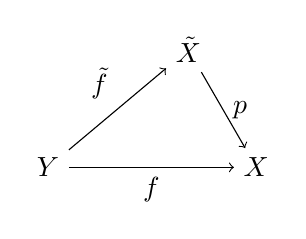
\begin{tikzpicture}[scale=1.15]
  \node (Y)  at (0,0)     {$Y$};
  \node (X)  at (2.3,0)   {$X$};
  \node (Xt) at (1.55,1.3) {$\tilde X$};
  \draw[->] (Y) -- node[below] {$f$} (X);
  \draw[->] (Y) -- node[above left] {$\tilde f$} (Xt);
  \draw[->] (Xt) -- node[right] {$p$} (X);
\end{tikzpicture}
\end{center}
\end{definition}

\Fig[0.62\linewidth]{figures/fig_2_1.png}{2.1}{实直线作为圆周的覆叠空间。}

特别有趣的是道路提升的存在性。这导致 $X$ 与 $\tilde X$ 的基本群之间的联系。

\begin{proposition}[2.4]
设 $f\colon I\to X$ 为端点是 $f(0)=x$ 与 $f(1)=y$ 的道路。对每个 $\tilde x\in p^{-1}(x)$，存在唯一的提升 $\tilde f\colon I\to\tilde X$，满足 $\tilde f(0)=\tilde x$ 且 $p\circ\tilde f=f$。
\end{proposition}

\begin{proof}
取 $X$ 的一个开覆盖 $\{U_a\}$，使得每个开集 $U_a$ 都是覆叠邻域。对每个 $s\in I$ 存在 $s$ 的邻域 $V_s$，使得 $f(V_s)\subset U_a$（对某个 $a$）。于是 $\{V_s\mid s\in I\}$ 是 $I$ 的开覆盖。但 $I$ 紧，由 Lebesgue 引理，存在 $\epsilon>0$，使得当 $|s-t|\le\epsilon$ 时 $f([s,t])\subset U_a$（对某个 $a$）。现在取 $n\in\N$ 使得 $\tfrac{1}{n}<\epsilon$，并令 $s_k=\tfrac{k}{n}$。不妨设 $f(0)\in U_a$。

定义 $\tilde f(0)=\tilde x\in U_a^i\subset p^{-1}(U_a)$，其中 $U_a^i$ 是互不相交的开集，且 $p|_{U_a^i}$ 是同胚。则对每个 $q\in[s_0,s_1]$，有 $f(q)\in U_a$，且 $p\colon U_a^i\to U_a$ 是同胚。我们现在可以定义
\[
\tilde f(q):=p^{-1}\bigl(f(q)\bigr),
\]
对每个 $q\in[s_0,s_1]$。由于 $[s_0,s_1]$ 连通，可知 $\tilde f([s_0,s_1])\subset U_a^i$，因而 $\tilde f|_{[s_0,s_1]}$ 唯一确定。现在通过迭代该过程把 $\tilde f$ 延拓到整个 $I$ 上。
\end{proof}

% [Tutor Note: Lebesgue 引理的正确表述是：紧度量空间 $I$ 的每个开覆盖有 Lebesgue 数 $\epsilon>0$，使直径 $<\epsilon$ 的任意子集都落在某个覆盖元素中。原文用 $|s-t|\le\epsilon$ 并写 $f([s,t])$，隐含 $s<t$。迭代延拓时还须保证每一步的起点落在同一片 $U_a^i$ 内，这由前一步的终点落在该片、且该片经 $p$ 同胚映到 $U_a$ 来保证。]

考虑基点 $x_0\in X$ 与 $\tilde x_0\in p^{-1}(x_0)\subset\tilde X$。

\begin{proposition}[2.5]
基本群上的诱导同态 $p_*\colon\pi_1(\tilde X,\tilde x_0)\to\pi_1(X,x_0)$ 是单射。此外，子群 $p_*\pi_1(\tilde X,\tilde x_0)$ 由以 $x_0$ 为基点且提升为以 $\tilde x_0$ 为基点的环路的那些环路组成。
\end{proposition}

\begin{proof}
对点 $[\tilde f_0]\in\ker(p_*)$，有 $\tilde f_0\colon I\to\tilde X$ 是以 $\tilde x_0$ 为基点的环路，且道路 $f_0=p\circ\tilde f_0$ 同伦于常值道路 $f_1(t)=x_0$（对每个 $t\in I$）。
% [原文 p.15]
对道路 $f_0$ 与 $f_1$ 之间的同伦 $f_t$，可以证明它提升为从 $\tilde f_0$ 到 $\tilde f_1$ 的唯一同伦 $\tilde f_t\colon I\to\tilde X$，满足 $p\circ\tilde f_t=f_t$。于是我们得到 $[\tilde f_0]=1$。
\end{proof}

\begin{proposition}[2.6]
覆叠 $p$ 的叶数等于子群 $p_*\bigl(\pi_1(\tilde X,\tilde x_0)\bigr)$ 在 $\pi_1(X,x_0)$ 中的指数。
\end{proposition}

\begin{proof}
先记 $H:=p_*\bigl(\pi_1(\tilde X,\tilde x_0)\bigr)$。对 $X$ 上以 $x_0$ 为基点的环路 $f$，考虑从右陪集到 $\{p^{-1}(x_0)\}$ 的映射 $\varphi\colon\{H[f]\}\to\{p^{-1}(x_0)\}$，满足 $\varphi(H[f])=\tilde f(1)$，其中 $\tilde f$ 是 $f$ 从点 $\tilde x_0$ 出发的提升。随后可以验证该映射 $\varphi$ 良定义、单射且满射。
\end{proof}

下一个定理对于拓扑空间覆叠空间的分类问题至关重要；我们首先引入如下技术术语：

\begin{definition}[2.7]
若拓扑空间 $X$ 对每个 $x\in X$ 都存在 $x$ 的邻域 $U$，使得同态 $i_*\colon\pi_1(U,x)\to\pi_1(X,x)$ 平凡，则称 $X$ 是\emph{半局部单连通的}。若对每个 $x\in X$ 和 $x$ 的每个邻域 $V$，都存在 $x$ 的邻域 $U\subset V$ 使得 $\pi_1(U,x)=\{e\}$ 平凡，则称 $X$ 是\emph{局部单连通的}。
\end{definition}

\Fig[0.70\linewidth]{figures/fig_2_2.png}{2.2}{夏威夷耳环（左）及其上的锥（右）。}

由
\[
H=\bigcup_{n=1}^{\infty}\Bigl\{(x,y)\in\R^2\ \Big|\ \Bigl(x-\frac{1}{n}\Bigr)^2+y^2=\frac{1}{n^2}\Bigr\}
\]
定义的拓扑空间被称为\emph{夏威夷耳环}；它展示在图 2.2 的左侧。它是非半局部单连通拓扑空间的一个标准例子：$(0,0)$ 的任意邻域都包含无穷多个圆周，从而包含其中的不可缩环路，而这些环路在 $H$ 中仍然不可缩。夏威夷耳环上的锥展示在同一图的右侧；它是一个半局部单连通但非局部单连通的拓扑空间的例子。

% [Tutor Note: “半局部单连通”与“局部单连通”不可混淆。锥 $CH$ 是半局部单连通的：$CH$ 可缩，故 $\pi_1(CH,x)=0$，“同态平凡”自动成立；但它在锥点处不局部单连通（锥点的任意小邻域都含绕锥点的非平凡环路）。核对夏威夷耳环非半局部单连通：任意 $\epsilon$-球内包含无穷多个圆 $(x-\frac1n)^2+y^2=\frac1{n^2}$，且这些小圆在 $H$ 中的同伦类非平凡。]

% [原文 p.16]
\begin{theorem}[2.8]
设 $X$ 是道路连通、局部道路连通且半局部单连通的拓扑空间。则存在 $X$ 的覆叠空间 $\tilde X$，使得 $\pi_1(\tilde X)=1$。空间 $\tilde X$ 称为 $X$ 的\emph{万有覆叠空间}。
\end{theorem}

\begin{remark}[2.9]
在本书后续部分，我们将只关注满足上述定理条件的拓扑流形。因此，读者可以在此背景下理解该定理的陈述与证明。
\end{remark}

\begin{proof}[定理 2.8 的证明]
我们在此只勾勒主要想法；完整证明可参阅例如 [192, Sect. 1.3]。我们可以把 $\tilde X$ 的点视为 $X$ 的点的同伦类，即定义
\[
\tilde X=\bigl\{[\gamma]\ :\ \gamma \text{ 是 } X \text{ 上满足 } \gamma(0)=x_0 \text{ 的道路}\bigr\},
\]
并考虑映射 $p\colon\tilde X\to X$，$p([\gamma])=\gamma(1)$。由于假定 $X$ 道路连通，可推出映射 $p$ 是满射。

对 $x$ 的一个开道路连通邻域 $U$，使得映射 $\pi_1(U,x)\hookrightarrow\pi_1(X,x)$ 平凡，并且对满足 $\gamma(1)\in U$ 的道路 $\gamma$，我们现在可以考察子集族
\[
U_{[\gamma]}:=\bigl\{[\gamma\cdot\eta]\ :\ \eta \text{ 是 } U \text{ 上满足 } \eta(0)=\gamma(1) \text{ 的道路}\bigr\}.
\]
然后可以证明该集族 $U_{[\gamma]}$ 定义了 $\tilde X$ 上一个拓扑的开集基。关于这个拓扑，覆叠映射 $p\colon\tilde X\to X$ 是覆叠空间投影，最后验证 $\tilde X$ 道路连通且单连通。
\end{proof}

\begin{definition}[2.10]
设 $X$ 为道路连通的拓扑空间，$p_1\colon\tilde X_1\to X$、$p_2\colon\tilde X_2\to X$ 为 $X$ 的覆叠空间。若 $f$ 是同胚且 $p_1=p_2\circ f$，则称映射 $f\colon\tilde X_1\to\tilde X_2$ 为\emph{覆叠空间的同构}；若只有后一条件成立，则称 $f$ 为\emph{覆叠空间的同态}。此外，对 $X$ 的覆叠空间 $p\colon\tilde X\to X$，若 $f\colon\tilde X\to\tilde X$ 是覆叠空间的同构，则称 $f$ 为\emph{自同构}。
\end{definition}

覆叠空间的自同构构成一个群，它对我们在后文将要看到的内容具有核心重要性。

\begin{definition}[2.11]
设 $X$ 为道路连通的拓扑空间，$p\colon\tilde X\to X$ 为覆叠空间。自同构 $f\colon\tilde X\to\tilde X$ 称为\emph{覆叠变换}。在环路的拼接运算下，它们构成一个群，记作 $G(\tilde X)$。
\end{definition}

\begin{example}[2.12]
\begin{enumerate}
\item 令 $p\colon\R\to S^1$ 为如例 2.2 中 $p(x)=(\cos(2\pi x),\sin(2\pi x))$ 的单位圆周的覆叠空间，如图 2.1。该覆叠的覆叠变换是由 $x\mapsto x+n$（$n\in\Z$）给出的映射 $f_n\colon\R\to\R$。因此 $G(\tilde\R)\cong\Z$。
\item 令 $p\colon S^1\to S^1$ 为 $p(z)=z^n$（$n\in\Z$）的单位圆周的另一覆叠空间。此时 $G(\tilde{S^1})\cong\Z_n$。
\end{enumerate}
\end{example}

% [Tutor Note: 例 2.12 第 2 条中，$p(z)=z^n$ 要成为覆叠需 $n\ne0$；而 $G(\tilde{S^1})\cong\Z_n$ 的写法默认 $n>0$（$\Z_n$ 表示 $n$ 阶循环群）。核对：$n=2$ 时 $z\mapsto z^2$ 的覆叠变换是 $z\mapsto-z$，群阶为 $2$。]

% [原文 p.17]
注意作用 $G(\tilde X)\curvearrowright X$ 在连通空间 $\tilde X$ 上是\emph{覆叠空间作用}，即对任意点 $\tilde x\in\tilde X$、非平凡 $g\in G(\tilde X)$ 以及覆叠邻域 $\tilde U\ni\tilde x$，有 $g(\tilde U)\cap\tilde U=\varnothing$。特别地，若 $\tilde X$ 是万有覆叠空间，则由于 $G(\tilde X)=\pi_1(X,x_0)$，我们有 $\pi_1(X,x_0)\curvearrowright\tilde X$ 是覆叠空间作用。

% [Tutor Note: 原文此句写作 $G(\tilde X)\curvearrowright X$，目标空间漏了波浪号，应为 $G(\tilde X)\curvearrowright\tilde X$。依据是同句“on the connected space $\tilde X$”，以及紧接着的 $\pi_1(X,x_0)\curvearrowright\tilde X$ 也以 $\tilde X$ 为目标。]

\section{分歧覆叠}

我们在定义 2.1 中已经看到，两个拓扑空间之间的满射 $p\colon\tilde X\to X$ 若通过 $p$ 局部同胚，则为覆叠。这类覆叠实际上称为\emph{非分歧覆叠}。它对 $\tilde X$ 施加许多限制。分歧覆叠的概念灵活得多，它起源于复分析中多值函数的研究。在这些情形中，在底空间的孤立点上方，覆叠的叶可以合并，因此覆叠映射群可以有不动点。

\begin{example}[2.13]
考虑由 $f(z)=z^2$ 给出的映射 $f\colon\C\to\C$。限制到 $\C^*$ 上，它定义了 $2$ 叶覆叠。在原点处，两个叶合并。用下文定义的术语，我们将说原点是\emph{分支点}。
\end{example}

反函数 $z\mapsto\sqrt{z}$ 并非在整个 $\C$ 上良定义。有几种方式理解这个函数。若去掉从原点出发的一条射线（例如负实轴），则平方根是良定义的函数。也可以把 $\sqrt{z}$ 视为多值函数，对每个非零复数有两个值。还有一种方式是：$\sqrt{z}$ 不是 $\C$ 上的良定义函数，而是在由 $f$ 定义的分歧二重覆叠上的良定义函数。平方根的两个可能值分配给两个叶，而当你沿绕原点的环路行进时，就置换了两个叶。

现在我们把分歧覆叠的概念精确化：

\begin{definition}[2.14]
设 $X,\tilde X$ 为两个拓扑曲面。若存在非空离散集 $Y\subset X$，使得 $p|_{p^{-1}(X\setminus Y)}\colon p^{-1}(X\setminus Y)\to X\setminus Y$ 是定义 2.1 意义下的覆叠，则称连续满射 $p\colon\tilde X\to X$ 为（拓扑）\emph{分歧覆叠}。上述子集 $Y$ 称为 $p$ 的\emph{分支轨迹}，我们将把它记作 $B(p)$。点 $b\in Y$ 称为\emph{分支点}。
\end{definition}

我们进一步引入如下术语：

\begin{definition}[2.15]
设 $X,\tilde X$ 与 $p\colon\tilde X\to X$ 如上。考虑点 $\tilde x\in\tilde X$ 及其在 $p$ 下的像 $x:=p(\tilde x)$。映射 $p$ 在点 $\tilde x$ 处的\emph{分歧指数}定义为正整数 $m_{\tilde x}(p)$，使得存在 $\tilde x$ 的开邻域 $U$，点 $x\in X$ 在 $U$ 中只有一个原像，即 $p^{-1}(x)\cap U=\tilde x$，且对其余所有点 $z\in p(U)$ 都有 $|p^{-1}(z)\cap U|=m_{\tilde x}(p)$。若 $m_{\tilde x}(p)>1$，则称点 $\tilde x\in\tilde X$ 为 $\tilde X$ 的\emph{分歧点}。此时 $p(\tilde x)$ 是分支点。此外，映射 $p$ 的\emph{分歧轨迹} $R(p)$ 是 $\tilde X$ 中由所有分歧点构成的子集；另见图 2.3 的例子。
\end{definition}

% [Tutor Note: 定义 2.15 中 $p^{-1}(x)\cap U=\tilde x$ 严格应写作 $p^{-1}(x)\cap U=\{\tilde x\}$：原文把单点集与其元素等同，属记号滥用，引述时勿照抄成集合恒等式。]

% [原文 p.18]
\Fig[0.72\linewidth]{figures/fig_2_3.png}{2.3}{映射 $p\colon\tilde X\to X$ 有两个分支点 $x_1,x_2\in X$ 与两个分歧点 $\tilde x_1,\tilde x_2\in\tilde X$。注意这里 $m_{\tilde x_1}(p)=3$，$m_{\tilde x_2}(p)=2$。}

鉴于上述定义，总有 $R(p)\subseteq p^{-1}(B(p))$。此外，只要 $R(p)=\varnothing$，映射 $p$ 就是非分歧覆叠。当所有分支点的指数为 $2$ 时，我们称之为\emph{简单分歧覆叠}。对每个点 $x\in X$，我们现在考虑映射 $p$ 在各原像处的分歧指数之和：
\[
d_x(p):=\sum_{\tilde x\in p^{-1}(x)}m_{\tilde x}(p).
\]
数 $d_x(p)$ 实际上对一切 $x\in X$ 的点都是常数（证明见 [269, Chap. II, Prop. 4.8]）。于是引出如下定义：

\begin{definition}[2.16]
设 $X,\tilde X$ 与 $p\colon\tilde X\to X$ 如上。映射 $p$ 的\emph{次数}是对任意点 $x\in X$ 的整数 $d_x(p)$，因此将简记为 $\deg(p)$。
\end{definition}

下面的例子给出黎曼曲面上分歧覆叠的局部模型，特别是我们将在 §8.4 进一步讨论的谱曲线。

\begin{example}[2.17]
考虑开集 $U\subset\C$ 与平凡丛 $E=U\times\C$。用 $z$ 表示 $U$ 上的坐标，$p$ 表示纤维上的坐标。对全纯函数 $a_2(z),a_3(z),\dots,a_n(z)$，定义函数
\[
P(p,z)=p^n+a_2(z)p^{n-2}+a_3(z)p^{n-3}+\cdots+a_n(z),
\]
它是 $p$ 的多项式。最后考虑
\[
\tilde U=\{(z,p)\in E\mid P(p,z)=0\}.
\]
把典范投影 $E\to U$ 限制到 $\tilde U$，我们得到覆叠 $\pi\colon\tilde U\to U$，它在多项式 $P$ 的重零点处分歧。$\pi$ 的次数为 $n$，即 $P$ 作为 $p$ 的多项式的次数。若 $P$ 至多有二重零点，则该覆叠是简单分歧的。
\end{example}

% [Tutor Note: 例 2.17 的多项式 $P$ 缺 $p^{n-1}$ 项（其系数取 $0$），这不是笔误：这正是 $\SL_n$ 谱曲线（迹零）的标准形式，与 §8.4 及后文 Hitchin 系统的约定一致；若按一般 $n$ 次多项式补上 $a_1(z)p^{n-1}$，得到的将是 $\GL_n$ 型的谱覆盖。核对方式：$n=2$ 时 $P=p^2+a_2(z)$，对应迹为零的二阶谱曲线。]

现在我们准备陈述拓扑曲面情形下的基本 \emph{Riemann--Hurwitz 公式}：

% [原文 p.19]
\begin{theorem}[2.18]
（Riemann--Hurwitz 公式）设 $S_{g_1,h_1},S_{g_2,h_2}$ 是一对紧连通可定向拓扑曲面，亏格分别为 $g_1$ 与 $g_2$，边界分支数分别为 $h_1$ 与 $h_2$。设 $p\colon S_{g_1,h_1}\to S_{g_2,h_2}$ 为（可能分歧的）拓扑曲面覆叠。则
\[
2g_1+h_1-2=\deg(p)\bigl(2g_2+h_2-2\bigr)+\sum_{x\in S_{g_1,h_1}}\bigl(m_x(p)-1\bigr).
\]
\end{theorem}

证明的想法是：考虑 $S_{g_2,h_2}$ 的一个与分支点相适应的三角剖分（即所有分支点都作为三角剖分的顶点出现），并取它在 $p$ 下的原像，得到 $S_{g_1,h_1}$ 上的一个三角剖分。然后用 Euler 公式 $\chi(S_{g_1,h_1})=V-E+F$ 计算 $S_{g_1,h_1}$ 的 Euler 示性数，其中 $V,E,F$ 分别是 $S_{g_1,h_1}$ 上三角剖分的顶点数、边数与面数。完整证明参见 [269, Chap. II, Prop. 4.16]。

Riemann--Hurwitz 公式是一个强大的工具，应用极多。它的起源可追溯到黎曼曲面的研究，我们将在 §3.1 更仔细地介绍黎曼曲面。黎曼曲面是连通的 $1$ 维复流形；假设黎曼曲面之间的覆叠映射 $p\colon S_{g_1,h_1}\to S_{g_2,h_2}$ 是复解析的，则 $p$ 在点 $x\in S_{g_1,h_1}$ 处分歧，当且仅当 $p$ 在 $x$ 附近的局部坐标 $z$ 下局部表示为 $p(z)=z^n$（对某个整数 $n>1$）。这个数 $n$ 就是点 $x\in S_{g_1,h_1}$ 处的分歧指数。

% [Tutor Note: 可用 $p(z)=z^n\colon\PP^1\to\PP^1$ 核对公式：$g_1=g_2=0$、$h_1=h_2=0$，分支点为 $0$ 与 $\infty$，两处 $m=n$，右端 $=n(-2)+2(n-1)=-2=$ 左端。还须注意求和指标写在上曲面 $S_{g_1,h_1}$ 上（与定义 2.15 的 $m_{\tilde x}$ 一致）；若误改成对底曲面求和，会漏掉分歧贡献。]

除了在本专著的第 II 部分与第 III 部分中的作用之外，分歧覆叠与黎曼曲面还将在第 21、22 章中显著出现，那里将讨论 S 类理论及其 BPS 态。

% [原文 p.20]
% 原文此页为空白页（第 2 章结束后的空白页），无正文。
}{}
\IfFileExists{part/ch03.tex}{% ============================================================
% 第 3 章  丛与联络（Bundles and connections）
% 底本：Springer LNM 2386，Chapter 3，印刷 pp.21–36 / PDF p61–p76
% 交付：work/src/part/ch03.tex（片段，不含导言区）
% ============================================================

\chapter{丛与联络}

% [原文 p.21]
\ChapterAbstract{向量丛上联络的概念，在微分几何与数学物理中都极为重要。借助联络，人们可以理解向量丛在各点处的局部几何，并沿向量场对截面求导。此外，联络还给出曲率这类基本的几何不变量。在物理上，联络被称为规范场或矢量场，其曲率即相应的场强。规范理论为描述物理学中的各种力提供了恰当的数学框架。例如，Maxwell 理论中的相对论性矢量势就是一个联络，而描述电场与磁场的电磁张量正是它的曲率。Riemann–Hilbert 对应把平坦向量丛的几何与底流形的拓扑结构联系起来。本章简要回顾黎曼曲面上带联络的向量丛的理论；若要获得复向量丛微分几何的恰当入门，文献中有大量教材可供查阅，例如 [235] 或 [356]。对物理背景更强的读者，我们热忱推荐 [37]。}

\section{光滑向量丛与全纯向量丛}

% [原文 p.21]
流形理论源于对欧氏空间 $\R^n$ 这一概念的推广，而欧氏空间是这样一个概念：它局部看来就像 $\R^n$。十分类似地，纤维丛理论起源于寻求对流形 $M$ 上取值于某空间 $F$ 的函数 $f\colon M\to F$ 的推广。事实证明，恰当的整体对象是纤维为 $F$ 的丛的截面。这里我们把注意力限制在 $F$ 为向量空间的情形。光滑复向量丛的精确定义在技术上要更繁琐一些。

\begin{definition}[3.1]
设 $E$、$M$ 是两个微分流形，$p\colon E\to M$ 是光滑满射。所谓三元组 $(E,p,M)$ 上的一个\textbf{向量丛图卡}（vector bundle chart），是指一对 $(U,\varphi)$，其中 $U$ 是 $M$ 中的开子集，$\varphi$ 是一个微分同胚，使得下图交换
\[
\begin{array}{ccc}
p^{-1}(U) & \xrightarrow{\ \varphi\ } & U\times\C^{k}\\[4pt]
{\scriptstyle p}\searrow & & \swarrow{\scriptstyle \mathrm{pr}_1}\\[2pt]
& U &
\end{array}
\]
\end{definition}

% [原文 p.22]
\begin{definition}[3.2]
两个向量丛图卡 $(U,\varphi)$ 与 $(V,\psi)$ 称为\textbf{相容的}（compatible），如果映射 $\varphi\circ\psi^{-1}$ 是线性同构，即
\[
\varphi\circ\psi^{-1}(x,\lambda)=(x,\,g_{UV}(x)\cdot\lambda),
\]
其中 $g_{UV}\colon U\cap V\to\GL(\C^k)$ 为某个映射，而 $(x,\lambda)\in V\times\C^k$。此时 $g_{UV}$ 是唯一且光滑的，它称为这两个向量丛图卡之间的\textbf{转移函数}（transition function）。
\end{definition}
% [Tutor Note: 原文 Definition 3.2 的条件写作 “(x,λ) ∈ V × C^k”，应为 $(x,\lambda)\in(U\cap V)\times\C^k$。理由：$\varphi\circ\psi^{-1}$ 只在 $\psi(U\cap V)$ 上有定义（$\psi$ 需 $x\in V$、$\varphi$ 需 $x\in U$），而 $g_{UV}$ 本身是定义在 $U\cap V$ 上的映射，右端 $g_{UV}(x)$ 对 $x\in V\setminus U$ 无意义。核对方法：取 $x\in V\setminus U$，此时 $\varphi(x)$ 不存在，等式两边无法比较。]

\begin{definition}[3.3]
三元组 $(E,p,M)$ 的一个\textbf{向量丛图册}（vector bundle atlas）$(U_\alpha,\varphi_\alpha)_{\alpha\in A}$ 定义为这样一族两两相容的向量丛图卡 $(U_\alpha,\varphi_\alpha)$，使得 $\{U_\alpha\}_{\alpha\in A}$ 是 $M$ 的开覆盖。此外，两个向量丛图册称为\textbf{等价的}（equivalent），如果它们的并仍是向量丛图册。
\end{definition}

\begin{definition}[3.4]
秩为 $k$ 的\textbf{光滑向量丛}是一个三元组 $(E,p,M)$，它由两个光滑流形 $E$、$M$，一个光滑映射 $p\colon E\to M$，以及向量丛图册的一个等价类组成。流形 $E$ 称为\textbf{全空间}（total space），$M$ 称为\textbf{底空间}（base space），$p$ 称为\textbf{投影映射}（projection mapping）。
\end{definition}

复向量空间族 $\{E_x\}_{x\in M}$（其中 $E=\bigcup_{x\in M}E_x$）称为该丛的\textbf{纤维}（fibers）。微分同胚 $\varphi_U\colon p^{-1}(U)\to U\times\C^k$ 把每个向量空间 $E_x$（$x\in U$）同构地映入 $\{x\}\times\C^k$，它称为丛 $E$ 在 $U$ 上的\textbf{局部平凡化}（local trivialization）。向量丛的转移函数所取值的群 $G$ 称为该丛的\textbf{结构群}（structure group）。秩为 $1$ 的向量丛特别地称为\textbf{线丛}（line bundle）。

若 $(U,\varphi)$ 与 $(V,\psi)$ 是向量丛图卡，则对转移函数 $g_{UV}\colon U\cap V\to\GL(\C^k)$，$g_{UV}(x)=(\varphi\circ\psi^{-1})|_{\{x\}\times\C^k}$，下列恒等式成立
\begin{equation}
g_{UV}(x)\cdot g_{VU}(x)=I,\qquad \text{对一切 } x\in U\cap V \tag{3.1}
\end{equation}
\begin{equation}
g_{UV}(x)\cdot g_{VW}(x)\cdot g_{WU}(x)=I,\qquad \text{对一切 } x\in U\cap V\cap W \tag{3.2}
\end{equation}
上述两个恒等式称为\textbf{上循环条件}（cocycle condition），而我们把族 $\{g_{UV}\}$ 称为向量丛图册 $(U_\alpha,\varphi_\alpha)_{\alpha\in A}$ 的\textbf{转移函数上循环}（cocycle of transition functions）。反过来，给定 $M$ 的一个开覆盖 $\{U_\alpha\}_{\alpha\in A}$ 以及光滑映射 $g_{\alpha\beta}\colon U_\alpha\cap U_\beta\to\GL(\C^k)$，只要它们满足上述恒等式，就存在唯一的光滑复向量丛 $(E,p,M)$，其转移函数为 $\{g_{\alpha\beta}\}$。

\begin{definition}[3.5]
向量丛 $E$ 的\textbf{子丛}（subbundle）$F\subset E$ 是纤维 $E_x$ 的一族子空间 $\{F_x\subset E_x\}_{x\in M}$，使得 $F=\bigcup F_x$ 是 $E$ 的子流形。
\end{definition}

\begin{definition}[3.6]
两个光滑向量丛 $E$ 与 $F$ 之间的\textbf{向量丛同态}（vector bundle homomorphism）是一个光滑映射 $f\colon E\to F$，使得 $f(E_x)\subset F_x$，且
\end{definition}

% [原文 p.23]
$f_x=f|_{E_x}\colon E_x\to F_x$ 是复向量空间的线性映射。此外，两个光滑向量丛 $E$、$F$ 称为\textbf{同构的}（isomorphic），如果存在向量丛同态 $f\colon E\to F$，使得对一切 $x\in M$，$f_x\colon E_x\to F_x$ 都是复向量空间的同构。

秩为 $k$ 的光滑向量丛称为\textbf{平凡的}（trivial），如果它同构于 $M\times\C^k$。

上述定义中一个重要的特殊情形是 $E=F$，此时我们得到\textbf{丛自同构}（bundle automorphism）的概念，它也称为\textbf{规范变换}（gauge transformation）。

\begin{definition}[3.7]
对光滑复向量丛 $V$，\textbf{规范变换}（gauge transformation）定义为丛 $V$ 的光滑自同构。$V$ 的全体规范变换所成的集合称为 $V$ 的\textbf{规范群}（gauge group）。
\end{definition}

既然已经引入了向量丛，那么推广了向量值函数概念的\textbf{截面}（section）概念便自然而然地接踵而至：

\begin{definition}[3.8]
光滑向量丛 $(E,p,M)$ 的一个\textbf{截面}是一个光滑映射 $\sigma\colon M\to E$，使得对每个 $x\in M$ 都有 $\sigma(x)\in E_x$。截面空间记作 $\mathcal{A}^0(M;E)$。类似地，我们用 $\mathcal{A}^k(M;E)$ 记 $M$ 上取值于 $E$ 的光滑微分 $k$-形式所成的空间。
\end{definition}

\begin{definition}[3.9]
丛 $E$ 在 $U\subset M$ 上的一个\textbf{光滑局部标架}（local frame）是一族光滑截面 $\sigma_1,\dots,\sigma_k$，使得对每个 $x\in U$，$\{\sigma_1(x),\dots,\sigma_k(x)\}$ 都是复向量空间 $E_x$ 的一组基。
\end{definition}

秩为 $k$ 的光滑向量丛 $E$ 在 $U$ 上的光滑局部标架，实际上就是 $E$ 在 $U$ 上的一个平凡化。事实上，给定平凡化 $\varphi_U\colon E_U=p^{-1}(U)\to U\times\C^k$，则截面
\[
\sigma_i(x)=\varphi_U^{-1}(x,e_i)
\]
构成一个光滑标架。反之，若 $\sigma_1,\dots,\sigma_k$ 是光滑标架，则可定义平凡化 $\varphi_U$ 为
\[
\varphi_U(\lambda)=(x,(\lambda_1,\dots,\lambda_k)) ,
\]
其中 $\lambda=\sum\lambda_i\sigma_i(x)\in E_x$。

\begin{remark}[3.10]
局部地，在丛 $V$ 上选定一个标架之后，规范变换就是一个取值于 $\GL_n(\C)$ 的 $C^\infty$-映射。
\end{remark}

下面我们以与光滑向量丛类似的方式定义全纯向量丛。为此，需要一个复的底流形。

\begin{definition}[3.11]
（复）维数为 $n$ 的\textbf{复流形}（complex manifold）$M$ 是一个微分流形，它容许一个开覆盖 $\{U_\alpha\}_{\alpha\in A}$ 以及转移函数 $\varphi_\alpha\colon U_\alpha\to\C^n$，使得对一切 $\alpha$ 与 $\beta$，$\varphi_\alpha\circ\varphi_\beta^{-1}$ 在 $\varphi_\beta(U_\alpha\cap U_\beta)\subset\C^n$ 上全纯。维数为 $1$ 的复流形称为\textbf{黎曼曲面}（Riemann surface）。
\end{definition}

% [原文 p.24]
\begin{definition}[3.12]
设 $M$ 是复流形。秩为 $k$ 的\textbf{全纯向量丛}（holomorphic vector bundle）$(E,p,M)$ 是一个光滑复向量丛，并具有如下附加性质：$E$ 上赋予了一个复流形结构，使得对每个 $x\in M$ 都存在包含 $x$ 的开集 $U\subset M$ 以及平凡化 $\varphi_U\colon E_U\to U\times\C^k$，它是复流形之间的双全纯映射。
\end{definition}

这样的平凡化称为\textbf{全纯平凡化}（holomorphic trivialization）。此外，与光滑复向量丛的情形类似，给定全纯向量丛的一族平凡化 $\{\varphi_\alpha\colon E_{U_\alpha}\to U_\alpha\times\C^k\}$，关于这族平凡化的转移函数便是全纯的。反过来，给定满足恒等式 (3.1)、(3.2) 的全纯映射 $g_{\alpha\beta}\colon U_\alpha\cap U_\beta\to\GL\big(\C^k\big)$，我们可以构造一个以 $g_{\alpha\beta}$ 为转移函数的全纯向量丛。

我们关于光滑复向量丛所讨论的一切方面，都可类似地适用于全纯向量丛这一范畴，区别只在于此处的定义中诸映射都要求是全纯的。

作为例子，我们来分析黎曼球面上的全纯线丛。

\begin{example}[3.13]
\textbf{黎曼球面}（Riemann sphere）$\C\PP^1$ 由两个图卡 $U_0=\C$ 与 $U_1=\C$ 给出，转移映射 $U_0\cap U_1=\C^\ast\to\C^\ast$ 为 $z\mapsto 1/z$。如下定义线丛 $\OO(k)$：它由两块 $U_0\times\C$ 与 $U_1\times\C$ 组成，二者通过映射
\[
\begin{array}{rcl}
(U_0\cap U_1)\times\C & \to & (U_0\cap U_1)\times\C\\[2pt]
(z,v) & \mapsto & (1/z,\,z^{k}v)
\end{array}
\]
粘合起来。可以证明，同构意义下，线丛 $\OO(k)$ 描述了 $\C\PP^1$ 上所有的全纯线丛。
\end{example}

对任意向量丛 $E\to M$，我们可以如下方式联系一个线丛。取 $M$ 的一个开覆盖，由 $E$ 在其上平凡的开集 $U_\alpha$ 组成，其转移映射为 $f_{\alpha\beta}$。定义\textbf{行列式线丛}（determinant line bundle）$\det(E)$ 为在 $U_\alpha$ 上平凡、转移函数为 $\det\big(f_{\alpha\beta}\big)$ 的线丛。

对一般的复流形，一个重要全纯丛是典范丛：

\begin{definition}[3.14]
复流形 $X$ 的\textbf{典范丛}（canonical bundle）$K_X$ 是联系于全纯余切丛 $T^\ast X$ 的行列式线丛。等价地，它是全纯 $n$-形式所成的线丛，其中 $n$ 是 $X$ 的维数。
\end{definition}

在紧拓扑曲面 $S$ 上，复向量丛很容易分类。线丛的同构类由其\textbf{次数}（degree）或\textbf{第一陈类}（first Chern class）唯一确定，后者是 $H^2(S,\Z)\cong\Z$ 中的一个元素。高阶的复向量丛则由其行列式线丛分类：

\begin{proposition}[3.15]
曲面 $S$ 上秩为 $k$ 的复丛 $E\to S$ 同构于 $\det(E)\oplus\C^{k-1}$（作为复丛）。
\end{proposition}
% [Tutor Note: 命题 3.15 的“证明”原文省略，依据可用障碍论补出：曲面 $S$ 是二维 CW 复形，而 $\mathrm{BU}(k)$ 单连通且 $\pi_2(\mathrm{BU}(k))\cong\Z$、更高同伦群在维数 $\le 2$ 的障碍中不出现，故 $[S,\mathrm{BU}(k)]\cong H^2(S;\Z)$，即秩为 $k$ 的复丛在同构意义下只由第一陈类 $c_1$ 决定。而 $\det(E)\oplus\C^{k-1}$ 与 $E$ 同秩且同 $c_1$（因为 $c_1(\det E\oplus\C^{k-1})=c_1(\det E)=c_1(E)$），故二者同构。核对方法：$k=1$ 时命题退化为 $\det(E)=E$，自洽。]

% [原文 p.25]
全纯丛要丰富得多。在亏格至少为 $2$ 的紧黎曼曲面 $X$ 上，存在全纯线丛的光滑族，由\textbf{皮卡簇}（Picard variety）所描述。次数为零的线丛由\textbf{雅可比簇}（Jacobian variety）参数化。$X$ 上高阶全纯丛的模空间可以借助 Mumford [276] 的\textbf{斜率稳定性}（slope stability）概念来构造。

为结束本节，我们给出一个说明复丛与全纯丛之区别的例子：

\begin{example}[3.16]
在 $\C\PP^1$ 上考虑全纯秩二丛 $\OO(1)\oplus\OO(1)$。其底层的复向量丛是 $\C\oplus T\C\PP^1$，因为容易验证 $\det(\OO(1)\oplus\OO(1))=\OO(2)$，而后者正是 $\C\PP^1$ 的切丛。注意 $\C\oplus T\C\PP^1$ 不是平凡的，因为 $T\C\PP^1$ 没有处处非零的截面（即“毛球定理”）。
\end{example}

注意其底层的实丛是平凡的。可以验证 $T(\mathbb{S}^2)\oplus\R$ 是平凡丛。事实上，只需取单位球面 $\mathbb{S}^2\subset\R^3$ 并考虑其法丛，后者是平凡的（存在常值截面）。于是它与切丛的直和给出 $\R^3$ 的切丛，而后者限制在球面上是平凡的。因此 $T(\mathbb{S}^2)\oplus\R^2\cong\R^4$。

\section{联络}

% [原文 p.25]
联络使人们能够定义截面的方向导数。它们借助平行移动的概念，把同一纤维丛的不同纤维联系起来。

\begin{definition}[3.17]
设 $V$ 是复流形 $M$ 上秩为 $n$ 的光滑复向量丛。我们定义 $V$ 上的一个\textbf{联络}（connection）为一个光滑线性映射
\[
d_A\colon \mathcal{A}^0(M;V)\to\mathcal{A}^1(M;V)\cong\mathcal{A}^1(M)\otimes\mathcal{A}^0(M,V) ,
\]
它满足莱布尼茨法则
\begin{equation}
d_A(fs)=\de f\otimes s+f\,d_A s , \tag{3.3}
\end{equation}
其中 $f$ 是任意光滑函数，$s\in\mathcal{A}^0(M;V)$ 是任意截面。
\end{definition}

设 $e=(e_1,\dots,e_n)$ 是丛 $V$ 的一个局部标架。于是我们可以把 $d_Ae_i$ 写成该标架各元素的线性组合：
\[
d_Ae_i=\sum A_i^{\,j}e_j .
\]
由 $1$-形式构成的矩阵 $A=(A_{ij})$ 称为 $d_A$ 关于标架 $e$ 的\textbf{联络矩阵}（connection matrix）。\footnote{在规范理论中，联络被视为底流形 $M$（它常被解释为时空流形）上的场。它们被称为规范场，而其量子称为规范玻色子。一个简单的例子是电磁学中的（相对论性）矢量势，它是一个 $1\times 1$ 的 $1$-形式矩阵，局部地表示时空上线丛上的一个联络。}

% [原文 p.26]
由此可见，标架与联络矩阵完全决定了联络；事实上，把任意截面 $s\in\mathcal{A}^0(M;V)$ 写成 $s=\sum s^ie_i$ 的形式，其中 $s^i\in C^\infty(M)$，我们便有
\[
d_As=\sum \de s^i\otimes e_i+\sum s^i\cdot d_Ae_i=\sum_j\Big(\de s^j+\sum_i s^iA_i^{\,j}\Big)e_j .
\]
于是，考虑丛 $V$ 的一个局部标架 $e=(e_1,\dots,e_n)$，联络可以局部地写成
\[
d_A=\de+A=\de+\sum_i A_i\de x_i ,
\]
其中我们在 $M$ 上固定了局部坐标 $(x_1,\dots,x_n)$ 给出 $1$-形式 $\de x^i$，$A$ 是联络矩阵，而 $A_i$ 是元素为 $M$ 上 $C^\infty$-函数的矩阵。
% [Tutor Note: 本页公式 $d_A=\de+A=\de+\sum_i A_i\de x_i$ 与紧接其后的文字 “the 1-forms $\de x^i$” 上下标不一致（求和号下的 $A_i$ 与 $\de x_i$ 都是下标，正文却写 $\de x^i$）；同页上文的矩阵记号 $A=(A_{ij})$ 与前页的 $d_Ae_i=\sum A_i^{\,j}e_j$ 也不一致。统一的约定是：$A_i^{\,j}$ 的第一个下标 $i$ 是“标架指标”（行）、第二个 $j$ 是“分量指标”（列），$A_i$ 是 $\de/\de x^i$ 方向的矩阵值系数，而 $A=\sum_i A_i\de x^i$。核对方法：把 $d_A$ 作用在 $e_i$ 上并令 $f=1$，即得 $d_Ae_i=Ae_i=\sum_j A_i^{\,j}e_j$；再把 $A=\sum_i A_i\de x^i$ 展开即可读出 $\de x^i$ 的系数是 $A_i$。]

然而，对于一点 $z\in M$，联络矩阵 $A$ 依赖于 $z$ 的邻域中标架的选取。事实上，若在 $z$ 的邻域中另取标架 $e'$，则 $d_A$ 关于 $e'$ 的联络矩阵可写成
\begin{equation}
A_{e'}=g^{-1}\cdot(\de g)+g^{-1}\cdot A_e\cdot g ; \tag{3.4}
\end{equation}
上式刻画了规范变换群在联络空间上的作用。

联络的局部表达式使我们认识到：联络提供了一种手段，沿着底流形上的曲线，以平行的方式在向量丛的各纤维之间搬运向量。下面我们来描述这一图景。

\begin{definition}[3.18]
设 $(E,p,M)$ 是带有联络 $d_A$ 的光滑复向量丛。$E$ 的一个局部截面 $s$ 称为关于联络 $d_A$ 的\textbf{平行}（parallel）截面，如果 $d_As=0$。
\end{definition}

考虑流形 $M$ 上的光滑曲线 $c\colon[0,1]\to M$。关于一个局部标架，条件 $\de_{c'(t)}s=0$（对一切 $t\in[0,1]$）可以表示为一阶线性常微分方程组：
\begin{equation}
\frac{\de s^i}{\de t}+\sum_{i,j}A_i^{\,j}(c'(t))s^j=0 , \tag{3.5}
\end{equation}
其中 $(A_i^{\,j})$ 是 $d_A$ 关于所选局部标架的联络矩阵的矩阵元。若初始条件由一点 $v\in E_{c(0)}$ 给出，则方程组 (3.5) 的解是一个依赖于时间的截面 $s$，使得 $s(c(0))=v$ 且 $\de_{c'(t)}s=0$。常微分方程组理论的标准技术给出方程组 (3.5) 解的存在唯一性；此外，这些解对一切 $t\in[0,1]$ 都有定义，因为联络矩阵中出现的 $1$-形式 $A_i^{\,j}$ 是光滑的，而我们的方程组是一阶线性的。因此，这个满足 $s(c(0))=v$ 且 $\de_{c'(t)}s=0$ 的、依赖于时间的唯一平行截面 $s\in\mathcal{A}^0(E)$ 是良定义的，它称为 $v$ 沿曲线 $c$ 的\textbf{平行移动}（parallel transport），或称为沿 $c$ 的平行截面。我们作如下定义：
% [Tutor Note: 式 (3.5) 左端对 $i$ 是自由的（$\de s^i/\de t$ 中 $i$ 不求和），右端求和却写成 $\sum_{i,j}$；按下一行“$(A_i^{\,j})$ 是联络矩阵的矩阵元”的说明，正确的形式是 $\dfrac{\de s^i}{\de t}+\sum_j A_i^{\,j}(c'(t))\,s^j=0$，即求和只对列指标 $j$ 进行。核对方法：$n=1$ 时该式退化为 $\de s/\de t+A(c'(t))s=0$，此时 $\sum_{i,j}$ 与 $\sum_j$ 无差别，须用 $n\ge2$ 且取定 $i$ 来检验。]

% [原文 p.27]
\begin{definition}[3.19]
设 $(E,p,M)$ 是光滑复向量丛，$c\colon[0,1]\to M$ 是底流形 $M$ 上的光滑曲线。对固定的 $t\in[0,1]$，沿曲线 $c$ 从 $c(0)$ 到 $c(t)$ 的\textbf{平行移动}是一个线性映射
\[
P_{c(t)}\colon E_{c(0)}\to E_{c(t)} ,
\]
它把点 $v\in E_{c(0)}$ 映到向量 $P_{c(t)}(v)=s(c(t))\in E_{c(t)}$，其中 $s$ 是沿曲线 $c$ 的唯一平行截面且 $s(c(0))=v$。
\end{definition}

于是，联络给出了一种把曲线从底流形提升到丛中的方式，而平行移动映射是向量丛各纤维之间的线性同构；见图 3.1。

\Fig[0.45\linewidth]{figures/fig_3_1.png}{3.1}{沿 $M$ 上道路 $c$ 的平行移动。}

\section{曲率与平坦性}

% [原文 p.28]
我们在研究联络时描述了两个主要视角：一个是整体的，把联络看作微分算子；另一个则借助标架，考虑联络作为 $1$-形式矩阵的局部表达式，并给出沿底流形上曲线作平行移动的手段。光滑复向量丛上任意给定联络的\textbf{曲率}（curvature）可用类似方式整体地定义，即作为唯一延拓联络所定义的算子而得到的二阶线性微分算子；它也可以局部地用 $2$-形式矩阵来描述。

\begin{definition}[3.20]
设 $(V,p,M)$ 是带有联络 $d_A$ 的光滑复向量丛。我们定义 $d_A$ 在 $V$ 上的\textbf{曲率}为算子
\[
F_A=d_A^2\colon \mathcal{A}^0(M;V)\to\mathcal{A}^2(M;V) ,
\]
它是光滑线性映射，并且可视为
\[
\mathcal{A}^2(M;\End V)=\mathcal{A}^2(\Hom(V,V))
\]
中的一个元素。
\end{definition}

与联络类似，我们可以关于丛的一个标架局部地表示曲率算子。事实上，设 $e=(e_1,\dots,e_n)$ 是丛 $V$ 的局部标架。我们把 $F_Ae_i$ 写成标架各元素的线性组合
\[
F_A(e_i)=\sum\Theta_i^{\,j}e_j .
\]
这个 $2$-形式矩阵 $\Theta_e=(\Theta_i^{\,j})$ 称为该联络的\textbf{曲率矩阵}（curvature matrix）。对局部标架的另一选取 $e'=(e'_1,\dots,e'_n)$，可以验证
\[
\Theta_{e'}=g^{-1}\cdot\Theta_e\cdot g .
\]
我们也可以用联络矩阵来表达曲率矩阵。事实上，下列公式容易建立
\begin{equation}
\Theta_e=\de A_e+A_e\wedge A_e , \tag{3.6}
\end{equation}
它通常称为 \textbf{Cartan 结构方程}（Cartan structure equation）。\footnote{在物理上，曲率算子称为相应规范场的场强。在电磁学中，矢量势的场强就是电磁张量，它描述电场与磁场。}

\begin{definition}[3.21]
若光滑复向量丛上某联络的曲率 $F_A$ 处处为零，则称该联络是\textbf{平坦的}（flat）。
\end{definition}

\begin{proposition}[3.22]
若 $d_A$ 是平坦联络，则方程 $d_As=0$ 存在 $n$ 个线性无关的局部解。
\end{proposition}

\begin{proof}
只需说明存在由平行截面构成的局部标架 $e=(s_1,\dots,s_n)$。$d_A$ 关于这样一个局部标架的矩阵 $A$ 是
% [原文 p.29]
零矩阵。设 $e'=(e'_1,\dots,e'_n)$ 是局部标架，$A'$ 是 $d_A$ 关于 $e'$ 的联络矩阵。正如前面所提到的，从标架 $e$ 到 $e'$ 的过渡由两个标架相应矩阵之间的如下关系决定：$A=g^{-1}(\de g)+g^{-1}A'g$。于是，条件 $A=0$ 等价于线性微分方程组
\begin{equation}
g^{-1}(\de g)+g^{-1}A'g=0 . \tag{3.7}
\end{equation}
因此，为这个线性微分方程组找到一个解 $g$，等价于证明存在由平行截面构成的标架。现在，用 $g$ 取式 (3.7) 的像，我们得到 $A'g+\de g=0$，对其求导便得到积分条件
\[
0=(\de A')g-A'\wedge \de g=(\de A')g+(A'\wedge A')g=\Theta'g ,
\]
其中用到 $\de g=-A'g$ 以及上面的 Cartan 结构方程 (3.6)。

于是我们看到，这个方程组的积分条件恰好是矩阵 $\Theta'$ 的消失，而这一条件与局部标架的选择无关。因此，若联络是平坦的，则显然曲率矩阵是零矩阵；于是，由线性微分方程组解的存在性，我们所求的解 $g$ 存在。
\end{proof}
% [Tutor Note: 证明末句“由线性微分方程组解的存在性”跳过了标准论证：$\Theta'=0$ 时 $A'$ 满足 $\de A'+A'\wedge A'=0$，即该联络的曲率形式为零，这正是方程组 $A'g+\de g=0$（等价于 $g^{-1}\de g=-g^{-1}A'g$）的 Frobenius 可积性条件；在单连通邻域上由 Frobenius 定理（或 Poincaré 引理加逐次积分）即得局部解 $g$，且 $g$ 取值于 $\GL_n(\C)$（因初值 $g(z_0)=I$ 附近 $\det g\neq0$）。核对方法：把 $A'g+\de g=0$ 写成 $\de g=-A'g$，求导得 $0=\de^2g=(\de A')g-A'\wedge\de g$，代入 $\de g=-A'g$ 即得 $(\de A'+A'\wedge A')g=0$，与 (3.6) 一致。]

\begin{remark}[3.23]
若有这样两组解构成的基 $(e_1,\dots,e_n)$ 与 $(\tilde e_1,\dots,\tilde e_n)$，其中 $\tilde e_i=\sum a_i^{\,j}e_j$，则
\[
0=d_A\tilde e_i=d_A\Big(\sum a_i^{\,j}e_j\Big)=\sum \de a_i^{\,j}\otimes e_j ,
\]
于是 $\de a_i^{\,j}=0$，即 $a_i^{\,j}$ 是常值函数。
\end{remark}

我们由此得出结论：平坦联络诱导出丛 $V$ 的一族\textbf{局部常值转移函数}。其逆亦真：若 $V$ 具有局部常值的转移函数，则它容许一个平坦联络。事实上，若 $\{U,e_U\}$ 是丛的一族具有常值转移函数的局部标架，我们定义联络 $d_A$ 为 $d_Ae_U=0$。于是，由于转移函数是常值的，条件 $d_Ae_U=0$ 与 $d_Ae_W=0$ 在 $U\cap W\subset V$ 上相容，故该联络良定义。现在显然这个联络是平坦的。带有平坦联络的丛称为\textbf{局部系统}（local system）。

\section{Riemann–Hilbert 对应}

% [原文 p.29]
下面我们将看到一个深刻的等价性：流形 $M$ 的基本群的表示 $\rho\colon\pi_1(M)\to\GL_n(\C)$，与 $M$ 上秩为 $n$ 的平坦 $C^\infty$-复向量丛 $E$ 之间的等价性。$\rho$ 的像 $H$ 称为\textbf{和乐群}（holonomy group）。我们首先由一个表示构造出平坦丛。

% [原文 p.30]
设 $\rho\colon\pi_1(M)\to\GL_n(\C)$ 是基本群的一个表示。我们把 $\pi_1(M)$ 视为作用在 $M$ 的泛覆叠空间 $\tilde M$ 上的覆叠变换群，并考虑作用
\[
\delta\colon \pi_1(M)\to\Homeo(\tilde M\times\C^n)
\]
它由 $\delta(\gamma)(x,v)=(\gamma(x),\rho(\gamma)^{-1}\cdot v)$ 给出。这个作用诱导出交换图
\[
\begin{array}{ccc}
\tilde M\times\C^n & \xrightarrow{\ \mathrm{pr}\ } & \tilde M\\[6pt]
{\scriptstyle \pi}\downarrow & & {\scriptstyle q}\downarrow\\[6pt]
E=(\tilde M\times\C^n)/\delta & \xrightarrow{\ p\ } & M ,
\end{array}
\]
其中 $\mathrm{pr}$ 是自然投影（它显然是等变的），$\pi$ 是商映射，$q$ 是覆叠映射，而 $p$ 由投影 $\mathrm{pr}$ 唯一诱导。于是我们可以证明：

\begin{proposition}[3.24]
对上述图表，有
\begin{enumerate}[label=\arabic*.]
\item 映射 $\pi\colon\tilde M\times\C^n\to E$ 是覆叠映射。
\item 若和乐群 $H=\op{Im}\rho$ 带有从 $\GL_n(\C)$ 诱导的拓扑，则 $\xi_H=(E,p,M)$ 是一个平坦的 $C^\infty$ 复向量丛，其结构群为离散群 $H$。
\end{enumerate}
\end{proposition}

\begin{proof}
\begin{enumerate}[label=\arabic*.]
\item 由于作用 $\delta$ 是自由且真不连续的，故映射 $\pi$ 是覆叠映射。
\item 我们取 $M$ 的一个由可缩集构成的开覆盖 $\{U_i\}$。此外，对每个 $i$，我们取一点 $b_i\in U_i$ 以及一条从 $b_0$ 到 $b_i$ 的道路 $c_i$，其中 $b_0\in M$ 是基点，换言之 $\pi_1(M)=\pi_1(M,b_0)$。

对每个 $U_i$，我们要求一个平凡化 $\varphi_i\colon p^{-1}(U_i)\to U_i\times\C^n$。设 $\tilde c_i$ 是道路 $c_i$ 从基点 $\tilde b_0\in q^{-1}(b_0)\subset\tilde M$ 出发的提升，而 $\tilde U_i$ 是 $q^{-1}(U_i)$ 中包含道路 $\tilde c_i$ 终点的子集。由于 $\pi_1(M,b_0)$ 的每个非平凡元素都交换 $\mathrm{pr}^{-1}(q^{-1}(U_i))$ 的各个子集，故
\[
\pi_i:=\pi|_{\tilde U_i\times\C^n}\colon \tilde U_i\times\C^n\to p^{-1}(U_i)
\]
是同胚。于是
\[
\varphi_i=q|_{\tilde U_i\times\C^n}\circ\pi_i^{-1}\colon p^{-1}(U_i)\to U_i\times\C^n
\]
是丛 $\xi_H$ 在 $U_i$ 上的局部平凡化，这由交换图的可交换性可得。

现在，设 $U_i$、$U_j$ 是 $M$ 的覆盖中两个满足 $U_i\cap U_j\neq\varnothing$ 的元素。对每个 $b\in U_i\cap U_j$，我们考虑 $U_i$ 上从 $b_i$ 到 $b$ 的道路 $w_{ib}$，以及从 $b_j$ 到 $b$ 的道路 $w_{jb}$。则回路 $\gamma_{ij}=\big[c_i\circ w_{ib}\circ w_{jb}^{-1}\circ c_j^{-1}\big]\in\pi_1(M,b_0)$（这里 $\circ$ 表示道路的衔接）不依赖于 $w_{ib}$ 与 $w_{jb}$ 的选取（图 3.2）。于是可知，映射
% [原文 p.31]
\Fig[0.75\linewidth]{figures/fig_3_2.png}{3.2}{以 $b_0$ 为基点的回路的构造。}
\[
g_{ij}\colon U_i\cap U_j\to\op{Im}\rho
\]
把 $b$ 映到 $\rho(\gamma_{ij})$，故它是局部常值的。因此，我们构造出了一个具有局部常值转移函数的向量丛，于是由注 3.23，该丛是平坦的。
\end{enumerate}
\end{proof}
% [Tutor Note: 原文 “Since every non trivial element of π₁(M,b₀) commutes the subsets of pr⁻¹(q⁻¹(U_i))” 中的 “commutes” 应是 “permutes”（置换）：$\pi_1(M,b_0)$ 通过覆叠变换作用在 $\tilde M\times\C^n$ 上，从而置换 $\mathrm{pr}^{-1}(q^{-1}(U_i))$ 的各连通分支（即各“叶”）；正因如此，$\tilde U_i$ 所代表的这一叶在商掉 $\delta$ 后与 $p^{-1}(U_i)$ 一一对应，$\pi_i$ 才是同胚。照原文直译作“交换”，但数学含义是“置换”。核对方法：$U_i$ 可缩时 $q^{-1}(U_i)$ 是 $|H|$ 个不交叶的并，$\delta$ 置换这些叶而不固定任何一片（自由性），故限制在单片 $\tilde U_i$ 上即为单射且满。]

我们已经看到，表示 $\rho\colon\pi_1(M)\to\GL_n(\C)$ 决定了 $M$ 上一个秩为 $n$、具有局部常值转移函数的光滑复向量丛 $E$。接下来我们将看到，所有具有局部常值转移函数的光滑复向量丛实际上都是这样构造出来的。

\begin{definition}[3.25]
设 $(E,p,M)$ 是 $C^\infty$-复向量丛，其转移函数局部常值、取值于结构群 $G\subseteq\GL_n(\C)$，并设 $F_0$、$F_1$ 分别是 $b_0,b_1\in M$ 上的纤维。若 $c\colon[0,1]\to M$ 是从 $b_0$ 到 $b_1$ 的道路，则对每个 $y\in F_0$，道路 $c$ 从 $y$ 出发的提升 $\tilde c_y$ 存在且唯一。于是我们可以定义一个同胚
\[
T_c\colon F_0\to F_1 ,
\]
它称为沿 $c$ 把 $F_0$ \textbf{平移}（translation）到 $F_1$，并且它只依赖于 $c$ 的同伦类（端点固定）。
\end{definition}

若现在取 $b_0=b_1$，并固定一个满足 $b_0\in U_0$ 的平凡化 $(U_0,\varphi_0)$，则对每个 $\gamma\in\pi_1(M)$ 都构造出一个同胚 $T_\gamma\in G$。容易看出 $T_{\gamma\gamma'}=T_{\gamma'}\circ T_\gamma$。于是，若对丛 $\xi$ 定义 $H_\xi(\gamma)=T_\gamma^{-1}$，则映射
\[
H_\xi\colon \pi_1(M)\to G
\]
是一个同态，它称为丛 $\xi$ 的\textbf{和乐表示}（holonomy representation，或\textbf{单值表示} monodromy representation）。
% [Tutor Note: 这里 $T_{\gamma\gamma'}=T_{\gamma'}\circ T_\gamma$ 的“反序”与 $H_\xi(\gamma)=T_\gamma^{-1}$ 的“取逆”必须配套，否则 $H_\xi$ 不是同态：$H_\xi(\gamma\gamma')=T_{\gamma\gamma'}^{-1}=(T_{\gamma'}\circ T_\gamma)^{-1}=T_\gamma^{-1}\circ T_{\gamma'}^{-1}=H_\xi(\gamma)\circ H_\xi(\gamma')$。原因是对道路拼接按“先走 $\gamma$、再走 $\gamma'$”定义，而平移 $T_\gamma$ 是把起点纤维搬到终点纤维，故复合次序相反；取逆恰好把它翻转为左作用下的同态。核对方法：取 $n=1$、$\gamma'=\gamma^{-1}$，则 $H_\xi(\gamma)H_\xi(\gamma^{-1})=T_\gamma^{-1}T_{\gamma^{-1}}^{-1}=T_\gamma^{-1}T_\gamma=\mathrm{id}$。]

\begin{definition}[3.26]
设 $p\colon\tilde M\to M$ 是覆叠空间投影，$\gamma$ 是 $M$ 上以 $x_0\in M$ 为基点的回路，它唯一地提升为 $\tilde M$ 中以一点
% [原文 p.32]
$y_0\in p^{-1}(x_0)$ 为基点的道路 $\tilde\gamma$。对点 $x_0$，定义\textbf{单值作用}（monodromy action）为群 $\pi_1(M,x_0)$ 在 $p^{-1}(x_0)$ 上的右群作用
\[
\begin{array}{rcl}
p^{-1}(x_0)\times\pi_1(M,x_0) & \to & p^{-1}(x_0)\\[2pt]
(y_0,[\gamma]) & \mapsto & \tilde\gamma(1) .
\end{array}
\]
\end{definition}

联系于单值作用的表示 $\rho\colon\pi_1(M,x_0)\to\GL(p^{-1}(x_0))$ 称为\textbf{单值表示}（monodromy representation）。两个单值表示 $\rho$ 与 $\rho'$ 称为\textbf{等价的}，如果对每个同伦类 $[\gamma]\in\pi_1(M,x_0)$，都存在纤维 $p^{-1}(x_0)$ 的一个线性自同构 $A\in\GL(p^{-1}(x_0))$，使得 $\rho'([\gamma])=A\rho([\gamma])A^{-1}$。

\begin{proposition}[3.27]
纤维为 $\C^n$、转移函数局部常值且取值于结构群 $G\le\GL_n(\C)$ 的 $C^\infty$-向量丛 $\xi=(E,p,M)$ 是平凡的，当且仅当其和乐表示是平凡的。
\end{proposition}

\begin{proof}
正向显然。为证反向，设
\[
H_\xi\colon \pi_1(M)\to G
\]
是平凡的。则对 $M$ 中任意以 $b$ 为起点、以 $b_0$ 为终点的道路 $c$，平移 $T_c\colon F_b\to F_{b_0}$ 不依赖于道路 $c$，以下记作 $T_b$。我们可以通过相应的图卡把纤维 $F_{b_0}$ 与 $\C^n$ 等同，于是映射 $h\colon E\to M\times\C^n$，$x\mapsto(p(x),T_{p(x)}(x))$ 是一个同构。
\end{proof}

\begin{theorem}[3.28]
每个转移函数局部常值、取值于群 $G\le\GL_n(\C)$ 的向量丛 $\xi=(E,p,M)$，都同构于由某个表示 $H_\xi\colon\pi_1(M)\to G$ 所诱导的向量丛。
\end{theorem}

\begin{proof}
设 $\tilde\xi=(\tilde E,\tilde p,\tilde M)$ 是由泛覆叠 $q\colon\tilde M\to M$ 所诱导的向量丛。于是我们有交换图
\[
\begin{array}{ccc}
\tilde E & \xrightarrow{\ \tilde p\ } & \tilde M\\[6pt]
{\scriptstyle \pi}\downarrow & & {\scriptstyle q}\downarrow\\[6pt]
E & \xrightarrow{\ p\ } & M .
\end{array}
\]
由于泛覆叠空间 $\tilde M$ 单连通，我们有 $H_{\tilde\xi}\equiv id$ 是恒等映射，于是由上一引理，丛 $\tilde\xi$ 同构于平凡丛 $(\tilde M\times\C^n,\mathrm{pr},\tilde M)$。利用这个同构，上面的图表变为
\[
\begin{array}{ccc}
\tilde M\times\C^n & \xrightarrow{\ \mathrm{pr}\ } & \tilde M\\[6pt]
{\scriptstyle \pi}\downarrow & & {\scriptstyle q}\downarrow\\[6pt]
E & \xrightarrow{\ p\ } & M .
\end{array}
\]
% [原文 p.33]
我们由此推断，$\pi$ 是一个正则覆叠，其覆叠变换群由 $\pi_1(M)$ 给出，作用在 $\tilde M\times\C^n$ 上为
\[
\begin{array}{rcl}
\delta\colon \pi_1(M)\times(\tilde M\times\C^n) & \to & \tilde M\times\C^n\\[2pt]
(\gamma,(\tilde m,y)) & \mapsto & (\gamma(\tilde m),\,H_\xi(\gamma)(y)) .
\end{array}
\]
\end{proof}

综合上述结果，我们得到：

\begin{theorem}[3.29]
若 $E$ 是流形 $M$ 上秩为 $n$ 的向量丛，则下列命题等价：
\begin{enumerate}[label=\arabic*.]
\item 存在一族定义该向量丛 $E$ 的局部常值转移函数。
\item 向量丛 $E$ 是平坦的，即它容许一个平坦联络。
\item 向量丛 $E$ 由某个表示 $\rho\colon\pi_1(M)\to\GL_n(\C)$ 所定义。
\end{enumerate}
\end{theorem}

平坦向量丛的和乐可以直接由联络几何地描述。事实上，由向量沿底流形上曲线的平行移动的定义（定义 3.19），流形上沿网格的任一方向的平行移动都不改变向量的方向。于是，由于每个端点固定的同伦类都决定了流形上回路之间的一个网格，平行移动对每个同伦类给出唯一的元素。因此我们得到一个良定义的同态 $\rho\colon\pi_1(M)\to\GL_n(\C)$，它就是按定义 3.25 定义的该丛的和乐表示。

由定理 3.29 现在可以看出，规范等价的平坦联络给出等价的和乐表示（参看 [350]）；于是我们有下述定理：

\begin{theorem}[3.30]
（Riemann–Hilbert 对应）流形 $M$ 上秩为 $n$ 的平坦向量丛 $E$ 的规范等价类所成的空间，与基本群表示 $\rho\colon\pi_1(M,x)\to\GL_n(\C)$ 的等价类之间存在同构。
\end{theorem}

\begin{remark}[3.31]
当 $n=1$ 时，$\GL_n(\C)=\C^\times$ 是阿贝尔群，因此由定理 1.22，任何同态 $\rho\colon\pi_1(M,x)\to\C^\times$ 都通过第一同调群分解，即给出同态 $\bar\rho\colon H_1(M)\to\C^\times$。$M$ 上平坦线丛的规范等价类所成的空间，同构于同态 $\bar\rho\colon H_1(M)\to\C^\times$ 所成的空间。
\end{remark}
% [Tutor Note: 注 3.31 引用的“定理 1.22”是基本群与第一同调群之间的关系：$\pi_1(M,x)$ 的阿贝尔化同构于 $H_1(M;\Z)$（Hurewicz 定理在 $1$ 维的情形），故任何到阿贝尔群 $\C^\times$ 的同态必通过阿贝尔化分解，即 $\rho=\bar\rho\circ h$，其中 $h\colon\pi_1\to H_1$ 是自然投影。核对方法：$\C^\times$ 阿贝尔，故 $\rho(\alpha\beta\alpha^{-1}\beta^{-1})=1$，即 $\rho$ 在换位子群上平凡。]

\section{主丛}

% [原文 p.33]
主纤维丛在微分几何与整体分析中具有根本的重要性，因为它们为若干几何与分析问题提供了恰当的形式语言。在数学物理中，它们在建立物理规范理论与粒子物理学标准模型所必需的框架方面起着核心作用。

% [原文 p.34]
本小节介绍主纤维丛的基本概念与性质，并回顾与主丛相伴的向量丛的构造。关于既贴近规范理论又涉及主丛的参考书，我们推荐 [273]。

\begin{definition}[3.32]
设 $G$ 是李群，$E$、$M$ 是两个微分流形，$p\colon E\to M$ 是光滑满射。若下列条件满足，则称四元组 $(E,p,M,G)$ 为 \textbf{$G$-主（纤维）丛}：
\begin{enumerate}[label=\arabic*.]
\item 存在连续的自由右作用 $E\times G\to E$，$p$ 关于它是等变的，即对每个 $e\in E$ 与 $g\in G$ 有 $p(eg)=p(e)$。
\item 存在底流形 $M$ 的开覆盖 $U_\alpha$ 以及局部平凡化 $\varphi_\alpha$，使得下图交换
\[
\begin{array}{ccc}
p^{-1}(U_\alpha) & \xrightarrow{\ \varphi_\alpha\ } & U_\alpha\times G\\[4pt]
{\scriptstyle p}\searrow & & \swarrow{\scriptstyle \mathrm{pr}_1}\\[2pt]
& U_\alpha &
\end{array}
\]
\end{enumerate}
\end{definition}

上图中 $\mathrm{pr}_1$ 表示到第一个因子的投影，而映射 $\varphi_\alpha$ 关于右 $G$-作用是 $G$-等变的。

注意，底空间 $M$ 可以看作 $E$ 关于该群作用的商流形。

同一底流形上两个主 $G$-丛之间的同构，是使全空间同胚、$G$-等变且与到底空间的投影交换的同胚。

关于任何纤维丛，最重要的问题之一就是它是否平凡，即是否同构于乘积丛。对主丛而言，平凡性有一个方便的刻画，我们现在来叙述。任何局部平凡化 $\varphi_\alpha$（它是微分同胚）都给出一个局部截面 $\sigma\colon U_\alpha\to E$，因为对任意 $g\in G$ 与 $x\in U_\alpha$ 都有 $\varphi_\alpha^{-1}(x,g)\in p^{-1}(U_\alpha)$。反之，主 $G$-丛的任何局部截面都给出一个局部平凡化，因为映射 $p$ 是 $G$-等变的。由此得到如下刻画：

\begin{proposition}[3.33]
光滑 $G$-主丛 $(E,p,M,G)$ 是平凡的，即 $E\cong M\times G$，当且仅当它容许一个光滑整体截面 $\sigma\colon M\to E$。
\end{proposition}

这一刻画对其他纤维丛一般并不成立。例如，向量丛无论平凡与否总有零截面，而球丛可以容许许多整体截面却不平凡。

现在我们关注从 $G$-主丛出发构造若干类丛。对主 $G$-丛 $(E,p,M,G)$ 与连续映射 $f\colon N\to M$，我们可以拉回得到另一个主 $G$-丛 $(f^\ast E,p',N,G)$。此时全空间 $f^\ast E$ 是纤维积

% [原文 p.35]
\[
f^\ast E=\{(y,e)\mid f(y)=p(e)\}\subset N\times E .
\]
下面两个例子具有核心的重要性，我们将在随后各章中频繁使用：

\begin{example}[3.34]
设 $(E,p,M,G)$ 是主 $G$-丛，$\rho\colon G\to\GL(V)$ 是李群 $G$ 在某个向量空间 $V$ 上的线性表示。该表示给出群 $G$ 在空间 $V$ 上的自然左作用。于是我们可以考虑全空间 $E\times_G V$，它是 $E\times V$ 在等价关系 $(e\cdot g,v)\sim(e,g\cdot v)$ 下的商流形，从而是底空间 $M$ 上的向量丛。它称为通过表示 $\rho$ \textbf{相伴}（associated）于主 $G$-丛 $E$ 的向量丛。
\end{example}

相伴向量丛的一个重要特例是：

\begin{example}[3.35]
对复半单李代数 $\g$，考虑相应李群 $G$ 在 $\g$ 上的伴随表示：
\[
\begin{array}{rcl}
G\times\g & \to & \g\\[2pt]
(g,X) & \mapsto & gXg^{-1} .
\end{array}
\]
通过这个表示相伴于主 $G$-丛 $(E,p,M,G)$ 的向量丛，称为 $E$ 的\textbf{伴随丛}（adjoint bundle），记作 $\op{ad}E$。
\end{example}

与向量丛的情形类似，我们可以为主 $G$-丛引入联络与曲率的概念。对李群 $G$ 及其李代数 $\g$，存在唯一的 $1$-形式 $\omega_{MC}\in\mathcal{A}^1(G,\g)$，它在 $G$ 的左乘下不变，且在单位元 $id\in G$ 处就是线性等同映射 $T_{id}G\to\g$。它称为 \textbf{Maurer–Cartan 形式}（Maurer–Cartan form），对点 $g\in G$ 与点 $v\in T_gG$，它由
\[
\omega_{MC}(v)=g^{-1}\cdot v\in T_{id}G=\g
\]
定义。

现在我们可以用微分 $1$-形式来叙述光滑主 $G$-丛上联络的定义：

\begin{definition}[3.36]
设 $(E,p,M,G)$ 是李群 $G$ 的主 $G$-丛。$E$ 上的一个\textbf{联络}是 $E$ 上的一个 $1$-形式 $\omega\in\mathcal{A}^1(E,\g)$，满足下列性质：
\begin{enumerate}[label=\arabic*.]
\item 在 $G$ 的右乘下，$\omega$ 按 $G$ 在 $\g$ 上的伴随表示变换：
\[
\omega_{eg}(v\cdot g)=\op{ad}_g(\omega_e(v)) ,
\]
对任意 $e\in E$、任意 $v\in T_eE$ 与任意点 $g\in G$。
\item 对任意点 $e\in E$ 由规则 $g\mapsto eg$ 定义的嵌入 $\iota_e\colon G\to E$，拉回 $\iota_e^\ast\omega$ 与 Maurer–Cartan 形式 $\omega_{MC}$ 一致。
\end{enumerate}
\end{definition}

与向量丛的情形一样，上述联络的存在性归结为某个特定常微分方程组的解的存在性。

% [原文 p.36]
对主 $G$-丛 $(E,p,M,G)$ 上的联络 $1$-形式 $\omega\in\mathcal{A}^1(E,\g)$，我们也可以把它的曲率 $F_\omega$ 定义为某个恰当的 $2$-形式 $F_\omega\in\mathcal{A}^2(M,\op{ad}(E))$。特别地，对 $\eta\in\mathcal{A}^1(M,\op{ad}(E))$，$\eta\wedge\eta$ 由 $(v,w)\mapsto\frac{1}{2}[\eta(v),\eta(w)]$ 定义，其中 $[\ ,\ ]\colon\op{ad}(E)\otimes\op{ad}(E)\to\op{ad}(E)$ 是李括号。于是有 $p^\ast F_\omega=\de\omega+\omega\wedge\omega$。带有平坦联络的主 $G$-丛称为 \textbf{$G$-局部系统}（$G$-local system）。

Riemann–Hilbert 对应可直接推广到 $G$-主丛：

\begin{theorem}[3.37]
流形 $M$ 上平坦 $G$-主丛 $P$ 的规范等价类所成的空间，与基本群表示 $\rho\colon\pi_1(M,x)\to G$ 的共轭类之间存在同构。
\end{theorem}
% [Tutor Note: 本页 $F_\omega\in\mathcal{A}^2(M,\op{ad}(E))$ 与 $p^\ast F_\omega=\de\omega+\omega\wedge\omega$ 左右两端所在的空间并不同层：右端 $\de\omega+\omega\wedge\omega$ 是 $E$ 上取值于 $\op{ad}E$ 的 $2$-形式（用 $\iota_e^\ast\omega=\omega_{MC}$ 与右等变性把它识别为 $\op{ad}E$-值），故须沿 $p$ 拉回到 $M$ 上才能与 $F_\omega$ 比较；换言之 $F_\omega$ 是由该等式唯一确定的，此处用到 $p$ 是满浸没、$p^\ast$ 为单射。关于 $\eta\wedge\eta$ 中的 $1/2$：取 $\g$ 的一组基并写 $\omega=\sum_a\omega^aT_a$、$[T_a,T_b]=f_{ab}^{\,c}T_c$，按 $(v,w)\mapsto\frac12[\eta(v),\eta(w)]$ 展开即得 $\eta\wedge\eta=\frac12 f_{ab}^{\,c}\,\eta^a\wedge\eta^b\,T_c$，这正是通行的 $\frac12[\eta,\eta]$，与 (3.6) 中 $A_e\wedge A_e$ 采用矩阵乘法的约定相容；当 $\g$ 阿贝尔时 $[\ ,\ ]=0$，该项消失，回到 $F=\de\omega$。核对方法：取 $\g=\mathfrak{u}(1)$ 与 $\omega=f\de t$，则 $F_\omega=\de f\wedge\de t$，与经典情形下场强 $F=\de A$ 一致。]
}{}
\IfFileExists{part/ch04.tex}{% ============================================================
% ch04.tex —— 第 4 章 双曲几何（Spectral Networks, LNM 2386）
% 覆盖：印刷 pp.37–52（PDF p077–p092）
% ============================================================

\chapter{双曲几何}

% [原文 p.37]
\ChapterAbstract{每个紧曲面都容许一个常曲率度量，从而被赋予一种几何。对亏格至少为 2 的曲面，这导致双曲几何，其模型空间是双曲平面。我们简要介绍一下二维双曲几何这一美妙世界：从双曲平面及其等距变换出发，随后讨论双曲曲面。更详尽的处理可参考例如 [344] 或 [47]、[256]、[308]。}

\section{双曲平面}

在 2 维情形，有三种类型的几何：学校里教的欧几里得几何、球面几何与双曲几何。它们由底空间的曲率加以区分：欧几里得平面的曲率为零，单位球面为 $1$，双曲平面为 $-1$。

更确切地说，双曲平面 $\HH$ 是唯一带有常高斯曲率 $-1$ 的黎曼度量 $\de_{\HH}$ 的完备单连通曲面。双曲平面的一个模型是\emph{庞加莱上半平面} $\{z=x+iy\in\C \mid y>0\}$，配以度量
\[
\de s^2=\frac{\de x^2+\de y^2}{y^2}\,.
\]
上半平面模型中的测地线是垂直于实轴的竖直线与半圆，因此 $\R\cup\{\infty\}$ 中任意两个不同点都是一条唯一测地线的端点（图 4.1 右）。另一个模型是\emph{庞加莱圆盘} $\{z=x+iy\in\C \mid |z|<1\}$，其度量为
\[
\de s^2=4\,\frac{|\de z|^2}{(1-|z|^2)^2}\,,
\]

% [原文 p.38]
其中测地线是圆盘内垂直于 $\R^2$ 中单位圆周的弧与直线，因此单位圆周 $S^1$ 上任意两个不同点都是一条唯一测地线的端点（图 4.1 左）。映射
\begin{equation}
z\longmapsto \frac{z-i}{z+i} \tag{4.1}
\end{equation}
是从 $\HH$ 的半平面模型到圆盘模型的等距变换。

% [Tutor Note: 核对式 (4.1)：$|z-i|^2<|z+i|^2\iff (y-1)^2<(y+1)^2\iff \operatorname{Im} z>0$，故该映射把上半平面双全纯地送到单位圆盘；它把 $i$ 送到 $0$、把 $\infty$ 送到 $1$、把实轴送到 $S^1$，与原文「该映射延拓到边界：$\mathbb{P}^1(\mathbb{R})\to S^1$」一致。两个模型的度量曲率都是 $-1$：对共形度量 $\lambda^2|\mathrm{d}z|^2$ 有 $K=-\lambda^{-2}\Delta\log\lambda$；半平面模型 $\lambda=1/y$ 给出 $K=-y^2\cdot(1/y^2)=-1$，圆盘模型 $\lambda=2/(1-|z|^2)$ 同样给出 $-1$。]

\Fig[0.95\linewidth]{figures/fig_4_1.png}{4.1}{左：$\HH$ 的庞加莱圆盘模型。右：$\HH$ 的上半平面模型。两个模型中都画出了若干条测地线（虚线）。}

$\HH$ 的模型图像提示出 $\HH$ 的\emph{无穷远边界}这一自然概念。我们在单位速度测地射线 $\gamma\colon[0,\infty)\to\HH$ 的空间上如下定义等价关系：若存在 $D\in\R_{>0}$ 使得对所有 $t\in[0,\infty)$ 都有
\[
\de_{\HH}(\gamma(t),\gamma'(t))\le D\,,
\]
则称 $\gamma$ 与 $\gamma'$ 等价。

\begin{definition}[4.1]
$\HH$ 的\emph{无穷远边界} $\partial_\infty\HH$ 是 $\HH$ 中单位速度测地射线按上述等价关系所得的等价类之集。记 $\overline{\HH}:=\HH\cup\partial_\infty\HH$。
\end{definition}

边界 $\partial_\infty\HH$ 在半平面模型中自然等同于 $\R\cup\{\infty\}=\PP^1(\R)$，在圆盘模型中自然等同于单位圆周。此外，式 (4.1) 的映射可延拓到边界：$\PP^1(\R)\to S^1$。

$\HH$ 的等距变换自然地由 $\PSL_2(\R)$ 的元素通过分式线性变换（homography）作用在 $\HH$ 上表示：
\begin{equation}
\begin{pmatrix} a & b\\ c & d\end{pmatrix}\cdot z=\frac{az+b}{cz+d}\,, \tag{4.2}
\end{equation}
其中 $z\in\C$ 满足 $\operatorname{Im}(z)>0$，且 $ad-bc=1$。该作用延拓到 $\partial_\infty\HH$，因此 $\HH$ 的每个等距变换都是 $\C$ 中闭单位圆盘到自身的同胚。于是 Brouwer 不动点定理蕴含它在 $\overline{\HH}$ 中至少有一个不动点。在这样的不动点 $z_0$ 处，式 (4.2) 变为
\begin{equation}
P(z):=cz_0^2+(d-a)z_0-b=0\,, \tag{4.3}
\end{equation}

% [原文 p.39]
于是可区分三种情形：
\begin{itemize}
\item $P$ 在 $\C$ 中有两个共轭根，且恰有一个位于 $\HH$ 中。等价地，$(d-a)^2+4bc<0$；由此并顾及 $ad-bc=1$ 可推得 $(d+a)^2<4$，从而 $|d+a|<2$。$\PSL_2(\R)$ 中相应的元素称为\emph{椭圆的}（elliptic）。它们是绕其不动点的旋转。
\item $P$ 有一个二重实根。这等价于迹的绝对值等于 $2$；$\PSL_2(\R)$ 中相应的元素称为\emph{抛物的}（parabolic）。
\item $P$ 有两个互不相同的实根。这等价于迹的绝对值严格大于 $2$；$\PSL_2(\R)$ 中相应的元素称为\emph{双曲的}（hyperbolic）。$\HH$ 的双曲等距变换有唯一的测地线轨道，在图 4.2 中以红色虚线表示。
\end{itemize}

% [Tutor Note: 式 (4.3) 的判别式为 $(d-a)^2+4bc$。用 $ad-bc=1$ 把 $4bc=4ad-4$ 代入得 $(d+a)^2=(d-a)^2+4ad=(d-a)^2+4bc+4<4$，这正是原文「由 $(d-a)^2+4bc<0$ 推出 $(d+a)^2<4$」的一步计算；易错点是漏掉那个 $+4$。同理，抛物对应 $(d+a)^2=4$（即 $|\mathrm{tr}|=2$），双曲对应 $(d+a)^2>4$（即 $|\mathrm{tr}|>2$）；三种情形按 $|\mathrm{tr}|\lessgtr 2$ 完备划分，与 $P$ 的根的情形一一对应。判据也可用 $z\mapsto (az+b)/(cz+d)$ 在 $\HH$ 中的不动点个数来记：椭圆 $1$ 个（在 $\HH$ 内）、抛物 $1$ 个（在 $\partial_\infty\HH$ 上）、双曲 $2$ 个（在 $\partial_\infty\HH$ 上）。]

由式 (4.3) 可知，$\PSL_2(\R)$ 中固定 $\HH$ 内三个或更多互不相同点的元素只有恒等元。$\PSL_2(\R)$ 中典型的椭圆、抛物与双曲元素作用在 $\HH$ 的上半平面模型或圆盘模型上的轨道如图 4.2 所示，其中边界 $\partial_\infty\HH$ 以虚线表示。

\Fig[0.85\linewidth]{figures/fig_4_2.png}{4.2}{$\PSL_2(\R)$ 中椭圆（左）、抛物（中）与双曲（右）元素的轨道。}

研究双曲平面子空间的无穷远边界的另一工具是所谓的\emph{拟测地线}（quasi-geodesic）。粗略地说，它们是 $\HH$ 中足够好地逼近距离的曲线。下面给出精确定义：

\begin{definition}[4.2]
若存在正数 $C,D>0$ 使得对所有 $t_1,t_2\in\R$ 有
\[
C^{-1}|t_2-t_1|-D\le \de_{\HH}(\gamma(t_1),\gamma(t_2))\le C|t_2-t_1|+D\,,
\]
则称映射 $\gamma\colon\R\to\HH$ 为 $(C,D)$-\emph{拟测地线}。
\end{definition}

同样地，$(C,D)$-拟测地射线可定义为满足上述条件的映射 $\gamma\colon[0,+\infty)\to\HH$。

% [原文 p.40]
下面的 Morse 引理表明每条拟测地线都停留在与一条真测地线有界距离以内（其证明由 [223] 中更一般的结果特殊化而来）：

\begin{lemma}[4.3]
设 $C,D>0$。则存在 $M>0$，使得对每条 $(C,D)$-拟测地射线 $\gamma$ 都存在测地射线 $\alpha\colon[0,\infty)\to\HH$，满足：对所有 $t\in[0,\infty)$ 有 $\de_{\HH}(\gamma(t),\alpha([0,\infty)))\le M$。
\end{lemma}

因此可以说，每条拟测地射线代表 $\partial_\infty\HH$ 的一个点，即对应于一条停留在有界距离内的测地线的那个点。若 $X\subseteq\HH$ 是 $\HH$ 的任一子集，则可定义 $\partial_\infty X\subseteq\HH$ 为 $X$ 中所有彼此停留在有界距离内的拟测地线构成的等价类之集。若 $X$ 是 $\HH$ 的凸子集，即对每个 $p,q\in X$，$X$ 都包含连接 $p$ 与 $q$ 的测地线段，则上述每个拟测地射线的等价类中都有一条测地射线。

% [Tutor Note: 原文此行的集合包含关系有笔误：「we can define $\partial_\infty X\subseteq\mathbb{H}$」应为 $\partial_\infty X\subseteq\partial_\infty\mathbb{H}$。依据有二：紧接的下一句说「$\partial_\infty X$ 是拟测地线的等价类之集」，而每条拟测地射线代表的是 $\partial_\infty\mathbb{H}$ 的点（上一句刚说明）；本节第 4.3 与 4.4 小节中同类构造都写作 $\partial_\infty\Gamma\subseteq\partial_\infty\mathbb{H}$、$\tilde{P}\subseteq\partial_\infty\Sigma\subseteq\partial_\infty\mathbb{H}^2$。另：此处「$X$ 包含连接 $p,q$ 的测地线段」之所以能保证每个等价类里有测地射线，用的正是引理 4.3（在 $X$ 内的拟测地射线被一条真测地射线有界逼近，而凸性迫使该真测地射线落在 $X$ 内）。]

\section{紧双曲曲面}

考虑一个紧、连通、可定向的曲面，允许有边界分支。拓扑上它由其亏格 $g$ 与边界分支的个数 $n$ 分类，因此我们把这样的亏格 $g$、有 $n$ 个边界分支的拓扑曲面记为 $\bar S_{g,n}$。

若 $\bar S_{g,n}$ 的 Euler 示性数 $\chi(\bar S_{g,n})=2-2g-n$ 为负，则称 $\bar S_{g,n}$ 为\emph{双曲型的}。此时 $\bar S_{g,n}$ 容许带测地边界的\emph{双曲结构}，即一个曲率为 $-1$ 的黎曼度量，使得所有边界分支都是闭测地线。该双曲结构一般并不唯一。配备这种双曲结构的曲面称为\emph{双曲曲面}。

闭曲面 $S:=\bar S_{g,0}$ 是双曲型的当且仅当 $g\ge 2$。这可如下看出：类似于环面可由粘合正方形的对边得到，曲面 $S$ 可由粘合一个 $4g$ 边形的边得到。$S$ 的万有覆叠于是是被 $4g$ 边形铺满的空间。当 $g=1$ 时这给出被正方形铺满的平面 $\R^2$；当 $g\ge 2$ 时，可把 $S$ 的万有覆叠与由 $4g$ 边形经等距变换粘合铺成的双曲平面等同起来。

\Fig[0.9\linewidth]{figures/fig_4_3.png}{4.3}{粘合成亏格 2 曲面的八边形。}

双曲曲面 $S$ 可由其万有覆叠 $\widetilde{S}$（它是 $\HH$ 的闭子流形，可能带测地边界）对覆叠变换取商而还原。由于 $\widetilde{S}\subseteq\HH$ 带有自然的常曲率 $-1$ 度量，且覆叠变换按等距变换作用，这在商 $S$ 上给出常曲率 $-1$ 的度量。

双曲曲面的一个重要性质是：在闭曲线的每个自由同伦类中都有唯一的测地线：

\begin{proposition}[4.4]
（[344] 中的命题 5.3.1）\quad 设 $\alpha\in\pi_1(S)$ 是 $S$ 中闭曲线的一个自由同伦类。则 $\alpha$ 中存在唯一的测地线。当 $S$ 有非空边界时，设 $\beta\in\pi_1(S,\{p_0,p_1\})$ 是 $S$ 中从 $p_0\in\partial S$ 到 $p_1\in\partial S$ 的曲线的一个同伦类，使得 $p_0$ 与 $p_1$ 在覆叠映射 $\HH\to S$ 下的原像落在 $\partial_\infty\HH$ 上，并且是相对于 $\{p_0,p_1\}$ 来考虑的。则 $\beta$ 中存在唯一的测地线。
\end{proposition}

% [原文 p.41]
\begin{proof}
设 $M_\alpha\in\PSL_2(\R)$ 是对应于 $\alpha$ 的 $\HH$ 的覆叠自同构。它不可能是椭圆的，因为 $S$ 是光滑的。它也不可能是抛物的，否则 $\alpha$ 中将有长度任意小的简单闭曲线，这与 $S$ 紧相矛盾。因此 $M_\alpha$ 是 $\PSL_2(\R)$ 的双曲元素，它保持唯一一条测地线，该测地线投影为 $S$ 上同伦类 $\alpha$ 中的一条闭测地线。$\PSL_2(\R)$ 中两个双曲元素 $M_\alpha$ 与 $M_{\alpha'}$ 对应的测地线 $\gamma$ 与 $\gamma'$ 投影为 $S$ 中的同一条测地线，当且仅当存在一个覆叠变换把第一条映为第二条，即 $\alpha'=g\alpha g^{-1}$（$g\in\pi_1(S)$），这等价于说 $\alpha'$ 与 $\alpha$ 位于同一个自由同伦类中。

设 $\tilde p_0$（相应地 $\tilde p_1$）是 $p_0$（相应地 $p_1$）在覆叠映射 $\HH\to S$ 下的一个原像。点 $\tilde p_0$ 与 $\tilde p_1$ 是 $\partial_\infty\HH$ 上互不相同的点。存在 $\PSL_2(\R)$ 中单参数族的双曲元素，它们保持 $\tilde p_0$ 与 $\tilde p_1$，并固定从 $\tilde p_0$ 到 $\tilde p_1$ 的唯一测地线（同样在图 4.2 右侧以红色虚线表示）。该测地线投影为 $S$ 上类 $\beta$ 中的一条测地线。若 $\tilde p_0'$ 与 $\tilde p_1'$ 是 $p_0$ 与 $p_1$ 在 $\partial_\infty\HH$ 中的另两个提升，则从 $\tilde p_0'$ 到 $\tilde p_1'$ 的唯一测地线投影为 $\beta$ 中的一条测地线，当且仅当它与从 $\tilde p_0$ 到 $\tilde p_1$ 的唯一测地线由一个覆叠变换相联系，这意味着 $\HH$ 中这两条测地线投影为 $S$ 中的同一条。
\end{proof}

\begin{remark}[4.5]
还有一个用 Gauss--Bonnet 公式的论证，可证明同一同伦类中不可能存在两条测地线。假设相反，设 $\gamma_1$ 与 $\gamma_2$ 是两条不同的测地线，并考虑它们之间的一个同伦 $H$。一方面我们知道 $H$ 的像在拓扑上是一个柱面，其 Euler 示性数为 $0$。另一方面，Gauss--Bonnet 公式给出 Euler 示性数严格为负，因为 $H$ 的边界是测地的（故没有外蕴曲率的贡献）而内部具有常负曲率。这就得到矛盾。
\end{remark}

% [Tutor Note: 注 4.5 中 Gauss--Bonnet 的用法值得补全：对带测地边界的紧曲面 $H$，$\int_H K\,\mathrm{d}A+\int_{\partial H}k_g\,\mathrm{d}s=2\pi\chi(H)$；边界测地故 $k_g=0$，于是 $2\pi\chi(H)=\int_H K\,\mathrm{d}A=(-1)\operatorname{area}(H)<0$，即 $\chi(H)<0$，与柱面的 $\chi=0$ 矛盾。这也说明该论证只用到「$H$ 的内部常负曲率、边界测地」两条，与 $S$ 的具体形状无关。]

曲面 $\bar S_{g,n}$（不必是双曲型的）的基本群总是有限表示的。即

% [原文 p.42]
\begin{equation}
\pi_1(\bar S_{g,n})=\Big\langle a_1,b_1,\dots,a_g,b_g,c_1,\dots,c_n\ \Big|\ \prod_{i=1}^{g}[a_i,b_i]\prod_{i=1}^{n}c_i=1\Big\rangle . \tag{4.4}
\end{equation}
特别地，当 $n>0$ 时基本群总是自由的。对双曲曲面 $S$，基本群 $\pi_1(S)$ 可如下嵌入万有覆叠 $\widetilde{S}\subseteq\HH$：我们选取一个闭连通的基本域 $S_0\subset\widetilde{S}$ 以及一点 $p\in S_0$。由于 $S$ 紧，$S_0$ 也紧。群 $\pi_1(S)$ 通过覆叠变换作用在 $\widetilde{S}$ 上（见第 2.1 节）。设 $P$ 是 $p$ 在该作用下的轨道。进一步，对每对 $p_1,p_2\in P$，若 $p_2=h(p_1)$ 其中 $h$ 是给出基本群的那些元素 $a_1,\dots,a_g,b_1,\dots,b_g,c_1,\dots,c_n$ 之一，则用测地线段连接它们。由此得到的 $\HH$ 中的子空间（它事实上在拓扑上就是 $\pi_1(S)$ 关于生成集 $a_1,\dots,a_g,b_1,\dots,b_g,c_1,\dots,c_n$ 的 Cayley 图）将记为 $\Gamma$。注意对每个 $h\in\pi_1(S)$ 都存在用变量 $a_1,\dots,a_g,b_1,\dots,b_g,c_1,\dots,c_n$ 表示 $h$ 的最短词。每个这样的词都在 $\Gamma$ 中诱导一条道路，它是拟测地射线，因为基本域 $S_0$ 紧从而有界。

% [Tutor Note: 式 (4.4) 要读准：关系子是 $\prod_{i=1}^{g}[a_i,b_i]\prod_{i=1}^{n}c_i=1$（文字层把它断成两行并丢了两个 $\prod$，不能直接照抄）。自检：$n>0$ 时 $\bar S_{g,n}$ 形变收缩为 $2g+n-1$ 个圆的束，故 $\pi_1$ 是秩 $2g+n-1$ 的自由群；在 (4.4) 中把 $c_n$ 解出来即得此结论，与原文「$n>0$ 时基本群总是自由」相符。$n=0$ 时关系子仍为 $1$，群秩 $2g$，与 $g\ge 2$ 时 $\chi<0$ 相容。]

因此可以定义边界 $\partial_\infty\Gamma$，它事实上与 $\partial_\infty\widetilde{S}$ 一致。特别地，若 $S$ 闭，则 $\partial_\infty\Gamma=\partial_\infty\widetilde{S}=\partial_\infty\HH\cong S^1$。若 $S$ 有边界分支，则 $\widetilde{S}\subset\HH$，而 $\partial_\infty\Gamma=\partial_\infty\widetilde{S}\subset\partial_\infty\HH$ 是嵌入 $S^1$ 的 Cantor 集，从而带有一个循环序，该循环序定义了 $\partial_\infty\Gamma$ 上的拓扑。群 $\pi_1(S)$ 作用在 $\partial_\infty\Gamma$ 上并保持该循环序。

事实上，由于 $S$ 的任一基本域 $S_0$ 都有界，该构造不依赖于所选基点 $p$ 以及基本域的选取。此外，$\partial_\infty\Gamma$ 的拓扑与循环序并不依赖于 $S$ 上双曲结构的选取。唯一依赖于双曲结构的是：在闭曲面的情形下 $S^1$ 的嵌入，或在带边界曲面的情形下 Cantor 集到 $\partial_\infty\HH$ 的嵌入。

于是我们可以把带循环序的拓扑空间 $\partial\pi_1(S)$ 定义为对 $S$ 上某个双曲结构选取的 $\partial_\infty\Gamma$。$\partial\pi_1(S)$ 上的拓扑是用该循环序定义的。最后注意，群 $\pi_1(S)$ 作用在 $\partial\pi_1(S)$ 上并保持循环序。空间 $\partial\pi_1(S)$ 称为群 $\pi_1(S)$ 的\emph{Gromov 边界}。

关于字双曲群（word-hyperbolic group）的边界之定义与已知结果，更详细的综述可见 [222]。

\section{纤毛曲面}

\emph{纤毛曲面}的概念指的是非紧、但在曲面边界上带有附加数据的双曲曲面。这一附加数据称为\emph{纤毛}（cilia），可看作无穷远点。此外，在此情形下连接纤毛的边界线段是无限测地线。本节我们严格引入带标记曲面（marked surface）与纤毛曲面；前者是纤毛曲面的自然紧化。我们在此还讨论这些曲面的理想三角剖分。

% [原文 p.43]
\begin{definition}[4.6]
\emph{带标记曲面}是一个紧致可定向光滑曲面，它由闭可定向光滑曲面挖去有限个互不相交的开圆盘并标记一个有限点集而得到，使得每个边界分支上至少有一个点被标记。这些点称为\emph{标记点}。若标记点位于曲面内部，则称为\emph{内部的}；否则称为\emph{外部的}。
\end{definition}

设 $k\in\Z_{\ge 0}$ 是从亏格 $g$ 的闭可定向光滑曲面 $\bar S_g$ 中挖去的互不相交开圆盘的个数，并把所得曲面的边界分支标号为 $1,\dots,k$。设 $p_i\in\Z_{>0}$ 是第 $i$ 个边界圆周上标记点的个数，$i\in\{1,\dots,k\}$。我们再以 $p_0$ 记内部标记点的个数。所得的纤毛曲面作为光滑（等价地，拓扑）曲面完全由 $g$ 与向量\footnote{我们用分号把 $p_0$ 与 $p_1$ 隔开，以强调 $p_0$ 与 $i\ge 1$ 的 $p_i$ 在性质上的差别。} $\mathbf p:=(p_0;p_1,\dots,p_k)\in\Z_{\ge 0}\times\Z_{>0}^k$ 决定，因此我们把它记为 $\bar S_{g,\mathbf p}$（当没有外部标记点时简记为 $\bar S_{g,p_0}$）。图 4.4 中给出三个带标记曲面的例子。

\Fig[0.95\linewidth]{figures/fig_4_4.png}{4.4}{三个纤毛曲面（边界分支的标号写在其后的括号中）。}

% [Tutor Note: 原文此段有一处措辞不严：说「The resulting ciliated surface is completely determined by $g$ and the vector $\mathbf p$ … hence we will denote it by $\bar S_{g,\mathbf p}$」，但此时尚未挖去标记点，所得的是「带标记曲面」（定义 4.6）；纤毛曲面 $S_{g,\mathbf p}$ 要到定义 4.7 才由 $S_{g,\mathbf p}:=\bar S_{g,\mathbf p}\setminus P$ 定义。核对办法：本段末句「Three examples of marked surfaces are shown in Fig. 4.4」用的正是 marked，而定义 4.7 又以 $\bar S_{g,\mathbf p}$ 为出发点。读时把本段的 ciliated 一律理解为 marked，并注意记号上的区别：带横线的是紧的带标记曲面 $\bar S_{g,\mathbf p}$，不带横线的是挖去 $P$ 后的纤毛曲面 $S_{g,\mathbf p}$，二者相差一个有限点集 $P$。]

\begin{definition}[4.7]
\emph{纤毛曲面} $S_{g,\mathbf p}$ 是由带标记曲面 $\bar S_{g,\mathbf p}$ 挖去所有标记点而得到的曲面。形式地说，若 $P$ 表示 $\bar S_{g,\mathbf p}$ 的所有标记点之集，则 $S_{g,\mathbf p}:=\bar S_{g,\mathbf p}\setminus P$。$P$ 中的点称为 $S_{g,\mathbf p}$ 的\emph{穿孔}。$\bar S_{g,\mathbf p}$ 的内部标记点称为 $S_{g,\mathbf p}$ 的\emph{内部穿孔}。$\bar S_{g,\mathbf p}$ 的外部标记点称为 $S_{g,\mathbf p}$ 的\emph{外部穿孔}或\emph{纤毛}。
\end{definition}

下文除非明确说明，我们总假定每个纤毛曲面非闭，即 $\#P\ge 1$，并且是双曲的，即 $\chi(S_{g,\mathbf p})<0$。这些条件等价于说：或者 $g=0$ 且 $\#P\ge 3$，或者 $g\ge 1$ 且 $\#P\ge 1$。

% [原文 p.44]
\begin{remark}[4.8]
纤毛曲面的边界是连接相邻两个纤毛的边界线段的不交并。
\end{remark}

纤毛曲面可配以一个带标记的、可能不完备的、凸的、有限面积的双曲结构（可能带边界），使得纤毛之间的边界线段是无限测地线，而纤毛是无穷远点；换言之，这些点的邻域具有无限直径。我们引入下述定义。

\begin{definition}[4.9]
对配以上述双曲结构的纤毛曲面，我们定义\emph{内部穿孔的长度}为所有环绕该穿孔的简单闭回路长度之下确界。
\end{definition}

对每个穿孔，该长度或正或零。若穿孔的长度为零，则存在该穿孔的一个同胚于穿孔圆盘的邻域，它具有无限直径，并作为度量空间完备。此情形下该穿孔是一个无穷远点，将称为\emph{尖点}（cusp）。若穿孔具有正长度 $l>0$，则每个同胚于圆环的该穿孔邻域作为度量空间不完备，且具有有限直径。这种邻域的度量完备化给圆环添加一条长度为 $l$ 的闭边界测地线而使之紧致；例子见图 4.5。

\Fig[0.9\linewidth]{figures/fig_4_5.png}{4.5}{两个双曲纤毛曲面的例子：带尖点（左）与带边界测地线（右）。}

作为非紧流形，纤毛曲面 $S_{g,\mathbf p}$ 可以许多互不拟等距的方式配以双曲度量。这意味着 $S_{g,\mathbf p}$ 的万有覆叠（看作双曲平面的子空间）将随所选双曲结构不同而有不同的无穷远边界。这使纤毛曲面有别于紧曲面，并使得不可能独立于所选双曲结构而定义万有覆叠的无穷远边界。我们将讨论两种不同的做法。关于纤毛曲面上双曲结构更严格的研究见第 7.2 节，那里引入了纤毛曲面的泰希米勒空间。

% [原文 p.45]
\begin{remark}[4.10]
当纤毛曲面 $S_{g,\mathbf p}$ 上选定了这样的双曲结构，万有覆叠 $\widetilde{S}_{g,\mathbf p}$ 可与 $\HH$ 的一个带测地边界的凸子集等同。我们给 $S_{g,\mathbf p}$ 配以由 $\HH$ 上复结构诱导的自然复结构。
\end{remark}

每个纤毛曲面 $S_{g,\mathbf p}$ 都可配以一个有限体积、带全测地边界的凸双曲结构，使得每个内部穿孔都有一个有限直径的邻域。特别地，每个这样的结构在内部穿孔的邻域内作为度量空间不完备。关于这样的结构，$S_{g,\mathbf p}$ 的所有边界曲线都是连接纤毛的双无限测地线。一旦配以上述双曲结构，$S_{g,\mathbf p}$ 的万有覆叠 $\widetilde{S}_{g,\mathbf p}$ 可看作双曲平面 $\HH^2$ 的凸子集，我们把它记为 $\Sigma$。它在 $\HH^2$ 中的闭包 $\bar\Sigma$ 具有全测地边界，该边界在 $\pi_1(S_{g,\mathbf p})$ 通过和乐表示对 $\HH^2$ 的自然作用下不变。空间 $\bar\Sigma\setminus\Sigma$ 是 $\bar\Sigma$ 边界上的一族无限测地线。$\bar\Sigma$ 的边界测地线的端点是 $\HH^2$ 理想边界中的点，称为 $\Sigma$ 的\emph{纤毛}。所有纤毛之集将记为
\[
\widetilde{P}\subseteq\partial_\infty\Sigma=\partial_\infty\bar\Sigma\subseteq\partial_\infty\HH^2\,.
\]
对任意两个如上所述的双曲结构，空间 $\partial_\infty\Sigma$ 作为循环序拓扑空间是同构的。因此我们把这个集合记为 $\partial_\infty\widetilde{S}_{g,\mathbf p}$，并称之为 $S_{g,\mathbf p}$ 的万有覆叠的\emph{无穷远边界}。注意 $\widetilde{P}=\partial_\infty\widetilde{S}_{g,\mathbf p}$ 当且仅当 $g=0$ 且 $\mathbf p=(0,n)$（某 $n>0$），即相应的带标记曲面 $\bar S_{g,\mathbf p}$ 是一个多边形。这当且仅当 $\widetilde{P}$ 有限时发生。否则 $\widetilde{P}$ 是无限可数集，而 $\partial_\infty\widetilde{S}_{g,\mathbf p}$ 是 $\partial_\infty\HH^2$ 中的 Cantor 集。

% [Tutor Note: 两处等价关系极易略读过去，而它们正是第 7 章把 Fenchel--Nielsen 坐标推广到纤毛曲面的关键。其一：$\widetilde P=\partial_\infty\widetilde S_{g,\mathbf p}$ 当且仅当 $g=0$ 且 $\mathbf p=(0,n)$，此时 $\bar S_{g,\mathbf p}$ 是 $n$ 边形、$\widetilde P$ 恰有 $n$ 个点；否则 $\widetilde P$ 可数无限、$\partial_\infty\widetilde S_{g,\mathbf p}$ 是 Cantor 集。其二：把 $\bar\Sigma$ 的边界写成 $\bar\Sigma\setminus\Sigma$、再把它的每条测地线的两个端点配对，正是下面 $\partial_\infty^{\mathrm{red}}$ 的等价关系。另注意 $\widetilde P\subseteq\partial_\infty\Sigma=\partial_\infty\bar\Sigma$ 中的等号依赖 $\Sigma$ 凸：由引理 4.3 后一段，凸子集的每个拟测地线等价类都由真正的测地射线代表，故 $\partial_\infty\Sigma=\partial_\infty\bar\Sigma$。]

类似地，每个纤毛曲面 $S_{g,\mathbf p}$ 都可配以一个有限体积、带全测地边界的完备双曲结构。每个这样的双曲结构把 $S_{g,\mathbf p}$ 变成完备度量空间，且每个穿孔的每个邻域都有无限直径。$S_{g,\mathbf p}$ 的所有边界曲线都是连接纤毛的双无限测地线。一旦配以上述双曲结构，$S_{g,\mathbf p}$ 的万有覆叠 $\widetilde{S}_{g,\mathbf p}$ 可看作双曲平面 $\HH^2$ 的闭凸子集，我们把它记为 $\Sigma'$。空间 $\Sigma'$ 具有全测地边界，并在 $\pi_1(S_{g,\mathbf p})$ 通过和乐表示对 $\HH^2$ 的自然作用下不变。$\widetilde{S}_{g,\mathbf p}$ 的边界测地线的端点是 $\HH^2$ 理想边界中的点，称为 $\Sigma'$ 的\emph{纤毛}。$\Sigma'$ 的所有纤毛之集将记为
\[
\widetilde{P}\subseteq\partial_\infty\Sigma'\subseteq\partial_\infty\HH^2\,.
\]
对任意两个如上所述的双曲结构，空间 $\partial_\infty\Sigma'$ 作为循环序拓扑空间是同构的。因此我们把这个空间记为 $\partial_\infty^{\mathrm{red}}\widetilde{S}_{g,\mathbf p}$，并称之为 $S_{g,\mathbf p}$ 的万有覆叠的\emph{约化无穷远边界}。若 $S_{g,\mathbf p}$ 没有内部穿孔，即 $p_0=0$，则 $\partial_\infty^{\mathrm{red}}\widetilde{S}_{g,\mathbf p}=\partial_\infty\widetilde{S}_{g,\mathbf p}$。然而，若有内部穿孔，则边界 $\partial_\infty^{\mathrm{red}}\widetilde{S}_{g,\mathbf p}$ 可看作 $\partial_\infty\widetilde{S}_{g,\mathbf p}$ 按如下等价关系的商：$p_1\sim p_2$ 当且仅当 $p_1$ 与 $p_2$ 是 $\bar\Sigma\setminus\Sigma$ 中某条测地线的两个端点。由于 $p_1$ 与 $p_2$ 之间没有 $\partial_\infty\widetilde{S}_{g,\mathbf p}$ 的其它点，

% [原文 p.46]
该等价关系保持循环序，即商映射 $\partial_\infty\widetilde{S}_{g,\mathbf p}\to\partial_\infty^{\mathrm{red}}\widetilde{S}_{g,\mathbf p}$ 是保序、连续且满的。

最后，我们更详细地描述在带穿孔曲面 $S$ 的紧化上诱导出的复结构，其中 $S$ 按注 4.10 的意义配备复结构。即：对 $S$ 上一组互不相同的点 $P=\{s_1,\dots,s_k\}$（$k\ge 1$），存在开子集 $U_P:=U_{s_1}\cup\cdots\cup U_{s_k}\subset S$，使得 $S\setminus U_P$ 紧，且每个 $s_i$ 的邻域 $U_{s_i}$ 同胚于穿孔圆盘 $z_i\colon U_i\to\DD_2\setminus\{0\}=\{z\in\C \mid 0<|z|<1\}$，$i=1,\dots,k$，其中同胚 $z_i$ 与 $S$ 上的复结构全纯相容。对每个 $i=1,\dots,k$，通过令 $z_i(s_i)=0$，这些映射 $z_i$ 可延拓为
\begin{equation}
z_i\colon\hat U_{s_i}:=U_{s_i}\cup\{s_i\}\to\DD_2=\{z\in\C \mid |z|<1\}\,, \tag{4.5}
\end{equation}
于是，新的黎曼曲面 $\bar S:=S\cup P$（即带穿孔的黎曼曲面 $S$ 的紧化）的一个复图册由 $S$ 的一个复图册 $\mathcal A$ 与和 $\mathcal A$ 相容的坐标卡 (4.5) 之并给出。

\section{双曲三角形、六边形与裤子}

理想三角形在双曲几何中具有根本的重要性，并被广泛用于双曲曲面与泰希米勒空间几何的研究。在第 7.1 节我们将看到，泰希米勒空间上的整体坐标如何由把双曲曲面分解为更简单的几何块而得到。这些几何块在文献中常称为\emph{三圆区域}（three-circle domain）、\emph{$Y$-块}（$Y$-piece）或\emph{裤子}。在这些术语中，本文采用最后一个，并在本节回顾由直角六边形粘合构造裤子的做法。一个核心结果是：裤子上双曲结构的模空间事实上是平凡的；关于相关结果与方法的综述可参阅 [296]。

\begin{definition}[4.11]
设 $x,y,z$ 是双曲平面 $\HH$ 的无穷远边界 $\partial_\infty\HH$ 上互不相同的点。以 $x,y,z$ 为顶点的\emph{理想三角形}是由两两连接 $x,y,z$ 的三条测地线所围成的 $\HH$ 的闭子集（见图 4.6）。注意任意两个理想三角形都等距。
\end{definition}

% [原文 p.47]
% 本页以图 4.6 与图 4.7 开头；正文方面，定义 4.13 的话句跨 p.46–p.47 断开，p.47 自「使得这些穿孔按定义 4.9 的意义具有长度 $l_1,l_2,l_3$（见图 4.8）」起。
\Fig[0.38\linewidth]{figures/fig_4_6.png}{4.6}{庞加莱圆盘模型中的一个理想三角形，它是纤毛曲面的基本例子。}

\begin{definition}[4.12]
\emph{直角六边形} $H\subset\HH^2$ 是双曲平面的紧单连通子集，其边界由六条测地线段 $\gamma_i$（$i=1,\dots,6$）组成，它们两两正交相交（见图 4.7）。
\end{definition}

不难证明，任意直角六边形在等距意义下由它三条互不相邻的边的长度唯一确定（见 [218, 引理 4.3.2]）。

\Fig[0.9\linewidth]{figures/fig_4_7.png}{4.7}{庞加莱上半平面模型中的一个直角六边形 $H\subset\HH^2$。}

\begin{definition}[4.13]
设 $l_1,l_2,l_3\in[0,\infty)$。类型为 $(l_1,l_2,l_3)$ 的\emph{双曲裤子}是一个亏格 $0$、带三个内部穿孔的纤毛曲面，配有一个双曲结构，使得这些穿孔按定义 4.9 的意义具有长度 $l_1,l_2,l_3$（见图 4.8）。
\end{definition}

\Fig[0.45\linewidth]{figures/fig_4_8.png}{4.8}{一条裤子。}

注意在双曲裤子的定义中允许尖点边界，即当穿孔长度 $l_i=0$ 时。沿边界把两个理想三角形粘合成一个拓扑空间意义上的裤子，有两种组合上不同的方式；这两种方式在图 4.9 中描述。从几何的观

% [原文 p.48]
点看，这两种组合粘合可能给出四种不同类型的双曲裤子，取决于它们是完备的还是有 $1$、$2$ 或 $3$ 个尖点（见图 4.10）。

% [Tutor Note: 定理 4.14 的存在性构造可逐步核对：直角六边形由三条相间边长唯一确定，故取两个边长为 $l_1/2,l_2/2,l_3/2$（相间分配）的直角六边形，沿余下三条边粘合，得到亏格 $0$、三条边界长度分别为 $l_1,l_2,l_3$ 的紧双曲曲面；再挖去这些边界分支，按定义 4.9 它们就成为长度 $l_1,l_2,l_3$ 的穿孔。注意 $l_i=0$（尖点）情形不能这样构造（正长度六边形的极限退化），须单独取理想三角形的极限，这正对应图 4.10 的 no cusp / 1 cusp / 2 cusps / 3 cusps 四种情形；也正因为要容纳 $l_i=0$，定义 4.13 才把 $l_i$ 的取值范围写成 $[0,\infty)$。]

\Fig[0.95\linewidth]{figures/fig_4_9.png}{4.9}{由粘合两个理想三角形得到裤子的两种方式。}

\Fig[0.95\linewidth]{figures/fig_4_10.png}{4.10}{由粘合两个理想三角形得到的四种不同的双曲裤子。}

\begin{theorem}[4.14]
对任意非负实数三元组 $(l_1,l_2,l_3)$，存在唯一的双曲裤子 $P$，其穿孔长度分别为 $l_i$（$i=1,2,3$）。
\end{theorem}

在没有尖点的情形，即当每个 $i=1,2,3$ 都有 $l_i\ne 0$ 时，上述定理 4.14 可由六边形在给定三条相间边长时的存在性与唯一性得到。具体地，我们首先考虑一对直角六边形，其相间边的长度为 $\frac{l_1}{2},\frac{l_2}{2},\frac{l_3}{2}$。这些六边形在等距意义下唯一确定，我们沿它们余下的边把它们粘合起来。这给出一个亏格 $0$、带三条长度分别为 $l_1,l_2,l_3$ 的边界分支的紧双曲曲面。挖去这些边界分支便把这个紧曲面变成穿孔长度分别为 $l_1,l_2,l_3$ 的纤毛曲面。完整证明请读者参阅 [218, 定理 4.3.1]。

现在考虑所有具有固定长度 $l_1,l_2,l_3$ 的带标签穿孔的双曲裤子 $P$ 在等距意义下的模空间。我们以 $[P]$ 记 $P$ 的等距类。裤子上每个保持标签的自同胚都同伦等价于恒等映射，这一事实蕴含下述结论：

% [原文 p.49]
\begin{corollary}[4.15]
具有固定穿孔长度的双曲裤子 $P$ 上双曲结构的模空间是平凡的 $\{[P]\}$。
\end{corollary}

在所有穿孔都具有正长度的情形，可以取裤子 $P$ 的度量完备化，得到带三条测地边界的紧双曲曲面 $\bar P$。事实上，紧化裤子 $\bar P$ 上唯一的简单闭测地线就是 $\bar P$ 边界上的三条测地线 $\gamma_1,\gamma_2,\gamma_3$。此外，存在唯一的简单测地弧，记为 $c_{ij}=c_{ji}$，称为\emph{正交测地线}（orthogeodesic），连接边界 $\gamma_i$ 与 $\gamma_j$（见图 4.11）。因此，紧化裤子的双曲结构由其三条边界曲线的长度唯一确定。

\Fig[0.55\linewidth]{figures/fig_4_11.png}{4.11}{一条裤子及其正交测地线。}

此外，我们可以沿测地弧 $c_{12},c_{23},c_{31}$ 剪开紧化裤子，得到两个双曲直角六边形（见图 4.12）。

\Fig[0.95\linewidth]{figures/fig_4_12.png}{4.12}{沿测地弧剪开一条裤子。}

\section{三角剖分}

% [原文 p.50]
纤毛曲面总可以分解为更简单的块，即定义 4.11 中引入的理想三角形。这一分解对本书后文讨论的若干主题与应用将特别有用。

\begin{definition}[4.16]
对满足 $\#P\ge 1$ 且 $\chi(S_{g,\mathbf p})<0$ 的带标记曲面 $\bar S_{g,\mathbf p}$，其\emph{三角剖分} $\Delta$ 是 $\bar S_{g,\mathbf p}$ 上如下一族曲线的极大同痕类：这些曲线在内部不自交、两两不相交且互不同痕，称为\emph{边}，其端点是标记点。$\bar S_{g,\mathbf p}$ 的三角剖分把带标记曲面分解为拓扑三角形，使每个顶点都是标记点。
\end{definition}

只要选定了 $S_{g,\mathbf p}$ 上如上所述的双曲结构，带标记曲面 $\bar S_{g,\mathbf p}$ 的每个三角剖分 $\Delta$ 都可变成纤毛曲面 $S_{g,\mathbf p}$ 的\emph{测地理想三角剖分}。这意味着 $\Delta$ 的每条边都由唯一一条连接 $S_{g,\mathbf p}$ 两个穿孔的无限测地线代表。特别地，所有边界测地线都包含在 $\Delta$ 中。$S_{g,\mathbf p}$ 的三角剖分把它分解为理想测地三角形。

$S_{0,(1;3,5)}$ 的一个三角剖分示于图 4.4 右。若 $\Delta$ 是带标记曲面或纤毛曲面的三角剖分，则其边的端点称为\emph{顶点}，而 $S_{g,\mathbf p}\setminus\Delta$ 的连通分支称为\emph{面}。可以区分位于 $S_{g,\mathbf p}$ 边界上的\emph{外部的}边，与位于 $S_{g,\mathbf p}$ 内部的、被称为\emph{内部的}（internal）的边。

设 $V(\Delta),E(\Delta),F(\Delta),E_e(\Delta),E_i(\Delta)$ 分别是 $\Delta$ 的顶点、边、面、外部的边与内部的边之集。又设 $c:=\sum_{i=1}^{k}p_i$ 是 $S_{g,\mathbf p}$ 的纤毛总数。则有
\[
\begin{aligned}
\#E_e(\Delta)&=c\,,\\
\#V(\Delta)&=p_0+c=\sum_{i=0}^{k}p_i\,.
\end{aligned}
\]
$S_{g,\mathbf p}$ 的 Euler 示性数为
\[
\#F(\Delta)-\#E(\Delta)+\#V(\Delta)=2-2g-p_0-k\,,
\]
而由于 $\Delta$ 把 $S_{g,\mathbf p}$ 剖分为三角形，
\[
3\#F(\Delta)=2\#E(\Delta)-\#E_e(\Delta)=2\#E(\Delta)-c\,,
\]
于是由最后这两个等式可推出：
\[
\begin{aligned}
\#E(\Delta)&=6g-6+2c+3k+3p_0\,,\\
\#E_i(\Delta)&=6g-6+c+3k+3p_0\,,\\
\#F(\Delta)&=4g-4+c+2k+2p_0\,.
\end{aligned}
\]
因此 $\#E(\Delta),\#E_e(\Delta),\#E_i(\Delta),\#V(\Delta),\#F(\Delta)$ 完全由 $S_{g,\mathbf p}$ 的拓扑决定。

% [Tutor Note: 本段原文自相矛盾，务必自行核对。由 $\#V=p_0+c$ 与 $3\#F=2\#E-c$ 可得 $\#F-\#E+\#V=\frac{2\#E-c}{3}-\#E+p_0+c$；把原文随后三条结论 $\#E=6g-6+2c+3k+3p_0$、$\#E_i=6g-6+c+3k+3p_0$、$\#F=4g-4+c+2k+2p_0$ 代入，算得 $\#F-\#E+\#V=2-2g-k$，而不是原文所写的 $2-2g-p_0-k$。反过来若真取 $\chi=2-2g-p_0-k$ 去解，得到的将是 $\#E=6g-6+2c+3k+6p_0$，与原文不合。故三条计数公式与 $\chi(\bar S_{g,\mathbf p})=2-2g-k$ 相容，而 Euler 示性数那一行中的 $-p_0$ 是笔误：$\Delta$ 剖分的是带标记曲面 $\bar S_{g,\mathbf p}$（挖去 $k$ 个开圆盘，$\chi=2-2g-k$），$p_0$ 个内部标记点只是作为顶点计入 $\#V$，不再从 $\chi$ 中扣除。核对办法：$c=0$ 时三条公式化为平直情形 $\#E=6g-6+3k+3p_0$、$\#F=4g-4+2k+2p_0$，可用 $\#F-\#E+\#V=2-2g-k$ 直接验证。]

% [原文 p.51]
\begin{definition}[4.17]
带标记曲面 $\bar S_{g,\mathbf p}$ 的\emph{纯映射类群} $\mathrm{PMod}(\bar S_{g,\mathbf p})$，即 $\bar S_{g,\mathbf p}$ 的所有保持定向、固定曲面上所有标记点的微分同胚，模去相对于边界同痕于恒等映射的微分同胚所得的群，自然地作用在理想三角剖分上。
\end{definition}

\begin{remark}[4.18]
注意带标记曲面的理想三角剖分总数一般是无限的，然而模去 $\mathrm{PMod}(\bar S_{g,\mathbf p})$ 在曲面上的作用后，其个数是有限的。
\end{remark}

\begin{remark}[4.19]
在 S 类理论的框架中（如第 21 章所述），UV 曲线的映射类群自然地实现该理论的 S 对偶群。
\end{remark}

下述经典结果对我们至关重要，因为我们稍后要在第 7.2 节中构造在某些实现于纤毛曲面 $S_{g,\mathbf p}$ 之上的空间上的坐标。这些坐标将关联于 $S_{g,\mathbf p}$ 的一个理想三角剖分 $\Delta$ 的各条边，因此为了计算任意两个图卡之间的转移函数，即对 $S_{g,\mathbf p}$ 的任意两个理想三角剖分，只需知道当两个三角剖分仅相差一个内部边的翻转时的转移函数。

\begin{theorem}[4.20]
（[275, 193, 71]）\quad 纤毛曲面的任意两个三角剖分都可通过图 4.13 中所示的有限次\emph{翻转}（flip，或称 Whitehead 变换）相联系。
\end{theorem}

\Fig[0.85\linewidth]{figures/fig_4_13.png}{4.13}{在内部边 $\alpha$ 处对三角剖分作一次翻转。}

\section{带标架丛的 Riemann--Hilbert 对应}

经典 Riemann--Hilbert 对应的一个重要推广——后文第 15 章将用到——是关于纤毛曲面上所谓\emph{带标架向量丛}的 Riemann--Hilbert 对应。

% [原文 p.52]
现在我们把纤毛曲面 $S_{g,\mathbf p}$ 简记为 $S$。设 $\bar S$ 是相应的紧带标记曲面，使得 $S=\bar S\setminus P$，其中 $P$ 是 $S$ 的有限穿孔集。对每个 $p\in P$ 我们固定 $p$ 在 $\bar S$ 中的一个邻域 $\bar S_p\subset\bar S$：若 $p$ 是穿孔，则它微分同胚于以 $p$ 为圆心的穿孔圆盘；若 $p$ 是纤毛，则它微分同胚于以 $p$ 为其直径中点的半圆盘。我们记 $S_p:=\bar S_p\setminus\{p\}$。

设 $E\to S$ 是 $S$ 上秩为 $n$ 的光滑平坦向量丛。设 $p\in P$，而 $\mathcal E_p=(E_0,\dots,E_{k_p})$ 是 $E|_{S_p}$ 的一列向量子丛，使得对所有 $i\in\{1,\dots,k_p\}$ 都有 $0\le\rank(E_{i-1})<\rank(E_i)\le n$。若每个 $E_i$ 都是平行的，则称 $\mathcal E_p$ 是 $E$ 在 $p$ 处的一个\emph{标架化}（framing）。若对每个 $p\in P$，$\mathcal E_p$ 都是 $E$ 在 $p$ 处的标架化，则称族 $\mathcal E=\{\mathcal E_p\}_{p\in P}$ 为 $E$ 的一个标架化。若 $\mathcal E$ 是 $E$ 的标架化，则称二元组 $(E,\mathcal E)$ 为\emph{带标架向量丛}。

如我们所见，经典 Riemann--Hilbert 对应在流形 $M$ 上秩 $n$ 向量丛的规范等价类与 $M$ 的基本群到 $\GL_n(\C)$ 的表示之共轭类之间给出 $1$-$1$ 对应。为对带标架向量丛给出类似的对应，我们需要给基本群的表示配备也被称为\emph{标架化}的附加信息。

设 $\rho\colon\pi_1(S)\to\GL_n(\C)$ 是如上纤毛曲面 $S$ 的基本群的一个同态。设 $\mathcal F$ 是 $\C^n$ 的所有\emph{部分旗}之空间，即
\[
\mathcal F:=\{(V_0,\dots,V_k)\mid 0\le k\le n,\ V_k\le\C^n,\ \dim(V_{i-1})<\dim(V_i),\ \forall\,1\le i\le k\}\,.
\]
设 $\widetilde{S}$ 是 $S$ 的万有覆叠，$\partial_\infty^{\mathrm{red}}\widetilde{S}$ 是其约化无穷远边界，而 $\widetilde{P}$ 是 $\widetilde{S}$ 的纤毛之集（如第 4.3 节所定义）。$\rho$ 的一个\emph{标架化}是映射 $F\colon\widetilde{P}\to\mathcal F$，它是 $\rho$-等变的，即对所有 $x\in\widetilde{P}$ 与 $\gamma\in\pi_1(S)$ 有 $\rho(\gamma)F(x)=F(\gamma(x))$。若 $F$ 是 $\rho$ 的标架化，则称二元组 $(\rho,F)$ 为\emph{带标架同态}。群 $\GL_n(\C)$ 通过在第一分量上共轭、在第二分量上标准线性作用而作用在所有带标架同态之空间上。该商空间称为 $\pi_1(S)$ 到 $\GL_n(\C)$ 的\emph{带标架表示}之空间。

类似于定理 3.30，我们现在表述 Riemann--Hilbert 对应的带标架版本：

\begin{theorem}[4.21]
（带标架丛的 Riemann--Hilbert 对应）\quad 在纤毛曲面 $S$ 上秩 $n$ 平坦带标架向量丛 $E$ 的规范等价类之空间，与 $\pi_1(S)$ 到 $\GL_n(\C)$ 的带标架表示之空间之间，存在同构。
\end{theorem}

% [Tutor Note: 本页记号有两处要读懂。其一，$\mathcal F$ 定义中的 $V_k\le\mathbb{C}^n$ 是「$V_k$ 为 $\mathbb{C}^n$ 的子空间」的写法（书中 $\le$ 表示子空间/子丛，例如前面 $\mathrm{rk}(E_{i-1})<\mathrm{rk}(E_i)$ 与 $0\le k\le n$ 并存），$k=0$ 允许空旗，对应该点处平凡标架化。其二，「每个 $E_i$ 平行」指 $E|_{S_p}$ 的平坦联络 $\nabla$ 满足 $\nabla(E_i)\subseteq E_i\otimes\Omega^1$，即 $E_i$ 是局部常子丛（这正是 4.6 节开头「$E$ 平坦」的用处）；若删去「平行」，$\mathcal E_p$ 只是 $p$ 处逐点的一列子空间，无法与 $\pi_1$ 的表示对应。核对办法：$\rho$-等变条件 $\rho(\gamma)F(x)=F(\gamma(x))$ 中，左边的 $\rho(\gamma)$ 是 $\mathbb{C}^n$ 的自同构、右边的 $\gamma$ 作用在 $\widetilde P$ 上，二者的组合恰是「把 $p$ 处标架平移到 $\gamma(p)$ 处」的陈述，因此 $\mathcal F$ 必须取旗而不是单条直线。]
}{}
\IfFileExists{part/ch05.tex}{% [原文 p.53]
\chapter{簇代数簇}

\ChapterAbstract{本章引入簇代数簇（cluster variety）与簇代数（cluster algebra）。簇代数簇容许一种特殊的图册（atlas），其中转移函数是某些称为变异（mutation）的双有理变换。许多与纤毛曲面（ciliated surface）相伴的模空间都具有这种结构，例如射影直线上 $n$ 个点的模空间。在与纤毛曲面相伴的某些空间上存在自然的坐标系，曲面的每个三角剖分对应其中之一。在这个意义上，一个三角剖分给出这类空间上的一个坐标卡（chart）；这里的「坐标卡」应按代数几何而非微分几何的意义来理解，因为每个坐标卡都覆盖空间的一个开稠密子集。簇代数提供了一种深刻的代数结构，它帮助我们理解两个这样的坐标卡之间的转移函数，或者更明确地说，理解如何把对应于同一个底纤毛曲面的两个不同三角剖分的坐标系联系起来。簇代数是相当晚近的代数结构，由 Fomin、Zelevinsky 与 Berenstein 在一系列论文 [133, 134, 48, 135] 中引入。}

\section{起始例子}

在引入簇代数簇的主要概念之前，让我们先看一个具体例子，它能很好地展示簇代数簇的整体结构。

我们考虑 $\C^2$ 中 $n\ge 3$ 条向量直线（vectorial line）模去 $\PGL_2(\C)$ 的自然作用，即 $\C\PP^1$ 上 $n$ 个点模去射影变换。把这个模空间记作 $\mathcal{M}_n$。

先考虑 $n=3$ 的情形。由于 $\PGL_2(\C)$ 在一般的三元直线组上是 3-可迁的，只要 $\ell_i\ne\ell_j$（对所有 $i\ne j$），$(\ell_1,\ell_2,\ell_3)$ 就只有一个轨道。当某些直线重合时还有 4 个其他轨道：三个恰有两条直线重合的轨道，以及 $(\ell_1,\ell_1,\ell_1)$。利用商拓扑可以注意到，这些非一般轨道的任何邻域都与一般轨道相交。这意味着朴素的拓扑商给出的空间不是豪斯多夫的（在我们这里：5 个点，其中 4 个与一般点无限接近）。

% [原文 p.54]
为解决这个问题，我们使用所谓的 GIT 商，以得到豪斯多夫的模空间 $\mathcal{M}_n$。

代数簇 $X$ 被作用在其上的群 $G$ 的 GIT 商是一个豪斯多夫空间 $X//G$，它具有如下泛性质：所有从 $X$ 到 $Y$（一个带 $G$ 作用的代数簇）的 $G$-等变映射都通过 $X//G$ 分解。实践中，GIT 商就是合并掉非豪斯多夫点的朴素拓扑商。对 $\mathcal{M}_3$ 而言，我们把两个非一般点与一般点合并。于是 $\mathcal{M}_3$ 只是一个点。

现在考虑 $n=4$。对点的四元组 $(P_1,P_2,P_3,P_4)$ 存在一个射影不变量，即交比
\[
(P_1,P_2,P_3,P_4):=\frac{P_1-P_3}{P_2-P_3}\cdot\frac{P_2-P_4}{P_1-P_4}\in\C\cup\{\infty\}
\]
（我们把 $\C\PP^1$ 与 $\C\cup\{\infty\}$ 等同）。对一般的四元组，即当 $P_i\ne P_j$（对所有 $i\ne j$）时，交比取值于 $\C\PP^1\setminus\{0,1,\infty\}$。其余的值 $0$、$1$ 与 $\infty$ 在 4 条直线中有两条重合时取到，这有 $\binom{4}{2}=6$ 种可能方式。每个特殊值恰好由两对取到。例如 $P_1=P_2$ 给出交比 $1$，而 $P_3=P_4$ 也给出交比 $1$。两对 $(P_1,P_1,P_3,P_4)$ 与 $(P_1,P_2,P_3,P_3)$ 无限接近（两个轨道的任意两个邻域都相交），因此它们在 GIT 商下被等同。最后，只要多于 2 个点重合，该轨道就与所有其他点无限接近，于是它们被其他点吸收。

最终结果是 $\mathcal{M}_4\cong\C\PP^1$，它有两个坐标卡，分别由交比 $x=(P_1,P_2,P_3,P_4)\in\C$ 与 $y=(P_2,P_3,P_4,P_1)\in\C$ 给出，二者通过变换 $y=x^{-1}$ 相联系。交比给出球面 $\C\PP^1\cong S^2$ 由北极与南极给出的通常坐标卡。这是簇代数簇的典型特征：每个坐标卡都开且稠密，而转移函数是特殊的有理映射。

% [Tutor Note: 交比约定与 $y=x^{-1}$ 的核对。原文取 $(P_1,P_2,P_3,P_4)=\frac{(P_1-P_3)(P_2-P_4)}{(P_2-P_3)(P_1-P_4)}$，这正是标准交比 $(P_1,P_2;P_3,P_4)$。取 $P_1=0,P_2=1,P_3=2,P_4=3$，得 $x=4/3$；而此时 $y=(P_2,P_3,P_4,P_1)=\frac{(P_2-P_4)(P_3-P_1)}{(P_3-P_4)(P_2-P_1)}=4=x/(x-1)$，并非 $x^{-1}$。若要 $y=x^{-1}$，应取 $y=(P_1,P_2,P_4,P_3)$（同一组 $P$ 给出 $3/4$）。两种取法只改变两坐标卡之间双有理过渡函数的表达式；后文（例 5.13 与式 (5.1)）只用其双有理性，故不影响结论，读者核对时以自己算出的过渡函数为准。]
为了看清纤毛曲面是如何出现的，最后让我们考虑 $n=5$。于是我们感兴趣的是 $\C^2$ 中 5 条向量直线的模空间。

考虑一个五边形，把其中一条直线对应到它的每个顶点，比如顶点 $i$ 对应直线 $\ell_i$。注意五边形是纤毛曲面的一个非常特殊的情形。然后固定五边形的一个三角剖分。按下述方式给两条对角线各配一个复数：一条对角线恰好位于一个四边形内。与这条对角线相伴的数是该四边形四条直线的交比（按顺时针方向，并从对角线上的一个点出发）。例如在图 5.1 中，$x=(\ell_1,\ell_3,\ell_4,\ell_5)$，$y=(\ell_1,\ell_2,\ell_3,\ell_4)$。交比的不变性表明这个数与起点无关。

我们断言这两个数构成 $\mathcal{M}_5$ 的一个坐标系。确实，我们可以由这两个数重构出这五条直线：由于 $\PGL_2(\C)$ 在 $\C^2$ 的直线集合上是 3-可迁的，我们可以固定第一个四边形中四条直线里的三条（比如 $\ell_1,\ell_2,\ell_3$）。第四条直线随即由写在对角线上的交比确定。第五条直线再由另一个交比确定。

我们看到，这一重构只给出一般的五元组直线。因此，由五边形的一个固定三角剖分给出的一个坐标卡，描述的是 $\mathcal{M}_5$ 的一个开稠密子集。

% [原文 p.55]
\Fig[0.5\linewidth]{figures/fig_5_1.png}{5.1}{五边形的一个固定三角剖分给出 $\mathcal{M}_5$ 上的坐标。}

当我们通过一次翻转（flip）改变三角剖分时，可以利用交比的性质确定坐标如何变化。翻转与 $x$ 相伴的对角线后，新坐标由 $(x^{-1},y(1+x))$ 给出。若翻转与 $y$ 相伴的对角线，则得到 $(x(1+y^{-1})^{-1},y^{-1})$。注意这些变换只是双有理的（例如，表达式 $x(1+y^{-1})^{-1}$ 在 $y=-1$ 处没有定义）。

上述图像对一般的 $n$ 都成立：$\C\PP^1$ 中 $n$ 个点的模空间 $\mathcal{M}_n$ 是一个代数簇，其坐标卡由 $n$ 边形的三角剖分编号，转移函数是特殊的双有理变换。这类变换律的普遍出现正是簇代数簇这一概念之源。

\section{三角剖分、箭图与格}

我们从有向纤毛曲面 $S$ 上的一个理想三角剖分 $\Delta$ 这一初始数据出发。这个三角剖分提供的核心组合数据是一个有限集（即 $\Delta$ 的弧集），连同「两条边属于同一个三角形」这一关系。
我们可以用一类特殊的图——箭图——来表示由 $\Delta$ 给出的全部这些信息。

\begin{definition}[5.1]
箭图（quiver）是指无 1-循环与 2-循环的有向图。更确切地说，它是一个三元组 $Q=(Q_0,Q_0^f,Q_1)$，其中 $Q_0$ 是有限集，$Q_0^f\subset Q_0$，而 $Q_1$ 是有限个有序对 $(v,v')\in Q_0^2$ 构成的集合，使得若 $(v,v')\in Q_1$，则 $v\ne v'$ 且 $(v',v)\notin Q_1$。每个 $(v,v')\in Q_1$ 带有一个重数 $m_{(v,v')}>0$。若 $(v',v)\in Q_1$，则令 $m_{(v,v')}=-m_{(v',v)}$；若 $(v,v')$ 与 $(v',v)$ 都不属于 $Q_1$，则令 $m_{(v,v')}=0$。$Q_0$ 的元素称为顶点，$Q_0^f$ 中的顶点称为冻结顶点，而 $(v,v')\in Q_1$ 称为从 $v$ 到 $v'$ 的箭。
\end{definition}

与纤毛曲面的三角剖分 $\Delta$ 相伴的箭图 $Q_\Delta=(Q_0,Q_0^f,Q_1)$ 如下得到：$Q_0$ 是 $\Delta$ 的边集，冻结顶点集 $Q_0^f$ 是外边集，并且对 $\Delta$ 的任意有向三角形 $\gamma,\gamma',\gamma''$，有从 $\gamma$ 到 $\gamma'$、从 $\gamma'$ 到 $\gamma''$ 以及从 $\gamma''$ 到 $\gamma$ 的箭（见图 5.2）。

% [原文 p.56]
\Fig[0.7\linewidth]{figures/fig_5_2.png}{5.2}{与三角剖分 $\Delta$ 相伴的箭图 $Q_\Delta$。}

给定箭图 $Q=(Q_0,Q_0^f,Q_1)$，考虑由顶点 $(e_v)_{v\in Q_0}$ 自由生成的 $\Z$-模 $\Lambda$。我们称 $\Lambda$ 为与 $Q$ 相伴的格。这个格自然带有一个由
\[
(e_v,e_{v'})=m_{(v,v')}
\]
定义的斜对称双线性形式 $(\cdot,\cdot)$。

由构造，格 $\Lambda$ 还带有一个典范基 $(e_v)_{v\in Q_0}$，而冻结顶点子集 $Q_0^f$ 诱导出这一基的子族 $(e_v)_{v\in Q_0^f}$。

\begin{definition}[5.2]
一个种子（seed）是一个四元组 $\mathsf{S}=(\Lambda,(\cdot,\cdot),(e_i)_{i\in I},J)$，其中 $\Lambda$ 是一个格（即有限生成的自由 $\Z$-模），$(\cdot,\cdot)$ 是 $\Lambda^2$ 上的斜对称双线性形式，$(e_i)_{i\in I}$ 是 $\Lambda$ 的一组基，而 $J$ 是 $I$ 的一个（可能空的）子集。
\end{definition}

\begin{remark}[5.3]
还存在一个略更一般的种子概念，即在箭图的每个顶点上再附加一个正整数（称为乘子，multiplier）作为数据，但就本书所讨论的主题而言，我们不需要这种程度的一般性。关于这一构造的更多细节可参见 [132, 260]。
\end{remark}

注意，可以由种子 $(\Lambda,(\cdot,\cdot),(e_i)_{i\in I},J)$ 反读出箭图的数据，方式如下：$Q_0=I$，$Q_0^f=J$，且对所有的 $v,v'\in I$，有一条从 $v$ 到 $v'$、重数为 $(e_v,e_{v'})$ 的箭。

\section{簇种子环面与坐标}

每个种子定义两个值得关注的分裂代数环面 $(\C^\times)^n$。事实上，每个秩为 $n$ 的格 $\Lambda$ 都定义一个复分裂环面
\[
\mathcal{X}_\Lambda:=\Hom(\Lambda,\C^\times)\cong(\C^\times)^n .
\]
赋值 $\Lambda\mapsto\mathcal{X}_\Lambda$ 诱导了从（有限秩）格范畴到分裂代数环面范畴的反变等价。

任何种子 $(\Lambda,(\cdot,\cdot),(e_i)_{i\in I},J)$ 都定义了簇环面 $\mathcal{X}_\Lambda$ 以及 $\mathcal{A}_\Lambda:=\mathcal{X}_{\Lambda^*}$，其中 $\Lambda^*$ 是 $\Lambda$ 的对偶格。我们将看到，反对称双线性形式 $(\cdot,\cdot)$ 本身就在 $\mathcal{X}_\Lambda$ 与 $\mathcal{A}_\Lambda$ 上诱导出有趣的结构：前者带有一个泊松括号（一个同时是导子的李括号），后者带有一个（可能退化的）闭 2-形式。此外，$(\cdot,\cdot)$ 定义一个映射 $\mathcal{A}_\Lambda\to\mathcal{X}_\Lambda$。

% [原文 p.57]
首先注意，任何 $\lambda\in\Lambda$ 都定义一个元素 $x_\lambda\in\Hom(\mathcal{X}_\Lambda,\C^\times)$，其定义为
\[
\begin{aligned}
x_\lambda:\ \mathcal{X}_\Lambda&\longrightarrow\C^\times\\
x&\longmapsto x(\lambda).
\end{aligned}
\]
对所有 $\lambda,\mu\in\Lambda$ 都有 $x_\lambda x_\mu=x_{\lambda+\mu}$。由种子给出的 $\Lambda$ 的基 $\{e_1,\dots,e_n\}$ 定义了 $\mathcal{X}_\Lambda$ 上的 $\C^\times$-值坐标，我们把它记作 $x_1,\dots,x_n$。此外，对所有的 $i,j=1,\dots,n$，记 $\epsilon_{ij}:=(e_i,e_j)$。

\begin{proposition}[5.4]
形式 $(\cdot,\cdot)$ 在 $\mathcal{X}_\Lambda$ 上诱导一个泊松括号，其定义为
\[
\{x_\lambda,x_\mu\}=(\lambda,\mu)\cdot x_\lambda x_\mu.
\]
\end{proposition}

\begin{proof}
容易验证 $\{x_\lambda x_{\lambda'},x_\mu\}=x_\lambda\{x_{\lambda'},x_\mu\}+x_{\lambda'}\{x_\lambda,x_\mu\}$，并且 $\{\cdot,\cdot\}$ 满足使其成为泊松括号所需的其余一切性质。在坐标下，$\{\cdot,\cdot\}$ 写作
\[
\{x_i,x_j\}=\epsilon_{ij}x_ix_j.
\]
\end{proof}

现在考虑对偶格 $\Lambda^*=\Hom(\Lambda,\Z)$，并令 $\{e_1^*,\dots,e_n^*\}$ 为 $\{e_1,\dots,e_n\}$ 在 $\Lambda^*$ 中的对偶基。与上面类似，这组基定义了
\[
\mathcal{A}_\Lambda:=\Hom(\Lambda^*,\C^\times)\cong(\C^\times)^n
\]
上的 $\C^\times$-值坐标 $a_1,\dots,a_n$。

\begin{proposition}[5.5]
$\Lambda$ 上的形式 $(\cdot,\cdot)$ 在 $\mathcal{A}_\Lambda$ 上诱导一个闭 2-形式。
\end{proposition}

\begin{proof}
在坐标下，形式 $(\cdot,\cdot)$ 写作
\[
(\cdot,\cdot)=\sum_{i<j}\epsilon_{ij}\,e_i^*\wedge e_j^*\in\bigwedge^{2}\Lambda^* .
\]
对偶地，它定义了 $\mathcal{A}_\Lambda$ 上的函数
\[
\sum_{i<j}\epsilon_{ij}\,a_i\wedge a_j .
\]
注意坐标 $a_i$ 在 $\mathcal{A}_\Lambda$ 上永不取零，因为它们是 $\C^\times$-值的。虽然每个 $a_i$ 的对数 $\log(a_i)$ 只定义到相差 $2\pi$ 的平移，但 1-形式 $\dd\log(a_i)$ 在 $\mathcal{A}_\Lambda$ 上无歧义地定义。因此
\[
\sum_{i<j}\epsilon_{ij}\,\dd\log(a_i)\wedge\dd\log(a_j)
\]
是 $\mathcal{A}_\Lambda$ 上的 2-形式，并且它显然是闭的。

% [原文 p.58]
事实上，这个 2-形式可以不依赖坐标地定义。双线性反对称形式 $(\cdot,\cdot)$ 诱导出元素 $W\in\OO(\mathcal{A}_\Lambda)^*\wedge\OO(\mathcal{A}_\Lambda)^*$，其中 $\OO(\mathcal{A}_\Lambda)^*$ 是 $\mathcal{A}_\Lambda$ 上可逆（正则）函数构成的群。对 $\OO(\mathcal{A}_\Lambda)^*\wedge\OO(\mathcal{A}_\Lambda)^*$ 的任意元素作用 $\dd\log\wedge\dd\log$ 都给出 $\mathcal{A}_\Lambda$ 上的一个 2-形式；对 $W$ 自然也是如此。更多细节可参见 [132]。
\end{proof}

% [Tutor Note: 命题 5.5 证明中「Dually, it defines the function $\sum_{i<j}\epsilon_{ij}a_i\wedge a_j$」一句须按双向量理解：$a_i$ 是 $\mathcal{A}_\Lambda$ 上的函数而非 1-形式，字面的 $\wedge$ 并不合法。正确表述是：$(\cdot,\cdot)$ 对偶地给出 $\mathcal{A}_\Lambda$ 上的双向量 $\sum_{i<j}\epsilon_{ij}a_ia_j\,\partial_{a_i}\wedge\partial_{a_j}$（即泊松结构），其经 $\dd\log\wedge\dd\log$ 或等价地在 $\dd\log a_i$ 上取值即得闭 2-形式 $\sum_{i<j}\epsilon_{ij}\dd\log a_i\wedge\dd\log a_j$。核对方法：$\dd(\dd\log a_i)=0$ 说明所得的 2-形式自动闭，与命题的断言一致。]
\begin{proposition}[5.6]
存在自然的映射 $p:\mathcal{A}_\Lambda\to\mathcal{X}_\Lambda$。
\end{proposition}

\begin{proof}
$\Lambda$ 上的双线性形式 $(\cdot,\cdot)$ 通过
\[
\lambda\longmapsto\sum_i(\lambda,e_i)\,e_i^*
\]
诱导映射 $\Lambda\to\Lambda^*$。
由于函子 $\Hom(\cdot,\C^\times)$ 是反变的，我们得到所需的 $p:\mathcal{A}_\Lambda\to\mathcal{X}_\Lambda$。在坐标下，映射 $p$ 写作
\[
p(a_1,\dots,a_n)=\Big(\prod_j a_j^{\epsilon_{1j}},\dots,\prod_j a_j^{\epsilon_{nj}}\Big).
\]
\end{proof}

\section{变异}

在本节中，我们关心前面引入的对象对所选三角剖分的依赖。确实，簇代数簇构造的目标是建立只依赖曲面、而不依赖理想三角剖分选取的对象。

首先回忆定理 4.20：纤毛曲面 $S$ 上任意两个理想三角剖分都可以通过有限次称为翻转的初等变换相联系。该定理意味着，只需理解一次三角剖分翻转所引起的改变，就能理解任意的三角剖分改变。

第一步是把翻转操作写成箭图的语言。于是我们现在定义箭图变异（mutation）的概念。设 $Q=(Q_0,Q_0^f,Q_1)$ 是箭图，$i\in Q_0\setminus Q_0^f$ 是一个非冻结顶点。在顶点 $i$ 处变异 $Q$ 所得的箭图 $Q'=\mu_i(Q)$ 构造如下：
\begin{enumerate}
\item 把所有以 $i$ 为起点或终点的箭反向（保持其重数）。
\item 对所有形如 $j\to i\to k$（$j,k\in Q_0$）的箭对，新增一条从 $k$ 到 $j$ 的箭，其重数 $m_{(k,j)}=m_{(j,i)}m_{(i,k)}$。
\item 若在这些修改之后，存在顶点对 $(j,k)$ 同时有一条重数为 $m_{(j,k)}$ 的箭 $j\to k$ 和一条重数为 $m_{(k,j)}$ 的箭 $k\to j$，且 $m_{(j,k)}<m_{(k,j)}$，则删去箭 $j\to k$，并把 $k\to j$ 的重数设为 $m_{(k,j)}-m_{(j,k)}$。若 $m_{(j,k)}=m_{(k,j)}$，则两条箭都被删去。最后这一步等价于计算箭的代数重数。
\end{enumerate}

% [原文 p.59]
\begin{example}[5.7]
让我们看一个例子：与四边形的理想三角剖分 $\Delta$ 相伴的箭图 $Q_\Delta$ 的一次变异。在任一非冻结顶点处的变异在图 5.3 中被逐步描述。注意变异之后所得的箭图，正是把被变异的那条边翻转后所得三角剖分相伴的箭图。同一现象对任意纤毛曲面的任意理想三角剖分都成立。
注意，虽然给定纤毛曲面 $S$ 通常有无穷多个不同的理想三角剖分，但从 $S$ 的三角剖分能得到的箭图只有有限多个。这是因为，如注 4.18 所述，理想三角剖分在纯映射类群作用下的轨道只有有限多个，而同一轨道中的箭图都同构。
\end{example}

\Fig[0.95\linewidth]{figures/fig_5_3.png}{5.3}{与四边形的一个三角剖分相伴的箭图的一次变异。变异所得箭图正是与四边形的另一个三角剖分相伴的箭图。}

为了计算方便，我们还需要知道变异对与箭图相伴的种子的作用。变异对种子 $\mathsf{S}=(\Lambda,(\cdot,\cdot),(e_i)_{i\in I},J)$ 的唯一改变发生在基 $e=(e_i)_{i\in I}$ 上。设 $i\in I$。由变异 $\mu_i$ 得到的新基 $\mu_i(e)$ 为
\[
\big(\mu_i(e)\big)_k=\begin{cases}
e_k+\max(\epsilon_{ki},0)e_i, & \text{若 } k\ne i\\
-e_i, & \text{若 } k=i .
\end{cases}
\]
我们记 $\mu_i(\mathsf{S})$ 为新种子 $(\Lambda,(\cdot,\cdot),\mu_i(e),J)$。注意，虽然斜对称双线性形式在变异下不变，但它在种子所给基下的矩阵 $\epsilon$ 确实会改变。$(\cdot,\cdot)$ 在基 $\mu_i(e)$ 下的矩阵 $\mu_i(\epsilon)$ 由下式给出：
\[
\big(\mu_i(\epsilon)\big)_{k\ell}=\begin{cases}
-\epsilon_{k\ell}, & \text{若 } i\in\{k,\ell\}\\
\epsilon_{k\ell}, & \text{若 } \epsilon_{ki}\epsilon_{i\ell}\le 0,\ i\notin\{k,\ell\}\\
\epsilon_{k\ell}+|\epsilon_{k,i}|\epsilon_{i\ell}, & \text{若 } \epsilon_{ki}\epsilon_{i\ell}>0,\ i\notin\{k,\ell\} .
\end{cases}
\]
由于种子的变异既不改变格也不改变斜对称双线性形式，两个环面 $\mathcal{X}_\Lambda$ 与 $\mathcal{A}_\Lambda$ 连同它们所带的结构都在变异下不变：

% [Tutor Note: 矩阵 $\mu_i(\epsilon)$ 第三行「$\epsilon_{k\ell}+|\epsilon_{k,i}|\epsilon_{i\ell}$」与 Fomin–Zelevinsky 的标准变异公式 $b'_{k\ell}=b_{k\ell}+\frac{1}{2}\big(|b_{ki}|b_{i\ell}+b_{ki}|b_{i\ell}|\big)$ 形式不同但等价：条件 $\epsilon_{ki}\epsilon_{i\ell}>0$ 保证二者同号，于是 $|b_{ki}|b_{i\ell}=b_{ki}|b_{i\ell}|=|\epsilon_{k,i}|\epsilon_{i\ell}$，两种写法给出同一个数。核对：取 $\epsilon_{ki}=\epsilon_{i\ell}=1$，标准式给 $b_{k\ell}+1$，原文式给 $\epsilon_{k\ell}+1$；取二者同为 $-1$，标准式给 $b_{k\ell}-1$，原文式 $|\epsilon_{k,i}|\epsilon_{i\ell}=-\epsilon_{ki}\epsilon_{i\ell}=-1$，亦相符。]
\begin{proposition}[5.8]
设 $\mathsf{S}$ 是一个种子。$\mathcal{X}_\Lambda$ 上的泊松括号与 $\mathcal{A}_\Lambda$ 上的闭 2-形式在种子 $\mathsf{S}$ 的变异下不变。
\end{proposition}

% [原文 p.60]
然而，$\mathcal{X}_\Lambda$ 上的 $\C^\times$-值坐标 $(x_i)_{i\in I}$ 与 $\mathcal{A}_\Lambda$ 上的 $(a_i)_{i\in I}$ 会按如下方式被变异改变：
\begin{equation}
\mu_i(x_j)=\begin{cases}
x_i^{-1}, & \text{若 } j=i\\
x_j\big(1+x_i^{\sgn(\epsilon_{ij})}\big)^{\epsilon_{ij}}, & \text{若 } j\ne i,
\end{cases}\tag{5.1}
\end{equation}
以及
\begin{equation}
\mu_i(a_j)=\begin{cases}
a_i^{-1}\Big(\displaystyle\prod_{k\mid \epsilon_{ki}>0}a_k^{\epsilon_{ki}}+\prod_{k\mid \epsilon_{ki}<0}a_k^{-\epsilon_{ki}}\Big), & \text{若 } j=i\\[3pt]
a_j, & \text{若 } j\ne i .
\end{cases}\tag{5.2}
\end{equation}
这两个公式分别称为 X 型与 A 型的变异公式。

\begin{remark}[5.9]
特别地，若 $x_1,\dots,x_n$（相应地 $a_1,\dots,a_n$）是点 $x\in\mathcal{X}_\Lambda$（相应地 $a\in\mathcal{A}_\Lambda$）在给定种子 $\mathsf{S}$ 下的坐标，则对由 $\mathsf{S}$ 经逐次变异得到的任意种子 $\mathsf{S}'$，$x$ 的坐标 $x_1',\dots,x_n'$（相应地 $a$ 的坐标 $a_1',\dots,a_n'$）都是 $x_1,\dots,x_n$（相应地 $a_1,\dots,a_n$）的有理函数。
\end{remark}

正如 4.3 节所见，把理想三角剖分 $\Delta$ 变成另一个 $\Delta'$ 的任意两个翻转序列只相差有限多个交换关系与五边形关系。由这些公式可知，对任意给定的三角剖分 $\Delta$ 及其相伴种子 $\mathsf{S}$，以及对 $\Delta$ 中任意两条不属于同一个三角形的弧 $i,j$，对所有 $k\in\Delta$ 都有 $\mu_i\circ\mu_j(x_k)=\mu_j\circ\mu_i(x_k)$ 与 $\mu_i\circ\mu_j(a_k)=\mu_j\circ\mu_i(a_k)$。

% [Tutor Note: 式 (5.1) 的两个分支与第 5.1 节的两个翻转公式可以互相核对。设五边形两条对角线对应的坐标是 $x,y$：当 $\epsilon_{xy}=+1$ 时 $\mu_x$ 给出 $(x^{-1},\,y(1+x^{\sgn(+1)})^{+1})=(x^{-1},y(1+x))$，当 $\epsilon_{xy}=-1$ 时 $\mu_x$ 给出 $(x^{-1},\,y(1+x^{-1})^{-1})$ —— 这正是例 5.13 列出的两个坐标变换。而原文 p.55（PDF p95）的第二个式子 $(x(1+y^{-1})^{-1},y^{-1})$ 则是变异 $y$ 所在对角线（即 $\mu_y$，取 $\epsilon_{yx}=-1$）的结果；把该式的 $x,y$ 互换即回到同一族变换。要点：$\sgn$ 与指数 $\epsilon_{ij}$ 的配合会在 $\epsilon_{ij}$ 取负时自动把 $1+x_i$ 换成 $1+x_i^{-1}$，不必另设公式。]
\begin{proposition}[{5.10（五边形关系）}]
设 $\Delta$ 是 $S$ 的理想三角剖分，$\mathsf{S}$ 是相伴的种子。设 $i,j\in\Delta$ 使得 $m_{i,j}=1$。则对所有 $k\in\Delta$ 有
\[
\mu_i\circ\mu_j\circ\mu_i\circ\mu_j\circ\mu_i(x_k)=\begin{cases}
x_k, & \text{若 } k\ne i,j\\
x_j, & \text{若 } k=i\\
x_i, & \text{若 } k=j,
\end{cases}
\]
以及
\[
\mu_i\circ\mu_j\circ\mu_i\circ\mu_j\circ\mu_i(a_k)=\begin{cases}
a_k, & \text{若 } k\ne i,j\\
a_j, & \text{若 } k=i\\
a_i, & \text{若 } k=j .
\end{cases}
\]
\end{proposition}

\begin{proof}
证明是直接的，但涉及相当长的计算。我们在此给出五边形上 A 型坐标的计算，其中所有外边的坐标都冻结且等于 $1$（见图 5.4）。于是两个内部 A 坐标按如下方式变化：
\begin{align*}
(a_i,a_j)&\xrightarrow{\ \mu_i\ }\Big(\frac{a_j+1}{a_i},a_j\Big)
\xrightarrow{\ \mu_j\ }\Big(\frac{a_j+1}{a_i},\frac{1+a_i+a_j}{a_ia_j}\Big)
\xrightarrow{\ \mu_i\ }\Big(\frac{a_i+1}{a_j},\frac{1+a_i+a_j}{a_ia_j}\Big)\\
&\xrightarrow{\ \mu_j\ }\Big(\frac{a_i+1}{a_j},a_i\Big)
\xrightarrow{\ \mu_i\ }(a_j,a_i).
\end{align*}
\end{proof}

% [原文 p.61]
\Fig[0.72\linewidth]{figures/fig_5_4.png}{5.4}{与五边形关系相伴的变异序列。注意这一变异序列使两条内边互换。}

变异公式的基本性质之一是：由于它们不涉及任何减法，它们保持实正坐标的集合：若 $\mathcal{X}_\Lambda$ 或 $\mathcal{A}_\Lambda$ 中的点在某个种子 $\mathsf{S}$ 下的所有坐标都是实正的，则它在由 $\mathsf{S}$ 经变异得到的任何种子下都将具有实正坐标。这一性质将在 10.2 节把簇代数簇与高阶泰希米勒理论联系起来时起根本作用。

A 型坐标的另一个重要性质是所谓的 Laurent 现象（Laurent phenomenon）：

\begin{theorem}[{5.11（见 {{{{{[133]}}}}}）}]
设 $\mathsf{S}$ 是种子，$a_1,\dots,a_n$ 是点 $a\in\mathcal{A}_\Lambda$ 在 $\mathsf{S}$ 下的坐标。设 $\mathsf{S}'$ 是由 $\mathsf{S}$ 经逐次变异得到的种子。则点 $a$ 的坐标 $a_1',\dots,a_n'$ 是变量 $a_1,\dots,a_n$ 的 Laurent 多项式。
\end{theorem}

A 坐标的这一性质对 X 坐标也有推论，尽管不那么直接，更多细节参见 [132]。

\section{簇代数簇}

\begin{definition}[5.12]
设 $\mathsf{S}$ 是种子，$|\mathsf{S}|$ 表示由 $\mathsf{S}$ 经一列变异能得到的所有种子的集合。定义 $\mathsf{S}$ 的 A 型簇代数簇（A-variety）为空间
% [原文 p.62]
\[
\mathcal{A}_{\mathsf{S}}:=\Big(\bigsqcup_{\mathsf{S}'\in|\mathsf{S}|}\mathcal{A}_{\Lambda_{\mathsf{S}'}}\Big)\Big/\sim,
\]
其中 $\Lambda_{\mathsf{S}'}$ 表示种子 $\mathsf{S}$ 的格，而 $a'\in\mathcal{A}_{\Lambda_{\mathsf{S}'}}\sim a''\in\mathcal{A}_{\Lambda_{\mathsf{S}''}}$ 当且仅当存在某个 $i$ 使得 $\mu_i(\mathsf{S}')=\mathsf{S}''$ 且 $\mu_i(a')=a''$。类似地，定义 $\mathsf{S}$ 的 X 型簇代数簇（X-variety）为
\[
\mathcal{X}_{\mathsf{S}}:=\Big(\bigsqcup_{\mathsf{S}'\in|\mathsf{S}|}\mathcal{X}_{\Lambda_{\mathsf{S}'}}\Big)\Big/\sim,
\]
其中 $x'\in\mathcal{X}_{\Lambda_{\mathsf{S}'}}\sim x''\in\mathcal{X}_{\Lambda_{\mathsf{S}''}}$ 当且仅当存在某个 $i$ 使得 $\mu_i(\mathsf{S}')=\mathsf{S}''$ 且 $\mu_i(x')=x''$。
\end{definition}

% [Tutor Note: 定义 5.12 中「$\Lambda_{\mathsf{S}'}$ 表示种子 $\mathsf{S}$ 的格」一句，按记号本身应为「种子 $\mathsf{S}'$ 的格」：$\Lambda_{\mathsf{S}'}$ 的下标是 $\mathsf{S}'$，且它在并集中随 $\mathsf{S}'\in|\mathsf{S}|$ 变化；若取 $\mathsf{S}$ 的格则与 $\mathsf{S}'$ 无关，并集就无从区分各个环面。此处照原文译出，读者按 $\Lambda_{\mathsf{S}'}$ 的下标理解即可。]
种子 $\mathsf{S}'\in|\mathsf{S}|$ 对应于 A 型簇与 X 型簇上一个取值于 $(\C^\times)^n$ 的开稠密坐标卡，它分别由与种子 $\mathsf{S}'$ 相伴的 A 坐标与 X 坐标给出。坐标卡之间的转换由变异函数给出，从而是双有理的。由于变异函数保持 A 环面上的闭 2-形式 $(\cdot,\cdot)$ 与 X 环面上的泊松括号 $\{\cdot,\cdot\}$，这些结构分别延拓为 $\mathcal{A}_{\mathsf{S}}$ 上的闭 2-形式 $(\cdot,\cdot)$ 与 $\mathcal{X}_{\mathsf{S}}$ 上的泊松括号 $\{\cdot,\cdot\}$。命题 5.6 中定义的映射 $p$ 也延拓为一个映射
\[
p:\mathcal{A}_{\mathsf{S}}\to\mathcal{X}_{\mathsf{S}} .
\]

\begin{example}[5.13]
让我们回到 5.1 节给出的 $\C^2$ 中 5 条直线模空间这一基本例子，并把它描述为 X 型簇代数簇的结构。
与 $\mathcal{M}_5$ 相伴的箭图是一个被三角剖分的五边形的箭图。它有 7 个顶点，其中 5 个是冻结的（即对应五边形外边的那几个）。这个箭图也给出初始种子 $(\Lambda,(\cdot,\cdot),(e_i)_{i\in Q_0},Q_0^f)$。
关键是：给出坐标变换 $(x,y)\mapsto(x^{-1},y(1+x))$ 或 $(x,y)\mapsto(x^{-1},y(1+x^{-1})^{-1})$ 的交比变换，恰好就是式 (5.1) 中的 X 型变异。因此，把与初始种子相伴的 X 环面粘到由一次翻转得到的另一个种子，正好表示两个坐标卡之间的过渡。
同样的方法可用于描述 $\C^2$ 中 $n$ 条直线的模空间，此时使用 $n$ 边形的三角剖分。簇理论表明该模空间是一个泊松簇。
\end{example}

\begin{example}[5.14]
与 $\C\PP^1$ 中 $n$ 个点的模空间非常类似的是 $\C^2$ 中 $n$ 个向量的模空间，它是一个 A 型簇代数簇。
给 $\C^2$ 配备一个复体积形式 $\omega\in\Omega^2(\C^2)$。我们考虑 $\C^2$ 中 $n$ 个向量 $(v_1,\dots,v_n)$ 构成的空间 $\mathcal{V}_n$ 模去 $\SL_n(\C)$ 的自然作用，使用 GIT 商。
我们再次考虑一个 $n$ 边形，把向量 $v_i$ 对应到顶点 $i$。固定多边形的一个三角剖分。对每条边（也包括多边形的外部边），我们配以 $\omega(v_i,v_j)\in\C$，其中 $v_i$ 与 $v_j$ 是该边两个顶点处的向量。但这里有一个明显的问题：由于 $\omega$ 是反对称的，$\omega(v_j,v_i)=-\omega(v_i,v_j)$，所以这个标号只定义到相差一个符号。为解决这个问题，我们实际上必须把多边形顶点 $i$ 与两个向量 $v_i$ 和 $v_{n+i}:=-v_i$ 相联系。
\end{example}

% [原文 p.63]
规则如下：取所选边的一个端点处的一个向量 $v_k\in\{v_i,v_{n+i},v_j,v_{n+j}\}$，取沿顺时针方向到另一端点所经的距离 $d$，并配以 $\omega(v_k,v_{k+d})$，其中 $k+d$ 按模 $2n$ 计算。这样，边上的坐标就有良好定义。

可以验证，这 $n$ 个向量可以由这些坐标重构出来，而且一次翻转将对坐标诱导一次 A 型簇变异，如式 (5.2) 所示，其中箭图与 $\C^2$ 中 $n$ 条直线模空间所用的箭图相同。因此，模空间 $\mathcal{V}_n$ 是一个 A 型簇代数簇。注意存在一个典范映射 $\pi:\mathcal{V}_n\to\mathcal{M}_n$，由取每个向量张成的直线得到。对应的 A 型簇与 X 型簇之间的典范映射 $p$ 满足：若 $a\in\mathcal{A}$ 是 $n$ 元向量组 $v=(v_1,\dots,v_n)\in\mathcal{V}_n$ 的坐标，则 $x=p(a)\in\mathcal{X}$ 是 $\pi(v)\in\mathcal{M}_n$ 的坐标。

% [Tutor Note: 例 5.14 中「模去 $\SL_n(\C)$ 的自然作用」按上下文应为 $\SL_2(\C)$：向量都在 $\C^2$ 中，体积形式取 $\omega\in\Omega^2(\C^2)$，只有 $\SL_2(\C)$ 在 $\C^2$ 上有自然作用并保持 $\omega$；$\SL_n(\C)$ 一般并不作用在 $\C^2$ 上（除非 $n=2$）。此处照原文译出。另可核对引入 $v_{n+i}:=-v_i$ 的必要性：因为 $\omega(v_{n+i},v_j)=-\omega(v_i,v_j)$，符号歧义正是由「在 $\{v_i,v_{n+i},v_j,v_{n+j}\}$ 中取 $v_k$、再按 $k+d\bmod 2n$ 走顺时针距离」这条规则消掉的。]
如前所述，由于变异公式不涉及减法，若把域 $\C$ 换成半域（semifield），例如 $\R_{>0}$，上述所有定义仍然有意义。这一特定的半域在研究高阶泰希米勒空间时将非常重要；见 10.2 节。

具有几何意义的其他半域是热带半域（tropical semifield），例如 $\Z^{\mathrm{t}}=(\Z,\max,+)$。在簇经典泰希米勒空间这一具体情形中，这些簇代数簇的热带点体现了曲面上测度层（measured lamination）的概念 [131]。这些对象出现在泰希米勒空间的 Thurston 紧化的边界上。用热带对象紧化模空间是一种常见做法。对高阶泰希米勒空间，热带版本在代数上有良好定义，尽管其几何解释只被部分理解 [371, 243, 130]。

\begin{remark}[5.15]
热带变异公式在超对称量子场论中有自然的物理实现，例如作为 $4d$ $\mathcal{N}=1$ 箭图规范理论中的 Seiberg 对偶；这一主题我们将在第 17 章讨论。
\end{remark}

对应于变异类 $|\mathsf{S}|$ 的簇代数簇 $\mathcal{A}_{\mathsf{S}}$ 与 $\mathcal{X}_{\mathsf{S}}$ 之间由一个称为簇对偶（cluster duality）的深刻对偶概念相联系，它在 [129, 猜想 12.3] 中被猜想，并在 [174] 中被（部分地）证明。泰希米勒空间的具体情形在 [131] 中处理。每个簇代数簇都带有一个特殊的函数空间：在每个簇坐标卡中都是系数为正的 Laurent 多项式的正则函数。这个空间是一个锥。换言之，簇对偶断言：对簇 $\mathcal{A}_{\mathsf{S}}$（相应地 $\mathcal{X}_{\mathsf{S}}$）而言，这一锥的极值元素与簇 $\mathcal{X}_{\mathsf{S}}$（相应地 $\mathcal{A}_{\mathsf{S}}$）的 $\Z^{\mathrm{t}}$-热带点一一对应。

对偶猜想给出的特殊基有一个显著性质：若 $(f_\mu)$ 表示这样一组基，则由
\[
f_\mu f_\nu=\sum_\rho c^\rho_{\mu,\nu}f_\rho
\]
得到的结构常数 $c^\rho_{\mu,\nu}$ 是正整数。这些结构常数的组合解释问题在一般情况下仍未解决。类似的现象出现在量子群的 Lusztig 典范基、Hecke 代数的 Kazhdan–Lusztig 基以及李群表示论中的融合系数里。

% [原文 p.64]
最后，我们想强调：簇代数簇的基本性质——即簇 A 型（相应地 X 型）簇代数簇带有闭 2-形式（相应地泊松括号）——是一些更深层结构的影子；关于这一点的一般讨论我们参见 [129]。具体而言，簇 A 型簇代数簇上的闭 2-形式实际上来自一个所谓的 motivic 化身（motivic avatar），而簇 X 型簇代数簇上的泊松结构容许一个典范量子化。在泰希米勒空间的语境中，这一量子化已在 [228, 132] 中明确实现。量子双对数
\[
\Psi_q(z)=\prod_{k=0}^{\infty}\frac{1}{1+q^{2k+1}z},
\]
起着核心作用，它既出现在量子变异规则中，也出现在映射类群对形变模空间的作用中。这些发展引出了量子 X 型簇代数簇（quantum X-variety）的概念：其中的变异规则被替换为用量子双对数作共轭。当 $q\to1$ 时的极限恢复经典的变异。

% [Tutor Note: 「$q\to1$ 的极限恢复经典变异」应理解为量子变异算子（用量子双对数作共轭）的经典极限，而不能逐字取 $\Psi_q$ 的极限：对 $|q|<1$，$\Psi_q(z)=\prod_{k\ge0}(1+q^{2k+1}z)^{-1}$ 收敛；但 $q\to1$ 时每个因子趋于 $(1+z)^{-1}$，无穷乘积发散。标准做法是令 $q=\ee^{\hbar}$ 并把 $\Psi_q$ 当作形式幂级数或算子（Faddeev 量子双对数的形式版本），经典极限对应 $\hbar\to0$；此时共轭作用对单项式给出式 (5.1)、(5.2) 那样的有理变换。]
}{}

\part{高阶泰希米勒理论}
\IfFileExists{part/ch06_07.tex}{% [原文 p.67]
\chapter{泰希米勒空间}

\ChapterAbstract{光滑曲面 $S$ 的泰希米勒空间，是 $S$ 上双曲度量模去同痕于恒等映射的微分同胚所成的空间。等价地，它在同一等价关系下参数化 $S$ 上的共形（或复）结构。通过和乐表示，泰希米勒空间也可等同于 $\PSL_2(\R)$ 特征簇的一个连通分支。本章我们给出主要定义，并显式写出和乐表示。}

由于泰希米勒空间刻画曲面上的度量，它们在物理的诸多领域中自然扮演重要角色，其中最突出的是二维与三维引力。此外，在研究 class $\mathcal{S}$ 的 $4d$ $\mathcal{N}=2$ 超对称量子场论时，它们占有格外特殊的地位：在这些理论中，它们最自然地解释为光滑曲面上复结构的参数空间。泰希米勒空间在这一语境中的出现将在第 21 章更详细地讨论。

\section{定义}

数学中的一大主题，是把对象按某种等价关系分类。一个简单的例子是把可定向紧曲面按同胚分类。这样的曲面由亏格 $g\in\N$ 与边界分支数 $h$ 刻画。泰希米勒空间通过加入几何来细化这一拓扑分类。更具体地说，它们对带有常曲率度量的曲面进行分类。这里我们对泰希米勒理论只作极为简短的浏览。更多细节，我们推荐 Hubbard [211]、Farb–Margalit [125] 的书，以及 Papadopoulos 主编的系列丛书 [295]。

任何曲面都可赋予常曲率度量（例如来自其万有覆叠，后者或是 $\mathbb{S}^2$、$\R^2$，或是 $\HH^2$），并使边界为测地线。Gauss–Bonnet 定理把曲率常数 $K$ 与拓扑联系起来：欧拉示性数为正时 $K>0$，为零时 $K=0$，为负时 $K<0$。

% [原文 p.68]
我们关心最后一种情形，因此考虑紧、连通、可定向的拓扑曲面 $\bar S_{g,h}$，其亏格为 $g$、有 $h$ 个边界分支，并满足 $\chi(\bar S_{g,h})=2-2g-h<0$（这样的曲面也称为双曲型的）。于是任何曲面 $\bar S_{g,h}$ 都容许一个双曲结构，如下所定义：

\begin{definition}[6.1] 如上拓扑曲面 $\bar S_{g,h}$ 上的一个双曲结构是一个二元组 $(M,f)$，其中 $M$ 是双曲曲面，即带有常负曲率 $K=-1$ 的度量与测地边界的拓扑曲面，而 $f:\bar S_{g,h}\to M$ 是保向同胚。\end{definition}

映射 $f:\bar S_{g,h}\to M$ 称为标记（marking）。它负责给曲面 $\bar S_{g,h}$ 装备一个常负曲率 $-1$ 的黎曼度量。于是泰希米勒空间就是这些二元组在某个等价关系下的商空间：

\begin{definition}[6.2] $\bar S_{g,h}$ 的泰希米勒空间 $\mathcal{T}(\bar S_{g,h})$ 是空间
\[
\mathcal{T}(\bar S_{g,h}):=\{(M,f)\}/\sim,
\]
其中
\begin{itemize}
  \item $(M,f)$ 是 $\bar S_{g,h}$ 上的双曲结构；
  \item $(M,f)\sim(M',f')$ 当且仅当存在等距 $\iota:M\to M'$，使得 $\iota\circ f$ 同伦于 $f'$；该等价关系称为同痕（isotopy）。
\end{itemize}
\end{definition}

令人惊讶的是，除双曲结构之外，曲面上还有若干其他几何结构，例如共形结构与复结构，它们也由泰希米勒空间参数化。这来自著名的

\begin{theorem}[6.3（庞加莱单值化）] 任何单连通黎曼曲面都双全纯于 $\C\PP^1$、$\C$ 或双曲平面 $\HH^2$ 之一。\end{theorem}

利用双倍论证（doubling argument），可以把单值化定理的结果推广到具有非空边界的黎曼曲面：

\begin{theorem}[6.4] 设 $\bar S_{g,h}$ 是具有非空边界的黎曼曲面。则 $\bar S_{g,h}$ 的万有覆叠双全纯于 $\C$ 的一个具有非空内部的单连通闭真子集。\end{theorem}

由此可知，$\bar S_{g,h}$ 是双曲型的当且仅当其万有覆叠双全纯于 $\HH^2$ 的一个闭子集。

% [Tutor Note: 定理 6.4 的“双倍论证”细节：沿全部边界分量把带边曲面 $\bar S_{g,h}$ 双倍，得到闭黎曼曲面 $D$，对 $D$ 用定理 6.3；$D$ 上交换两半的对合 $\sigma$ 的不动点集正是原边界，在万有覆叠上取提升后的不动点分支，即得 $\bar S_{g,h}$ 的万有覆叠。注意定理 6.4 隐含了 $\chi<0$（双曲型）这一前提：若 $\chi=0$，例如 $g=0,h=2$ 的环带，其万有覆叠双全纯于整个 $\C$，并不是 $\C$ 的真子集。原文在本段之前已声明只关心 $\chi<0$ 的情形，故定理应在此前提下理解。]

考虑 $\bar S_{g,h}$ 上的复结构，即一个图册，其坐标卡取值于 $\C$、转移函数全纯。则其万有覆叠 $\tilde S_{g,h}$ 也带有复结构，因为局部地 $\bar S_{g,h}$ 与 $\tilde S_{g,h}$ 同胚。我们通过用等距作用的覆叠变换取商，从 $\tilde S_{g,h}\subset\HH^2$ 恢复出 $\bar S_{g,h}$。因此，对 $\bar S_{g,h}$ 上的任何复结构，我们都可联系一个 $\bar S_{g,h}$ 上的双曲结构；反之，所有双曲结构都如此产生。

% [原文 p.69]
\begin{theorem}[6.5] 泰希米勒空间 $\mathcal{T}(\bar S_{g,h})$ 是复结构模去 $\bar S_{g,h}$ 的同痕于恒等映射的微分同胚所成的空间。\end{theorem}

纯映射类群（pure mapping class group）$\operatorname{PMod}(\bar S_{g,h})$，即 $\bar S_{g,h}$ 的所有保向、逐点固定各边界分支的微分同胚，模去相对边界同痕于恒等映射者所成的群，通过改变标记自然地作用在 $\mathcal{T}(\bar S_{g,h})$ 上；该作用真不连续（properly discontinuous），其商称为黎曼曲面的模空间 $\mathcal{M}(\bar S_{g,h})$，这些黎曼曲面的底层拓扑曲面为 $\bar S_{g,h}$。这里“真不连续”是指：对每个紧子集 $K\subset\mathcal{T}(\bar S_{g,h})$，集合
\[
\{g\in\operatorname{PMod}(\bar S_{g,h}) : gK\cap K\neq\varnothing\}
\]
是有限的。

关于泰希米勒空间的一个著名结果如下：

\begin{theorem}[6.6] 紧连通可定向曲面 $\bar S_{g,h}$ 的泰希米勒空间 $\mathcal{T}(\bar S_{g,h})$ 同胚于实维数 $6g-6+3h$ 的开球。\end{theorem}

证明该定理的一个直接方法，是用 Fenchel–Nielsen 坐标参数化 $\mathcal{T}(\bar S_{g,h})$，这将在第 7 章更仔细地研究；完整的证明可在 [309, Thm. 9.7.4] 中找到。

% [Tutor Note: 定理 6.6 的维数 $6g-6+3h$ 可用第 7 章的 Fenchel–Nielsen 坐标核对：$3g-3+h$ 条裤子曲线各给一个长度与一个扭转，共 $2(3g-3+h)$ 个参数；再加 $h$ 条边界分量的双曲长度，合计 $2(3g-3+h)+h=6g-6+3h$。极限情形：闭曲面 $h=0$ 退回 $6g-6$；裤子（$g=0,h=3$）得 $3$，恰是三条边界长度。注意：若把边界长度固定（只看模空间），维数是 $6g-6+2h$，别与定理 6.6 混用。]

\section{和乐表示}

% [原文 p.69]
泰希米勒空间 $\mathcal{T}(\bar S_{g,h})$ 的另一种代数实现可以借助和乐表示来设想，下面对此加以描述。这使得我们可以纯粹用基本群 $\pi_1(\bar S_{g,h})$ 及其到上半平面 $\HH^2$ 的保向等距群 $\PSL_2(\R)$ 的表示来理解 $\mathcal{T}(\bar S_{g,h})$。

设 $(M,f)$ 是曲面 $\bar S_{g,h}$ 上的双曲结构。固定基点后，同胚 $f:\bar S_{g,h}\to M$ 诱导基本群的同构
\[
f_*:\pi_1(\bar S_{g,h})\to\pi_1(M).
\]
此外，群 $\pi_1(M)$ 作为覆叠变换群以保向等距作用在万有覆叠 $\tilde M$ 上。但 $M$ 是双曲曲面，由庞加莱单值化定理知 $\tilde M$ 双全纯于 $\HH^2$ 的闭子集，而群 $\PSL_2(\R)$ 恰是保向等距群 $\operatorname{Isom}^+(\HH^2)$。因此我们推得，群 $\pi_1(M)$ 作为离散、余紧的子群嵌入群 $\PSL_2(\R)$；拓扑空间上的群作用若其相伴随的商空间是紧空间，则称为余紧的（cocompact）。

综上，任何双曲结构 $(M,f)$ 都定义一个单射同态 $\rho:\pi_1(\bar S_{g,h})\to\PSL_2(\R)$，其像离散且余紧。此外可以证明，由等价双曲结构诱导的这类表示恰在 $\PSL_2(\R)$ 的元素下共轭，反之亦然。于是我们实现了：
\[
\mathcal{T}(\bar S_{g,h})\subset\Hom\bigl(\pi_1(\bar S_{g,h}),\PSL_2(\R)\bigr)/\PSL_2(\R).
\]

% [原文 p.70]
当 $h=0$，即 $\bar S_{g,h}=S_g$ 为闭曲面时，下一定理说明实际上可以说得更多（见 [167]、[198]）：

\begin{theorem}[6.7] 闭曲面 $S_g$ 的泰希米勒空间 $\mathcal{T}(S_g)$ 是表示空间 $\Hom\bigl(\pi_1(S_g),\PSL_2(\R)\bigr)/\PSL_2(\R)$ 的一个连通分支。\end{theorem}

\begin{remark}[6.8] 事实上，当 $\bar S_{g,h}=S_g$ 为闭曲面时，$\mathcal{T}(S_g)$ 是空间 $\Hom\bigl(\pi_1(S_g),\PSL_2(\R)\bigr)/\PSL_2(\R)$ 的两个完全由离散忠实表示组成的连通分支之一。另一个这样的分支是 $\mathcal{T}(S_g^{\mathrm{op}})$，其中 $S_g^{\mathrm{op}}$ 表示反向定向的曲面。从此观点看，作为离散忠实表示的集合，泰希米勒空间最早出现在 Fricke 与 Klein [140] 的工作中，他们用 Fuchsian 群来定义它。这一进路将促使我们在第 9.1 节引入特征簇。\end{remark}

对泰希米勒空间的研究，因坐标的存在而变得便利，我们下面就来描述这些坐标。

% [原文 p.71]
\chapter{泰希米勒空间上的坐标}

\ChapterAbstract{泰希米勒空间可通过与裤子分解相联系的 Fenchel–Nielsen 长度参数与扭转参数来坐标化。对纤毛曲面，也可以改用 Thurston 的剪切坐标，其变换规则结构格外良好，并自然地引出簇代数结构。}

\section{Fenchel–Nielsen 坐标}

对一条裤子 $P$ 与正实数 $a,b,c\in\R_{>0}$，$P$ 上存在唯一的双曲结构，使得 $P$ 的边界分支是分别具有双曲长度 $a$、$b$、$c$ 的测地线（见第 4.4 节）。给定两条双曲裤子 $P$ 与 $P'$，二者都有一个双曲长度为 $a\in\R_{>0}$ 的边界分支（分别记为 $C$ 与 $C'$），可以通过等同 $C$ 与 $C'$ 把 $P$ 与 $P'$ 粘起来。使得两个原曲面上的双曲度量光滑地粘合起来的做法，构成一个单参数族的互不等价方式。这个实参数称为所得曲面中对应于简单闭曲线 $C=C'$ 的扭转（twist）。也可以把同一条双曲裤子的不同边界分支粘起来，如图 7.1 所示。

设 $S_g$ 是亏格为 $g$ 的闭、连通、可定向拓扑曲面。确定一个裤子分解恰好需要 $3g-3$ 条简单闭曲线 $\gamma_1,\dots,\gamma_{3g-3}$，而该分解包含 $2g-2$ 条裤子。给定双曲结构 $\kappa\in\mathcal{T}(S_g)$，这些简单闭曲线 $\gamma_i$ 各自被赋予其自由同伦类中唯一测地代表的双曲长度 $l_i$。此外，选取一族简单闭曲线 $\nu_1,\dots,\nu_r$（称为标记），它们把每条裤子分解成两个六边形。注意数 $r$ 不是先验固定的，而依赖于 $\nu_1,\dots,\nu_r$ 的选择。这一额外选择为每个 $\gamma_i$ 提供了沿其的扭转参数 $\theta_i\in\R$（对 $\kappa\in\mathcal{T}(S_g)$），因此 Fenchel–Nielsen 坐标由映射
\begin{equation}
\begin{aligned}
FN:\mathcal{T}(S_g)&\longrightarrow \R^{3g-3}_{>0}\times\R^{3g-3},\\
\kappa&\longmapsto (l_1,\dots,l_{3g-3},\theta_1,\dots,\theta_{3g-3}).
\end{aligned}
\tag{7.1}
\end{equation}
定义。

% [Tutor Note: 原文记号不一致：本页把标记曲线族记作 $\nu_1,\dots,\nu_r$，而 p.72 及定理 7.2 把同一对象写作 $\nu_1,\dots,\nu_k$。这不影响 (7.1)：$FN$ 的分量数恒为 $6g-6$，与标记曲线条数无关——标记只用来固定每条裤子如何被剖成两个六边形，从而固定扭转参数的零点；其条数 $r$（或 $k$）随裤子分解与剖分的不同而变，故定理 7.2 说 $FN$ 只依赖裤子曲线与标记的“选择”。照原文译出，读者按“标记曲线族”统一理解即可。]

% [原文 p.72]
\Fig[0.85\linewidth]{figures/fig_7_1.png}{7.1}{粘合一条双曲裤子的两个边界分支。}

亏格 $g=3$ 的闭可定向光滑曲面的裤子分解的一个例子见图 7.2 左图。

\Fig[0.95\linewidth]{figures/fig_7_2.png}{7.2}{双曲长度记为 $l_i$ 与 $k_i$，扭转记为 $\phi_i$ 与 $\psi_i$。}

不失一般性，我们取 $i=1$，并定义沿 $\gamma_1$ 的扭转参数 $\theta_1$（这里我们遵循 [261, Sect. 7.3.1] 的讨论）。取一个双曲结构 $\kappa\in\mathcal{T}(S_g)$，并假设所有 $\gamma_i$ 关于 $\kappa$ 都是测地线。环路 $\gamma_1$ 分隔两条（未必不同的）测地裤子（见图 7.3）。我们记 $S'$ 为 $S_g$ 中由这两条沿 $\gamma_1$ 粘合的裤子之并所成的子曲面。设 $\lambda$ 与 $\lambda'$ 为族 $(\nu_1,\dots,\nu_k)$ 中与 $\gamma_1$ 相交的曲线限制到 $S'$ 所得的两条曲线。不失一般性，我们取 $\lambda$。令 $p:=\gamma_1\cap\nu_1$。我们固定一个提升 $\tilde p\in\tilde S=\HH^2$，并提升所有与 $p$ 关联的曲线：测地环路 $\gamma_1$ 提升为测地线 $\tilde\gamma_1$，而（非测地的）路径 $\lambda$ 提升为一条曲线 $\tilde\lambda$，它连接闭测地线 $\gamma_2$ 与 $\gamma_3$ 的两个提升 $\tilde\gamma_2$ 与 $\tilde\gamma_3$（见图 7.4）。

% [原文 p.73]
\Fig[0.55\linewidth]{figures/fig_7_3.png}{7.3}{子曲面 $S'$，它是两条沿 $\gamma_1$ 粘合的双曲裤子之并。}

\Fig[0.42\linewidth]{figures/fig_7_4.png}{7.4}{子曲面 $S'$ 到万有覆叠的一个提升。}

现在我们取唯一的两条正交测地线 $\tilde\eta_2$ 与 $\tilde\eta_3$，它们分别连接 $\tilde\gamma_1$ 与 $\tilde\gamma_2$、$\tilde\gamma_3$。

\begin{definition}[7.1] $\tilde\eta_2$ 与 $\tilde\eta_3$ 之间的剪切（shear）$s_1\in\R$，是 $\tilde\gamma_1$ 上介于交点 $\tilde\gamma_1\cap\tilde\eta_2$ 与 $\tilde\gamma_1\cap\tilde\eta_3$ 之间的测地线段的带号长度。若沿 $\gamma_1$ 行走的观察者先在其左侧遇到另一条测地线（如图 7.4），则 $s_1$ 的符号为正。\end{definition}

最后，我们把沿 $\gamma_1$ 的扭转参数 $\theta_1$ 定义为 $\theta_1:=\frac{2\pi s_1}{l_1}$。

下一定理表明 (7.1) 中的映射 $FN$ 良定义，并给出 $\mathcal{T}(S_g)$ 的一个坐标化：

\begin{theorem}[7.2（Fenchel–Nielsen 坐标，{{{{{{[261, Thm. 7.3.1]}}}}}}）] 映射 $FN$ 良定义、双射，且只依赖于裤子曲线 $\gamma_1,\dots,\gamma_{3g-3}$ 与标记 $\nu_1,\dots,\nu_k$ 的选择。\end{theorem}

% [Tutor Note: 定义 7.1 的符号约定依赖 $\gamma_1$ 的定向：“沿 $\gamma_1$ 行走”应理解为沿 $\tilde\gamma_1$ 的一个取定方向行走；$\gamma_1$ 定向反转会使 $s_1$ 变号，从而 $\theta_1=2\pi s_1/l_1$ 变号。这与 Fenchel–Nielsen 坐标的通常约定一致：$\theta_1$ 是模 $2\pi$ 的扭转角，改变标记（或改变 $\nu_1$ 的选取）只平移 $\theta_1$。核对方法：在图 7.4 中 $s_1$ 是两条正交测地线 $\tilde\eta_2,\tilde\eta_3$ 在 $\tilde\gamma_1$ 上两交点之间的带号距离，而不是弧长参数之差。]

% [原文 p.74]
同一曲面一般有许多不同的带标记裤子分解，每一个都给出曲面 $S_g$ 的泰希米勒空间 $\mathcal{T}(S_g)$ 上不同的一组 Fenchel–Nielsen 坐标，它们可解释为 $\mathcal{T}(S_g)$ 上不同的整体坐标卡。人们可以计算从一个坐标卡到另一个坐标卡的转移函数，但这些转移函数不具有好的代数性质。

对于由亏格 $g\ge0$ 的可定向闭曲面挖去 $h>0$ 个开圆盘所得的有限型紧曲面 $\bar S_{g,h}$（其中 $g$ 与 $h$ 满足 $\chi(\bar S_{g,h})=2-2g-h<0$），除 $k$ 条边界环路外，还需要 $3g-3+h$ 条简单闭曲线来定义一个裤子分解，而该分解涉及 $2g-2+h$ 条裤子。给定双曲结构 $\kappa\in\mathcal{T}(\bar S_{g,h})$，$\bar S_{g,h}$ 的边界分支是双曲测地线，完全由它们的长度描述，因此 Fenchel–Nielsen 坐标给出映射
\begin{equation}
FN:\mathcal{T}(\bar S_{g,h})\longrightarrow \R^{3g-3+2h}_{>0}\times\R^{3g-3+h}.
\tag{7.2}
\end{equation}
对应于 $g=2$、$h=1$ 的一个例子见图 7.2 右图。

我们可以扩大映射 $FN$ 的定义域，允许 $\bar S_{g,h}$ 的边界分支退化为尖点（cusp）。为使陈述精确，我们不考虑紧曲面 $\bar S_{g,h}$，而取具有 $h$ 个内部穿孔且无边界的纤毛曲面 $S_{g,h}$。我们可以给这样的曲面装备一个（可能不完备的）有限面积凸双曲度量。我们把所有这类度量模去同痕所成的空间记为 $\mathcal{T}(S_{g,h})$。于是对每个穿孔，$\mathcal{T}(S_{g,h})$ 上都有良定义的长度函数，它是环绕该穿孔的所有简单环路长度的下确界。这些长度函数取值于闭半射线 $\R_{\ge0}$。注意一个穿孔是尖点当且仅当其长度等于零。于是 Fenchel–Nielsen 映射也能参数化空间 $\mathcal{T}(S_{g,h})$：
\[
FN:\mathcal{T}(S_{g,h})\longrightarrow (\R_{>0}\times\R)^{3g-3+h}\times\R^{h}_{\ge0}.
\]

% [Tutor Note: 本段原文写“除 $k$ 条边界环路外”，但此处讨论的 $\bar S_{g,h}$ 只有 $h$ 条边界分支，且本节并未定义 $k$（$k$ 仅是标记曲线族的条数记号）。按语境应为“除 $h$ 条边界环路外”，即 $3g-3+h=(3g-3)+h$ 中的 $h$ 恰是边界环路。原文如此印，照译并在此指出。]

注意，若取定 $\mathcal{T}(S_{g,h})$ 中的一个双曲结构，则对每个正长度 $l>0$ 的穿孔，该穿孔的一个同胚于开圆环的邻域可以通过添加一条长度为 $l$ 的闭测地线来紧化，这对应于该圆环的度量完备化。若所有穿孔都有正长度，则这给出双曲纤毛曲面 $S_{g,h}$ 的一个紧化，即第 4.2 节意义下的紧双曲曲面 $\bar S_{g,h}$，它由 (7.2) 参数化。

% [Tutor Note: 式 (7.2) 的像空间维数可自校验：$(3g-3+2h)+(3g-3+h)=6g-6+3h$，与定理 6.6 的维数完全一致。其中 $3g-3+2h$ 由 $3g-3+h$ 条内部裤子曲线的长度与 $h$ 条边界分量的长度组成，而 $3g-3+h$ 是扭转数；这与 p.71 的闭曲面情形 $(3g-3)+(3g-3)=6g-6$ 相容。]

\section{剪切坐标}

本节我们将在纤毛曲面 $S:=S_{g,p}$ 的泰希米勒空间的一个略有不同的版本上引入另一组坐标。

回忆纤毛曲面 $S$ 可装备一个带标记的、可能不完备的、凸的、有限面积的双曲结构，可能带边界，使得纤毛之间的边界段是无穷测地线，且纤毛是无穷远点。此外，每个内部穿孔都联系一个长度（见定义 4.9）。

% [原文 p.75]
每个正长度穿孔的度量完备化给曲面添加一条闭边界测地线。注意这些边界测地线各有两种不同的定向。

\begin{definition}[7.3] 我们记 $\mathcal{T}^x(S)$ 为 $S$ 上如上所有带标记双曲结构模去同痕所成的空间，并附带对每个正长度穿孔的度量完备化所对应边界测地线之定向的一个选择。我们称空间 $\mathcal{T}^x(S)$ 为纤毛曲面 $S$ 的带标架泰希米勒空间（framed Teichmüller space）。\end{definition}

\begin{remark}[7.4] 注意“带洞曲面的泰希米勒空间”这一概念最早在 [128] 中引入（并在 [129]、[131] 中进一步研究），目的是描述具有紧测地边界分支的曲面上所有双曲结构所成的空间，并附带边界测地线定向的选择。我们的语境在某种意义上略微更一般：我们考虑带穿孔与纤毛的曲面。这一约定在稍后第 10.2 节研究带标架基本群表示与正性概念时会证明是有用的。\end{remark}

本节我们将定义的 $\mathcal{T}^x(S)$ 上的整体坐标系，与 $S$ 的三角剖分相联系（见第 4.3 节）。给定 $S$ 的一个三角剖分 $\Delta$ 与一个双曲结构 $\kappa\in\mathcal{T}^x(S)$，可以给 $\Delta$ 的每条内部边联系一个实数 $s_\gamma$；这定义了一个称为剪切坐标的映射
\[
\begin{aligned}
Sh:\mathcal{T}^x(S)&\to\R^{E_i(\Delta)}\\
\kappa&\mapsto (s_\gamma)_{\gamma\in E_i(\Delta)},
\end{aligned}
\]
其中 $E_i(\Delta)$ 是 $\Delta$ 的内部边集。

给定双曲结构 $\kappa\in\mathcal{T}^x(S)$，每个理想三角剖分都可变成测地理想三角剖分，即边为测地线的三角剖分：这些测地边或连接无穷远点（尖点与纤毛），或对正长度穿孔按 $\kappa$ 规定的方向绕边界测地线盘旋。理想三角剖分的每个面都是一个理想测地双曲三角形。

$\Delta$ 提升到 $S$ 的万有覆叠 $\tilde S\subseteq\HH^2$，得到凸区域 $\tilde S$ 的一个无穷 $\pi_1(S)$-不变理想测地三角剖分 $\tilde\Delta$。我们考虑 $\tilde\Delta$ 中一个顶点为 $x_1,x_2,x_3,x_4\in\partial_\infty\tilde S$ 的理想四边形，它由连接 $x_1$ 与 $x_3$ 的边 $\gamma$ 三角剖分（见图 7.5）。

现在我们取唯一的两条正交测地线 $\tilde\eta_2$ 与 $\tilde\eta_4$，它们分别连接 $\tilde\gamma$ 与 $x_2$、$x_4$。我们以这种方式把按定义 7.1 定义的 $\tilde\eta_2$ 与 $\tilde\eta_4$ 的剪切 $s_\gamma$ 联系到边 $\gamma$。由于该构造是 $\pi_1(S)$-不变的，$\tilde\Delta$ 上的坐标下降为 $\Delta$ 上的坐标。

\begin{theorem}[7.5（剪切坐标，{{{{{{[261, Prop. 7.4.9]}}}}}}）] 映射 $Sh$ 良定义、双射，且只依赖于三角剖分 $\Delta$ 的选择。\end{theorem}

给定双曲结构 $\kappa\in\mathcal{T}^x(S)$，用剪切坐标容易判断 $S$ 上的一个穿孔是尖点还是容许一条边界测地线，在后一情形下还容易判断它是如何定向的。

% [原文 p.76]
\Fig[0.9\linewidth]{figures/fig_7_5.png}{7.5}{三角剖分四边形在 $\HH$ 中的标准形。}

\begin{proposition}[7.6（{{{{{{[261, Sects. 7.4.4-7.4.5]}}}}}}）] 设 $\gamma_1,\dots,\gamma_k$ 是 $\Delta$ 中所有与 $S$ 的穿孔 $p$ 关联的边，$\kappa\in\mathcal{T}^x(S)$，并设 $c_i$ 是联系到 $\gamma_i$ 的剪切坐标（$i\in\{1,\dots,k\}$）。数 $C=\sum_{i=1}^k c_i$ 为零当且仅当 $p$ 是尖点。$C>0$ 当且仅当 $p$ 的长度为 $C$，且相应的边界测地线的定向与 $S$ 的定向一致。$C<0$ 当且仅当 $p$ 的长度为 $-C$，且相应的边界测地线的定向与 $S$ 的定向相反。\end{proposition}

剪切坐标可以解释为交比。由于点 $x_1,\dots,x_4\in\partial_\infty\tilde S\subseteq\partial_\infty\HH^2\cong\R\PP^1$，我们可以计算交比：
\begin{equation}
z_\gamma:=z:=[x_1,x_2,x_3,x_4]=-\frac{(x_1-x_2)(x_3-x_4)}{(x_2-x_3)(x_4-x_1)}.
\tag{7.3}
\end{equation}
直接计算表明 $z_\gamma=\ee^{s_\gamma}$。

数 $z$ 还可以如下解释：由于把 $(x_1,x_2,x_3)$ 映到 $(\infty,-1,0)$ 的 $\PSL_2(\R)$ 元素是唯一的，$z$ 由循环有序四元组 $(x_1,x_2,x_3,x_4)$ 以及首元素 $x_1$ 的选择唯一确定。对循环集 $(x_1,x_2,x_3,x_4)$ 而言，满足“四元组的前三个元素是某个三角形的顶点”这一三角剖分相容性条件的另一可能首元素选择是 $x_3$。若代替四元组 $(x_1,x_2,x_3,x_4)$ 而取 $(x_3,x_4,x_1,x_2)$，则被映到 $\infty,-1,0$ 的是顶点为 $(x_3,x_4,x_1)$ 的三角形，而第二个三角形的顶点在 $x_1,x_2,x_3$。一个非常令人愉快的事实（它可以通过显式计算验证，也是式 (7.3) 的直接推论）是：两种情形下的剪切参数实际上相同。因此我们定义的剪切参数是 $\PSL_2(\R)$-不变的，且只依赖于四边形的顶点 $x_1,x_2,x_3,x_4$ 以及它被如何三角剖分。

% [Tutor Note: 式 (7.3) 的归一化与图 7.5 右图吻合：用 $\PSL_2(\R)$ 把 $(x_1,x_2,x_3)$ 送到 $(\infty,-1,0)$ 后，把 $x_1=\infty$ 代入 (7.3) 得 $[\infty,-1,0,z]=\frac{x_3-x_4}{x_2-x_3}=\frac{0-z}{-1-0}=z$，即 $z$ 正是 $x_4$ 的像——与图 7.5 右图把 $x_4$ 记为 $z$ 一致。这也解释了负号的作用：去掉负号会得到 $-z$，与下一句 $z_\gamma=\ee^{s_\gamma}>0$ 矛盾。]

\begin{remark}[7.7] 注意，如上讨论的剪切坐标给出了簇代数的最简单例子，其结构群是第 5 章详细研究的群 $\SL_2(\R)$。\end{remark}
}{}
\IfFileExists{part/ch08_09.tex}{% ============================================================
% ch08_09.tex —— 第 8 章、第 9 章
% 底本：Springer LNM 2386, printed pp.77–92 = PDF pp.117–132
% 公式唯一真值：work/pages/pNNN.png（200 dpi）
% ============================================================

% [原文 p.77]
\chapter{黎曼曲面上的微分}

\ChapterAbstract{我们回顾亚纯微分的基本事实，这些事实在后续谱网络的解析构造中将会用到。特别地，二次微分诱导出曲面的自然分解，这些分解给出三角剖分，从而有助于理解曲面的某些微分几何面向。关于二次微分在泰希米勒理论中作用的标准参考文献包括 [162] 或 [336]。}

\section{阿贝尔微分及其轨道}

设 $X$ 是紧黎曼曲面，其底拓扑曲面为 $S$。由于 $X$ 的复维数按定义为 1，其上定义有次数至多 2 的微分形式。微分形式在坐标变换下不变，因而在整个空间 $X$ 上有定义。于是我们可以给出如下定义：

\begin{definition}[8.1] 设 $X$ 是黎曼曲面，并取 $X$ 上的局部坐标 $z$。$X$ 上的阿贝尔微分局部地写为 1-形式 $\omega=f(z)\dd z$，其中 $f$ 是 $X$ 上的光滑函数。换言之，它是 $K$ 的光滑截面，其中 $K=\Omega^{1,0}(S)$ 表示典范丛。若局部定义微分 $\omega$ 的每个函数都是全纯的（相应地，亚纯的），则称 $\omega$ 为全纯阿贝尔微分（相应地，亚纯阿贝尔微分）。\end{definition}

下文除另有说明外，我们考虑亚纯阿贝尔微分。

Riemann–Roch 定理的一个应用表明，$X$ 上全纯阿贝尔微分构成的向量空间 $\mathrm{H}^0(X,\Omega)$ 的维数等于黎曼曲面的亏格 $g$。这可用解析方法证明（例如见 [126]）；对某些特定情形的黎曼曲面，[246] 中给出了全纯阿贝尔微分的一组基 $\omega_1,\dots,\omega_g$ 的显式描述。

$f(z)$ 的零点与极点不依赖于局部坐标的选取，因此可以分别定义相应亚纯微分的零点与极点。

% [Tutor Note: 「$\dim\mathrm{H}^0(X,\Omega)=g$」的核对方法：对 $D=K$ 用 Riemann–Roch 得 $h^0(K)-h^0(K^{-1})=\deg K-g+1=(2g-2)-g+1=g-1$；又 $h^0(K^{-1})=h^0(\mathcal{O}_X)=1$（常数函数），故 $h^0(K)=g$。易错点：不能漏掉 $h^0(\mathcal{O}_X)=1$ 这一项，否则会误得 $g-1$。]

% [原文 p.78]
对奇异点 $z_0\in X$ 附近的 Laurent 展开
\[
f(z)=\sum_{n=-\infty}^{\infty}\alpha_n(z-z_0)^n
\]
而言，阿贝尔微分 $\omega$ 在点 $z_0$ 处的留数 $\operatorname{Res}_{z_0}\omega$ 定义为该展开中的系数 $\alpha_{-1}$。留数同样不依赖于局部坐标的选取，因为它可以写为
\[
\operatorname{Res}_{z_0}\omega=\frac{1}{2\pi\ii}\int_{\partial B_{z_0}}\omega(z)\,,
\]
其中 $B_{z_0}$ 是点 $z_0$ 周围的圆盘，使得微分形式 $\omega$ 在 $B_{z_0}$ 的闭包内没有别的奇异点。注意，对 $X$ 上微分 $\omega$ 的有限个奇异点 $z_0,\dots,z_n$，有 $\sum_{j=0}^{n}\operatorname{Res}_{z_j}\omega=0$。事实上，对每个奇点 $z_j$ 取闭包内不含其他奇点的圆盘 $B_j$，即见
\[
\sum_{j=0}^{n}\operatorname{Res}_{z_j}\omega=\frac{1}{2\pi\ii}\sum_{j=0}^{n}\int_{\partial B_{z_j}}\omega(z)=-\frac{1}{2\pi\ii}\int_{X\setminus\cup B_{z_j}}\dd\omega(z)=0\,,
\]
因为微分 $\omega$ 在 $X\setminus\cup B_{z_j}$ 上全纯，故在其上有 $\dd\omega=0$。

% [Tutor Note: 上式中间的负号来自边界定向。以 $X\setminus\cup_j B_{z_j}$ 为区域用 Stokes 公式时，其边界是 $-\cup_j\partial B_{z_j}$（内边界取反向），故 $\sum_j\int_{\partial B_{z_j}}\omega=-\int_{X\setminus\cup_j B_{z_j}}\dd\omega$。可核对的例子：在 $\C\PP^1$ 上取 $\omega=\dd z/z$，$z=0$ 与 $z=\infty$ 处留数分别为 $+1$ 与 $-1$，和为 $0$。]

\begin{definition}[8.2] 设 $X$ 是黎曼曲面，$\omega$ 是 $X$ 上的阿贝尔微分。$\omega$ 的临界点是指它的零点与极点，$X$ 上所有其他点称为正则点。注意对任何阿贝尔微分 $\omega$，临界点只有有限多个。\end{definition}

现设 $\omega$ 是一般非零的阿贝尔微分，以 $P$ 记 $\omega$ 的极点集，以 $Z$ 记 $\omega$ 的零点集。$\omega$ 的虚部 $\operatorname{Im}(\omega)$ 是 $X$ 上的实 1-形式场。由于 $X$ 的切丛实秩为 2，形式 $\operatorname{Im}(\omega)$ 一般地对每个 $z\in X$ 有 1 维核 $\operatorname{Ker}(\operatorname{Im}(\omega_z))\subset T_zX$。这样的对象通常称为一个分布。更确切地说，$X$ 的切丛 $TX$ 中的 1 维分布是 $TX$ 的 1 维子丛。在我们的情形，形式 $\omega$ 只能有孤立零点，故分布 $\operatorname{Ker}(\operatorname{Im}(\omega))$ 在 $X':=X\setminus(P\cup Z)$ 上有良好定义。

分布 $\operatorname{Ker}(\operatorname{Im}(\omega))$ 在 $X'$ 上给出一个叶状结构 $\hat{\mathcal{F}}_\omega$，即一族光滑无向曲线（称为该叶状结构的叶），它们在每一点都与 $\operatorname{Ker}(\operatorname{Im}(\omega))$ 相切，并且 $X'$ 的每一点恰有 $\hat{\mathcal{F}}_\omega$ 的一片叶。我们可以给 $\hat{\mathcal{F}}_\omega$ 指定定向：在每点 $z\in X\setminus Z$ 光滑地选取方向 $\R_+v_z\subset\operatorname{Ker}(\operatorname{Im}(\omega))$，使得 $\operatorname{Re}(\omega(v_z))>0$。定向后的叶状结构记作 $\mathcal{F}_\omega$（图 8.1）。

注意，$\mathcal{F}_{-\omega}$ 可由 $\mathcal{F}_\omega$ 反转定向得到。

\begin{example}[8.3] 取 $X=\C$，考虑两个阿贝尔微分 $\omega_1=\dd z$ 与 $\omega_2=(z-z_0)^2\dd z$，其中 $z_0\in X$。则在 $z_0$ 的小邻域内，叶状结构 $\mathcal{F}_{\omega_1}$ 与 $\mathcal{F}_{\omega_2}$ 如图 8.1 所示。\end{example}

% [原文 p.79]
\Fig[0.40\linewidth]{figures/fig_8_1.png}{8.1}{围绕 $z_0$ 的叶状结构 $\mathcal{F}_{\omega_1}$（上）与 $\mathcal{F}_{\omega_2}$（下）。}

\section{二次微分及其轨道}

除了考虑作为 1-形式的阿贝尔微分，我们还可以考虑更高阶 $k\in\N_{\ge 2}$ 的微分。它们是局部形如 $f(z)\dd z^k$ 的对称张量，其中 $f$ 是局部光滑函数。特别有趣的是二次微分的情形，这是我们接下来要研究的。

\begin{definition}[8.4] 设 $X$ 是黎曼曲面，其底拓扑曲面为 $S$，并取 $X$ 上的局部坐标 $z$。$X$ 上的二次微分局部地写为 $\omega=f(z)\dd z^2$，其中 $f$ 是 $X$ 上的光滑函数。换言之，它是 $K\otimes K$ 的光滑截面，其中 $K=\Omega^{1,0}(S)$ 表示典范丛。若局部定义微分 $\omega$ 的每个函数都是全纯的（相应地，亚纯的），则称 $\omega$ 为全纯二次微分（相应地，亚纯二次微分）。\end{definition}

下文除另有说明外，我们考虑亚纯二次微分。

% [原文 p.80]
\begin{remark}[8.5] 与阿贝尔微分的情形不同，二次微分的轨道没有标准的定向选取。事实上，对亚纯二次微分 $\omega$ 同样可以考虑分布 $\operatorname{Ker}(\operatorname{Im}(\omega))$，它在 $X'$ 上给出叶状结构 $\hat{\mathcal{F}}_\omega$。然而不能给 $\hat{\mathcal{F}}_\omega$ 指定标准定向。这是因为对每个 $z$ 与每个 $0\ne v\in\operatorname{Ker}(\operatorname{Im}(\omega))$，$\operatorname{Re}(\omega_z)(v)$ 的符号并不依赖于 $v$，而由 $\operatorname{Re}(f(z))$ 的符号给出。下文将会看到，事实上存在某些二次微分，其相应的无向叶状结构 $\hat{\mathcal{F}}_\omega$ 不可定向。\end{remark}

Riemann–Roch 定理的一个经典应用给出：在亏格至少为 2 的闭黎曼曲面上，$X$ 上全体全纯二次微分构成的空间 $Q(X)$ 的复维数为 $3g-3$；证明可参见例如 [218, Cor. 5.4.2]。事实上，如 [370] 利用适当调和映射的 Hopf 微分所示，泰希米勒空间 $\mathcal{T}(S_g)$ 同构于向量空间 $Q(X)$。

\begin{definition}[8.6] 设 $\omega$ 是黎曼曲面 $X$ 上的二次微分，局部写为 $\omega=f(z)\dd z^2$。对 $\theta\in[0,2\pi)$，关于 $\omega$ 的直 $\theta$-弧是指光滑曲线 $\gamma$，沿其有 $\arg(\omega)=\theta\bmod 2\pi$。若 $\gamma$ 是极大的，即 $\gamma$ 不真包含于任何其他直弧之中，则称曲线 $\gamma$ 为 $\theta$-轨道。\end{definition}

注意直弧只含二次微分 $\omega$ 的正则点。我们将关注所谓的水平轨道，即 0-轨道，以及竖直轨道，即 $\frac{\pi}{2}$-轨道。下面的定理给出极大轨道的存在性与唯一性：

% [Tutor Note: 定理 8.7 的局部模型可显式写出：在正则点的小邻域内取 $w=\int\sqrt{\omega}$（沿任一路径积分），则 $\omega=\dd w^2$；关于 $\omega$ 的直 $\theta$-弧正是直线 $\arg w=\theta/2$ 的原像，故过每一点恰有一条极大直弧，存在唯一性归结为常微分方程解的存在唯一性定理。]

\begin{theorem}[8.7（{{{{{[336, Thm. 5.5]}}}}}）] 设 $\omega$ 是黎曼曲面 $X$ 上的二次微分。则过 $\omega$ 的每个正则点，存在唯一一条极大轨道。\end{theorem}

由该定理可知，极大轨道可由一个开区间参数化。于是可以考虑参数化区间两个端点处的两个极限。当这样的极限存在时，我们说它定义了轨道的一个端。注意极大轨道的端不可能是正则点，否则就与极大性矛盾。

结合注 8.5，注意人们也常把二次微分的轨道称为叶状结构 $\hat{\mathcal{F}}_\omega$ 的叶。图 8.2 展示了叶状结构的水平叶与竖直叶在单零点附近的行为，图 8.3 则类似地展示亚纯二次微分在各种阶的极点附近的行为。

\section{阿贝尔微分与二次微分的临界图}

对阿贝尔微分或二次微分 $\omega$，无向叶状结构 $\hat{\mathcal{F}}_\omega$ 的叶所携带的信息可以汇总为如下定义的临界图这一概念。

% [原文 p.81]
\Fig[0.36\linewidth]{figures/fig_8_2.png}{8.2}{单零点附近的叶状结构 $\hat{\mathcal{F}}_\omega$。}

\Fig[0.66\linewidth]{figures/fig_8_3.png}{8.3}{不同阶极点附近的叶状结构 $\hat{\mathcal{F}}_\omega$。}

% [Tutor Note: 图 8.3 图内标号（Pole of order 1、Different poles of order 2、k asymptotic lines、k=1, pole of order 3、k=3, pole of order 5）是原书图内英文，未改；图注只译原图注文字。]

\begin{definition}[8.8] 设 $\omega$ 是 $X$ 上的阿贝尔或二次亚纯微分。若 $\hat{\mathcal{F}}_\omega$ 的一片叶的某一端是 $\omega$ 的零点，则称该叶为临界的。若临界叶的另一端是 $\omega$ 的极点，则称该临界叶为正则的。若临界叶的两端都是 $\omega$ 的零点，则称之为鞍连接。此外，若一片叶在 $X$ 中的闭包具有正测度，则称它为回归的。$\omega$ 的临界图是指 $\hat{\mathcal{F}}_\omega$ 的全部临界叶的集合。若二次微分的所有临界叶都是正则的，则称之为一般的。\end{definition}

% [Tutor Note: 定义 8.8 中的「临界叶」取的是无向叶状结构 $\hat{\mathcal{F}}_\omega$ 的叶；同一几何叶在定向叶状结构 $\mathcal{F}_\omega$ 下对应两条方向相反的定向叶，故讨论临界图时不必区分定向。核对时注意三点互不重叠：正则临界叶的一端必为极点，鞍连接两端皆为（单）零点，而「回归叶」不是临界叶的补充，它按闭包的测度独立定义。]

设 $\omega$ 是一般的亚纯二次微分，至少有一个阶数不小于 2 的极点，且只有单零点。则 $\omega$ 定义一个三角剖分。更确切地说，对 $\omega$ 的每个零点，恰有三片叶终止于极点。对每两个这样的极点，都有叶状结构的叶连接它们。

% [原文 p.82]
对上述每一对极点，我们固定其中的一片叶，从而得到 $X$ 的一个三角剖分（见图 8.4）。

\Fig[0.56\linewidth]{figures/fig_8_4.png}{8.4}{由亚纯二次微分的叶状结构给出的理想三角剖分。}

Strebel 的一个基本定理 [336, Thm. 23.5] 现在给出如下结论；下文所采用的形式见 [332, Thm. 2.1]：

\begin{theorem}[8.9] 给定亏格 $g\ge 0$ 的紧黎曼曲面 $X$、$n\ge 1$ 个标记点 $p_i$ 以及 $n\ge 1$ 个正整数 $a_i$（$i=1,\dots,n$），且满足 $2g-2+n>0$，则 $X$ 上存在唯一的亚纯二次微分 $\omega$ 满足以下条件：
\begin{enumerate}[label=\arabic*.]
\item 微分 $\omega$ 在每个标记点 $p_i$ 处有二重极点，留数为 $a_i$，且没有其他极点。
\item $\omega$ 的每片闭叶都恰好绕其中一个标记点。
\item 二次微分 $\omega$ 没有回归叶。
\end{enumerate}
\end{theorem}

黎曼曲面上一般的二次微分具有水平叶与竖直叶，它们自然地给出把曲面切成欧氏矩形的方式。水平轨道与竖直轨道连同该二次微分一起确定两个相互横截的测度叶状结构。若在局部坐标 $z$ 中，存在 $C^1$-拓扑结构分别等价于 $z^r\dd z^2$（某个整数 $r\ge 1$）的水平叶与竖直叶，则称两个叶状结构在一个奇点处横截。

% [Tutor Note: 定理 8.9 的计数可作量纲核对：紧黎曼曲面 $X$ 的模空间维数为 $3g-3+n$，而给定 $n$ 个二重极点（留数固定）的亚纯二次微分构成的向量空间维数也是 $3g-3+n$；因此「唯一性」在这两个维数上是一致的。真正深刻的是存在性（Strebel 定理），它等价于给定留数的二次微分可取为 Strebel 微分。]

\begin{example}[8.10] 本例出现在 [214, Ex. 1.2.4] 中。取 $X=\C\PP^1$，即复射影直线。亚纯二次微分 $\omega(x)=x\dd x\otimes\dd x$ 在 $X\setminus\mathrm{Crit}(\omega)$ 上确定一个实射影向量场 $V_\omega$，其中 $\mathrm{Crit}(\omega)$ 是由 $\pm\sqrt{\omega}(V_\omega)\in\R$ 所定义的 $\omega$ 的临界点集。该向量场的积分曲线满足：
\[
\int_{x_0}^{x_1}\pm\sqrt{x}\,\dd x=\pm\frac{2}{3}\left(x_1^{3/2}-x_0^{3/2}\right)\in\R\,,
\]
对所有 $x_0<x_1\in\R$。\end{example}

% [原文 p.83]
当 $x_0\ne 0$ 时，存在 $x_0$ 的邻域 $U$，使得映射 $x_1\mapsto x_1^{3/2}$ 限制在 $U$ 上（对平方根函数的任一分支选取）都是单射。于是 $U$ 中含唯一一条经过点 $x_0$ 的 $\omega$ 的轨道，其参数化为
\[
x_1(t)=\left(x_0^{3/2}+t\right)^{2/3},\qquad t\in\R\,.
\]
当 $x_0=0$ 时，$x_0$ 的邻域 $U$ 中含三条从 $0$ 出发的轨道。它们的参数化为
\[
x_{1,k}(t)=t\,\ee^{2\pi\ii k/3},\qquad t\in\R_+,\ k\in\{0,1,2\}\,.
\]
最后，在 $x=\infty$ 的邻域内，取局部坐标 $y=x^{-1}$，二次微分 $\omega$ 有五阶极点：
\[
\omega(y)=y^{-1}\dd(y^{-1})\otimes\dd(y^{-1})=y^{-5}\dd y\otimes\dd y\,.
\]
图 8.5 描述了 $x=0$ 与 $x=\infty$ 两点附近的轨道结构。

\Fig[0.74\linewidth]{figures/fig_8_5.png}{8.5}{例 8.10 中微分 $\omega$ 的轨道在 $x=0$（左）与 $x=\infty$（右）附近的形态。}

% [Tutor Note: 极点阶数可核验：由 $x=1/y$ 得 $\dd x=-\dd y/y^2$，故 $\omega=x\,\dd x^{\otimes 2}=\frac{1}{y}\cdot\frac{\dd y^2}{y^4}=y^{-5}\dd y^2$，即 $x=\infty$ 处恰为五阶极点，与正文一致。另注意 $x=0$ 是 $\omega=x\dd x^2$ 的单零点，故由 $0$ 出发恰有三条轨道，方向为 $2\pi k/3$（$k=0,1,2$）。]

\section{谱曲线}

给定一个黎曼曲面以及一族全纯微分，我们可联系一个分歧覆叠，即所谓的谱曲线。谱曲线由 Hitchin 在 [197, 198] 中引入，当时是为了对稳定向量丛的模空间作阿贝尔化。2.2 节中关于分歧覆叠的例 2.17 给出了谱曲线的局部模型。为我们的目的，采用如下版本的这一概念：

% [原文 p.84]
\begin{definition}[8.11] 设 $X$ 是亏格 $g\ge 2$ 的光滑复代数曲线，$K=\Omega^1_X$ 是 $X$ 上的典范线丛。次数为 $r$ 的谱曲线或谱覆盖是指嵌入余切丛 $T^*X$ 中的完备光滑代数曲线 $\Sigma$，使得投影 $\pi:T^*X\to X$ 是次数为 $r$ 的分歧覆叠：
\begin{equation}
\begin{array}{ccc}
f:\ \Sigma & \longrightarrow & T^*X\\[2pt]
 & & \big\downarrow{\scriptstyle\pi}\\[2pt]
 & & X\,.
\end{array}
\tag{8.1}
\end{equation}
\end{definition}

设 $\eta\in\mathrm{H}^0(T^*X,\pi^*K)$ 是 $T^*X$ 上的重言 1-形式，使得 $-\dd\eta$ 是 $T^*X$ 上的标准辛形式（$\eta$ 也称为刘维尔形式（Liouville form））。

\begin{example}[8.12] 对全纯二次微分 $q_2\in\mathrm{H}^0(X,K^{\otimes 2})$，考虑方程
\[
\eta^{\otimes 2}+q_2=0
\]
的解。解集构成谱曲线 $\Sigma\subset T^*X$，其分歧点位于 $q_2$ 的零点处。$q_2$ 的零点的阶数等于分歧指数减 1。因此若 $q_2$ 的所有零点都是单零点，则 $\Sigma$ 是简单分歧覆叠。\end{example}

% [Tutor Note: 例 8.12 的方程严格说应在 $\Sigma\subset T^*X$ 上取拉回：$\eta$ 是 $\mathrm{H}^0(T^*X,\pi^*K)$ 中的重言形式，$q_2$ 是 $X$ 上的二次微分，二者都须经 $\pi$ 拉回到 $\Sigma$ 才成为同一丛 $\pi^*K^{\otimes 2}|_\Sigma$ 的截面。另一处易错是辛形式的符号约定：当 $\eta=p\,\dd q$ 时标准辛形式为 $-\dd\eta=\dd q\wedge\dd p$，恰与原文「$-\dd\eta$ 是标准辛形式」相符。]

我们可以推广这个例子。考虑全纯微分 $k$-形式构成的元组所成的向量空间，其中 $k$ 从 1 变到 $r$：
\[
\mathcal{B}:=\bigoplus_{i=1}^{r}\mathrm{H}^0(X,K^{\otimes i})\,.
\]
利用 Riemann–Roch 公式可以证明，$\mathcal{B}$ 的维数等于 $r^2(g-1)+1$。一个点 $q=(q_1,\dots,q_r)\in\mathcal{B}$ 通过特征方程
\[
\eta^{\otimes r}+\sum_{i=1}^{r}q_i\eta^{\otimes(r-i)}=0
\]
给出一个谱曲线。另一种看法是，曲线 $\Sigma$ 可视为整体截面
\[
\eta^{\otimes r}+\sum_{i=1}^{r}\pi^*q_i\,\eta^{\otimes(r-i)}\in\mathrm{H}^0(T^*X,\pi^*K^{\otimes r})
\]
的零点集。

若谱曲线 $\Sigma$ 只有单分歧点，则称点 $q=(q_1,\dots,q_r)\in\mathcal{B}$ 是一般的。

\begin{remark}[8.13] 设 $X=\Sigma=\C$，$\pi:\Sigma\to X$，$\pi(z)=z^2$。这是一个分歧覆叠，唯一的分歧点为 $z=0$。如图 8.6 考虑 $X$ 中两条同伦的环路 $\gamma_1$ 与 $\gamma_2$。$\gamma_1$ 的两个提升都是闭的，而 $\gamma_2$ 的提升没有一个是闭的，所以它们不可能是同伦的。\end{remark}

因此，非分歧覆叠的路径提升性质（命题 2.4）对分歧覆叠不再成立。后文我们将看到，谱网络可以提供解决这一问题的途径（见 13.7 节）。

% [原文 p.85]
\Fig[0.72\linewidth]{figures/fig_8_6.png}{8.6}{分歧覆叠中不同伦的路径提升。}

\section{Strebel 微分}

在定义 8.8 中，若叶状结构 $\hat{\mathcal{F}}_\omega$ 的所有临界叶都是正则的，即 $\hat{\mathcal{F}}_\omega$ 的每片叶的一端在 $\omega$ 的零点、另一端在 $\omega$ 的极点，则称黎曼曲面上的亚纯二次微分 $\omega$ 为一般的。这一般情形使得我们可以定义黎曼曲面的理想三角剖分（见图 8.4）。现在考虑非一般的情形；特别地，我们关心 $\omega$ 是如下意义下所谓 Strebel 微分的情形：

\begin{definition}[8.14] 设 $\bar X$ 是亏格 $g\ge 2$ 的闭黎曼曲面，并固定 $\bar X$ 的一个有限标记点集 $P=\{s_1,\dots,s_n\}$，其中 $n\in\Z_{>0}$，令 $X=\bar X\setminus P$ 为相应的开黎曼曲面。又设 $\omega$ 是 $X$ 上的亚纯二次微分，在 $P$ 的各点处有二重极点，$\hat{\mathcal{F}}_\omega$ 是 $\omega$ 的无向叶状结构。若叶状结构 $\hat{\mathcal{F}}_\omega$ 没有终止于穿孔（即 $\omega$ 的极点）的叶，且所有叶都是紧的，则称 $\omega$ 为 Strebel（二次）微分。\end{definition}

由该定义可以看出，对 Strebel 微分，叶状结构 $\hat{\mathcal{F}}_\omega$ 的叶要么是闭轨道，要么是鞍连接。Strebel 微分确实存在，这是 Strebel 的一个基本定理（参见 [336, Chap. VI]）。

% [Tutor Note: 定义 8.14 的关键在于「无叶终止于穿孔」与「所有叶紧」两条：前者排除了绕穿孔螺旋的轨道，后者排除了非闭的非紧轨道。结合定理 8.9 可见，这种非一般情形恰好是 $n$ 个二重极点、留数取正实数的情形；若把留数 $a_i$ 换成 $-a_i$（如例 8.15 中的负留数），只需把 $\omega$ 换成 $-\omega$，叶状结构不变。]

\begin{example}[8.15] 本例取自 [205, Sect. 3.3]。设 $X$ 是球面去掉 3 点，考虑由下式局部描述的亚纯二次微分 $\omega$：
\[
\omega=-\frac{m_\infty^2 z^2-(m_\infty^2+m_0^2-m_1^2)z+m_0^2}{z^2(z-1)^2}\,\dd z^2\,,
\]
其中 $m_i\in\R$，$i=0,1,\infty$。注意 $\omega$ 是 Strebel 微分，在穿孔 $\{0,1,\infty\}$ 处分别有二重极点，留数分别为 $-m_0^2$、$-m_1^2$、$-m_\infty^2$。\end{example}

% [原文 p.86]
\Fig[0.40\linewidth]{figures/fig_8_7.png}{8.7}{由例 8.15 得到的两类不同的叶状结构 $\hat{\mathcal{F}}_\omega$。上方称为“分子 I”（molecule I），在 $m_\infty<m_0+m_1$ 时得到；下方称为“分子 II”（molecule II），在 $m_\infty>m_0+m_1$ 时得到。}

% ============================================================
% 第 9 章
% ============================================================

% [原文 p.87]
\chapter{高阶泰希米勒空间}

\ChapterAbstract{泰希米勒空间的代数进路提示我们更一般地考虑 $\pi_1(S_g)$ 到 $\PSL_2(\R)$ 以外的李群的表示。这自然地引导我们考虑特征簇以及高阶泰希米勒空间的概念：后者是特征簇的连通分支，且其中全由离散且忠实的表示组成。这类空间的两个主要例子是后续各章将研究的 Hitchin 分支与极大分支。}

\section{特征簇}

特征簇处于表示论、几何与数学物理的交汇处。它们研究流形基本群的表示论，以代数的方式编码若干几何对象，如克莱因几何与平坦联络。我们对这一丰富的理论作一介绍，并把注意力限于曲面。

对亏格 $g\ge 2$ 的闭、连通、可定向拓扑曲面 $S_g$，我们想研究基本群表示的集合，即群同态 $\rho:\pi_1(S_g)\to G$，其中 $G$ 是李群。事实上，更一般地可以取任意有限生成群 $\Gamma$ 的表示集 $\Hom(\Gamma,G)$，但我们主要关注基本群表示的情形（以保持与几何的联系）。如同表示论中的惯例，我们只关心表示的同构类。若一个表示是另一个表示被某个群元素共轭所得，就把它们等同。因此我们关心商
\[
\mathcal{E}(S_g,G):=\Hom(\pi_1(S_g),G)/G\,,
\]
其中 $G$ 通过共轭作用。

% [原文 p.88]
在下文讨论的适当条件下，空间 $\Hom(\pi_1(S_g),G)/G$ 含有一个具有簇结构的子空间，通常称为特征簇。与几何联系最著名的情形之一是 $G=\PSL_2(\R)$，即双曲平面的保向等距群。我们将看到，在此情形可以挑出特征簇的一个连通分支，它可等同于曲面 $S_g$ 的泰希米勒空间。

为此，我们需要如式 (4.4) 所引入的基本群的生成元与关系表示。然而对闭曲面 $S_g$，这一表示简单地是
\begin{equation}
\pi_1(S_g)=\left\langle a_1,b_1,\dots,a_g,b_g\ \middle|\ \prod_{i=1}^{g}[a_i,b_i]=1\right\rangle,
\tag{9.1}
\end{equation}
其中 $[a_i,b_i]=a_ib_ia_i^{-1}b_i^{-1}$ 是换位子。$\pi_1(S_g)$ 到连通约化实李群 $G$ 的全部表示所成之集 $\Hom(\pi_1(S_g),G)$ 可自然地等同于 $G^{2g}$ 中满足代数方程 $\prod_i[a_i,b_i]=1$ 的 $2g$-元组 $(a_1,b_1,\dots,a_g,b_g)$ 构成的子集。群 $G$ 通过共轭作用在 $\Hom(\pi_1(S_g),G)$ 上：
\[
(g\cdot\rho)=g\rho(\gamma)g^{-1}\,,
\]
其中 $g\in G$，$\rho\in\Hom(\pi_1(S_g),G)$，$\gamma\in\pi_1(S_g)$。

% [Tutor Note: 原文此式印作「$(g\cdot\rho)=g\rho(\gamma)g^{-1}$」，左端漏写自变量，正确形式应为 $(g\cdot\rho)(\gamma)=g\rho(\gamma)g^{-1}$（即先作共轭再取值）。判断依据：左端 $g\cdot\rho$ 是表示，右端是其在一个元素 $\gamma$ 处的值，二者须在同一元素上求值才相等。]

将此作用限制到约化表示的子空间 $\Hom^{\mathrm{red}}(\pi_1(S_g),G)$ 上可以保证轨道空间是 Hausdorff 的。这里，所谓约化表示是指：它与 $G$ 的李代数中的伴随表示复合后分解为不可约表示之和。当 $G$ 是代数群时，这等价于 $\pi_1(S_g)$ 在 $G$ 中的像的 Zariski 闭包是约化群。定义 $\pi_1(S_g)$ 到 $G$ 的约化表示的模空间为该轨道空间
\[
\mathcal{R}(S_g,G):=\Hom^{\mathrm{red}}(\pi_1(S_g),G)/G\,.
\]

[166] 证明了该空间具有以表示的稳定化子为指标、由实解析簇构成的分层，因此 $\mathcal{R}(S_g,G)$ 通常被称为特征簇或表示簇。

\begin{theorem}[9.1] 模空间 $\mathcal{R}(S_g,G)$ 具有实解析簇的结构；若 $G$ 是代数群则为代数簇，若 $G$ 是复群则为复簇。\end{theorem}

\begin{remark}[9.2] 对任意有限生成群 $\Gamma$ 与李群 $G$，也考虑并研究表示 $\rho:\Gamma\to G$ 的特征簇。$G$-特征簇是 Hausdorff 拓扑空间。一般地，它们不是流形，因为可能有奇点；然而它们总是局部可缩的。\end{remark}

\begin{remark}[9.3] 表示是约化的这一条件可视为 GIT 商语境下的稳定性条件。更多细节见 [330, Sect. 7]。\end{remark}

\begin{example}[9.4] 特征簇最简单的例子是交换群 $G=\U(1)=\mathbb{S}^1$ 的情形。此时特征簇可等同于曲面的雅可比簇。

% [原文 p.89]
事实上，共轭作用是平凡的，且所有表示都是约化的，故 $\mathcal{R}(S_g,\U(1))=\mathcal{E}(S_g,\U(1))=\Hom(\pi_1(S_g),\U(1))$。\end{example}

\begin{example}[9.5] 对 $G=\SU(2)$，特征簇 $\mathcal{R}(S_g,\SU(2))$ 是带奇点的辛流形。其第 $k$ 层量子化可用于定义一个拓扑量子场论（TQFT）。相应向量空间 $V_k(S_g)$ 的维数由所谓的 Verlinde 公式给出。此外，$V_k(S_g)$ 给出映射类群 $\mathrm{Mod}(S_g)$ 的有限维表示（见 [86, 255]）。\end{example}

3.4 节讨论的 Riemann–Hilbert 对应在曲面 $S_g$ 的情形可重述如下：

\begin{theorem}[9.6] 空间 $\mathcal{E}(S_g,G)$ 同构于 $S_g$ 上平坦主 $G$-丛的模空间模去规范变换。\end{theorem}

这给出了特征簇的微分几何描述。

\section{连通分支}

特征簇具有引人入胜的拓扑，因为即便是关于连通分支数目的最简单的拓扑问题，对一般李群而言也是高度非平凡的。高阶泰希米勒理论研究那些其中所有表示都离散且忠实的连通分支，从而指向这些表示的几何解释。

主拓扑不变量以如下方式给 $\mathcal{R}(S_g,G)$ 的每个连通分支联系 $\pi_1(G)$ 中的一个元素：考虑 $\rho:\pi_1(S_g)\to G$，并取 $\pi_1(S_g)$ 的一组生成元 $(a_1,b_1,\dots,a_g,b_g)$。对每个生成元，在万有覆叠 $\tilde G$ 中选取提升 $\tilde\rho(a_i)$ 与 $\tilde\rho(b_i)$。由于 $\prod_i[a_i,b_i]=1$（见式 (9.1)），我们看出
\[
e(\rho):=\prod_{i=1}^{g}[\tilde\rho(a_i),\tilde\rho(b_i)]\in\tilde G
\]
在覆叠映射 $\pi:\tilde G\to G$ 下投影到 $1\in G$。因此可将 $e(\rho)$ 等同于 $\pi_1(G)=\pi^{-1}(\{1\})$ 的一个元素。容易验证 $e(\rho)$ 不依赖于生成元的选取或提升的选取。它是联系于表示 $\rho$ 的离散不变量，因而在包含 $\rho$ 的连通分支上为常数。

% [Tutor Note: $e(\rho)$ 的良定义性可这样核对：换一个提升只在 $\tilde G$ 上乘以中心元 $c\in\ker(\pi)=\pi_1(G)$，而中心元与一切元素交换，故 $[cg_1,cg_2]=[g_1,g_2]$，即 $e(\rho)$ 与提升选取无关；此外 $\pi(e(\rho))=\prod_i[\rho(a_i),\rho(b_i)]=1$，正说明 $e(\rho)\in\pi^{-1}(\{1\})$。至于与生成元选取无关，需要用换位子恒等式逐条验证（可用 Nielsen 变换生成 $\mathrm{Aut}\,\pi_1(S_g)$ 来归约）。]

等价地，主拓扑不变量 $e(\rho)$ 是由 Riemann–Hilbert 对应（见第 3 章）给出的、与 $\rho$ 相联系的平坦丛的欧拉类。注意这个欧拉类实际上度量了把 $\rho$ 提升为 $\pi_1(S_g)$ 到万有覆叠 $\tilde G$ 中的表示的障碍。由不变量 $e(\rho)$ 取固定值 $d$ 的那些表示构成的子簇 $\mathcal{R}_d(S_g,G)\subset\mathcal{R}(S_g,G)$ 是不相交的闭子空间，但未必是连通分支。

% [原文 p.90]
所有连通分支的描述与精确计数是近年来受到大量关注的问题。

对连通紧半单李群 $G$，对每个 $d\in\pi_1(G)$，子簇 $\mathcal{R}_d(S_g,G)$ 都非空且连通。这可以通过在曲面 $S_g$ 上固定一个复结构看出，因为这样就能在所得的、底曲线为 $S_g$ 的黎曼曲面 $X$ 上引入全纯丛方法。事实上，Ramanathan [307] 把空间 $\mathcal{R}_d(S_g,G)$ 等同于 $X$ 上拓扑类为 $d$ 的多稳定全纯主 $G^{\C}$-丛的模空间 $\mathcal{M}_d(X,G)$，其中 $G^{\C}$ 表示群 $G$ 的复化，并证明了后者实际上是连通的。

对复半单李群 $G$，全纯方法仍可给出空间 $\mathcal{R}_d(S_g,G)$ 对每个 $d\in\pi_1(G)$ 的连通性，办法是把它们等同于多稳定 $G$-希格斯丛的模空间 $\mathcal{M}_d(X,G)$；所谓 $G$-希格斯丛是指由全纯主 $G$-丛与伴随丛扭以 $X$ 的典范线丛 $T^*X$ 所得丛的一个全纯截面组成的对。在复群情形下，空间 $\mathcal{R}_d(S_g,G)$ 与 $\mathcal{M}_d(X,G)$ 的等同是 Hitchin [198] 与 Donaldson [116] 对 $G=\SL_2(\C)$、Corlette [96] 与 Simpson [331] 对一般 $G$ 的合作成果。空间 $\mathcal{M}_d(X,G)$ 的连通性是用 Hitchin 在 [198, 199] 中引入的莫尔斯理论方法得到的。此外，Goldman [167]（对 $G=\SL_2(\C)$ 与 $G=\PSL_2(\C)$）以及 Li [247]（对任意半单复李群 $G$）也提供了证明 $\mathcal{M}_d(X,G)$ 连通的其他技巧。

我们把上述讨论总结为：

\begin{theorem}[9.7] 设 $G$ 是连通半单复李群或紧李群。则特征簇 $\mathcal{R}(S,G)$ 的连通分支恰由主拓扑不变量给出。\end{theorem}

注意 $\pi_1(G)\cong\pi_1(K)$，其中 $K$ 表示 $G$ 的极大紧子群；并且由 Myers 定理，$\pi_1(K)$ 是有限的。因此我们得到有限个连通分支。

对一般实李群，我们仍有有限个连通分支，但计数要困难得多。可能有多个分支具有相同的主拓扑不变量，而 $\pi_1(G)$ 中并非所有值都能取到，正如我们将在 11.1 节埃尔米特李群的情形看到的那样。

在泰希米勒情形，我们有
\[
\pi_1(\PSL_2(\R))\cong\pi_1(\SO(2))\cong\Z\,,
\]
但只有绝对值不超过 $|\chi(S_g)|=2g-2$ 的值可以取到（这来自将在 11.1 节讨论的 Milnor–Wood 不等式）。在此情形，结果是每个值恰好被取到一次，故有 $4g-3$ 个连通分支。泰希米勒空间是欧拉数为 $2g-2$（最大值）的那个连通分支。平凡表示位于不变量 $0$ 的连通分支中。Hitchin 在 [199] 中用莫尔斯理论技巧得到了一个基本的计数结果：

% [原文 p.91]
\begin{theorem}[9.8] $\PSL_n(\R)$-特征簇在 $n$ 为奇数时有 3 个连通分支，在 $n>2$ 为偶数时有 6 个连通分支。\end{theorem}

对实李群的情形，连通分支的精确计数是在非阿贝尔霍奇理论领域内实现的，那里有大量技巧可用，从而能够用多稳定 $G$-希格斯丛的模空间给出 $G$-特征簇的复解析描述。

对 $G=\GL_n(\R)$，黎曼曲面 $X$ 上的希格斯丛是指一个全纯丛 $E$ 连同全纯 1-形式 $\Phi\in\mathrm{H}^0(X,\End(E)\otimes K)$，其中 $K$ 表示 $X$ 的典范丛。非阿贝尔霍奇理论以如下方式联系一个（多稳定的）希格斯丛与一个平坦联络（即特征簇中的一个点）。给定 $E$ 上的埃尔米特度量 $h$，可考虑联络
\[
\Phi+\dd_A+\Phi^{*h}\,,
\]
其中 $\dd_A$ 是由 $h$ 确定的 $E$ 上的陈联络，$\Phi^{*h}$ 是 $\Phi$ 的埃尔米特共轭。

完全非平凡的事实是：存在 $h$ 的选取使得该联络是平坦的。表述曲率消失的方程称为 Hitchin 方程：
\[
F(\dd_A)+[\Phi\wedge\Phi^{*h}]=0\,,
\]
其中 $F(\dd_A)$ 表示陈联络的曲率。

这一美妙的理论超出了本书的范围；我们推荐 [176] 与 [343] 作为入门，并推荐原始工作 [96]、[116]、[198]、[331]。至于当李群是复单李群的实形式时这些分支计数的最近且详细的综述，我们推荐 [62]。

\section{高阶泰希米勒空间}

从 Labourie [242] 的工作出发，出现了一个基本想法：用分支中表示的动力学性质来描述特征簇的连通分支。在这一视角下，定义泰希米勒空间的如下推广：

\begin{definition}[9.9] 高阶泰希米勒空间是特征簇 $\mathcal{R}(S_g,G)$ 的若干连通分支之并，其中全由离散且忠实的表示组成。\end{definition}

「高泰希米勒空间」一词（后来演变为「高阶泰希米勒空间」）源自 Fock 与 Goncharov [129] 的工作：他们在一般分裂实半单约化李群的语境下，对 Lusztig [251] 的全正性概念发展了一种更代数几何化的进路，并定义了到这些群中的正基本表示。

% [原文 p.92]
在 [179, 180] 中，Guichard 与 Wienhard 引入了李群 $G$ 上 $\Theta$ 正结构的概念，并证明它给出 $G$-特征簇连通分支的一个第二拓扑不变量。最近，Beyrer–Guichard–Labourie–Pozzetti–Wienhard [51] 证明了主拓扑不变量与第二拓扑不变量一起构成高阶泰希米勒空间的完全不变量，从而集此课题数十年研究之大成。利用 $\Theta$ 正性这一核心概念，目前已知有四类主要的高阶泰希米勒空间：
\begin{itemize}[leftmargin=2em]
\item Hitchin 分支，对应分裂实群 $G$；
\item 极大分支，对应管型埃尔米特李群 $G$；
\item $G$-特征簇的连通分支，对应局部同构于 $\SO(p,q)$ 的群 $G$；
\item 例外型的连通分支，即群 $G$ 为 $F_4,E_6,E_7,E_8$ 型且限制根系为 $F_4$ 型的情形。
\end{itemize}

特别地，Hitchin 分支全由离散且忠实的表示组成，这一点由 Labourie 证明：他在 [242] 中引入了 Anosov 表示的概念，并使用了动力系统的技巧。Fock 与 Goncharov 在 [129] 中也建立了这一结论：他们构造了分裂实李群的全部正表示，并证明它们是忠实的、离散的且正双曲的。当群 $G$ 是管型埃尔米特李群时，关于极大分支的断言由 Burger、Iozzi、Labourie 与 Wienhard 在 [69] 与 [70] 中建立；而当李群局部同构于 $\SO(p,q)$ 时，该结论由 Beyrer 与 Pozzetti [52] 得到。

% [Tutor Note: 上述第三、四类中「局部同构于 $\SO(p,q)$」与「$F_4,E_6,E_7,E_8$ 型且限制根系为 $F_4$ 型」是两类不同的例外来源：$E_6,E_7,E_8$ 的分裂实形式之限制根系为 $F_4$ 型（因而与 $F_4$ 型同属「例外型」），而 $\SO(p,q)$ 属于经典群。原文把二者分列为第 3、4 条，翻译时照录，不要合并。]

后文我们将详细讨论高阶泰希米勒空间的两类主要族：第 10 章的 Hitchin 分支与第 11 章的极大分支。$\Theta$ 正性的一般概念则在第 12 章研究。
}{}
\IfFileExists{part/ch10.tex}{% ============================================================
% ch10.tex —— 第 10 章 Hitchin 表示
% 底本：LNM 2386《Spectral Networks》，印刷 pp.93–110（PDF p133–p150）
% ============================================================

% [原文 p.93]
\chapter{Hitchin 表示}

\ChapterAbstract{把 Fuchs 表示（Fuchsian representation）与 $\PSL_2(\R)$ 到伴随分裂实半单李群 $G$ 的 Kostant 主嵌入复合起来，给出一类具有深远重要性的基本群表示。所有这些表示都落在特征簇的同一个连通分支之中，即所谓的 Hitchin 分支，并且该分支中的所有表示都是离散且忠实的。特征簇的带标架版本允许一种簇结构，即具有特殊双有理转移映射的坐标系。这些转移映射尤其是不含减法的，由此给出「坐标为正的点」这一良定义的概念。特征簇的正部分正是 Hitchin 分支。}

\section{Hitchin 表示}

高阶泰希米勒空间的最初一批例子，早在 Fock 与 Goncharov 于 [129] 中引入这一术语之前就已经出现。这族例子涉及伴随分裂实半单李群 $G$ 的特征簇的连通分支，由 Hitchin 在 [199] 中引入。借助适当的嵌入 $\SL_2(\R)\hookrightarrow G$ 便可得到它们，而这一嵌入使得经典泰希米勒空间的许多基本拓扑与动力性质能够推广到这些高阶类似物。这些分支最初被定义为泰希米勒分支，但如今人们更常称它们为 Hitchin 分支，并称其中所含的基本群表示为 Hitchin 表示。本章将大量用到实李群与实李代数的理论。实李群的要点见 A.2 节。

% [原文 p.94]
\subsection{旗的构型}

现在我们把注意力转向分裂实李群 $\SL_n(\R)$，并描述旗簇的概念。对任意分裂实李群而言，这一概念都是刻画其 Hitchin 分支的核心；该概念的另一个例子将出现在 11.1.4 节。
考虑全旗簇，其定义为
\[
\mathcal{F}(\R^n) := \left\{F=(F_1,F_2,\dots,F_{n-1}) \mid F_i\subset\R^n,\ \dim(F_i)=i,\ F_i\subset F_{i+1}\right\}.
\]
若 $F_i\cap F'_{n-i}=\{0\}$，则称两个旗 $F,F'\in\mathcal{F}$ 是横截的。若对满足 $i+j+k=2n$ 的所有整数 $1\le i,j,k\le n$ 都有 $F_i\cap G_j\cap H_k=\{0\}$，则称旗三元组 $(F,G,H)$ 是横截的。特别地，这意味着对满足 $i+j+k=2n+1$ 的整数 $1\le i,j,k\le n$，空间 $F_i\cap G_j\cap H_k$ 是 $\R^n$ 中的一条直线。
对每个整数 $d\ge2$，用 $\mathrm{Conf}^d(\mathcal{F}(\R^n))$ 表示 $d$-元旗组的模空间，即 $(\mathcal{F}(\R^n))^d$ 用 $\SL_n(\R)$ 的对角作用取商。对称群 $\Sym_d$ 在 $(\mathcal{F}(\R^n))^d$ 上的自然作用下降到 $\mathrm{Conf}^d(\mathcal{F}(\R^n))$ 上。
我们将特别关心空间 $\mathrm{Conf}^2(\mathcal{F}(\R^n))$、$\mathrm{Conf}^3(\mathcal{F}(\R^n))$ 及其某些子空间。用 $\mathrm{Conf}^d_*(\mathcal{F}(\R^n))$ 表示由两两横截的 $d$-元旗组构成的构型空间。子空间 $\mathrm{Conf}^d_*(\mathcal{F}(\R^n))\subset\mathrm{Conf}^d(\mathcal{F}(\R^n))$ 在所有置换下不变。
一个简单的线性代数练习表明，群 $\SL_n(\R)$ 在 $\mathrm{Conf}^2_*(\mathcal{F}(\R^n))$ 上的作用是可迁的，并且 $\mathrm{Conf}^2_*(\mathcal{F}(\R^n))$ 中任一元素的稳定化子在 $\SL_n(\R)$ 中共轭于对角矩阵构成的子群。

% [Tutor Note: 全旗簇的定义只列到 $F_{n-1}$，按惯例约定 $F_0=\{0\}$、$F_n=\R^n$；横截条件 $F_i\cap F'_{n-i}=\{0\}$ 等价于 $F_i+F'_{n-i}=\R^n$，因为两者维数之和恰为 $n$。核对 $n=2$ 的情形：$\mathcal F(\R^2)$ 就是 $\R^2$ 中直线之集，两旗横截即对应两条不同直线，稳定化子为对角矩阵群，故 $\mathrm{Conf}^2_*$ 与 $\mathrm{Conf}^2$ 都只剩下一个点——这正是「$\SL_n(\R)$ 可迁作用」的最简单检验。]

\subsection{正旗}

现在固定 $\R^n$ 的一组标准基 $(e_1,\dots,e_n)$，令 $F\in\mathcal{F}$ 为满足 $F_i=\mathrm{Span}(e_1,\dots,e_i)$ 的旗，并令 $E\in\mathcal{F}$ 为满足 $E_i=\mathrm{Span}(e_n,\dots,e_{n-i+1})$ 的旗。于是任何与 $F$ 横截的旗 $T\in\mathcal{F}$ 都是 $E$ 在某个唯一幂幺矩阵 $u_T$ 下的像。一个幂幺矩阵称为全正的，当且仅当它的所有子式都为正，除了那些因矩阵幂幺这一条件而必须为零的子式之外。关于这类矩阵性质的更一般论述见 12.1 节。称旗三元组 $(E,T,F)$ 为正的，当且仅当矩阵 $u_T$ 是全正幂幺矩阵。注意任意两个横截的旗 $(F_1,F_2)$ 都可以被 $\SL_n(\R)$ 中某个元素映为旗对 $(E,F)$。因此上述正性概念可以推广为 $\mathcal{F}$ 中任意两两横截的旗三元组的正性。正旗三元组的模空间记作 $\mathrm{Conf}^3_+(\mathcal{F}(\R))$。由于任何正旗三元组自动是横截的，特别地其中各旗两两横截，故有 $\mathrm{Conf}^3_+(\mathcal{F}(\R))\subset\mathrm{Conf}^3_*(\mathcal{F}(\R))$。若存在全正幂幺矩阵 $u_1,\dots,u_{k-2}$，使得旗 $k$-元组 $(F_1,\dots,F_k)$ 可以被映到 $(F,u_1F,u_1u_2F,\dots,u_1\cdots u_{k-2}F,E)$，则称该旗 $k$-元组是正的。

% [Tutor Note: 「除幂幺条件迫使为零的子式之外」这一限定不可省：幂幺矩阵 $u_T$ 的对角元全为 1，而下三角位置（$i>j$）必为零。若对这些位置也要求「子式为正」就会自相矛盾。以 $n=3$ 为例，$1\times1$ 子式即矩阵元本身，其中三个下三角元为零、不参与正性要求；$2\times2$ 子式共 9 个，凡取到两个下三角元或取整个下三角块的均为零（例如 $\det\begin{pmatrix}u_{21}&u_{22}\\u_{31}&u_{32}\end{pmatrix}=-u_{32}$ 之类要逐个核对），只需检验剩余那些其值由幂幺性决定非零的子式。]

% [原文 p.95]
旗簇 $\mathcal{F}_G$ 中旗组的正性可以对任意分裂实李群 $G$、按与 $\SL_n(\R)$ 情形类似的方式借助 $G$ 的 Borel 子群来定义，这是 Lusztig [251] 的工作。

\subsection{到伴随分裂实李群的 Hitchin 表示}

设 $S_g$ 为闭定向曲面。对于伴随分裂实半单李群 $G$，存在唯一嵌入 $\pi:\PSL_2(\R)\to G$，它是与 $\g$ 的一个主三维子代数相对应的李群同态，该子代数称为 Kostant 主子代数 $\sl_2(\R)\subset\g$，由 [239, Lem. 5.2] 引入（完整描述见定义 A.4）。
对一个固定的离散嵌入 $\iota:\pi_1(S_g)\to\PSL_2(\R)$，Hitchin 在 [199] 中证明：包含主 Fuchs 表示 $\pi\circ\iota:\pi_1(S_g)\to G$ 的子空间是一个连通分支，而且事实上是拓扑平凡的，其维数为 $(2g-2)\dim_{\R}\g$。在群为 $G=\PSL_2(\R)$ 的特殊情形，该分支就是泰希米勒空间。具体地，我们有：

\begin{theorem}[10.1] [199, Thm. A] 设 $S_g$ 是亏格 $g\ge2$ 的紧致闭连通拓扑曲面，$G$ 是伴随分裂实半单李群。则特征簇 $\mathcal{R}(S_g,G)$ 有一个连通分支同胚于维数为 $(2g-2)\dim_{\R}\g$ 的欧几里得球。
\end{theorem}

于是我们如下定义 Hitchin 分支：

\begin{definition}[10.2] 设 $G$ 为伴随分裂实半单李群，$S_g$ 为亏格 $g\ge2$ 的紧致闭连通拓扑曲面。则 Hitchin 分支 $T_H(S_g,G)$ 是特征簇 $\mathcal{R}(S_g,G)$ 中包含主 Fuchs 表示 $\pi\circ\iota:\pi_1(S_g)\to G$ 的连通分支。
\end{definition}

Hitchin 分支中所含的基本群表示在 [129, 242] 中被证明是离散且忠实的。而在 $\PSL_n(\R)$ 的特殊情形下，由上面讨论的正旗还得到了 Hitchin 分支的一个非常有用的刻画：

\begin{theorem}[10.3] [129, 175, 242] 设 $\rho:\pi_1(S_g)\to G$ 是一个表示，$\mathcal{F}_G$ 表示任意分裂实李群 $G$ 的旗空间。则 $\rho\in T_H(S_g,G)$ 当且仅当存在连续的 $\rho$-等变映射 $\xi:\partial\pi_1(S_g)\to\mathcal{F}_G$，它把 $\partial\pi_1(S_g)$ 中的正元组映为 $\mathcal{F}_G$ 中的正元组。
\end{theorem}

\begin{remark}[10.4] 若 $\bar S_{g,h}$ 是亏格为 $g$、带有 $n$ 个边界分支的紧致曲面，则可以给出类似的构造。我们需要固定一个离散嵌入 $\iota:\pi_1(\bar S_{g,h})\to\PSL_2(\R)$，它来自 $\bar S_{g,h}$ 上具有测地边界的双曲结构。然而此时若 $G$ 连通，则 $\mathcal{R}(\bar S_{g,h},G)$ 是连通空间，我们无法直接应用上面的构造。在这种情形下，可以考虑 $\mathcal{R}(\bar S_{g,h},G)$ 的如下子空间：设 $\mathcal{R}^p(\bar S_{g,h},G)$ 为所有这样的表示
% [原文 p.96]
$\rho$ 构成的空间：对每个同伦于某一边界分支的 $\gamma\in\pi_1(\bar S_{g,h})$，$\rho(\gamma)$ 固定 $\mathcal{F}_G$ 中的一个元素。这类表示称为外周抛物的（peripherally parabolic）。然后令 $T_H(\bar S_{g,h},G)$ 为 $\mathcal{R}^p(\bar S_{g,h},G)$ 中包含 $\pi\circ\iota:\pi_1(\bar S_{g,h})\to G$ 的连通分支。则 $T_H(\bar S_{g,h},G)$ 由离散且忠实的表示构成 [131]。
\end{remark}

% [Tutor Note: 注 10.4 的记号与文字不一致：原文记号写作 $\bar S_{g,h}$（下标 $h$ 按惯例表示边界分支数），正文却说「$n$ 个边界分支」。此处应理解为「$h$ 个边界分支」，两种写法不应同时出现；下文同样用 $h$ 作下标。这是原文的记号笔误。]

\begin{remark}[10.5] 映射 $\xi$ 把 $\partial\pi_1(S_g)$ 中的正元组映为 $\mathcal{F}_G$ 中的正元组，当且仅当它把 $\partial\pi_1(S_g)$ 中的正四元组映为 $\mathcal{F}_G$ 中的正四元组。
\end{remark}

\section{Fock–Goncharov 坐标}

\subsection{横截与正带标架表示}

模空间理论中有一条一般原则：若给所关心的结构再添加一些附加数据，则该结构的模空间可能反而更容易描述。这一原则在本节中得到了体现：我们将用一份称为标架的附加数据来丰富我们的表示。虽然带标架表示的模空间看起来可能比特征簇更复杂，但利用 Fock 与 Goncharov 在 [129] 中引入的特殊坐标系，前者反而更容易描述。自此以后，关于原特征簇的信息都可以通过遗忘标架而得到。
设 $S$ 是非紧纤毛曲面，赋予它具有测地边界的完备有限体积双曲结构。设 $\tilde S\subseteq\HH^2$ 是 $S$ 的万有覆叠，并设 $\tilde P\subseteq\partial_\infty^{\,c,d}\tilde S$ 是 $S$ 的所有穿孔与纤毛在 $\tilde S$ 边界上的提升之并。设 $G$ 是带有 Borel 子群 $B$ 的分裂实李群，并设 $\mathcal{F}_G=G/B$ 为全旗簇。

\begin{definition}[10.6] 一个（旗）标架是一个映射 $F:\tilde P\to\mathcal{F}_G$。设 $\rho:\pi_1(S)\to G$ 是同态。$\rho$ 的一个标架是指一个 $\pi_1(S)$-等变的标架 $F:\tilde P\to\mathcal{F}_G$，即对每个 $\gamma\in\pi_1(S)$ 与所有 $\tilde p\in\tilde P$ 有 $F(\gamma\tilde p)=\rho(\gamma)F(\tilde p)$。带标架同态是指一对 $(\rho,F)$，其中 $F$ 是 $\rho$ 的标架。
所有带标架同态构成的空间记作 $\Hom^{\mathrm{fr}}(\pi_1(S),G)$。空间
\[
\mathcal{E}^{\mathrm{fr}}(S,G) := \Hom^{\mathrm{fr}}(\pi_1(S),G)/G
\]
称为带标架表示的模空间。带标架表示是 $\mathcal{E}^{\mathrm{fr}}(S,G)$ 中的一个元素。带标架特征簇是带标架可约表示空间的下述豪斯多夫商
\[
\mathcal{R}^{\mathrm{fr}}(S,G) := \Hom^{\mathrm{red},\mathrm{fr}}(\pi_1(S),G)/G.
\]
\end{definition}

\begin{remark}[10.7] 注意当 $G$ 是实李群时，并非每个同态 $\rho:\pi_1(S)\to G$ 都允许标架。允许标架的同态称为外周抛物的。
\end{remark}

% [原文 p.97]
设 $\Delta$ 是 $S$ 的一个理想三角剖分，$\tilde\Delta$ 表示 $\Delta$ 到万有覆叠 $\tilde S$ 的提升。

\begin{definition}[10.8] 带标架同态 $(\rho,F)$ 称为 $\Delta$-横截的，若对 $\tilde\Delta$ 的每个以 $\tilde p_1,\tilde p_2,\tilde p_3\in\tilde P$ 为顶点的三角形，旗三元组 $(F(\tilde p_1),F(\tilde p_2),F(\tilde p_3))$ 都是横截的。
所有 $\Delta$-横截带标架同态构成的空间记作 $\Hom^{\mathrm{fr}}_\Delta(\pi_1(S),G)$。空间
\[
\mathcal{E}^{\mathrm{fr}}_\Delta(S,G) := \Hom^{\mathrm{fr}}_\Delta(\pi_1(S),G)/G
\]
称为 $\Delta$-横截带标架表示的模空间。
\end{definition}

\begin{definition}[10.9] 标架 $F$ 称为正的，若对每个循环定向的元组 $(\tilde p_1,\dots,\tilde p_k)\in\tilde P^k$，旗元组 $(F(\tilde p_1),\dots,F(\tilde p_k))$ 都是正的（按 10.1.2 节的意义）。同态 $\rho\in\Hom(\pi_1(S),G)$ 称为正的，若它允许一个正标架 $F$。称对 $(\rho,F)$ 为正带标架同态。
所有正带标架同态构成的空间记作 $\Hom^{\mathrm{fr}}_+(\pi_1(S),G)$。空间
\[
\mathcal{R}^{\mathrm{fr}}_+(S,G) := \Hom^{\mathrm{fr}}_+(\pi_1(S),G)/G
\]
称为正带标架表示的模空间。
\end{definition}

\begin{remark}[10.10] 由该定义立即推出，正带标架表示关于 $S$ 的任一理想三角剖分都是横截的（参见 10.1.2 节）。
\end{remark}

\begin{remark}[10.11] 注意，一般而言 $G$ 在 $\Hom(\pi_1(S),G)$ 上与在 $\Hom^{\mathrm{fr}}(\pi_1(S),G)$ 上的作用并非所有轨道都闭。因此商空间 $\mathcal{E}(S,G)$ 与 $\mathcal{E}^{\mathrm{fr}}(S,G)$ 不是豪斯多夫的。然而 $\mathcal{E}^{\mathrm{fr}}(S,G)$ 中正带标架表示的空间 $\mathcal{R}^{\mathrm{fr}}_+(S,G)$ 构成一个豪斯多夫子空间。
此外，自然的遗忘映射 $\mathcal{E}^{\mathrm{fr}}(S,G)\to\mathcal{E}(S,G)$ 把正带标架表示的空间 $\mathcal{R}^{\mathrm{fr}}_+(S,G)$ 满射到 10.1 节讨论的 Hitchin 分支 $T_H(S,G)$ 上，且纤维有限。这意味着每个 Hitchin 表示都允许标架；事实上它至多允许有限多个标架。注意在一般情形下这是不对的：存在不允许标架的表示，也存在允许无穷多个标架的表示（更多细节参见 [131]）。
\end{remark}

事实上，为检验一个标架是否为正，只需对三角剖分的所有正定向四边形检验，而不必对 $\tilde P$ 中所有可能的循环定向元组检验：

\begin{proposition}[10.12] ([131]) 设 $\Delta$ 是 $S$ 的三角剖分，$F$ 是标架，且使得对 $\tilde\Delta$ 的每个正定向四边形 $(\tilde p_1,\tilde p_2,\tilde p_3,\tilde p_4)$，旗四元组 $(F(\tilde p_1),F(\tilde p_2),F(\tilde p_3),F(\tilde p_4))$ 都是正的。则标架 $F$ 是正的。
\end{proposition}

\begin{remark}[10.13] 关于正标架更一般的讨论，参见 [178]。
\end{remark}

% [原文 p.98]
\begin{definition}[10.14] $S$ 的 $G$-高阶带标架泰希米勒空间（或泰希米勒 $X$-空间）是定义 10.9 中定义的正带标架表示的模空间 $\mathcal{R}^{\mathrm{fr}}_+(S,G)$。
\end{definition}

称这样的空间为高阶泰希米勒空间，其理由由下述命题给出。

\begin{proposition}[10.15]（[129] 中的定理 1.9 与 1.10）任何正表示 $\rho\in\mathcal{R}^{\mathrm{fr}}_+(G,S)$ 都是离散且忠实的。
\end{proposition}

$\mathcal{R}^{\mathrm{fr}}_+(S,G)$ 在注 10.11 的自然遗忘映射下的像，是 $\pi_1(S)$ 到 $G$ 的一族只由离散且忠实表示构成的表示空间，即它也是一个高阶泰希米勒空间，只不过它只描述基本群的表示。不过，考察 $\mathcal{R}^{\mathrm{fr}}_+(S,G)$ 而非后一个空间是有道理的，因为 $\mathcal{R}^{\mathrm{fr}}_+(S,G)$ 允许自然的坐标，这些坐标既容易定义，本身也很有趣。

\begin{remark}[10.16] 当 $G=\PSL_2(\R)$ 时，$\mathcal{R}^{\mathrm{fr}}_+(S,\PSL_2(\R))$ 在遗忘映射下的像正是最自然地称为 $S$ 的泰希米勒空间的那个空间。然而当 $S$ 非闭时，还存在 $S$ 的泰希米勒空间的其他（略有不同的）版本，例如 $\mathcal{R}^{\mathrm{fr}}_+(S,\PSL_2(\R))$。后者是定义 7.3 中引入的带标架泰希米勒空间 $T^x(S)$，并自然地由剪切坐标参数化。当 $G=\SL_2(\R)$ 时，泰希米勒空间的另一个例子是由 Penner [297, 298] 引入的所谓装饰泰希米勒空间，它带有自然坐标，这些坐标赋予该空间 A-型簇代数簇的结构（参见 5.5 节）。本书只考虑带标架泰希米勒空间的高阶推广，即空间 $\mathcal{R}^{\mathrm{fr}}_+(S,G)$，而装饰泰希米勒空间的高阶推广的定义可参见 [129]。
\end{remark}

\subsection{带标架表示空间的参数化}

我们要研究的 $\mathcal{R}^{\mathrm{fr}}(S,G)$（或更确切地说它的一个开稠密子集）上自然坐标之构造的基石，是下述分解定理。它表明：当 $G$ 的中心平凡时，给定 $S$ 的三角剖分 $\Delta$，在 $\mathcal{R}^{\mathrm{fr}}_+(S,G)$ 的一个开稠密子集上，可以把一个正带标架表示完全描述为它在 $\Delta$ 的每个面——三角形 $T$——上的限制数据，再加上粘合数据：在 $\Delta$ 的每条两侧面被粘合的边上，给出 $G$ 的 Cartan 子群中的一个元素。

\begin{theorem}[10.17]（分解定理（[129]，第 6 节））设 $\Delta$ 是 $S$ 的理想三角剖分，$F(\Delta)$（相应地 $E(\Delta)$）是 $\Delta$ 的面（相应地边）的集合。若 $G$ 的中心平凡，则带标架表示的模空间 $\mathcal{R}^{\mathrm{fr}}(S,G)$ 双有理等价于
\begin{equation}
\prod_{T\in F(\Delta)}\mathcal{R}^{\mathrm{fr}}(T,G)\;\times\;\prod_{e\in E(\Delta)}H, \tag{10.1}
\end{equation}
其中 $H$ 是 Borel 子群 $B$ 对应的 Cartan 子群。
\end{theorem}

% [原文 p.99]
\begin{remark}[10.18] 有理映射与双有理等价的概念本质上是代数性的。粗略地说，两个空间双有理等价意味着它们同构到相差正余维子簇为止。这里所说的子簇由非一般的带标架表示构成，例如两个不同穿孔 $\tilde P$ 在 $\mathcal{F}_G$ 中的像重合的那些表示。关于代数几何与有理映射的更多细节可参见 [189]。
\end{remark}

模空间 $\mathcal{R}^{\mathrm{fr}}(T,G)=\mathcal{E}^{\mathrm{fr}}(T,G)$（其中 $T$ 是理想三角形）可与旗三元组的构型空间等同。因此我们需要在旗三元组空间上定义坐标，以及对应于三角剖分之边的坐标。我们不会完整地描述这一构造，读者可参阅 [129]。我们将在 10.2.3 节详细给出当 $G=\PGL_n(\R)$ 时坐标的构造，并在 10.2.4 节说明如何由这些坐标恢复带标架表示。这里我们专注于给出 $\mathcal{R}^{\mathrm{fr}}(S,G)$ 上坐标的一般性质。这些坐标赋予带标架表示空间一个 X-型簇代数簇的结构（见第 5 章）：

\begin{theorem}[10.19] ([131]) 对任意纤毛曲面 $S$ 与任意无中心的分裂实李群 $G$，存在一个种子 $\mathcal{S}$（按定义 5.2 的意义）以及一个映射
\begin{equation}
\mathcal{R}^{\mathrm{fr}}(S,G)\to\mathcal{X}_{\mathcal{S}}, \tag{10.2}
\end{equation}
它是双有理同构。
\end{theorem}

种子 $\mathcal{S}$ 依赖于 $G$ 以及 $S$ 的理想三角剖分 $\Delta$ 的选取，但由 $\Delta$ 经过一次翻转得到的三角剖分所给出的种子，可由 $\mathcal{S}$ 出发经一串变异得到，因此给出同一个簇代数簇。于是我们可以把这个簇代数簇记作 $\mathcal{X}_{\mathcal{S}}=\mathcal{X}_{S,G}$。注意在多数情形下，经过一串变异后得到的种子并不对应于 $S$ 的某个三角剖分。由于 $\mathcal{R}^{\mathrm{fr}}(S,G)$ 是 X-型簇代数簇，它带有典范的泊松结构。

回忆第 5 章：在实簇代数簇中，正点的轨迹是良定义的。在特征簇中，这一轨迹恰好就是正带标架表示的空间：

\begin{theorem}[10.20] ([131]) 空间 $\mathcal{R}^{\mathrm{fr}}_+(S,G)$ 微分同胚于 $\mathcal{X}_{S,G}$ 的实正点集。
\end{theorem}

随后，对坐标取对数便知，$G$-高阶泰希米勒空间 $\mathcal{X}^+_{S,G}$ 同胚于开球 $\R^N$，其中 $N\in\R$。

% [Tutor Note: 原文此处写「$N\in\R$」应为笔误，正确形式是 $N\in\N$：$\R^N$ 中的 $N$ 是空间的维数，由分解定理 (10.1) 它等于 $\#F(\Delta)\cdot\dim\mathcal{R}^{\mathrm{fr}}(T,G)+\#E(\Delta)\cdot\dim H$，显然是有限非负整数。判断依据：同胚于 $\R^N$ 的说法要求 $N$ 为非负整数，$N\in\R$ 会使 $\R^N$ 无意义。]

\begin{remark}[10.21] 对单连通的李群 $G$，有一个类似的构造，给出模空间 $\mathcal{A}_{S,G}$，它带有 A-型簇代数簇的结构。它称为扭装饰表示的模空间。
\end{remark}

% [原文 p.100]
有一个重要的技术性复杂之处：正如我们在由 $n$ 个向量构成的模空间这一基本例 5.14 中所看到的，存在一个扭转移位映射 $\tau:(v_1,v_2,\dots,v_n)\mapsto(v_2,\dots,v_n,s_G v_1)$，其中 $s_G$ 是 $G$ 中一个非常特殊的二阶元。对 $G=\SL_m(\C)$，当 $m$ 为偶数时它是 $-\mathrm{id}$，当 $m$ 为奇数时它是 $\mathrm{id}$。
为在局部系统中实现该扭转移位，我们考虑带孔切丛 $T'S:=TS\setminus S$。它的基本群进入短正合列
\[
1\to\Z\to\pi_1(T'S)\to\pi_1(S)\to1.
\]
$S$ 上的扭曲 $G$-局部系统是指 $T'S$ 上的 $G$-局部系统，其在任一纤维中绕生成元的单值为 $s_G$。最后，我们给扭曲 $G$-局部系统 $L$ 装饰一个装饰旗的选取，即在纤毛曲面 $S$ 的每个边界分支上取一个完全旗，并在每个子空间上给定一个（复）体积形式。装饰旗可以看作一个元组 $(v_1,v_1\wedge v_2,v_1\wedge v_2\wedge v_3,\dots,\omega)$，其中 $\omega$ 是一个固定体积形式（它给出结构群到 $\SL_m(\C)$ 的约化）。更一般地，它是陪集空间 $G/U$ 中的一个元素，其中 $U$ 是极大幂幺子群。
对 $G=\SL_m(\C)$，装饰扭 $G$-局部系统的模空间 $\mathcal{A}_{S,G}$ 上的簇结构按与 X-坐标类似的方式得到：从理想三角剖分出发并考虑它的 $m$-细分。在一个三角形内，其外侧顶点上分别有装饰旗 $(f_1,f_1\wedge f_2,\dots)$、$(g_1,g_1\wedge g_2,\dots)$ 与 $(h_1,h_1\wedge h_2,\dots)$，我们对每个重心坐标为 $(a,b,c)$（其中 $a+b+c=m$）的内顶点以
\[
\Delta_{(a,b,c)} := \omega(f_1\wedge f_2\wedge\dots\wedge f_a\wedge g_1\wedge\dots\wedge g_b\wedge h_1\wedge\dots\wedge h_c)
\]
赋予一个坐标。所有 $\Delta_{(a,b,c)}$ 构成 $\mathcal{A}_{S,\SL_m(\C)}$ 的一个正正则图册。更多细节参见 [129, 第 8 章]。

\begin{remark}[10.22] 模空间 $\mathcal{X}_{S,G}$ 与 $\mathcal{A}_{S,G}$ 构成与同一变异类种子相关联的一对簇代数簇；这样一对空间称为簇系综（cluster ensemble）。在此语境下，5.5 节讨论的簇对偶性断言：整热带点 $\mathcal{A}_{S,G}(\Z^t)$ 参数化 $\mathcal{X}_{S,G}$ 上一族重要函数的一组基，反之亦然。
\end{remark}

\subsection{当 $G=\mathrm{PGL}_n$ 时的特殊坐标}

本部分中，$\mathbb{K}$ 一律表示 $\R$ 或 $\C$。
本部分将详细给出 $\mathcal{R}(S,\PGL_n(\mathbb{K}))$ 上簇坐标的构造。当 $\mathbb{K}=\R$ 时，这推广了第 7 章给出的 $T^x(S)$ 上坐标的构造。这一构造将是第 5 章所定义的 X-型簇代数簇的典型例子。设 $\Delta$ 是 4.3 节所定义的纤毛曲面 $S$ 的三角剖分，且 $\Delta$ 不含任何自折三角形，也不含任何二边形（见图 10.1）。

% [原文 p.101]
\Fig[0.72\linewidth]{figures/fig_10_1.png}{10.1}{左边是一个自折三角形，右边是一个二边形。}

设 $\mathrm{T}$ 是 $\R^3$ 中的欧几里得三角形，即坐标为 $A=(1,n,n)$、$B=(n,1,n)$ 与 $C=(n,n,1)$ 的三点的凸包。$\mathrm{T}$ 中形如 $(a,b,n)$ 且 $a+b=n+1$ 的点集（相应地，形如 $(n,b,c)$ 且 $b+c=n+1$ 的点集，形如 $(a,n,c)$ 且 $a+c=n+1$ 的点集）称为边 $AB$（相应地 $BC$、$AC$），或称为与 $C$（相应地 $B$、$A$）相对的边。这个欧几里得三角形 $\mathrm{T}$ 可以像图 10.2 那样分解为更小的三角形。

\Fig[0.85\linewidth]{figures/fig_10_2.png}{10.2}{从左到右：$\mathrm{T}$ 的一个 4-细分、一个 5-细分与一个 6-细分。}

这些更小三角形的顶点是坐标为 $(a,b,c)$、$a+b+c=2n+1$ 的点，其中 $a,b,c\ge1$ 为整数；每个小三角形属于两种类型之一：朝上的三角形以 $(a-1,b,c)$、$(a,b-1,c)$、$(a,b,c-1)$ 为顶点，其中 $a+b+c=2n+2$；朝下的三角形以 $(a+1,b,c)$、$(a,b+1,c)$、$(a,b,c+1)$ 为顶点，其中 $a+b+c=2n$。我们称这种把 $\mathrm{T}$ 分成小三角形的分法为 $\mathrm{T}$ 的 $n$-细分。在 $\mathrm{T}$ 的每条边上都有 $n-1$ 个更小的朝上三角形（在图 10.2 中以灰色标出）。对 $\Delta$ 的每个三角形 $T$，我们固定一个从 $\mathrm{T}$ 到 $T$ 的微分同胚，使得对 $\Delta$ 的所有边 $\gamma$，与 $\gamma$ 相邻的两个三角形的 $n$-细分在 $\gamma$ 上一致。
现在我们如下定义嵌入 $S$ 中的箭图 $Q_{n,\Delta}$：$Q_{n,\Delta}$ 的顶点是 $\Delta$ 的每个三角形的 $(n+1)$-细分的所有顶点，但除去那些本身是 $S$ 的穿孔的顶点（即 $\Delta$ 的三角形本身的顶点）。对 $(n+1)$-细分的每个朝下三角形，在每两个顶点之间有一支重数为 1 的箭，使得小三角形的边界按顺时针方向定向，见图 10.3。$Q_{n,\Delta}$ 中位于 $\Delta$ 的某条同伦于 $S$ 的边界分支的边上的顶点是冻结的。
我们在第 5 章已经看到，这个箭图给出一个种子 $\mathcal{S}_\Delta$，它定义了一个带有坐标函数的 X-环面 $\mathcal{X}_\Delta$。下面我们将说明，一个 $\Delta$-横截的带标架表示 $(\rho,F)$ 对应于 $\mathcal{X}_\Delta$ 的一个点。为此我们将构造对应于 $(\rho,F)$ 的 X-坐标。我们用 $\mathcal{X}_{S,\PGL_n(\mathbb{K})}$ 表示与初始种子 $\mathcal{S}_\Delta$ 相关联的 X-簇代数簇。一个带标架表示
% [原文 p.102]
\Fig[0.85\linewidth]{figures/fig_10_3.png}{10.3}{从左到右：$n=2,3,4$ 时，$\Delta$ 的一个三角形内的箭图 $Q_{n,\Delta}$。}
对应于 $\mathcal{X}_{S,G}$ 中的一个点，仅当它对 $S$ 的某个三角剖分 $\Delta$ 是 $\Delta$-横截的。
设 $(\rho,F)$ 是 $\Delta$-横截的带标架表示。我们从与位于 $\Delta$ 的三角形 $T$（顶点为 $p_1,p_2,p_3$）内部的 $Q_{n,\Delta}$ 的顶点相对应的那些坐标开始。我们首先为 $\mathbb{K}^3$ 中的旗三元组定义一个称为三重比的概念。设 $(A,B,C)$ 是 $\mathbb{K}^3$ 中的横截旗三元组，$\omega$ 是 $\mathbb{K}^3$ 上的体积形式。设 $a_1\in A_1$、$a_2\in A_2/A_1$、$b_1\in B_1$、$b_2\in B_2/B_1$、$c_1\in C_1$、$c_2\in C_2/C_1$ 均非零。旗三元组 $(A,B,C)$ 的三重比定义为
\[
r(A,B,C) = \frac{\omega(a_1,a_2,b_1)\,\omega(b_1,b_2,c_1)\,\omega(c_1,c_2,a_1)}{\omega(a_1,a_2,c_1)\,\omega(b_1,b_2,a_1)\,\omega(c_1,c_2,b_1)}.
\]
注意三重比不依赖于 $a_1,a_2,b_1,b_2,c_1,c_2$ 的选取，也不依赖于体积形式 $\omega$ 的选取。

% [Tutor Note: 三重比的这两条「无关性」可以逐项核对：$a_2$ 只在 $A_2/A_1$ 中有定义，若把它换成 $a_2+\alpha a_1$，则分子分母中含 $a_2$ 的因子各变为 $\omega(a_1,a_2,b_1)+\alpha\omega(a_1,a_1,b_1)$、$\omega(a_1,a_2,c_1)+\alpha\omega(a_1,a_1,c_1)$，而后两项为 $0$，故比值不变；其余 $b_2,c_2$ 同理。再把 $\omega$ 换成 $k\omega$，分子与分母各为三个括号之积，同时乘以 $k^3$，比值也不变。]

设 $(A,B,C)$ 是 $\mathbb{K}^n$ 中的横截旗三元组，$1\le a,b,c\le n$ 是满足 $a+b+c=2n+3$ 的整数。空间 $P_{a,b,c}=A_a\cap B_b\cap C_c$ 的维数为 3，并且旗 $A$、$B$、$C$ 在 $P_{a,b,c}$ 上诱导出一个横截旗三元组。我们用 $r_{a,b,c}(A,B,C)$ 表示相应的交比。由于 $Q_{n,\Delta}$ 在 $\Delta$ 的三角形 $T$ 中的非冻结顶点以 $(n+1)$-细分中坐标为 $(a,b,c)$、$a+b+c=2n+3$ 的点来标号，我们可以对这样的顶点赋予三重比 $r_{a,b,c}(F(p_1),F(p_2),F(p_3))$。
现在考虑 $Q_{n,\Delta}$ 中位于 $\Delta$ 的内部边 $\gamma$ 上的顶点，设 $p_1$ 与 $p_2$ 是 $\gamma$ 的端点。设 $p_3$ 与 $p_4$ 是与围绕 $\gamma$ 的两个三角形 $T_1$ 与 $T_2$ 相关联的其余顶点，如图 10.4。$Q_{n,\Delta}$ 中位于 $\gamma$ 上的顶点 $v$ 在三角形 $T_1$（相应地 $T_2$）中的坐标为 $(a,b,n+1)$（相应地 $(a,n+1,b)$），其中 $a+b=n+2$。空间 $P_{a,b}=F_a(p_1)\cap F_b(p_2)$ 是一个平面，四个旗 $F(p_1),F(p_2),F(p_3),F(p_4)$ 在 $P_{a,b}$ 中诱导出四条直线。用 $r_{a,b}(F(p_1),F(p_2),F(p_3),F(p_4))$ 表示与这个四元组相关联的交比，并把它赋给顶点 $v$。$\Delta$ 的外边上的坐标是冻结的，取为 1。
可以证明三重比与交比遵循第 5 章给出的 X-变异公式，而我们将于 10.2.4 节说明可以由 X-坐标重构带标架表示，从而得到下述定理：

% [原文 p.103]
\Fig[0.45\linewidth]{figures/fig_10_4.png}{10.4}{三角剖分的一条边 $\gamma$ 包含于两个三角形 $T_1$ 与 $T_2$ 之中，周围有穿孔 $p_1,p_2,p_3,p_4$。}

\begin{theorem}[10.23] ([131]) 映射
\begin{equation}
\mathcal{R}^{\mathrm{fr}}(S,\PGL_n(\mathbb{K}))\to\mathcal{X}_{S,\PGL_n(\mathbb{K})}, \tag{10.3}
\end{equation}
把带标架表示映到上述构造的坐标，是一个双有理同构。
\end{theorem}

不过要注意，在多数情形下，经过一串变异后得到的并不是 $S$ 的某个三角剖分的细分，从而这些坐标不能表示为 $S$ 的穿孔与纤毛处旗的三重比与交比。然而这些坐标卡确实存在：它们由从 $S$ 的三角剖分之细分出发的一系列变异所定义。

\subsection{蛇}

本节中 $\mathbb{K}$ 一律表示 $\R$ 或 $\C$。
蛇是由 Fock 与 Goncharov 在 [131] 中引入的组合工具，用来描述与一个旗三元组相伴的射影基，以便由 X-坐标的数据重构曲面 $S$ 的基本群的带标架 $\PGL_n(\mathbb{K})$-表示。存在蛇的变换这一概念，它诱导出相伴射影基的易于计算的变化。
让我们先引入蛇及其变换。设 $n\in\N$。回忆 10.2.3 节中给出的欧几里得三角形 $\mathrm{T}$ 的 $n$-细分的定义。我们把该 $n$-细分看作 $\mathrm{T}$ 上的一个（无向）图 $S_n$。

\begin{definition}[10.24] $S_n$ 上以 $A$（相应地 $B$、$C$）为基点的蛇是一条长为 $n$ 的定向道路 $A=v_1,\dots,v_n$，它从 $A$（相应地 $B$、$C$）出发，终止于边 $BC$（相应地 $AC$、$AB$）上的一个顶点 $v_n$（图 10.5）。
\end{definition}

\begin{remark}[10.25] 特别地，以 $A$ 为基点的蛇的各顶点之第一坐标构成的序列是递增的。
\end{remark}

% [Tutor Note: 注 10.25 可直接核对：以 $A=(1,n,n)$ 为基点时，沿蛇每走一步第一坐标增加 1，走 $n-1$ 步后到达第一坐标为 $n$ 的格点，而边 $BC$ 恰好是「第一坐标等于 $n$」的那些点（见 10.2.3 节对边的描述），故第一坐标序列为 $1,2,\dots,n$，严格递增。]

设 $(P,Q)\in\{A,B,C\}^2$，$P\ne Q$，并设 $s_{PQ}$ 表示以 $P$ 为基点、终止于 $Q$ 的唯一一条蛇。这些蛇都停留在边 $PQ$ 之内。

% [原文 p.104]
\Fig[0.55\linewidth]{figures/fig_10_5.png}{10.5}{以 $A$ 为基点的 $S_5$ 上的一条蛇。}

设 $(F^A,F^B,F^C)\in\mathrm{Conf}^3(\mathcal{F}(\mathbb{K}^n))$ 是 $\mathbb{K}^n$ 中的横截旗三元组。回忆 $\PGL_n(\mathbb{K})$ 作用在 $\mathbb{K}^n$ 的旗三元组上。所谓射影基，是指 $\mathbb{K}^n$ 的一个线性基模去把所有向量同乘一个标量。射影基与 $\PGL_n(\mathbb{K})$ 的元素一一对应。
对 $S_n$ 中坐标为 $(a,b,c)$ 的顶点，我们赋予空间 $F_{a,b,c}=F^A_a\cap F^B_b\cap F^C_c$；由于旗三元组横截且 $a+b+c=2n+1$，它是一条直线。
设 $e$ 是 $S_n$ 的一条有向边。恰有一个朝上的三角形 $t$ 与 $e$ 相邻。设 $V_1$（相应地 $V_2$）是与 $e$ 的起点（相应地终点）相关联的直线，$V_3$ 是与 $t$ 的、不在 $e$ 上的那个顶点相关联的直线。则给定非零向量 $v_1\in V_1$，存在唯一非零向量 $v_2\in V_2$，使得当 $t$ 位于 $e$ 的右侧时 $v_1+v_2\in V_3$，或当 $t$ 位于 $e$ 的左侧时 $v_2-v_1\in V_3$，见图 10.6。对一条蛇的所有边迭代此过程，便可以对一条蛇赋予一族 $n$ 个向量，它们只依赖于第一个向量的选取；因此这个族在把所有向量同乘一个标量之下是唯一的。

\Fig[0.75\linewidth]{figures/fig_10_6.png}{10.6}{向量 $v_2$ 由 $v_1$ 与三条直线 $(V_1,V_2,V_3)$ 唯一确定。}

\begin{proposition}[10.26] 设 $(F^A,F^B,F^C)\in\mathrm{Conf}^3(\mathcal{F}(\mathbb{K}^n))$ 是横截旗三元组。设 $s$ 是 $S_n$ 上的一条蛇，$(v_1,\dots,v_n)$ 是上述构造的向量族。则 $(v_1,\dots,v_n)$ 是一个射影基。
\end{proposition}

\begin{proof}
不妨设 $s$ 以 $A$ 为基点。则 $v_1$ 是 $F^A_1$ 的一组基；而若 $(v_1,\dots,v_k)$ 是 $F^A_k$ 的基，则由于 $v_{k+1}\in F^A_{k+1}\setminus F^A_k$，$(v_1,\dots,v_{k+1})$ 是 $F^A_{k+1}$ 的基。归纳即得结论。
\end{proof}

% [原文 p.105]
\begin{example}[10.27] 设 $s$ 是图 10.7 中所画的 $S_4$ 上以 $A$ 为基点的蛇。设 $v_1\in A_1$ 非零。向量 $v_2\in A_2\cap B_3$ 由关系 $v_2-v_1\in A_2\cap C_3$ 唯一确定，向量 $v_3\in A_3\cap B_3\cap C_3$ 然后由 $v_2+v_3\in A_3\cap B_2$ 确定，最后 $v_4\in B_2\cap C_3$ 由 $v_4-v_3\in B_3\cap C_2$ 确定。
\end{example}

\Fig[0.5\linewidth]{figures/fig_10_7.png}{10.7}{与一条蛇相伴的射影基的一个例子。}

现在描述两类基本的蛇移动，以及它们所诱导的相伴射影基的变换。第一类移动我们称为 I 型，画在图 10.8 中。这种移动只能在蛇的末端进行，因为它改变终点。第二类移动称为 II 型，也画在图 10.8 中。

\Fig[0.9\linewidth]{figures/fig_10_8.png}{10.8}{左：I 型移动。右：II 型移动。}

容易看出，以 $S_n$ 同一顶点为基点的任意两条蛇都可以通过有限多步 I 型与 II 型移动相联系；关于从 $s_{AB}$ 到 $s_{AC}$ 的移动序列的例子，见定理 10.28 的证明。
现在我们描述这些变换对相伴射影基的影响。考虑图 10.8 左图所画的 $S_2$ 上的蛇。与 $s_{AB}$ 相伴的射影基 $(v_1,v_2)$ 由 $v_1\in A_1$ 的选取以及关系 $v_1+v_2\in C_1$ 确定。于是与 $s_{AC}$ 相伴的射影基为 $(v_1,v_1+v_2)$，这一移动所对应的矩阵是
\[
M_I=\begin{pmatrix}1&1\\0&1\end{pmatrix}.
\]

% [Tutor Note: 这里的矩阵按「基向量排成一行、右乘矩阵」的约定作用：$(v_1,v_2)\mapsto(v_1,v_1+v_2)$ 对应 $(v_1,v_2)\begin{pmatrix}1&1\\0&1\end{pmatrix}=(v_1,\ v_1+v_2)$。核对方法：把两个基向量按行排开相乘即可；若误写成左乘，形状为 $2\times2$ 时结果就会变成 $(v_1+v_2,v_2)$，与图中把终点从 $B$ 换到 $C$ 的情形不符。]

% [原文 p.106]
现在考虑图 10.8 右图中的 II 型移动。设 $(v_1,v_2,v_3)$ 是与第一条蛇相伴的射影基。则与第二条蛇相伴的射影基为 $(v_1,v'_2,v'_3)$，其中 $v'_2=v_1+v_2$；又由于 $v_3$ 与 $v'_3$ 属于同一条直线，故 $v'_3=\lambda v_3$，其中 $\lambda\ne0$。事实上，$\lambda$ 正是该旗三元组的三重比的倒数。确实，取如下向量：$v_1\in A_1$、$v_2\in A_2/A_1$、$b_1=v_3-v_2\in B_1$、$v_3\in B_2/B_1$、$c_1=v'_2+v'_3\in C_1$ 以及 $v'_2\in C_2/C_1$。则我们有
\begin{align*}
r(A,B,C) &= \frac{\omega(v_1,v_2,b_1)\omega(b_1,v_3,c_1)\omega(c_1,v'_2,v_1)}{\omega(v_1,v_2,c_1)\omega(b_1,v_3,v_1)\omega(c_1,v'_2,b_1)}\\
&= \frac{\omega(v_1,v_2,-v_3)\omega(v_2,v_3,c_1)\omega(c_1,v_2,v_1)}{\omega(v_1,v_2,c_1)\omega(v_2,v_3,v_1)\omega(v'_3,v'_2,b_1)}\\
&= \frac{\omega(v_2,v_3,c_1)\omega(c_1,v_2,v_1)}{\omega(v_1,v_2,c_1)\omega(v'_3,v'_2,b_1)}\\
&= \frac{-\omega(v_2,v_3,c_1)}{\omega(v'_3,v'_2,b_1)}\\
&= \frac{-\omega(v_2,v_3,c_1)}{\omega(v'_3,v'_2,v_2)}\\
&= \frac{-\omega(v_2,v_3,c_1)}{\omega(v'_3,c_1,v_2)}\\
&= \frac{1}{\lambda}.
\end{align*}

% [Tutor Note: 原文此处由第四行到第五行把 $\omega(v'_3,v'_2,b_1)$ 换成了 $\omega(v'_3,v'_2,v_2)$，但由 $b_1=v_3-v_2$ 与 $v'_3=\lambda v_3$ 有 $\omega(v'_3,v'_2,b_1)=\omega(v'_3,v'_2,v_3)-\omega(v'_3,v'_2,v_2)=-\omega(v'_3,v'_2,v_2)$，故正确的替换会使分数变号；按正确符号一路算到末行恰得 $1/\lambda$，与正文「$\lambda$ 是三重比的倒数」一致。这里的印刷符号有一处遗漏，照录原文，计算时以结论 $r(A,B,C)=1/\lambda$ 为准。]

于是这一变换对应的矩阵是
\begin{align*}
M_{II}&=\begin{pmatrix}1&1&0\\0&1&0\\0&0&r(A,B,C)^{-1}\end{pmatrix}
=\begin{pmatrix}1&1&0\\0&1&0\\0&0&1\end{pmatrix}
\begin{pmatrix}1&0&0\\0&1&0\\0&0&r(A,B,C)^{-1}\end{pmatrix}\\
&=\begin{pmatrix}1&0&0\\0&1&0\\0&0&r(A,B,C)^{-1}\end{pmatrix}
\begin{pmatrix}1&1&0\\0&1&0\\0&0&1\end{pmatrix}.
\end{align*}
现在我们处理一般情形：对 $i\le n$，设 $\varphi_i:\SL_2(\mathbb{K})\to\GL_n(\mathbb{K})$ 是对应于第 $i$ 个单根的同态。令
\[
E_i:=\varphi_i\begin{pmatrix}1&1\\0&1\end{pmatrix},
\qquad
H_i(x):=\diag(\underbrace{x,\dots,x}_{i},1,\dots,1).
\]

% [原文 p.107]
注意当 $i\ne j$ 时 $H_i(x)$ 与 $E_j$ 交换。

\begin{theorem}[10.28] 设 $(A,B,C)$ 是 $\mathbb{K}^n$ 中的横截旗三元组，且对满足 $i+j+k=2n+3$ 的 $i,j,k\ge1$，设 $r_{i,j,k}$ 为 $(A,B,C)$ 在 $A_i\cap B_j\cap C_k$ 上诱导的旗三元组的三重比。设 $M_{AB\to AC}$ 是与把 $s_{AB}$ 变换为 $s_{AC}$ 相对应的矩阵，$M_{AB\to BA}$ 是与把 $s_{AB}$ 变换为 $s_{BA}$ 相对应的矩阵。则
\[
M_{AB\to AC}=\left[\prod_{j=n-1}^{1}\left[\prod_{i=j}^{n-2}H_{i+1}(r_{n-i+1,\,n-j+1,\,i+j+1})E_i\right]E_{n-1}\right]
\]
而 $M_{AB\to BA}$ 由 $M_{AB\to BA}(e_i)=(-1)^{i-1}e_{n+1-i}$ 给出。
\end{theorem}

\begin{proof}
对第一点，最内层的乘积来自图 10.9 所描述的移动序列，最外层的乘积对应于图 10.10 的移动序列。
对第二点，设 $(v_1,\dots,v_n)$ 是与 $s_{AB}$ 相伴的射影基，$(v'_1,\dots,v'_n)$ 是与 $s_{BA}$ 相伴的射影基。适当地乘以标量，可设 $v'_1=v_n$。于是我们有 $v'_2-v'_1=v_{n-1}+v_n$，从而 $v_{n-1}=-v'_2$。归纳即得结论。
\end{proof}

% [Tutor Note: 定理 10.28 中 $M_{AB\to BA}$ 可显式写出：由 $M(e_i)=(-1)^{i-1}e_{n+1-i}$ 得 $M_{AB\to BA}=\begin{pmatrix}0&\cdots&0&1\\ \vdots&&1&0\\ 0&\ddots&&\vdots\\ -1&0&\cdots&0\end{pmatrix}$，即第 $i$ 列在第 $n+1-i$ 行处为 $(-1)^{i-1}$。核对 $n=2$：$M_{AB\to BA}=\begin{pmatrix}0&1\\-1&0\end{pmatrix}$，它正好把 $(v_1,v_2)$ 送到 $(v_2,-v_1)$。另外，证明第二点里由 $v'_2-v'_1=v_{n-1}+v_n$ 与 $v'_1=v_n$ 并不能直接推出 $v_{n-1}=-v'_2$（代入得 $v'_2=v_{n-1}+2v_n$），此处显然是原文的一处符号/下标笔误；正确的归纳结论应为 $v'_i=(-1)^{i-1}v_{n+1-i}$，而 $v'_2=-v_{n-1}$。]

\Fig[0.8\linewidth]{figures/fig_10_9.png}{10.9}{诱导出定理 10.28 中最内层乘积所给变换的移动序列。}

设 $(V_1,V_2,V_3,V_4)$ 是 $\mathbb{K}^2$ 中的四条横截直线。设 $s$ 是三角形 $(V_1,V_2,V_3)$ 中 $S_2$ 上从 $V_1$ 到 $V_2$ 的蛇，$s'$ 是三角形 $(V_1,V_4,V_2)$ 中 $S_2$ 上从 $V_1$ 到 $V_2$ 的蛇。设 $(v_1,v_2)$ 是与 $s$ 相伴的射影基，$(v_1,v'_2)$ 是与 $s'$ 相伴的射影基，其中 $v'_2=\lambda v_2$。按定义，
% [原文 p.108]
\Fig[0.8\linewidth]{figures/fig_10_10.png}{10.10}{诱导出定理 10.28 中最外层乘积所给变换的移动序列。}
$v_1+v_2\in V_3$ 且 $v'_2-v_1\in V_4$。设 $\omega$ 是 $\mathbb{K}^2$ 上的体积形式。该四元组直线的交比为
\begin{align*}
x &= \frac{\omega(v_1,v_1+v_2)\omega(v_2,v'_2-v_1)}{\omega(v_1,v'_2-v_1)\omega(v_1+v_2,v_2)}\\
&= \frac{\omega(v_1,v_2)\omega(v_2,-v_1)}{\omega(v_1,v'_2)\omega(v_1,v_2)}\\
&= \frac{1}{\lambda}.
\end{align*}

\Fig[0.4\linewidth]{figures/fig_10_11.png}{10.11}{一条蛇的一条边属于两个不同的三角形。}

对一条蛇的每条属于两个不同三角形的边重复这一论证（图 10.11），便得到下述结果：

\begin{theorem}[10.29] 设 $(A,B,C)$ 与 $(A,D,B)$ 是两个横截旗三元组。设 $s_{T^+(AB)}$ 是三角形 $(A,B,C)$ 中从 $A$ 到 $B$ 的蛇，$s_{T^-(AB)}$ 是三角形 $(A,D,B)$ 中从 $A$ 到 $B$ 的蛇。设 $(v_1,\dots,v_n)$ 是与 $s_{T^+(AB)}$ 相伴的射影基，$(v'_1,\dots,v'_n)$ 是与
% [原文 p.109]
$s_{T^-(AB)}$ 相伴的射影基。设 $x_1,\dots,x_{n-1}$ 是依次围绕 $s_{AB}$ 的四元组直线的交比。则我们有
\[
M_{T^+(AB)\to T^-(AB)}=\diag(1,x_1^{-1},\dots,x_1^{-1}\cdots x_{n-1}^{-1}).
\]
\end{theorem}

现在我们可以由与 $S$ 的三角剖分 $\Delta$ 相关联的 X-坐标的数据，重构一个带标架表示 $\rho:\pi_1(S)\to\PGL_n(\mathbb{K})$。注意所有与蛇的变换相关联的矩阵都只依赖于与所选三角剖分相关联的 X-坐标。我们首先通过在 $\Delta$ 的每个三角形上粘合基本构件来构造一个图 $\Gamma$，见图 10.12。我们给 $\Gamma$ 的每条有向边赋一个可逆矩阵，它对应于如图 10.12 所示的蛇的变换。现在 $S$ 上的任何环路 $\gamma$ 都可以收缩到图 $\Gamma$ 上，它在 $\rho$ 下的像将是 $\gamma$ 所经过的 $\Gamma$ 的边对应矩阵的乘积。所得的矩阵不依赖于把 $\gamma$ 收缩到 $\Gamma$ 的方式，因为绕 $\Gamma$ 的六边形面与四边形面的和乐都是平凡的。与从某个穿孔出发的任何蛇相伴的射影基诱导出一个旗，因此所构造的表示自然地带有标架。

\Fig[0.75\linewidth]{figures/fig_10_12.png}{10.12}{用来在 $S$ 上重构带标架局部系统的图 $\Gamma$ 上的局部系统。}

% [Tutor Note: 重构的良定义性可以这样核对：$\Gamma$ 的每条边上的矩阵都是射影基之间的过渡矩阵，因此整体表示在把某个顶点处所有基向量同乘一个标量下不变；绕六边形面的和乐平凡正是定理 10.28 中 $M_{AB\to AC}$ 与其逆矩阵配对的体现，绕四边形面平凡则对应定理 10.29 的对角矩阵 $M_{T^+(AB)\to T^-(AB)}$ 与其逆配对（对角元恰为各交比的倒数）。可用 $n=2$ 的图 10.12 直接检验：此时每个三角形里的矩阵只有 $M_I$ 型与 $M_{II}$ 型，绕一个六边形走一圈的乘积为 $I$。]

% [原文 p.110]
% 原书此页为空白页（第 10 章正文结束于印刷 p.109 / PDF p.149）。
}{}
\IfFileExists{part/ch11.tex}{% ============================================================
% ch11.tex —— 第 11 章 极大表示（Maximal representations）
% 底本：Springer LNM 2386，印刷 pp.111–128（PDF p151–p168）
% 页锚点：正文中形如「原文 p.xx」的注释标记页界，xx 为印刷页码
% ============================================================

\chapter{极大表示}

% [原文 p.111]

\ChapterAbstract{$G$-特征簇的连通分支由取值于 $\pi_1(G)$ 的初等拓扑不变量加以区分。对埃尔米特李群而言，这个不变量就是 Toledo 不变量，它的绝对值被一个 Milnor--Wood 型不等式所界。在管型的埃尔米特群的情形，Toledo 不变量取到最大值的那些连通分支称为极大分支。它们构成另一类高阶泰希米勒空间。本章我们讨论使人们能够显式研究它们的坐标系。}

\section{极大表示}

管型埃尔米特李群构成对高阶泰希米勒理论极为重要的一类半单李群。与分裂实李群类似，管型埃尔米特李群具有某种正性概念，我们将在本节以及第 12.4 节中讨论它。此外，粗略地说，管型埃尔米特李群可以看作“大” $\SL_2(\R)$——更准确地说“大” $\Sp_2(\R)$——李群。这意味着，可以把它们当作带有某种正性结构的、非交换代数上的辛李群来处理。关于管型埃尔米特李群的这一视角的更多细节，我们请读者参阅 [13]。

将曲面群的极大表示映入管型埃尔米特李群，所得的空间提供了高阶泰希米勒空间的又一例子。在本节中，我们定义埃尔米特李群与极大表示，并讨论它们的若干性质。

\subsection{埃尔米特对称空间与埃尔米特李群}

设 $M$ 是连通复流形，$g$ 是 $M$ 上的埃尔米特度量。

% [原文 p.112]

\begin{definition}[11.1]
$(M,g)$ 称为埃尔米特对称空间（Hermitian symmetric space），如果每个点 $p\in M$ 都是某个全纯对合等距 $s_p\colon M\to M$ 的孤立不动点。
\end{definition}

\begin{theorem}[11.2]（Harish--Chandra 嵌入定理 {[195, 定理 7.1]}）
每个非紧埃尔米特对称空间都双全纯于复向量空间中的一个开有界域。
\end{theorem}

\begin{definition}[11.3]
埃尔米特对称空间称为管型的（of tube type），如果它双全纯于形如 $V+\ii\Omega$ 的区域，其中 $V$ 是实向量空间、$\Omega\subset V$ 是开的真凸锥。
\end{definition}

% [Tutor Note: 用 Def. 11.3 核对本节的主要例子：Sp_{2n}(R)/K ≅ S = Sym_n(R) + i Sym_n^+(R)，这里 V = Sym_n(R) 为实向量空间，Ω = Sym_n^+(R)（正定对称矩阵全体）是开的真凸锥，故 Siegel 上半空间恰为管型域，Sp_{2n}(R) 确实属于 Fact 11.5 的管型名单。两行名单的差别只在第 2、3 个群：SU(n,m) 仅当 m = n 时管型（故第二行写 SU(n,n)），SO^*(2n) 仅当 n 为偶数时管型（故第二行写 SO^*(4n)）。]

设 $G$ 是连通非紧半单李群，其中心有限（或更一般地，紧），$K$ 是 $G$ 的极大紧子群。

\begin{definition}[11.4]
群 $G$ 称为埃尔米特李群（Hermitian Lie group），如果对称空间 $G/K$ 是埃尔米特的。若对称空间 $G/K$ 是管型的，则称 $G$ 为管型埃尔米特李群。
\end{definition}

\begin{fact}[11.5]
埃尔米特李群已被分类。在覆叠的意义下，它们是：
\[
\Sp_{2n}(\R),\quad \SU(n,m),\quad \SO^{*}(2n),\quad \SO_0(2,n+2),\quad E_{7(-25)},\quad E_{6(-14)}
\]
其中 $n,m\in\N$。前四个群称为经典的，后两个群称为例外的。而群
\[
\Sp_{2n}(\R),\quad \SU(n,n),\quad \SO^{*}(4n),\quad \SO_0(2,n+2),\quad E_{7(-25)}
\]
是管型的。
\end{fact}

本节我们的主要例子将是实辛群 $\Sp_{2n}(\R)$。它的极大紧子群
\[
K=\left\{\begin{pmatrix} u_1 & u_2\\ -u_2 & u_1\end{pmatrix}\ \middle|\ u_1+\ii u_2\in\U(n)\right\}
\]
同构于 $\U(n)$。对称空间 $\Sp_{2n}(\R)/K$ 可以等同于 Siegel 上半空间
\[
\mathcal{S}:=\left\{a+\ii b\in\Sym_n(\C)\ \middle|\ a\in\Sym_n(\R),\ b\in\Sym_n^{+}(\R)\right\}.
\]
群 $G$ 通过广义 Möbius 变换作用在 $\mathcal{S}$ 上：
\[
\begin{pmatrix} a & b\\ c & d\end{pmatrix}.z=(az+b)(cz+d)^{-1},\qquad
\text{其中 } z\in\mathcal{S},\ \begin{pmatrix} a & b\\ c & d\end{pmatrix}\in\Sp_{2n}(\R).
\]

\subsection{拉格朗日格拉斯曼流形}

% [原文 p.113]

考虑辛向量空间 $(\R^{2n},\omega)$，其中 $\omega$ 是 $\R^{2n}$ 上的标准辛形式，即
\begin{equation}
\omega(x,y)=x^{t}\begin{pmatrix} 0 & \mathrm{Id}\\ -\mathrm{Id} & 0\end{pmatrix}y, \tag{11.1}
\end{equation}
其中 $x$ 与 $y$ 属于 $\R^{2n}$。

若 $\R^{2n}$ 的一组基使得 $\omega$ 在这组基下的表达式具有 (11.1) 的形式，则称它为辛基（symplectic basis）（因此标准基是辛基）。我们通常把辛基写成一对 $(\mathbf{e},\mathbf{f})$，其中 $\mathbf{e}=(e_1,\dots,e_n)$、$\mathbf{f}=(f_1,\dots,f_n)$；于是对一切 $i,j$ 都有 $\omega(e_i,f_j)=\delta_{ij}$。更一般地，给定两族 $\mathbf{v}=(v_1,\dots,v_n)$ 与 $\mathbf{w}=(w_1,\dots,w_m)$，我们用 $\omega(\mathbf{v},\mathbf{w})$ 表示系数为 $\omega(v_i,w_j)$ 的 $m\times n$ 矩阵；此时有 $\omega(\mathbf{w},\mathbf{v})=-\omega(\mathbf{v},\mathbf{w})^{t}$。

实辛群可以看作形式 $\omega$ 的等距群：
\[
\Sp_{2n}(\R)=\left\{g\in\GL_{2n}(\R)\mid g^{t}\omega g=\omega\right\}.
\]
它的伴随形式 $\mathrm{PSp}_{2n}(\R):=\Sp_{2n}(\R)/\{\pm\mathrm{Id}\}$ 称为射影实辛群。

\begin{definition}[11.6]
$\R^{2n}$ 的子空间 $L$ 称为拉格朗日的（Lagrangian），如果 $\dim(L)=n$ 且对一切 $u,v\in L$ 有 $\omega(u,v)=0$。$(\R^{2n},\omega)$ 的全部拉格朗日子空间构成的空间称为拉格朗日格拉斯曼流形，记作 $\Lag_n$。两个拉格朗日子空间 $L_1,L_2$ 称为横截的（transverse），如果它们的交为零。
\end{definition}

\begin{remark}[11.7]
\begin{enumerate}[label=\arabic*.,leftmargin=*]
\item 回忆：对任意 $n$ 维实向量空间 $L$，群 $\GL_n(\R)$ 从右作用在 $L$ 的基构成的空间上：若 $\mathbf{v}=(v_1,\dots,v_n)$ 是 $L$ 的一组基，而 $g=(g_{i,j})_{i,j\in\{1,\dots,n\}}\in\GL_n(\R)$，则 $\mathbf{w}:=\mathbf{v}g$ 是由
\[
w_j=\sum_{i=1}^{n}v_i g_{i,j},\qquad \text{对一切 } j\in\{1,\dots,n\}
\]
定义的族 $(w_1,\dots,w_n)$。这正是上面提到的主丛结构背后的单传递作用。
\item 在维数为 $2n$ 的辛向量空间的情形，我们由此得到 $\Sp_{2n}(\R)$ 在辛基构成的空间上的单传递作用。
\item 当 $\mathbf{v}$ 是向量空间 $V$ 中 $n$ 个元素构成的族（不必线性无关，也不必生成 $V$），而 $g$ 是 $m\times n$ 矩阵时，我们也将使用记号 $\mathbf{v}\cdot g$（有时写作 $\mathbf{v}g$）。
\item 态射 $\psi\colon L\to L'$ 与它关于 $L$ 的基 $\mathbf{v}$、$L'$ 的基 $\mathbf{v}'$ 的矩阵 $g$ 由众所周知的公式相联系：$\psi(\mathbf{v})=\mathbf{v}'g$。
\item 对两个族 $\mathbf{v}=(v_1,\dots,v_n)$ 与 $\mathbf{w}=(w_1,\dots,w_n)$，族 $(v_1+w_1,\dots,v_n+w_n)$ 记作 $\mathbf{v}+\mathbf{w}$。
\end{enumerate}
\end{remark}

群 $\Sp_{2n}(\R)$ 在 $\Lag_n$ 上有自然的左作用，由
\[
g\cdot L:=\{g(x)\}_{x\in L}
\]
给出。这个作用是传递的，因此 $\Lag_n$ 是辛群下的齐性空间。

设 $(e_0,f_0)$ 是 $\R^{2n}$ 的标准辛基。拉格朗日子空间 $L_0=\operatorname{Span}(e_0)$ 与 $L_0^{\mathrm{opp}}=\operatorname{Span}(f_0)$ 称为标准的（standard）。注意它们是横截的。考虑稳定化子
\[
P=\Stab_{\Sp_{2n}(\R)}(L_0)
=\left\{\begin{pmatrix} A & AB\\ 0 & (A^{t})^{-1}\end{pmatrix}\ \middle|\ A\in\GL_n(\R),\ B\in\Sym_n(\R)\right\},
\]
% [Tutor Note: 这里右上块印作 AB（不是 B），并非笔误：设 g = (A X; 0 D)，由 g^t ω g = ω（ω = (0 Id; -Id 0)）的右上块条件得 A^T D = Id，即 D = (A^t)^{−1}；右下块条件给出 X^T D = D^T X，等价于 A^{−1}X ∈ Sym_n(R)。取 X = AB、B ∈ Sym_n(R) 恰好满足 A^{−1}X = B。同理下一页 P^opp 的左下块印作 BA（这来自 A^T C = C^T A，取 C = BA、B ∈ Sym_n(R) 即可）。若误以为应写成 B，反而不满足辛条件，可据此自查。]

% [原文 p.114]

\[
U=\Stab_{\Sp_{2n}(\R)}(\mathbf{e}_0)
=\left\{\begin{pmatrix} I_n & B\\ 0 & I_n\end{pmatrix}\ \middle|\ B\in\Sym_n(\R)\right\},
\]
\[
P^{\mathrm{opp}}=\Stab_{\Sp_{2n}(\R)}(L_0^{\mathrm{opp}})
=\left\{\begin{pmatrix} A & 0\\ BA & (A^{t})^{-1}\end{pmatrix}\ \middle|\ A\in\GL_n(\R),\ B\in\Sym_n(\R)\right\},
\]
\[
U^{\mathrm{opp}}=\Stab_{\Sp_{2n}(\R)}(\mathbf{f}_0)
=\left\{\begin{pmatrix} I_n & 0\\ B & I_n\end{pmatrix}\ \middle|\ B\in\Sym_n(\R)\right\},
\]
其中 $I_n$ 是 $n\times n$ 单位矩阵。

群 $P$ 与 $P^{\mathrm{opp}}$ 是 $\Sp_{2n}(\R)$ 的互为对顶的极大抛物子群，而 $U\subset P$ 与 $U^{\mathrm{opp}}\subset P^{\mathrm{opp}}$ 是它们的幂幺根。此外，我们有幂幺根的李代数：
\[
\mathfrak{u}=\operatorname{Lie}(U)
=\left\{\begin{pmatrix} 0 & B\\ 0 & 0\end{pmatrix}\ \middle|\ B\in\Sym_n(\R)\right\},
\]
\[
\mathfrak{u}^{\mathrm{opp}}=\operatorname{Lie}(U^{\mathrm{opp}})
=\left\{\begin{pmatrix} 0 & 0\\ B & 0\end{pmatrix}\ \middle|\ B\in\Sym_n(\R)\right\},
\]
并且 $P$ 与 $P^{\mathrm{opp}}$ 的交称为 $\Sp_{2n}(\R)$ 的 Levi 子群：
\[
L:=P\cap P^{\mathrm{opp}}
=\left\{\begin{pmatrix} A & 0\\ 0 & (A^{t})^{-1}\end{pmatrix}\ \middle|\ A\in\GL_n(\R)\right\}.
\]
Levi 子群通过伴随作用（在我们的情形也就是共轭）作用在 $\mathfrak{u}$ 上，并保持下述尖锐开凸锥
\[
\mathfrak{u}^{+}=\left\{\begin{pmatrix} 0 & B\\ 0 & 0\end{pmatrix}\ \middle|\ B\in\Sym_n^{+}(\R)\right\}.
\]

由于 $\Sp_{2n}(\R)$ 在 $\Lag_n$ 上的作用是传递的，拉格朗日格拉斯曼流形是光滑流形，微分同胚于齐性空间 $\Sp_{2n}(\R)/P$。$\Sp_{2n}(\R)$ 在 $\Lag_n$ 上的作用不是有效的，其核为 $\{\pm\mathrm{Id}\}$。$\Lag_n$ 的对称群是射影辛群 $\mathrm{PSp}_{2n}(\R)$。

\subsection{拉格朗日的构形}

对每个整数 $d\ge 2$，用 $\Conf^{d}(\Lag_n)$ 表示 $d$ 元拉格朗日组的模空间，即 $(\Lag_n)^{d}$ 模去 $\Sp_{2n}(\R)$ 的对角作用所得的商。对称群 $\mathfrak{S}_d$ 在 $(\Lag_n)^{d}$ 上的自然作用下降为 $\Conf^{d}(\Lag_n)$ 上的作用。

我们将特别关注 $\Conf^{2}(\Lag_n)$、$\Conf^{3}(\Lag_n)$ 及它们的某些子空间。我们用 $\Conf^{d*}(\Lag_n)$ 表示 $d$ 个两两横截的拉格朗日组的构形空间。子空间 $\Conf^{d*}(\Lag_n)\subset\Conf^{d}(\Lag_n)$ 在一切置换下不变。一个容易的线性代数练习表明，实辛群在 $\Conf^{2*}(\Lag_n)$ 上传递地作用，且 $\Conf^{2*}(\Lag_n)$ 的任一元素的稳定化子在 $\Sp_{2n}(\R)$ 中共轭于 Levi 子群。

% [原文 p.115]

\subsection{Maslov 指标}

本节我们回顾 Maslov 指标的诸性质。

设 $L_1,M,L_2$ 是三个两两横截的拉格朗日子空间。存在唯一的线性映射 $M_{L_1\to L_2}\colon L_1\to L_2$，使得
\[
M=\left\{v\in\R^{2n}\ \middle|\ \text{存在 } e\in L_1,\ \text{使得 } v=e+M_{L_1\to L_2}(e)\right\}.
\]
在不引起混淆时，就把它简记作 $M$。利用辛形式 $\omega$，可以如下在 $L_1$ 上定义一个双线性形式 $\beta$：对 $v_1,v_2\in L_1$，
\[
\beta(v_1,v_2):=\omega(v_1,M(v_2)).
\]

\begin{definition}[11.8]
双线性形式 $\beta$ 称为 Maslov 形式（Maslov form），记作 $[L_1,M,L_2]$。
\end{definition}

下面的命题是一个容易的线性代数练习：

\begin{proposition}[11.9]
Maslov 形式 $[L_1,M,L_2]$ 是对称且非退化的。
\end{proposition}

\begin{remark}[11.10]
设 $\mathbf{e}$ 是 $L_1$ 的基，$\mathbf{f}$ 是 $L_2$ 的基，使得 $(\mathbf{e},\mathbf{f})$ 是辛基。那么 $M$ 在这些基下的矩阵 $[M]_{\mathbf{e},\mathbf{f}}$ 与矩阵 $[\beta]_{\mathbf{e}}$ 相等：$[M]_{\mathbf{e},\mathbf{f}}=[\beta]_{\mathbf{e}}$。
\end{remark}

我们用
\[
\sgn(\beta):=p-q
\]
表示 $\beta$ 的符号差，其中 $p$ 是 $L_1$ 上使 $\beta$ 正定的极大子空间的维数，$q$ 是 $L_1$ 上使 $\beta$ 负定的极大子空间的维数。它们满足 $p+q=n$，从而 $\sgn(\beta)=n \bmod 2$。

\begin{definition}[11.11]
拉格朗日三元组 $(L_1,M,L_2)$ 的 Maslov 指标是符号差 $\sgn([L_1,M,L_2])$，记作 $\mu_n(L_1,M,L_2)$。三元组 $(L_1,M,L_2)$ 称为极大的，如果它的 Maslov 指标等于 $n$。三元组 $(L_0,L^{+},L_0^{\mathrm{opp}})$（其中 $L^{+}$ 是由基 $\mathbf{e}_0+\mathbf{f}_0$ 生成的拉格朗日子空间）称为标准极大三元组。
\end{definition}

对 $n=1$，三个拉格朗日子空间 $(L_1,M,L_2)$ 是圆周 $\R\mathrm{P}^{1}$ 中三个互不相同的点。若这三点的循环次序为正，则 Maslov 指标为 $1$，否则为 $-1$。

% [原文 p.116]

\begin{remark}[11.12]
存在一个稍为一般的 Maslov 指标定义，它对任意拉格朗日三元组都适用，而不只对两两横截的三元组。它可以定义为二次形式
\[
\gamma\colon L_1\oplus M\oplus L_2\longrightarrow\R,\qquad
(v,w,x)\longmapsto\omega(v,w)+\omega(w,x)+\omega(x,v)
\]
的符号差 $\sgn(\gamma)$。当三元组两两横截时，这两个定义一致。
\end{remark}

% [Tutor Note: 核对 Maslov 指标的取值：Def. 11.11 用符号差定义，而 β 是 n 维空间 L_1 上的非退化双线性形式，故 p+q=n，于是 sgn(β) ≡ n (mod 2) 且 |sgn(β)| ≤ n，这正好与 Prop. 11.13 第一条的取值范围 {−n,−n+2,…,n} 相符（n 与 −n 同奇偶，故该集合就是所有与 n 同奇偶的整数）。n=1 时三点在 RP^1 上，μ=1 当且仅当循环有序，恰给出极值 ±1，可用来自查符号约定。]

\begin{proposition}[11.13]（Maslov 指标的性质）
Maslov 指标
\begin{itemize}
\item 的取值范围是 $\{-n,-n+2,\dots,n\}$；
\item 在 $\Sp_{2n}(\R)$ 于 $\Lag_n^{3}$ 上的作用下不变；
\item 是反对称的，因而也是循环不变的；
\item 满足上闭链关系，即对一切 $L_1,L_2,L_3,L_4\in\Lag_n$，成立
\[
\mu_n(L_1,L_2,L_3)-\mu_n(L_1,L_2,L_4)+\mu_n(L_1,L_3,L_4)-\mu_n(L_2,L_3,L_4)=0.
\]
\end{itemize}
群 $\Sp_{2n}(\R)$ 在具有相同 Maslov 指标的两两横截的拉格朗日三元组的集合上传递地作用。三元组 $(L_1,L_2,L_3)$ 是极大的，当且仅当存在元素 $g\in\Sp_{2n}(\R)$ 与元素 $u\in\mathfrak{u}^{+}$，使得 $g(L_1,L_2,L_3)=(L_0,\exp(u)L_0^{\mathrm{opp}},L_0^{\mathrm{opp}})$。
\end{proposition}

\begin{proposition}[11.14]（对拉格朗日极大三元组的作用）
群 $\Sp_{2n}(\R)$ 在拉格朗日极大三元组上传递地作用，且
\[
\mathcal{K}=\left\{\begin{pmatrix} u & 0\\ 0 & u\end{pmatrix}\ \middle|\ u\in\mathrm{O}(n)\right\}\cong\mathrm{O}(n)
\]
是标准极大三元组的稳定化子。
\end{proposition}

\begin{definition}[11.15]
拉格朗日四元组 $(L_1,L_2,L_3,L_4)$ 称为正的（positive），如果三元组 $(L_1,L_2,L_3)$ 与 $(L_1,L_3,L_4)$ 都是极大的。
\end{definition}

\begin{proposition}[11.16]（对正拉格朗日四元组的作用）
设 $(L_1,L_2,L_3,L_4)$ 是正四元组。则存在元素 $g\in\Sp_{2n}(\R)$ 与 $b\in\Sym_n^{+}(\R)$，使得 $g(L_1,L_2,L_3,L_4)=(L_0,L^{+},L_0^{\mathrm{opp}},L(b))$，其中 $L(b)$ 是由基 $\mathbf{f}_0-\mathbf{e}_0 b$ 生成的拉格朗日子空间。元素 $g$ 在左乘 $\mathcal{K}$ 中元素的意义下唯一。元素 $b$ 由四元组 $(L_1,L_2,L_3,L_4)$ 在 $\mathrm{O}(n)$ 中元素共轭的意义下唯一确定。
\end{proposition}

\begin{remark}[11.17]
在上一命题的记号下，$b$ 的特征值由四元组 $(L_1,L_2,L_3,L_4)$ 完全确定，并且全为正。$b$ 的谱有时称为正四元组 $(L_1,L_2,L_3,L_4)$ 的交比（cross ratio）。
\end{remark}

% [原文 p.117]

\subsection{映入管型埃尔米特李群的极大表示}

设 $S$ 是有限型的定向曲面。同态 $\rho\colon\pi_1(S)\to\Sp_{2n}(\R)$ 的一个重要不变量是 Toledo 不变量 $T_\rho$，它在 [70] 中借助带穿孔或边界的曲面的有界上同调引入，在 [69] 中则针对闭曲面引入。需要强调的是，在带穿孔或边界的曲面的情形，Toledo 数依赖于拓扑曲面 $S$，而不只依赖于它的基本群。它是一个实数，并满足 Milnor--Wood 型不等式：
\[
-n|\chi(S)|\le T_\rho\le n|\chi(S)|.
\]
在闭曲面的情形，这个数还是整数。此外，$T_\rho$ 在 $\Sp_{2n}(\R)$ 通过共轭作用于 $\Hom(\pi_1(S),\Sp_{2n}(\R))$ 之下不变，因此它对 $\mathcal{E}(S_{g,n},\Sp_{2n}(\R))$ 中的表示也有良好定义。

\begin{definition}[11.18]
表示 $\rho\in\mathcal{E}(S,\Sp_{2n}(\R))$ 称为极大的（maximal），如果 $T_\rho=n|\chi(S)|$。$\mathcal{E}(S,\Sp_{2n}(\R))$ 中所有极大表示构成的子空间记作 $\mathcal{M}(S,\Sp_{2n}(\R))$。
\end{definition}

极大表示具有重要的几何性质，我们在下一定理中陈述它们。这些性质已在 [70, 69, 14] 中证明。

\begin{theorem}[11.19]
设 $S$ 是有限型的定向曲面。
\begin{itemize}
\item 每个极大表示 $\rho$ 都是约化的，即 $\mathcal{M}(S,\Sp_{2n}(\R))\subset\mathcal{R}(S,\Sp_{2n}(\R))$。
\item 每个极大表示 $\rho$ 都是离散且忠实的，即 $\rho$ 的核为零，且 $\rho$ 的像在 $\Sp_{2n}(\R)$ 中离散。
\item 空间 $\mathcal{M}(S,\Sp_{2n}(\R))$ 是 Hausdorff 的。
\item 若 $S$ 是闭的，则 $\mathcal{M}(S,\Sp_{2n}(\R))$ 是 $\mathcal{R}(S,\Sp_{2n}(\R))$ 的开且闭的子集，即它是 $\mathcal{R}(S,\Sp_{2n}(\R))$ 的一些连通分支的并。
\item 同态 $\rho$ 是极大的，当且仅当它容许一个连续的极大边界映射，即存在映射 $\xi\colon\partial\pi_1(S)\to\Lag_n$，它是 $\rho$-等变的，并且是极大的，意思是：对每个正三元组 $(x_1,x_2,x_3)\in\partial\pi_1(S)^{3}$，像 $(\xi(x_1),\xi(x_2),\xi(x_3))\in\Lag_n^{3}$ 都是极大的。
\end{itemize}
\end{theorem}

\begin{remark}[11.20]
若 $S_{g,n}$ 是亏格为 $g$、有 $n$ 个边界分支的紧曲面，则 $\mathcal{R}(S_{g,n},\Sp_{2n}(\R))$ 是连通空间，所以 $\mathcal{M}(S_{g,n},\Sp_{2n}(\R))$ 不可能是开且闭的。然而，我们可以考虑 $\mathcal{R}(S_{g,n},\Sp_{2n}(\R))$ 的下述子空间：设 $\mathcal{R}^{p}(S_{g,n},\Sp_{2n}(\R))$ 是所有满足下述条件的表示 $\rho$ 构成的空间——对每个同伦于某个边界分支的 $\gamma\in\pi_1(S_{g,n})$，$\rho(\gamma)$ 固定 $\Lag_n$ 中的某个元素。这样的表示称为外周抛物的（peripherally parabolic）。于是 $\mathcal{M}(S_{g,n},\Sp_{2n}(\R))$ 是 $\mathcal{R}^{p}(S_{g,n},\Sp_{2n}(\R))$ 的开且闭的子集。
\end{remark}

% [原文 p.118]

\section{带标架极大表示空间上的坐标}

在本节中，我们引入极大带标架表示空间上的坐标，其方式类似于映入分裂实李群的正带标架表示的 Fock--Goncharov 坐标。

\subsection{横截与极大的带标架表示}

设 $S$ 是纤毛曲面，配有有限体积的、以测地线为边界的完备双曲结构。设 $\tilde S\subseteq\HH^{2}$ 是 $S$ 的万有覆叠，并设 $\tilde P\subseteq\partial_\infty^{\mathrm{red}}\tilde S$ 是 $S$ 的全部穿孔与纤毛在 $\tilde S$ 边界上的提升。

\begin{definition}[11.21]
（拉格朗日）标架是一个映射 $F\colon\tilde P\to\Lag_n$。设 $\rho\colon\pi_1(S)\to\Sp_{2n}(\R)$ 是同态。$\rho$ 的标架是一个 $\pi_1(S)$-等变的标架 $F\colon\tilde P\to\Lag_n$，即对每个 $\gamma\in\pi_1(S)$ 及一切 $\tilde p\in\tilde P$，有 $F(\gamma(\tilde p))=\rho(\gamma)F(\tilde p)$。带标架同态是一对 $(\rho,F)$，其中 $F$ 是 $\rho$ 的标架。
\end{definition}

所有带标架同态构成的空间记作 $\Hom^{\mathrm{fr}}(\pi_1(S),\Sp_{2n}(\R))$。空间
\[
\mathcal{E}^{\mathrm{fr}}(S,\Sp_{2n}(\R)):=\Hom^{\mathrm{fr}}(\pi_1(S),\Sp_{2n}(\R))/\Sp_{2n}(\R)
\]
称为带标架表示的模空间。带标架表示是 $\mathcal{E}^{\mathrm{fr}}(S,\Sp_{2n}(\R))$ 中的一个元素。

\begin{remark}[11.22]
注意，并非每个同态 $\rho\colon\pi_1(S)\to\Sp_{2n}(\R)$ 都容许标架。容许标架的同态称为外周抛物的。
\end{remark}

设 $\Delta$ 是 $S$ 的一个理想三角剖分，$\tilde\Delta$ 表示 $\Delta$ 到万有覆叠 $\tilde S$ 的提升。

\begin{definition}[11.23]
带标架同态 $(\rho,F)$ 称为 $\Delta$-横截的，如果对任意两个由 $\tilde\Delta$ 的一条边相连的穿孔 $\tilde p_1,\tilde p_2\in\tilde P$，拉格朗日子空间 $F(\tilde p_1)$ 与 $F(\tilde p_2)$ 都是横截的。
\end{definition}

所有 $\Delta$-横截的带标架同态构成的空间记作 $\Hom^{\mathrm{fr}}_{\Delta}(\pi_1(S),\Sp_{2n}(\R))$。空间
\[
\mathcal{E}^{\mathrm{fr}}_{\Delta}(S,\Sp_{2n}(\R)):=\Hom^{\mathrm{fr}}_{\Delta}(\pi_1(S),\Sp_{2n}(\R))/\Sp_{2n}(\R)
\]
称为 $\Delta$-横截的带标架表示的模空间。

\begin{definition}[11.24]
标架 $F$ 称为极大的，如果对每个循环定向的三元组 $(\tilde p_1,\tilde p_2,\tilde p_3)\in\tilde P^{3}$，拉格朗日三元组 $(F(\tilde p_1),F(\tilde p_2),F(\tilde p_3))$ 都是极大的。同态 $\rho\in\Hom(\pi_1(S),\Sp_{2n}(\R))$ 称为极大的，如果它容许一个极大标架 $F$。称对 $(\rho,F)$ 为极大带标架同态。
\end{definition}

% [原文 p.119]

所有极大带标架同态构成的空间记作 $\Hom^{\mathrm{fr}}_{max}(\pi_1(S),\Sp_{2n}(\R))$。空间
\[
\mathcal{M}^{\mathrm{fr}}(S,\Sp_{2n}(\R)):=\Hom^{\mathrm{fr}}_{max}(\pi_1(S),\Sp_{2n}(\R))/\Sp_{2n}(\R)
\]
称为极大带标架表示的模空间。

\begin{remark}[11.25]
由这个定义立即看出，极大带标架表示关于 $S$ 的任意理想三角剖分都是横截的。
\end{remark}

\begin{remark}[11.26]
注意，一般说来，$\Sp_{2n}(\R)$ 在 $\Hom(\pi_1(S),\Sp_{2n}(\R))$ 上以及在 $\Hom^{\mathrm{fr}}(\pi_1(S),\Sp_{2n}(\R))$ 上的作用的轨道并不都是闭的。所以商空间 $\mathcal{E}(S,\Sp_{2n}(\R))$ 与 $\mathcal{E}^{\mathrm{fr}}(S,\Sp_{2n}(\R))$ 都不是 Hausdorff 的。然而，$\mathcal{E}^{\mathrm{fr}}(S,\Sp_{2n}(\R))$ 内部由极大带标架表示构成的空间 $\mathcal{M}^{\mathrm{fr}}(S,\Sp_{2n}(\R))$ 构成一个 Hausdorff 子空间。

此外，忘掉标架的自然映射 $\mathcal{E}^{\mathrm{fr}}(S,\Sp_{2n}(\R))\to\mathcal{E}(S,\Sp_{2n}(\R))$ 将极大带标架表示的空间 $\mathcal{M}^{\mathrm{fr}}(S,\Sp_{2n}(\R))$ 以有限纤维满射到 11.1.5 节讨论过的极大表示空间 $\mathcal{M}(S,\Sp_{2n}(\R))$ 上。这意味着，每个极大表示都容许标架，并且至多有有限多个标架。注意，一般情形下这是不对的。既有不容许标架的表示，也有容许无穷多个标架的表示（更多细节参见 [14]）。
\end{remark}

事实上，要检验标架是否是极大的，只需对某一个三角剖分的所有正定向三角形检验，而不必对 $\tilde P$ 中一切可能的循环定向三元组检验。

\begin{proposition}[11.27]（{[14]} 的 4.12 节）
设 $\Delta$ 是 $S$ 的一个三角剖分，$F$ 是标架，使得对 $\tilde\Delta$ 的每个正定向三角形 $(\tilde p_1,\tilde p_2,\tilde p_3)$，拉格朗日三元组 $(F(\tilde p_1),F(\tilde p_2),F(\tilde p_3))$ 都是极大的。那么标架 $F$ 是极大标架。
\end{proposition}

\subsection{图上的带标架平凡局部系统}

正如我们在 11.1 节开头提到的，管型埃尔米特李群具有非交换代数上辛群的结构。因此读者可以预期，极大表示的坐标将类似于 $\PGL_2(\R)$ 情形下正表示的坐标，只不过取值于某个适当的非交换代数。然而，这只在某种程度上成立，因为非交换代数中有一个额外的复杂之处：代数的可逆元群通过共轭非平凡地作用在代数上。这使得我们无法像对 Fock--Goncharov 坐标那样，对每条内部边、每个理想三角形局部地定义极大表示的坐标。为了顾及这个非平凡的共轭作用，我们需要在一个三角形中作出某种选择，然后把这个选择传播到整个曲面上。此外，还存在一些

% [原文 p.120]

在 $\PGL_2(\R)$ 情形中看不到的额外参数，它们可以看作曲面上一些曲线周围的整体扭转，因而也不是局部的。

为了参数化极大带标架表示的空间，我们将采用如下策略：在曲面 $S$ 上构造一个适应于给定理想三角剖分 $\Delta$ 的图 $\Gamma$；然后对给定的极大带标架表示，在这个图上构造一个带标架局部系统；最后利用这个局部系统给出参数。

\subsubsection{图 $\Gamma$}

我们在 $S$ 上构造如下图 $\Gamma$。$\Gamma$ 的顶点集是 $V_\Gamma:=\{(\tau,r)\in T\times E\mid r\subset\bar\tau\}$。顶点 $(\tau,r)\in V_\Gamma$ 可以看作三角形 $\tau\in T$ 中紧挨着内部边 $r\in E$ 的一个点。

\Fig[0.36\linewidth]{figures/fig_11_1.png}{11.1}{对 $v\in V_\Gamma$，$v^{t}$、$v^{b}$、$v^{r}$ 与 $v^{l}$ 的定义。}

设 $v=(\tau,r)\in V_\Gamma$，并设边 $r$ 连接两个穿孔 $p,p'\in P$。若在 $\tau$ 内用两条互不相交的简单弧段把 $v$ 与 $p$、$p'$ 连接起来，就得到 $\tau$ 内一个以 $v,p,p'$ 为顶点的三角形。若三角形 $(v,p,p')$ 的定向与曲面的定向一致，我们记 $v^{t}:=p$、$v^{b}:=p'$（见图 11.1）。进一步，我们定义 $v^{r}$ 为 $P$ 中唯一使得 $(v^{t},v^{b},v^{r})=\tau$ 的穿孔。若 $r$ 是 $\Delta$ 的内部边，我们还定义 $v^{l}$ 为 $P$ 中唯一使得 $(v^{b},v^{t},v^{l})$ 是 $\Delta$ 的三角形的穿孔。这个三角形沿 $r$ 与 $\tau$ 相邻。

现在我们来描述 $\Gamma$ 的定向边集 $E_\Gamma^{+}$。先固定如下记号：从顶点 $v$ 到顶点 $v'$ 的定向边记作 $(v\to v')$ 与 $(v'\leftarrow v)$。

\begin{itemize}
\item 设 $v=(\tau_1,r)$、$v'=(\tau_2,r)$ 且 $\tau_1<\tau_2$，则 $(v\to v')$ 是 $\Gamma$ 的一条边。它穿过三角剖分 $\Delta$ 的内部边 $r$。
\item 设 $v_1$ 与 $v_2$ 是位于同一三角形中的两个顶点，且 $v_1^{b}=v_2^{t}$，则 $(v_1\to v_2)$ 是 $\Gamma$ 的一条边（见图 11.2）。
\end{itemize}

\begin{remark}[11.28]
图 $\Gamma$ 没有重边，也没有二元环。
\end{remark}

% [Tutor Note: 顶点集的计数自查：V_Γ = {(τ,r) : r ⊂ τ̄} 是“三角形—边”的关联对，故对由 |T| 个理想三角形组成的剖分有 |V_Γ| = 3|T|（每个三角形恰好有三条边）。Fig. 11.2 的四边形剖分成两个三角形，图恰有 6 个顶点 v_1,…,v_6，正合此数；其中 v_1,v_2 紧挨内部边（对应 (τ,r)、(τ′,r) 两个顶点），其余四个紧挨外部边。可用于核对“每条边的两个顶点分属两个相邻三角形”的构造。]

% [原文 p.121]

\Fig[0.62\linewidth]{figures/fig_11_2.png}{11.2}{图 $\Gamma$ 的一个例子。这里三角剖分的右上边是外部边，其余各边都是内部边，且 $\tau<\tau'$。}

我们还记 $E_\Gamma^{-}:=\{(v'\leftarrow v)\mid (v\leftarrow v')\in E_\Gamma^{+}\}$。由于 $\Gamma$ 没有二元环，$E_\Gamma^{+}\cap E_\Gamma^{-}=\varnothing$。我们记 $E_\Gamma:=E_\Gamma^{+}\cup E_\Gamma^{-}$。

我们用 $\tilde\Gamma$ 表示 $\Gamma$ 到 $S$ 的万有覆叠 $\tilde S\subset\HH^{2}$ 的提升。我们还选取一点 $b\in V_\Gamma$ 并固定它的一个提升 $\tilde b\in V_{\tilde\Gamma}$。假定对某 $\tau_0\in T$ 与 $\tilde\tau_0\in\tilde T$，有 $b\in\tau_0$ 且 $\tilde b\in\tilde\tau_0$。

\begin{remark}[11.29]
$S$ 上任何始于并终于 $V_\Gamma$ 的道路都可以形变为 $\Gamma$ 中的一条无向道路。
\end{remark}

为简化记号，到本章末尾我们将记 $G=\Sp_{2n}(\R)$。

\begin{definition}[11.30]
$\tilde\Gamma$ 的横截标架是一对映射 $F^{t},F^{b}\colon V_{\tilde\Gamma}\to\Lag_n$，使得对每个 $v\in V_{\tilde\Gamma}$，$F^{t}(v)$ 与 $F^{b}(v)$ 都横截。
\end{definition}

\begin{definition}[11.31]
$\tilde\Gamma$ 上的平凡 $G$-局部系统是一个映射 $T\colon V_{\tilde\Gamma}\cup E_{\tilde\Gamma}\to G$，使得对任意边 $(v'\leftarrow v)\in E_{\tilde\Gamma}$（$v,v'\in V_{\tilde\Gamma}$），有 $T(v'\leftarrow v)=T(v\leftarrow v')^{-1}$ 以及 $T(v')=T(v'\leftarrow v)T(v)$。由映射 $T$ 定义的 $\tilde\Gamma$ 上的平凡 $G$-局部系统记作 $(\tilde\Gamma,T)$。
\end{definition}

\begin{remark}[11.32]
由定义 11.31 可知，对每个环 $(e_1,\dots,e_k)$（其中一切 $e_i\in E_{\tilde\Gamma}$）都有 $T(e_k)\cdots T(e_1)=1$，即绕环的和乐是平凡的。这正是把这样的局部系统称为平凡的原因。
\end{remark}

设 $v\in V_{\tilde\Gamma}$ 是 $\tilde\Gamma$ 的一个固定顶点。映射 $T$ 由 $T|_{E_{\tilde\Gamma}^{+}}$ 与 $T(v)$ 决定。元素 $T(v)$ 以及对一切 $e\in E_{\tilde\Gamma}^{+}$ 的元素 $T(e)$ 可以是 $G$ 的任意元素，只要满足下述条件：对每个环 $(e_1,\dots,e_k)$（其中一切 $e_i\in E_{\tilde\Gamma}$）都有 $T(e_k)\cdots T(e_1)=1$。

设 $(F^{t},F^{b})$ 是横截标架，$(\tilde\Gamma,T)$ 是 $\tilde\Gamma$ 上的平凡 $G$-局部系统。我们说横截标架 $(F^{t},F^{b})$ 适应（adapted）于平凡局部系统 $(\tilde\Gamma,T)$，如果对每个 $v\in V_{\tilde\Gamma}$ 都有 $T(v)F^{t}(v)=L_0^{\mathrm{opp}}$ 且 $T(v)F^{b}(v)=L_0$。四元组 $\mathfrak{L}:=(\tilde\Gamma,T,F^{t},F^{b})$ 称为横截带标架平凡 $G$-局部系统，如果 $(F^{t},F^{b})$ 是适应于 $(\tilde\Gamma,T)$ 的横截标架。

% [原文 p.122]

由于 $\tilde\Gamma$ 没有重边，$\tilde\Gamma$ 中的任何道路 $\gamma$ 都可以唯一地写成顶点序列 $\gamma=(v_k\leftarrow v_{k-1}\leftarrow\cdots\leftarrow v_1)$，其中 $v_1$ 是 $\gamma$ 的起点、$v_k$ 是 $\gamma$ 的终点，且对一切 $i\in\{1,\dots,k-1\}$ 有 $(v_{i+1}\leftarrow v_i)\in E_{\tilde\Gamma}$。我们如下把映射 $T$ 延拓到道路空间上：若 $\gamma=(v_k\leftarrow v_{k-1}\leftarrow\cdots\leftarrow v_1)$，则 $T(\gamma):=T(v_k\leftarrow v_{k-1})\cdots T(v_2\leftarrow v_1)$。

\begin{remark}[11.33]
设 $\gamma$ 是 $\tilde\Gamma$ 中连接两个顶点 $v$ 与 $w$ 的道路。那么实际上 $T(\gamma)$ 只依赖于 $v$ 与 $w$，而不依赖于整条道路 $\gamma$。因此，为了强调这一点，有时我们将直接写 $T(w\leftarrow v)$ 而不写 $T(\gamma)$。
\end{remark}

\subsubsection{从局部系统到表示}

设 $\mathfrak{L}=(\tilde\Gamma,T,F^{t},F^{b})$ 是 $\tilde\Gamma$ 上的横截带标架平凡 $G$-局部系统。基本群 $\pi_1(S)$ 在 $\tilde S$ 上的作用限制为在 $\tilde\Gamma$ 上的作用。

\begin{definition}[11.34]
局部系统 $\mathfrak{L}=(\tilde\Gamma,T,F^{t},F^{b})$ 称为 $\pi_1(S)$-不变的，如果对一切 $\gamma\in\pi_1(S)$ 与一切边 $(w\leftarrow v)\in E_{\tilde\Gamma}$（其中 $v,w\in V_{\tilde\Gamma}$），有 $T(w\leftarrow v)=T(\gamma w\leftarrow\gamma v)$。
\end{definition}

$\pi_1(S)$-不变的 $G$-局部系统总以如下方式给出一个同态 $\rho\colon\pi_1(S)\to G$：取 $v\in V_{\tilde\Gamma}$，对每个 $\gamma\in\pi_1(S)$ 定义
\begin{equation}
\rho_{\mathfrak{L}}(\gamma):=T(\gamma v)^{-1}T(v). \tag{11.2}
\end{equation}

\begin{remark}[11.35]
若 $\mathfrak{L}=(\tilde\Gamma,T,F^{t},F^{b})$ 是 $\pi_1(S)$-不变的局部系统，则标架 $(F^{t},F^{b})$ 是 $\rho_{\mathfrak{L}}$-等变的，即对一切 $v\in V_{\tilde\Gamma}$，$F_t(\gamma v)=\rho_{\mathfrak{L}}(\gamma)(F_t(v))$ 且 $F_b(\gamma v)=\rho_{\mathfrak{L}}(\gamma)(F_b(v))$。
\end{remark}

\begin{proposition}[11.36]
映射 $\rho_{\mathfrak{L}}$ 是同态，且不依赖于 $v\in V_{\tilde\Gamma}$ 的选取。
\end{proposition}

\begin{proof}
设 $w\in V_{\tilde\Gamma}$ 是另一个顶点。则
\begin{align*}
T(\gamma w)^{-1}T(w)&=\left(T(\gamma w\leftarrow\gamma v)T(\gamma v)\right)^{-1}\left(T(w\leftarrow v)T(v)\right)\\
&=T(\gamma v)^{-1}T(\gamma w\leftarrow\gamma v)^{-1}T(w\leftarrow v)T(v)\\
&=T(\gamma v)^{-1}T(v),
\end{align*}
因为由 $H$-不变性有 $T(\gamma w\leftarrow\gamma v)=T(w\leftarrow v)$。所以 $\rho_{\mathfrak{L}}$ 不依赖于 $v\in V_{\tilde\Gamma}$ 的选取。

现在设 $\gamma_1,\gamma_2\in\pi_1(S)$。我们得到 $\rho_{\mathfrak{L}}(\gamma_2)=T(\gamma_2(\gamma_1 v))^{-1}T(\gamma_1 v)$ 以及 $\rho_{\mathfrak{L}}(\gamma_1)=T(\gamma_1 v)^{-1}T(v)$。因此
\begin{align*}
\rho_{\mathfrak{L}}(\gamma_2)\rho_{\mathfrak{L}}(\gamma_1)
&=T(\gamma_2(\gamma_1 v))^{-1}T(\gamma_1 v)T(\gamma_1 v)^{-1}T(v)\\
&=T(\gamma_2(\gamma_1 v))^{-1}T(v)=\rho_{\mathfrak{L}}(\gamma_2\gamma_1).
\end{align*}
所以 $\rho_{\mathfrak{L}}$ 是同态。
\end{proof}

% [Tutor Note: 记号提醒（易错点）：本节大部分地方用上标 F^t, F^b（Def. 11.30/11.31），而 Remark 11.35 与 11.36 的证明却用下标 F_t, F_b，指的是同一对映射，原文如此，译文照印。另：11.36 的证明中出现“由 H-不变性”，但本章从未定义 H；这里实际使用的是 Def. 11.34 的 π_1(S)-不变性（即 T(γw ← γv) = T(w ← v)，正是 Def. 11.34 的等式），读作 π_1(S)-不变性即可。]

% [原文 p.123]

每个标架 $F\colon\tilde P\to\Lag_n$ 都如下定义 $\tilde\Gamma$ 上唯一的标架 $(F^{t},F^{b})$：对 $\tilde\Gamma$ 的每个顶点 $v$，定义 $F^{t}(v):=F(v^{t})$ 与 $F^{b}(v):=F(v^{b})$（见图 11.1）。此时我们说 $(F^{t},F^{b})$ 由 $F$ 诱导（induced）。我们还记 $F^{r}(v):=F(v^{r})$ 与 $F^{l}(v):=F(v^{l})$。

设 $r$ 是 $\tilde\Gamma$ 的一条内部边，它分隔两个三角形 $\tau$ 与 $\tau'$，并设 $v:=(\tau,r)$、$v':=(\tau',r)$。则 $F^{t}(v')=F^{b}(v)$、$F^{b}(v')=F^{t}(v)$、$F^{r}(v')=F^{l}(v)$，且 $F^{l}(v')=F^{r}(v)$。进一步，设 $v$ 与 $v'$ 是 $\tilde\Gamma$ 中位于同一三角形内、且 $\tilde\Gamma$ 中有边 $(v\to v')$ 的两个顶点。则 $F^{t}(v')=F^{b}(v)$、$F^{b}(v')=F^{r}(v)$、$F^{r}(v')=F^{t}(v)$。

下面的命题是直接的：

\begin{proposition}[11.37]
设 $(F^{t},F^{b})$ 是 $\tilde\Gamma$ 上的横截标架，使得
\begin{itemize}
\item 对 $\tilde\Gamma$ 的每条分隔两个三角形 $\tau$ 与 $\tau'$ 的内部边 $r$，若 $v:=(\tau,r)$、$v':=(\tau',r)$，则 $F^{t}(v')=F^{b}(v)$；
\item 对 $\tilde\Gamma$ 中位于同一三角形内、且 $\tilde\Gamma$ 中有边 $(v\to v')$ 的任意两个顶点 $v,v'$，有 $F^{t}(v')=F^{b}(v)$。
\end{itemize}
那么存在唯一的标架 $F\colon\tilde P\to\Lag_n$ 诱导出 $(F^{t},F^{b})$。
\end{proposition}

\begin{remark}[11.38]
设 $(\rho,F)$ 是带标架同态。若 $(F^{t},F^{b})$ 是由 $F$ 诱导的标架，则 $(F^{t},F^{b})$ 也是 $\rho$-等变的。若 $\mathfrak{L}=(\tilde\Gamma,T,F^{t},F^{b})$ 是 $\tilde\Gamma$ 上 $\pi_1(S)$-不变的横截带标架平凡 $G$-局部系统，则 $F$ 是 $\rho_{\mathfrak{L}}$ 的标架，但一般说来 $\rho\ne\rho_{\mathfrak{L}}$。
\end{remark}

\begin{definition}[11.39]
我们说横截带标架平凡 $G$-局部系统 $(\tilde\Gamma,T,F^{t},F^{b})$ 是极大的，如果标架 $(F^{t},F^{b})$ 由某个极大标架 $F\colon\tilde P\to\Lag_n$ 诱导。
\end{definition}

\subsubsection{从表示到局部系统}

本节中，我们说明如何由极大带标架表示出发，在 $\Gamma$ 上构造一个极大带标架平凡 $G$-局部系统。设 $\Delta$ 是 $S$ 的一个理想三角剖分，$\tilde\Gamma$ 是按 11.2.2.1 节定义的 $\tilde S$ 上的图。给定极大带标架同态 $(\rho,F)\in\Hom^{\mathrm{fr}}_{+}(\pi_1(S,b),G)$，标架 $F$ 给出 $\tilde\Gamma$ 的 $\rho$-等变横截标架 $(F^{t},F^{b})$。我们将定义一个局部系统 $\mathfrak{L}=(\tilde\Gamma,T)$，使得 $(F^{t},F^{b})$ 成为它的横截标架，且 $\rho_{\mathfrak{L}}=\rho$。

我们先从 $S$ 是三角形以及剖分四边形这两个最简单的例子开始，然后描述对一般曲面 $S$ 的步骤。

\textbf{三角形}

设 $S=\tilde S$ 是顶点为 $p_1,p_2,p_3$ 的理想三角形。$S$ 的唯一的三角剖分 $\Delta$ 由 $S$ 的全部外部边构成。设 $(\rho,F)$ 是极大带标架同态。由于 $\pi_1(S)$ 平凡，$\rho$ 也平凡。设 $F(p_i)=F_i$，$i\in\{1,2,3\}$。那么 $(F_1,F_2,F_3)$ 是极大三元组。设图 $\Gamma=\tilde\Gamma$ 由三个顶点 $v$、$v'$ 与 $v''$ 以及三条边 $(v'\leftarrow v)$、$(v''\leftarrow v')$ 与 $(v\leftarrow v'')$ 构成。

% [原文 p.124]

由极大性，存在元素 $g\in G$，使得 $g(F_1,F_2,F_3)=(L_0^{\mathrm{opp}},L_0,L^{+})$（见图 11.3）。

\Fig[0.42\linewidth]{figures/fig_11_3.png}{11.3}{三角形中的图 $\Gamma$。}

我们定义 $T(v):=g$ 以及 $T(v'\leftarrow v):=T(v''\leftarrow v'):=T(v\leftarrow v''):=\begin{pmatrix} -1 & 1\\ -1 & 0\end{pmatrix}$，于是 $T(v')=T(v'\leftarrow v)T(v)$、$T(v'')=T(v''\leftarrow v')T(v')$，并且
\begin{align*}
T(v')F^{t}(v')&=T(v')F_2=T(v'\leftarrow v)L_0=L_0^{\mathrm{opp}},\\
T(v')F^{b}(v')&=T(v')F_3=T(v'\leftarrow v)L^{+}=L_0,\\
T(v')F^{r}(v')&=T(v')F_1=T(v'\leftarrow v)L_0^{\mathrm{opp}}=L^{+}.
\end{align*}
类似地可以看出 $T(v'')F^{t}(v'')=L_0^{\mathrm{opp}}$、$T(v'')F^{b}(v'')=L_0$ 以及 $T(v'')F^{r}(v'')=L^{+}$。此外，$T(v\leftarrow v'')T(v''\leftarrow v')T(v'\leftarrow v)=\mathrm{Id}$。于是我们在 $\Gamma$ 中构造出了一个定义良好的极大带标架平凡 $G$-局部系统。注意，这个局部系统并不唯一，它依赖于 $g\in G$ 的选取。这个 $g$ 在左乘 $\mathrm{O}(n)$ 中元素的意义下唯一确定（见命题 11.14）。

\textbf{四边形。跨过三角剖分的一条边}

设 $S=\tilde S$ 是顶点按循环次序为 $p_1,p_3,p_2,p_4$ 的理想四边形。设 $\Delta$ 是由 $S$ 的全部外部边以及一条连接 $p_1$ 与 $p_2$ 的内部边构成的三角剖分。设 $(\rho,F)$ 是极大带标架同态。由于 $\pi_1(S)$ 平凡，$\rho$ 也平凡。设 $F(p_i)=F_i$，$i\in\{1,\dots,4\}$。那么 $(F_1,F_4,F_2,F_3)$ 是正四元组。图 $\Gamma=\tilde\Gamma$ 有六个顶点，其中四个紧挨外部边，另两个 $v$ 与 $v'$ 紧挨内部边。于是存在边 $(v'\leftarrow v)$ 或 $(v\leftarrow v')$。不失一般性，我们假定是前一种情形。

% [原文 p.125]

\Fig[0.92\linewidth]{figures/fig_11_4.png}{11.4}{跨过三角剖分的一条边。}

由命题 11.16 给出的横截性，存在元素 $g\in G$，使得
\[
g(F_2,F_3,F_1,F_4)=(L_0,L^{+},L_0^{\mathrm{opp}},L(a)),
\]
其中 $L(a)$ 由基 $\mathbf{f}_0-\mathbf{e}_0 a$ 生成，$a\in\Sym_n^{+}(\R)$（见图 11.4）。对每个矩阵 $a\in\Sym_n^{+}(\R)$，存在唯一的平方根 $q\in\Sym_n^{+}(\R)$，使得 $q^{2}=a$。我们定义 $T(v):=g$、$T(v'\leftarrow v):=\begin{pmatrix} 0 & \sqrt{a^{-1}}\\ -\sqrt{a} & 0\end{pmatrix}$，于是 $T(v')=T(v'\leftarrow v)T(v)$。$\Gamma$ 的其余各边都落在 $S$ 的两个三角形之一内部，所以我们如上一小节那样为它们构造映射 $T$。这样我们便在 $\Gamma$ 上构造出了一个极大带标架平凡 $G$-局部系统。元素 $g$ 在左乘 $\mathrm{O}(n)$ 中元素的意义下唯一。

现在设 $S$ 是任意纤毛曲面，$\Delta$ 是 $S$ 的理想三角剖分，$(\rho,F)\in\Hom^{\mathrm{fr}}_{+}(\pi_1(S),G)$。设 $\tilde\Gamma$ 是 11.2.2.1 节中的图，其标架 $(F^{t},F^{b})$ 由 $F$ 诱导。我们可以假定基本群的基点与某个位于三角形 $\tau$ 中的点 $b\in V_\Gamma$ 一致。取 $b$ 的提升 $\tilde b\in V_{\tilde\Gamma}$。

从 $\tilde b$ 出发，对每个三角形反复运用 11.2.2.3 节描述的步骤、对每对相邻三角形反复运用 11.2.2.3 节的步骤，我们便得到 $\tilde\Gamma$ 上的一个极大带标架局部系统。这个局部系统具有下述性质：(11.2) 中描述的表示与 $\rho$ 一致。然而，这个局部系统一般不是 $\pi_1(S)$-不变的，尽管标架是 $\rho$-等变的。在 11.2.3 节定理 11.40 的证明中，我们将修改这个局部系统，使之成为 $\pi_1(S)$-不变的。

\subsection{极大表示空间的参数化}

现在我们准备给出极大带标架表示空间的一个参数化。和前面一样，设 $S$ 是欧拉示性数为 $\chi(S)$、有 $p_e$ 个纤毛的纤毛曲面。

% [原文 p.126]

\begin{theorem}[11.40]
空间 $\mathcal{M}^{\mathrm{fr}}(S,G)$ 同胚于下述空间：
\[
\left(\Sym_n^{+}(\R)^{p_e-3\chi(S)}\times\mathrm{O}(n)^{1-\chi(S)}\right)/\mathrm{O}(n),
\]
其中 $\mathrm{O}(n)$ 在每个因子上通过共轭作用。
\end{theorem}

\begin{remark}[11.41]
正如我们在 11.2.2 节开头所宣布的，有些参数确实是非交换代数 $\Mat_n(\R)$ 的元素，具体说是它的“正的部分” $\Sym_n^{+}(\R)$ 的元素。和在 $\PGL_2(\R)$ 情形中一样，它们与三角剖分的内部边相联系。但我们还看到了额外的 $\mathrm{O}(n)$-参数以及按 $\mathrm{O}(n)$-作用取共轭的商，这些在 Fock--Goncharov 情形中是没有的。为说明它们的含义，我们给出这个定理的证明，尽管它相当技术性。
\end{remark}

\begin{proof}
设 $(\rho,F)$ 是极大带标架同态。我们取 $S$ 的某个理想三角剖分 $\Delta$，其内部边集为 $E_{in}$。标架 $F$ 诱导出 $\tilde\Gamma$ 的标架 $(F^{t},F^{b})$。

设 $b\in S$ 是 $\pi_1(S,b)$ 的基点，$\tilde b\in\tilde S$ 是 $b$ 的提升。如前，假定 $\tilde b\in V_{\tilde\Gamma}$。设 $g\in G$ 使得 $g(F^{t}(\tilde b),F^{b}(\tilde b),F^{r}(\tilde b))=(L_0^{\mathrm{opp}},L_0,L^{+})$。现在我们定义
\[
\begin{aligned}
X:=\bigl\{(\rho,F,g)\ \bigm|\ &(\rho,F)\in\Hom^{\mathrm{fr}}_{+}(\pi_1(S,b),G),\ g\in G,\ \text{使得：}\\
&g(F^{t}(\tilde b),F^{b}(\tilde b),F^{r}(\tilde b))=(L_0^{\mathrm{opp}},L_0,L^{+})\bigr\},
\end{aligned}
\]
以及 $X$ 上的等价关系 $\sim$ 如下：
\[
(\rho,F,g)\sim(\rho',F',g'),\quad\text{当且仅当 }(g\rho g^{-1},gF)=(g'\rho'g'^{-1},g'F').
\]
\emph{步骤 1：}假定 $S=\tilde S$ 是三角剖分多边形，$\Gamma$ 按 11.2.2.1 节定义。设 $(\rho,F,g)\in X$。我们定义 $T(b)=g$，然后应用 11.2.2.3 节定义的步骤。这样我们得到 $\Gamma$ 上的一个带标架横截 $G$-局部系统。设 $v=(\tau,r)\in V_\Gamma$，其中 $r\in E_{in}$，则 $v$ 位于以 $v^{t},v^{b},v^{r}\in P$ 为顶点的三角形 $\tau$ 中。设 $\tau'$ 是沿边 $r=(v^{t},v^{b})$ 与 $\tau$ 相邻的三角形，而 $v^{b},v^{t},v^{l}$ 是 $\tau'$ 的顶点。设 $b_v\in\Sym_n^{+}(\R)$ 由 $T(v)F(v^{l})=L(b_v)$ 定义，其中 $L(b_v)$ 是由基 $\mathbf{f}_0-\mathbf{e}_0 b_v$ 生成的拉格朗日子空间。元素 $b_v$ 对一切 $v\in V_\Gamma$ 都唯一确定。而且，由 11.2.2.3 节的构造，$b_v=b_{v'}$，其中 $v'=(\tau',r)$。因此，我们可以把元素 $b_v$ 不联系于 $\Gamma$ 的顶点，而联系于 $\Delta$ 的内部边 $r$。所以我们改记作 $b_r$。

于是我们得到下述映射：
\[
\mathcal{X}\colon \quad X\longrightarrow\Sym_n^{+}(\R)^{E_{in}},\qquad
(\rho,F,g)\longmapsto(b_r)_{r\in E_{in}}.
\]
注意，$\mathcal{X}(\rho,F,g)=\mathcal{X}(\rho',F',g')$ 当且仅当 $(\rho,F,g)\sim(\rho',F',g')$。这个映射是满的，因为任意选取 $(b_e)_{e\in E_{in}}$ 都定义 $\Gamma$ 上的一个横截带标架 $G$-局部系统，它由 11.2.2.2 节给出一个带标架同态 $(\rho,F)\in\Hom^{\mathrm{fr}}_{\Delta}(\pi_1(S),G)$。

% [原文 p.127]

我们还有 $\mathrm{O}(n)$ 在 $X$ 上的作用：它在最后一个分量上通过左乘作用，在 $\Sym_n^{+}(\R)^{E_{in}}$ 上通过逐分量共轭作用，且这个作用与 $\mathcal{X}$ 相容，即：设 $\diag(u,u)=k\in\mathcal{K}$，$u\in\mathrm{O}(n)$，则 $\mathcal{X}(\rho,D,kg)=(ub_r u^{-1})_{r\in E_{in}}$。我们得到商映射
\[
\bar{\mathcal{X}}\colon\mathcal{M}^{\mathrm{fr}}(S,G)\longrightarrow\Sym_n^{+}(\R)^{E_{in}}/\mathrm{O}(n),
\]
它是一个同胚。

\emph{步骤 2：}现在转向一般情形。我们在 $\tilde S$ 中选取 $S$ 的一个连通基本域 $S_0$，它完全由理想三角形组成，且 $\tilde b$ 落在其中之一。基本域 $S_0$ 是一个理想多边形，所以我们可以应用上面的步骤，得到 $\Gamma_0$ 上的一个带标架横截 $G$-局部系统，其中 $\Gamma_0$ 是 $\tilde\Gamma$ 的含于 $S_0$ 的子图。我们希望以 $\pi_1(S)$-不变的方式把这个局部系统延拓到整个图 $\tilde\Gamma$ 上。

为得到 $\pi_1(S)$-不变的局部系统，按 11.2.2.2 节，我们需要对每个 $\tilde v\in V_{\tilde\Gamma}$ 如下定义 $T(\tilde v)$：设 $\gamma\in\pi_1(S)$ 是使得 $\gamma v\in S_0$ 的唯一元素。我们定义 $T(\tilde v):=T(\gamma\tilde v)\rho(\gamma)$。由此立即得到：对每个 $\tilde v\in V_{\tilde\Gamma}$ 及每个 $\gamma\in\pi_1(S)$，$T(\gamma\tilde v)=T(\tilde v)\rho(\gamma)^{-1}$。

局部系统 $(\tilde\Gamma,T)$ 确实是 $\pi_1(S)$-不变的，因为若 $(w\leftarrow v)\in E_{\tilde\Gamma}$ 且 $\gamma\in\pi_1(S)$，则
\begin{align*}
T(\gamma\tilde w\leftarrow\gamma\tilde v)&=T(\gamma\tilde w)T(\gamma\tilde v)^{-1}\\
&=T(\tilde w)\rho(\gamma)^{-1}\rho(\gamma)T(\tilde v)^{-1}\\
&=T(\tilde w)T(\tilde v)^{-1}\\
&=T(\tilde w\leftarrow\tilde v).
\end{align*}
此外，$(\tilde\Gamma,T)$ 的标架 $(F^{t},F^{b})$ 适应于 $(\tilde\Gamma,T)$。确实，若 $\tilde v$ 含于 $S_0$，则由构造有 $T(\tilde v)(F^{t}(\tilde v),F^{b}(\tilde v))=(L_0^{\mathrm{opp}},L_0)$。若 $\tilde v\in V_{\tilde\Gamma}$ 是任一顶点，则存在唯一的 $\gamma\in\pi_1(S)$ 使得 $\gamma\tilde v$ 含于 $S_0$。于是
\begin{align*}
T(\tilde v)(F^{t}(\tilde v),F^{b}(\tilde v))
&=T(\gamma\tilde v)\rho(\gamma)\rho(\gamma)^{-1}(F^{t}(\gamma\tilde v),F^{b}(\gamma\tilde v))\\
&=T(\gamma\tilde v)(F^{t}(\gamma\tilde v),F^{b}(\gamma\tilde v))\\
&=(L_0^{\mathrm{opp}},L_0).
\end{align*}
带标架局部系统 $(\tilde\Gamma,T,F^{t},F^{b})$ 由它在 $\Gamma_0$ 上的限制以及映射 $T(\tilde w\leftarrow\tilde v)$（$\tilde v\in S_0$、$\tilde w\notin S_0$）决定。因此我们需要理解映射 $T(\tilde w\leftarrow\tilde v)$。

设 $e,e'$ 是三角剖分 $\tilde\Delta$ 的两条边，它们位于 $S_0$ 的边界上但不属于 $\tilde S$ 的边界，并设 $\gamma\in\pi_1(S)$ 是使得 $\gamma(e)=e'$ 的唯一元素。不失一般性，假定 $(\tilde w\leftarrow\tilde v)\in E_{\tilde\Gamma}^{+}$ 穿过 $e$，且 $\tilde v\in S_0$、$\tilde w\notin S_0$。那么边 $(\gamma_i\tilde w\leftarrow\gamma_i\tilde v)\in E_{\tilde\Gamma}^{+}$ 穿过 $e'$，且 $\gamma_i\tilde v\notin S_0$、$\gamma_i\tilde w\in S_0$。此外，
\[
T(\tilde w\leftarrow\tilde v)=T(\tilde w)T(\tilde v)^{-1}=T(\gamma\tilde w)\rho(\gamma)T(\tilde v)^{-1},
\]

% [原文 p.128]

于是
\begin{align*}
T(\tilde w\leftarrow\tilde v)(L_0^{\mathrm{opp}},L_0)
&=T(\gamma\tilde w)\rho(\gamma)T(\tilde v)^{-1}(L_0^{\mathrm{opp}},L_0)\\
&=T(\gamma\tilde w)\rho(\gamma)(F^{t}(\tilde v),F^{b}(\tilde v))\\
&=T(\gamma\tilde w)(F^{t}(\gamma\tilde v),F^{b}(\gamma\tilde v))\\
&=T(\gamma\tilde w)(F^{b}(\gamma\tilde w),F^{t}(\gamma\tilde w))\\
&=(L_0,L_0^{\mathrm{opp}}).
\end{align*}
这意味着 $T(\tilde w\leftarrow\tilde v)=l_e\omega$，其中 $l_e\in L$ 是唯一确定的元素，而 $\omega=\begin{pmatrix} 0 & \mathrm{Id}\\ -\mathrm{Id} & 0\end{pmatrix}$。于是对每一对由 $\pi_1(S)$ 的非平凡元素相联系的外部边 $\{e,e'\}$，我们都得到一个 $L$ 的元素。由极分解，元素 $l_e$ 可以唯一地写成 $l_e=\diag(u_e b_e,u_e b_e^{-1})$，其中 $u_e\in\mathrm{O}(n)$、$b_e\in\Sym_n^{+}(\R)$。我们把如上所有 $\{e,e'\}$ 对构成的集合记作 $E_0$。它的基数是 $1-\chi(S)$。

与步骤 1 一样，我们得到映射
\[
\mathcal{X}\colon \quad X\longrightarrow\Sym_n^{+}(\R)^{E_{in}}\times\mathrm{O}(n)^{E_0},\qquad
(\rho,F,g)\longmapsto(b_r,u_e)_{r\in E_{in},\,e\in E_0}.
\]
注意，$\mathcal{X}(\rho,F,g)=\mathcal{X}(\rho',F',g')$ 当且仅当 $(\rho,F,g)\sim(\rho',F',g')$。进一步，这个映射是满的，因为任意选取 $(b_r,u_e)_{r\in E_{in},\,e\in E_0}$ 都定义 $\tilde\Gamma$ 上一个 $\pi_1(S)$-不变的横截带标架 $G$-局部系统，而它又由 11.2.2.2 节给出一个带标架同态 $(\rho,F)\in\Hom^{\mathrm{fr}}_{max}(\pi_1(S),G)$。

我们还有 $\mathrm{O}(n)$ 在 $X$ 上的作用：它在最后一个分量上通过左乘作用，在 $\Sym_n^{+}(\R)^{E_{in}}\times\mathrm{O}(n)^{E_0}$ 上通过逐分量共轭作用，且这个作用与 $\mathcal{X}$ 相容，即
\[
\mathcal{X}(\rho,D,kg)=(ub_r u^{-1},\,u u_e u^{-1})_{r\in E_{in},\,e\in E_0},
\]
其中 $k=\diag(u,u)$。我们由此得到商映射
\[
\bar{\mathcal{X}}\colon\mathcal{M}^{\mathrm{fr}}(S,G)\longrightarrow\left(\Sym_n^{+}(\R)^{E_{in}}\times\mathrm{O}(n)^{E_0}\right)/\mathrm{O}(n),
\]
它是一个同胚。
\end{proof}

% [Tutor Note: 定理 11.40 的指数自查：对 χ(S) = 1 的理想多边形（p_e 个顶点/穿孔，被剖分成 p_e − 2 个理想三角形）而言，其三角剖分的内部边数恒为 p_e − 3，而 1 − χ(S) = 0 故 E_0 = ∅，于是参数空间为 Sym_n^+(R)^{p_e−3}（再模 O(n) 在此集上的平凡作用）。三角形 p_e = 3 给出 0 个参数（局部系统只由 g 决定，而 g 再模 O(n)），四边形 p_e = 4 给出 1 个参数 a ∈ Sym_n^+(R)，正与本节两个例子的构造相吻合；可用来核对 p_e − 3χ(S) 与 1 − χ(S) 这两个指数。]

% [Tutor Note: 两处印刷瑕疵，照印并说明：① 本页（p.127）与 p.128 中 O(n)-作用的表达式写作 $\mathcal{X}$(ρ, D, kg)，其中 D 未定义，按上下文应为 F（三元组是 (ρ, F, g)）；② p.127 中“边 (γ_i w̃ ← γ_i ṽ)”的下标 i 未定义，按上下文应读作 γ（或 γ 的某个幂）；这些都不影响结论，原文如此。另：p.123、p.125、p.126 处同态空间记号混用 Hom^{fr}_max 与 Hom^{fr}_+（p.165 的段落与 p.126 的 X 定义用后者），二者指同一空间。]

\begin{corollary}[11.42]
空间 $\mathcal{M}^{\mathrm{fr}}(S,G)$ 同伦等价于 $\mathrm{O}(n)^{1-\chi(S)}/\mathrm{O}(n)$，并且有 $2^{1-\chi(S)}$ 个连通分支。
\end{corollary}

关于这个结果的证明，我们请读者参阅 [14, 第 7 节]。
}{}
\IfFileExists{part/ch12.tex}{% ============================================================
% 第 12 章 正性（Lead 自译）
% 底本印刷 pp.129–138 = PDF p169–178
% ============================================================
\chapter{正性}

\ChapterAbstract{Fock--Goncharov 坐标把 Hitchin 分支描述为特征簇中“正”的那一部分。本章介绍分裂实李群上正性（positivity）这一基本概念的来龙去脉，以及由 Guichard--Wienhard 在 [179, 180] 中引入的、适用于实半单李群的广义正性概念——\emph{Θ-正性}（Θ-positivity），它刻画了高阶 Teichmüller 空间。该概念源于在群 $G$ 对应的李代数 $\mathfrak{g}$ 的全部根中，选取某一子集的单正根 $\Theta$。凑巧的是，希腊字母 $\Theta$ 也正是希腊语单词 $\Theta\varepsilon\tau\iota\kappa\acute{o}\tau\eta\tau\alpha$（意为“正性”）的首字母。本章还给出了群 $\SL_n(\R)$ 与 $\Sp_{2n}(\R)$ 的 Θ-正结构的详细分析。}

% [原文 p.129]
\section{全正性}

全正性（total positivity）这一概念出现在广得出人意料的众多数学领域中。本节我们简要回顾 10.1.2 节给出的\emph{全正矩阵}（totally positive matrix）的定义，并展开讨论其性质。一个元素为实数的可逆 $n\times n$ 矩阵称为\emph{全正的}，如果它的所有方子式（square submatrices）的行列式都为正。下面我们展示该概念的一些重要特征，关于一般性的论述可参见 [20, 163, 227]。

\begin{definition}[12.1]
称矩阵 $m\in\GL_n(\R)$ 是\emph{全非负的}（totally non-negative）（相应地，\emph{全正的}），如果对任意满足 $|I|=|J|$ 的 $I,J\subset[\![1,n]\!]$，都有 $\Delta_{I,J}(m)\in\R_{\ge 0}$（相应地，$\Delta_{I,J}(m)\in\R_{>0}$）；这里 $\Delta_{I,J}(m)$ 表示 $m$ 中由指标集 $I$ 标定的行与由指标集 $J$ 标定的列所构成的子式。
\end{definition}

\begin{example}[12.2]
矩阵
\[
M=\begin{pmatrix} 22 & 9 & 6\\ 8 & 4 & 3\\ 1 & 1 & 1\end{pmatrix}
\]
是全正的，因为它的所有元素、所有 $2\times 2$ 行列式以及 $\det(M)$ 都严格为正。
\end{example}

% [原文 p.130]
\begin{proposition}[12.3]
全非负（相应地，全正）矩阵构成 $\GL_n(\R)$ 的一个乘法子半群，记为 $\GL_{\ge 0}$（相应地，$\GL_{>0}$）。
\end{proposition}

\begin{proof}
这是“两个方阵之积的行列式等于它们行列式之积”这一性质的直接推论。
\end{proof}

% [Tutor Note: 注意这里 $m\in\GL_n(\R)$ 只要求可逆；全非负矩阵的行列式非负，故其行列式只能为正（不能为 0），全正的矩阵当然非奇异。Prop. 12.3 中“半群”而非“群”是因为全非负矩阵的逆不一定全非负。]

为了更好地理解 $\GL_n(\R)$ 中全正矩阵的结构，我们先引入它的几个子群。设 $B$ 为 $\GL_n(\R)$ 中全体上三角矩阵构成的子群，称为\emph{Borel 子群}（Borel subgroup），也称作\emph{极大抛物子群}；再设 $B^{\mathrm{opp}}$ 为 $\GL_n(\R)$ 中全体下三角矩阵构成的子群，称为\emph{相反 Borel 子群}（opposite Borel subgroup）。又设 $U$ 为 $B$ 中全体对角元为 1 的矩阵构成的子群，称为\emph{上单幂子群}（upper unipotent subgroup），或简称为\emph{单幂子群}；并设 $U^{\mathrm{opp}}$ 为 $B^{\mathrm{opp}}$ 中全体对角元为 1 的矩阵构成的子群，称为\emph{下单幂子群}（lower unipotent subgroup）。

全正性的概念可以推广到 $U$ 与 $U^{\mathrm{opp}}$ 中的矩阵，如下：

\begin{definition}[12.4]
称矩阵 $m\in U\cup U^{\mathrm{opp}}$ 是\emph{全非负的}（相应地，\emph{全正的}），如果对任意满足 $|I|=|J|$ 的 $I,J\subset[\![1,n]\!]$，都有 $\Delta_{I,J}(m)\in\R_{\ge 0}$（相应地，$\Delta_{I,J}(m)\in\R_{>0}$），但那些因 $m\in U$（相应地，$m\in U^{\mathrm{opp}}$）而必须为零的子式除外。$U$（相应地，$U^{\mathrm{opp}}$）的全体全非负（相应地，全正）矩阵之集记为 $U_{\ge 0}$（相应地，$U_{>0}$）以及 $U^{\mathrm{opp}}_{\ge 0}$（相应地，$U^{\mathrm{opp}}_{>0}$）。
\end{definition}

\begin{example}[12.5]
矩阵 $U_1=\begin{pmatrix} 1 & 3 & 6\\ 0 & 1 & 3\\ 0 & 0 & 1\end{pmatrix}$ 是单幂的，并且容易验证它是 $U$ 中的一个全正元素。
\end{example}

下述性质是研究全正矩阵的一个关键事实：

\begin{proposition}[12.6（Cryer 分裂引理，Cryer's splitting lemma）\ {{{{{[97, 98]}}}}}]
可逆矩阵 $m\in\GL_n(\R)$ 是全非负的，当且仅当它有一个 Gauss 分解 $M=U_1DU_2$，其中 $U_1\in U_{\ge 0}$，$D$ 是对角元非负的对角矩阵，且 $U_2\in U^{\mathrm{opp}}_{\ge 0}$。
\end{proposition}

\begin{example}[12.7]
回到例 12.2，矩阵 $M$ 的 Gauss 分解为
\[
M=\begin{pmatrix} 22 & 9 & 6\\ 8 & 4 & 3\\ 1 & 1 & 1\end{pmatrix}
=\begin{pmatrix} 1 & 3 & 6\\ 0 & 1 & 3\\ 0 & 0 & 1\end{pmatrix}
\begin{pmatrix} 1 & 0 & 0\\ 5 & 1 & 0\\ 1 & 1 & 1\end{pmatrix}.
\]
对角部分 $D$ 是平凡（单位矩阵），$U_1$ 由例 12.5 知是全正的，而 $U_2$ 也容易验证是全正的。
\end{example}

% [Tutor Note: 原文说“the Gauss decomposition ... is given by”，但只写出两个因子；按 Prop. 12.6 的记号应为 $M=U_1DU_2$，此处 $D=I_3$ 已被略去。验算：$\begin{pmatrix}1&3&6\\0&1&3\\0&0&1\end{pmatrix}\begin{pmatrix}1&0&0\\5&1&0\\1&1&1\end{pmatrix}$ 的第 1 行 $=(1+15+6,\ 3+6,\ 6)=(22,9,6)$，与 $M$ 相符。]

% [原文 p.131]
随后，对半群 $\GL_{\ge 0}$ 的研究就归结为对其子半群 $U_{\ge 0}\subset\GL_{\ge 0}$（上三角单幂全非负矩阵）的研究。关于全非负矩阵的下述基本约化定理，使我们可以把 $U_{\ge 0}$ 的无穷小生成元等同于相应李代数的 Chevalley 生成元：

\begin{theorem}[12.8（Loewner--Whitney {{{{{[248, 360]}}}}}）]
任意可逆的全非负矩阵都是初等矩阵 $x_i(t)$（见 (12.1)）的乘积，其中 $t>0$。
\end{theorem}

该定理蕴含：每个非负的单幂上三角矩阵 $u\in U_{\ge 0}$ 都可写成全非负矩阵 $x_i(t)$ 的乘积，其中 $t\in\R_{\ge 0}$，而 $x_i(t)$ 是 $\GL_n(\R)$ 中对角元为 1、第 $(i,i+1)$ 元为 $t$、其余元素为 0 的矩阵：
\begin{equation}
x_i(t)=
\begin{pmatrix}
1 & \cdots & 0 & 0 & \cdots & 0\\
 & \ddots & \vdots & \vdots & \\ddots & \\
0 & \cdots & 1 & t & \cdots & 0\\
0 & \cdots & 0 & 1 & \cdots & 0\\
 & \\ddots & \vdots & \vdots & \ddots & \\
0 & \cdots & 0 & 0 & \cdots & 1
\end{pmatrix}.
\tag{12.1}
\end{equation}

\begin{example}[12.9]
回到例 12.5，我们容易求出全正矩阵 $U_1$ 的分解：
\[
U_1=\begin{pmatrix} 1 & 3 & 6\\ 0 & 1 & 3\\ 0 & 0 & 1\end{pmatrix}
=\begin{pmatrix} 1 & 2 & 0\\ 0 & 1 & 0\\ 0 & 0 & 1\end{pmatrix}
\begin{pmatrix} 1 & 0 & 0\\ 0 & 1 & 3\\ 0 & 0 & 1\end{pmatrix}
\begin{pmatrix} 1 & 1 & 0\\ 0 & 1 & 0\\ 0 & 0 & 1\end{pmatrix}
=x_1(2)x_2(3)x_1(1).
\]
\end{example}

这一性质提供了把全正性概念推广到 $\GL_n(\R)$ 之外的想法。具体地说，Lusztig 在 [251] 中把分裂实约化李群 $G$ 中全非负元素之集 $G_{\ge 0}$ 定义为由相应的 Chevalley 生成元生成的半群。其主要想法是考虑把李代数的单根空间取指数所得的单参数子群，而坐标变换则由正有理映射给出。Borel 子群与单幂子群的概念可以相应地推广到任意分裂实李群，见 A.3 节。

分裂实群 $G$ 中全正元素构成的子半群，还与广义旗簇 $G/B$ 中三元组（triples）的正性概念密切相关，这里 $B$ 是 $G$ 的 Borel 子群。$G/B$ 的元素可以自然地等同于 $G$ 中那些在 $G$ 下共轭于标准 Borel 子群 $B$ 的子群。旗对 $(B,B^{\mathrm{opp}})$（其中 $B^{\mathrm{opp}}$ 是 $G$ 的相反 Borel 子群）称为\emph{标准横截对}（standard transverse pair）。两个旗 $E$ 与 $F$ 称为\emph{横截的}（transverse），如果存在 $g\in G$ 使得 $(gE,gF)=(B,B^{\mathrm{opp}})$。

\begin{definition}[12.10]
设 $G$ 是分裂实李群。称旗的三元组 $(E,T,F)$ 是\emph{正的}，当且仅当存在 $g\in G$ 与 $u\in U_{>0}$ 使得
\[
(gE,gT,gF)=(B,uB^{\mathrm{opp}},B^{\mathrm{opp}}).
\]
\end{definition}

\begin{example}[12.11]
对 $G=\GL_3(\R)$，一个旗可以表示为 $\R P^2$ 中的一条直线连同其上一个标定点。当三比值（triple ratio）为正时，称相应的旗三元组为正。
\end{example}

% [Tutor Note: 原文此句在印刷本中即不完整：“A triple of flags is positive if the triple ratio is.” 句末缺宾语（推测应为“is positive”）。此处按上下文补全为“当三比值……时”，并以批注标记；底本疑有脱字，参校时请以 Guichard–Wienhard 原文为准。]

% [原文 p.132]
\section{Θ-正表示}

Θ-正表示（Θ-positive representation）这一概念是 Lusztig 在 [251] 中提出的全正性条件的推广，适用于未必分裂的实半单李群。与此同时，它也推广了 [70] 中所阐述的 Hermitian 李群的极大性（maximality）的那些重要性质；而它在高阶 Teichmüller 理论中的意义，从 [179] 或 [177] 的结果中已经显而易见。本节我们介绍这一概念，并在以下各小节给出详细例子；关于 Θ-正表示的进一步参考，读者可查阅原始文献 [179]、[180]、[177]。在接下来的几节中会给出显式计算，这对熟悉以下对象大有裨益。

关于李论的背景（包括 Cartan 子代数、根空间、Levi 子代数与抛物子代数），可参见附录 A。实半单李群 $G$ 的 Θ-正结构的定义，是借助由单正根的子集 $\Theta\subset\Delta$ 所定义的抛物子群 $P_\Theta<G$ 的李代数的性质给出的。按这些记号，我们首先考虑中心有限的实半单李群 $G$，并记 $\mathfrak{g}$ 为 $G$ 的李代数。设 $K$ 为 $G$ 的极大紧子群，$\mathfrak{k}$ 为其李代数，$\mathfrak{k}^\perp$ 为 $\mathfrak{k}$ 关于 Killing 型的正交补。进而设 $\mathfrak{a}$ 为 $\mathfrak{k}^\perp$ 的一个极大交换 Cartan 子空间，并记 $\Sigma=\Sigma(\mathfrak{g},\mathfrak{a})$ 为限制根系（system of restricted roots）。最后，取 $\Delta\subset\Sigma$ 为一组单根，并记 $\Sigma^+$ 为关于 $\Delta$ 的正根之集。

现在，设 $\Theta\subset\Delta$ 为单根的任意子集（$\Theta$ 可以为空）。令 $\Sigma_\Theta^+=\Sigma^+\setminus\operatorname{Span}(\Delta\setminus\Theta)$，并令
\[
\mathfrak{u}_\Theta=\bigoplus_{\alpha\in\Sigma_\Theta^+}\mathfrak{g}_\alpha,
\qquad
\mathfrak{u}_\Theta^{\mathrm{opp}}=\bigoplus_{\alpha\in\Sigma_\Theta^+}\mathfrak{g}_{-\alpha}
\]
以及
\[
\mathfrak{l}_\Theta=\mathfrak{g}_0\oplus\bigoplus_{\alpha\in\Sigma^+\cap\operatorname{Span}(\Delta\setminus\Theta)}\bigl(\mathfrak{g}_\alpha\oplus\mathfrak{g}_{-\alpha}\bigr).
\]
作为向量空间，$\mathfrak{g}$ 分解为 Lie 子代数的直和 $\mathfrak{g}=\mathfrak{u}_\Theta^{\mathrm{opp}}\oplus\mathfrak{l}_\Theta\oplus\mathfrak{u}_\Theta$。此外，$\mathfrak{l}_\Theta$ 通过 Lie 括号作用在 $\mathfrak{u}_\Theta$ 上；我们接下来要理解这一作用及其性质。

% [Tutor Note: 这里的 $\Sigma_\Theta^+=\Sigma^+\setminus\operatorname{Span}(\Delta\setminus\Theta)$ 是集合差，不是线性空间的商或补。于是 $\Sigma_\Theta^+$ 由那些“不能只用 $\Delta\setminus\Theta$ 中单根的整系数线性组合表示”的正根组成；若 $\Theta=\Delta$，则 $\Sigma_\Theta^+=\Sigma^+$；若 $\Theta=\varnothing$，则 $\Sigma_\Theta^+=\varnothing$，此时 $\mathfrak{u}_\Theta=0$、$\mathfrak{l}_\Theta=\mathfrak{g}$。]

群 $G$ 通过伴随表示作用在 $\mathfrak{g}$ 上；设 $P_\Theta$ 为 $\mathfrak{u}_\Theta$ 在 $G$ 中的正规化子。$P_\Theta$ 的李代数为 $\mathfrak{p}_\Theta=\mathfrak{l}_\Theta\oplus\mathfrak{u}_\Theta$。类似地，记 $P_\Theta^{\mathrm{opp}}$ 为 $\mathfrak{u}_\Theta^{\mathrm{opp}}$ 的正规化子，其李代数为 $\mathfrak{p}_\Theta^{\mathrm{opp}}=\mathfrak{l}_\Theta\oplus\mathfrak{u}_\Theta^{\mathrm{opp}}$。这些就是与 $\Theta$ 相联系的标准抛物子群，相应的 Levi 子群为 $L_\Theta=P_\Theta\cap P_\Theta^{\mathrm{opp}}$。子群 $U_\Theta=\exp(\mathfrak{u}_\Theta)$（相应地，$U_\Theta^{\mathrm{opp}}=\exp(\mathfrak{u}_\Theta^{\mathrm{opp}})$）是 $P_\Theta$（相应地，$P_\Theta^{\mathrm{opp}}$）的单幂根（unipotent radical）。$L_\Theta$ 的李代数是 $\mathfrak{l}_\Theta$，但 $L_\Theta$ 未必连通，故记 $L_\Theta^0$ 为 $L_\Theta$ 中含单位元的连通分支。

为理解 $L_\Theta$ 在 $\mathfrak{u}_\Theta$ 上的作用，由于 $L_\Theta$ 是约化群，我们首先需要理解其中心与 Cartan 子代数。首先，$\mathfrak{l}_\Theta$ 分解为中心 $Z(\mathfrak{l}_\Theta)$ 与其半单部分 $\mathfrak{l}'_\Theta=[\mathfrak{l}_\Theta,\mathfrak{l}_\Theta]$ 的直和：
\[
\mathfrak{l}_\Theta=Z(\mathfrak{l}_\Theta)\oplus\mathfrak{l}'_\Theta.
\]

% [原文 p.133]
子群 $Z(L_\Theta)$ 的李代数 $\mathfrak{z}_\Theta$ 再一次分成两部分：$\mathfrak{z}_\Theta=Z(\mathfrak{l}_\Theta)\cap\mathfrak{k}^\perp=Z(\mathfrak{l}_\Theta)\cap\mathfrak{a}$ 以及 $Z(\mathfrak{l}_\Theta)\cap\mathfrak{k}$。

$\mathfrak{l}'_\Theta$ 的 Cartan 子代数为 $\mathfrak{a}_\Theta=\mathfrak{a}\cap\mathfrak{l}'_\Theta$，其限制根系是 $\Sigma\cap\operatorname{Span}(\Delta\setminus\Theta)$ 到 $\mathfrak{a}_\Theta$ 的限制，一组可能的单根是 $\Delta\setminus\Theta$ 到 $\mathfrak{a}_\Theta$ 的限制，而相应的 Dynkin 图是 $G$ 的 Dynkin 图中以 $\Delta\setminus\Theta$ 为顶点的最大子图。

注意，由于 $\mathfrak{a}\subset\mathfrak{l}_\Theta\cap\mathfrak{k}^\perp$，我们有
\[
\mathfrak{a}=\mathfrak{a}_\Theta\oplus\mathfrak{z}_\Theta.
\]

特别地，$\mathfrak{z}_\Theta$ 通过 $\mathfrak{a}$ 在 $\mathfrak{g}$ 上作用的限制而作用在 $\mathfrak{u}_\Theta$ 上，因此 $\mathfrak{u}_\Theta$ 按此作用的权空间分解为
\begin{equation}
\mathfrak{u}_\Theta=\bigoplus_{\beta\in\mathfrak{z}_\Theta^*}\mathfrak{u}_\beta,
\tag{12.2}
\end{equation}
其中
\begin{equation}
\mathfrak{u}_\beta=\bigl\{x\in\mathfrak{u}_\Theta\mid\ \text{对一切 } z\in\mathfrak{z}_\Theta,\ \operatorname{ad}(z).x=\beta(z)x\bigr\}
\tag{12.3}
\end{equation}
是 $L_\Theta^0$-不变的。

包含映射 $\mathfrak{z}_\Theta\subset\mathfrak{a}$ 诱导出一个投影 $i^*:\mathfrak{a}^*\to\mathfrak{z}_\Theta^*$，它由线性形式在 $\mathfrak{a}$ 上限制到 $\mathfrak{z}_\Theta$ 给出。于是我们可以把 $\mathfrak{u}_\beta$ 写成 $\mathfrak{a}$ 的作用的权空间之和：
\[
\mathfrak{u}_\beta=\bigoplus_{\alpha\in\Sigma_\Theta^+,\ \alpha|_{\mathfrak{z}_\Theta}=\beta}\mathfrak{g}_\alpha.
\]

事实上，$\mathfrak{u}_\beta$ 是不可约的：

\begin{theorem}[12.12（{{{{{[240, Thm. 0.1]}}}}}）]
对一切 $\beta\in\mathfrak{z}_\Theta^*$，$\mathfrak{u}_\beta$ 都是 $L_\Theta^0$ 的不可约表示，并且
\[
[\mathfrak{u}_\beta,\mathfrak{u}_{\beta'}]=\mathfrak{u}_{\beta+\beta'}.
\]
\end{theorem}

% [Tutor Note: 定理中的 $[\mathfrak{u}_\beta,\mathfrak{u}_{\beta'}]=\mathfrak{u}_{\beta+\beta'}$ 按惯例应理解为：若 $\beta+\beta'$ 是 $\mathfrak{z}_\Theta$ 在 $\mathfrak{u}_\Theta$ 上的一个权，则左端等于相应的 $\mathfrak{u}_{\beta+\beta'}$，否则左端为 $0$（因为 $\mathfrak{u}_\Theta$ 对李括号封闭，括号结果落在 $\mathfrak{u}_\Theta$ 内）。]

设 $\beta$ 是某个根 $\alpha\in\Theta$ 的限制。则 $\alpha$ 是 $\operatorname{Span}(\Theta)$ 中唯一限制为 $\beta$ 的元素，这就允许我们作如下略微滥用的记号：
\begin{equation}
\mathfrak{u}_\alpha:=\mathfrak{u}_\beta=\bigoplus_{\gamma\in\operatorname{Span}_{\N}(\Delta\setminus\Theta)}\mathfrak{g}_{\alpha+\gamma}.
\tag{12.4}
\end{equation}

\begin{definition}[12.13]
设 $V$ 为有限维实向量空间。$V$ 中的\emph{锥}（cone）是指一个对正数乘法封闭的子集 $C$，即对一切 $x\in C$ 与一切 $\lambda>0$ 都有 $\lambda x\in C$。若锥 $C$ 不含仿射直线，则称它是\emph{尖锐的}（sharp）。
\end{definition}

\begin{remark}[12.14]
尖锐性条件保证锥在某种意义下不会“过宽”；例如半平面 $\HH^2\subset\R^2$ 是一个锥，但不尖锐，因为它包含许多水平方向的仿射直线。
\end{remark}

% [Tutor Note: 原文用 $\HH^2$ 表示上半平面（第 4 章约定），此处“半平面”指 $\{y>0\}$ 这一开半平面；它是锥（对正数乘法封闭）但不尖锐（含水平直线）。注意不要把尖锐性与“闭”或“凸”混淆：Def. 12.13 只要求对正数乘法封闭。]

% [原文 p.134]
我们现在终于拥有了给出 Θ-正性定义所需的全部工具与记号；该定义统一并推广了我们在 10.1 节与 11.1 节中分别对分裂实李群与管型 Hermitian 李群所详尽描述的正性概念。

\begin{definition}[12.15（Guichard--Wienhard，{{{{{[179, 180]}}}}}）]
设 $G$ 为中心有限的实半单李群，$\Theta\subset\Delta$ 为单根的子集。若对一切 $\beta\in\Theta$，$L_\Theta^0$ 在 $\mathfrak{u}_\beta$ 上的作用都保持某个尖锐凸锥（sharp convex cone），则称 $G$ 具有一个 \emph{Θ-正结构}（Θ-positive structure）。
\end{definition}

[179, 180] 中的一个核心结果给出了具有 Θ-正结构的半单李群 $G$ 的分类：

\begin{theorem}[12.16（Guichard--Wienhard，{{{{{[180]}}}}} 中 Thm. 3.4）]
半单李群 $G$ 具有 Θ-正结构，当且仅当对 $(G,\Theta)$ 属于下列四种情形之一：
\begin{enumerate}
\item $G$ 是分裂实群且 $\Theta=\Delta$；
\item $G$ 是管型的 Hermitian 对称李群且 $\Theta=\{\alpha_r\}$；
\item $G$ 局部同构于群 $\SO(p,q)$（$p\ne q$），且 $\Theta=\{\alpha_1,\dots,\alpha_{p-1}\}$；
\item $G$ 是群 $F_4$、$E_6$、$E_7$、$E_8$ 的实形式，其限制根系为 $F_4$ 型，且 $\Theta=\{\alpha_1,\alpha_2\}$。
\end{enumerate}
\end{theorem}

% [Tutor Note: 情形 3 中 $p\ne q$ 是必要的：当 $p=q$ 时 $\SO(p,p)$ 是分裂实群，属于情形 1，且 $\Theta=\Delta$ 给出全正性；$\Theta=\{\alpha_1,\dots,\alpha_{p-1}\}$ 这种取法对应把 $\SO(p,q)$ 实现为某个管型 Hermitian 李群的实形式。另注意情形 2 中 $\alpha_r$ 指 Dynkin 图的“末端”根（与紧 Cartan 方向对应的那个单根），本书 12.4 节的 $\Sp_{2n}(\R)$ 例子正是 $r=n$ 的情形。]

人们还可以把广义旗簇 $G/P_\Theta$ 中的正三元组（positive triples）考虑如下：

\begin{definition}[12.17]
固定 $G/P_\Theta$ 中的标准旗 $E_\Theta$ 与 $F_\Theta$，使得 $\operatorname{Stab}_G(F_\Theta)=P_\Theta$ 且 $\operatorname{Stab}_G(E_\Theta)=P_\Theta^{\mathrm{opp}}$。对任意与 $F_\Theta$ 横截的 $S_\Theta\in G/P_\Theta$，存在 $u_{S_\Theta}\subset U_\Theta$ 使得 $S_\Theta=u_{S_\Theta}E_\Theta$。若 $u_{S_\Theta}\in U_\Theta^{>0}$，则称广义旗簇 $G/P_\Theta$ 中的三元组 $(E_\Theta,S_\Theta,F_\Theta)$ 是 \emph{Θ-正的}（Θ-positive）；这里 $U_\Theta^{>0}$ 是 $U_\Theta$ 的 Θ-正子半群，其定义方式与 Lusztig 在分裂实群 $G$ 情形下对正元素之集 $U_{>0}$ 的定义方式类似（确切定义见 [180] 第 4 节）。
\end{definition}

Θ-正基本群表示的定义现在可以给出如下：

\begin{definition}[12.18]
设 $S_g$ 是亏格 $g\ge 2$ 的闭连通可定向拓扑曲面，$G$ 是容许 Θ-正结构的半单李群。若存在一个 $\rho$-等变的正映射 $\xi:\partial\pi_1(S_g)=\R P^1\to G/P_\Theta$，把 $\R P^1$ 中的正三元组送到 $G/P_\Theta$ 中的 Θ-正三元组，则称基本群 $S_g$ 到 $G$ 的一个表示是 \emph{Θ-正的}。
\end{definition}

% [Tutor Note: Def. 12.18 中的 $\partial\pi_1(S_g)=\R P^1$ 指曲面 $S_g$ 的（Gromov）边界，等同为圆 $\R P^1$；$\rho$-等变指 $\xi$ 与 $G$ 在 $G/P_\Theta$ 上的作用以及 $\rho$ 在边界上的作用相容。一个 $\Theta$-正表示必然离散且忠实（见 Thm. 12.19），这正是“正性 $\Rightarrow$ 离散忠实”这一 Hitchin 型现象的一般形式。]

% [原文 p.135]
在 [177] 中，Guichard、Labourie 与 Wienhard 证明了：Θ-正表示是 Θ-Anosov 的，从而是离散且忠实的；并且，对上文 Thm. 12.16 所列的四族半单李群 $G$，特征簇中都存在高阶 Teichmüller 空间：

\begin{theorem}[12.19（Guichard--Labourie--Wienhard，{{{{{[177]}}}}} 中 Thm. A）]
设 $G$ 是容许 Θ-正结构的半单李群。则存在表示簇 $\mathcal{R}(S_g,G)$ 的一个连通分支，它只由离散且忠实的表示组成。
\end{theorem}

\section{$\SL_n(\R)$ 中的 Θ-正性}

下面我们以群 $\SL_n(\R)$ 为例详细展示 Θ-正结构。其李代数是迹为零的矩阵之集。

沿用前面引入的一般记号，现取 $G=\SL_n(\R)$，$K=\SO_n(\R)$ 为 $G$ 的极大紧子群，其李代数 $\mathfrak{k}$ 为斜对称矩阵之集。$\mathfrak{k}$ 关于 Killing 型的正交补 $\mathfrak{k}^\perp$ 是迹为零的对称矩阵之集，而 $\mathfrak{k}^\perp$ 的一个极大交换 Cartan 子空间 $\mathfrak{a}$ 是迹为零的对角矩阵之集。此时限制根系 $\Sigma=\Sigma(\mathfrak{g},\mathfrak{a})$ 为
\[
\Sigma=\bigl\{\alpha_{ij}:=\epsilon_i-\epsilon_j\ \big|\ i,j\in\{1,\dots,n\},\ i\ne j\bigr\},
\]
其中 $\epsilon_i:(a_{pq})_{p,q\in\{1,\dots,n\}}\mapsto a_{ii}$。单根的标准取法为 $\Delta=\{\alpha_{i,i+1}\}_{i\in\{1,\dots,n-1\}}$，而关于 $\Delta$ 的正根之集为 $\Sigma^+=\{\alpha_{ij}\}_{i<j}$。权空间 $\mathfrak{g}_{\alpha_{ij}}$ 是由 $E_{ij}$ 张成的 $\mathfrak{sl}_n(\R)$ 的一维子空间。

\begin{example}[12.20]
我们首先描述一种不给出 Θ-正结构的 $\Theta\subset\Delta$ 的取法，这将有助于我们更好地理解与 $\Theta$ 相联系的各个李代数。取 $\Theta=\{\alpha_{i,i+1},\alpha_{j,j+1}\}$，其中 $1\le i<j<n$。则李代数 $\mathfrak{sl}_n(\R)$ 具有如下分块分解
\[
\left(
\begin{array}{c|c|c}
\ast & \ast & \ast\\ \hline
\ast & \ast & \ast\\ \hline
\ast & \ast & \ast
\end{array}
\right)
\quad\text{其中 } \Tr=0.
\]
\end{example}

% [Tutor Note: 原文此处是一张示意矩阵图（见底本 p.136）：三条粗线把 $n\times n$ 矩阵分成 $3\times 3$ 块，块的大小依次为 $i$、$j-i$、$n-j$，左侧标注行指标 $i,i+1,j,j+1$，右侧写“with $\Tr=0$”。这里用 $3\times3$ 的 $\ast$-块矩阵复现其结构，$\ast$ 表示任意元素。]

% [原文 p.136]
下文中，当我们谈论按块定义的矩阵时，将引用这一分块分解。Levi 子代数 $\mathfrak{l}_\Theta$ 是迹为零的分块对角矩阵之集，代数 $\mathfrak{u}_\Theta$ 是分块严格上三角矩阵之集，而 $\mathfrak{p}_\Theta=\mathfrak{l}_\Theta\oplus\mathfrak{u}_\Theta$ 是迹为零的分块上三角矩阵之集：
\[
\mathfrak{l}_\Theta=\left\{\left(
\begin{array}{c|c|c}
\ast & & \\ \hline
 & \ast & \\ \hline
 & & \ast
\end{array}
\right),\ \Tr=0\right\},\qquad
\mathfrak{u}_\Theta=\left\{\left(
\begin{array}{c|c|c}
 & \ast & \ast\\ \hline
 & & \ast\\ \hline
 & &
\end{array}
\right),\ \Tr=0\right\},
\]
\[
\mathfrak{p}_\Theta=\left\{\left(
\begin{array}{c|c|c}
\ast & \ast & \ast\\ \hline
 & \ast & \ast\\ \hline
 & & \ast
\end{array}
\right),\ \Tr=0\right\}.
\]

抛物子群 $P_\Theta$ 是 $\R^n$ 中以 $(0,i,j,n)$ 为维数序列的标准（部分）旗的稳定化子。

对于我们选取的单根 $\Theta=\{\alpha_{i,i+1},\alpha_{j,j+1}\}$（$1\le i<j<n$），$\mathfrak{l}_\Theta$ 的中心 $Z(\mathfrak{l}_\Theta)$ 是形如
\[
\left(
\begin{array}{c|c|c}
\lambda I_i & & \\ \hline
 & \mu I_{j-i} & \\ \hline
 & & \nu I_{n-j}
\end{array}
\right)
\]
的矩阵之集，且满足 $i\lambda+(j-i)\mu+(n-j)\nu=0$。此时 $\mathfrak{l}_\Theta$ 的半单部分是那些每个块都迹为零的分块对角矩阵之集。在这种情形下，$Z(\mathfrak{l}_\Theta)$ 完全包含在 $\mathfrak{a}$ 中，故 $\mathfrak{z}_\Theta=Z(\mathfrak{l}_\Theta)$。权空间 $\mathfrak{u}_\beta$ 是 $\mathfrak{u}_\Theta$ 中只有三个块之一非零的分块上三角矩阵；而 $\beta\in\Theta$ 对应的 $\mathfrak{u}_\beta$ 就是紧贴对角线之上的那些块。第三个 $\mathfrak{u}_\beta$（其唯一的非零块位于矩阵右上角）对应于根 $\alpha_{i,j+1}=\alpha_{i,i+1}+\cdots+\alpha_{j,j+1}$ 到 $\mathfrak{z}_\Theta$ 的限制，而所有根 $\alpha_{i+1,i+2},\dots,\alpha_{j-1,j}$ 在 $\mathfrak{z}_\Theta$ 上为零。群 $L_\Theta^0$ 是形如

% [原文 p.137]
\[
\left(
\begin{array}{c|c|c}
\lambda A & & \\ \hline
 & \mu B & \\ \hline
 & & \nu C
\end{array}
\right)
\]
的矩阵之集，其中 $A,B,C$ 是行列式为正的可逆矩阵。在这种情形下，$L_\Theta^0$ 在 $\mathfrak{u}_\beta$ 上的作用不保持任何尖锐凸锥。

% [Tutor Note: 这正是例 12.20 的结论：$\Theta=\{\alpha_{i,i+1},\alpha_{j,j+1}\}$（$i$、$j$ 不是相邻指标）不给出 Θ-正结构。直观上，右上角的 $\mathfrak{u}_\beta$ 是 $L_\Theta^0$ 的 1 维表示，但 $\lambda,\mu,\nu$ 受 $i\lambda+(j-i)\mu+(n-j)\nu=0$ 约束而符号不定，故无法取到一个与所有群元素相容的尖锥。]

我们下面说明：全正性如何在单根的某种特定取法下成为更一般的 Θ-正性概念的特例。对群 $G=\SL_n(\R)$，取 $\Theta=\Delta$（$\Delta$ 取 $\SL_n(\R)$ 的通常取法）。此时 Levi 子群 $L_\Theta$ 是行列式为 1 的对角矩阵构成的子群，而所有与 $\Theta$ 的元素相联系的权空间都是一维的：
\[
\text{对一切 } \beta=\alpha_{i,i+1}\in\Theta,\qquad
\mathfrak{u}_\beta=\mathfrak{g}_\beta=\langle E_{i,i+1}\rangle.
\]
在 Lusztig 的全正性理论中，分裂实群的正元素半群由形如 $u_i(t)=I_n+tE_{i,i+1}=\exp(tE_{i,i+1})$（$t>0$）的元素生成。此时 $\mathfrak{u}_\beta=\mathfrak{g}_{\alpha_{i,i+1}}$ 中的尖锐凸锥就是 $E_{i,i+1}$ 的正数倍之锥。

% [Tutor Note: 这里给出全正性 $\leftrightarrow$ Θ-正性的对应关系：$\Theta=\Delta$ 时 $L_\Theta$ 是对角群，$\mathfrak{u}_\beta$ 的每个权空间一维，取“正数倍”即为尖锥；一般 $\Theta$ 时 $\mathfrak{u}_\beta$ 可能是高维不可约表示（Thm. 12.12），尖锥的存在性就不显然了——这正是 Guichard–Wienhard 分类定理（Thm. 12.16）的内容。]

\section{$\Sp_{2n}(\R)$ 中的 Θ-正性}

对管型 Hermitian 李群，存在另一种 Θ-正结构。我们针对实辛群 $\Sp_{2n}(\R)$ 引入这一结构，同时记住：对其他管型 Hermitian 李群，构造是完全类似的。

在这种情形下，Θ-正性的概念归结为 [69, 70] 中引入并研究的相应概念。取单根 $\Theta=\{\alpha_n\}$，其中 $\alpha_n$ 是 Dynkin 图末端、带有两个指向外侧箭头的那个根。此时只有一个权空间 $\mathfrak{u}_\beta$，即
\[
\mathfrak{u}_{\alpha_n}=\left\{\begin{pmatrix} 0 & B\\ 0 & 0\end{pmatrix}\ \Big|\ B\in\operatorname{Sym}_n(\R)\right\}.
\]
此外，$\mathfrak{l}_{\alpha_n}$ 与 $\mathfrak{p}_{\alpha_n}$ 分别与 11.1.2 节中 Levi 子群 $L$ 与抛物子群 $P$ 的李代数一致，并且可显式写为
\begin{align*}
\mathfrak{l}_{\alpha_n}&=\left\{\begin{pmatrix} A & 0\\ 0 & -A^t\end{pmatrix}\ \Big|\ A\in\operatorname{Mat}_n(\R)\right\},\\
\mathfrak{p}_{\alpha_n}&=\left\{\begin{pmatrix} A & B\\ 0 & -A^t\end{pmatrix}\ \Big|\ A\in\operatorname{Mat}_n(\R),\ B\in\operatorname{Sym}_n(\R)\right\}.
\end{align*}
存在一个开的尖锐凸锥

% [原文 p.138]
\[
\mathfrak{u}_{\alpha_n}^+=\left\{\begin{pmatrix} 0 & B\\ 0 & 0\end{pmatrix}\ \Big|\ B\in\operatorname{Sym}_n^+(\R)\right\}\subset\mathfrak{u}_{\alpha_n},
\]
它在 $L$ 的共轭作用下不变。于是它给出了 $\Sp_{2n}(\R)$ 上的一个正结构。注意，若 $n\ge 2$，该锥不是一维的，因此这个正结构与由 $\Sp_{2n}(\R)$ 是分裂实群这一事实所产生的全正结构不同。若 $n=1$，则 $\Sp_2(\R)=\SL_2(\R)$，此时 Θ-正性的概念与上一节讨论的全正性一致。

% [Tutor Note: “Dynkin 图末端带有两个指向外侧箭头”指 $C_n$ 型 Dynkin 图：$\alpha_1$ 为短根、$\alpha_n$ 为长根，双箭头由 $\alpha_{n-1}$ 指向 $\alpha_n$（在本书的约定下箭头指向长根）。$\alpha_n$ 对应的 $\mathfrak{u}_{\alpha_n}$ 是“最右上”的 $B$ 块；$\operatorname{Sym}_n^+(\R)$ 表示正定对称矩阵之锥，它在 $\GL_n(\R)$ 的合同作用下不变，而 $L$ 通过 $A\mapsto A B A^t$ 作用在 $B$ 上，故该锥不变。$n=1$ 时 $\operatorname{Sym}_1^+(\R)=\R_{>0}$ 是一维锥，恰回到全正性。]
}{}

\part{几何中的谱网络}
\IfFileExists{part/ch13.tex}{% ============================================================
% ch13.tex —— 第 13 章「非退化谱网络」
% 印刷 pp.141–162（PDF p181–p202，22 页）
% 底本：Springer LNM 2386, Ch.13 Non-degenerate spectral networks
% 本块无编号公式（tags2.txt 中该页段为空，已逐页核对图像）
% ============================================================

\chapter{非退化谱网络}
% [原文 p.141]

\ChapterAbstract{谱网络的引入以非阿贝尔化映射的构造为动机。随后我们定义纤毛曲面上的谱网络。我们从最简单的小谱网络情形开始，然后给出非退化谱网络更一般的定义。我们给出谱网络构造的两种不同进路：第一种是纯拓扑与组合的，适用于带穿孔、且不带任何附加结构的纤毛曲面 $S$。第二种称为 WKB 谱网络，它更为解析，需要在 $S$ 上选定一个复结构。并非所有一般谱网络都能用这种解析构造实现。此外，我们描述一条用谱网络作道路提升的规则，它推广了非分歧覆叠通常的道路提升性质，并且对分歧覆叠而言是同伦不变的。}

\section{迈向非阿贝尔化映射}

设 $S=S_{g,p}$ 为纤毛曲面。考虑基本群表示的空间
\[
\mathcal{E}(S,\GL_n(\C)):=\Hom\bigl(\pi_1(S),\GL_n(\C)\bigr)/\GL_n(\C),
\]
其中 $\GL_n(\C)$ 通过共轭作用在同态空间上。

\begin{example}[13.1]
在最简单而非平凡的情形 $n=1$，群 $\GL_1(\C)=\C^\times$ 阿贝尔，$\GL_1(\C)$ 通过共轭在同态空间上的作用平凡。我们得到
\[
\mathcal{E}(S,\GL_1(\C)):=\Hom\bigl(\pi_1(S),\C^\times\bigr).
\]
由于 $\C^\times$ 阿贝尔，任何同态 $\rho\in\Hom(\pi_1(S),\C^\times)$ 把 $\pi_1(S)$ 中所有换位子都送到单位元，即它穿过第一同调群 $H_1(S,\Z)=\pi_1(S)/[\pi_1(S),\pi_1(S)]$：
% [原文 p.142]
\[
\Hom\bigl(\pi_1(S),\C^\times\bigr)=\Hom\bigl(H_1(S,\Z),\C^\times\bigr).
\]
\end{example}

由于 $H_1(S,\Z)$ 是 $\Z$ 上的自由模，存在 $H_1(S,\Z)$ 的一组基 $\mathbf{e}:=(e_1,\dots,e_s)$。于是映射
\[
\begin{array}{rcl}
\Hom\bigl(H_1(S,\Z),\C^\times\bigr)&\to&(\C^\times)^s\\
\rho&\mapsto&(\rho(e_1),\dots,\rho(e_s))
\end{array}
\]
给出这两个空间之间的同胚。

% [Tutor Note: 维数核对的细节：若 $\Sigma\to S$ 是非分歧 $n:1$ 覆叠，由 Riemann–Hurwitz 有 $2g_\Sigma-2=n(2g-2)$；又 $\dim\mathcal{E}(\Sigma,\C^\times)=2g_\Sigma$（因 $H_1(\Sigma,\Z)$ 的秩为 $2g_\Sigma$），故 $2g_\Sigma=n(2g-2)+2$。原文写作 $n(2g-2)$，与精确值相差常数 $2$；这不影响「前者远小于 $n^2(2g-2)$」的结论，但引用维数时宜按 $2g_\Sigma$ 核对。]

上例说明：若 $G=\C^\times$（或更一般地，$G$ 为任何阿贝尔群），则空间 $\mathcal{E}(S,G)$ 的拓扑容易理解。为了研究 $G$ 非阿贝尔的一般情形，我们希望把它化归到阿贝尔情形。更确切地说，我们要找另一个曲面 $\Sigma$ 以及一个映射
\[
\mathcal{E}(\Sigma,\C^\times)\to\mathcal{E}(S,\GL_n(\C)),
\]
它“足够好”以理解空间 $\mathcal{E}(S,\GL_n(\C))$，例如是一个一般地有限对一、像为开稠密集的映射。我们把任何这样的映射称为\emph{非阿贝尔化映射}（non-abelianization map）。我们也常考虑与这些非阿贝尔化映射局部互逆的映射。这类映射称为\emph{阿贝尔化映射}（abelianization maps）
\[
\mathcal{E}(S,\GL_n(\C))\to\mathcal{E}(\Sigma,\C^\times).
\]

我们来看一个倾向于成为非阿贝尔化映射、但按上述意义并不“足够好”的映射的例子。

\begin{example}[13.2]
如我们在定理 3.30 中所见，空间 $\mathcal{E}(S,\GL_n(\C))$ 可与秩 $n$ 的平坦 $\C$-向量丛的等价类集合等同。设 $\pi\colon\Sigma\to S$ 为一个（非分歧的）$n:1$-覆叠映射。该映射诱导一个映射
\[
\begin{array}{rcl}
\pi_*\colon\mathcal{E}(\Sigma,\C^\times)&\to&\mathcal{E}(S,\GL_n(\C))\\
(L,\nabla)&\mapsto&(\pi_*L,\pi_*\nabla)
\end{array}
\]
其中 $L$ 是 $\Sigma$ 上带有平坦联络 $\nabla$ 的秩 $1$ 的 $\C$-丛，而 $\pi_*L$ 是 $S$ 上秩 $n$ 的丛，配有我们将在下文描述的平坦联络 $\pi_*\nabla$。

对点 $z\in S$，令 $\pi^{-1}(z)=\{z^{(1)},\dots,z^{(n)}\}$ 为其原像。我们定义丛 $\pi_*L$ 在点 $z\in S$ 上的纤维为
\[
(\pi_*L)_z:=\bigoplus_{i=1}^{n}L_{z^{(i)}},
\]
其中 $L_{z^{(i)}}$ 是 $L$ 在 $z^{(i)}\in\Sigma$ 上的纤维。

现在令 $\gamma\colon[0,1]\to S$ 为 $S$ 中起点为 $z$ 的道路，即 $\gamma(0)=z$。要定义 $S$ 上的联络，我们需要描述沿 $\gamma$ 的平行移动。为此，我们把 $\gamma$ 提升到 $\Sigma$。恰有 $n$ 条提升 $\gamma^{(1)},\dots,\gamma^{(n)}$，使得对每个 $i\in\{1,\dots,n\}$ 都有 $\gamma^{(i)}(0)=z^{(i)}$。
\end{example}

% [原文 p.143]
沿每条 $\gamma^{(i)}$ 的平行移动由 $\nabla$ 定义，于是我们得到 $n$ 个线性映射 $P_{\gamma^{(i)}}\colon L_{z^{(i)}}\to L_{\gamma^{(i)}(1)}$。我们如下定义沿 $\gamma$ 的平行移动：
\[
P_\gamma:=\bigoplus_{i=1}^{n}P_{\gamma^{(i)}}\colon
\bigoplus_{i=1}^{n}L_{z^{(i)}}\longrightarrow\bigoplus_{i=1}^{n}L_{\gamma^{(i)}(1)},
\qquad
(v_1,\dots,v_n)\mapsto\bigl(P_{\gamma^{(1)}}v_1,\dots,P_{\gamma^{(n)}}v_n\bigr).
\]
该映射定义了 $\pi_*L$ 上的联络 $\pi_*\nabla$，它自动平坦，因为 $\nabla$ 平坦（习题）。

映射 $\pi_*$，若更一般地考虑不一定约化的基本群表示，可能是非阿贝尔化映射的好候选；但更详细的计算表明，空间 $\mathcal{E}(\Sigma,\C^\times)$ 的复维数是 $n(2g-2)$（其中 $g$ 是 $S$ 的亏格），而 $\mathcal{E}(S,\GL_n(\C))$ 的维数是 $n^2(2g-2)$。所以 $\pi_*$ 没有机会有开的像。然而这个例子给出了如何构造非阿贝尔化映射的想法。在下一节我们将看到，若用分歧覆叠代替非分歧覆叠，非阿贝尔化映射确实可以构造出来。这将引出谱网络的概念。

\section{路径代数}

如前节所宣布，我们将用分歧覆叠来构造非阿贝尔化映射。分歧覆叠的问题在于：对它们而言，标准的道路提升规则不是同伦不变的。我们将在下一个例子中说明这一问题：

\begin{example}[13.3]
回顾注 8.13 中给出的例子，它说明标准的道路提升规则对分歧覆叠不是同伦不变的。这个例子也说明：若我们像例 13.2 那样，试图把平坦联络从分歧覆叠 $\Sigma$ 前推到 $S$ 中分支轨迹 $B\subset S$ 之外，则所得到的 $S\setminus B$ 上的联络不会延拓为 $S$ 上的平坦联络，因为它在分支点周围会有非平凡的单值性。
\end{example}

我们将修改例 13.2 的构造，使之适用于分歧覆叠。为此，我们需要曲面上的路径代数这一概念。

\begin{definition}[13.4]
曲面 $S$ 上的\emph{道路空间}定义为
\[
\mathcal{P}(S):=\bigl\{\gamma\colon[0,1]\to S\ \text{连续}\bigr\}/\sim,
\]
其中两条道路 $\gamma_0,\gamma_1$ 等价（记作 $\gamma_0\sim\gamma_1$），如果 $\gamma_0$ 与 $\gamma_1$ 相对于端点同伦，即 $\gamma_0(0)=\gamma_1(0)$、$\gamma_0(1)=\gamma_1(1)$，且存在连续映射 $H\colon[0,1]\times[0,1]\to S$ 使得
\begin{itemize}
\item $H(0,t)=\gamma_0(t)$，$H(1,t)=\gamma_1(t)$ 对一切 $t\in[0,1]$，
% [原文 p.144]
\item $H(s,0)=\gamma_0(0)=\gamma_1(0)$，$H(s,1)=\gamma_0(1)=\gamma_1(1)$ 对一切 $s\in[0,1]$。
\end{itemize}
\end{definition}

\begin{definition}[13.5]
$S$ 上的\emph{路径代数}是 $\mathcal{P}(S)$ 上的自由阿贝尔群 $\bigl(\Z[\mathcal{P}(S)],+\bigr)$，赋予如下定义的乘法 $\cdot$（图 13.1）：若 $\gamma_1(1)\neq\gamma_2(0)$，则 $\gamma_2\cdot\gamma_1=0$；否则 $\gamma_2\cdot\gamma_1$ 为 $\gamma_1$ 与 $\gamma_2$ 的拼接，即 $\gamma_2\cdot\gamma_1=\gamma$，其中
\[
\gamma(t)=
\begin{cases}
\gamma_1(2t), & \text{当 } t\in\bigl[0,\tfrac12\bigr];\\[3pt]
\gamma_2(2t-1), & \text{当 } t\in\bigl[\tfrac12,1\bigr].
\end{cases}
\]
\end{definition}

\Fig[0.72\linewidth]{figures/fig_13_1.png}{13.1}{路径代数中的乘法。}

集合 $\mathcal{P}(S)$ 自然地嵌入 $\Z[\mathcal{P}(S)]$。

设 $\pi\colon\Sigma\to S$ 为分歧覆叠。我们用 $B'$ 表示 $\Sigma$ 中分歧点的集合，并令 $B:=\pi(B')$。设 $b\in B'$，$D$ 是 $b$ 的一个不含其他分歧点的开可缩邻域，且 $z\in D\setminus\{b\}$。令 $\alpha_z^b\colon[0,1]\to D\setminus\{b\}$ 为 $z$ 处的一个环路，它绕 $b$ 一周且在 $D$ 中可缩。环路 $\alpha_z^b$ 作为道路并不唯一，但所有这样的 $\alpha_z^b$ 都同伦，即所有这样的 $\alpha_z^b$ 定义了 $\mathcal{P}(\Sigma\setminus B')$ 中同一个元素，我们仍（略微滥用记号地）把它记作 $\alpha_z^b$。此外，令 $e_z\colon[0,1]\to D\setminus\{b\}$ 为 $z$ 处的一个在 $D\setminus\{b\}$ 中可缩的环路。类似地，$e_z$ 作为道路并不唯一，但所有这样的 $e_z$ 都同伦，即都定义 $\mathcal{P}(\Sigma\setminus B')$ 中同一个元素，我们仍把它记作 $e_z$。

元素 $e_z$ 可以解释为“点 $z$ 处的单位元”，即对每个满足 $\gamma(0)=z$ 的元素 $\gamma\in\mathcal{P}(\Sigma\setminus B')$，有 $\gamma\cdot e_z=\gamma$。

我们定义由一切 $\alpha_z^b+e_z$（$z\in\Sigma$，$b\in B'$）生成的理想 $\mathcal{I}$。

\begin{definition}[13.6]
\emph{扭转路径代数}是商代数
\[
\Z^{\mathrm{tw}}_{B'}\bigl[\mathcal{P}(\Sigma)\bigr]=\Z\bigl[\mathcal{P}(\Sigma\setminus B')\bigr]/\mathcal{I}.
\]
\end{definition}

我们将把扭转路径代数 $\Z^{\mathrm{tw}}_{B'}[\mathcal{P}(\Sigma)]$ 的元素写成 $\Z[\mathcal{P}(\Sigma\setminus B')]$ 的元素，同时记住需要等同某些元素。例如在 $\Z^{\mathrm{tw}}_{B'}[\mathcal{P}(\Sigma)]$ 中有等式 $\alpha_z^b=-e_z$。

% [原文 p.145]
\section{小谱网络}

设 $\bar S$ 为带有有限标记点集 $P=\{s_1,\dots,s_n\}$（$n\in\Z_{>0}$）的紧曲面。令 $S=\bar S\setminus P$ 为相应的纤毛曲面。

设 $\pi\colon\bar\Sigma\to\bar S$ 为 $\bar S$ 的分歧 $k$ 重覆叠。我们也考虑相应的限制 $\pi\colon\Sigma\to S$，其中 $\Sigma=\pi^{-1}(S)=\bar\Sigma\setminus P'$，且 $P'=\pi^{-1}(P)$ 是 $\Sigma$ 的穿孔集。我们假定覆叠在穿孔上不分歧。如前，用 $B'$ 表示 $\Sigma$ 的分歧点集，$B=\pi(B')\subset S$。

我们假定每个分支点都是\emph{简单的}。这意味着每个 $b\in B$ 有开邻域 $U$，使得
\[
\pi^{-1}(U)=\bigsqcup_{i=1}^{k-1}V_i,
\]
其中 $V_i$ 是 $b$ 在 $\Sigma$ 中某个原像的开邻域，$\pi|_{V_i}\colon V_i\to U$ 对 $i=1,\dots,k-2$ 是同胚，而映射 $\pi|_{V_{k-1}}\colon V_{k-1}\to U$ 在同痕意义下是映射 $z\mapsto z^2$。

我们还假定：对每个 $s\in P$，$\pi^{-1}(s)=\{s_i^{(1)},\dots,s_i^{(k)}\}$ 上给定了一个次序，由 $s_i^{(1)}<s_i^{(2)}<\dots<s_i^{(k)}$ 给出。纤维上的这个次序是覆叠上的一个附加结构。

现在准备定义小谱网络，它是谱网络的一个简化但仍有用的版本。我们采用 [12] 中的定义，它与 Gaiotto--Moore--Neitzke 在 [154] 中的原始定义等价。

\begin{definition}[13.7]
与覆叠 $\pi$ 相关联的秩 $k$ 的\emph{小谱网络} $\mathcal{W}$ 是 $\bar\Sigma$ 上的一个图，即一有限族光滑、简单、定向的道路 $\{p_h\colon[-1,1]\to\bar\Sigma\}_{h\in H}$，其中 $H$ 是有限指标集（图 13.2），这些道路只能横截相交，并满足以下条件：
\begin{enumerate}
\item $\pi(p_h(t))=\pi(p_h(-t))$ 对一切 $t\in[-1,1]$；
\item $p_h(0)$ 是 $\Sigma$ 上的分歧点；
\item $\pi(p_h(1))=\pi(p_h(-1))=s_j\in P$（对某个 $j$）是穿孔，且相对于 $\pi^{-1}(s_j)$ 上的次序有 $p_h(-1)<p_h(1)$；
% [原文 p.146]
\item 每个分支点在 $S$ 中、每个分歧点在 $\Sigma$ 中都有如图 13.3 的邻域。
\item 不同的道路 $p_h$ 与 $p_{h'}$ 只能在分歧点处、穿孔处相交，或如图 13.4 那样相交。在后一情形，当交点为 $p_h(t)=p_{h'}(t')$（$t,t'\in(-1,1)\setminus\{0\}$）时，我们要求 $\mathcal{W}$ 中没有线经过对径点 $p_h(-t)$ 或 $p_{h'}(-t')$。
\end{enumerate}
\end{definition}

\Fig[0.55\linewidth]{figures/fig_13_2.png}{13.2}{谱网络的一条线：$\bar S$ 中（左）与 $\bar\Sigma$ 中（右）。}

\Fig[0.50\linewidth]{figures/fig_13_3.png}{13.3}{$S$ 中分支点（左）与 $\Sigma$ 中分歧点（右）的邻域。}

\Fig[0.75\linewidth]{figures/fig_13_4.png}{13.4}{谱网络诸线的相交。图为 $\bar\Sigma$ 中的情形。}

我们记
\[
\mathcal{W}_\Sigma:=\bigcup_{h\in H}p_h\bigl((-1,1)\bigr)\subseteq\Sigma
\]
为 $\Sigma$ 上的谱网络，并记
\[
\mathcal{W}_S:=\pi(\mathcal{W}_\Sigma)\subseteq S
\]
为 $S$ 上的谱网络。

\begin{remark}[13.8]
当不会引起歧义时，我们用 $\mathcal{W}$ 表示 $S$ 上或 $\Sigma$ 上的谱网络。
\end{remark}

\begin{remark}[13.9]
对小谱网络，如图 13.5 中的道路相交（称为\emph{关节}（joint））是被禁止的。我们将在 §13.4 定义一类更一般的谱网络，其中允许这种类型的相交。
\end{remark}

% [原文 p.147]
\Fig[0.45\linewidth]{figures/fig_13_5.png}{13.5}{被禁止的道路相交。图为 $\bar\Sigma$ 中的情形。}

\begin{proposition}[13.10]
注 13.9 与定义 13.7 (5) 中所述的相交，在秩 $2$ 的谱网络中不可能出现。
\end{proposition}

\begin{proof}
这一事实直接由定义 13.7 中的公理 (5) 得出。若假定存在两条道路 $p_h$ 与 $p_{h'}$，使得存在 $t,t'\in(0,1)\setminus\{0\}$ 且
\[
\pi(p_h(t))=\pi(p_h(-t))=\pi(p_{h'}(t'))=\pi(p_{h'}(t')),
\]
则因为 $\pi\colon\Sigma\to S$ 恰有两叶，只有两种可能：
\[
p_h(t)=p_{h'}(t')\quad\text{且}\quad p_h(-t)=p_{h'}(-t')
\]
或
\[
p_h(t)=p_{h'}(-t')\quad\text{且}\quad p_h(-t)=p_{h'}(t'),
\]
见图 13.6 与图 13.7。这两种情形都被定义 13.7 的公理 (5) 禁止。
\end{proof}

\Fig[0.50\linewidth]{figures/fig_13_6.png}{13.6}{图为 $S$ 中的情形。}

% [Tutor Note: 命题 13.10 证明中的等式 $\pi(p_h(t))=\pi(p_h(-t))=\pi(p_{h'}(t'))=\pi(p_{h'}(t'))$ 末项重复了 $t'$，按上下文（交点满足 $p_h(t)=p_{h'}(t')$，并需要关于对径点的信息）应为 $\pi(p_{h'}(-t'))$；紧接着给出的两种可能与图 13.6、13.7 也都用到 $p_{h'}(-t')$。]

\begin{remark}[13.11]
由命题 13.10 可知，所有秩 $2$ 的谱网络都是小的。
\end{remark}

% [原文 p.148]
\Fig[0.42\linewidth]{figures/fig_13_7.png}{13.7}{图为 $\Sigma$ 中的情形。}

\section{非退化谱网络}

正如我们在注 13.9 中所见，谱网络的线之间存在称为关节的相交，这类相交对小谱网络是被禁止的。为了处理这类相交，我们需要在每次出现这种相交时向谱网络添加额外的道路。

如前，设 $\pi\colon\bar\Sigma\to\bar S$ 为分歧 $k$ 重覆叠。我们假定 $k\ge3$，因为如我们所见，秩 $2$ 的谱网络中不会出现关节。

\begin{definition}[13.12]
与 $\pi$ 相关联的秩 $k$ 的\emph{非退化谱网络} $\mathcal{W}$ 由 $\Sigma$ 上两族有限的光滑、简单、定向的道路组成：$\{p_h\colon[-1,1]\to\bar\Sigma\}_{h\in H_1}$ 与 $\{p_h\colon[-1,1]\setminus\{0\}\to\bar\Sigma\}_{h\in H_2}$，其中 $H_1$ 与 $H_2$ 是两个不相交的指标集。这些道路只能横截相交，并满足以下条件：
\begin{enumerate}
\item 对一切 $h\in H_1\cup H_2$ 与一切 $t\in(0,1]$，$\pi(p_h(t))=\pi(p_h(-t))$；
\item 对一切 $h\in H_1$，$\pi(p_h(0))\in B$ 是分支点；
\item 对一切 $h\in H_2$，存在极限 $p_h(+0):=\lim_{t\to+0}p_h(t)$ 与 $p_h(-0):=\lim_{t\to-0}p_h(t)$。此外 $p_h(+0)\neq p_h(-0)$，但 $\pi(p_h(+0))=\pi(p_h(-0))$；
\item 对一切 $h\in H_1\cup H_2$，$\pi(p_h(1))=\pi(p_h(-1))=s_j\in P$（对某个 $j$）是穿孔，且相对于 $\pi^{-1}(s_j)$ 上的次序有 $p_h(-1)<p_h(1)$；
\item 任何分歧点的邻域如图 13.8。
% [原文 p.149]
\item $\bar\Sigma$ 中不同的道路 $p_h$ 与 $p_{h'}$ 只能在一个点 $p_h(t)=p_{h'}(t')$ 处相遇，且下列之一成立：
\begin{enumerate}
\item $h,h'\in H_1$，$t=t'=0$，且 $p_h(t)=p_{h'}(t')$ 是分歧点；
\item $h,h'\in H_1\cup H_2$，$t,t'\in\{-1,1\}$，且 $p_h(t)=p_{h'}(t')$ 是穿孔；
\item $h,h'\in H_1\cup H_2$，$t\cdot t'>0$，此时我们还要求 $\mathcal{W}$ 中没有线经过 $p_h(-t)$ 或 $p_{h'}(-t')$；
\item $h,h'\in H_1\cup H_2$，$t\cdot t'<0$，此时不妨设 $t<0$、$t'>0$。在这种情形下，存在道路 $p_{h''}$（$h''\in H_2$）使得 $p_{h''}(+0)=p_h(-t)$ 且 $p_{h''}(-0)=p_{h'}(-t')$。此外，$\mathcal{W}$ 中没有其他线经过 $p_h(-t)$ 或 $p_{h'}(-t')$。这种类型的相交称为\emph{关节}。
\end{enumerate}
\end{enumerate}
\end{definition}

% [Tutor Note: 条件 (3) 说明了 $H_2$ 型道路为何定义在 $[-1,1]\setminus\{0\}$ 上：它们在 $t=0$ 处不连续，左右极限落在 $\Sigma$ 的不同叶中（但投影到 $S$ 的同一点），这正是关节的模样。作图核对时注意 $\pi(p_h(+0))=\pi(p_h(-0))$ 而 $p_h(+0)\ne p_h(-0)$。]

\Fig[0.50\linewidth]{figures/fig_13_8.png}{13.8}{$S$ 中分支点（左）与 $\Sigma$ 中分歧点（右）的邻域。}

我们记
\[
\mathcal{W}_\Sigma:=\bigcup_{h\in H_1\cup H_2}p_h\bigl((-1,1)\bigr)\subseteq\Sigma
\]
为 $\Sigma$ 上的谱网络，并记
\[
\mathcal{W}_S:=\pi(\mathcal{W}_\Sigma)\subseteq S
\]
为 $S$ 上的谱网络。

\begin{example}[13.13]
图 13.9 中给出的例子是一个非退化但非小的谱网络，因为它含有两个关节。
\end{example}

\Fig[0.42\linewidth]{figures/fig_13_9.png}{13.9}{一个非退化但非小的谱网络。}

% [原文 p.150]
\begin{remark}[13.14]
小谱网络特别地也是非退化的。
\end{remark}

\begin{remark}[13.15]
与小谱网络相反，非退化谱网络不必是有限的。鉴于本书的范围，我们将总假定 $S$ 的任何紧子集只与谱网络相交有限多次。若 $H_1$ 与 $H_2$ 是有限集，我们称相应的谱网络是\emph{有限的}。
\end{remark}

\section{组合构造}

本小节详细给出谱曲面与某个小谱网络的组合构造，后者与底曲面的一个三角剖分相关联；该构造先在秩 $2$ 情形演示，然后推广到高阶。

\subsection{秩二谱网络}

设 $S$ 为纤毛曲面，$\Delta$ 为 $S$ 的一个理想三角剖分。$\Delta$ 在 $S$ 中的补集是一族可缩开集，它们恰与三个穿孔相接。我们称这些集合在 $S$ 中的闭包为 $\Delta$ 的\emph{三角形}。用 $\Delta_3$ 表示 $\Delta$ 的所有三角形构成的集合。注意三角形是 $S$ 的闭可缩子集，且每个三角形的边界由 $\Delta$ 的三条边组成。

对每个三角形 $T\in\Delta_3$，我们固定一个同胚 $\phi_T\colon T\to\mathbb{T}$，其中 $\mathbb{T}$ 是 $\C$ 中挖去顶点 $1$、$\ee^{2i\pi/3}$ 与 $\ee^{4i\pi/3}$ 的紧正则欧氏三角形。我们称 $\mathbb{T}$ 为\emph{标准三角形}。

现在令 $\HH$ 为 $\C$ 中挖去顶点 $1$、$\ee^{i\pi/3}$、$\ee^{2i\pi/3}$、$-1$、$\ee^{4i\pi/3}$ 与 $\ee^{5i\pi/3}$ 的六边形。$\C$ 上的映射 $z\mapsto z^2$ 把 $\HH$ 映到 $\mathbb{T}$（见图 13.10）。该映射是只有一个分歧点 $z=0$ 的分歧覆叠。现在对每个 $T\in\Delta_3$，考虑对 $H_T:=(\HH,T)$，并定义映射 $\psi_T\colon H_T\to\HH$ 为 $(z,T)\mapsto z$。于是我们平凡地得到如下交换图表，以及映射 $\theta\colon H_T\to T:=\psi_T\circ(z\mapsto z^2)\circ\phi_T^{-1}$，它是分歧覆叠：
\begin{center}
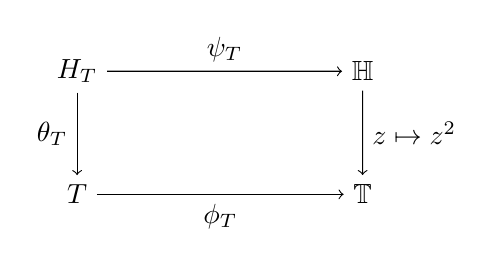
\begin{tikzpicture}[scale=1.25]
  \node (HT) at (0,1.25)  {$H_T$};
  \node (H)  at (2.9,1.25) {$\HH$};
  \node (T)  at (0,0)     {$T$};
  \node (TT) at (2.9,0)   {$\mathbb{T}$};
  \draw[->] (HT) -- node[above] {$\psi_T$} (H);
  \draw[->] (T)  -- node[below] {$\phi_T$} (TT);
  \draw[->] (HT) -- node[left]  {$\theta_T$} (T);
  \draw[->] (H)  -- node[right] {$z\mapsto z^2$} (TT);
\end{tikzpicture}
\end{center}

在 $\HH$ 中，我们取三条定向道路：
% [原文 p.151]
\[
\begin{array}{rcl}
p_k\colon(-1,1)&\to&\HH\\
t&\mapsto&t\,\ee^{2ik\pi/3},
\end{array}
\]
对 $k\in\{0,1,2\}$，并用映射 $z\mapsto z^2$ 投影每条道路。显然，这些道路满足覆叠 $\HH\to\mathbb{T}$ 的谱网络条件。

\Fig[0.78\linewidth]{figures/fig_13_10.png}{13.10}{覆叠 $\HH\to\mathbb{T}$。}

我们希望按下述方式沿边粘合六边形 $H_T$ 得到 $\Sigma$：设 $e$ 是 $\Delta$ 的一条边，它分隔两个三角形 $T_1$ 与 $T_2$。令 $\alpha_e\colon(0,1)\to e$ 为 $e$ 的参数化。由于 $\theta$ 在 $e$ 上不分歧，$\alpha_e$ 在 $\theta_{T_1}$ 下的提升由两条不相交的道路 $\alpha^1_{e_1},\alpha^1_{e_2}\colon(0,1)\to H_{T_1}$ 组成。我们假定提升 $\alpha^1_{e_1}$ 是相对于 $H_{T_1}$ 上的谱网络从汇（sink）走向源（source）的那条提升，而 $\alpha^1_{e_2}$ 是相对于 $H_{T_1}$ 上的谱网络从源走向汇的那条提升。对 $T_2$ 我们同样有 $\alpha^2_{e_1},\alpha^2_{e_2}\colon(0,1)\to H_{T_2}$。最后，我们通过把所有 $t\in(0,1)$ 的 $\alpha^1_{e_1}(t)$ 与 $\alpha^2_{e_1}(t)$ 等同、并把 $\alpha^1_{e_2}(t)$ 与 $\alpha^2_{e_2}(t)$ 等同，来粘合六边形 $H_{T_1}$ 与 $H_{T_2}$，见图 13.11。由这个粘合构造得到的空间是一个曲面，记作 $\Sigma$。映射 $\theta_T$ 给出带谱网络的分歧覆叠 $\theta\colon\Sigma\to S$。

\Fig[0.78\linewidth]{figures/fig_13_11.png}{13.11}{沿理想三角剖分 $\Delta$ 的边 $e$ 粘合。}

% [Tutor Note: 原文把 $\theta$ 写成 $\psi_T\circ(z\mapsto z^2)\circ\phi_T^{-1}$，但按交换图表，$\theta_T$ 应把 $H_T$ 送到 $T$，正确顺序为 $\theta_T=\phi_T^{-1}\circ(z\mapsto z^2)\circ\psi_T$：先用 $\psi_T$ 到 $\HH$，再平方到 $\mathbb{T}$，最后用 $\phi_T^{-1}$ 回到 $T$。原文写作逆序，属记号疏漏；以图表为准。]

% [原文 p.152]
\subsection{高阶谱网络}

本节中，我们将利用 Goncharov 与 Kontsevich 在 [168] 中引入的秩 $k\ge2$ 丛的谱覆盖的组合构造，来给出与该 $k$ 重分歧覆叠相关联的小谱网络的组合构造。这个构造产生一类非常特殊的谱网络，在 [156] 中称为\emph{极小谱网络}；不过这一类受限的谱网络在下文仍将非常重要，特别是因为它与 Fock--Goncharov 坐标的联系（见 §15.3）。我们先给出 [168] 中谱覆盖的构造。设 $S$ 为定向纤毛曲面，赋有理想三角剖分 $\Delta$。对任何整数 $k\ge2$，我们通过对 $S$ 的所有三角形 $t$ 粘合如图 13.12 所述的基本片段 $\Gamma_k^{(t)}$，定义 $S$ 上的\emph{二分图} $\Gamma_k$。

\Fig[0.85\linewidth]{figures/fig_13_12.png}{13.12}{限制在 $\Delta$ 的三角形 $t$ 上的图 $\Gamma_2^{(t)}$、$\Gamma_3^{(t)}$ 与 $\Gamma_4^{(t)}$。}

然后对每对共享三角剖分的一条边 $e$ 的三角形 $t$ 与 $t'$，我们在 $e$ 上把 $\Gamma_k^{(t)}$ 与 $\Gamma_k^{(t')}$ 相应的黑顶点等同；见图 13.13。白顶点是三价的，而黑顶点是单价的、二价的或三价的：单价与二价的黑顶点称为\emph{外部的}，三价的黑顶点称为\emph{内部的}。单价的黑顶点恰是 $\Gamma_k$ 落在 $S$ 边界上的顶点。

\Fig[0.48\linewidth]{figures/fig_13_13.png}{13.13}{对两个相邻三角形 $t$ 与 $t'$，$\Gamma_3^{(t)}$ 与 $\Gamma_3^{(t')}$ 的粘合。}

图 $\Gamma_k$ 嵌入 $S$ 中，故每个顶点从 $S$ 的定向继承其关联边上的循环次序。设 $\gamma=(v_1,\dots,v_r)$ 为
% [原文 p.153]
$\Gamma_k$ 上的一条道路，且 $1<i<k$。若边 $(v_{i-1},v_i)$ 与 $(v_i,v_{i+1})$（相应地 $(v_i,v_{i+1})$ 与 $(v_{i-1},v_i)$）按该次序在 $v_i$ 处依循环次序相邻，则说 $\gamma$ 在 $v_i$ 处\emph{左转}（相应地\emph{右转}）。由于图 $\Gamma_k$ 嵌入 $S$，$\Gamma_k$ 中的道路将与其在 $S$ 中的像等同。

$\Gamma_k$ 上的\emph{zig-zag 路径}（zig-zag path）是一条在每处白顶点右转、在每处黑顶点左转的道路 $(v_1,\dots,v_r)$。特别地，$\Gamma_k$ 的每条定向边恰好给出一条以该边开头的 zig-zag 路径。于是每条 zig-zag 路径都可以向两侧极大延拓。由于 $\Gamma_k$ 有限，一条 zig-zag 路径或者延拓为连接两个边界分支的道路，或者延拓为 $\Gamma_k$ 上的一个圈，而该圈的任何延拓都是周期的。以下我们假定所有 zig-zag 路径都是简单闭圈或连接边界分支的道路。

% [Tutor Note: 原文「$\Gamma_k$ 上的一条道路 $\gamma=(v_1,\dots,v_r)$，且 $1<i<k$」中上界应为 $r$（路径的顶点数），即 $1<i<r$；否则「$\gamma$ 在 $v_i$ 处左转/右转」中 $i$ 的取值范围将依赖于秩 $k$ 而与路径长度无关，显然不合定义。]

\begin{proposition}[13.16]
设 $\gamma$ 是 $\Gamma_k$ 上的 zig-zag 路径。则 $\gamma$ 在 $S$ 中的像或者同胚于一个圆周 $S^1$（其定向与 $S$ 的定向相符），或者同胚于一个闭区间，且 $S\setminus\gamma$ 有两个连通分支，其中一个是同胚于带一个穿孔的开圆盘或带一个边界穿孔的开半圆盘的连通分支。我们把这个特定的连通分支记作 $S_\gamma$，并把它内部的穿孔记作 $s_\gamma$。
\end{proposition}

设 $\gamma$ 是 $\Gamma_k$ 上的 zig-zag 路径，$\bar S_\gamma$ 是 $S_\gamma$ 在 $S$ 中的闭包。$S_\gamma$ 的边界是 $\gamma$ 在 $S$ 中的像，特别地它不含任何穿孔，因此 $\bar S_\gamma$ 同胚于带一个穿孔的闭（半）圆盘。

\begin{lemma}[13.17]
设 $k\ge2$。对 $S$ 的每个穿孔 $s$，$\Gamma_k$ 中恰有 $k$ 条 zig-zag 路径 $\gamma_s^{(1)},\dots,\gamma_s^{(k)}$，使得对一切 $1\le i\le k$ 有 $s=s_{\gamma_s^{(i)}}$。此外，对一切 $1\le i<j\le k$，有 $\gamma_s^{(i)}\subset S_{\gamma_s^{(j)}}$（图 13.14）。
\end{lemma}

\Fig[0.42\linewidth]{figures/fig_13_14.png}{13.14}{$\Gamma_3^{(t)}$ 中环绕穿孔 $s$ 的三条 zig-zag 路径 $\gamma_s^{(1)}$、$\gamma_s^{(2)}$ 与 $\gamma_s^{(3)}$。$t$ 在路径 $\gamma_s^{(i)}$ 上方的部分包含在 $S_{\gamma_s^{(i)}}$ 中。}

我们定义 $\Sigma_k$ 为把带穿孔的（半）圆盘粘到 $\Gamma_k$ 上所得的拓扑曲面：沿 $\Gamma_k$ 中每条 zig-zag 路径 $\gamma$，我们粘上一个 $\bar S_\gamma$ 的副本。我们如下定义 $\pi\colon\Sigma_k\to S$：$\Gamma_k$ 中一点的像是它在 $S$ 中的浸入像，而每个胞腔 $S_\gamma$
% [原文 p.154]
赋以由包含给出的映射 $S_\gamma\to S$。我们把 $\Sigma_k$ 中位于 $S_{\gamma_s^{(i)}}$ 内部的穿孔记作 $s_i$。

\begin{proposition}[13.18]
映射 $\pi\colon\Sigma_k\to S$ 是带简单分歧点的分歧 $k$ 重覆叠。分歧点恰是 $\Gamma_k$ 的内部黑顶点。
\end{proposition}

\begin{proof}
$\Gamma_k$ 的每条边都是恰好两条 zig-zag 路径的一部分，故 $\Sigma_k$ 在 $\Gamma_k$ 每条边内部的点附近以及在外部黑顶点附近都是拓扑曲面。每个白顶点恰是三条 zig-zag 路径边界上的点，每个胞腔 $S_\gamma$ 被粘到一对相邻的边上（见图 13.15）。于是白顶点的邻域是拓扑曲面。在所有这些情形中，我们也看出覆叠 $\pi$ 是正则的。在每个内部黑顶点的邻域中，$\Sigma_k$ 也是拓扑曲面，但覆叠 $\pi$ 在每个内部黑顶点处都是简单分歧的（见图 13.15）。
\end{proof}

\Fig[0.75\linewidth]{figures/fig_13_15.png}{13.15}{白顶点、内部黑顶点与外部黑顶点的邻域，以及这些顶点邻域中粘合的不同胞腔。}

\begin{remark}[13.19]
曲面 $\Sigma_2$ 与覆叠 $\pi\colon\Sigma_2\to S$ 同胚于 §13.5.1 中构造的那些。
\end{remark}

\Fig[0.85\linewidth]{figures/fig_13_16.png}{13.16}{$S$ 的一个三角形的 $3$ 重分歧覆叠。波浪蓝线是分支割线。}

我们现在可以构造与 $k$ 重分歧覆叠 $\pi\colon\Sigma_k\to S$ 相关联的 $\Sigma_k$ 上的小谱网络。为此，我们将描述 $S$ 的一个三角形的覆叠上的谱网络，而 $\Sigma_k$ 上的完整谱网络是所有三角形覆叠上的谱网络的并。首先注意，$S$ 的每个穿孔 $s$ 都是非分歧的，即 $|\pi^{-1}(s)|=k$。$s$ 的这 $k$ 条提升 $s_1,\dots,s_k$ 各自落在
% [原文 p.155]
引理 13.17 中定义的某个带穿孔圆盘 $S_{\gamma_s^{(i)}}$ 中，并继承由这些带穿孔圆盘的包含关系给出的次序 $s_1<\dots<s_k$。设 $t$ 是 $S$ 的一个三角形，$s$ 是该三角形的一个顶点，且 $2\le i\le k$。在 $S_{\gamma_s^{(i)}}\cap t$ 的边界上有 $k-i$ 个内部黑顶点，在 $S_{\gamma_s^{(i-1)}}\cap t$ 的边界上有 $k-i$ 个白顶点。这些黑顶点每一个都通过 $\Gamma_k^{(t)}$ 的一条边恰好连接到这些白顶点之一，且这些黑顶点是分歧点。在 $\Sigma_k$ 上，我们如下为这些黑顶点各定义一条谱网络的线：设 $v_b$ 是 $S_{\gamma_s^{(i)}}\cap t$ 边界上的一个内部黑顶点，$v_w$ 是 $S_{\gamma_s^{(i-1)}}\cap t$ 边界上与 $v_b$ 关联的白顶点。设 $p_1$ 是 $S_{\gamma_s^{(i)}}\cap t$ 中从 $s_i$ 到 $v_b$ 的一条道路，$p_2$ 是由沿图 $\Gamma_k^{(t)}$ 的边得到的从 $v_b$ 到 $v_w$ 的道路，$p_3$ 是 $S_{\gamma_s^{(i-1)}}\cap t$ 中从 $v_w$ 到 $s_{i-1}$ 的道路。谱网络的线就是拼接 $p_3.p_2.p_1$（$k=3$ 的情形见图 13.16 与图 13.17）。

\begin{proposition}[13.20]
如上构造的 $\Sigma_k$ 上所有道路构成的集合 $\mathcal{W}$ 是与 $k$ 重分歧覆叠 $\pi\colon\Sigma_k\to S$ 相关联的小谱网络。
\end{proposition}

\Fig[0.85\linewidth]{figures/fig_13_17.png}{13.17}{提升到 $\Sigma_3$ 的三角形上的小谱网络。谱网络诸线依其所经过的分支点而着以不同颜色。}

\begin{proof}
每条线 $p\colon[-1,1]\to\bar\Sigma_k$ 满足 $\pi(p(t))=\pi(p(-t))$（$t\in[-1,1]$），且 $\pi(p(-1))=\pi(p(1))$ 是 $\bar S$ 中的穿孔、$p(0)$ 是内部黑顶点，即分歧点。每个内部黑顶点属于三条 zig-zag 路径，因此位于三个形如 $S_{\gamma_s^{(i)}}$ 的胞腔的边界上。过每个黑顶点有三条 $\mathcal{W}$ 的线，方向交替（见图 13.18）。
% [原文 p.156]
$\Gamma_k$ 中与内部黑顶点相接的每条边恰好被 $\mathcal{W}$ 的一条线跟随，而与外部黑顶点相接的边不与 $\mathcal{W}$ 的任何线相交。在形如 $S_{\gamma_s^{(i)}}$ 的带穿孔圆盘内，$\mathcal{W}$ 的线之间没有相交；因此 $\mathcal{W}$ 的线之间（除分歧点处的相交外）的唯一相交都位于 $\Gamma_k$ 的白顶点上。这意味着所有这些相交都发生在已经越过其分歧点的线之间，故集合 $\mathcal{W}$ 是小谱网络。
\end{proof}

\Fig[0.40\linewidth]{figures/fig_13_18.png}{13.18}{谱网络三条线在内部黑顶点处的相交。}

\section{解析构造：WKB 谱网络}

现在设带穿孔的曲面 $S$ 按注 4.10 的意义赋有复结构，并考虑其紧化 $\bar S:=S\cup P$（参看 §4.3）。设 $\pi\colon T^*\bar S\to\bar S$ 为 $\bar S$ 上的全纯余切丛，其全纯结构由 $S$ 的复结构典范地诱导。考虑一个多元组 $\boldsymbol\phi:=(\phi_1,\dots,\phi_k)$，其中 $\phi_i$ 是 $(T^*\bar S)^{\otimes i}$ 的亚纯截面（对一切 $i\in\{1,\dots,k\}$），而 $P\subset\bar S$ 是 $\boldsymbol\phi$ 的所有极点构成的集合。

与 $\boldsymbol\phi$ 相关联的\emph{谱覆盖}定义为
\[
\Sigma_{\boldsymbol\phi}:=\Bigl\{\sum_{i=1}^{k}\phi_i y^{k-i}=0\ \Big|\ y\in T^*S\Bigr\}\subset T^*S,
\]
其中 $T^*S$ 是 $S$ 的余切丛。若把上面的截面 $\phi_i$ 取得足够一般，则覆叠 $\pi|_{\Sigma_{\boldsymbol\phi}}\colon\Sigma_{\boldsymbol\phi}\to S$ 是只有简单分歧的光滑分歧 $k$ 重覆叠。如前，令 $B$ 为 $S$ 中分支点的集合。

\begin{remark}[13.21]
为简便起见，我们将滥用记号，写作 $\pi\colon\Sigma_{\boldsymbol\phi}\to S$ 而不写 $\pi|_{\Sigma_{\boldsymbol\phi}}\colon\Sigma_{\boldsymbol\phi}\to S$。
\end{remark}

\begin{definition}[13.22]
若 $\Sigma_{\boldsymbol\phi}$ 光滑且只有简单分歧点，则称覆叠 $\pi\colon\Sigma_{\boldsymbol\phi}\to S$ 是\emph{简单的}。
\end{definition}

\begin{remark}[13.23]
当 $n=2$ 且 $\phi_1=0$ 时，$\Sigma_{\boldsymbol\phi}:=\{y^2+\phi_2=0\mid y\in T^*S\}$。特别地，$\Sigma_{\boldsymbol\phi}$ 简单当且仅当 $\phi_2$ 只有单零点。
\end{remark}

% [Tutor Note: 注 13.23 中的「$n=2$」应为「$k=2$」：本章一律用 $k$ 表示覆叠的次数，$n$ 未被用作秩；且结论 $y^2+\phi_2=0$ 正是 $k=2$ 时 $\sum_i\phi_i y^{k-i}=0$ 的形式。]

设如前 $\pi\colon\Sigma\to S$ 是只有简单分歧的光滑谱覆盖。我们定义空间
\[
\hat\Sigma:=\bigl\{(y,y')\in\Sigma\times\Sigma\ \big|\ \pi(y)=\pi(y'),\ y\neq y'\bigr\}\subset T^*S\times T^*S,
\]
称为覆叠 $\pi\colon\Sigma\to S$ 的\emph{根覆盖}（root covering）。它是 $S$ 的光滑 $(k^2-k)$ 叶分歧覆叠。存在自然的对合 $\mu\colon\hat\Sigma\to\hat\Sigma$，定义为 $\mu(y,y'):=(y',y)$，以及两个投影映射 $p_1,p_2\colon\hat\Sigma\to\Sigma$，分别满足 $p_1(x,y):=x$ 与 $p_2(x,y):=y$。显然 $p_1=p_2\circ\mu$ 且 $\pi\circ p_1=\pi\circ p_2:=\hat\pi$。

% [原文 p.157]
在根覆盖上存在自然的阿贝尔微分 $\rho$，定义如下：设 $\lambda$ 是 $T^*S$ 上的典范刘维尔（Liouville）$1$-形式。我们定义 $\rho:=p_1^*\lambda-p_2^*\lambda$，它在分歧点上方有零点。若取对应于 $\hat\Sigma$ 的定向叶状结构 $F_\rho$，则 $\mu$ 保持 $F_\rho$ 的叶，但反转定向，因为 $\mu^*\rho=-\rho$。

我们按以下两步，把与多元组 $\boldsymbol\phi$ 相关联的谱网络 $\mathcal{W}(\boldsymbol\phi)$ 构造为 $F_\rho$ 的一族叶：
\begin{enumerate}
\item $\rho$ 的临界图包含在 $\mathcal{W}(\boldsymbol\phi)$ 中；
\item 设 $\alpha_1,\alpha_2\colon(-1,1)\to\hat\Sigma$ 是 $\mathcal{W}(\boldsymbol\phi)$ 的两片叶，使得存在 $t_1,t_2\in(-1,1)$ 满足：$\alpha_1(t_1)$ 位于叶（sheet）$(i,j)$ 中，$\alpha_2(t_2)$ 位于叶 $(j,k)$ 中，且 $p_j(\alpha_1(t_1))=p_j(\alpha_2(t_2))$，即这两片叶到 $\Sigma$ 的投影在叶 $j$ 中相交。设 $p_0$ 为叶 $(i,k)$ 中的点，$p'_0$ 为叶 $(k,i)$ 中的点，使得 $\hat\pi(p_0)=\hat\pi(p'_0)=\hat\pi(\alpha_1(t_1))\in S$。然后我们向 $\mathcal{W}(\boldsymbol\phi)$ 添加 $F_\rho$ 的两片半叶：一片在叶 $(i,k)$ 中、从点 $p_0$ 出发且以 $p_0$ 为该叶的源；另一片在叶 $(k,i)$ 中、从点 $p'_0$ 出发且以 $p'_0$ 为该叶的汇；见图 13.19。
\end{enumerate}

\Fig[0.60\linewidth]{figures/fig_13_19.png}{13.19}{上文第 2 步所述的构造。}

% [原文 p.158]
上述构造 $\mathcal{W}(\boldsymbol\phi)$ 的过程一般地是无穷的，因为第二步中添加一片叶通常会产生新的叶在 $\Sigma$ 中投影后的相交。但有时该过程在有限多步后终止。在后一情形，$\mathcal{W}(\boldsymbol\phi)$ 投影到 $\Sigma$ 与 $S$ 后满足谱网络的条件。我们把对应于亚纯微分的谱网络称为 \emph{WKB 谱网络}。

\begin{example}[13.24]
若 $k=2$，则 $p_1$ 与 $p_2$ 是曲面的微分同胚。

若 $k=3$，则 $p_1\circ\pi\colon\hat\Sigma\to X$ 是 $6:1$ 分歧覆叠，$\pi\colon\Sigma\to X$ 是 $3:1$ 分歧覆叠，而 $p_i\colon\hat\Sigma\to\Sigma$（$i\in\{1,2\}$）是 $2:1$ 分歧覆叠。
\end{example}

% [Tutor Note: 例 13.24 中两处把底曲面写成 $X$（$p_1\circ\pi\colon\hat\Sigma\to X$、$\pi\colon\Sigma\to X$），而本章其余各处均记底曲面为 $S$；此处应为 $S$。它不影响三个次数的计算：$k=3$ 时 $|\hat\Sigma\to S|=k(k-1)=6$，$|\Sigma\to S|=3$，$|\hat\Sigma\to\Sigma|=2$。]

\begin{example}[13.25]
设 $\bar S=\C\PP^1$ 且 $k=3$。取 $\boldsymbol\phi=\ee^{\frac{i\pi}{2}}(0,-\dd z^2,z\,\dd z^3)$。$\boldsymbol\phi$ 的唯一极点是无穷远点，故 $S=\C\PP^1\setminus\{\infty\}=\C$。于是
\[
\Sigma=\bigl\{(z,y)\in T^*S\ \big|\ y^3-y+z=0\bigr\}.
\]
分支轨迹与判别式为零的点集一致：$\Delta(z)=4z^2-27=0$，由两个点组成。谱网络 $\mathcal{W}(\boldsymbol\phi)$ 就是图 13.9 中所示的那一个。
\end{example}

% [Tutor Note: 对 $y^3-y+z$，按判别式公式 $\Delta=-4a^3-27b^2$（$a=-1$，$b=z$）得 $\Delta(z)=4-27z^2$，零点为 $z=\pm2/(3\sqrt3)$。原文写 $\Delta(z)=4z^2-27$，相当于把系数次序写反（两种写法都恰有两个零点，故「由两个点组成」无误）。核对分支点位置时以 $4-27z^2$ 为准。]

\begin{remark}[13.26]
谱网络的更多例子见第 22 章，那里也讨论了 WKB 谱网络的物理实质。
\end{remark}

\begin{remark}[13.27]
所有秩 $2$ 的谱网络都同痕于一个 WKB 谱网络。反之，由于纤毛曲面上的二次微分定义一个理想三角剖分（见 §8.3），任何秩 $2$ 的 WKB 谱网络都具有 §13.5.1 中所述的形式。相反，对秩 $k\ge3$ 的谱网络，这两个论断都不成立：并非所有非退化谱网络都同痕于 WKB 谱网络，也并非所有 WKB 谱网络都具有 §13.5.2 中所述的形式。
\end{remark}

\section{用非退化谱网络作道路提升}

现在既然有了小谱网络的定义，我们就可以描述道路提升规则，它使后文能够构造非阿贝尔化映射。

% [原文 p.159]
设 $\pi\colon\Sigma\to S$ 为满足上述条件的分歧 $k$ 重覆叠，$\mathcal{W}$ 为 $\Sigma$ 上秩 $k$ 的小谱网络。我们希望构造一个映射 $\pi_1(S,p)\to\Z^{\mathrm{tw}}_B[\mathcal{P}(\Sigma)]$，其中 $p\in S$ 且 $p$ 不在 $\mathcal{W}$ 的任何线上。

我们考虑道路 $\gamma\colon[0,1]\to S$，其端点不在谱网络的任何线上，也不经过任何分支点。为把这条道路提升到 $\bar\Sigma$，我们把它分成若干片段 $\gamma=\gamma_n\cdot\ldots\cdot\gamma_1$，使每个 $\gamma_i$ 至多与谱网络 $\mathcal{W}$ 相交一次。这里我们用 $\cdot$ 表示道路的拼接，如路径代数的定义中那样。

若 $\gamma_i$ 不与谱网络相交，则按通常方式提升，得到 $\Sigma$ 中同样不与谱网络相交的 $k$ 条提升 $\gamma_i^{(1)},\dots,\gamma_i^{(k)}$。

若 $\gamma_i$ 与谱网络的线 $p_h$ 相交，则 $\gamma_i$ 只有两条标准提升在 $\Sigma$ 中与 $p_h$ 相交。这两条提升中的一条 $\gamma_i^{(j)}$ 在 $p_h$ 经过其分歧点\emph{之前}与 $p_h$ 相交，另一条 $\gamma_i^{(\ell)}$ 则在 $p_h$ 经过其分歧点\emph{之后}与之相交。在这种情形下，我们必须在标准提升之外再加一条新道路 $\gamma'_i$，如图 13.20。道路 $\gamma'_i$ 这样得到：沿 $\gamma_i^{(j)}$ 从其起点走到它与线 $p_h$ 的交点，然后沿 $p_h$（不穿过它）走到它与 $\gamma_i^{(\ell)}$ 相遇之处，再沿 $\gamma_i^{(\ell)}$ 走到其终点。

\Fig[0.65\linewidth]{figures/fig_13_20.png}{13.20}{用谱网络作道路提升。图为 $\Sigma$ 中（左）与 $S$ 中（右）的情形。}

\begin{definition}[13.28]
曲线 $\gamma$ 在 $\Sigma$ 中相对于谱网络 $\mathcal{W}$ 的\emph{提升} $\tilde\gamma$，是 $\gamma_i$ 的所有提升在 $\Z^{\mathrm{tw}}_B[\mathcal{P}(\Sigma)]$ 中的乘积：
\[
\tilde\gamma=\Bigl(\sum_{i=1}^{k}\gamma_1^{(i)}+\gamma'_1\Bigr)\cdot\ldots\cdot\Bigl(\sum_{i=1}^{k}\gamma_n^{(i)}+\gamma'_n\Bigr),
\]
其中对不与谱网络相交的片段 $\gamma_i$，令 $\gamma'_i=0$。
\end{definition}

% [Tutor Note: 定义 13.28 中求和号只作用于 $\gamma_1^{(i)}$，$\gamma'_1$ 在求和号外；若该片段不与 $\mathcal{W}$ 相交则取 $\gamma'_1=0$，此时括号化为 $\sum_{i=1}^k\gamma_1^{(i)}$。核对公式时注意 $n$ 是片段数、$k$ 是秩，两者不可混。]

\begin{theorem}[13.29]
这条道路提升规则是同伦不变的，即若两条道路 $\gamma$ 与 $\delta$ 相对于其端点同伦，则在 $\Z^{\mathrm{tw}}_B[\mathcal{P}(\Sigma)]$ 中 $\tilde\gamma=\tilde\delta$。
\end{theorem}

该定理是两个下述引理的推论：

\begin{lemma}[13.30]
设 $\gamma$ 是 $S$ 上的道路，它恰与谱网络的同一条线 $p_h$ 相交两次、且不与 $\mathcal{W}$ 的其他线相交，如图 13.21。则 $\tilde\gamma=\gamma^{(1)}+\dots+\gamma^{(k)}$，其中 $\gamma^{(1)},\dots,\gamma^{(k)}$ 是 $\gamma$ 到 $\Sigma$ 的 $k$ 条标准提升。
\end{lemma}

\begin{proof}
谱网络产生了另外两条提升 $\gamma'$ 与 $\gamma''$。这两条特殊提升在越过一个分歧点的意义下同伦，故在 $\Z^{\mathrm{tw}}_B[\mathcal{P}(\Sigma)]$ 中 $\gamma'+\gamma''=0$；见图 13.22。
\end{proof}

% [Tutor Note: $\gamma'+\gamma''=0$ 的机制：这两条额外提升只相差绕过分歧点的一个小环路 $\alpha_z^b$，而在扭转路径代数中由定义有 $\alpha_z^b=-e_z$，故 $\gamma'+\gamma''=0$；引理 13.31 证明中的 $\gamma'_1+\gamma'_5=0$ 等抵消同样归结为关系 $\alpha_z^b+e_z=0$。]

% [原文 p.160]
\Fig[0.40\linewidth]{figures/fig_13_21.png}{13.21}{与 $\mathcal{W}$ 的同一根线相交两次的环路。}

\Fig[0.72\linewidth]{figures/fig_13_22.png}{13.22}{$\gamma$ 的谱网络提升。}

\begin{lemma}[13.31]
设 $\gamma$ 是以 $m\in S$ 为基点的可缩环路，它绕 $S$ 中的分支点 $b$ 一圈，且恰与 $\mathcal{W}$ 从 $b$ 出发的三条线各相交一次，如图 13.23。则 $\tilde\gamma=e_{m_1}+\dots+e_{m_k}$，其中 $m_1,\dots,m_k$ 是 $m$ 到 $\Sigma$ 的 $k$ 条提升，而 $e_{m_i}$ 表示以 $m_i$ 为基点的平凡环路。
\end{lemma}

\Fig[0.40\linewidth]{figures/fig_13_23.png}{13.23}{绕分支点的小环路。}

\begin{proof}
对 $\gamma$ 应用谱网络提升规则，得到 $k+6$ 条道路：$k$ 条标准提升 $\gamma^{(1)},\dots,\gamma^{(k)}$（其中 $\gamma^{(j)}$ 与 $\gamma^{(\ell)}$ 如前与 $\mathcal{W}$ 相交），以及图 13.24 中所示的六条额外道路 $\gamma'_1,\dots,\gamma'_6$。在重新标号的意义下，我们假定 $\gamma^{(j)}$ 与 $\gamma^{(\ell)}$ 的端点为 $m_1$ 与 $m_2$。在 $\Z^{\mathrm{tw}}_B[\mathcal{P}(\Sigma)]$ 中有：
% [原文 p.161]
\[
\begin{aligned}
&\gamma^{(\ell)}+\gamma'_3=0,\\
&\gamma^{(j)}+\gamma'_6=0,\\
&\gamma'_1+\gamma'_5=0,\\
&\gamma'_4=e_{m_1},\\
&\gamma'_2=e_{m_2}.
\end{aligned}
\]
因此我们可以写
\[
\tilde\gamma=\sum_{i=1}^{k}\gamma^{(i)}+\gamma'_1+\gamma'_2+\gamma'_3+\gamma'_4+\gamma'_5+\gamma'_6=\sum_{i=1}^{k}e_{m_i}.
\]
\end{proof}

\Fig[0.68\linewidth]{figures/fig_13_24.png}{13.24}{由与谱网络相交而添加的全部六条道路，以及标准提升 $\gamma^{(j)}$ 与 $\gamma^{(\ell)}$。左上图中是与平凡道路同伦的道路，其余各图中是剩下的提升，它们按在 $\Z^{\mathrm{tw}}_B[\mathcal{P}(\Sigma)]$ 中相互抵消的道路对分组。}

% [原文 p.162]
\begin{exercise}
道路提升规则可以推广到非退化谱网络，并且它是同伦不变的。
\end{exercise}

我们给出如何提升一条与线 $p_h$（$h\in H_2$）相交的道路的提示。在图 13.25 中，我们用红色画出 $S$ 中正在被提升的曲线及它们在 $\Sigma$ 中的标准提升，并用蓝色画出额外的提升。

\Fig[0.78\linewidth]{figures/fig_13_25.png}{13.25}{沿关节的道路提升。}
}{}
\IfFileExists{part/ch14_15.tex}{% ============================================================
% 第 14 章  一般谱网络与 Fenchel–Nielsen 谱网络
% 第 15 章  非阿贝尔化与阿贝尔化
% 底本：Springer LNM 2386，Chapters 14–15，印刷 pp.163–180 / PDF p203–p220
% 交付：work/src/part/ch14_15.tex（片段，不含导言区）
% ============================================================

\chapter{一般谱网络与 Fenchel–Nielsen 谱网络}

% [原文 p.163]
\ChapterAbstract{本章研究更一般（退化）的谱网络，它们对许多物理应用都十分重要。这类一般网络的一个特殊类型出现在下述情形：某个 Strebel 微分的临界图的所有叶子的两端都落在分支点上。这样的谱网络称为 Fenchel–Nielsen 谱网络，因为它们与某些长度–扭转参数有关；这一构造将在 §15.6 中演示。}

\section{一般谱网络}

% [原文 p.163]
我们将把谱网络的定义作进一步的推广，以涵盖谱线相互重叠的情形，以及谱线终止于分支点而非穿孔的情形。这一层次的普遍性对第 IV 部分非常重要，但我们在此不描述它们的路径提升映射，因为一般情形下的构造在技术上更为复杂。关于路径提升映射的详细描述，我们参见 [210]。

设 $\pi\colon\overline{\Sigma}\to\overline{S}$ 是一个分歧的 $k$ 重覆叠。

\begin{definition}[14.1]
联系于 $\pi$ 的秩 $k$ 的\textbf{一般（或退化）谱网络}（general (or degenerate) spectral network）$\mathcal{W}$ 由 $\Sigma$ 上两族有限的光滑、简单、带定向的道路组成：
\[
\{p_h\colon[-1,1]\to\overline{\Sigma}\}_{h\in H_1}
\qquad\text{与}\qquad
\{p_h\colon[-1,1]\setminus\{0\}\to\overline{\Sigma}\}_{h\in H_2} ,
\]
其中 $H_1$ 与 $H_2$ 是两个不交的指标集。这些道路只能横截相交或者重叠，并且满足下列条件：
\begin{enumerate}[label=\arabic*.]
\item 对一切 $h\in H_1\cup H_2$ 与一切 $t\in(0,1]$，有 $\pi(p_h(t))=\pi(p_h(-t))$；
\item 对一切 $h\in H_1$，$\pi(p_h(0))\in B$ 是一个分支点；
\item 对一切 $h\in H_2$，下列极限存在：$p_h(+0):=\lim_{t\to+0}p_h(t)$ 与 $p_h(-0):=\lim_{t\to-0}p_h(t)$。此外 $p_h(+0)\neq p_h(-0)$，但 $\pi(p_h(+0))=\pi(p_h(-0))$；
\item 对一切 $h\in H_1\cup H_2$，$\pi(p_h(1))=\pi(p_h(-1))=s_j\in P$（对某个 $j$）是下列二者之一：
\begin{enumerate}[label=\alph*.]
\item 一个穿孔，此时相对于 $\pi^{-1}(s_j)$ 上的序有 $p_h(-1)<p_h(1)$；
% [原文 p.164]
\item 一个分歧点 $b'$，此时还存在一条经过 $b'$ 并与 $p_h$ 反向重叠的谱线 $p_{h'}$（见图 14.2）。这一对相互重叠的谱线称为\textbf{双墙}（double wall）或\textbf{双向街}（two-way street）；
\end{enumerate}
\item 任一分支点的邻域都如图 14.1 所示；
\item $\overline{\Sigma}$ 中不同的道路 $p_h$ 与 $p_{h'}$ 只能在一个点 $p_h(t)=p_{h'}(t')$ 处相遇，并且下列之一成立：
\begin{enumerate}[label=\alph*.]
\item $h,h'\in H_1$，$t=t'=0$，且 $p_h(t)=p_{h'}(t')$ 是一个分歧点；
\item $h,h'\in H_1\cup H_2$，$t,t'\in\{-1,1\}$，且 $p_h(t)=p_{h'}(t')$ 是一个穿孔；
\item $h,h'\in H_1\cup H_2$，$t\cdot t'>0$，此时我们还要求：除了与 $p_h$ 或 $p_{h'}$ 重叠的那条谱线之外，$\mathcal{W}$ 中没有任何谱线经过 $p_h(-t)$ 或 $p_{h'}(-t')$；
\item $h,h'\in H_1\cup H_2$，$t\cdot t'<0$，此时不妨设 $t<0$、$t'>0$。在这种情况下，存在一条谱线 $p_{h''}$，$h''\in H_2$，使得 $p_{h''}(+0)=p_h(-t)$ 且 $p_{h''}(-0)=p_{h'}(-t')$。此外，除了与 $p_h$、$p_{h'}$ 或 $p_{h''}$ 重叠的谱线之外，$\mathcal{W}$ 中没有任何其他谱线经过 $p_h(-t)$ 或 $p_{h'}(-t')$。
\end{enumerate}
\end{enumerate}
\end{definition}
% [Tutor Note: 原文条件 4a 引用 $\pi^{-1}(s_j)$ 上的一个序（“with respect to the order on $\pi^{-1}(s_j)$”），但前文从未定义该序；按上下文应理解为：在穿孔 $s_j$ 处取定一个小圆周（或取 $\Sigma\to S$ 在 $s_j$ 附近的局部模型），把 $\pi^{-1}(s_j)$ 的 $k$ 个点按该圆周上的循环顺序（等价地，按叶的编号）排成一个序，于是条件 4a 说的是谱线 $p_h$ 的终点 $p_h(1)$ 比起始点 $p_h(-1)$ “更靠后”，即谱线在 $\Sigma$ 上不封闭、而是从一叶绕到另一叶。核对方法：$k=2$ 且 $\pi^{-1}(s_j)=\{p_+,p_-\}$ 时该序只有两种取法，取反则 4a 的不等号同时反向，而“$p_h(-1)\neq p_h(1)$”这一实质内容不变；这说明原文所用的是一个任取的辅助序，不影响定义的实质。正文已按原文照译，未加解释性文字。]
% [Tutor Note: 条件 6 是“横截性 + 重叠相容性”的完备清单，用来排除三条以上谱线在同一内点相交的退化情形。其中 6c（$t\cdot t'>0$，两端参数同号）与 6d（$t\cdot t'<0$，异号）的区别在于两线在该点是否“同向”通过：同向时只允许另有与之重叠的谱线，异向时必须存在第三条谱线 $p_{h''}\in H_2$ 把两条半线接起来。核对方法：对一条双墙（$p_h$ 与 $p_{h'}$ 反向重叠）取交点处的参数，重叠意味着同一条几何道路被两个相反参数化，故 t 与 t' 异号，落在 6d；而 6c 处理的是两条真正不同方向的谱线恰好同向相切的情形。]

\Fig[0.55\linewidth]{figures/fig_14_1.png}{14.1}{$S$ 中一个分支点的邻域（左），以及 $\Sigma$ 中一个分歧点的邻域（右）。注意任一条谱线都可以成为双墙。}

与以往一样，我们记
\[
\mathcal{W}_\Sigma:=\bigcup_{h\in H_1\cup H_2}p_h\big((-1,1)\big)\subseteq\Sigma
\]
为 $\Sigma$ 上的谱网络，并记
\[
\mathcal{W}_S:=\pi(\mathcal{W}_\Sigma)\subseteq S
\]
为 $S$ 上的谱网络。

给定一个至少含有一条双墙的一般谱网络，我们称对每条双墙分别选取“英式”或“美式”为一个\textbf{消解}（resolution）。我们把这一选取理解为将双墙无穷小地劈开的方式，这一术语来自英国与美国的道路通行惯例。双墙的两种消解见图 14.2。当我们处理一般谱网络时，我们将始终假定已经作好了一个消解的选择。

\Fig[0.8\linewidth]{figures/fig_14_2.png}{14.2}{画在 $S$ 上的双墙的美式消解（左）与英式消解（右）。标号为 $ij$ 的谱线从 $\Sigma$ 的第 $i$ 叶走到第 $j$ 叶。注意按定义，双墙的每条谱线恰好经过两个分支点中的一个，另一个则是 $t\to\pm1$ 时的极限。}

% [原文 p.165]
\section{Fenchel–Nielsen 谱网络}

一般谱网络的定义允许谱线终止于分支点而非穿孔，只要它们是双墙即可。于是人们可以设想一个只有双墙、没有谱线终止于穿孔的谱网络。这样的谱网络甚至可以定义在闭曲面上，因为它不需要任何穿孔的存在。这样的谱网络确实存在，下面我们就来定义它们的一个特殊类型，称为 \textbf{Fenchel–Nielsen 谱网络}。这一类特殊的谱网络由 Hollands 与 Neitzke 在 [205] 中引入，之所以这样称呼，是因为这类谱网络与 §7.1 中定义的 Fenchel–Nielsen 坐标有很强的关联。这一关联将在 §15.6 中进一步研究。这些特殊的 WKB 谱网络出现在考虑 Strebel 微分（见 §8.5）的临界图之时。

设 $\overline{S}$ 是闭黎曼曲面，$P=\{s_1,\dots,s_n\}$ 是 $\overline{S}$ 上有限个标记点，$n\in\Z_{>0}$，令 $S=\overline{S}\setminus P$。设 $\omega$ 是 $\overline{S}$ 上的亚纯二次微分，在 $P$ 的各个点处有二阶极点。选取相位 $\vartheta\in\R/2\pi\Z$，使得 $\phi:=\ee^{-2\ii\vartheta}\omega$ 按定义 8.14 的意义是 Strebel 微分。这将意味着存在 $S$ 的一个裤子分解，使得 $\sqrt{\omega}$ 绕每条腿的周期具有相位 $\vartheta$。亚纯二次微分 $\omega$ 的平方根定义一个二重覆叠 $\pi\colon\Sigma_\omega\to S$，
\[
\Sigma_\omega:=\{(z,\lambda)\in S\times T_z^\ast S:\lambda^2=\omega(z)\} ,
\]
其中 $T_z^\ast S$ 是 $S$ 的余切丛在 $z$ 处的纤维。这里 $\pi(z,\lambda)=z$，而覆叠 $\pi\colon\Sigma\to S$ 的分支点是 $\omega$ 的零点。与 §13.6 中 WKB 谱网络的构造类似，我们把谱网络 $\mathcal{W}(\phi)$ 构造为临界图 $\hat{\mathcal{F}}_\phi$ 的一组叶，其中所有叶的两端都落在分支点上；于是每个叶给出网络 $\mathcal{W}(\phi)$ 的一条双墙。这样的谱网络称为 \textbf{Fenchel–Nielsen 谱网络}。

\begin{remark}[14.2]
把相位 $\vartheta$ 扰动为 $\vartheta_+=\vartheta+\epsilon$（相应地 $\vartheta_-=\vartheta-\epsilon$），其中 $\epsilon>0$ 充分小，则 $\phi$ 的临界叶分裂为两个正则叶，连接一个分支点%
% [原文 p.166]
与一个穿孔。当 $\epsilon\to0$ 时的极限便形成一条双墙，对应于 $\mathcal{W}(\phi)$ 的英式（相应地，美式）消解。
\end{remark}

$S\setminus\mathcal{W}(\phi)$ 的每个连通分支都是被闭的 $\vartheta$-轨道扫出的一个穿孔圆盘，而每个这样的分支的边界是由一条或多条\textbf{鞍连接}（saddle connection）构成的多边形。对每个这样的穿孔圆盘，Strebel 微分在穿孔 $s_j$（$j=1,\dots,n$）处的系数 $m_j\ee^{-\ii\vartheta}$，等价地，该穿孔圆盘中任一闭水平 $\vartheta$-轨道的长度，是一个正实数，它给 $S\setminus\mathcal{W}(\phi)$ 的每个连通分支打上标签。

一个 Fenchel–Nielsen 谱网络诱导出曲面 $S$ 的一个裤子分解，而在每条裤子上，该谱网络属于两种类型之一，[205] 中称它们为 \textbf{分子 I}（molecule I）与 \textbf{分子 II}（molecule II），见图 14.3。
% [Tutor Note: “每个分支都是被闭水平 $\vartheta$-轨道扫出的穿孔圆盘”可如下核对：在二阶极点 $s_j$ 处，$\phi$ 的标准局部形式为 $\phi\approx-\big(\frac{m_j}{2\pi}\big)^2\frac{\dd z^2}{z^2}$，其水平轨道是同心圆，故极点邻域内 $S\setminus\mathcal{W}(\phi)$ 的分支同胚于圆盘挖去极点；而两条临界叶（水平轨道的极限）给出该圆盘边界的两条边。于是边界多边形的每条边都是 $\phi$ 的一条鞍连接，即临界轨道的一段，其两端为分支点。]

\Fig[0.55\linewidth]{figures/fig_14_3.png}{14.3}{裤子上的两种可能的 Fenchel–Nielsen 谱网络：分子 I（上）与分子 II（下）。波浪线是分支割线，两个谱网络都采用英式消解。}

\begin{remark}[14.3]
对亚纯二次微分 $\omega$ 还存在另一种非一般的情形，此时可以构造出有趣的谱网络。即：可用同样的方式构造出一个同时含单墙与双墙的 WKB 谱网络。这样的谱网络称为\textbf{混合的}（mixed）；其实例可在 [205] 中找到，这些网络正是在该文中首次引入的。另一种有趣的%
% [原文 p.167]
谱网络情形同样由 [205] 引入，涉及所谓\textbf{收缩谱网络}（contracted spectral networks），它们是把一个 Fenchel–Nielsen 网络中的某些双墙塌缩到一起而得到的；换言之，是考虑某个圆环收缩到零尺寸时通常 Fenchel–Nielsen 谱网络的退化。
\end{remark}

% [原文 p.168]
% 本页为原书空白页（第 14 章章末的空页），无正文内容。

\chapter{非阿贝尔化与阿贝尔化}

% [原文 p.169]
\ChapterAbstract{作为迄今所引入谱网络的一个重要应用，本章给出非阿贝尔化映射与阿贝尔化映射的构造。这些映射刻画了黎曼曲面 $S$ 上秩 $n$ 丛的平坦联络，与谱曲线 $\Sigma$（$S$ 的 $n$ 叶分歧覆叠）上线丛的平坦联络之间的等价性。阿贝尔化后局部系统的单值（monodromy）正是簇 $\mathcal{X}$-坐标。因此（非）阿贝尔化的过程为在高阶泰希米勒空间的研究中使用谱网络提供了非常强的动机。特别地，我们展示如何用谱网络与阿贝尔化，在平坦联络的空间上诱导出 Fock–Goncharov 坐标或 Fenchel–Nielsen 坐标。论证谱网络与高阶泰希米勒理论之间联系的合适文献包括 [154]、[204]、[205]、[207]、[287]、[288]。}

\section{非退化谱网络的非阿贝尔化映射}

% [原文 p.169]
设 $S$ 是纤毛曲面，$\pi\colon\overline{\Sigma}\to\overline{S}$ 是带有非退化谱网络 $\mathcal{W}$ 的分歧 $k$ 重覆叠。与以往一样，$\pi$ 在 $\Sigma$ 上的分歧轨迹记作 $B'$，并记 $B:=\pi(B')\subset S$。设 $\mathcal{E}^{\mathrm{tw}}(\Sigma,\C^\times)$ 为 $\Sigma\setminus B'$ 上、在分歧点周围单值为 $-1$ 的平坦线丛所成的空间。

我们在空间 $\mathcal{E}^{\mathrm{tw}}(\Sigma,\C^\times)$ 中取一点，它给出 $\Sigma\setminus B'$ 上的一个线丛 $L\to\Sigma\setminus B'$，并带有平坦联络 $\nabla$。对 $q\in\Sigma\setminus B'$，我们用 $L_q$ 记 $L\to\Sigma\setminus B'$ 在 $q$ 上的纤维，它是一个一维的 $\C$-向量空间。

此外，我们固定 $p\in S\setminus\pi(\mathcal{W})$。我们如下构造一个表示 $\rho\colon\pi_1(S,p)\to\GL_k(\C)$。考虑如下 $k$ 维向量空间：
\[
V_p:=\bigoplus_{i=1}^{k}L_{p_i} ,
\]
% [原文 p.170]
其中 $\{p_1,\dots,p_k\}=\pi^{-1}(p)$。$V_p$ 有自然基，即 $(e_1,\dots,e_k)$，其中 $(e_i)$ 是 $L_{p_i}$ 的基，$i\in\{1,\dots,k\}$。

$S$ 上每个满足 $[\gamma]\in\pi_1(S,p)$ 的回路 $\gamma$ 都可以关于谱网络 $\mathcal{W}$ 提升到 $\Sigma$。于是我们得到一个元素 $x\in\mathbb{Z}^{\mathrm{tw}}_{B'}[\mathcal{P}(\Sigma)]$，按构造它是 $\Sigma$ 上曲线 $\gamma_r$（$r\in I$，$I$ 为有限指标集）的有限和，使得
\begin{equation}
\gamma_r(0),\gamma_r(1)\in\pi^{-1}(p) , \tag{15.1}
\end{equation}
且 $x=\sum_{r\in I}\gamma_r$。我们考虑向量 $w=\sum_{i=1}^{k}a_ie_i\in V_p$，$i\in\{1,\dots,k\}$。由于 (15.1)，沿 $\gamma$ 的平行移动可以定义为
\[
T_\gamma:=\sum_{r\in I}T_{\gamma_r}\in\bigoplus_{\tilde p,\tilde q\in\pi^{-1}(p)}L(E_{\tilde p},E_{\tilde q}) ,
\]
其中 $T_{\gamma_r}$ 是沿 $\gamma_r$ 的平行移动，由 $\Sigma$ 上的联络 $\nabla$ 给出。

对每个满足 $\gamma_r(0)=p_i$、$\gamma_r(1)=p_j$ 的 $\gamma_r$（$i,j\in\{1,\dots,k\}$），我们可以考虑 $T_{\gamma_r}e_i=t_re_j\in E_{p_j}$。我们可以按如下法则把 $T_{\gamma_r}$ 扩充为 $V_p$ 上的线性映射：
\[
T_{\gamma_r}e_l=
\begin{cases}
t_re_j, & l=i\\
0, & l\neq i .
\end{cases}
\]
我们按法则 $T_\gamma:=\sum_{r\in I}T_{\gamma_r}$ 定义线性映射 $T_\gamma\colon V_p\to V_p$。按构造，这个映射是线性的；并且由于借助谱网络 $\mathcal{W}$ 的路径提升是同伦不变的，而 $\Sigma$ 上的联络是平坦的，映射 $T_\gamma$ 只依赖于 $\gamma$ 在 $\pi_1(S,p)$ 中的同伦类。
% [Tutor Note: 式 (15.1) 之所以关键，是因为它保证每个 $\gamma_r$ 的两端都落在同一纤维 $\pi^{-1}(p)$ 上，于是 $T_{\gamma_r}$ 是 $L$ 的各纤维之间的同构，可以相加而得到 $V_p$ 上的线性映射；否则 $T_\gamma$ 无法定义。另注：原文在紧接本页之处写 “T_γ := Σ_{r∈I} T_{γ_k}”，其中下标 $k$ 应为 $r$——求和指标是 $r\in I$，且同段上文已写 $T_{\gamma_r}$；这是原文的笔误，正确形式为 $T_\gamma=\sum_{r\in I}T_{\gamma_r}$。]

于是我们得到一个映射 $\rho\colon\pi_1(S,p)\to\Aut(V_p)$，它是群同态。把 $\Aut(V_p)$ 与 $\GL_k(\C)$ 作一个等同之后，我们得到空间 $\mathcal{E}(S,\GL_k(\C))$ 中的一个元素。$\mathcal{E}^{\mathrm{tw}}(\Sigma,\C^\times)$ 的每个元素，连同覆叠 $\pi\colon\Sigma\to S$ 以及联系于 $\pi$ 的谱网络 $\mathcal{W}$，都给出空间 $\mathcal{E}(S,\GL_k(\C))$ 中的一个元素：
\[
\pi_1(S,p)\xrightarrow[\text{network}]{\text{spectral}}\mathbb{Z}^{\mathrm{tw}}_{B'}[\mathcal{P}(\Sigma)]\xrightarrow[\text{on }\Sigma]{\text{connection}}\GL_k(\C) .
\]

我们就这样构造出了一个映射 $\mathcal{E}^{\mathrm{tw}}(\Sigma,\C^\times)\to\mathcal{E}(S,\GL_k(\C))$。此外，所得到的 $\GL_k(\C)$-局部系统容许一个自然的标架（framing），由
\[
F(p):=\big(L_{p_1},\,L_{p_1}\oplus L_{p_2},\,\dots,\,L_{p_1}\oplus\cdots\oplus L_{p_k}\big)
\]
给出；于是我们得到映射 $\mathcal{E}^{\mathrm{tw}}(\Sigma,\C^\times)\to\mathcal{E}^{\mathrm{fr}}(S,\GL_k(\C))$。要说明这确实是一个非阿贝尔化映射，我们需要验证它覆盖 $\mathcal{E}^{\mathrm{fr}}(S,\GL_k(\C))$ 的一个开稠密子集。在下一节中，我们对于适应 $S$ 的理想三角剖分的谱网络证明这一点。

\section{非退化谱网络的阿贝尔化映射}

\subsection{秩二}

% [原文 p.171]
与以往一样，设 $S$ 是纤毛曲面。我们在 $S$ 上固定一个理想三角剖分 $\Delta$，并设 $\pi\colon\overline{\Sigma}\to\overline{S}$ 是由 $\Delta$ 连同谱网络 $\mathcal{W}$ 构造出的分歧 $2:1$ 覆叠。

我们取 $\mathcal{E}^{\mathrm{fr}}_\Delta(S,\GL_2(\C))$ 的一个元素，再次把它看作一个带标架的秩 $2$ 平坦向量丛 $(V,\nabla)$，即：对每个穿孔 $p$ 及其一个（可缩到 $p$ 的）小邻域 $U_p$，存在 $V$ 的一个 $\nabla$-不变线子丛 $\ell_p$。由 §10.2.2 中定义的 $\Delta$-横截性，对由 $\Delta$ 的一条边相连的两个穿孔，其 $\nabla$-不变线丛（沿该边搬运到某个公共点）处于直和之中。

\begin{remark}[15.1]
到 $\GL_2(\C)$ 的表示可能不容许任何 $\Delta$-横截的标架。例如，对于来自通过上三角矩阵群分解的表示的联络，这一性质不成立。不过，容许 $\Delta$-横截标架的联络是一般的（generic），即它们构成 $\mathcal{E}(S,\GL_2(\C))$ 的一个开稠密子集。
\end{remark}

现在取 $S\setminus\pi(\mathcal{W})$ 的一个连通分支 $C$，称为一个\textbf{胞腔}（cell，见图 15.1（右））。$C$ 是一个四边形，$C$ 的两个顶点是分支点，另外两个顶点是穿孔，设为 $p_1$ 与 $p_2$。由于 $C$ 单连通，我们可以取任意点 $z\in C$，并把 $\nabla$-不变子丛 $\ell_1:=\ell_{p_1}$ 与 $\ell_2:=\ell_{p_2}$ 从邻域 $U_{p_1}$ 与 $U_{p_2}$ 搬运到 $z$。由于 $C$ 单连通，这一平行移动不依赖于道路的选取。

\Fig[0.8\linewidth]{figures/fig_15_1.png}{15.1}{$\Sigma$ 中与 $S$ 中的胞腔。}

$C$ 关于 $\pi$ 的提升由 $C$ 的两个不交的拷贝 $C_1$ 与 $C_2$ 组成（见图 15.1（左））。我们假定 $C_1$ 含 $p_1$ 的提升，它是一个汇点（sink）；$C_2$ 含 $p_2$ 的提升，它是一个汇点。我们定义线丛 $L$：在 $C_1$ 上为 $\ell_1$，在 $C_2$ 上为 $\ell_2$。

为了整体地构造 $L$，我们需要沿谱网络的谱线把 $L$ 粘合起来，且粘合方式保持平行移动。为此，我们取两个共%
% [原文 p.172]
享 $\mathcal{W}$ 的一条边 $w$ 的胞腔 $C$ 与 $C'$。于是 $C$ 与 $C'$ 共享一个穿孔；不妨设它是 $p_2$。$C'$ 的第二个穿孔记作 $p'_2$。$C'$ 上相应的 $\nabla$-不变线丛记作 $\ell'_1$（对应于 $p_1$）与 $\ell'_2$（对应于 $p'_2$）。我们在 $C$ 上取 $\ell_1$ 与 $\ell_2$ 的截面 $s_1$ 与 $s_2$，在 $C'$ 上取 $\ell'_1$ 与 $\ell'_2$ 的截面 $s'_1$ 与 $s'_2$。我们可以假定 $s_1$ 在 $w$ 的一个邻域 $U_w$ 中与 $s'_1$ 一致，且 $s'_2(z)=s_2(z)+\alpha(z)s_1(z)$，其中 $\alpha\colon U_w\to\C$ 是某个函数。

现在设 $\nabla s_i=\de_is_i$、$\nabla s'_i=\de'_is_i$ 在 $U_w$ 中成立，其中 $\de_1,\de_2,\de'_1,\de'_2$ 是某些 $1$-形式。我们沿 $U_w$ 把 $L|_C$ 与 $L|_{C'}$ 粘合起来，把 $s_i$ 与 $s'_i$ 等同（$i\in\{1,2\}$）。这一粘合保持平行移动，当且仅当 $\de_1=\de'_1$ 且 $\de_2=\de'_2$。由于 $s_1=s'_1$ 在 $U_w$ 中成立，故 $\de_1=\de'_1$。进一步，一方面
\[
\nabla s'_2=\nabla(s_2+\alpha s_1)=\nabla s_2+\de\alpha\cdot s_1+\alpha\nabla s_1=\de_2s_2+\de\alpha\cdot s_1+\alpha \de_1s_1 .
\]
另一方面 $\nabla s'_2=\de'_2s'_2=\de'_2s_2+\de'_2\alpha s_1$。由于 $s_1$ 与 $s_2$ 线性无关，故 $\de_2=\de'_2$。因此，按这种方式我们可以构造 $\Sigma\setminus B'$ 上的一个平坦线丛，它在 $B'$ 的点周围单值为 $-1$，从而给出 $\mathcal{E}^{\mathrm{tw}}(\Sigma,\C^\times)$ 的一个元素。直接计算表明，这一过程是 §15.1 的非阿贝尔化过程的逆过程。
% [Tutor Note: 比较 $\nabla s'_2$ 的两种展开时，应分别比较 $s_2$ 与 $s_1$ 的系数：$s_2$ 的系数给出 $\de_2=\de'_2$（原文采用了这一步）；$s_1$ 的系数给出 $\de\alpha+\alpha \de_1=\de'_2\alpha$，即 $\de\alpha=\alpha(\de_2-\de_1)$，这正是联络 $1$-形式在标架变换 $s'_2=s_2+\alpha s_1$ 下的标准变换律（对 $\de_1=\de'_1$ 的情形）。核对方法：把 $\nabla$ 在标架 $(s_1,s_2)$ 下写成矩阵 $\de+\diag(\de_1,\de_2)$，在标架 $(s_1,s'_2)$ 下写成 $\de+\diag(\de_1,\de'_2)$，用 (3.4) 式比较即得同一结论。]

\subsection{高阶}

设 $S$ 是纤毛曲面，$\Delta$ 是 $S$ 的理想三角剖分。设 $k\ge2$。设 $\pi\colon\Sigma_k\to S$ 是 §13.5.2 中构造的分歧 $k$ 重覆叠。设 $(V,\nabla,F)\in\mathcal{E}^{\mathrm{fr}}_\Delta(S,\GL_k(\C))$。我们再次有一个 $(V,\nabla)$ 的标架 $F$，即在每个穿孔 $p$ 的小邻域中，$V$ 的平坦子丛的一个嵌套序列
\[
F^p_0\subset F^p_1\subset\cdots\subset F^p_n ,
\]
其中对一切 $1\le i\le n-1$ 有 $\dim F^p_i=i$。

设 $t$ 是 $\Delta$ 的一个三角形，$(p,q,r)$ 是 $t$ 的各顶点处的穿孔。由于 $t$ 单连通，我们可以用 $\nabla$ 把三个旗子丛 $F^p$、$F^q$ 与 $F^r$ 搬运到 $t$ 中任一公共点。回忆一下：由于 $\nabla$ 是 $\Delta$-横截的，对任意三个满足 $a+b+c=k$ 的非负整数 $a,b,c$，都有
\[
F^p_a\oplus F^q_b\oplus F^r_c=V .
\]
特别地，这一假设保证：对任意三个满足 $a+b+c=2k+1$ 的非负整数 $a,b,c$，从 $F^p_a\cap F^q_b\cap F^r_c$ 到 $F^p_a/F^p_{a-1}$（相应地 $F^q_b/F^q_{b-1}$ 与 $F^r_c/F^r_{c-1}$）的典范投影是同构。

\begin{remark}[15.2]
容许 $\Delta$-横截标架的联络所成的子集在 $\mathcal{E}(S,\GL_k(\C))$ 中是开稠密的。
\end{remark}

我们如下在 $\Sigma_k$ 上构造线丛 $L$。设 $p$ 是 $S$ 的一个穿孔，$1\le a\le n$。设 $S_{\gamma_p^{(a)}}$ 是引理 13.17 中定义的穿孔圆盘。在这个穿孔圆盘上，线丛 $L$ 是平凡丛 $F^p_a/F^p_{a-1}$。设 $e$ 是 $\Gamma_k$ 的一条边，$t=(p,q,r)$ 是含 $e$ 的三角形。沿 $e$ 恰好粘合着 $\Sigma_k$ 中的两个穿孔圆盘。设 $S_{\gamma_p^{(a)}}$ 与 $S_{\gamma_q^{(b)}}$ 是这两个圆盘。在这些圆盘内部，线丛 $L$ 分别是 $F^p_a/F^p_{a-1}$ 与 $F^q_b/F^q_{b-1}$。它们沿 $e$ 通过同构
% [原文 p.173]
\[
F^p_a/F^p_{a-1}\cong F^p_a\cap F^q_b\cap F^r_{2k+1-a-b}\cong F^q_b/F^q_{b-1}
\]
粘合起来。$L$ 的这一构造具有局部常值的转移函数，故它定义了 $\Sigma_k$ 去掉 $\Gamma_k$ 的顶点之后的一个平坦线丛 $L$。一个简单的线性代数计算表明：$L$ 绕 $\Gamma_k$ 的白顶点的单值是平凡的，而绕内部黑顶点（即 $\pi\colon\Sigma_k\to S$ 的分歧轨迹）的单值是 $-1$。我们就这样构造出了 $\mathcal{E}^{\mathrm{tw}}(\Sigma,\C^\times)$ 的一个元素。再次，直接计算表明 $L$ 的非阿贝尔化是 $(V,\nabla)$。

\section{谱网络与 Fock–Goncharov 坐标}

设 $S$ 是纤毛曲面，$\Delta$ 是 $S$ 的理想三角剖分。非阿贝尔化映射与阿贝尔化映射定义了 $S$ 上秩 $k$ 的 $\Delta$-横截带标架平坦向量丛的模空间 $\mathcal{E}^{\mathrm{fr}}_\Delta(S,\GL_k(\C))$ 与 $\Sigma_k$ 上在分歧点周围单值为 $-1$ 的平坦线丛的模空间 $\mathcal{E}^{\mathrm{tw}}(\Sigma_k,\C^\times)$ 之间的一个同胚。后一个模空间要容易研究得多：它没有标架（因而没有横截性条件），并且线丛的空间容许一个非常方便的参量化，即作为第一同调群 $H_1(\Sigma_k)$ 的特征所成的集合（见注 3.31 与例 13.1）。特别地，空间 $\mathcal{E}(\Sigma_k,\C^\times)$ 同胚于 $(\C^\times)^n$，其中 $n$ 是 $H_1(\Sigma_k)$ 的维数。这一同胚由 $H_1(\Sigma_k)$ 的一组基的选取给出，而我们可以把这组基取为 $\Sigma_k$ 上 $n$ 条曲线的一个集合。这 $n$ 条曲线的和乐的选取随即唯一确定 $\Sigma_k$ 上的一个平坦线丛，从而通过非阿贝尔化映射确定 $S$ 上一个秩 $k$ 的 $\Delta$-横截带标架平坦向量丛。这并不是我们第一次参量化 $\mathcal{E}^{\mathrm{fr}}_\Delta(S,\GL_k(\C))$；在 §10.2.3 中我们已经用 Fock–Goncharov 坐标描述过这个空间的一种参量化。本节的目标是要说明：对谱曲面 $\Sigma_k$ 与 $H_1(\Sigma_k)$ 的基作适当选取之后，这两种参量化是相同的：每个 Fock–Goncharov 坐标对应于 $\Sigma_k$ 上某条特定曲线的和乐，而所有这些曲线的集合构成 $H_1(\Sigma_k)$ 的一组基。

谱网络与 Fock–Goncharov 坐标之间的关系由 Gaiotto、Moore 与 Neitzke 在 [156] 中作了研究。在该文中，他们利用底曲面 $S$ 上一个经过恰当选取的谱网络之补集的连通分支，与联系于带标架表示 $(V,\nabla,F)$ 的 snakes（见 §10.2.4 的讨论）之间的一个对应，来说明：阿贝尔化局部系统绕谱覆盖上特定曲线的单值正是 $V$ 的 $\mathcal{X}$-坐标。我们这里采取的方法略有不同，这源于我们构造阿贝尔化映射的方式。

我们首先关注三个横截旗的情形，即 $S$ 是带有穿孔 $p,q,r$ 的理想三角形。设 $n\ge2$，$(A,B,C)$ 是 $\C^n$ 中三个横截旗。如 §10.2.3 中所讨论，这三个旗由 $\frac{(n-1)(n-2)}{2}$ 个三重比的数据所决定，这些三重比称为该三元组的 $\mathcal{X}$-坐标。在 §13.5.2 中，我们构造了 $S$ 的 $k$ 重谱覆盖 $\Sigma_k$ 连同
% [原文 p.174]
$\Sigma_k$ 上的谱网络 $\mathcal{W}$。以三个旗 $(A,B,C)$ 为标架的 $S$ 上平凡局部系统于是可以被阿贝尔化为 $\Sigma_k$ 上的平坦线丛 $L$。当 $n$ 为偶数时曲面 $\Sigma_k$ 有 $\frac{n}{2}$ 个边界分支，当 $n$ 为奇数时有 $\frac{n+1}{2}$ 个边界分支；而 $\Sigma_k$ 上有 $\frac{n(n-1)}{2}$ 个简单分歧点。由 Riemann–Hurwitz 公式，当 $n$ 为偶数时 $\Sigma_k$ 的亏格为 $\frac{(n-2)^2}{4}$，当 $n$ 为奇数时为 $\frac{(n-1)(n-3)}{4}$。

在两种情形下，第一同调群 $H_1(\Sigma_k)$ 的维数（它同时也是 $\Sigma_k$ 上平坦线丛的模空间的维数）都是 $\frac{(n-1)(n-2)}{2}$。沿用 §13.5.2 的记号，设 $a,b,c\ge0$ 满足 $a+b+c=2k+3$，并设 $v_{a-1,b,c}$（相应地 $v_{a,b-1,c}$、$v_{a,b,c-1}$）是 $\Gamma_k$ 中位于交集 $\gamma_p^{(a-1)}\cap\gamma_q^{(b)}\cap\gamma_r^{(c)}$（相应地 $\gamma_p^{(a)}\cap\gamma_q^{(b-1)}\cap\gamma_r^{(c)}$、$\gamma_p^{(a)}\cap\gamma_q^{(b)}\cap\gamma_r^{(c-1)}$）上的黑顶点。设 $\tilde{x}_{a,b,c}$ 是 $S$ 上绕这三个分歧点的回路（见图 15.2）。
% [Tutor Note: 这里的维数 $\frac{(n-1)(n-2)}{2}$ 与前一段“三个横截旗由 $\frac{(n-1)(n-2)}{2}$ 个三重比决定”中的数目完全一致，这正是本节论证的关键一致性：$\mathcal{X}$-坐标的个数必须等于 $H_1(\Sigma_k)$ 的秩，否则“每个 $\mathcal{X}$-坐标对应一条基曲线的和乐”这一陈述无法成立。核对方法：取 $n=2$ 得 $0$，与 $\Sigma_2$ 上只有平凡同调一致（此时三个旗的模空间是零维的）；取 $n=3$ 得 $1$，此时恰有一个三重比。]

\Fig[0.5\linewidth]{figures/fig_15_2.png}{15.2}{联系于 $\Gamma_4$ 的道路 $\tilde{x}_{3,4,4}$。分歧点（即内部黑顶点）用蓝色叉号表示。}

把道路 $\tilde{x}_{a,b,c}$ 提升到 $\Sigma_k$（用标准的路径提升法则，而非谱网络法则），我们得到 $k$ 个不同的提升，其中 $k-2$ 个是 $\Sigma_k$ 中的闭回路，另外两个不是回路，但衔接起来之后构成一个回路。我们用 $x_{a,b,c}$ 记衔接这两个提升所得的回路。下述命题可由阿贝尔化局部系统 $L$ 的定义与三重比的定义推出：

\begin{proposition}[15.3]
$L$ 沿 $x_{a,b,c}$ 的单值等于三重比 $r_{a,b,c}(F(p),F(q),F(r))$。
\end{proposition}

现在考虑共享一条以 $p$ 与 $q$ 为端点的边的两个三角形 $t_1$ 与 $t_2$。设 $r$ 与 $s$ 是其余两个穿孔，使得 $t_1=(p,q,r)$ 且 $t_2=(p,s,q)$，并设 $(F(p),F(s),F(q),F(r))$ 是 $S=t_1\cup t_2$ 上平凡局部系统的一个横截标架。设 $\Gamma_k$ 是 §13.5.2 中在 $S$ 上构造的图。对满足 $a+b=k+2$ 的 $a,b\ge0$，设 $\tilde{x}_{a,b}$ 是绕两个内部黑顶点 $v^{(t_1)}_{a,b,n}$ 与 $v^{(t_2)}_{a,n,b}$ 的回路，如图 15.3 所示。

再次，$\tilde{x}_{a,b}$ 到 $\Sigma_k$ 有 $k$ 个标准提升，其中恰好两个不是可缩回路。我们在 $\Sigma_k$ 上选取其中一个提升 $x_{a,b}$。由我们对 $\Sigma_k$ 上阿贝尔化局部系统 $L$ 的构造，我们有下述命题：

\Fig[0.65\linewidth]{figures/fig_15_3.png}{15.3}{联系于 $\Gamma_4$ 的道路 $\tilde{x}_{2,4}$。分歧点（即内部黑顶点）用蓝色叉号表示。}

% [原文 p.175]
\begin{proposition}[15.4]
$L$ 沿 $x_{a,b}$ 的单值等于交比 $r_{a,b}(F(p),F(s),F(q),F(r))$。
\end{proposition}

通过对谱覆盖 $\Sigma_k$ 的拓扑作仔细研究，可以证明：取遍所有可能的回路 $x_{a,b,c}$ 与 $x_{a,b}$ 所得的族构成 $H_1(\Sigma_k)$ 的一组基。因此，Fock–Goncharov 坐标恰好就是绕谱曲面 $\Sigma_k$ 的第一同调群的一组基的单值。

\begin{remark}[15.5]
这一对应是就谱曲面 $\Sigma_k$ 的这一特定选取而言的。一般说来，把 Fock–Goncharov 坐标与在另一个谱曲面上的阿贝尔化的和乐联系起来并不容易。其他簇变量是否容许类似的几何描述，目前也尚不清楚。
\end{remark}

\begin{remark}[15.6]
在 [156] 中，Gaiotto、Moore 与 Neitzke 证明了：当 $k\le5$ 时，谱曲面 $\Sigma_k$ 及其谱网络按 §13.6 的意义是 WKB 谱网络。这一结论猜想对 $k>5$ 仍然成立。他们还证明，这些谱网络可以通过对 Argyres–Douglas 理论 $AD_1$ 的“第 $k$ 层提升”（level $k$ lift）作扰动而得到。
\end{remark}

\section{Fenchel–Nielsen 谱网络的阿贝尔化映射}

我们将构造联系于闭曲面 $S$ 上一个 Fenchel–Nielsen 谱网络 $\mathcal{W}$（带选定的美式或英式消解）的阿贝尔化映射。我们采用与 §15.2.1 中秩二非退化网络所给出的方法非常类似的做法。与非退化情形一样，除了 $S$ 上平坦 $\GL_2$-丛的数据之外，我们还需要一些额外数据，我们像对非闭曲面那样称之为标架。为此我们注意：$\mathcal{W}$ 在 $S$ 中的补集是有限多个连通分支的不交并，每个分支都同胚于圆环；而其中任一分支 $C$ 到 $\Sigma$ 的提升，是两个圆环 $C_1,C_2\subset\Sigma$ 的不交并。
% [Tutor Note: 这里“每个分支同胚于圆环”是 Fenchel–Nielsen 网络的标志性特征，可与 §14.2 对照核对：非退化网络的补集分支是胞腔（四边形），因为谱线终止于穿孔；而 FN 网络的谱线全是双墙、没有穿孔端点，故补集分支沿对偶方向是无孔的，只能是圆环。核对方法：由 §14.2，$S\setminus\mathcal{W}(\phi)$ 的每个分支是被闭 $\vartheta$-轨道扫出的穿孔圆盘；而在闭曲面情形（$P=\varnothing$ 的退化极限）这些圆盘两两粘合成圆环。]

% [原文 p.176]
我们利用谱网络的消解来对 $C$ 的定向作一个选取：$C_1$ 或 $C_2$ 中之一的边界由谱线的前半段构成，即某些谱线 $p_h\in\mathcal{W}$ 的像 $p_h\big((-1,0]\big)$。至多重新命名之后，我们把该提升称为 $C_1$，并按谱线在 $C_1$ 边界上诱导的定向来定向 $C$。我们称 $C$ 的这一方向为\textbf{正}（或 $+$）向，而相反方向为\textbf{负}（或 $-$）向。

\begin{definition}[15.7]
设 $V\in\mathcal{E}(S,\GL_2(\C))$ 是 $S$ 上的平坦 $\GL_2(\C)$-丛。$V$ 的一个\textbf{标架}是对每个这样的定向圆环 $C$，选取 $V$ 绕 $C$ 沿 $+$ 方向的单值 $M_+$ 的一条特征线 $\ell_+(C)$，以及沿 $-$ 方向的单值 $M_-=M_+^{-1}$ 的一条特征线 $\ell_-(C)$。我们要求 $\ell_+\neq\ell_-$，并且联系于一条双墙两侧的标架是横截的。
\end{definition}

\begin{remark}[15.8]
为使平坦 $\GL_2(\C)$-丛容许一个标架，绕每个圆环的单值必须是可对角化的。当相应的表示是 Fuchs 型时尤其如此，因为此时绕每条闭曲线的单值都是 $\SL_2(\C)$ 中的双曲元素。
\end{remark}
% [Tutor Note: $\ell_-(C)$ 取作 $M_-=M_+^{-1}$ 的特征线而非 $M_+$ 的另一条特征线，是必须的：$C$ 的 $-$ 向与 $+$ 向是同一条圆环上方向相反的两条曲线，故其单值互为逆（同伦类取逆）。核对方法：若 $M_+$ 有特征值 $\lambda,\lambda^{-1}$（$\GL_2$ 情形下 $\det M_+$ 未必为 $1$，则记特征值为 $\lambda,\mu$），则 $M_-=M_+^{-1}$ 的特征值为 $\lambda^{-1},\mu^{-1}$，特征线相同但标注互换；因此“$\ell_+\neq\ell_-$ 且二者横截”等价于“$M_+$ 可对角化且不是标量矩阵”。当 $M_+$ 为标量时两条特征线重合，标架不存在——这与注 15.8 的“必须可对角化”相衔接。]

设 $V\in\mathcal{E}(S,\GL_2(\C))$，$\ell$ 是 $V$ 的一个标架。我们想在 $\Sigma$ 上构造一个平坦线丛 $L$。我们先在 $\mathcal{W}$ 的补集上构造这个丛。$S\setminus\mathcal{W}$ 的每个连通分支 $C$ 有两个提升 $C_1$ 与 $C_2$，按上述方式标注。我们定义 $L$ 为如下的（平坦）平凡丛：在 $C_1$ 上等于 $\ell_+(C)$，在 $C_2$ 上等于 $\ell_-(C)$。现在我们要沿谱网络的谱线把刚构造出的平坦线丛粘合起来，这些谱线全是双墙。设 $C$、$C'$ 是被一条双墙隔开的 $S\setminus\mathcal{W}$ 的两个连通分支。双墙在 $\Sigma$ 上的两个提升把 $C_1$ 与 $C'_2$（相应地 $C_2$ 与 $C'_1$）分开，我们用如下同构把 $\ell_+(C)$ 粘到 $\ell_-(C')$：
\[
\begin{array}{ccccc}
\ell_+(C) & \to & \ell_+(C')\oplus\ell_-(C') & \to & \ell_-(C')\\[2pt]
x & \mapsto & x=x'_+ + x'_- & \mapsto & x'_- .
\end{array}
\]
我们类似地把 $\ell_-(C)$ 粘到 $\ell_+(C')$。这些粘合映射是局部常值的，故所得的线丛 $L\to\Sigma$ 带有平坦联络，它在各圆环的提升上延拓了平凡联络。绕分歧点的单值为 $-1$，于是我们得到 $\mathcal{E}^{\mathrm{tw}}(\Sigma,\C^\times)$ 的一个元素，我们称它为 $V$ 的\textbf{阿贝尔化}。

\section{Fenchel–Nielsen 谱网络的非阿贝尔化映射}

我们以与用于非退化网络时略有不同的方式定义 Fenchel–Nielsen 谱网络的非阿贝尔化映射。这是因为适应于 Fenchel–Nielsen 谱网络的路径提升法则一般会产生无穷多个提升，从而要求我们赋予谱覆盖上道路的无穷形式和以意义。愿意了解这一路径提升途径的读者%
% [原文 p.177]
可以在 [210] 中读到细节。我们这里选择一种不同的途径，不仅是为了简单，也是为了展示完成这一构造的另一种方式：解孤子内容（solving for soliton content）。

设 $S$ 是闭曲面，$\mathcal{W}$ 是 $S$ 上的 Fenchel–Nielsen 谱网络（连同它的一个消解），$\pi\colon\Sigma\to S$ 是谱覆盖。设 $L\in\mathcal{E}^{\mathrm{tw}}(\Sigma,\C^\times)$ 是 $\Sigma$ 上的平坦线丛。我们选取一条分支割线并对 $\Sigma$ 的两个叶编号，于是谱网络的每条谱线都由一个有序对 $(1,2)$ 或 $(2,1)$ 标注，它由谱线起始的叶以及终止的叶给出；我们把 $S$ 上的谱线定向，使它们背离所经过的分支点。我们首先把线丛 $L$ 前推（push forward）到 $S\setminus\mathcal{W}$，得到 $S\setminus\mathcal{W}$ 上一个秩 $2$ 的平坦向量丛 $\pi_\ast L$。现在我们要对 $\mathcal{W}$ 中每条标号为 $(i,j)$ 的谱线 $p_h$ 联系一个映射 $e_h\colon L(z_i)\to L(z'_j)$，其中 $z$（相应地 $z'$）是 $p_h$ 右侧（相应地左侧）一个靠近 $p_h$ 的点。穿过 $S$ 上一条双墙便将诱导出如下形式的映射：
\[
\begin{pmatrix}1 & e_h\\ 0 & 1\end{pmatrix}
\begin{pmatrix}1 & 0\\ -e_{h'} & 1\end{pmatrix} .
\]

现在再加上一个约束：秩 $2$ 丛在 $S$ 上绕任一分支点的单值必须是平凡的。对一个 Fenchel–Nielsen 谱网络的每个基本片段（分子 I 与分子 II，见图 14.3），这给出两个 $2\times2$ 矩阵值方程，其中含 $6$ 个待定变量，即联系于一个基本片段中 $6$ 条谱线的 $6$ 个映射 $e_h$。这些方程容许唯一解。读者可在 [205] 中找到这些解的详细计算。沿每条双墙所联系的映射粘合丛 $\pi_\ast L$，便得到 $S$ 上一个平坦秩 $2$ 丛 $V$。由于这个丛限制在 $S\setminus\mathcal{W}$ 的连通分支 $C$ 上是平凡丛 $\pi_\ast L|_{C_1\cup C_2}$，它自然地劈分为两个平坦线子丛，且二者都被绕 $C$ 的单值所保持。这说明所得的丛 $V$ 自然地带有标架。我们就这样构造出了 $\mathcal{E}(S,\GL_2(\C))$ 的一个元素，我们称它为 $L$ 的\textbf{非阿贝尔化}。

\section{谱网络与 Fenchel–Nielsen 坐标}

对一个 Fenchel–Nielsen 谱网络，我们下面将看到如何在平坦 $\SL_2(\C)$-联络的模空间上得到复化的 Fenchel–Nielsen 坐标，这里遵循 [205, Section 8.4]。

回忆一下，在 §15.3 中我们用了纤毛曲面 $S$（带理想三角剖分 $\Delta$）的 $k$ 重谱覆盖以及 $\Sigma_k$ 上的谱网络，以绕 $H_1(\Sigma_k)$ 一组基的单值的形式，得到空间 $\mathcal{E}^{\mathrm{fr}}_\Delta(S,\GL_k(\C))$ 上的 Fock–Goncharov 坐标。

这里我们取闭曲面 $S$ 与 $S$ 上一个 Fenchel–Nielsen 谱网络 $\mathcal{W}$（带选定的美式或英式消解）。考虑带标架的一点 $\nabla$，它位于平坦 $\GL_2(\C)$-丛%
% [原文 p.178]
的空间中。§15.4 的阿贝尔化过程给出 $\mathcal{E}^{\mathrm{tw}}(\Sigma,\C^\times)$ 的一个元素 $\nabla^{\mathrm{ab}}$。沿一条绕圆环正向行走的道路的提升，$\nabla^{\mathrm{ab}}$ 的和乐等于 $M_+$ 的单值特征值。因此，这个单值特征值是 $\nabla$ 的指数化长度坐标的平方根的一个复化版本。注意，由阿贝尔化映射可见，给定一个 Fenchel–Nielsen 谱网络，这样的 Fenchel–Nielsen 长度坐标是典范地得到的。然而，它们只给出 $H_1(\Sigma_2)$ 的一组基的一半（这与 Fock–Goncharov 坐标的情形不同：那里所有相关曲线的集合给出了 $H_1(\Sigma_k)$ 的一组基）。换言之，仅凭一个 Fenchel–Nielsen 谱网络的选取以及一个裤子分解，并不足以给出平坦 $\PSL_2(\C)$-联络的模空间上的一个完整坐标系。

另一半基元素不能典范地得到，它们来自在联络 $\nabla$ 的某种修改之下考虑 $\nabla^{\mathrm{ab}}$ 沿一个圈 $\gamma$ 的和乐，这种修改称为\textbf{扭转流}（twist flow）。这一修改出现在下述操作中：沿一个圆环切开曲面 $S$，然后用在保持单值特征空间的自同构，把边界分支上的联络重新粘回去。注意，在我们于 §15.4 中得到阿贝尔化的方式中，选取的是平凡的这种自同构。

因此，在这种切开与粘合的方式下，原来的联络 $\nabla$ 总能被阿贝尔化为一个联络 $\nabla^{\mathrm{ab}}$，但平行移动会受到上述自同构的不确定性的影响。事实上，人们得到一个单参数族的修改后联络 $\nabla(\lambda)$，而用丛在圆环上的截面 $s_1,s_2$ 来表示，这样一个自同构的作用可以写成
\[
s_1\to\lambda s_1,\qquad s_2\to\lambda^{-1}s_2 .
\]
对如图 15.4 中的圈 $\gamma\in H_1(\Sigma_2)$，可以直接验证：扭转流对 $\nabla^{\mathrm{ab}}$ 的和乐 $\mathcal{X}_\gamma$ 的作用为
\[
\mathcal{X}_\gamma\mapsto\lambda^2\mathcal{X}_\gamma .
\]
扭转流下的这一变换律给出一个复化的指数化 Fenchel–Nielsen 扭转坐标。最后，在保持网络 $\mathcal{W}$ 不变的情况下改变圈 $\gamma$ 的选取，会把扭转坐标乘以指数化长度坐标的某个幂。导致这类长度–扭转坐标的 Fenchel–Nielsen 谱网络的详细例子可在 [205, Sect. 9.3] 中找到。
% [Tutor Note: $\lambda^2$ 中指数 $2$ 的来源可这样核对：$\gamma$ 在 $S$ 中穿过圆环一次，而它在 $\Sigma_2$ 上的提升从一个叶出发、在另一个叶回到原叶，故在提升的道路上要跨越双墙两次，每次跨越处的粘合按扭转变换贡献一个因子 $\lambda$（或 $\lambda^{-1}$，取决于从哪个叶到哪个叶），两次相乘得 $\lambda^{\pm2}$。核对方法：把 $\nabla(\lambda)$ 限制在圆环上，其单值矩阵为 $\diag(\lambda,\lambda^{-1})M$；由于 $\mathcal{X}_\gamma$ 是 $L$ 的纤维之间的标量，在标架 $s_1\mapsto\lambda s_1$、$s_2\mapsto\lambda^{-1}s_2$ 下它按 $\lambda^2$ 变换，与文中公式一致。]

\Fig[0.5\linewidth]{figures/fig_15_4.png}{15.4}{圈 $\gamma$，其提升的单值代表扭转参数。}

% [原文 p.179]
\begin{remark}[15.9]
事实上，上述阿贝尔化 $\nabla^{\mathrm{ab}}$ 的和乐所含的信息比 §7.1 中的 Fenchel–Nielsen 坐标略多：因为此处通过阿贝尔化过程描述的长度–扭转坐标给出相差等价意义下的一个完整 $\SL_2(\C)$-联络，而复化的 Fenchel–Nielsen 坐标只确定它在 $\PSL_2(\C)$ 中的投影。
\end{remark}
% [Tutor Note: 这两种坐标的差别正是中心 $\Z/2=\{\pm I\}$ 的提升：$\SL_2(\C)\to\PSL_2(\C)$ 的核为 $\{\pm I\}$，故一个 $\PSL_2(\C)$-联络在 $\SL_2(\C)$ 中有两个提升，二者相差对各和乐元素同时变号。这也解释了正文为何说单值特征值是“指数化长度坐标的平方根”的复化版本：长度坐标取的是 $\lambda^2$（平方），而在 $\SL_2$ 的提升中记录的是 $\lambda$（即平方根），符号的选取对应于分歧点周围单值 $-1$ 所对应的自旋结构。核对方法：取 $M_+$ 的特征值 $\lambda$，则指数化长度坐标 $=\lambda^2$ 在 $\lambda\mapsto-\lambda$ 下不变，而 $\nabla^{\mathrm{ab}}$ 的和乐随 $\lambda\mapsto-\lambda$ 变号，二者恰好差一个 $\Z/2$。]

\begin{remark}[15.10]
研究（对上述 Strebel 微分 $\phi$ 的）Fenchel–Nielsen 谱网络 $\mathcal{W}(\phi)$ 的一个有力物理动机在于：相应的复化 Fenchel–Nielsen 坐标与相关 $\mathcal{N}=2$ 超对称场论的库仑分支内部一个重要的“实”子空间相联系。这为从颇为几何的视角理解 AGT 对应提供了新的途径；关于这一视角的更多信息，我们参见 [205, Sect. 1.2] 及其中的文献。
\end{remark}

% [原文 p.180]
% 本页为原书空白页（第 15 章章末的空页），无正文内容。
}{}
\IfFileExists{part/ch16.tex}{% [原文 p.181]
\chapter{WKB 方法与 Stokes 图}

\ChapterAbstract{谱网络出现在黎曼曲面上线性微分方程的理论中。求解这些微分方程的一种特殊方法是给出形式解的 WKB 方法。利用 Borel 求和，这些形式解可以在一个图的补集上转化为精确解——这个图就是谱网络。我们探讨这一进路，并将它与阿贝尔化过程联系起来。我们将主要限于 $\SL_2(\C)$ 的情形。}

\section{概述}

本章中，我们将从微分方程的分析出发，看到关于平坦联络的阿贝尔化过程以及谱网络之出现的另一个视角。

大致的推理路线如下：
\[
\boxed{\begin{array}{c}\text{秩 }n\text{ 丛上的}\\[-2pt]\text{平坦联络}\end{array}}
\longrightarrow
\boxed{\begin{array}{c}\text{平坦截面的}\\[-2pt]\text{微分方程}\end{array}}
\xrightarrow{\ \text{WKB 方法}\ }
\boxed{\text{阿贝尔化}}
\]

由 Riemann–Hilbert 对应（见第 3.4 节），特征簇描述平坦联络的规范等价类。黎曼曲面 $S$ 上秩为 $n$ 的丛上的 $\SL_n(\C)$-联络是平坦的，当且仅当它容许由平坦截面组成的局部基。平坦截面的方程导出一个在 $S$ 上有整体意义的微分方程。把 WKB 方法应用于这个微分方程，自然地引出带线丛与阿贝尔联络的谱曲线。于是我们恢复了上一章第 15 章中的阿贝尔化过程。

从物理的观点看，WKB 方法在经典物理与量子物理之间建立联系。更确切地说，它把量子力学中的波函数（即某个微分方程——典型的是

% [原文 p.182]
Schrödinger 方程——的解）与经典相空间某个拉格朗日子流形的生成函数联系起来。这个过程是可逆的：从经典数据出发，我们可以恢复波函数。

WKB 方法可以形式地进行，也可以精确地进行。形式 WKB 方法把波函数重构为形式幂级数，而精确 WKB 方法给出良定义的解析函数。所涉及的主要概念概括于下图：
\[
\begin{array}{cc}
\multicolumn{2}{c}{\boxed{\text{WKB 方法}}}\\[7pt]
\text{形式}\swarrow & \searrow\text{精确}\\[7pt]
\boxed{\begin{array}{c}\text{Hamilton--Jacobi}\\[-2pt]\text{方程}\end{array}} & \boxed{\begin{array}{c}\text{Borel 求和}\\[-2pt]\text{方法}\end{array}}\\[7pt]
\downarrow & \downarrow\\[7pt]
\boxed{\text{递推}} & \boxed{\begin{array}{c}\text{Stokes 图 =}\\[-2pt]\text{谱网络}\end{array}}
\end{array}
\]

WKB 方法给出的形式解，来自求解一个 Hamilton–Jacobi 方程（在黎曼曲面的情形这只是一个多项式方程）与一个递推。这些解通常收敛半径为 0。为求得精确解，要使用 Borel 求和。对 $\SL_2(\C)$，Borel 求和方法在 $S\setminus\Gamma$ 上收敛，其中 $\Gamma$ 是一个特殊的图，称为 Stokes 图；它是 $A_1$ 型谱网络。猜想这对更高秩仍然成立。

为保持在本书范围内，我们只能勾画主要思想，而不给出技术性很强的证明。Borel 可和性与精确 WKB 这一研究领域非常活跃，许多猜想仍未解决，尤其是关于阶至少为 3 的微分方程。

我们邀请感兴趣的读者参阅以下文献以了解细节。这里只给出很不完整的成果清单；更完整的文献综述可在 [289] 中找到。

最初的 WKB 方法旨在给出量子力学中方程的近似解，由 Wentzel [357]、Kramers [241] 与 Brillouin [68] 于 1926 年各自独立发展。1980 年代初，Voros [352] 引入了精确 WKB 方法。大约同时，Ecalle [123] 引入了可复苏函数（resurgent function）空间，并发展了所谓的外星演算（alien calculus）。关于 Ecalle 的复苏理论，我们还推荐 Sauzin [310] 的漂亮导引。对物理背景更强的读者，我们推荐 Dorigoni [121] 与 Serone [325] 的讲义，以及 Mariño 的书 [258, Chap. 2]。较近期的发展包括与谱网络、阿贝尔化以及簇 Fock–Goncharov 坐标的联系。特别地，精确 WKB 方法与

% [原文 p.183]
谱网络之间的关系最早由 Hollands–Neitzke [207] 详细给出；我们还推荐 Gaiotto–Moore–Neitzke 的基础性论文 [154]、Hollands–Rüter–Szabo [208, Sect. 4.4]、Iwaki–Nakanishi 的工作 [216]、Kawai–Takei 的书 [229]，以及 Nikolaev 近期的几何观点 [290]。

\section{形式局部 WKB}

WKB 方法以 G. Wentzel、H. Kramers 与 L. Brillouin 命名，1926 年发展起来，用以求 Schrödinger 方程的近似解。更一般地，它提供了求解任何带参数 $h$（视作小参数）的线性微分方程的工具；这类方程通常来自量子力学，其中 $h$ 是 Planck 常数。

考虑一个线性微分方程。历史上的例子是时间无关（或定态）的一维 Schrödinger 方程：
\begin{equation}
(h^2\partial^2-\hat t(z,h))\psi(z,h)=0.
\tag{16.1}
\end{equation}
这里 $z$ 是 $\C$ 的一个开集上的局部坐标，$\partial=\frac{\mathrm{d}}{\mathrm{d}z}$ 是导数，$h$ 是（小）参数，$\hat t(z,h)$ 是给定函数（$h$ 的 Taylor 级数），而 $\psi$ 是我们要解的函数。

更一般地，我们可以考虑 $n$ 个变量 $x_1,x_2,\dots,x_n$、导数 $\partial_i:=\frac{\partial}{\partial x_i}$ 的任意线性微分方程。这样的方程可写成如下紧凑形式：
\begin{equation}
P(h\partial_1,\dots,h\partial_n)\psi(x_1,\dots,x_n,h)=0,
\tag{16.2}
\end{equation}
其中 $P$ 是在算子 $h\partial_i$ 处取值的多项式。这里 $h\in\C^*$ 仍是（小）参数，$P$ 的系数是 $x_i$ 与 $h$ 的函数。在形式设定中，我们假设系数是 $h$ 的形式幂级数。把 $P$ 在偏导数处取值，意思是把变量替换为导数，同时把 $P$ 的系数放在左边。

对 Schrödinger 方程 (16.1)，有 $n=1$、$x_1=z$、$P(X)=X^2-\hat t(z,h)$。确实，把 $X$ 换成 $h\partial$ 就得到 (16.1)。下文中我们把 $\psi(x_i,h)$ 用作 $\psi(x_1,\dots,x_n,h)$ 的简写。

WKB 方法研究如下拟设，以得到形式解：
\begin{equation}
\psi(x_i,h)=\exp\left(\frac1h\left(s_0(x_i)+hs_1(x_i)+h^2s_2(x_i)+\dots\right)\right).
\tag{16.3}
\end{equation}
我们在 Schrödinger 方程上说明这一方法。

\begin{example}[16.1] 再次考虑一个变量 $x_1=z$ 的 Schrödinger 方程：
\begin{equation}
(h^2\partial^2-\hat t(z,h))\psi(z,h)=0,
\tag{16.4}
\end{equation}
% [原文 p.184]
其中 $z\in U$，$U$ 是 $\C$ 的开集，$\partial=\frac{\partial}{\partial z}$，而 $\hat t(z,h)$ 是系数为 $U$ 上全纯函数的形式幂级数。代入拟设 $\psi=\exp\left(\frac1h s(z)\right)$，其中 $s(z)=s_0(z)+hs_1(z)+\dots$，得到
\begin{equation}
(\partial s)^2+h\partial^2s-\hat t(z,h)=0.
\tag{16.5}
\end{equation}
写 $\hat t=t+O(h)$，则 (16.5) 的 $h^0$-项给出
\[
(\partial s_0)^2-t=0,
\]
由此得到两个解 $\partial s_0=\pm\sqrt{t}$。WKB 方法的重要特点是：只要知道 $\hat t(z,h)=\sum_i h^it^{(i)}(z)$ 的所有阶，就能从 $s_0$ 递归地得到所有 $s_i$（$i>0$）。例如，(16.5) 的 $h$-项读作 $2\partial s_0\partial s_1+\partial^2s_0-t^{(1)}=0$。一般而言，$s_i$ 的方程是
\[
2\partial s_0\partial s_i+\sum_{k=1}^{i-1}\partial s_k\partial s_{i-k}+\partial^2s_{i-1}-t^{(i)}=0.
\]
最终我们得到两个基本形式解，对应于 $\partial s_0$ 的每个选择；这与 Schrödinger 方程是二阶方程这一事实相符。$s_i$ 的积分常数可被吸收进一个整体因子（$h$ 的形式幂级数）中，该因子给基本解乘上标量。\end{example}

% [Tutor Note: 把 $\psi=\exp(s/h)$ 代入 $(h^2\partial^2-\hat t)\psi=0$ 复核 (16.5)：$\partial\psi=(s'/h)\psi$，$\partial^2\psi=(s''/h+s'^2/h^2)\psi$，故 $h^2\partial^2\psi=(hs''+s'^2)\psi$，方程化为 $s'^2+hs''=\hat t$，正是 (16.5)。再逐阶核对：$h^0$ 阶给出 $(s_0')^2=t^{(0)}$；$h^i$ 阶（$i\ge1$）给出 $2s_0's_i'+\sum_{k=1}^{i-1}s_k's_{i-k}'+s_{i-1}''=t^{(i)}$，即正文中对 $s_i$ 的递推式，其中交叉项来自 $(s')^2$ 的展开、二阶导数项来自 $h s''$。]

一般地，把 WKB 拟设 (16.3) 代入微分方程 (16.2)，最低阶项给出关于 $s_0$ 的非线性微分方程。所有 $i>0$ 的 $s_i$ 随后由 $s_0$ 递归确定。$s_0$ 的方程为
\begin{equation}
P(x_i,\partial_is_0)=0.
\tag{16.6}
\end{equation}
这就是所谓的 Hamilton–Jacobi 方程。该方程在辛几何中有漂亮的解释，给出一般的求解方案 [32, Chap. 9]。

\section{插曲：Hamilton–Jacobi 方程}

我们描述如何把 Hamilton–Jacobi 方程化归为一对彼此相关的方程，一个是多项式方程，另一个是常微分方程。我们假设读者具备一些辛几何知识。由于此后我们只在单变量下工作，本节对后文并非必需。更多细节，我们推荐 Arnold 的书 [32]，尤其是其第 9 章。

考虑 $2n$ 维辛流形 $(M,\omega)$。局部地可取 Darboux 坐标 $(x_i,y_i)_{1\le i\le n}$。设 $K\subset M$ 是由方程 $P(x_i,y_i)=0$ 局部给出的超曲面。目标是找出 $K$ 内的一个拉格朗日子流形 $L$。这等价于求解 Hamilton–Jacobi 方程。确实，局部地任何拉格朗日子流形都可通过只依赖一半变量的生成函数 $s(x_i)$ 描述。拉格朗日流形 $L$ 然后由 $y_i=\partial_is$ 定义。$L\subset K$ 的

% [原文 p.185]
条件于是变为
\begin{equation}
P(x_1,\dots,x_n,\partial_1s,\dots,\partial_ns)=0,
\tag{16.7}
\end{equation}
它恰恰就是 Hamilton–Jacobi 方程 (16.6)。

我们可以用另一种方式构造 $L$，从而得到 Hamilton–Jacobi 方程的解。首先须确保微分方程的初始条件落在 $K$ 中，这归结为一个多项式方程。其次对 $P$ 的辛梯度流作积分，这等价于解一个常微分方程。结果就是拉格朗日流形 $L$。

使用适当的坐标，(16.7) 的初始条件可描述为 $s|_{\{x_1=0\}}=f(x_2,\dots,x_n)$，其中 $f$ 是某个给定函数。我们必须确保
\[
P(0,x_2,\dots,x_n,\partial_1s,\partial_2f,\dots,\partial_nf)=0,
\]
这是关于 $\partial_1s|_{\{x_1=0\}}$ 的多项式方程。后者的解确定 $K$ 中一个 $(n-1)$ 维的各向同性子流形 $L'$。

然后考虑由 $P$ 的辛梯度生成的流。物理上，这对应于以 $P$ 为 Hamilton 量的经典系统的时间演化。由于 $K$ 是 $P$ 的一个等值集，该流保持在 $K$ 内。对这一流作积分归结为解一个常微分方程。$L'$ 在该流下的像是一个拉格朗日子流形 $L$。确实，各向同性子空间在 Hamilton 流下的像仍各向同性，而 $P$ 的流方向是 $\omega|_K$ 的核，因为 $K$ 是 $P$ 的等值集。因此 $\omega|_L=0$ 且 $\dim(L)=n$，故 $L$ 是拉格朗日的。

\section{形式整体 WKB}

考虑闭黎曼曲面 $S$。我们要在 $S$ 上理解微分方程 (16.2) 的含义，然后应用形式 WKB 方法。

由于现在只处理单个（复）变量 $z$，设定大大简化。局部地 (16.2) 现在读作
\begin{equation}
(h^n\partial^n+a_1(z,h)h^{n-1}\partial^{n-1}+\dots+a_n(z,h))\psi(z,h)=0,
\tag{16.8}
\end{equation}
其中 $\partial=\frac{\mathrm{d}}{\mathrm{d}z}$，$a_i$ 是 $z$ 的全纯函数、$h$ 的形式幂级数，而 $\psi$ 是我们要解的未知函数。

为赋予该微分方程整体意义，我们先把其改写为一阶微分方程：
\begin{equation}
(h\partial-A)\Psi=0,
\tag{16.9}
\end{equation}
其中

% [原文 p.186]
\begin{equation}
A=\begin{pmatrix}0&1&&\\&\ddots&\ddots&\\&&0&1\\-a_n&-a_{n-1}&\cdots&-a_1\end{pmatrix}
\qquad\text{和}\qquad
\Psi=\begin{pmatrix}\psi<本地路径>
\tag{16.10}
\end{equation}
我们把 $h\partial-A$ 解释为 $S$ 上某个全纯丛中的 $h$-联络。

回忆第 3.2 节：联络是定义截面方向导数的一种方式，即它把截面 $s$ 与向量场 $X\in\Gamma(TS)$ 联系为一个新截面 $\nabla_X(s)$。$h$-联络非常类似，唯一差别在于修改过的 Leibniz 法则：

\begin{definition}[16.2] $S$ 上向量丛 $E$ 的一个 $h$-联络是映射 $\nabla:\Gamma(E)\times\Gamma(TS)\to\Gamma(E)$，$(s,v)\mapsto\nabla_v(s)$，满足
\begin{enumerate}
  \item 纤维中的线性性：$\nabla_v(s+t)=\nabla_v(s)+\nabla_v(t)$；
  \item 对 $v$ 的 $C^\infty(S)$-线性性：$\nabla_{fv+gw}=f\nabla_v+g\nabla_w$；
  \item $h$-Leibniz 法则：$\nabla_v(fs)=h\,\mathrm{d}f_v(s)+f\nabla_v(s)$，
\end{enumerate}
其中 $s,t\in\Gamma(E)$，$f,g\in C^\infty(S)$，$v,w\in\Gamma(TS)$。\end{definition}

当 $h=1$ 时，我们恢复通常的联络概念。

\begin{example}[16.3] 再次考虑 Schrödinger 方程
\[
(h^2\partial^2+t(h,z))\psi(h,z)=0.
\]
把它改写为一阶微分方程
\[
\left(h\partial-\begin{pmatrix}0&1\\-t&0\end{pmatrix}\right)\begin{pmatrix}\psi<本地路径>
\]
该算子是全纯丛 $E$ 上的一个 $h$-联络。由于我们希望微分方程有两个线性无关的解，该联络必须是平坦的。这蕴含 $\bar\partial t=0$，从而解释了为何考虑全纯联络。此外，丛 $E$ 是平凡丛 $\OO$，因为我们可以用平坦截面的基把它平凡化。

让我们确定 $\psi$ 的整体意义。它是某个线丛 $L$ 的截面。于是 $h\partial\psi$ 是 $L\otimes K$ 的截面，其中 $K$ 表示全纯 1-形式的典范丛。因此 $\Psi$ 是 $L\oplus L\otimes K=E\simeq\OO$ 的截面。相应的行列式丛也是平凡的：$L^2\otimes K\simeq\OO$。故 $L=K^{-1/2}$，其中我们必须选取 $K$ 的一个平方根（即一个线丛 $\ell$，使得 $\ell\otimes\ell\simeq K$）。\end{example}

上面例子中的论证可以推广。方程 (16.9) 的整体意义如下：$h\partial-A$ 是秩为 $n$ 的平凡全纯丛 $\OO$ 中的全纯 $h$-联络，而我们要找平坦的全纯截面 $\Psi$。

% [原文 p.187]
初始的未定函数 $\psi$ 是线丛 $K^{(1-n)/2}$ 的全纯截面。确实，它是某个线丛 $L$ 的截面。于是 $h^k\partial^k\psi$ 是 $L\otimes K^k$ 的截面，所以 $\Psi$ 是 $\bigoplus_{k=0}^{n-1}L\otimes K^k$ 的截面。相应的行列式丛由 $L^n\otimes K^{(n-1)n/2}$ 给出，它是平凡丛 $\OO$。故 $L=K^{(1-n)/2}$。

我们在 (16.3) 中看到，WKB 方法寻找如下形式的形式局部解
\begin{equation}
\psi(h,z)=\exp\left(\frac1h s(z,h)\right),
\tag{16.11}
\end{equation}
其中 $s(z,h)=s_0(z)+hs_1(z)+h^2s_2(z)+\dots$ 是形式幂级数。下面我们给出这一拟设的整体意义。

最低阶项给出 Hamilton–Jacobi 方程 $P(s_0,z)=0$，在此情形它是多项式方程。这一方程应理解为定义了一个分歧覆盖 $\pi:\Sigma\to S$，称为谱曲线，$s_0$ 在其上有良好定义：
\begin{equation}
\Sigma=\{(p,z)\in T^*S\mid P(p,z)=0\},
\tag{16.12}
\end{equation}
其中 $p$ 表示 $T^*S$ 纤维上的全纯坐标。

谱曲线 $\Sigma$ 是次数为 $n$ 的分歧覆盖，$n$ 是多项式 $P$（以及初始线性微分方程）的次数。局部地在分歧点之外，可把各叶标号为 $1$ 到 $n$。利用割线可以定义整体标号。

WKB 拟设的整体意义如下。我们寻找 $n$ 个不同形式解
\begin{equation}
\psi^{(i)}_{\mathrm{formal}}(z,h)=\exp\left(\frac1h\int_{y_0}^{y_i}\tilde\lambda(h)\right),
\tag{16.13}
\end{equation}
其中 $y_i\in\pi^{-1}(z)$ 是 $z$ 在 $\Sigma$ 第 $i$ 叶中的原像，$y_0\in\Sigma$ 是基点，而 $\tilde\lambda(h)=\lambda_0+h\lambda_1+\dots$ 是 1-形式的形式幂级数。

重要的观察是：$\lambda_0$ 是 $T^*S$ 的 Liouville 1-形式限制到谱曲线 $\Sigma$ 上的结果。换言之：仅用 (16.13) 中的 Liouville 1-形式，就把初始微分方程解到最高阶。其他 1-形式 $\lambda_i$（$i\ge1$）以递归方式确定。

\begin{example}[16.4] 对 Schrödinger 方程
\[
(h^2\partial^2-t(z,h))\psi(h,z)=0,
\]
其中 $t(z,h)=t_0(z)+ht_1(z)+\dots$，WKB 方法 (16.11) 给出
\[
s_0^2(z)-t_0(z)=0.
\]
谱曲线 $\Sigma$ 由 $p^2=t_0$ 定义。局部地选取平方根 $\sqrt{t_0(z)}$ 的一个分支，等同于选取 $\Sigma\to S$ 的一个分支。

限制到 $\Sigma$ 上的 Liouville 1-形式于是为 $\lambda_0=\sqrt{t_0}$。按 (16.13)，可直接验证

% [原文 p.188]
\[
\exp\left(h^{-1}\int^z\sqrt{t_0(z)}\right)
\]
把 Schrödinger 方程解到首阶。$\tilde\lambda$ 的次领头项由
\[
\tilde\lambda=\sqrt{t_0}-h\frac{\partial t_0}{4t_0}-h^2\sqrt{t_0}\frac{5(\partial t_0)^2-4t_0\partial^2t_0}{32t_0^3}+\dots
\]
给出。\end{example}

一般地，容易验证形式解 $\psi^{(i)}_{\mathrm{formal}}$ 是
\begin{equation}
(h\partial-\lambda^{(i)})\psi^{(i)}=0
\tag{16.14}
\end{equation}
的解，其中 $\lambda^{(i)}$ 是 $\tilde\lambda$ 限制到 $\Sigma$ 第 $i$ 叶的结果。我们可以这样解释该方程：$h\partial-\lambda^{(i)}$ 是谱曲线 $\Sigma$ 第 $i$ 叶的一个开集 $U$ 上某个线丛 $L$ 上的 $h$-联络，而 $\psi^{(i)}$ 是 $L$ 的截面。于是我们看到，(16.14) 是 (16.9) 中平坦联络 $h\partial-A$ 的一个阿贝尔化。

WKB 拟设 (16.12) 在 $S\setminus P$ 上给出 $n$ 个形式解，其中 $P$ 表示极点集与分支点集。这里似乎有一个矛盾：在分支点附近各叶会互换，但从微分方程的角度看，这些是光滑点，不应有单值性。这一表面矛盾的解决在于：WKB 解只是收敛半径为零的形式解。

天真的希望是：存在微分方程的解析解 $\psi^{(i)}_{\mathrm{an}}$，使得当 $h\to0$ 时 WKB 形式解 $\psi^{(i)}_{\mathrm{formal}}$ 是它的渐近展开。不幸的是，这样的精确解一般并不存在。我们必须限制 $h$ 趋于 0 的方式。由于 WKB 拟设中的指数函数，我们必须限制 $h$ 停留在某个半平面内，如下例所示。

\begin{example}[16.5] 考虑函数 $f(z)=\ee^{-1/z}$。它是 $\C^*$ 上的全纯函数，在原点有本性奇点。当 $\operatorname{Re}(z)>0$ 时，$f(z)$ 在 $z\to0$（同时停留在 $\operatorname{Re}(z)>0$ 所定义的半平面内）时的极限为 0。当 $\operatorname{Re}(z)<0$ 时，同一极限发散。\end{example}

下文中，我们将把 WKB 形式解修改为精确解，这些精确解一般在某个半平面内渐近于形式解。曲面上这种渐近行为失效的点构成一个组合对象——谱网络。

\section{通过 Borel 求和的精确 WKB}

关于 WKB 方法的一个重要问题是收敛性。一般而言，(16.3) 中的形式和从不收敛；它只是一个渐近级数。1980 年代，Voros [352] 引入了精确 WKB 方法，它把形式 WKB 方法与 Borel 求和结合起来以得到有效的解。在

% [原文 p.189]
介绍 Laplace 变换的一些基础之后，我们按 [216] 阐述 Borel 求和方法。物理学中有大量例子，这些方法在那里以复苏（resurgence）或外星演算之名出现，例如见 [257]，或 [121] 中更数学化的处理。

函数 $f:\R^+\to\C$ 的 Laplace 变换由
\begin{equation}
\mathcal{L}[f](s)=\int_0^\infty f(t)\ee^{-st}\mathrm{d}t
\tag{16.15}
\end{equation}
给出，其中 $s\in\C$。对 $\operatorname{Re}(s)>0$ 以及满足 $|f(t)|\le C_1\ee^{C_2t}$（对某些正常数 $C_1,C_2$）的函数 $f$，这是良定义的。

可以把变换 (16.15) 看成 Fourier 变换的解析延拓；取 $s=\ii\xi$ 时我们几乎\footnote{Fourier 变换是 $s=\ii\xi$ 处的双边 Laplace 变换，即一种在 $\R$ 上积分的 Laplace 变换。}得到 Fourier 变换。

\begin{example}[16.6] 直接计算表明，$f(t)=t^q$（$q\in\C$，$\operatorname{Re}(q)>-1$）的 Laplace 变换由
\[
\mathcal{L}[t^q](s)=\frac{\Gamma(q+1)}{s^{q+1}}
\]
给出，其中 $\Gamma$ 是 Gamma 函数。特别地，对 $q=n\in\N$：
\begin{equation}
\mathcal{L}[t^n](s)=\frac{n!}{s^{n+1}}.
\tag{16.16}
\end{equation}
\end{example}

与 Fourier 变换一样，Laplace 变换对求解微分方程非常有用。用分部积分可见
\[
\mathcal{L}[f'](s)=s\mathcal{L}f(s)-f(0).
\]
因此把 $\mathcal{L}$ 作用于线性微分方程就把它变为多项式方程。

此外，Laplace 变换可通过围道积分求逆：
\[
(\mathcal{L}^{-1}f)(t)=\int_\gamma \ee^{st}f(s)\mathrm{d}s.
\]
积分路径 $\gamma$ 通常形如 $\{z\in\C\mid\arg(z)=\theta_0\}$（对某个固定的 $\theta_0\in[0,2\pi)$），且必须落在被积函数的收敛区域内。

逆 Laplace 变换可用于求解常系数非齐次线性微分方程。为求解
\begin{equation}
Df(t)=g(t),
\tag{16.17}
\end{equation}

% [原文 p.190]
其中 $D$ 是常系数线性微分算子，只需找到 Green 函数 $G$，即 $DG(t)=\delta_0(t)$ 的解，其中 $\delta_0$ 是支撑在零点的 Dirac 分布。于是 (16.17) 的通解是卷积积 $G\star g$。把 Laplace 变换作用于 $DG(t)=\delta(t)$ 给出 $P(t)\mathcal{L}(G)=1$，其中 $P$ 是满足 $D=P\left(\frac{\mathrm{d}}{\mathrm{d}t}\right)$ 的多项式。因此
\[
G(t)=\mathcal{L}^{-1}(1/P).
\]
当 $P$ 有单零点时，$1/P$ 有 $n$ 个极点，于是逆 Laplace 变换有 $n+1$ 条不同（同伦型的）积分路径。这给出 $n$ 个线性无关的 Green 函数，因为所有留数之和为零。注意 Fourier 变换只给出一个 Green 函数。由逆 Laplace 变换得到的 Green 函数相差 $\ee^{st}/P(s)$ 的留数。这些留数恰是齐次方程 $Df(t)=0$ 的基本解。这样的留数是 $\ee^{x_0t}$ 的常数倍，其中 $x_0$ 是 $P$ 的一个根。于是我们恢复了常系数齐次微分方程的求解方案。

\begin{example}[16.7] 考虑 $f''(t)+f(t)=\delta_0(t)$。施加 Laplace 变换并令 $F=\mathcal{L}f$ 得 $(s^2+1)F=1$。$\frac{\ee^{st}}{1+s^2}$ 在 $\pm\ii$ 处的留数由 $\pm\frac{\ee^{\pm\ii t}}{2\ii}$ 给出，它们构成齐次方程 $f''(t)+f(t)=0$ 的解的一组基。\end{example}

现在我们可以解释 Borel 求和，它是一个两步过程。第一步是 Borel 变换。

\begin{definition}[16.8] 形式幂级数 $f(s)=\sum_{n\ge0}f_ns^{-n}$ 是 Borel 可和的，如果
\begin{equation}
f_B(y)=\sum_{n\ge1}f_n\frac{y^{n-1}}{(n-1)!}
\tag{16.18}
\end{equation}
在 $y=0$ 附近收敛，并且可以解析延拓到包含正实轴的一个区域 $\Omega$，在其中有 $|f_B(y)|\le C_1\ee^{C_2|y|}$（对某些正常数 $C_1,C_2$）。映射 $f\mapsto f_B$ 称为 Borel 变换。\end{definition}

把定义 (16.18) 与 (16.16) 中函数 $t\mapsto t^n$ 的 Laplace 变换相比较，我们看出 Borel 变换为何是逐项形式上的逆 Laplace 变换。

Borel 可和函数的一个典型例子是形式幂级数 $\sum_{n\ge0}f_ns^{-n}$，其系数满足 $|f_n|\le Cn!\rho^n$（对某些正常数 $C$ 与 $\rho$）。这样的形式幂级数称为 Gevrey-1 的。对 Gevrey-1 幂级数，Borel 变换的收敛半径严格为正。

重要的是，Borel 可和函数在物理的微扰方法中无处不在。一个典型例子是 Feynman 图展开，因为已知含 $n$ 个顶点的 Feynman 图约有 $n!$ 个。

Borel 求和过程的第二步，是把 Laplace 变换作用于第一步（解析延拓后的）Borel 变换：

% [原文 p.191]
\begin{definition}[16.9] Borel 可和函数 $f(s)=\sum_{n\ge0}f_ns^{-n}$ 的 Borel 和，或 Borel 求和，是由
\begin{equation}
S[f](s)=f_0+\int_0^\infty\ee^{-sy}f_B(y)\mathrm{d}y
\tag{16.19}
\end{equation}
给出的 $s$ 的函数。\end{definition}

注意该定义对 $\operatorname{Re}(s)>0$ 良定义，因为 $\R_+$ 包含在 $f_B$ 的定义域中，且该定义域中有指数界。

\begin{example}[16.10] 考虑 $f(s)=\sum_{n\ge0}s^{-n}$，它在 $|s^{-1}|<1$ 时收敛。Borel 变换给出 $f_B(y)=\sum_{n\ge1}\frac{y^{n-1}}{(n-1)!}=\ee^y$。于是 Borel 和由 $S[f](s)=1+\int_0^\infty\ee^{y(1-s)}\mathrm{d}y=1+\frac{1}{1-s}=\frac{1}{1-s^{-1}}$ 给出，其中 $\operatorname{Re}(s^{-1})<1$。注意 $S[f]$ 是 $f$ 的解析延拓。\end{example}

% [Tutor Note: 例 16.10 的中间项原文印作 $1+\frac{1}{1-s}$，但与两端不相容：$\int_0^\infty\ee^{y(1-s)}\mathrm{d}y=\frac{1}{s-1}$（在 $\operatorname{Re}s>1$ 时收敛），故应有 $1+\frac{1}{s-1}=\frac{s}{s-1}=\frac{1}{1-s^{-1}}$；而 $1+\frac{1}{1-s}=\frac{2-s}{1-s}\ne\frac{1}{1-s^{-1}}$。故中间分式的分母应为 $s-1$，原文是一处符号笔误，照译并在此指出。]

\begin{example}[16.11] 考虑微分方程
\[
-\frac{\mathrm{d}f}{\mathrm{d}s}+f(s)=1/s,
\]
即所谓的一阶 Euler 微分方程。一个形式解由幂级数 $f(s)=\sum_{n\ge0}(-1)^nn!s^{-n-1}$ 给出。容易验证 $f$ 是 Borel 可和的，且
\[
S[f](s)=\int_0^\infty\frac{\ee^{-su}}{1+u}\mathrm{d}u,
\]
它给出 Euler 方程的精确解。\end{example}

% [Tutor Note: 可核对例 16.11：设 $f(s)=\sum_{n\ge0}(-1)^nn!s^{-n-1}$，则 $-f'+f$ 中 $s^{-m-1}$（$m\ge1$）的系数为 $(-1)^{m-1}m!+(-1)^mm!=0$，只剩 $m=0$ 的项 $s^{-1}$，故 $-f'+f=1/s$，即 $f$ 确是 Euler 方程的形式解。再核对 Borel 变换：把级数按 $f(s)=\sum_{m\ge1}f_ms^{-m}$ 重排得 $f_m=(-1)^{m-1}(m-1)!$，故按 (16.18) 有 $f_B(y)=\sum_{m\ge1}(-1)^{m-1}y^{m-1}=\frac{1}{1+y}$，从而 $S[f](s)=\int_0^\infty\frac{\ee^{-su}}{1+u}\mathrm{d}u$，与原文一致。]

Borel 求和的一个重要特点是：对已经收敛的级数，它是恒等映射：

\begin{proposition}[16.12] 若 $f(s)$ 在 $s=\infty$ 附近收敛到全纯函数，则 Borel 求和是恒等映射：$S[f]=f$。\end{proposition}

证明只需看出：若 $f$ 在 $s=\infty$ 附近收敛，则第一步确实是逆 Laplace 变换，而它被第二步抵消。

在函数 $f$ 不收敛的情形，它给出 Borel 求和的渐近级数：

\begin{proposition}[16.13（{{[216, Prop. 2.11(b)]}}）] 当 $s\to\infty$ 时，$S[f](s)\sim f(s)$。\end{proposition}

最后，直接由定义得到的若干性质如下：

\begin{proposition}[16.14（{{[216, Prop. 2.11(a, c)]}}）]
\begin{enumerate}
  \item 对 Borel 可和的 $f$ 与 $g$，$S[f+g]=S[f]+S[g]$，且 $S[fg]=S[f]S[g]$；
  \item 若 $A(t)=\sum_{k\ge0}A_kt^k$ 在 $t=0$ 附近收敛，且 $f(s)=\sum_{n\ge1}f_ns^{-n}$ 无常数项，则 $S[A\circ f]=A\circ S[f]$。
\end{enumerate}
\end{proposition}

\begin{remark}[16.15] 有一类函数称为可复苏的（resurgent），我们在上面用到的运算在其中封闭：Laplace 变换、Borel 变换、复合，以及在解析延拓与卷积下封闭。粗略地说，可复苏函数是 Gevrey-1 的，且其 Borel 变换沿从原点出发的射线上只有有限多个奇点。更多细节见 [121, 123, 310]。\end{remark}

% [原文 p.192]
Borel 求和有许多变化与推广。例如，我们可以对形式幂级数之外更一般的函数定义求和。对形如 $g(s)=\ee^{s\mu}s^{-\rho}f(s)$ 的形式函数 $g$（$\mu,\rho\in\C$，$f$ 同上），我们定义
\begin{equation}
S[g](s):=\ee^{s\mu}s^{-\rho}S[f](s).
\tag{16.20}
\end{equation}
另一个推广是在第二步中加入某个角度。不必在 $\R_+$ 上积分，我们可以定义方向 $\theta$ 上的 Borel 和，其中 $\theta\in[0,2\pi)$：
\[
S_\theta[f](s):=f_0+\int_0^{\infty\ee^{-\ii\theta}}\ee^{-sy}f_B(y)\mathrm{d}y,
\]
其中我们在从原点出发、与实轴成角 $-\theta$ 的半直线上积分。关于 $f$ 在方向 $\theta$ 上 Borel 可和，有相应的概念。Borel 和 $S_\theta[f]$ 在 $\{s\in\C\mid|\arg(s)-\theta|<\pi/2,\ |s|\gg1\}$ 上解析。

当 $f_B$ 在积分路径上有极点时，带角 $\theta$ 的 Borel 求和尤为重要。此时有两种选择：从极点的上方或下方绕过（见图 16.1）。两个结果相差绕极点的留数。这就是所谓的 Stokes 现象。

\Fig[0.75\linewidth]{figures/fig_16_1.png}{16.1}{Borel 求和的围道（红点表示极点）。}

Stokes 现象来自具有给定渐近级数的解析函数的不唯一性。这表现为：Borel 求和依赖于积分路径（第二步 Laplace 变换中的路径）。两条非同伦的路径一般给出不同结果。

\begin{example}[16.16] 考虑微分方程
\[
f'(s)+f(s)=\frac1s.
\]
一个形式解由 $f(s)=\sum_{n\ge0}n!s^{-n-1}$ 给出，它是 Borel 可和的。Borel 变换为 $f_B(y)=\frac{1}{1-y}$，在实轴上 $y=1$ 处有极点。可以算出，从极点上方的 Borel 和 $S_{0^+}[f]$ 与从极点下方的 Borel 和 $S_{0^-}[f]$ 之差由

% [原文 p.193]
\[
S_{0^+}[f](s)-S_{0^-}[f](s)=2\pi\ii\ee^{-s}
\]
给出。注意该差是指数小的。\end{example}

我们可以把上例稍作推广。假设 Borel 变换 $f_B(y)$ 在 $y=y_0\in\R$ 处有极点。则函数 $\ee^{-sy}f_B(y)$ 在 $y=y_0$ 处的留数由 $\ee^{-sy_0}\operatorname{Res}_{y_0}(f_B)$ 给出，它在 $s\to\infty$ 时是指数小的。在 Borel 和中采用从 $y_0$ 上方或下方经过的积分路径，得到两个不同的解，它们在 $s\to\infty$ 时有相同的渐近，因为二者之差是指数小的。

\begin{remark}[16.17] Stokes 现象可由所谓的外星导数（alien derivative）捕捉，例如见 [121, Sects. 4 and 6]。它是与描述跨越 Stokes 线之跳跃的自同构相联系的导子。外星导数可通过 Ecalle 的桥方程与通常的导数联系起来。

复苏理论可视为对 Stokes 现象的系统研究。它可以赋予不可 Borel 求和的渐近函数以意义。关键思想是寻找如下形式的微分方程的解
\[
\tilde F(h)=\sum_{n=0}^\infty\sigma_n\ee^{-a_n/h}f_n(h),
\]
其中 $\sigma_n$ 是常数（称为 Stokes 常数），$a_n$ 是 Borel 变换的奇点，$f_n$ 是形式幂级数。函数 $\tilde F$ 是 trans-级数（trans-series）的典型例子。单个 $f_n$ 可能不可 Borel 求和，但整个 trans-级数 $\tilde F$ 在许多情形下是 Borel 可和的。trans-级数的精确求和常常编码非微扰信息，尽管初始拟设是微扰的。一个漂亮而具体的例子——Airy 函数——在 [325, Sect. 3.1] 中有详细讨论。\end{remark}

\section{Schrödinger 方程的 Stokes 曲线}

现在我们限于 Schrödinger 方程，分析导致所谓 Stokes 曲线的精确 WKB 方法；Stokes 曲线结果是一个 $A_1$ 型谱网络。我们遵循 [216]。

考虑紧黎曼曲面 $S$，并选取典范丛的一个平方根 $K^{1/2}$。我们略微改变记号，考虑方程
\begin{equation}
(\partial^2-\eta^2t(z,\eta))\psi(z,\eta)=0,
\tag{16.21}
\end{equation}
其中 $\psi\in H^0(S,K^{-1/2})$，$t(z,\eta)=t_0(z)+\eta^{-1}t_1(z)+\dots$。我们通过 $\eta=h^{-1}$ 恢复上面的 Schrödinger 方程。

可以验证 $\varphi(z)=t_0(z)\mathrm{d}z^2$ 是 $S$ 上的亚纯二次微分。这个二次微分支配 WKB 方法的行为。注意

% [原文 p.194]
$\varphi$ 的极点是微分方程的奇点。$\varphi$ 的零点（称为转折点）也起重要作用。记 $P_0$ 与 $P_\infty$ 为 $\varphi$ 的零点集与极点集，并令 $P=P_0\cup P_\infty$。

最后，我们施加一些技术性条件，以简化对可能轨道的分析以及下文的连接公式 (16.25)。我们假设 $\varphi$ 至少有一个零点、至少有一个极点，所有零点都是单零点，所有极点的阶至少为 2。

如前，我们考虑 WKB 拟设 $\psi=\exp\left(\int^z s(z,\eta)\mathrm{d}z\right)$，它给出两个形式局部解 $\psi_\pm$。

我们可以如下得到形式整体解。定义 $s$ 的奇部与偶部为 $s_{\mathrm{odd}}=\frac12(s_+-s_-)$ 与 $s_{\mathrm{even}}=\frac12(s_++s_-)$。可以验证 $s_{\mathrm{even}}=-\frac12\partial(\ln s_{\mathrm{odd}})$。此外，$s_{\mathrm{odd}}\mathrm{d}z$ 在谱曲线 $\Sigma$ 上分歧点之外整体良定义 [229, Cor. 2.17]。因此
\begin{equation}
\psi_\pm(z,\eta)=\frac{1}{\sqrt{s_{\mathrm{odd}}}}\exp\left(\pm\int^z s_{\mathrm{odd}}\mathrm{d}z\right)
\tag{16.22}
\end{equation}
是形式整体解。确实，$\partial\psi_+=(s_{\mathrm{odd}}-\frac12\partial(\ln s_{\mathrm{odd}}))\psi_+=s\psi_+$，从而 $\partial^2\psi_+=(s^2+\partial s)\psi_+=\eta^2t\psi_+$。对 $\psi_-$ 有类似的计算。我们可以进一步把该表达式展开为
\begin{equation}
\psi_\pm(z,\eta)=\exp\left(\pm\int^z\sqrt{t_0(z)}\mathrm{d}z\right)\eta^{-1/2}\sum_{k=0}^\infty\eta^{-k}\psi_{\pm,k}(z).
\tag{16.23}
\end{equation}
该表达式的主项由
\begin{equation}
\psi_\pm(z,\eta)=t_0^{-1/4}\eta^{-1/2}\exp\left(\pm\int^z \eta\sqrt{t_0}+\frac{t_1}{2\sqrt{t_0}}\right)O(1+\eta^{-1}),
\tag{16.24}
\end{equation}
给出，它常被称为 Schrödinger 方程的 WKB 近似。它来自 $s_{\mathrm{odd}}=\sqrt{t_0}+\eta^{-1}\frac{t_1}{2\sqrt{t_0}}+O(\eta^{-2})$。

% [Tutor Note: 式 (16.24) 指数中的被积式按排版只写了 $\eta\sqrt{t_0}$，但由上面 $s_{\mathrm{odd}}$ 的展开，$\eta\int^z s_{\mathrm{odd}}\mathrm{d}z$ 的下一阶项 $\frac{t_1}{2\sqrt{t_0}}$ 也应落在积分号内（原文省略了外层括号）。核对方法：由 (16.23) 取首阶并对 $\eta$ 展开，指数中恰为 $\pm\int^z\left(\eta\sqrt{t_0}+\frac{t_1}{2\sqrt{t_0}}\right)\mathrm{d}z$；首阶以外的因子给出 $t_0^{-1/4}$ 与 $O(1+\eta^{-1})$。]

注意 $s_{\mathrm{odd}}\mathrm{d}z$ 在 $\varphi$ 的极点处不可积。为补救这一点，定义 $s_{\mathrm{odd}}$ 的正则部分为
\[
s^{\mathrm{reg}}_{\mathrm{odd}}(z,\eta)\mathrm{d}z:=\left(s_{\mathrm{odd}}(z)-\eta\sqrt{t_0(z)}\right)\mathrm{d}z.
\]
现在我们使用 Borel 求和。固定角度 $\theta\in[0,2\pi)$。用 (16.20) 定义 (16.23) 的带角 $\theta$ 的 Borel 可和性。这将依赖于点 $z\in S$。

正如我们在第 8 章所见，对亚纯微分 $\varphi$ 与角 $\theta$，可以联系 $S$ 上的一个叶状结构
\[
F_\theta:=\ker\operatorname{Re}\left(\ee^{\ii\theta}\sqrt{\varphi}\right).
\]
回忆这意味着：在每一点 $z\in S\setminus P_0$（它不是 $\varphi$ 的零点），存在唯一方向 $L(z)$，使得对所有 $v\in L(z)$，$\ee^{\ii\theta}\varphi(v)$ 为实数。

% [原文 p.195]
把叶 $L(z)$ 对 $z\in S$ 积分就得到叶状结构 $F_\theta$。换言之，$F_\theta$ 的一片叶 $\gamma$ 由如下事实刻画：$\int_\gamma\sqrt{\varphi}$ 的辐角为常数。

由第 8 章我们知道该叶状结构的各种轨道。回忆：若一片叶的一个端点落在 $P_0$（即 $\varphi$ 的零点），则称该叶为临界的。临界叶也称为 Stokes 曲线或 WKB 曲线。鞍点（saddle）连接 $P_0$ 中的两个点，而正则临界叶（也称分离叶）连接 $P_0$ 中一点与 $P_\infty$ 中一点。我们假设至多有一个鞍点（后文我们甚至假设没有鞍点）。

临界图或 Stokes 图是以 $P$ 为顶点集、以 Stokes 曲线为边的图。

Stokes 图的补集有三类区域 [66, Sect. 3.4]：带、半平面或圆盘；见图 16.2。这些恰是黎曼曲面上亚纯二次微分的临界轨道（参看第 8 章）。

\Fig[0.6\linewidth]{figures/fig_16_2.png}{16.2}{Stokes 图的补集。}

下一定理给出精确 WKB 方法与 Stokes 图（一个 $A_1$ 型谱网络）之间的重要联系：

\begin{theorem}[16.18（Koike–Schäfke）] 对 Stokes 图补集中的每个 $z\in S$，正则部分 $s^{\mathrm{reg}}_{\mathrm{odd}}(z,\eta)$ 在方向 $\theta$ 上 Borel 可和。其 Borel 和在 $\{\eta\in\C\mid|\arg(\eta)-\theta|<\pi/2,\ |\eta|\gg1\}$ 上以及在 $z$ 附近全纯。最后，若 $p\in P_\infty$ 是极点，则 $\int_p^z s^{\mathrm{reg}}_{\mathrm{odd}}(z,\eta)\mathrm{d}z$ 具有同样性质的 Borel 可和性。\end{theorem}

该定理由 T. Koike 在 2010 年 9 月 RIMS 研讨会“Exact WKB analysis – Borel summability of WKB solutions”上告知。作者们从未发表该结果。在二次位势 $t(z,\eta)=t_0(z)+\eta^{-1}t_1(z)+\eta^{-2}t_2(z)$ 的情形，这已在 [285] 中证明。一般情形最近由 Nikolaev [289, 290] 用几何方法证明。

最终我们要证明 $\psi_\pm$ 的 Borel 可和性。由于 Borel 可和性对乘积与指数保持（由命题 16.14），我们只需分析 $\int^z s^{\mathrm{reg}}_{\mathrm{odd}}(z,\eta)\mathrm{d}z$，其中我们沿谱曲线 $\Sigma$ 中的路径积分。

称 $\Sigma$ 中的一条路径为可容许路径，如果它到 $S$ 的投影只与 Stokes 图在极点处相交。

\begin{proposition}[16.19（{{[216, Lem. 2.20]}}）] 若路径 $\beta$ 的端点不投影到零点，且 $\beta$ 从不与鞍点相交，则 $\beta$ 是可容许路径之和。\end{proposition}

% [原文 p.196]
\begin{corollary}[16.20] 若 $\beta$ 是可容许路径之和，则 $\int_\beta s^{\mathrm{reg}}_{\mathrm{odd}}(z,\eta)\mathrm{d}z$ 是 Borel 可和的。\end{corollary}

特别地，若不存在鞍点轨道，则规范化 WKB 解是 Borel 可和的。

总结起来，固定角度 $\theta$ 给出一个 Stokes 图，它是与二次微分 $\varphi(z)=t_0(z)\mathrm{d}z^2$ 及角 $\theta$ 相联系的谱网络。在互补区域中，WKB 方法的形式解是 Borel 可和的，从而给出 Schrödinger 方程的精确解析解。

这一图景对高阶微分方程猜想上仍然成立：WKB 方法的形式解在谱网络的互补区域中是 Borel 可和的。不幸的是，高阶微分方程的分析要困难得多。在 opers 的特殊情形可以给出更精确的陈述，见下文第 16.8 节。

有两个有趣的现象值得研究：穿过一条 Stokes 曲线时会发生什么？变动角度 $\theta$ 时会发生什么？

\section{连接公式与 Voros 符号}

我们延续上一小节的设定。

假设 Stokes 图没有鞍点。则我们可以把 Borel 和在两个相邻区域 $D_1$ 与 $D_2$ 之间连接起来。记 $\Psi^{D_i}_\pm$ 为 $D_i$ 中的两个精确解（$i=1,2$）。记 $C$ 为 $D_1$ 与 $D_2$ 之间的 Stokes 曲线，见图 16.3。

\Fig[0.4\linewidth]{figures/fig_16_3.png}{16.3}{连接公式。}

不同区域中的解可由如下命题相互联系。这类公式称为连接公式。

\begin{proposition}[16.21（{{[216, Thm. 2.25]}}）] 若在 $C$ 上 $\operatorname{Re}\left(\ee^{\ii\theta}\int\sqrt{\varphi}\right)\ge0$，则
\begin{equation}
\Psi^{D_1}_+=\Psi^{D_2}_++\ii\Psi^{D_2}_-\qquad\text{和}\qquad \Psi^{D_1}_-=\Psi^{D_2}_-.
\tag{16.25}
\end{equation}
\end{proposition}

% [原文 p.197]
否则，我们得到：
\begin{equation}
\Psi^{D_1}_+=\Psi^{D_2}_+\qquad\text{和}\qquad \Psi^{D_1}_-=\Psi^{D_2}_-+\ii\Psi^{D_2}_+.
\tag{16.26}
\end{equation}

% [Tutor Note: (16.25)–(16.26) 中的系数 $\pm\ii$ 是 Stokes 常数在这一特殊情形（$\SL_2$、穿越单条 Stokes 曲线）的取值。把 (16.25) 写成矩阵形式即 $\begin{pmatrix}\Psi^{D_1}_+\\ \Psi^{D_1}_-\end{pmatrix}=\begin{pmatrix}1&\ii\\0&1\end{pmatrix}\begin{pmatrix}\Psi^{D_2}_+\\ \Psi^{D_2}_-\end{pmatrix}$，(16.26) 则为下三角 $\begin{pmatrix}1&0\\ \ii&1\end{pmatrix}$；这与 $\SL_2$ 的上/下三角 Stokes 因子形式一致，穿越方向相反时取互为转置的矩阵。]

下面分析变动角度 $\theta$ 时 Stokes 图与精确解的变化。

当至多有一个鞍点时，我们已经看到互补区域是带、半平面或圆盘。变动 $\theta$ 可能引入新的鞍点连接。Stokes 图的拓扑有两种可能的变化：flip 与 pop，见图 16.4 与图 16.5。

\Fig[0.75\linewidth]{figures/fig_16_4.png}{16.4}{Stokes 图的变化：flip。}

\Fig[0.65\linewidth]{figures/fig_16_5.png}{16.5}{Stokes 图的变化：pop。}

为描述精确 WKB 解如何变化，我们考虑称为 Voros 符号的特殊函数。记 $\tilde P$、$\tilde P_0$ 与 $\tilde P_\infty$ 为 $P=P_0\cup P_\infty$、$P_0$ 与 $P_\infty$ 在投影映射 $\pi:\Sigma\to S$ 下的原像。设 $\gamma\in H_1(\Sigma\setminus\tilde P;\Z)$，$\beta\in H_1(\Sigma\setminus\tilde P_0,\tilde P_\infty;\Z)$，即 $\Sigma\setminus\tilde P_0$ 中端点落在 $\tilde P_\infty$ 的路径。

联系于 $\beta$ 与 $\gamma$ 的 Voros 符号，或周期坐标，定义为
\[
W_\beta:=\exp\left(\int_\beta s^{\mathrm{reg}}_{\mathrm{odd}}\mathrm{d}z\right)
\qquad\text{和}\qquad
V_\gamma:=\exp\left(\int_\gamma s^{\mathrm{reg}}_{\mathrm{odd}}\mathrm{d}z\right).
\]
这里我们用精确 WKB 方法使 $W_\beta$ 与 $V_\gamma$ 有意义。注意 Voros 符号是良定义的，因为被积式 $s^{\mathrm{reg}}_{\mathrm{odd}}\mathrm{d}z$ 在 $\Sigma$ 上的对合（$\Sigma$ 是 $S$ 的分歧二重覆盖）下不变。尤其重要的是 $\gamma$ 为绕鞍点轨道的闭链时的 Voros 符号 $V_\gamma$；见图 16.6。

% [原文 p.198]
\Fig[0.85\linewidth]{figures/fig_16_6.png}{16.6}{Voros 符号。}

Voros 符号是平坦联络空间上的坐标。在 flip 之下，它们按 X-变异规则（第 5 章的式 (5.1)）变化。因此它们可以等同于 $\SL_2(\C)$-特征簇的 Fock–Goncharov 坐标；见第 10.2 节。这是 Iwaki–Nakanishi [216] 的主要结果。

这一结论对更高秩猜想上仍然成立：已知 Fock–Goncharov 坐标可由谱曲线的周期描述。该谱曲线应当与 WKB 方法中出现的谱曲线相同，而特殊闭曲线附近的精确 WKB 解应当等同于 Fock–Goncharov 坐标。

\section{Opers}

黎曼曲面上微分方程的一个重要特殊例子由 opers 给出。它们把 Schrödinger 方程推广到高阶微分方程，并允许表述精确的猜想。

再次从定义在开集 $U\subset\C$ 上的单变量 $z$ 的 $n$ 阶微分方程出发：
\[
(a_0(z,h)\partial^n+a_1(z,h)\partial^{n-1}+\dots+a_{n-1}(z,h)\partial+a_n(z,h))\psi(z,h)=0,
\]
其中系数为全纯函数（也可考虑更一般的函数），且 $a_0$ 处处非零。全纯函数空间通过前复合与后复合作用在这些算子组成的空间上。利用这两个作用可以把 $a_0$ 化为 1（除以 $1/a_0$），并把 $a_1$ 化为 0（通过适当的平移）。

其余参数 $(a_2,a_3,\dots,a_n)$ 在把坐标 $z$ 变为 $w(z)$ 时并不像张量那样变换。它们的变换行为是复杂的，但有一种方式把这些系数及其导数组合起来得到张量。为此，再次考虑微分算子的矩阵版本（如式 (16.10)）：

% [原文 p.199]
\begin{equation}
\partial+
\begin{pmatrix}
0&1&0&0\\
\vdots&\ddots&\ddots&0\\
0&\cdots&0&1\\
-a_n&-a_{n-1}&\cdots&-a_1
\end{pmatrix}.
\tag{16.27}
\end{equation}

\begin{proposition}[16.22（{{[107, Thm. 1]}}）] 存在一个幂幺规范变换，把 (16.27) 中的联络变为如下形式的联络：
\begin{equation}
\partial+
\begin{pmatrix}
0&1&0&\cdots&0\\
-u_2&0&1&\ddots&\vdots\\
-u_3&-u_2&0&\ddots&0\\
\vdots&&\ddots&\ddots&1\\
-u_n&\cdots&-u_3&-u_2&0
\end{pmatrix}.
\tag{16.28}
\end{equation}
\end{proposition}

上面的 $u_i$（$i=2,\dots,n$）是 $(a_j)_{j\ge3}$ 及其导数的线性组合，以及 $a_2$ 及其导数的多项式。对 $i\ge3$，坐标 $u_i$ 是 $(i,0)$ 型张量，即它是一个 $i$-微分。坐标 $u_2$ 像复射影结构那样变换：
\begin{equation}
u_2(w)=\left(\frac{\mathrm{d}z}{\mathrm{d}w}\right)^2u_2(z)+S(z,w),
\tag{16.29}
\end{equation}
其中 $S(z,w)$ 表示 Schwarz 导数。

% [Tutor Note: 为何 $u_2$ 与 $u_{i\ge3}$ 要分开处理：$i\ge3$ 时 $u_i$ 是 $i$-微分，在坐标变换下按 $u_i(w)=u_i(z)(\mathrm{d}z/\mathrm{d}w)^i$ 张量式地变换；而 $u_2$ 的变换 (16.29) 多出一个 Schwarzian 修正项，故它不是 2-微分，而应视为复射影结构（一个“联络”）。这也解释了命题 16.22 的措辞：$u_3,\dots,u_n$ 给出微分，而 $u_2$ 单独编码 $\C\PP^1$-结构。]

我们邀请读者对 $n=2$ 做计算：算出 Schrödinger 算子 $\partial_z^2+a_2(z)$ 在坐标变换 $z\mapsto w(z)$ 下如何变化。必须使用全纯函数的双重作用，把所得算子再次化为 Schrödinger 算子的形式。于是 $a_2$ 的变换规则 (16.29) 出现。Schwarz 导数
\[
S(f,z)=\frac{f'''}{f'}-\frac32\left(\frac{f''}{f'}\right)^2
\]
是在 Möbius 变换下不变的微分算子。关于 Schwarz 导数的细节，我们推荐 [293]。

命题 16.22 用一族次数从 3 到 $n$ 的微分，以及一个编码复射影结构的特殊参数，来参数化微分方程的空间。

曲面 $S$ 上的复射影结构（简称 $\C\PP^1$-结构）是一个图册，其坐标卡映入 $\C\PP^1$ 的开子集，转移函数为 Möbius 变换。复射影结构诱导一个复结构（因为 Möbius 变换全纯）。已知所有

% [原文 p.200]
诱导 $S$ 上同一复结构的 $\C\PP^1$-结构构成一个仿射空间，其模型向量空间是全纯二次微分空间 $H^0(C,K_C^{\otimes2})$。

因此，若从黎曼曲面 $C$ 出发并选取一个与 $C$ 上复结构相容的复射影结构，则任何其他相容的 $\C\PP^1$-结构都可由一个全纯二次微分描述。于是，在带 $\C\PP^1$-结构的黎曼曲面上，$n$ 阶微分方程可由全纯微分的一个元组 $(u_2,u_3,\dots,u_n)$ 参数化，其中 $u_i\in H^0(C,K^{\otimes i})$。

我们可以反解命题 16.22 给出的幂幺规范变换，用全纯微分写出微分方程。对小的 $n$，我们得到（另见 [107, Tab. 1]）：
\[
\begin{aligned}
n=2&:\quad \partial^2+u_2\\
n=3&:\quad \partial^3+u_2\partial+u_3+\tfrac12\partial u_2\\
n=4&:\quad \partial^4+u_2\partial^2+(u_3+\partial u_2)\partial+\left(u_4+\tfrac12\partial u_3+\tfrac1{20}\partial^2u_2+\tfrac9{100}u_2^2\right)
\end{aligned}
\]
黎曼曲面 $C$ 上这种形式的微分算子称为 opers。它们由 Beilinson 与 Drinfeld 在 [44] 中引入。正如我们在例 16.3 之后所见，这些微分算子作用在空间 $K^{(1-n)/2}$ 上。对偶数 $n$，这意味着我们还须固定典范丛的一个平方根，即 $C$ 上的一个自旋结构。

总结起来，我们考虑黎曼曲面 $C$，连同相容的 $\C\PP^1$-结构与自旋结构。对 $u=(u_2,\dots,u_n)$（$C$ 上次数从 2 到 $n$ 的全纯微分元组），记 $D_u:K^{(1-n)/2}\to K^{(n-1)/2}$ 为以 $u$ 参数化的 oper。

为进行 WKB 分析，我们引入参数 $h\in\C^*$，按
\[
h.u=(h^{-2}u_2,h^{-3}u_3,\dots,h^{-n}u_n)
\]
重标度各微分，并考虑 oper $D_{h.u}$。乘以 $h$ 的某次幂后，这相当于把 $D_u$ 中所有导数 $\partial$ 换成 $h\partial$。于是我们得到一个 $h$-联络。

% [Tutor Note: 核对缩放 $h.u$：由 $D_{h.u}=\partial^n+\sum_{i=2}^{n}u_ih^{-i}\partial^{n-i}$，乘以 $h^n$ 得 $h^nD_{h.u}=h^n\partial^n+\sum_{i=2}^{n}u_ih^{n-i}\partial^{n-i}$，这正是把 $D_u=\partial^n+\sum_{i=2}^{n}u_i\partial^{n-i}$ 中所有 $\partial$ 换为 $h\partial$ 的结果。故 $D_{h.u}$ 与 $D_u$ 只差一个整体因子，而 $\partial\mapsto h\partial$ 使 $D_{h.u}$ 成为 $h$-联络（各矩阵元与 $h\partial$ 同阶）。特例 $n=2$：$h^2D_{h.u}=h^2\partial^2+u_2$。]

现在我们可以对 opers 情形下精确 WKB 方法的收敛性表述一个精确的猜想。

\begin{conjecture}[16.23] 设 $C$ 是带相容 $\C\PP^1$-结构与自旋结构的黎曼曲面。对微分元组 $u=(u_2,\dots,u_n)\in\bigoplus_{i=2}^{n}H^0(C,K^{\otimes i})$，联系带角 $\theta$ 的谱网络 $\mathcal{W}^\theta_u$ 与如上 oper $D_{h.u}$。
\end{conjecture}

则把方向 $\theta$ 上的精确 WKB 方法应用于 $D_{h.u}$ 所对应的微分方程，该过程在 $\mathcal{W}^\theta_u$ 的补集上收敛。此外，对 $\gamma\in H_1(\Sigma)$，谱曲线 $\Sigma$ 上阿贝尔化局部系统的和乐 $X^\theta_\gamma(h)\in\C^*$ 在 $h\to0$ 时渐近地表现为
\begin{equation}
X^\theta_\gamma(h)\sim\exp(Z_\gamma/h),
\tag{16.30}
\end{equation}
其中 $Z_\gamma=\int_\gamma\lambda\in\C$ 是 Liouville 形式 $\lambda$ 绕 $\gamma$ 的周期。

\begin{remark}[16.24] Hitchin 截面是把平坦联络联系于如上微分元组 $u$ 的另一种方式。寻找平坦截面再次给出一个微分

% [原文 p.201]
方程，它由 $u$ 参数化。这个微分方程不是显式的，因为 Hitchin 截面使用了高度超越的非阿贝尔 Hodge 对应。尽管如此，可以预期上述猜想的陈述对 Hitchin 截面仍成立，且 (16.30) 的渐近行为是指数好的。部分结果例如可在 [280] 中找到。\end{remark}

% [原文 p.202]
% 本页（印刷 p.202）为章末空白页，原文无正文，故此处不置内容。
}{}

\part{BPS 态的计数}
\IfFileExists{part/ch17a.tex}{% ============================================================
% ch17a.tex —— 第 17 章前半（17.1–17.2.2）
% 底本：Springer LNM 2386, printed pp.205–226 = PDF pp.245–266
% 公式唯一真值：work/pages/pNNN.png（200 dpi）
% 本块只在章首写一次 \chapter；后半（17.2.3 起）由 ch17b 续写
% ============================================================

% [原文 p.205]
\chapter{四维超对称量子场论}

\ChapterAbstract{本章聚焦于带 $\mathcal{N}=1$ 超对称的 $4d$ 规范理论的一般框架，$\mathcal{N}=2$ 理论构成其特殊子集。我们首先讨论支配 $4d$ 量子场论的对称性，为理解超对称模型提供必要的背景。随后我们探讨 $4d$ $\mathcal{N}=1$ 规范理论的经典性质，特别强调 $\mathcal{N}=1$ 拉格朗日密度的构造。最后我们处理这些理论的量子方面，深入讨论重整化、反常、全纯性以及模空间的量子修正等关键课题。这些准备将使我们对 $\mathcal{N}=2$ 动力学乃至谱网络作更深入的研究。}

对于希望更深入钻研四维超对称的读者，有丰富的教材 [358, 136, 103, 355, 349, 341] 与讲义 [253, 262, 56, 22, 335, 21, 111, 50] 可提供易懂的介绍、详细的讨论以及大量应用。

\section{对称性}

\subsection{超庞加莱代数}

闵可夫斯基时空 $\mathcal{M}_4=(\R^{1,3},\eta_{\mu\nu})$ 中任何四维（$4d$）量子场论\footnote{我们只考虑局域且幺正的量子场论。}（QFT）的对称性都包含庞加莱群，后者是时空平移与洛伦兹群 $\mathrm{O}(1,3)$ 的半直积。更确切地说，Coleman–Mandula 定理断言：若 $G$ 是某个满足若干假设（例如粒子数有限与弱弹性解析性）的非平凡幺正相对论性 $S$-矩阵的对称性李群，则 $G$ 是庞加莱群与某个内部对称性群的直积 [94, 355]。

% [原文 p.206]
洛伦兹群有四个连通分支。含恒等元的分支称为限制洛伦兹群，记作 $\SO(1,3)^+$。商群 $\mathrm{O}(1,3)/\SO(1,3)^+$ 同构于 $\Z_2\times\Z_2$，对应于离散对称性 $1,\mathcal{P},\mathcal{T},\mathcal{PT}$。这里 $\mathcal{P}$ 表示宇称（空间反演），$\mathcal{T}$ 表示时间反演，而 $\mathcal{PT}$ 是宇称与时间反演的组合。在无穷小对称性的层面，有李代数同构
\[
\so(1,3)\simeq\su(2)\times\su(2)^*\,,
\]
其中上标 $*$ 表示复共轭交换两份 $\su(2)$。限制洛伦兹群的万有覆叠是自旋群 $\operatorname{Spin}(1,3)^+$，作为实李群它同构于 $\SL_2(\C)\simeq\Sp_2(\C)$。它是 $\SO(1,3)^+$ 的二重覆叠，即 $\SO(1,3)^+$ 同构于 Möbius 群 $\PSL_2(\C)$。群 $\SL_2(\C)$ 有两个不等价（实）的复二维不可约表示，对应于 $\so(1,3)$ 的两个不等价旋子\footnote{关于旋子及其与洛伦兹群关系的入门介绍，可参见例如 [333]。}表示。第一个表示中元素的各分量记为 $\psi_\alpha\in\C$，$\alpha=1,2$；第二个表示中记为 $\psi_{\dot\alpha}\in\C$，$\dot\alpha=\dot 1,\dot 2$（这就是 van der Waerden 记法）。矩阵 $A\in\SL_2(\C)$ 作用为
\[
\begin{pmatrix}\psi_1\\ \psi_2\end{pmatrix}\to A\begin{pmatrix}\psi_1\\ \psi_2\end{pmatrix},\qquad
\begin{pmatrix}\psi_{\dot 1}\\ \psi_{\dot 2}\end{pmatrix}\to A^*\begin{pmatrix}\psi_{\dot 1}\\ \psi_{\dot 2}\end{pmatrix}.
\]
$\psi_\alpha$（相应地 $\psi_{\dot\alpha}$）称为左手（相应地右手）外尔旋子，在厄米共轭下满足 $\psi_\alpha^\dagger=\psi_{\dot\alpha}$。

相应地，$\SL_2(\C)$ 以两种不同方式作用在 $\mathcal{M}_4$ 上，称为外尔表示。设 $(\sigma_\mu)=(\sigma_0,\sigma_1,\sigma_2,\sigma_3)$，其中 $\sigma_0=\mathrm{Id}_{2\times 2}$，诸 $\sigma_i$ 为通常的泡利矩阵：
\[
\sigma_1=\begin{pmatrix}0&1\\ 1&0\end{pmatrix},\qquad
\sigma_2=\begin{pmatrix}0&-\ii\\ \ii&0\end{pmatrix},\qquad
\sigma_3=\begin{pmatrix}1&0\\ 0&-1\end{pmatrix},
\]
并令 $(\sigma^\mu)=(\sigma_0,-\sigma_1,-\sigma_2,-\sigma_3)$。点 $x=(x^\mu)\in\R^{1,3}$ 可用两种方式改写为厄米特 $2\times 2$ 矩阵：
\[
X=x^\mu\sigma_\mu\,,\qquad \bar X=x_\mu\sigma^\mu\,,
\]
矩阵 $A\in\SL_2(\C)$ 在其上通过共轭作用：
\[
X\to AXA^\dagger\,,\qquad \bar X\to (A^{-1})^\dagger\bar XA^{-1}\,.
\]
这些映射描述了洛伦兹群的两个独立不可约手征旋子表示：$X$（相应地 $\bar X$）对应于左手（相应地右手）旋子。矩阵 $\sigma_\mu$（以及 $\sigma^\mu$）自然带有一个无点与一个有点指标 $\sigma^\mu_{\alpha\dot\alpha}$，由此可以构造不变量，例如：

% [原文 p.207]
\[
\psi\sigma^\mu\bar\chi:=\psi^\alpha\sigma^\mu_{\alpha\dot\alpha}\bar\chi^{\dot\alpha}\,.
\]
由于 $\SL_2(\C)\simeq\Sp_2(\C)$，存在一个反对称不变张量：
\[
\epsilon_{\alpha\beta}=\epsilon_{\dot\alpha\dot\beta}=\begin{pmatrix}0&-1\\ 1&0\end{pmatrix}
\qquad\text{与}\qquad
\epsilon^{\alpha\beta}=\epsilon^{\dot\alpha\dot\beta}=\begin{pmatrix}0&1\\ -1&0\end{pmatrix},
\]
借助它，例如有 $\psi^\alpha=\epsilon^{\alpha\beta}\psi_\beta$，并且它诱导一个标量积：$\psi\chi=\psi^\alpha\chi_\alpha=\chi\psi$。

在外尔表示中，狄拉克矩阵写为
\[
\gamma^\mu=\begin{pmatrix}0&\sigma^\mu\\ \bar\sigma^\mu&0\end{pmatrix},\qquad
\gamma_5=\begin{pmatrix}1&0\\ 0&-1\end{pmatrix},
\]
而一个狄拉克旋子分解为 $(\psi_\alpha,\bar\chi^{\dot\alpha})$。一个狄拉克旋子是马约拉纳旋子（即实的）当且仅当 $\psi=\chi$。

在某些 QFT 中，存在超出 Coleman–Mandula 定理所允许范围的额外对称性。出现这种情况的一个重要情形是：理论的对称性构成超李群而非通常的李群，即在玻色型生成元之上还有费米型（奇）对称性生成元。相应的无穷小对称性代数成为 $\Z_2$-分次的：
\[
\mathfrak{g}=\mathfrak{g}_0\oplus\mathfrak{g}_1\,,
\]
其中 $\mathfrak{g}_0$ 是偶子代数，含玻色型生成元；$\mathfrak{g}_1$ 是奇部，含费米型生成元。与物理约束（例如包含超对称）相容的超李代数由 Haag–Lopuszanski–Sohnius 定理 [182] 支配，后者把 Coleman–Mandula 的结果推广到包含这些费米型对称性的情形。

\begin{definition}[17.1] 设 $\mathcal{N}\in\N_{>0}$。$4d$ 中 $\mathcal{N}$-扩张超庞加莱代数由通常的庞加莱代数玻色型生成元以及奇生成元 $Q^I_\alpha$ 与 $\bar Q^I_{\dot\alpha}$（$I=1,\dots,\mathcal{N}$）生成，它们满足：

% [Tutor Note: 定义 17.1 的指标约定可对照 p.206–207：$\alpha,\beta$ 为无点（左手）指标，$\dot\alpha,\dot\beta$ 为有点（右手）指标；$\sigma^\mu_{\alpha\dot\alpha}$ 恰有一个无点与一个有点指标，$\bar\sigma^\mu$ 则为其转置。核对 (17.1) 的量纲/结构时注意：反对易子 $\{Q,\bar Q\}$ 给出动量 $P_\mu$，而 $\{Q,Q\}$ 给出中心荷 $\mathcal{Z}^{IJ}$，两类量纲相同（质量）。]
% [原文 p.208]
\begin{equation}
\begin{aligned}
[P_\mu,Q^I_\alpha]&=0\,,\\
[P_\mu,\bar Q^I_{\dot\alpha}]&=0\,,\\
[M_{\mu\nu},Q^I_\alpha]&=\ii(\sigma_{\mu\nu})_\alpha^{\ \beta}Q^I_\beta\,,\\
[M_{\mu\nu},\bar Q^{I\dot\alpha}]&=\ii(\bar\sigma_{\mu\nu})^{\dot\alpha}_{\ \dot\beta}\bar Q^{I\dot\beta}\,,\\
\{Q^I_\alpha,\bar Q^J_{\dot\beta}\}&=2\sigma^\mu_{\alpha\dot\beta}P_\mu\delta^{IJ}\,,\\
\{Q^I_\alpha,Q^J_\beta\}&=2\sqrt{2}\epsilon_{\alpha\beta}\mathcal{Z}^{IJ}\,,\\
\{\bar Q^I_{\dot\alpha},\bar Q^J_{\dot\beta}\}&=2\sqrt{2}\epsilon_{\dot\alpha\dot\beta}\left(\mathcal{Z}^{IJ}\right)^*\,.
\end{aligned}
\tag{17.1}
\end{equation}
\end{definition}

这里 $P_\mu$ 与 $M_{\mu\nu}$ 是时空平移与无穷小洛伦兹变换的通常玻色型生成元，并且
\[
(\sigma^{\mu\nu})_\alpha^{\ \beta}=\left(\sigma^\mu_{\alpha\dot\gamma}(\bar\sigma^\nu)^{\dot\gamma\beta}-\sigma^\nu_{\alpha\dot\gamma}(\bar\sigma^\mu)^{\dot\gamma\beta}\right)/4\,.
\]
整数 $\mathcal{N}$ 是代数的超对称个数；超代数中超荷 $Q^I_\alpha$ 与 $\bar Q^I_{\dot\alpha}$ 的数目为 $4\mathcal{N}$。生成元 $\mathcal{Z}^{IJ}$ 是中心元，称为中心荷；$\mathcal{Z}^{IJ}$ 对其指标反对称。此外，我们要求存在一个 $\SU(\mathcal{N})_R$ 对称性，按指标 $I$ 转动超荷（该记号将在 17.1.3 节解释），即所有 $\mathcal{N}=1$ 子代数都是等价的。

带有 $\mathcal{N}$ 个超对称的超庞加莱代数指数化为超庞加莱群 $\mathrm{OSp}(4|\mathcal{N})$。$\mathcal{N}=1$ 超空间是齐性空间
\[
\mathcal{M}_{4|1}=\mathrm{OSp}(4|1)/\SO(1,3)\,,
\]
其通常仿射坐标为 $(x^\mu,\theta_\alpha,\bar\theta_{\dot\alpha})$，$\mu=0,1,2,3$，$\alpha,\dot\alpha=1,2$，其中 $\theta$ 与 $\bar\theta$ 是反交换的 Grassmann 数。

这一讨论可推广到任意维数，得到带 $\mathcal{N}$ 个超对称的 $d$ 维庞加莱超代数。旋子表示本质上依赖于维数；特别地，其性质依赖于维数模 8（Bott 周期性）。

我们将主要关注仅含自旋/螺旋度小于 1 的基本粒子的 QFT（即非引力量子场论）。这一要求给出超对称数目 $\mathcal{N}$ 的上界，且该上界依赖于 $d$。例如当 $d=4$ 时，上界为 $\mathcal{N}\le 4$。

\subsubsection*{超对称代数的表示}

量子力学的一条公设是：量子系统联系着一个态希尔伯特空间 $\mathcal{H}$，系统的（纯）态与 $\mathcal{H}$ 中的复直线一一对应，即与射影空间

% [原文 p.209]
$\mathbb{P}(\mathcal{H})$ 的元素一一对应。$\mathcal{H}$ 中的复直线与秩一投影算符（纯态的密度矩阵）一一对应。两态之间的跃迁振幅由 $\mathcal{H}$ 中的内积给出，而系统的对称性须保持跃迁振幅。维格纳定理指出：量子系统的任何对称性——定义为射线程空间 $\mathbb{P}(\mathcal{H})$ 的等距——都可用 $\mathcal{H}$ 上的线性幺正或反线性反幺正算符表示。

\begin{definition}[17.2] 在 QFT 中，单粒子态或单粒子多重态是时空对称性群的幺正有限维不可约表示。\end{definition}

对一般的 $4d$ QFT，时空对称性群是四维庞加莱群。相应的代数有两个卡西米尔算符：$P^2$ 与 $W^2$，其中 $P_\mu$ 生成时空平移，而 $W^\mu=\frac{1}{2}\epsilon^{\mu\nu\rho\sigma}P_\mu M_{\rho\sigma}$ 是 Pauli–Lubanski 矢量。有质量粒子由其质量（$P^2=m^2$）与自旋 $j$ 确定。此时有 $W^2=-m^2j(j+1)$。无质量粒子满足 $P^2=W^2=0$，并在 $P^\mu=(E,0,0,E)$ 的参考系中有 $W^\mu=\pm jP^\mu$，其中 $j$ 是螺旋度。注意粒子被定义为庞加莱群的表示而不仅是庞加莱代数的表示；换言之，相应的不可约表示必须是 $C\mathcal{PT}$-不变的，其中 $C$ 表示电荷共轭。有质量单粒子态总是 $C\mathcal{PT}$ 不变的，无质量的则不是。例如 $C\mathcal{PT}$ 共轭总是翻转无质量单粒子态螺旋度的符号。出于这个原因，所谓无质量粒子一般指两个螺旋度相反的庞加莱代数无质量表示的组合。由自旋–统计定理，整数自旋/螺旋度的粒子是玻色子，而（严格）半整数自旋/螺旋度的粒子是费米子。

以此类推，在超对称 QFT 的情形，可作如下设定：

% [Tutor Note: 原文此处 $W^\mu=\frac{1}{2}\epsilon^{\mu\nu\rho\sigma}P_\mu M_{\rho\sigma}$ 的指标有重复（$\mu$ 同时出现在 $W^\mu$ 与 $P_\mu$ 上）；按标准定义应为 $W^\mu=\frac{1}{2}\epsilon^{\mu\nu\rho\sigma}P_\nu M_{\rho\sigma}$，这样才能保证 $P_\mu W^\mu=0$ 且 $W^2$ 为卡西米尔算符。此处照原文译出，未擅改。]

\begin{definition}[17.3] 超粒子或超多重态是所论超庞加莱代数的不可约有限维幺正表示，且在 $C\mathcal{PT}$ 共轭下不变。\end{definition}

算符 $P^2$ 在 $4d$ 超庞加莱代数中仍是卡西米尔算符，但 $W^2$ 不是。这可由以下事实看出：超荷 $Q^I_\alpha$ 与 $\bar Q^I_{\dot\alpha}$（它们生成超对称变换）不与洛伦兹群的生成元交换。因此超多重态一般含有质量与内部荷相同、但自旋/螺旋度不同的粒子，因为作用超荷会改变自旋/螺旋度。

超对称 QFT 满足如下重要性质：

\begin{proposition}[17.4] 超对称 QFT 中的每个态都具有非负能量。\end{proposition}

\begin{proof} 取定某个 $I=1,\dots,\mathcal{N}$。有：
\begin{equation}
\begin{aligned}
0\le\sum_\alpha\left\|(Q^I_\alpha)^\dagger|\phi\rangle\right\|^2+\left\|Q^I_\alpha|\phi\rangle\right\|^2
&=\sum_{\alpha=\dot\beta}\langle\phi|\{Q^I_\alpha,\bar Q^I_{\dot\beta}\}|\phi\rangle\\
&=\sum_{\alpha=\dot\beta}2\sigma^\mu_{\alpha\dot\beta}\langle\phi|P_\mu|\phi\rangle\\
&=4\langle\phi|P_0|\phi\rangle=4\langle\phi|H|\phi\rangle\,,
\end{aligned}
\tag{17.2}
\end{equation}
% [原文 p.210]
其中 $H=P_0$ 是哈密顿量。
\end{proof}

在实践中，人们把超对称生成元 $Q^I_\alpha$ 与 $\bar Q^I_{\dot\alpha}$ 重新解释为费米型产生算符 $((a^\dagger_{1,2})^I\propto\bar Q^I_{1,2})$ 与湮灭算符 $(a^I_{1,2}\propto Q^I_{1,2})$，从而得到超庞加莱代数的不可约表示。

\begin{definition}[17.5] 若庞加莱多重态被所有 $a_I$ 湮灭，则称它为一个 Clifford 真空。\end{definition}

对给定的 Clifford 真空，用产生算符 $(a^\dagger)^I$ 以一切可能的方式作用于其上便构造出相应的表示。Clifford 真空生成该表示的最低权空间。

\subsubsection*{无质量超多重态}

有两个重要性质刻画了所有可能超多重态中的无质量超多重态。第一，在无质量粒子四维动量读到 $P_\mu=(E,0,0,E)$ 的参考系中，有：
\[
\{Q^I_\alpha,\bar Q^J_{\dot\beta}\}=\begin{pmatrix}0&0\\ 0&4E\end{pmatrix}_{\alpha\dot\beta}\delta^{IJ}\,.
\]
这意味着只有一半产生算符（即 $(a^\dagger_{1,2})^I$）进入超多重态的构造。换言之，无质量超多重态比一般超多重态更短：它们含有的庞加莱粒子数少于一般预期的数目。每个被非平凡实现的产生算符都把螺旋度提高二分之一，这意味着：若 Clifford 真空的螺旋度为 $j_0$，则相应的超多重态由 $\binom{\mathcal{N}}{k}$ 个螺旋度为 $j_0+k/2$（$k=0,\dots,\mathcal{N}$）的态组成。

无质量超多重态的第二个显著特征与 $C\mathcal{PT}$ 不变性有关。我们已经强调，超庞加莱代数（algebra）的无质量表示通常需要与其螺旋度翻转的对应物配对，才能保持 $C\mathcal{PT}$ 对称性。这意味着，典型地，螺旋度为 $h$ 的无质量粒子必须在同一超多重态内与螺旋度为 $-h$ 的粒子配对。注意当 $j_0=-\mathcal{N}/4$ 时，有可能在不配对的情况下实现 $C\mathcal{PT}$ 不变性；然而这并不总是可行，因为还须满足依赖于超多重态具体结构的其他约束。

后文讨论中将要用到的无质量超多重态属于以下类型，其中粗体数字表示庞加莱成分的螺旋度，而括号前的非粗体数字表示重数：

\begin{itemize}[leftmargin=2em]
\item $\mathcal{N}=1$ 手征多重态：$(\mathbf{0},\mathbf{1/2})\oplus_{C\mathcal{PT}}(\mathbf{0},-\mathbf{1/2})$，
\item $\mathcal{N}=1$ 矢量多重态：$(\mathbf{1/2},\mathbf{1})\oplus_{C\mathcal{PT}}(-\mathbf{1/2},-\mathbf{1})$，
\item $\mathcal{N}=2$ 超多重态（hypermultiplet）：$(-\mathbf{1/2},\mathbf{2}(\mathbf{0}),\mathbf{1/2})\oplus_{C\mathcal{PT}}(\mathbf{1/2},\mathbf{2}(\mathbf{0}),-\mathbf{1/2})$。这里 $j_0=-\mathcal{N}/4$，但为了 $C\mathcal{PT}$ 不变性仍然需要配对，
% [原文 p.211]
\item $\mathcal{N}=2$ 矢量多重态：$(\mathbf{0},\mathbf{2}(\mathbf{1/2}),\mathbf{1})\oplus_{C\mathcal{PT}}(\mathbf{0},\mathbf{2}(-\mathbf{1/2}),-\mathbf{1})$，
\item $\mathcal{N}=4$ 矢量多重态：$(-\mathbf{1},\mathbf{4}(-\mathbf{1/2}),\mathbf{6}(\mathbf{0}),\mathbf{4}(\mathbf{1/2}),\mathbf{1})$。该超多重态是自 $C\mathcal{PT}$ 共轭的。
\end{itemize}

\subsubsection*{有质量超多重态}

相反地，对有质量超多重态，一般没有哪个产生算符被平凡实现，这类超庞加莱代数的表示被称为长的。$(a^\dagger_1)^I$ 降低自旋，而 $(a^\dagger_2)^I$ 提高自旋，增量都是 $1/2$。由此得到 $2^{2\mathcal{N}}$ 个态，其中一半是玻色型、另一半是费米型。在非扩张情形 $\mathcal{N}=1$ 中，两个最重要的有质量超多重态如下（此时括号中的粗体数字表示自旋，前面的非粗体数字表示重数）：

\begin{itemize}[leftmargin=2em]
\item $\mathcal{N}=1$（有质量）物质多重态：$(-\mathbf{1/2},\mathbf{2}(\mathbf{0}),\mathbf{1/2})$，
\item $\mathcal{N}=1$（有质量）矢量多重态：$(-\mathbf{1},\mathbf{2}(-\mathbf{1/2}),\mathbf{2}(\mathbf{0}),\mathbf{2}(\mathbf{1/2}),\mathbf{1})$。该物质内容与一个无质量 $\mathcal{N}=1$ 手征超多重态和一个无质量 $\mathcal{N}=1$ 矢量超多重态的组合相符，正如超希格斯机制所预期的那样。
\end{itemize}

\subsubsection*{BPS 态}

现在考虑扩张超对称（$\mathcal{N}>1$）的情形，并为简单起见、也因为这些正是我们最关心的情形，假定 $\mathcal{N}$ 为偶数。回忆 $\{Q^I_\alpha,Q^J_\beta\}=2\sqrt{2}\epsilon_{\alpha\beta}\mathcal{Z}^{IJ}$，其中 $\mathcal{Z}^{IJ}$ 是代数的复中心荷构成的反对称矩阵。在 $\mathrm{U}(\mathcal{N})$ 中某元素共轭的意义下，可假定 $\mathcal{Z}^{IJ}$ 为分块对角，其 $2\times 2$ 块为 $\Mat(0,\mathcal{Z}_i,-\mathcal{Z}_i,0)$，其中 $\mathcal{Z}_i$ 为实正数，$i=1,\dots,\mathcal{N}/2$。对一切 $i=1,\dots,\mathcal{N}/2$，令
\[
a^i_\alpha=Q^{2i-1}_\alpha+\epsilon_{\alpha\beta}(Q^{2i}_\beta)^\dagger\,,\qquad\text{以及}\qquad
b^i_\alpha=Q^{2i-1}_\alpha-\epsilon_{\alpha\beta}(Q^{2i}_\beta)^\dagger\,.
\]
在质量为 $m$ 的超多重态的静止系中，有
\[
\{a^i_\alpha,(a^j_\beta)^\dagger\}=4(m+\sqrt{2}\mathcal{Z}_i)\delta_{ij}\delta_{\alpha\beta}\,,
\]
\[
\{b^i_\alpha,(b^j_\beta)^\dagger\}=4(m-\sqrt{2}\mathcal{Z}_i)\delta_{ij}\delta_{\alpha\beta}\,,
\]
其余所有反对易子都为零。

\begin{proposition}[17.6] $\mathcal{N}$-扩张超庞加莱代数的任何表示的质量都满足：
\begin{equation}
m\ge\sqrt{2}\mathcal{Z}_i\,,\qquad i=1,\dots,\mathcal{N}/2\,.
\tag{17.3}
\end{equation}
\end{proposition}

\begin{proof} 这可由把式 (17.2) 中的 $Q^I_\alpha$ 换成 $b^i_\alpha$ 得到。更一般地，若如上取 $\mathcal{Z}^{IJ}$ 为分块对角但系数 $\mathcal{Z}_i$ 为复数，
% [原文 p.212]
则通过考虑 $a^i_\alpha$ 与 $b^i_\beta$ 的复系数线性组合便得到不等式 $m\ge\sqrt{2}|\mathcal{Z}_i|$。从现在起，我们把 $\mathcal{Z}_i$ 视为任意复数。
\end{proof}

当 $m$ 对某些 $i$ 等于 $\sqrt{2}|\mathcal{Z}_i|$ 时，某些产生算符被平凡实现。这类非一般的有质量超多重态将比一般的更短。

\begin{definition}[17.7] 若对某些 $i$ 有 $m=\sqrt{2}|\mathcal{Z}_i|$，则称该有质量超多重态为 BPS 态，或短表示。更确切地说，若有 $k$ 个 $i$ 使 $m=\sqrt{2}|\mathcal{Z}_i|$，则称此超多重态为 $k/\mathcal{N}$-BPS 态。反之，若对所有 $i$ 都有 $m>\sqrt{2}\mathcal{Z}_i$，则称该超多重态为长的。\end{definition}

在 $k/\mathcal{N}$-BPS 态中，用超荷构造的 $2\mathcal{N}$ 个费米型产生算符（即当 $\mathcal{Z}_i$ 为实数时的 $(a^i_\alpha)^\dagger$ 与 $(b^i_\alpha)^\dagger$）里有 $2k$ 个（在诸 $(b^i_\alpha)^\dagger$ 之中）被平凡实现。于是相应的表示由 $2^{2(\mathcal{N}-k)}$ 个（庞加莱）态组成，其中一半为玻色型、另一半为费米型。注意 $\frac{1}{2}$-BPS 超多重态所含的态数与无质量超多重态一样多。

带扩张超对称的 $4d$ 超庞加莱代数的有质量表示的例子包括：

\begin{itemize}[leftmargin=2em]
\item $\mathcal{N}=2$ 长矢量多重态：$(-\mathbf{1},\mathbf{4}(-\mathbf{1/2}),\mathbf{6}(\mathbf{0}),\mathbf{4}(\mathbf{1/2}),\mathbf{1})$。一个 Clifford 真空自旋不为零的 $\mathcal{N}=2$ 长多重态必然含有自旋严格大于 1 的粒子。
\item $\mathcal{N}=2$ 半 BPS 有质量超多重态：$(\mathbf{2}(-\mathbf{1/2}),\mathbf{4}(\mathbf{0}),\mathbf{2}(\mathbf{1/2}))$。态的加倍由 $\SU(2)_R$ 不变性所要求：为保持 $\SU(2)_R$，超多重态中的标量必须按 $\SU(2)_R$ 的双重态（四元数）表示变换。然而，由产生–湮灭代数作用在 Clifford 真空上所得的两个标量是实的，因而无法满足这一要求（第 18 章将对此作更多讨论）。这也解释了上文提到的无质量 $\mathcal{N}=2$ 超多重态中态的加倍，因为 $C\mathcal{PT}$ 自共轭会要求两个标量为实。
\item $\mathcal{N}=2$ 半 BPS 矢量多重态：$(-\mathbf{1},\mathbf{2}(-\mathbf{1/2}),\mathbf{2}(\mathbf{0}),\mathbf{2}(\mathbf{1/2}),\mathbf{1})$。
\item $\mathcal{N}=4$ 四分之一 BPS 矢量多重态：$(-\mathbf{1},\mathbf{4}(-\mathbf{1/2}),\mathbf{6}(\mathbf{0}),\mathbf{4}(\mathbf{1/2}),\mathbf{1})$。
\end{itemize}

\subsection{共形代数与超共形代数}

\subsubsection*{共形不变性}

在平直空间中推广庞加莱对称性的另一条途径是考虑标度不变理论。标度不变性与 $S$-矩阵的定义不相容，因此这类理论不受 Coleman–Mandula 定理的约束。

% [原文 p.213]
一大类标度不变理论是共形场论（CFT），其玻色型对称群包含闵可夫斯基时空 $\mathcal{M}_d$ 的共形群。反过来，我们所知的多数标度不变理论实际上都是 CFT。更多细节参见 [164, 108, 268, 6]。

\begin{definition}[17.8] $\mathcal{M}_d$ 的共形群是使度量在相差一个标度因子的意义下不变的变换群：$\eta_{\mu\nu}\to\Omega^2(x)\eta_{\mu\nu}$。它包含庞加莱变换、伸缩 $x^\mu\to\lambda x^\mu$（$\lambda\in\R_{>0}$）、反演 $x^\mu\to x^\mu/x^2$，以及由平移与反演共轭得到的特殊共形变换。在无穷小对称性的层面，共形代数 $\so(d,2)$ 由无穷小平移 $P_\mu$、洛伦兹变换 $M_{\mu\nu}$、伸缩 $D$ 与特殊共形变换 $K_\mu$ 生成，它们特别满足：
\[
[D,P_\mu]=-\ii P_\mu\,,\qquad [D,K_\mu]=\ii K_\mu\,.
\]
\end{definition}

在共形代数中，$P^2$ 不是卡西米尔算符。作为伸缩算符本征函数的场，即满足 $\phi(x)\to\lambda^\Delta\phi(\lambda x)$ 的场，称为维数为 $\Delta$ 的准初级场；而同时被诸 $K_\mu$ 湮灭的准初级场称为初级场。共形代数的表示通过庞加莱生成元作用在初级场（“最高权”矢量）上来构造。

在幺正 CFT 中，场的维数有下界，且依赖于它所在的庞加莱代数表示。例如在一般维数 $d$ 中：
\[
\Delta(\text{标量 }\phi)\ge(d-2)/2\,,
\]
\[
\Delta(\text{旋子 }\psi)\ge(d-1)/2\,,
\]
\[
\Delta(\text{矢量 }J_\mu)\ge d\,,
\]
等号分别当 $\partial^2\phi=0$（自由标量）、$\partial\!\!\!/\psi=0$（自由费米场）与 $\partial^\mu J_\mu=0$（守恒流）时成立。这些不等式称为幺正性下界。

\subsubsection*{超共形代数}

把超对称与共形不变性结合起来便得到超共形代数 [164, 268, 6]。更确切地说，$d$ 维超共形代数须同时包含共形代数 $\so(d,2)$ 与带 $\mathcal{N}$ 个超对称的 $d$ 维庞加莱超代数，且其费米型生成元须处于 $\so(d,2)$ 的旋子表示中。

例如当 $d=4$ 时，在共形生成元 $P_\mu$、$M_{\mu\nu}$、$D$、$K_\mu$ 与超对称生成元 $Q_\alpha$、$\bar Q_{\dot\alpha}$ 之上，超共形代数还容许超共形生成元 $S_\alpha$、$\bar S_{\dot\alpha}$ 以及 $Q$ 与 $S$ 的换位子中的 R 对称性生成元，其中 R 对称性在 17.1.3 节定义。

一般地，超共形代数只存在于维数 $d\le 6$ 的情形，且当 $d\ge 3$ 时受到很强的约束。对 $d=4$，带 $\mathcal{N}$ 个超对称的超共形代数只有：

% [原文 p.214]
\begin{itemize}[leftmargin=2em]
\item $\mathcal{N}\le 3$：$\su(2,2|\mathcal{N})\supset\su(2,2)\times\mathfrak{u}(\mathcal{N})_R$，
\item $\mathcal{N}=4$：$\mathfrak{psu}(2,2|4)\supset\su(2,2)\times\su(4)_R$。
\end{itemize}

在 SCFT 中，庞加莱超对称的数目同样有上界；在 $d=4$ 时最大数目为 $\mathcal{N}=4$，对应 32 个超荷（8 个 $Q^I_\alpha$、8 个 $\bar Q^I_{\dot\alpha}$、8 个 $S^I_\alpha$ 与 8 个 $\bar S^I_{\dot\alpha}$）。超共形初级场是被所有 $K_\mu$ 与超共形生成元湮灭的准初级场；手征初级场是被所有 $\bar Q_{\dot\alpha}$ 湮灭的初级场。

\subsection{内部对称性}

量子场论中的内部对称性群囊括了一切非时空对称性。在这个群中，可以辨认出 R 对称性，其定义是那些不与超荷交换的对称性。相反地，所有非 R 对称性都与超庞加莱代数交换。

内部对称性群刻画一个量子场论，并且无论理论的具体表述如何都保持不变。这与规范对称性形成对照：后者是理论描述的特征，而不是理论本身的性质。例如，同一个量子场论可以有不同的规范理论对偶描述，其规范群各不相同。我们将在本章末尾讨论 Seiberg 对偶时遇到这一现象的第一个例子，后文还会遇到更多例子。然而，同一理论的对偶描述必定具有相同的内部对称性。

\subsubsection*{整体对称性与局域对称性}

内部对称性常被称为整体的，因为它们同时作用于所有时空点。例如，质量为 $m$ 的自由复标量场 $\phi(x)$ 的 $4d$ 理论由作用量
\begin{equation}
S=\int \dd^4x\,\partial_\mu\bar\phi\,\partial^\mu\phi+m^2|\phi|^2\,,
\tag{17.4}
\end{equation}
定义，它具有由 $\phi(x)\to\ee^{\ii\alpha}\phi(x)$ 给出的 $\mathrm{U}(1)$ 整体对称性，其中 $\alpha$ 是常数。

可以通过允许对称性非平凡地依赖于时空来“规范化”它，即取 $\phi(x)\to\ee^{\ii\alpha(x)}\phi(x)$，其中 $\alpha(x)$ 是 $x$ 的函数。这样的时空依赖对称性称为局域的。规范化（gauging）需要引入一个 $\mathrm{U}(1)$ 矢量场（或规范场）$A_\mu(x)$ 来抵消由此产生的额外项。若在作用量中把导数 $\partial_\mu$ 换成协变导数 $D_\mu=\partial_\mu+\ii A_\mu$，并且当 $\phi(x)\to\ee^{\ii\alpha(x)}\phi(x)$ 时 $A_\mu$ 按 $A_\mu\to A_\mu-\partial_\mu\alpha$ 变换，则 $D_\mu\phi\to\ee^{\ii\alpha(x)}D_\mu\phi$，且修改后的作用量
\[
S=\int \dd^4x\,D_\mu\bar\phi\,D^\mu\phi+m^2|\phi|^2
\]
在局域 $\mathrm{U}(1)$ 对称性下不变。再加上矢量场 $A_\mu$ 的标准动能项 $\propto F_{\mu\nu}F^{\mu\nu}$（其中 $F_{\mu\nu}=\partial_\mu A_\nu-\partial_\nu A_\mu$），便得到标量电动力学的作用量。从几何上看，$A_\mu$ 是一个联络 1-形式。人们区分小与大的规范变换：前者与恒等变换连续相连，后者则不然。

% [Tutor Note: 原文此处 (17.4) 与紧随其后的修改作用量都把 $m^2|\phi|^2$ 写在积分号之后（排版上属于被积函数）。核对质量量纲可验证：$[\phi]=1$、$[\partial_\mu]=1$，故 $m^2|\phi|^2$ 是 4 维密度的一部分，应理解为 $S=\int\dd^4x\,(\partial_\mu\bar\phi\partial^\mu\phi+m^2|\phi|^2)$。译文照原文排版，未改公式。]

% [原文 p.215]
与整体对称性相反，规范对称性并非真正的对称性：系统的所有态与可观测量都必须是规范不变的。把整体对称性规范化，本质上相当于用该对称性对态与可观测量作商，从而得到不再具有原对称性的新理论。尽管如此，规范对称性确实有物理后果。例如，规范对称性诱导出类高斯定律，并且是构造拉格朗日式渐近自由理论的必要条件，这一结果称为 Coleman–Gross 定理 [95]。

\begin{remark}[17.9] 规范对称性频繁出现在含微分形式 $A^{(k)}$（次数 $k\ge 1$）的 $d$ 维量子场论中，这些形式通过其外微分 $\dd A^{(k)}$ 进入作用量。由于性质 $\dd\circ\dd=0$，作用量在变换 $A^{(k)}\to A^{(k)}+\dd B^{(k-1)}$ 下保持不变，其中 $B^{(k-1)}$ 是任意 $(k-1)$ 次微分形式。这个对称性是局域的而非整体的，因为 $B^{(k-1)}$ 不必是闭的（这是“函数为常数”在更高次形式中的类比）。当 $k>1$ 时，这称为高阶形式规范对称性。\end{remark}

\subsubsection*{作为拓扑算符的整体对称性}

对整体对称性的历史理解深深植根于诺特定理的第一定理。按该定理，每个连续整体对称性群 $G$ 都给出一个守恒流：一个满足守恒方程 $\partial^\mu j^{(1)}_\mu(x)=0$ 的 1-形式 $j^{(1)}_\mu(x)$（参见例如 [108, Chap. 2]）。例如在由式 (17.4) 定义的理论中，前文讨论的整体 $\mathrm{U}(1)$ 对称性所对应的守恒流取下形式：
\[
j^{(1)}_\mu(x)=\phi(x)\partial_\mu\bar\phi(x)-\bar\phi(x)\partial_\mu\phi(x)\,.
\]

流 $j^{(1)}_\mu(x)$ 的守恒方程可用微分形式的语言更自然地改写：$\dd(\star_d j^{(1)})=0$，其中 $\star_d$ 是 $d$ 维 Hodge 星算子。因此 $\star_d j^{(1)}$ 是一个 $(d-1)$-形式。它可在余维 1 子流形 $M_{(d-1)}$ 上积分，得到相应的守恒荷：
\[
Q(M_{(d-1)})=\int_{M_{(d-1)}}\star_d j^{(1)}\,.
\]
守恒方程意味着：只要 $M_{(d-1)}$ 与 $N_{(d-1)}$ 能连续形变为彼此，就有 $Q(M_{(d-1)})=Q(N_{(d-1)})$；荷 $Q$ 的守恒正是在这个意义上说的。

% [原文 p.216]
若所论对称性对应于李群 $G$，则流 $j^{(1)}_\mu$ 实际上取值于李代数 $\mathfrak{g}=\mathrm{Lie}(G)$，$G$ 的每个生成元对应一个标量守恒荷。通过指数化，可以构造与子流形 $M_{(d-1)}$ 及任意 $g\in G$ 相联系的拓扑算符或缺陷 $\mathcal{T}_g(M_{(d-1)})$。$G$ 对称性的带荷算符是由 $G$ 的表示 $R$ 刻画的场 $\mathcal{O}^i(x)$（它们是局域的，即时空上的函数）。该对称性转化为关联函数之间的 Ward–Takahashi 恒等式：
\begin{equation}
\langle\mathcal{T}_g(S_{(d-1)})\mathcal{O}^i(x)\rangle=\left(\Mat_R(g)\right)^i_{\ j}\langle\mathcal{O}^j(x)\rangle\,,
\tag{17.5}
\end{equation}
其中 $\Mat_R(g)$ 是 $g$ 在表示 $R$ 中的像，$S_{(d-1)}$ 是包围点 $x$ 的拓扑 $(d-1)$-维球面。支撑在同伦等价子流形上的拓扑缺陷可按某种方式融合，该方式对应于 $G$ 中的乘法。事实上，人们可以把通常的对称性定义如下：

\begin{definition}[17.10] 量子场论中对应于群 $G$ 的对称性是一族拓扑缺陷 $\mathcal{T}_g([M_{(d-1)}])$，以 $G$ 的元素 $g$ 为指标，其中 $[M_{(d-1)}]$ 是时空余维 1 子流形的任一同伦类。\end{definition}

尽管上述构造依赖于守恒流的存在（而守恒流只在 $G$ 连续时才存在），对应于整体对称性的拓扑缺陷在 $G$ 离散时也存在，并在时空余维 1 子流形的同伦类上实现 $G$ 的元素。$G$ 中的群乘法反映在这些拓扑算符的融合规则中。

\subsubsection*{广义整体对称性}

对应于通常整体对称性的拓扑缺陷——本节余下部分我们称之为 0-形式对称性——支撑在余维 1 流形上并作用于局域算符。可以放松对拓扑缺陷余维数的限制，允许它们支撑在余维 $(p+1)$ 流形上，其中 $0\le p\le d-1$。这一观点最先在 [149] 中倡导，启发了 QFT 中标准对称性概念的富有成果的推广。这里我们简要回顾这些推广，详细的论述可参见例如 [53, 327] 及其中的参考文献。

\begin{definition}[17.11] 这类算符编码所谓的 $p$-形式对称性；它们作用于延展的 $p$ 维对象，是式 (17.5) 的推广。\end{definition}

\begin{remark}[17.12] 一个版本的 Eckmann–Hilton 论证表明，$p\ge 1$ 的 $p$-形式对称性总是交换的：实现该对称性的拓扑缺陷集合所满足的融合规则对应于某个交换群 $G$ 中的乘法。\end{remark}

连续的 $p$-形式对称性对应于守恒的诺特 $(p+1)$-形式流 $j^{(p+1)}$，满足 $\dd\star_d j^{(p+1)}=0$；在余维 $(p+1)$ 流形上积分 $\star_d j^{(p+1)}$ 便定义拓扑荷，而指数化之后，拓扑

% [原文 p.217]
缺陷。如前所述，守恒流的存在并不等同于对称性，后者完全可能是离散的。

让我们考虑 $d=4$ 的纯 $\mathrm{U}(1)$ 规范理论（即麦克斯韦理论），其作用量为
\[
S[A^{(1)}]\propto\int \dd^4x\,F^{(2)}\wedge\star_4 F^{(2)}=\frac{1}{2}\int \dd^4x\,F_{\mu\nu}F^{\mu\nu}\,.
\]
运动方程 $\dd\star_4 F^{(2)}=0$ 可视为一个 2-形式流的守恒方程；相应的 $\mathrm{U}(1)_e^{(1)}$ 1-形式对称性称为电的，它编码了把规范场 $A^{(1)}$ 平移一个闭 1-形式 $\lambda^{(1)}$（即 $\dd\lambda^{(1)}=0$）的自由度。如上文所述，“闭”是“函数为常数”在更高次微分形式中的类比；在这个意义上，$\mathrm{U}(1)_e^{(1)}$ 是整体对称性。2-形式 $\star_4 F^{(2)}$ 可在余维 2 流形上积分，从而得到守恒荷（高斯定律）与余维 2 拓扑缺陷。

这可推广到 $d$ 维纯 $\mathrm{U}(1)$ 高阶规范理论，其作用量定义为
\[
S[A^{(k)}]\propto\int \dd^dx\,F^{(k+1)}\wedge\star_d F^{(k+1)}\,,
\]
其中 $F^{(k+1)}=\dd A^{(k)}$：这类理论容许一个电的 $k$-形式对称性 $\mathrm{U}(1)_e^{(k)}$。

这类理论还显示出另一个拓扑性质的守恒方程：
\[
\dd F^{(k+1)}\propto\dd\star_d\left(\star_d F^{(k+1)}\right)=0\,.
\]
守恒流是一个 $(d-k-1)$-形式，而对称性是 $\mathrm{U}(1)_m^{(d-k-2)}$，称为磁的。它对应于把磁对偶规范场 $A_D^{(d-k-2)}$ 平移一个闭 $(d-k-2)$-形式的自由度。我们将在第 19 章更详细地讨论电磁对偶。

在 $4d$ 纯 $\mathrm{U}(1)$ 规范理论中，实现 $\mathrm{U}(1)_e^{(1)}$ 电 1-形式对称性的拓扑缺陷支撑在余维 2 流形上。带荷对象是 Wilson 算符 $W_L(q)=\exp(\ii q\oint_L A^{(1)})$，其中 $L$ 是时空的 1 维子流形，$q$ 是电荷。当 $A^{(1)}\to A^{(1)}+\lambda^{(1)}$ 且 $\lambda^{(1)}$ 闭时，有 $W_L(q)\to\ee^{\ii qM(\lambda^{(1)},L)}W_L(q)$，其中 $M(\lambda^{(1)},L)$ 是 $\lambda^{(1)}$ 沿 $L$ 的单值性。同样地，磁 1-形式对称性的带荷对象是 't Hooft 算符。

当存在带电荷和/或带磁荷的场时，1-形式对称性 $\mathrm{U}(1)_e^{(1)}\times\mathrm{U}(1)_m^{(1)}$ 被屏蔽破缺为子群。例如，当存在电荷为 $n$ 的带电场 $\phi$ 时，由于电荷为 $n$ 的 Wilson 线可以终止于 $\phi(x)$，电 1-形式对称性破缺为其离散子群 $(\Z_n)_e^{(1)}$。图 17.1 给出了这一情形的图示。

\begin{remark}[17.13] 四维非阿贝尔杨–米尔斯理论同样容许电与磁的 1-形式对称性，其带荷对象是 Wilson–'t Hooft 线算符。它们编码了关于规范群整体结构的精细信息，而纯杨–米尔斯作用量

% [原文 p.218]
\Fig[0.86\linewidth]{figures/fig_17_1.png}{17.1}{带荷算符存在时 1-形式对称性的破缺。}

\[
S=\frac{-1}{2g^2}\int \dd^4x\,\tr_{\mathfrak{g}}(F\wedge F)\,,
\]
对此并不敏感，因为它只依赖于李代数 $\mathfrak{g}$。例如 $\SU(N)$ 与 $\mathrm{PSU}(N)$ 杨–米尔斯理论共享同一作用量：它们的局域动力学相同。与代数 $\mathfrak{g}$ 相对应的规范群 $G$ 的整体结构之选取，等价于局部 Wilson–'t Hooft 算符的一个极大集合之选取 [7]，而这又决定了理论的 1-形式整体对称性 [149]。\end{remark}

近年来，量子场论与规范理论的广义对称性得到了细致研究，并从中涌现出有趣的数学结构。不同阶的整体对称性可以组合，导致（范畴意义上的）高群；此外，许多规范理论容许不可逆拓扑缺陷，它们推广了二维 Ising 模型的 Kramers–Wannier 对偶缺陷。

\subsubsection*{背景场与规范化}

让我们考虑由作用量 $S$ 描述、具有连续 $p$-形式整体对称性 $G^{(p)}$ 及相应诺特流 $j^{(p+1)}$ 的 $d$ 维量子场论，后者由变换规律
\begin{equation}
S\to S+\ii\int \dd\lambda^{(p)}\wedge\star_d j^{(p+1)}\,,
\tag{17.6}
\end{equation}
定义，其中 $\lambda^{(p)}$ 是一般的（时空依赖的）$p$-形式对称性参数。

可以考虑理论处于整体对称性 $G^{(p)}$ 的背景场 $A^{(p+1)}$ 之中，即考虑修改后的作用量：
\begin{equation}
S[A^{(p+1)}]=S-\ii\int A^{(p+1)}\wedge\star_d j^{(p+1)}\,.
\tag{17.7}
\end{equation}
在背景场存在时，若要求 $A^{(p+1)}$ 按 $A^{(p+1)}\to A^{(p+1)}+\dd\lambda^{(p)}$ 变换，则对任意（不必闭的）$p$-形式 $\lambda^{(p)}$，理论不变。

% [Tutor Note: 式 (17.6)–(17.7) 的量纲与次数核对：$j^{(p+1)}$ 是 $(p+1)$-形式，$\star_d$ 把它变成 $(d-p-1)$-形式；于是 $\dd\lambda^{(p)}\wedge\star_d j^{(p+1)}$ 与 $A^{(p+1)}\wedge\star_d j^{(p+1)}$ 都是 $d$-形式，可在 $d$ 维时空上积分。注意 $\lambda^{(p)}$ 只须是 $p$-形式，不必闭；闭性仅在要求 $A$ 的平移不改变场强时才需要。]
% [原文 p.219]
但要注意 $A^{(p+1)}$ 是修改后理论的参数而非动力学场：人们不对 $A^{(p+1)}$ 求和，因此在固定背景 $A^{(p+1)}$ 的修改后理论中，局域对称性并不是该理论的对称性。

\begin{definition}[17.14] 对所有可能的背景 $A^{(p+1)}$ 求和，是得到另一个理论——其中局域对称性真正成为规范对称性——的途径；这是描述规范化程序的途径之一。\end{definition}

对应于 $G^{(p)}$ 的拓扑缺陷写为：
\[
\begin{aligned}
\mathcal{T}_\alpha(M_{(d-p-1)})&=\exp\left\{\ii\alpha\int_{M_{(d-p-1)}}\star_d j^{(p+1)}\right\}\\
&=\exp\left\{\ii\alpha\int\Pi^{(d-p-1)}_M\wedge\star_d j^{(p+1)}\right\},
\end{aligned}
\]
其中 $\Pi^{(d-p-1)}_M$ 是与 $M_{(d-p-1)}$ 庞加莱对偶的微分形式。这表明，插入实现 $G^{(p)}$ 的拓扑缺陷对应于开启一个背景规范场。因此，规范化程序可以等价地描述为对时空中一切可能的对称性缺陷网络求和。

\begin{definition}[17.15] 规范化存在障碍：'t Hooft 反常。具有守恒流 $j^{(p+1)}$ 的广义对称性有 't Hooft 反常，如果 $\dd\star j^{(p+1)}$ 以本质的方式依赖于背景场。由于后者是非动力学的，'t Hooft 反常是整体对称性的特征。离散对称性也有 't Hooft 反常，并且可能涉及两个或多个不同的整体对称性，此时人们称之为混合 't Hooft 反常。\end{definition}

't Hooft 反常对量子场论的动力学给出严格约束，因为它们在重整化群流下守恒：这一结果称为 't Hooft 反常匹配条件。一个著名的推论是：若某个通常的整体对称性在量子场论中有非零 't Hooft 反常，则该理论不可能有质量间隙（意思是 QFT 中任一态的能量与真空能量之差下方被一个严格正数所界），因为那样就无法在低能有效理论中匹配该反常。't Hooft 反常是量子场论的内禀性质，而其他类型的反常（例如手征整体反常或规范反常）则更像是某一具体理论描述的特征。我们将在 17.3.3 节回到对反常的更详细讨论。

\section{经典场论}

本节我们探讨 $4d$ $\mathcal{N}=1$ 规范理论的拉格朗日密度的构造，关注其经典结构。这些理论具有若干关键特征，例如存在超对称真空的经典模空间。

% [原文 p.220]
经典的 $4d$ $\mathcal{N}=1$ 规范理论常常通向同一理论的良好定义的量子版本。虽然并非所有量子场论（QFT）都可用拉格朗日量描述，但当拉格朗日量存在时，它就是研究该理论的有力工具。特别地，我们强调可重整化的 QFT，因为它们在后面将具有首要的重要性。相应地，我们将区分两类拉格朗日密度：可重整化的与不可重整化的。虽然可重整化是一个量子概念，但当拉格朗日量存在时，它可由拉格朗日结构推断出来。可重整化的拉格朗日量描述紫外（微观）理论，而不可重整化的拉格朗日量通常编码只在某一能标之下才有效的低能有效理论。

在本节及下一节中，我们聚焦于 $4d$ $\mathcal{N}=1$ 理论，主要遵循 [50]。

\subsection{超场}

把狭义相对论与量子力学结合起来所施加的约束，使得我们有必要考虑携带对称代数表示的场，而不仅仅是关注前文 17.1.1 节讨论过的单粒子表示。场提供了更灵活的框架，因为它们描述多粒子系统并能说明产生与湮灭过程，同时尊重时空与超对称的底层对称性（参见例如 [19]）。庞加莱代数的生成元在场空间中被表示为微分算符，例如 $P_\mu\leftrightarrow-\ii\partial_\mu$：在一阶近似下，无穷小平移 $x\to x+a$ 下，场 $\phi(x)$ 的变化为
\[
\phi(x)\to\phi(x+a)=\phi(x)+a^\mu\partial_\mu\phi(x)=\phi(x)+\ii a^\mu P_\mu\phi(x)\,.
\]
类似地，在超对称（SUSY）相对论性量子理论中，人们关心超庞加莱代数在场上的表示。17.1.1 节的超多重态联系于超场，后者（在量子化之后）描述相应超多重态的产生与湮灭。

超场与超对称拉格朗日密度的构造在 $4d$ $\mathcal{N}=1$ 超空间 $\mathcal{M}_{4|1}$ 中大大简化。设 $x^\mu,\theta_\alpha,\bar\theta_{\dot\alpha}$ 是 $\mathcal{M}_{4|1}$ 上的标准坐标。超荷 $Q_\alpha$ 与 $\bar Q_{\dot\alpha}$ 在超空间中体现为微分算符：
\[
Q_\alpha=-\ii\partial_\alpha-\sigma^\mu_{\alpha\dot\beta}\bar\theta^{\dot\beta}\partial_\mu\,,\qquad
\bar Q_{\dot\alpha}=\ii\bar\partial_{\dot\alpha}+\theta^\beta\sigma^\mu_{\beta\dot\alpha}\partial_\mu\,,
\]
\[
\Rightarrow\quad \{Q_\alpha,\bar Q_{\dot\beta}\}=-2\ii\sigma^\mu_{\alpha\dot\beta}\partial_\mu=2\sigma^\mu_{\alpha\dot\beta}P_\mu\,.
\]

\begin{definition}[17.16] 超场是 $\mathcal{M}_{4|1}$ 上的函数 $Y(x,\theta,\bar\theta)$，它在旋子参数 $\epsilon_\alpha,\bar\epsilon_{\dot\alpha}$ 的无穷小超平移下按如下方式变换：

% [Tutor Note: 上式 $Q_\alpha$ 与 $\bar Q_{\dot\alpha}$ 的符号约定决定了 (17.9) 中各分量项的相对符号，核对时可用 $\{Q_\alpha,\bar Q_{\dot\beta}\}=2\sigma^\mu_{\alpha\dot\beta}P_\mu$ 反推：把 $P_\mu=-\ii\partial_\mu$ 与 $\bar Q$ 的显式表达式代入反对易子，应重新得到同一结果。]
% [原文 p.221]
\[
Y(x,\theta,\bar\theta)\to Y(x+\delta x,\theta+\delta\theta,\bar\theta+\delta\bar\theta)=(\ii\epsilon Q+\ii\bar\epsilon\bar Q)Y(x,\theta,\bar\theta)\,,
\]
其中 $\delta\theta=\epsilon$，$\delta\bar\theta=\bar\epsilon$，$\delta x^\mu=\ii\theta\sigma^\mu\bar\epsilon-\ii\epsilon\sigma^\mu\bar\theta$，这由式 (17.1) 中的关系 $\{Q_\alpha,\bar Q_{\dot\beta}\}\propto P_\mu$ 所要求。\end{definition}

由于 $\theta_\alpha$ 与 $\bar\theta_{\dot\alpha}$ 是 Grassmann 变量，任何超场都可展开为有限多个场分量：
\[
\begin{aligned}
Y(x,\theta,\bar\theta)={}&f(x)+\theta\psi(x)+\bar\theta\bar\chi(x)+\theta\theta m(x)+\bar\theta\bar\theta n(x)+\theta\sigma^\mu\bar\theta v_\mu(x)\\
&+\theta\theta\bar\theta\bar\lambda(x)+\bar\theta\bar\theta\theta\rho(x)+\theta\theta\bar\theta\bar\theta d(x)\,.
\end{aligned}
\]
超场的乘积与和仍是超场。

对应于 $4d$ $\mathcal{N}=1$ SUSY 代数特定不可约表示的超场，特别是手征与矢量超多重态，是通过施加与 $Q_\alpha$ 和 $\bar Q_{\dot\alpha}$ 交换的约束得到的。

\subsubsection*{手征超场}

考虑微分算符
\begin{equation}
D_\alpha=\partial_\alpha+\ii\sigma^\mu_{\alpha\dot\beta}\bar\theta^{\dot\beta}\partial_\mu\,,\qquad
\bar D_{\dot\alpha}=\bar\partial_{\dot\alpha}+\ii\theta^\beta\sigma^\mu_{\beta\dot\alpha}\partial_\mu\,.
\tag{17.8}
\end{equation}
它们满足如下反对易关系：
\[
\{D_\alpha,\bar D_{\dot\beta}\}=-2\sigma^\mu_{\alpha\dot\beta}P_\mu\,,\qquad
\{D_\alpha,D_\beta\}=\{D_\alpha,Q_\beta\}=\{D_\alpha,\bar Q_\beta\}=0\,,
\]
\[
\{\bar D_{\dot\alpha},\bar D_{\dot\beta}\}=\{\bar D_{\dot\alpha},Q_\beta\}=\{\bar D_{\dot\alpha},\bar Q_\beta\}=0\,.
\]

\begin{definition}[17.17] 手征超场是满足对每个 $\dot\alpha$ 都有 $\bar D_{\dot\alpha}\Phi=0$ 的超场 $\Phi$。反手征超场是满足对每个 $\alpha$ 都有 $D_\alpha\Psi=0$ 的超场 $\Psi$。\end{definition}

在坐标中，手征超场写为
\begin{equation}
\begin{aligned}
\Phi(x,\theta,\bar\theta)={}&\phi(x)+\sqrt{2}\theta\psi(x)+\ii\theta\sigma^\mu\bar\theta\partial_\mu\phi(x)-\theta\theta F(x)\\
&-\frac{\ii}{\sqrt{2}}\theta\theta\partial_\mu\psi(x)\sigma^\mu\bar\theta-\frac{1}{4}\theta\theta\bar\theta\bar\theta\,\Box\phi(x)\,,
\end{aligned}
\tag{17.9}
\end{equation}
它对应于 $4d$ $\mathcal{N}=1$ 超庞加莱代数的手征超多重态。用 $(\ii\epsilon Q+\ii\bar\epsilon\bar Q)$ 作用，可推出如下 SUSY 变换：
\[
\delta\phi=\sqrt{2}\epsilon\psi\,,
\]
\[
\delta\psi_\alpha=\sqrt{2}\ii(\sigma^\mu\bar\epsilon)_\alpha\partial_\mu\phi-\sqrt{2}\epsilon_\alpha F\,,
\]
\[
\delta F=\ii\sqrt{2}\partial_\mu\psi\sigma^\mu\bar\epsilon\,.
\]

% [原文 p.222]
手征超场的乘积与和仍是手征超场。此外，若 $\Phi$ 是手征超场，则其共轭 $\bar\Phi$ 是反手征超场。反手征超场具有与式 (17.9) 类似的分量展开，由此可以像对手征超场那样推出超对称变换。

\subsubsection*{矢量超场}

\begin{definition}[17.18] $\mathcal{N}=1$ 矢量超场是满足实性条件 $\bar V=V$ 的超场 $V$。\end{definition}

在分量中可以直接验证出现项 $\theta\sigma^\mu\bar\theta v_\mu$，其中 $v_\mu$ 是实矢量场。此外，若 $\Phi$ 是手征超场，则 $\Phi+\bar\Phi$ 是矢量超场，其相应的矢量场为 $-2\partial_\mu\operatorname{Im}\phi$。因此，出现在 $V+\Phi+\bar\Phi$ 的分量分解中的实矢量场是 $v_\mu-2\partial_\mu\operatorname{Im}\phi$：变换 $V\to V+\Phi+\bar\Phi$ 是阿贝尔规范变换的超对称推广。

\begin{remark}[17.19] 总存在手征超场 $\Phi$，使得 $V\to V_{\mathrm{WZ}}=V+\Phi+\bar\Phi$ 处于称为 Wess–Zumino 规范的正规形式，此时它分解为：
\[
V_{\mathrm{WZ}}(x,\theta,\bar\theta)=\theta\sigma^\mu\bar\theta v_\mu(x)+\ii\theta\theta\bar\theta\bar\lambda(x)-\ii\bar\theta\bar\theta\theta\lambda(x)+\frac{1}{2}\theta\theta\bar\theta\bar\theta D(x)\,.
\]
$V$ 的矢量场 $v_\mu(x)$ 是通常的规范场，马约拉纳费米子 $\lambda$ 称为与 $v_\mu$ 相联系的规范微子，而 $D(x)$ 是 $\mathcal{N}=1$ 矢量超场的辅助场。超场 $V$ 体现了 $4d$ $\mathcal{N}=1$ 超庞加莱代数的矢量超多重态。\end{remark}

\subsubsection*{（超）流超场}

对应于整体连续（非 R）对称性的诺特流 $j_\mu$ 是矢量超场 $\mathcal{J}$ 的一个分量，$\mathcal{J}$ 满足 $D^2\mathcal{J}=\bar D^2\mathcal{J}=0$；这一附加约束把守恒律 $\partial^\mu j_\mu=0$ 超对称化。

超对称还定义可被超对称化的守恒流 $S_{\alpha\mu}$。Ferrara–Zumino 完备化由一对矢量超场 $\mathcal{J}_\mu$ 与手征超场 $X$ 组成，满足 $2\bar D^{\dot\alpha}\sigma^\mu_{\alpha\dot\alpha}\mathcal{J}_\mu=D_\alpha X$。

最后，R 对称性的守恒流被超对称化为矢量超场 $\mathcal{R}_\mu$ 与手征超场 $\chi_\alpha$ 组成的一对，满足 $2\bar D^{\dot\alpha}\sigma^\mu_{\alpha\dot\alpha}\mathcal{R}_\mu=\chi_\alpha$，以及 $\bar D_{\dot\alpha}\bar\chi^{\dot\alpha}-D^\alpha\chi_\alpha=0$。

% [原文 p.223]
\subsection{拉格朗日量}

通过把超场 $\mathcal{A}(x,\theta,\bar\theta)$ 在超空间上积分，可以容易地得到 $\mathcal{N}=1$ SUSY 不变的 $4d$ 作用量：
\[
S=\int \dd^4x\,\dd^2\theta\,\dd^2\bar\theta\,\mathcal{A}(x,\theta,\bar\theta)=\int \dd^4x\,\mathcal{L}(\phi(x),\psi(x),\lambda(x),A_\mu(x),\dots)\,.
\]
作用量的不变性来自测度的不变性，因为
\[
\delta_{\epsilon,\bar\epsilon}S=\int \dd^4x\,\dd^2\theta\,\dd^2\bar\theta\,\delta_{\epsilon,\bar\epsilon}\mathcal{A}(x,\theta,\bar\theta)=0\,,
\]
其中第二个等号来自
\[
\int \dd^2\theta\,\dd^2\bar\theta\,\delta_{\epsilon,\bar\epsilon}\mathcal{A}(x,\theta,\bar\theta)
\]
是全导数。物理上，为使拉格朗日密度有意义，$\mathcal{A}$ 还须满足附加约束。注意可以改写
\[
\int \dd^4x\,\dd^2\theta\,\dd^2\bar\theta\,\mathcal{A}(x,\theta,\bar\theta)=\int \dd^4x\,\dd^2\theta\,\bar D^2\mathcal{A}(x,\theta,\bar\theta)\,,
\]
而 $\bar D^2\mathcal{A}$ 是手征超场，因为 $\bar D^3=0$：一般地，用 $\dd^2\theta$ 积分手征超场也能得到 $\mathcal{N}=1$ 超对称不变的拉格朗日密度。然而，并非所有形如
\[
\int \dd^4x\,\dd^2\theta\,\Phi
\]
的项（其中 $\Phi$ 是手征超场）都能改写为在完整超空间上的积分。

\begin{definition}[17.20] 不能表示为在整个超空间上积分的积分项称为 F 项，而能用这种方式写出的称为 D 项。\end{definition}

\subsubsection*{手征超场}

\begin{definition}[17.21] 一组手征超场 $\Phi_i$ 的动能项是如下形式的 D 项：
\begin{equation}
\int \dd^2\theta\,\dd^2\bar\theta\,K(\Phi_i,\bar\Phi_i)\,,
\tag{17.10}
\end{equation}
其中 $K$ 是 $\Phi_i$ 与 $\bar\Phi_i$ 的实解析（标量）函数，质量量纲为 2，称为凯勒势。\end{definition}

在单个手征超场 $\Phi$ 的情形：

% [原文 p.224]
\[
K(\Phi,\bar\Phi)=\sum_{m,n=1}^{\infty}c_{mn}\Phi^m\bar\Phi^n\qquad\text{其中}\quad c_{mn}=\bar c_{nm}\,,
\]
只有当对一切 $(m,n)\ne(1,1)$ 都有 $c_{mn}=0$ 时，它所定义的理论才是可重整化的，此时用 $\dd^2\theta\dd^2\bar\theta$ 积分给出 $\Phi$ 的标量与 Weyl 费米子分量的标准动能项：
\[
\int \dd^2\theta\,\dd^2\bar\theta\,\bar\Phi\Phi=\partial_\mu\bar\phi\partial^\mu\phi+\frac{\ii}{2}\left(\partial_\mu\psi\sigma^\mu\bar\psi-\psi\sigma^\mu\partial_\mu\bar\psi\right)+\bar F F+\text{全导数}\,.
\]
一般地，式 (17.10) 描述映入一个由手征超场标量分量坐标化的黎曼流形的 $\mathcal{N}=1$ 超对称 sigma 模型。SUSY 意味着该流形实际上是凯勒流形，凯勒势为 $K$（名称由此而来）。仅涉及手征超场的这类超对称 sigma 模型作为低能有效理论出现（参见 17.3 节）。靶空间是规范理论的模空间，而不可重整化性暴露了 sigma 模型描述只在低能下有效这一事实。

\begin{definition}[17.22] 对 $\Phi_i$ 的解析函数 $W$，还可以考虑 F 项：
\begin{equation}
\int \dd^2\theta\,W(\Phi_i)+\text{c.c.}=-\frac{\partial W}{\partial\phi_i}F_i-\frac{1}{2}\frac{\partial^2W}{\partial\phi_i\partial\phi_j}\psi_i\psi_j+\text{c.c.}+\text{全导数}\,,
\tag{17.11}
\end{equation}
它们导致质量项与相互作用项。$W$ 称为超势。超势项只有在 $W$ 至多为三次时才可重整化。\end{definition}

% [Tutor Note: (17.11) 的可核对特例：取 $W=\frac{m}{2}\Phi^2$，则第一项给出 $-m\varphi F$，第二项给出 $-\frac{m}{2}\psi\psi$；消去辅助场 $F$ 后应与 (17.10) 中 $|F|^2$ 项合成的标量质量项相容。又注意 Fermi 统计使 $\psi_i\psi_j$ 对 $i,j$ 对称，故二阶导数的对称化是自动的。]

总之，手征超场的 $\mathcal{N}=1$ 拉格朗日密度具有形式
\begin{equation}
\int \dd^2\theta\,\dd^2\bar\theta\,K(\Phi_i,\bar\Phi_i)+\int \dd^2\theta\,W(\Phi_i)+\int \dd^2\bar\theta\,\bar W(\bar\Phi_i)\,.
\tag{17.12}
\end{equation}

\subsubsection*{矢量超场}

\begin{definition}[17.23] 设 $V$ 是 $\mathcal{N}=1$ 矢量超场。$V$ 的超对称场强为：
\begin{equation}
W_\alpha=-\frac{1}{4}\bar D^2D_\alpha V\,,
\tag{17.13}
\end{equation}
其中右端的诸 $D$ 由式 (17.8) 定义。\end{definition}

超场场强 $W_\alpha$ 在规范变换 $V\to V+\Phi+\bar\Phi$ 下不变，并且
\begin{equation}
\int \dd^2\theta\,W^\alpha W_\alpha+\text{c.c.}=-F_{\mu\nu}F^{\mu\nu}-4\ii\lambda\sigma^\mu\partial_\mu\bar\lambda+2D^2\,,
\tag{17.14}
\end{equation}
其中 $F_{\mu\nu}=\partial_\mu v_\nu-\partial_\nu v_\mu$，并且从此以后我们省略“全导数”项。此外：

% [原文 p.225]
\[
\int \dd^2\theta\,W^\alpha W_\alpha-\text{c.c.}=\frac{\ii}{2}\epsilon^{\mu\nu\rho\sigma}F_{\mu\nu}F_{\rho\sigma}=\ii F_{\mu\nu}(\star F)^{\mu\nu}\,,
\]
其中 $\star$ 是 $4d$ 闵可夫斯基空间中的 Hodge 星算子。因此：

\begin{definition}[17.24] $4d$ 麦克斯韦理论的 $\mathcal{N}=1$ 推广，或等价地 $\mathcal{N}=1$ 矢量超场的动能（与 $\Theta$）项，为：
\begin{equation}
\frac{e^2}{4\pi}\operatorname{Im}\left(\tau_M\int \dd^2\theta\,W^\alpha W_\alpha\right)=-\frac{1}{4}F_{\mu\nu}F^{\mu\nu}-\ii\lambda\sigma^\mu\partial_\mu\bar\lambda+\frac{1}{2}D^2+\frac{\Theta e^2}{16\pi^2}F_{\mu\nu}(\star F)^{\mu\nu}\,,
\tag{17.15}
\end{equation}
其中
\begin{equation}
\tau_M=\frac{2\pi\ii}{e^2}+\frac{\Theta}{2\pi}
\tag{17.16}
\end{equation}
是复化阿贝尔规范耦合。\end{definition}

% [Tutor Note: (17.15)–(17.16) 的归一化可作核对：$\tau_M$ 的虚部 $2\pi/e^2$、实部 $\Theta/2\pi$，分别对应规范动能与 theta 项；把 $\tau_M$ 代入后实部给出 $-\frac{1}{4}F^2$（系数恰好是标准麦克斯韦归一化），虚部给出 $\frac{\Theta e^2}{16\pi^2}F(\star F)$。非阿贝尔情形 (17.19) 中把 $e$ 换成 $g$、系数变为 $4\pi i/g^2$，这与 $\tr$ 的归一化 $2\tr(T^aT^b)=\delta^{ab}$ 有关，比较时须连同 (17.18) 的 $1/16\pi$ 一并看。]

这可如下推广到非阿贝尔杨–米尔斯理论。设 $(T^a)_{a=1}^{\dim\mathfrak{g}}$ 是紧单李代数 $\mathfrak{g}$ 的厄米特生成元，其归一化使得 $2\tr(T^aT^b)=\delta^{ab}$，其中 $\tr$ 表示 $\mathfrak{g}$ 上的一个基灵型，使 $\mathfrak{g}$ 的长根的平方长度为 2。设 $V=2gV_aT^a$，其中 $V_a$ 是通常的矢量超场，$g$ 是非阿贝尔耦合常数。

\begin{definition}[17.25] 非阿贝尔 $\mathcal{N}=1$ 矢量超场的超对称场强为：
\begin{equation}
W_\alpha=-\frac{1}{4}\bar D^2\left(\ee^{-V}D_\alpha\ee^{V}\right)\,.
\tag{17.17}
\end{equation}
非阿贝尔 $\mathcal{N}=1$ 矢量超场的动能（与 $\Theta$）项写为：
\begin{equation}
\begin{aligned}
\frac{1}{16\pi}\operatorname{Im}\left(\tau\int \dd^2\theta\,\tr W^\alpha W_\alpha\right)
={}&\tr\left[-\frac{1}{2}F_{\mu\nu}F^{\mu\nu}-2\ii\lambda\sigma^\mu D_\mu\bar\lambda+D^2\right]\\
&+\frac{\Theta g^2}{16\pi^2}\tr F_{\mu\nu}(\star F)^{\mu\nu}\,,
\end{aligned}
\tag{17.18}
\end{equation}
其中
\begin{equation}
\tau=\frac{4\pi\ii}{g^2}+\frac{\Theta}{2\pi}\,,\qquad
F_{\mu\nu}=\partial_\mu v_\nu-\partial_\nu v_\mu-\ii g[v_\mu,v_\nu]\,,\qquad
D_\mu=\partial_\mu-\ii g[v_\mu,\cdot]\,,
\tag{17.19}
\end{equation}
分别是复化非阿贝尔规范耦合、非阿贝尔场强\footnote{从几何上看，反对称张量 $F_{\mu\nu}$ 最好视为取值于 $\mathfrak{g}$ 的 2-形式 $F=F_{\mu\nu}\dd x^\mu\otimes\dd x^\nu=\sum_{\mu<\nu}F_{\mu\nu}\dd x^\mu\wedge\dd x^\nu$，其中 $\dd x^\mu\wedge\dd x^\nu=(\dd x^\mu\otimes\dd x^\nu-\dd x^\nu\otimes\dd x^\mu)$。体积形式为 $\dd^4x=\dd x^0\wedge\dd x^1\wedge\dd x^2\wedge\dd x^3$。用这一记号，$\dd^4x\,F_{\mu\nu}(\star F)^{\mu\nu}=2F\wedge F$，而 theta 项可改写为
\[
k\theta g^2=\frac{\theta g^2}{16\pi^2}\int \dd^4x\,\tr F_{\mu\nu}(\star F)^{\mu\nu}=\frac{\theta g^2}{8\pi^2}\int \tr F\wedge F\,.
\]
数 $k$ 是 $F$ 为其曲率的主 $G$-丛的瞬子数。为具体起见，设 $\mathfrak{g}=\mathfrak{su}(N)$；归一化的选取使得若李代数 $\mathfrak{g}$ 对应的规范群连通且单连通，即 $G=\SU(N)$，则 $k$ 是整数 [348, 368, 181]。这意味着 $\theta$ 具有周期性 $2\pi/g^2$；对 $G=\SU(N)/\Z_k$（$\Z_k$ 是 $\SU(N)$ 的中心 $\Z_N$ 的子群）等其他规范群，角 $\theta$ 自然具有扩大的周期性，例如当 $k=N$ 时 $\theta\sim\theta+4\pi N/g^2$。瞬子将在 17.3.2 节讨论。}、以及协变导数（作用在伴随表示相联系的向量丛上）。式 (17.18) 的拉格朗日密度定义了以规范代数 $\mathfrak{g}$ 为规范代数的 $4d$ $\mathcal{N}=1$ 超杨–米尔斯（SYM）理论。\end{definition}

% [原文 p.226]
阿贝尔矢量超场 $V$ 的 D 项在（阿贝尔）规范变换下按全导数变换，从而允许拉格朗日密度中出现如下形式的附加贡献：
\begin{equation}
\xi\int \dd^2\theta\,\dd^2\bar\theta\,V(x,\theta,\bar\theta)=g\xi D(x)\,,\qquad \xi\in\R\,.
\tag{17.20}
\end{equation}
这些称为 Fayet–Iliopoulos 项。

\subsubsection*{$\mathcal{N}=1$ 规范-物质拉格朗日量}

为把规范对称性与物质耦合，需要考虑在规范群的非平凡表示 $R_i$ 中变换的手征超场 $\Phi_i$。组合变换
\begin{equation}
\ee^{V}\to\ee^{\ii\bar\Lambda_aT^a}\ee^{V}\ee^{\ii\Lambda_aT^a}\,,\qquad
\Phi_i\to\ee^{\ii\Lambda_aT^{R_i}_a}\Phi_i\,,
\tag{17.21}
\end{equation}
构成规范对称性的超对称推广，其中 $\Phi_i$ 是在规范群的表示 $R_i$ 中变换的手征超场，$T^{R_i}_a$ 是表示 $R_i$ 中的规范生成元，而 $\Lambda_a$（$a=1,\dots,\dim\mathfrak{g}$）是体现对称变换参数的手征超场。表示 $R_i$ 的 Dynkin 指标 $I(R_i)$ 定义为 $\tr_{R_i}(T^{R_i}_aT^{R_i}_b)=I(R_i)\delta^{ab}$（参见例如 [108]）。

规范不变性要求带荷手征超场的动能项修改为：
\begin{equation}
\int \dd^2\theta\,\dd^2\bar\theta\,K(\Phi_i,(\bar\Phi\ee^{2gV_R})_i)\,.
\tag{17.22}
\end{equation}
特别地，在 $G$ 的表示 $R$ 中变换的手征超场 $\Phi$ 的动能项（取标准凯勒势）成为：
\begin{equation}
\begin{aligned}
\int \dd^2\theta\,\dd^2\bar\theta\,\bar\Phi\ee^{2gV_R}\Phi={}&(D_\mu\bar\phi)D^\mu\phi-\ii\psi\sigma^\mu D_\mu\bar\psi+\bar F F\\
&+\ii\sqrt{2}g\bar\phi\lambda\psi-\ii\sqrt{2}g\bar\psi\bar\lambda\phi+g\bar\phi D\phi\,,
\end{aligned}
\tag{17.23}
\end{equation}
其中 $D_\mu=\partial_\mu-\ii gv^a_\mu T^a_R$ 是与表示 $R$ 相联系的向量丛上的协变导数（而 $D$ 是矢量多重态中的辅助场）。注意前式第二行中的每一项都含一个场

% [Tutor Note: (17.23) 第二行各项系数 $\sqrt{2}g$ 的来源：把 $e^{2gV_R}$ 展开到一阶得 $2g\,\theta\sigma^\mu\bar\theta\,v_\mu$，与 (17.9) 中 $\sqrt{2}\theta\psi$ 及 $\sqrt{2}\theta\bar\psi$ 缩并，$\dd^2\theta$ 积分给出 $\ii\sqrt{2}g$ 型耦合；核对时注意 $\theta$ 的缩并约定 $\theta\theta$ 只对 $\theta^1\theta^2$ 非零，故系数中不出现额外的 2。]

% 本页（印刷 p.226 / PDF p266）正文在此中断，续见 ch17b（p.227 起）。
}{}
\IfFileExists{part/ch17b.tex}{% ============================================================
% ch17b.tex —— 第 17 章后半（17.2.3 起）
% 印刷 pp.227–250（PDF p267–p290，24 页），无插图
% 底本：Springer LNM 2386, Ch.17 Four-dimensional supersymmetric quantum field theories
% 续块：不写 \chapter
% 编号公式：17.24–17.39（逐页核图）
% ============================================================
，一个在 $R$ 中，一个在 $\bar R$ 中，另一个在 $\mathfrak g_R\simeq\End(R)$ 或 $\mathfrak g_{\bar R}$ 中。超势 $W$ 必须是规范不变的。
% [Lead 接缝修正 2026-11-03：本句承接 ch17a p.226 末尾「…都含一个场」，为可读性把首词补为「一个在 $R$ 中」，与原文 "one in R, one in R̄, and another…" 对齐。]
% [原文 p.227]

\begin{definition}[17.26]
一般的 $4d$ $\mathcal{N}=1$ 规范-物质拉格朗日密度由上面得到的各项相加而得到：若规范群 $G$ 分解为
\[
G=\prod_{a=1}^{k}\U(1)_a\times\prod_{j=1}^{l}G_j,
\]
其中 $G_i$ 是紧单李群，则对每个阿贝尔因子或单因子，都有一项形如式 (17.15) 或式 (17.18) 的项。阿贝尔因子带有如式 (17.20) 的 Fayet--Iliopoulos 项。手征超场 $\Phi_i$ 的贡献如式 (17.12)，若它们带规范群荷，则其动能项如式 (17.22) 那样被修改。超势 $W$ 必须是 $G$-不变的解析函数；这特别意味着只有处于 $G$ 的实表示中的手征超场才能有质量。
\end{definition}

\subsection{模空间}

考虑一个 $4d$ $\mathcal{N}=1$ 的 $G$-规范理论，具有可重整的拉格朗日密度以及手征超场的典范动能项。处于 $G$ 的表示 $R$ 中的手征超场 $\Phi$ 被看作 $(\dim R)$ 个手征超场 $\Phi^i$ 构成的向量（同样地 $\bar\Phi=(\bar\Phi_i)_{i=1}^{\dim R}$）。设 $(T^a)_{a=1}^{\dim\mathfrak g}$ 为规范群 $G$ 的生成元，并设 $A$ 为 $[|1,\dim G|]$ 的子集，使得对每个 $a\in A$，生成元 $T^a$ 对应 $G$ 的一个阿贝尔因子。把拉格朗日密度按分量展开即知，场 $F_i$ 与 $D_a$ 是辅助场（即它们不对应任何动能项）：拉格朗日量中涉及 $D$ 与 $F$ 的项只有
\[
\operatorname{tr}_{\mathfrak g}(D^2)+g\sum_{a\in A}\xi^a D_a+\bar F_i F^i+g\bar\phi_i D_a(T_R^a)^i{}_j\phi^j-\frac{\partial W}{\partial\phi^i}F^i-\frac{\partial\bar W}{\partial\bar\phi_i}\bar F_i\in\mathcal{L}.
\]
$\bar F_i$、$F^i$ 与 $D_a$ 的运动方程为
\[
\bar F_i=\frac{\partial W}{\partial\phi^i},\qquad F^i=\frac{\partial\bar W}{\partial\bar\phi_i},\qquad D^a=-g\xi^a-g\bar\phi_i(T_R^a)^i{}_j\phi^j.
\]
把 $D_a$ 与 $F_i$ 消去，得到在壳拉格朗日量，其中只依赖于标量场 $\phi^i$（及 $\bar\phi_i$）的项为
\[
\mathcal{L}\ni \bar D_\mu\bar\phi\,D^\mu\phi-V(\phi^i,\bar\phi_i),
\]
其中 $V(\phi^i,\bar\phi_i)$ 是（半正定的）\emph{标量势}：
% [原文 p.228]
\begin{equation}
V(\phi^i,\bar\phi_i)=\frac{\partial W}{\partial\phi_i}\frac{\partial\bar W}{\partial\bar\phi_i}+\frac{g^2}{2}\sum_a\Bigl|\bar\phi_i(T^a)^i{}_j\phi^j+\xi^a\Bigr|^2,
\tag{17.24}
\end{equation}
其中我们约定：只要 $a\notin A$ 就取 $\xi^a=0$。

% [Tutor Note: 式 (17.24) 与上一页运动方程中的指标位置不同：EOM 写 $\bar F_i=\partial W/\partial\phi^i$、$F^i=\partial\bar W/\partial\bar\phi_i$，而 (17.24) 写 $\partial W/\partial\phi_i$、$\partial\bar W/\partial\bar\phi_i$。核对方式：$\phi_i$ 与 $\phi^i$ 由典范度量/Killing 型互相升降，(17.24) 的第一项必须理解为内积 $\partial W\,\overline{\partial W}$；两处写法只是同一内积的等价表示，若当作两个独立量会得到不实的因子。]

\begin{definition}[17.27]
量子场论（QFT）的\emph{真空}是一个洛伦兹不变态，其中所有场的动能都为零。洛伦兹不变意味着只有洛伦兹不变的算子才能有非零的\emph{真空期望值}（VEV），记作 $\langle\phi^i\rangle$。若相应的 VEV 集合使标量势 $V$ \emph{局部}取极小，则称该真空是\emph{亚稳的}；如果它全局取极小，则称它是\emph{稳定的}。
\end{definition}

一个亚稳真空保持超对称，当且仅当所有超荷都平凡地作用于它。回顾式 (17.2)，这意味着在真空期望值（VEV）处求值的标量势 $V$ 为零。因此，任何亚稳的超对称真空都是真正稳定的，因为势 $V$ 半正定。

式 (17.24) 表明，$4d$ $\mathcal{N}=1$ 规范理论的超对称真空与满足 \emph{F 项}与 \emph{D 项}方程的标量 VEV 集合一一对应：
\[
\bar F_i(\phi)=0,\qquad D^a(\phi,\bar\phi)=0.
\]
规范等价的真空必须在物理上等同，这引出如下定义：

\begin{definition}[17.28]
（超对称真空的）\emph{经典模空间}记作 $\mathcal{M}_{\mathrm{cl}}$，它是标量真空期望值（VEV）构成的复仿射空间内，由 F 项与 D 项方程的解、模去规范对称性所得的子流形。更形式化地说，$\mathcal{M}_{\mathrm{cl}}$ 可描述为 F 项方程的解集按群 $G$ 所作的凯勒商。另一种方式是，用几何不变量理论定义 $\mathcal{M}_{\mathrm{cl}}$：它是由规范不变标量算子的 VEV 参数化的空间，并计入经典关系与 F 项。这两种进路的等价性由 Kempf--Ness 定理给出；另见 [252]。
\end{definition}

\subsection{四维 $\mathcal{N}=1$ SQCD（I）}

我们以 $\mathcal{N}=1$ SQCD（超量子色动力学，Super Quantum ChromoDynamics）这一例子来结束本节，它是量子色动力学的 $\mathcal{N}=1$ 推广，也是一般讨论的丰富示例。这里我们把 SQCD 当作经典 $4d$ $\mathcal{N}=1$ 场论来考虑，把量子效应的研究留到下一节。

SQCD 是一个（可重整的）拉格朗日规范理论，规范群为 $\SU(N)$（$N$ 是色数），含有 $F>1$ 对手征超场 $(Q_i,\tilde Q^i)$（$i=1,\dots,F$），称为\emph{味}，使得每个 $Q_i$（相应地 $\tilde Q^i$）在 $\SU(N)$ 的基本（相应地反基本）表示中变换，且没有超势。显式地，在 $\mathcal{N}=1$ 超空间中，拉格朗日量写作
% [原文 p.229]
\[
\mathcal{L}=\frac{1}{16\pi}\operatorname{Im}\Bigl(\tau\int\dd^2\theta\,\operatorname{tr}W^\alpha W_\alpha\Bigr)+\int\dd^2\theta\,\dd^2\bar\theta\,\Bigl(\bar Q_i \ee^{2gV}Q_i+\bar{\tilde Q}^i\ee^{-2gV}\tilde Q^i\Bigr).
\]
$\mathcal{L}$ 的单因子或阿贝尔（0-形式）整体对称性因子为：
\begin{equation}
\begin{array}{c||ccccc}
 & \SU(F)_L & \SU(F)_R & \U(1)_B & \U(1)_A & \U(1)_R\\ \hline
Q_i & \overline F & - & 1 & 1 & 1\\
\tilde Q^i & - & F & -1 & 1 & 1\\
\lambda & - & - & - & - & 1
\end{array}
\tag{17.25}
\end{equation}
如前，$\lambda$ 是\emph{规范微子}（gaugino），即矢量超多重态中的实旋量。在 $R$ 对称性下 $\lambda$ 的荷必须为 $1$（这来自 $W_\alpha\sim-i\lambda_\alpha+\dots$ 以及 $R[\dd\theta]=-1$），而 $Q_i$ 与 $\tilde Q^i$ 的 $R$ 荷必须相等，因为 $Q_i$ 与 $\tilde Q^i$ 互为电荷共轭（电荷共轭与超荷可交换）。注意把 $\U(1)_A$ 与 $\U(1)_R$ 组合起来会得到其他（虽不独立）的 $R$ 对称性，在它们之下 $\lambda$ 的荷恒为 $1$，而 $Q_i$ 与 $\tilde Q^i$ 可以带任意荷 $a\in\R$。群 $\SU(F)_L\times\SU(F)_R$ 是 SQCD 的\emph{味对称群}。味指标记作 $i,j,\cdots=1,\dots,F$，色指标记作 $a,b,\cdots=1,\dots,N$。

设 $q^a_i(x)$（相应地 $\tilde q^i_a(x)$）是手征超场 $Q^a_i(x,\theta,\bar\theta)$（相应地 $\tilde Q^i_a(x,\theta,\bar\theta)$）的标量分量。$q^a_i(x)$ 构成标量场的 $N\times F$ 矩阵 $q(x)$，而 $\tilde q^i_a(x)$ 构成 $F\times N$ 矩阵 $\bar q(x)$。在规范变换 $G(x)\in\SU(N)$ 与味对称性 $(L,R)\in\SU(F)_L\times\SU(F)_R$ 下，这些矩阵按如下方式变换：
\[
\bar q(x)\to L\,\bar q(x)\,G^\dagger(x),\qquad q(x)\to G(x)\,q(x)\,R.
\]
SQCD 的模空间由 $q$ 与 $\bar q$ 的 VEV 参数化，它们是系数为常数的 $N\times F$ 与 $F\times N$ 矩阵。这些 VEV 仍记作 $q^a_i$ 与 $q^i_a$。作用在它们之上的规范与整体对称群是 $\SU(N)\times\SU(F)_L\times\SU(F)_R$，其中 $\SU(N)$ 由所有在时空中为常数的规范变换组成。由于 SQCD 中超势为零，真空的经典模空间是 $\C^{2NF}$ 中只由 D 项定义的子簇：
\[
(D^A)^i{}_j=q^{i\dagger}_a(T^A)^a{}_b q^b_j-\tilde q^i_a(T^A)^a{}_b\tilde q^{b\dagger}_j=0,
\qquad A=1,\dots,N^2-1,
\]
并模去规范变换。如前，$T^A$ 是 $\mathfrak{su}(N)$ 在基本表示中的生成元（在反基本表示中为 $-T^A$）。等价地，经典模空间是 $\C^{2NF}$ 的子簇，其函数环由标量规范不变算子的 VEV 组成。

需要区分 $F<N$ 与 $F\ge N$ 两种情形 [4, 213, 22, 50]。

% [原文 p.230]
\begin{itemize}
\item \textbf{$F<N$。}在 $\SU(N)\times\SU(F)_R\times\U(1)_B$ 下可以假定 $q$ 分解为奇异值形式，即 $q=\operatorname{Diag}(v_1,\dots,v_F)$，对角元之外为零，且对一切 $i$ 有 $v_i\in\R_{\ge0}$。借助 $\SU(F)_L$ 还可以对 $\bar q$ 作 QR 分解，即假定 $\bar q$ 是上三角的。此时 D 项为零这一条件事实上迫使 $\bar q=q^T$。在 $q$ 的一般取值下，所有 $v_i$ 都严格为正且互不相同。这样的 VEV 选取把规范群破缺为 $\SU(N-F)$，而由（超）希格斯机制，每个被破缺的规范生成元给一个原先无质量的复标量以非零质量。因此剩余无质量复标量的个数，即经典模空间的维数，为
\[
2NF-\bigl[(N^2-1)-((N-F)^2-1)\bigr]=F^2.
\]
在此情形下参数化模空间的规范不变标量算子，是\emph{介子矩阵} $M=(m^i_j)$ 的元素：
\[
m^i_j=\bar q^i_a q^a_j,\qquad a=1,\dots,N,\quad i,j=1,\dots,F.
\]
一般地 $m$ 的秩为 $F$，这与模空间具有复维数 $F^2$ 相一致。
\item \textbf{$F\ge N$。}如前，在 $\SU(N)\times\SU(F)_R\times\U(1)_B$ 下可以假定 $q$ 是对角的，对角元为实正数 $v_1,\dots,v_N$；而在 $\SU(F)_L$ 下可以假定 $\bar q$ 是上三角的。D 项为零意味着 $\bar q$ 是对角的，其对角元为 $\bar v_1,\dots,\bar v_N$，且对一切 $i$ 有 $|\bar v_i|^2-v_i^2=\rho$，其中 $\rho$ 与 $i$ 无关。一般地此时规范群被自发地完全破缺，即模空间的复维数为
\[
2NF-(N^2-1).
\]
参数化模空间的规范不变算子是介子矩阵 $\bar q q$ 的元素，以及\emph{重子} $b$ 与\emph{反重子} $\bar b$：
\[
\begin{aligned}
b_{i_1i_2\dots i_N}&=\epsilon_{a_1a_2\dots a_N}q^{a_1}_{i_1}q^{a_2}_{i_2}\dots q^{a_N}_{i_N},\\
\bar b^{i_1i_2\dots i_N}&=\epsilon^{a_1a_2\dots a_N}\bar q^{i_1}_{a_1}\bar q^{i_2}_{a_2}\dots\bar q^{i_N}_{a_N}.
\end{aligned}
\]
矩阵 $b$ 与 $\bar b$ 完全反对称，因此总共有
\[
2\binom{F}{N}+F^2
\]
个介子与重子，其中只有 $2NF-(N^2-1)$ 个是独立的：这些关系来自定义以及 $m$、$b$ 与 $\bar b$：一个重子与一个反重子的乘积，是由（反）重子的色指标所定义的介子矩阵 $m$ 的子式。
\end{itemize}

% [原文 p.231]
\section{量子超对称规范动力学}

在量子场论中，最重要的量子效应之一是场与耦合的重整化。这一过程意味着量子场论所编码的物理依赖于观测它时的能量标度（等价地，长度标度）。我们的关注点通常是渐近自由的规范理论：它们从很高能量（紫外，UV）处的经典行为过渡到低能（红外，IR）处非常量子化、强耦合的动力学。我们特别关心低能有效物理以及真空选取对它的影响。

低能有效物理指发生在低于理论中任何非零标度的能量下的现象。在此语境下，我们区分\emph{有能隙}真空（真空态与最低非真空态之间存在显著能隙）与\emph{无能隙}真空（允许能量任意小的无质量激发）。

超对称（SUSY）量子场论中的重整化一般比非超对称理论更易处理，因为前者满足各种超对称非重整化定理。在这些理论中，任一给定超对称真空处的低能有效理论仍保持超对称。因此，在无能隙的 SUSY 真空中，若低能有效物理可由拉格朗日量描述，则它由无质量的手征超场与矢量超场组成。它们规范不变组合的标量分量参数化超对称真空的模空间 $\mathcal{M}$。

瞬子，即临界的欧氏规范场位形，是重要的非微扰量子效应，显著影响规范理论的半经典分析。反常对量子动力学的研究也至关重要。最后我们讨论全纯性——$4d$ $\mathcal{N}=1$ 理论的关键性质，它意味着某些有效耦合全纯地依赖于 UV 参数。这将是我们研究 SUSY 规范理论低能有效物理的主要工具。

量子效应可以剧烈改变拉格朗日量子场论的模空间 $\mathcal{M}$ 的结构。因此人们区分经典模空间 $\mathcal{M}_{\mathrm{cl}}$ 与真正的量子模空间 $\mathcal{M}$。$\mathcal{M}$ 的度量、拓扑甚至维数都可能与 $\mathcal{M}_{\mathrm{cl}}$ 不同。模空间中的奇点尤为重要，因为它们标志着理论低能有效描述的失效，通常与一般有质量的场变为无质量相关。我们将深入讨论量子 $4d$ $\mathcal{N}=1$ SQCD 的具体情形，并以 Seiberg 对偶的讨论作结。

\subsection{重整化}

任何具有紧单规范群 $G$ 的四维 Yang--Mills 理论，连同带 $G$ 荷的标量与费米子，其规范耦合的单圈重整化为 [173, 304]：
% [原文 p.232]
\begin{equation}
\frac{\dd}{\dd\log\mu}g(\mu)=-\frac{g^3(\mu)}{(4\pi)^2}\Bigl[\frac{11}{3}C(\mathrm{Adj})-\frac{2}{3}n_f I(R_f)-\frac{1}{3}n_s I(R_s)\Bigr],
\tag{17.26}
\end{equation}
其中 $g(\mu)$ 是能量标度 $\mu$ 处的规范耦合，$n_f$（相应地 $n_s$）是处于表示 $R_f$（相应地 $R_s$）中的 Weyl/Majorana 费米子（相应地标量）的个数。对 $G$ 的任何表示 $R$，\emph{Casimir 数} $C(R)$ 由
\[
T_{R,a}\otimes T_R^a=C(R)\,1_R
\]
定义。它满足
\[
C(R)\dim(R)=I(R)\dim(G),
\]
其中 $I(R)$ 是表示 $R$ 的 \emph{Dynkin 指标}，其定义见式 (17.21) 之下（在此归一化下，$C(\mathrm{Adj})=I(\mathrm{Adj})$ 等于 $G$ 的对偶 Coxeter 数，例如当 $G=\SU(N)$ 时 $C(\mathrm{Adj})=N$）。

当 $n_f$ 与 $n_s$ 足够小时，非阿贝尔规范动力学意味着渐近自由；此外在一定条件下，非阿贝尔规范相互作用是渐近自由所必需的（Coleman--Gross 定理 [93]）。把式 (17.26) 改写为
\[
\frac{\dd}{\dd\log\mu}\Bigl(\frac{8\pi^2}{g^2(\mu)}\Bigr)=b_1,
\]
该微分方程的解为
\[
\frac{8\pi^2}{g^2(\mu)}=-b_1\log\frac{\tilde\Lambda}{\mu},
\]
其中 $\tilde\Lambda$ 是与 $\mu$ 无关的积分常数，称为理论的（单圈）\emph{动力学标度}。它正是规范耦合的单圈重整化发散处的标度。

以 $G$ 为规范群的拉格朗日 $\mathcal{N}=1$ 规范理论由 $G$ 的伴随表示中的一个矢量超场与处于表示 $R_\chi$ 中的手征超场 $\chi$ 组成。因此式 (17.26) 化为
\[
\frac{\dd}{\dd\log\mu}\Bigl(\frac{8\pi^2}{g^2(\mu)}\Bigr)=3C(\mathrm{Adj})-n_\chi I(R_\chi).
\]
例如，对具有 $N$ 种色（即 $G=\SU(N)$）与 $F$ 种味的 SQCD，$b_1=3N-F$。

% [Tutor Note: 用式 (17.26) 的简化形式核对 $b_1=3N-F$：SQCD 有 $2F$ 个基本/反基本手征超场（每个 $I(R)=1/2$），故 $n_\chi I(R_\chi)=2F\cdot\tfrac12=F$，于是 $b_1=3C(\mathrm{Adj})-n_\chi I(R_\chi)=3N-F$，与正文一致。]

式 (17.15) 中引入的 Yang--Mills 理论中的 theta 项是全导数，故 $\Theta$ 在微扰意义下是精确的。因此在微扰论的单圈阶可写
\begin{equation}
\frac{\dd}{\dd\log\mu}\tau=\frac{\dd}{\dd\log\mu}\Bigl(\frac{4\pi i}{g^2(\mu)}+\frac{\Theta}{2\pi}\Bigr)=-\frac{b_1}{2\pi i},
\tag{17.27}
\end{equation}
其中 $\tau$ 是式 (17.16) 中定义的复化规范耦合。该方程由下式求解：

% [原文 p.233]
\begin{equation}
\tau(\mu)=\frac{b_1}{2\pi i}\log\frac{\Lambda}{\mu},
\tag{17.28}
\end{equation}
其中与 $\mu$ 无关的\emph{全纯动力学标度} $\Lambda$ 满足 $\tilde\Lambda=|\Lambda|$。用任一标度 $\mu$ 处的耦合 $\tau(\mu)$ 表示，有
\[
\Lambda=\mu\exp\Bigl(\frac{2\pi i\tau(\mu)}{b_1}\Bigr).
\]
若一个 $\mathcal{N}=1$ 渐近自由理论在某 UV 标度 $\mu_{\mathrm{UV}}$ 处的耦合为 $\tau_{\mathrm{UV}}$，则该式给出
\[
\tau(\mu)=\tau_{\mathrm{UV}}-\frac{b_1}{2\pi i}\log\frac{\mu}{\mu_{\mathrm{UV}}},
\]
其中 $\mu$ 是任一其他能量标度，使得从 $\mu_{\mathrm{UV}}$ 到 $\mu$ 全程理论的一圈微扰近似都成立。

\subsubsection*{SUSY 非重整化定理}

SUSY 场论最重要的特征之一是：它们在重整化下的行为比一般量子场论更好。可以证明，在 $d=4$ $\mathcal{N}=1$ 规范理论中，微扰圈图修正只能生成 D 项而不能生成 F 项。特别地，超势在微扰论中是树图精确的（然而动能项是 D 项，故一般会收到微扰量子修正）。这类 SUSY 非重整化定理可以统一地从超对称场论的另一基本性质——\emph{全纯性}（将在 §17.3.4 讨论）——推出。

\subsection{瞬子}

在典范归一化下，具有紧单规范群 $G$ 的纯 Yang--Mills 理论的拉格朗日量为
\begin{equation}
\mathcal{L}[A_\mu]=-\frac{1}{2g^2}\operatorname{tr}F_{\mu\nu}F^{\mu\nu}+\frac{\Theta}{16\pi^2}\operatorname{tr}F_{\mu\nu}(\star F)^{\mu\nu}.
\tag{17.29}
\end{equation}
每个连通紧单群 $G$ 都满足 $\pi_3(G)\simeq\Z$。这来自如下事实：每个这样的 $G$ 都同伦等价于一束维数 $d_i\ge3$ 的奇数维球面之并（或再取一个有限群的商），其中恰有一个球面的维数为 $3$。这使得纯 Yang--Mills 理论可以有无穷可数个拓扑不等价的经典真空。在量子理论中会发生隧穿；理论的量子真空（称为 $\Theta$-真空）具有精细的结构。隧穿振幅可以借助\emph{瞬子}方便地计算 [348, 117, 368, 118, 345]。

% [原文 p.234]
\begin{definition}[17.29]
\emph{瞬子}是欧氏理论中作用量有限的经典解：
\begin{equation}
S_E[A_\mu]=\int_{\mathcal{M}}\dd^4x\Bigl(\frac{1}{2g^2}\operatorname{tr}F_{\mu\nu}F^{\mu\nu}-\frac{i\Theta}{16\pi^2}\operatorname{tr}F_{\mu\nu}(\star F)^{\mu\nu}\Bigr),
\tag{17.30}
\end{equation}
其中在本节中 $\mathcal{M}$ 表示经 Wick 旋转的欧氏时空。
\end{definition}

有
\begin{equation}
\begin{aligned}
\int_{\mathcal{M}}\dd^4x\,\frac{1}{2g^2}\operatorname{tr}F^2&=\int_{\mathcal{M}}\dd^4x\Bigl(\frac{1}{4g^2}\operatorname{tr}(F\mp\star F)^2\pm\frac{1}{2g^2}\operatorname{tr}F_{\mu\nu}(\star F)^{\mu\nu}\Bigr)\\
&\ge\pm\int_{\mathcal{M}}\frac{1}{2g^2}\operatorname{tr}F_{\mu\nu}(\star F)^{\mu\nu}=\pm\frac{8\pi^2}{g^2}n,
\end{aligned}
\tag{17.31}
\end{equation}
其中
\[
n=\frac{1}{16\pi^2}\int_{\mathcal{M}}\dd^4x\,\operatorname{tr}F_{\mu\nu}(\star F)^{\mu\nu}=\frac{1}{8\pi^2}\int_{\mathcal{M}}\operatorname{tr}F\wedge F
\]
是规范场位形的瞬子数，或用更数学的话说，是与 $G$-主丛（$A_\mu$ 是其上的联络）以及 $G$ 的基本表示相联系之（实）向量丛的第一 \emph{Pontryagin 数}。式 (17.31) 中的不等式在 $F=\pm\star F$ 时取等，即当 $A_\mu$ 是 $\mathcal{M}$ 上的自对偶（相应地反自对偶）$G$-联络时取等。$\mathcal{M}$ 上的自对偶（相应地反自对偶）联络满足 $n\ge0$（相应地 $n\le0$）。于是：

% [Tutor Note: 式 (17.31) 的符号约定可用自对偶情形核对：取 $F=\star F$ 时 $\operatorname{tr}(F-\star F)^2=0$，不等式取等号给出 $\int\frac{1}{2g^2}\operatorname{tr}F^2=\frac{8\pi^2}{g^2}n$；反之取 $F=-\star F$ 时用 $(F+\star F)^2$ 分支，得 $n\le0$。即 $\mp$ 的选取与自对偶性一一对应。]

\begin{definition}[17.30]
当 $n\ge0$（相应地 $n\le0$）时，瞬子数为 $n$ 的\emph{瞬子}（相应地\emph{反瞬子}）是使上述界取等的欧氏规范场位形。
\end{definition}

瞬子数为 $n\ge0$ 的位形对路径积分的贡献为
\begin{equation}
\exp(-S_E)=\exp\Bigl(-n\Bigl(\frac{8\pi^2}{g^2}-i\Theta\Bigr)\Bigr)=\exp(2\pi in\tau)=\Bigl(\frac{\Lambda}{\mu}\Bigr)^{b_1n}.
\tag{17.32}
\end{equation}
这表明当 $g^2$ 小时（等价地当 $\operatorname{Im}\tau$ 大时）瞬子贡献是指数小的；它们是非微扰效应。

\begin{remark}[17.31]
当 $G$ 单连通时，例如 $G=\SU(N)$，瞬子数 $n$ 总是整数，只要式 (17.29) 中的迹取为 $\mathfrak g=\operatorname{Lie}(G)$ 上的 Killing 型且使 $\mathfrak g$ 的长根长度平方为 $2$（例如见 [181]）。当 $G$ 不单连通时，$n$ 可以是有理数。为具体起见，我们限于 $\operatorname{Lie}(G)=\mathfrak{su}(N)$ 的群 $G$，并设 $X$ 是任一光滑欧氏四维流形。在同构意义下，$X$ 上的 $\SU(N)$-丛完全由 $n\in\Z$ 决定。相反，$X$ 上的 $\SU(N)/\Z_p$-丛（其中 $p$ 整除 $N$）由瞬子数 $n$ 以及一个离散磁通量 $w_2\in H^2(X,\Z_N)$ 决定。这两个不变量由下式相联系：
% [原文 p.235]
\[
n=\frac{N(p-1)}{2p^2}\int_X\mathcal{P}(w_2)\quad\text{mod. }1,
\]
其中 $\mathcal{P}$ 是 \emph{Pontryagin 平方}运算。使 $n$ 非整数的规范场位形称为\emph{分数瞬子}。
\end{remark}

即使 $\mathcal{M}$ 的拓扑平凡，规范理论也描述延展对象。例如，'t Hooft 线对应于奇异的规范场位形；在研究存在这样一条线时的瞬子时，应当考虑的有效拓扑不是 $\mathcal{M}$，而是 $\mathcal{M}\setminus\{\text{line}\}$，后者具有非平凡拓扑。因此，即使在平坦时空中似乎无法区分 $\SU(N)$ 规范理论与 $\SU(N)/\Z_p$ 理论，二者之别仍由理论中\emph{线算子}的谱捕捉 [7]。事实上，还存在彼此不同的 $\SU(N)/\Z_p$ 规范理论，称为\emph{整体变体}：由于 $n$ 是有理数而非整数，$\Theta$ 角一般具有大于 $2\pi$ 的周期性。在 $\SU(N)/\Z_p$ 规范理论中把 $\Theta\to\Theta+2\pi$ 往往不是理论的对称性，而是把该理论的一个整体变体映到另一个整体变体。

超对称规范理论中的瞬子与超对称及 BPS 态有密切关系，因为（反）自对偶规范场在半数超对称生成元下不变。超对称有助于计算瞬子贡献，这些贡献在 $\mathcal{N}=1$ 超 Yang--Mills 理论的低能规范微子凝聚中起作用。我们将在 §17.3.5 回到 $\mathcal{N}=1$ SYM 中的规范微子凝聚。

\subsection{反常}

\begin{definition}[17.32]
若拉格朗日场论的一个经典对称性不是相应量子理论的对称性，则称它是\emph{反常的}。
\end{definition}

若该对称性是连续的，且经典守恒的 1-形式流为 $j$，则反常意味着经典守恒方程 $\dd(\star j)=\partial_\mu j^\mu=0$ 在量子理论中不成立，或更确切地说，与经典守恒方程相应的 Ward--Takahashi 恒等式不成立。

\begin{remark}[17.33]
在量子化一个经典规范理论时，规范对称性对于得到没有负模态的量子理论至关重要：在自洽的量子场论中，规范对称性不能反常。这约束了理论的物质内容。另一方面，经典整体对称性反常并不与理论的整体自洽性冲突；它只意味着量子理论的实际对称性比人们从经典描述所期望的更小（尽管有时反常对称性的一部分会以不可逆对称性的形式复苏 [89]）。
\end{remark}

% [原文 p.236]
\subsubsection*{连续整体手征对称性的反常}

反常著名地出现在带手征费米子的规范理论中（例如 §17.2.4 的 $\mathcal{N}=1$ SQCD）；深入讨论参见综述 [191, 57]。

\begin{definition}[17.34]
若一个对称性对左手与右手 Weyl 费米子的作用不同，即相应的流（若对称性连续）是手征的，则称该对称性是\emph{手征的}。
\end{definition}

手征对称性常常反常，因为在对称变换下，右手与左手费米子路径积分测度的变换除非理论的物质内容被适当调节，否则不会相互抵消 [141]。手征流反常通常按 [1] 与 [46] 称为 Adler--Bell--Jackiw（ABJ）反常。它们在微扰论中单圈精确，并且（在 $d$ 为偶数的 $d$ 维量子场论中）只通过计算单圈 $(d/2+1)$-边形 Feynman 图得到（这是 Adler--Bardeen 定理；例如见 [2] 的叙述）。因此，在四维中，手征反常由费米子带一个整体流与两个规范流插入的三角形图计算。

在以 $G$ 为规范群的 Yang--Mills 理论中，若手征对称群 $\tilde G$ 是连续的、相应流为 $\tilde j^a$，则对处于 $\tilde G\times G$ 的表示 $(\tilde R,R)$ 中的每个 Weyl 费米子有
\begin{equation}
\partial_\mu(\tilde j^a)^\mu=\frac{1}{8\pi^2}\operatorname{tr}_{\tilde R}(T^a)\operatorname{tr}_R\{T^b,T^c\}F_b\wedge F_c,
\tag{17.33}
\end{equation}
式 (17.33) 的右端除非 $\tilde G$ 阿贝尔否则为零，即只有阿贝尔整体对称性因子可以反常。对费米子求和得到总反常 $\mathcal{A}$，当 $\tilde G=\U(1)$ 时为
\begin{equation}
\mathcal{A}=\sum_i\tilde q_i I(R_i)\qquad\text{其中}\qquad \partial_\mu\tilde j^\mu=\frac{\mathcal{A}}{8\pi^2}F_b\wedge F_b.
\tag{17.34}
\end{equation}
求和遍历理论中所有 Weyl 费米子，$\tilde q_i$ 是第 $i$ 个费米子的 $\tilde G$-荷，$I(R_i)$ 是第 $i$ 个费米子所变换的 $G$ 表示 $R_i$ 的 Dynkin 指标。由反常造成的荷破坏量为
\begin{equation}
\Delta Q=\int\dd^4x\,\partial_\mu\tilde j^\mu=\frac{2\mathcal{A}}{8\pi^2}\int\operatorname{tr}F\wedge F,
\tag{17.35}
\end{equation}
其中迹再次在基本表示中取。这意味着在瞬子数为 $n$（定义见 §17.3.2）的瞬子背景中，该对称性被破坏 $\Delta Q=2\mathcal{A}n$。这表明与参数为 $\alpha$ 的 $\U(1)$ 变换相联系的反常，相当于 Yang--Mills theta 角的一个平移 $\Theta\to\Theta+2\alpha\mathcal{A}$。若所考虑的理论在 $\Theta\to\Theta+2\pi k$（$k$ 为最小的这种整数）下不变，则 ABJ 反常意味着经典 $\U(1)$ 整体对称性中只有子群 $\Z_{2\mathcal{A}/k}$ 是量子理论真正的整体对称性。

% [原文 p.237]
\begin{example}[17.35]
考虑 $4d$ $\mathcal{N}=1$ SQCD（参看 §17.2.4）。理论的手征整体对称性列于式 (17.25)；在所有可能的 $R$ 对称性中，我们考虑一个一般的 $\U(1)^a_R$，在其下 $Q_i$ 与 $\tilde Q^i$ 的荷为 $a$。非阿贝尔整体对称性因子从不反常。$\U(1)_B$ 因子也不反常，因为 $I(R_{\text{fund}})=I(R_{\text{antifund}})=1/2$。至于 $\U(1)_A$ 与 $\U(1)^a_R$，可得
\[
\mathcal{A}_A=F,\qquad \mathcal{A}_R=F(a-1)+N.
\]
这来自 $I(\text{fund})=I(\text{antifund})=1/2$、$I(\text{adj})=N$，以及如下事实：手征超多重态中 $R$ 荷为 $a$ 的费米子具有 $R$ 荷 $(a-1)$。$\mathcal{A}_R$ 中的 $+N$ 贡献来自规范微子，它总有 $R$ 荷 $1$（这由 $\mathcal{N}=1$ 规范-物质拉格朗日密度的形式决定）并在规范群的伴随表示中变换。因此 $\U(1)_A$ 总是反常的（由于 SQCD 中 $\Theta$ 以 $2\pi$ 为周期，只有其子群 $\Z_{2F}$ 是量子理论的（普通）对称性），而 $R$ 对称性非反常仅当 $F\ne0$ 且 $a=(F-N)/F$。于是，对 $F\ne0$，量子 SQCD 的整体 0-形式对称性为：
\begin{equation*}
\begin{array}{c||ccccc}
 & \SU(F)_L & \SU(F)_R & \U(1)_B & (\Z_{2F})_A & \U(1)_R\\ \hline
Q_i & \overline F & - & 1 & 1 & (F-N)/F\\
\tilde Q^i & - & F & -1 & 1 & (F-N)/F\\
\lambda & - & - & - & - & 1
\end{array}
\end{equation*}
\end{example}

% [Tutor Note: $\mathcal{A}_R=F(a-1)+N$ 可逐项核对：$Q_i$ 与 $\tilde Q^i$ 中超场的 $R$ 荷为 $a$，其费米子分量荷为 $a-1$（因 $R[\theta]=1$，$\theta$ 贡献 $-1$），$2F$ 个基本/反基本费米子各给 $(a-1)\cdot\tfrac12$，合计 $F(a-1)$；规范微子处于伴随表示、$R$ 荷 $1$，给 $I(\mathrm{adj})=N$。两项相加即为所求。]

式 (17.35) 中瞬子数的出现暗示手征 ABJ 反常与拓扑之间的联系。可以证明，以 $G$ 为规范群并带费米子的 Yang--Mills 理论中的轴反常，是给定规范背景下 Dirac 算子指标的两倍。更一般地，手征反常体现 Atiyah--Singer 指标定理，并探测给定 $G$-主丛的瞬子数 $n$。在量子规范理论中，每一种可能的规范场位形都对路径积分有贡献，因此反常的手征对称性从不是量子理论的对称性，即使它是运动方程的对称性。

手征连续整体对称性在弯曲流形上可能反常，此时人们谈论\emph{引力手征反常}。手征流的经典守恒方程被一个类 ABJ 项修改，其中黎曼曲率 $R$ 出现在规范曲率 $F$ 的位置（且数值因子不同）。

\subsubsection*{规范反常}

正如已强调的，经典场论的规范对称性必须非反常，相应的量子场论才自洽。要求规范对称性非反常会约束量子场论的物质内容。人们

% [原文 p.238]
可以按反常来自小规范变换还是大规范变换，区分\emph{小}与\emph{大}规范反常（文献中这类反常有时称为局部与整体反常，尽管二者都对应于规范（即局部）对称性）。

\begin{proposition}[17.36]
小规范反常出现在偶数时空维数的手征理论中，类似于手征整体对称性的 ABJ 反常。它们在 $d=4$ 中由费米子带三个规范流插入的三角形图计算。可以发现，处于 Yang--Mills 规范群 $G$ 的表示 $R$ 中的单个 Weyl 费米子以如下因子贡献反常：
\[
\partial_\mu(j^a)^\mu\propto \operatorname{tr}_R(T^a\{T^b,T^c\})F_b\wedge F_c.
\]
当 $G=\SU(N)$（$N>2$）时，处于 $G$ 的基本、反基本、对称或反对称表示中的 Weyl 费米子的相对贡献分别为 $1$、$-1$、$N+4$、$N-4$。量子自洽性要求费米子内容使总反常为零。例如，只含一个反对称 Weyl 费米子的 $\SU(N)$ Yang--Mills 理论不自洽，但在含 $N-4$ 个处于 $\SU(N)$ 反基本表示的 Weyl 费米子与一个反对称费米子的 $\SU(N)$ Yang--Mills 理论中，规范反常相互抵消。
\end{proposition}

一般地，当 $R$ 为实或伪实表示时 $\operatorname{tr}_R(T^a\{T^b,T^c\})$ 为零；这特别意味着伴随表示中的 Weyl 费米子或有质量费米子从不贡献反常。有时温和的修改就足以治愈理论的小规范反常；例如 Green--Schwarz 机制通过向拉格朗日量添加项来抵消反常。

\begin{example}[17.37]
$\mathcal{N}=1$ $\SU(N)$ 超 Yang--Mills 理论若含 $N-4$ 个反基本手征超场与一个反对称手征超场，则不是反常的（规范微子处于伴随表示，故不贡献反常）。同样，在具有 $N$ 种色的 SQCD 中，处于 $\SU(N)$ 基本表示与反基本表示的手征超场一样多，因此规范对称性不反常。
\end{example}

Wess--Zumino 下降程序把 $d$ 维作用量在规范变换下的变分与一个 $(d+2)$ 维多项式联系起来，后者称为\emph{反常多项式}，它是 $(d+2)$ 维 Dirac 算子的 Atiyah--Singer 指标密度。$d$ 维规范反常与 $d+2$ 维手征反常之间的这种对应给出\emph{反常流入}机制：若把 $d$ 维理论看作生活在 $(d+2)$ 维理论（称为体）中的 $d$ 维缺陷上，则体中的手征反常抵消缺陷上的规范反常，使总反常为零。

即使一个 $G$-规范理论没有小规范反常，它也可能受大反常之苦。这些反常来自关联函数在非连续连接于恒等元的规范变换下缺乏不变性。这样的\emph{大规范变换}（在平坦时空中）只在 $\pi_4(G)\ne0$ 时存在。事实表明

% [原文 p.239]
所有紧单李群 $G$ 都有 $\pi_4(G)=0$，但 $G=\USp(N)$（$N\ge2$）例外，此时 $\pi_4(\USp(N))=\Z_2$。当 $I(R)$ 为半整数时，处于 $G$ 的表示 $R$ 中的 Weyl 费米子的路径积分测度在大规范变换下被映为自身的负值。因此，例如带一个基本 Weyl 费米子的 $\USp(N)$-规范理论在量子力学上不自洽。这称为 \emph{Witten 整体反常} [363]。

这类反常按 [99] 推广为所谓的 \emph{Dai--Freed 反常}（最近的讨论见 [159]）。当 $d$ 维时空流形 $X$ 是 $(d+1)$ 维流形 $Y$ 的边界时，配分函数在大规范变换下的反常变换可以编码为 $Y$ 上的一个拓扑量子场论。这一观点贯穿了现代对反常的理解（例如见 [270]）。

\subsubsection*{'t Hooft 反常}

正如 §17.1.3 末尾所讨论的，对量子场论中每个普通或高阶形式的整体连续或离散对称性 $G$，都可以考虑理论在非平凡 $G$-丛背景中的情形。与连续整体对称性相联系的流的经典守恒方程可以被背景场的函数修改。具体地说，若 $G^{(p)}$ 是连续整体对称性、相应的守恒流为 $j^{(p+1)}$，则 $G^{(p)}$ 的非平凡背景是一个 $(p+1)$-形式 $A^{(p+1)}$，$G^{(p)}$ 通过规范变换作用于它。若量子场论由作用量 $S$ 定义，则背景 $A^{(p+1)}$ 中的理论对应于修改后的作用量
\[
S[A^{(p+1)}]=S-i\int A^{(p+1)}\wedge\star j^{(p+1)},
\]
如式 (17.7)。

\begin{definition}[17.38]
若在背景 $A^{(p+1)}$ 存在时，流的守恒方程 $\dd\star j^{(p+1)}$ 以非平凡且不可约的方式依赖于 $A^{(p+1)}$，则称对称性 $G^{(p)}$ 有 \emph{'t Hooft 反常}。若一个连续整体对称性的守恒方程被另一个对称性的背景场以不可约方式修改，则这两个连续整体对称性有\emph{混合 't Hooft 反常}。't Hooft 反常的概念推广到离散对称性，如 §17.1.3 简要讨论的那样。
\end{definition}

在四维量子场论中，连续整体 0-形式对称性的 't Hooft 反常可以通过费米子带三个整体流插入的三角形图计算。

\begin{remark}[17.39]
整体对称性的 't Hooft 反常不是定义 17.32 意义上的反常：具有 't Hooft 反常的整体对称性仍是量子理论的真正对称性。更确切地说，'t Hooft 反常编码的是\emph{规范化（gauging）的障碍}：若整体对称性 $G$ 有 't Hooft 反常，则规范化 $G$ 会使量子理论不自洽。若两个整体对称性因子 $G_1$ 与 $G_2$ 有混合 't Hooft
% [原文 p.240]
反常而没有自身 't Hooft 反常，则可以规范化 $G_1$ 或 $G_2$，但这样做必然破坏剩下的对称性。
\end{remark}

由于 't Hooft 反常不是真正的反常，它们既不约束理论的物质内容，也不约束理论的量子整体对称性。它们的意义更多是动力学上的：

\begin{proposition}[17.40]
（'t Hooft 反常匹配条件）'t Hooft 反常是标度不变的量。
\end{proposition}

一个著名的应用是：具有连续整体 0-形式对称性 $G$ 且 't Hooft 反常非零的理论永远不能有能隙，否则低能有效理论中就不可能匹配该反常。't Hooft 反常是给定量子场论的内在特征，并为对偶性提供重要检验。

\subsection{全纯性}

考虑一个渐近自由的拉格朗日规范理论。这样的理论由给定截断标度 $\mu$ 处出现在拉格朗日量中的场与耦合（以及拉格朗日量本身）的数据定义，在该标度处量子场论弱耦合，即规范耦合 $g\ll1$。在能量标度的微小变化（即 $\mu\to\mu'$）下，场与耦合发生重整化，以使任一标度处的物理不变。耦合的变化由 Wilson 重整化群方程编码：
\[
\mu\frac{\dd}{\dd\mu}c_i=\beta(c).
\]

\begin{definition}[17.41]
标度 $\mu'<\mu$ 处的 \emph{Wilson 有效作用量}是通过积分掉动量大于 $\mu'$ 的所有自由度所得的作用量；它的裸耦合对应于标度 $\mu'$ 处的重整化耦合（例如见 [106, Sec. 3.1]）。
\end{definition}

有一个工作假设：必须能用相同的自由度描述标度 $\mu$ 与 $\mu'$ 处的理论，这也是把 $\mu'$ 限制为接近 $\mu$ 的原因（我们把这当作“接近”的定义）。

\begin{proposition}[17.42]
对 $4d$ $\mathcal{N}=1$ 规范理论，存在一个全纯重整化方案，使得标度 $\mu'$ 处的有效规范耦合与有效超势只全纯地依赖于标度 $\mu$ 处的耦合与场 [317]。
\end{proposition}

\begin{proof}
任何超势都全纯依赖于场，特别地，若 $\mu'$ 接近 $\mu$，标度 $\mu'$ 处的有效超势全纯依赖于标度 $\mu$ 处的场。所考察的耦合可以看作虚假手征超场的 VEV，而这些超场也全纯地出现在拉格朗日量中，这就证明了命题。把原理论 $T$ 的耦合提升为超场所定义的理论 $T'$ 仍
% [原文 p.241]
具有 $\mathcal{N}=1$ 超对称，并且一般具有更大的整体对称性，它被虚假 VEV 的选取破缺为理论 $T$ 的整体对称性。
\end{proof}

$4d$ $\mathcal{N}=1$ 理论的这一基本性质称为\emph{全纯性} [317, 319, 213, 22, 50]。结合对称性考量以及参数空间某些极限下重整化的给定形式，全纯性强烈地约束 Wilson 有效作用量。

\begin{example}[17.43]
考虑 $4d$ $\mathcal{N}=1$ SYM 中的全纯规范耦合 $\tau$。全纯性意味着
\[
\frac{\dd}{\dd\log\mu}\tau=-\frac{b_1}{2\pi i}+\sum_{n=2}^{\infty}f_n(\tau^{1-n})+\text{非微扰},
\]
其中对一切 $n\ge2$，$f_n(\cdot)$ 是编码 $n$ 圈阶 $\tau$ 的微扰重整化贡献的全纯函数。由于 Yang--Mills theta 项是拓扑的，$\Theta=2\pi\operatorname{Re}(\tau)$ 在微扰论中不重整化，即
\[
\frac{\dd}{\dd\log\mu}\tau=-\frac{b_1}{2\pi i}+\sum_{n=2}^{\infty}f_n((\operatorname{Im}\tau)^{1-n})+\text{非微扰}.
\]
现在 $(\operatorname{Im}\tau)^{1-n}$ 只当 $n=1$ 时才是 $\tau$ 的全纯函数，故全纯性意味着所有 $f_n$ 恒为零，且 $\tau$ 的重整化在微扰论中单圈精确：
\[
\frac{\dd}{\dd\log\mu}\tau=-\frac{b_1}{2\pi i}+\text{非微扰}.
\]
\end{example}

\begin{example}[17.44]
单个手征超场 $\Phi$ 的 Wess--Zumino 模型由弱耦合拉格朗日量
\[
\mathcal{L}=\int\dd^2\theta\,\dd^2\bar\theta\,\Phi^\dagger\Phi+\int\dd^2\theta\,\bigl(m\Phi^2+g\Phi^3\bigr)+\text{c.c.},
\]
在某个 UV 标度 $\mu_{\mathrm{UV}}$ 处定义。把质量 $m$ 与耦合 $g$ 提升为手征超场 $M$ 与 $G$，所得理论具有整体对称性 $\U(1)\times\U(1)_R$，在其下（虚假）场的荷为：
\[
\begin{array}{c|cc}
 & \U(1) & \U(1)_R\\ \hline
\Phi & 1 & 1\\
M & -2 & 0\\
G & -3 & -1
\end{array}
\]
接近 $\mu$ 的标度 $\mu'$ 处的有效超势 $W_{\mu'}$ 必须具有 $\U(1)\times\U(1)_R$ 荷 $(0,2)$，故它必具有如下形式：
% [原文 p.242]
\[
W_{\mu'}=m\Phi^2f\Bigl(\frac{G\Phi}{M}\Bigr),
\]
其中 $f$ 是全纯函数。在 $g,m\to0$ 的极限下，上述理论变为自由理论。因此 $W_{\mu'}\sim m\Phi^2+g\Phi^3$。这意味着 $f(t)=1+t$，从而在任何 $\mu'$ 处都有 $W_{\mu'}=m\Phi^2+g\Phi^3$。
\end{example}

全纯性也约束非微扰量子效应，如下所示：

\begin{example}[17.45]
SQCD 在接近定义标度 $\mu_{\mathrm{UV}}$ 的标度 $\mu'$ 处的全纯规范耦合 $\tau$ 满足
\[
\tau(\mu')=\frac{3N-F}{2\pi i}\log\frac{\Lambda}{\mu'}+f(\Lambda,\mu'),\qquad
\Lambda=\mu_{\mathrm{UV}}\exp\Bigl(\frac{2\pi i\tau(\mu_{\mathrm{UV}})}{3N-F}\Bigr),
\]
其中 $\tau(\mu')$ 表达式中的第一项是单圈微扰贡献，$f(\cdot,\mu')$ 是全纯函数。SQCD 的 theta 角 $\Theta$ 以 $2\pi$ 为周期，即 $\tau\to\tau+1$，等价地：
\begin{equation}
\Lambda\to\exp\Bigl(\frac{2\pi i}{3N-F}\Bigr)\Lambda
\tag{17.36}
\end{equation}
是理论的对称性。这迫使 $f$ 在式 (17.36) 的平移下不变。此外 $f$ 必须没有常数项，使得经典极限（$\Lambda\to0$）回到微扰单圈结果。这些要求的唯一解形如
\begin{equation}
\tau(\Lambda,\mu')=\frac{3N-F}{2\pi i}\log\frac{\Lambda}{\mu'}+\sum_{n=1}^{\infty}a_n\Bigl(\frac{\Lambda}{\mu'}\Bigr)^{(3N-F)n},
\tag{17.37}
\end{equation}
其中 $a_n$ 是复系数。求和中的贡献是非微扰的，对应于规范瞬子，参看式 (17.32)。因此 $\tau$ 的重整化在微扰论中单圈精确；此外，至少在 SQCD 弱耦合时，式 (17.37) 是全纯耦合的精确重整化。
\end{example}

% [Tutor Note: 式 (17.36) 与 $\tau\to\tau+1$ 的对应可由 $\Lambda=\mu\exp(2\pi i\tau/b_1)$（$b_1=3N-F$）直接核对：$\tau\to\tau+1$ 使 $\Lambda\to\exp(2\pi i/(3N-F))\Lambda$，正是 (17.36)。这也说明 (17.37) 中的幂次恰为 $(3N-F)n$，从而求和中的每一项在 (17.36) 下不变。]

SYM 与 SQCD 的弱耦合描述中存在反常整体对称性（SQCD 中的轴对称性 $\U(1)_A$ 与 SYM 中的 $R$ 对称性 $\U(1)_R$），这进一步约束 $\tau$ 的重整化。ABJ 反常的形式表明，反常对称性下参数为 $\alpha$ 的变换可以由 theta 角的适当平移补偿：SYM 情形为 $\Theta\to\Theta+2N\alpha$，带 $F$ 种味的 SQCD 情形为 $\Theta\to\Theta+2F\alpha$。把 $\Lambda$ 提升为虚假手征超场后，SYM 与 SQCD 的反常对称性成为扩大后理论的真正对称性，在其下 $\Lambda$ 以及式 (17.37) 中的 $\tau(\Lambda,\mu')$ 都带荷。$\tau(\Lambda,\mu')$ 正确变换的唯一方式是，对所有 $n\ge1$ 都有 $a_n=0$。这意味着单圈

% [原文 p.243]
贡献之外的高阶修正（例如瞬子修正）没有贡献。因此，全纯耦合常数的单圈跑动在量子层面是精确的，即不再有来自瞬子效应或更高圈项的修正。

\subsubsection*{全纯耦合与物理耦合}

全纯规范耦合 $\tau$ 与式 (17.18) 中 Yang--Mills 拉格朗日量的归一化相联系。这不是 Yang--Mills 理论中使用的标准（物理）归一化——在后者中 $\operatorname{tr}F_{\mu\nu}F^{\mu\nu}$ 项改为乘以 $(2g_p^2)^{-1}$，下标 $p$ 表示“物理”耦合。两种归一化通过非阿贝尔矢量超场的重标度相联系，具体地 $V\to g_pV$。

路径积分中的测度在此重标度下不变，且 $g$ 与 $g_p$ 之间的关系不是解析的。这是意料之中的，因为已知 SYM 与 SQCD 中 $g_p$ 的重整化在所有圈阶都会收到微扰贡献。例如，在具有 $N$ 种色与 $F$ 种味的 SQCD 中，物理规范耦合 $g_p$ 的重整化由 Novikov--Shifman--Vainshtein--Morozov（NSVZ）公式给出：
\begin{equation}
\frac{\dd}{\dd\log\mu}g_p=-\frac{g_p^3}{(4\pi)^2}\frac{3N-\sum(1-\gamma_\chi)}{1-Ng_p^2/8\pi^2},
\tag{17.38}
\end{equation}
其中求和遍历手征超场 $\chi$ 的集合，$\gamma_\chi$ 是 $\chi$ 的\emph{反常维数}。取 $F=0$ 即得 $\SU(N)$ SYM 中物理规范耦合 $g_p$ 的重整化。

% [Tutor Note: NSVZ 公式的单圈核对：当 $g_p\to0$ 时 $\gamma_\chi\to0$、分母 $\to1$，(17.38) 化为 $\dd g_p/\dd\log\mu=-g_p^3/(4\pi)^2\,(3N-F)$，与式 (17.26) 在基本表示归一化下的单圈系数一致（$C(\mathrm{Adj})=N$，$I(\text{fund})=\tfrac12$）。注意物理耦合与全纯耦合的系数相同只在这一极限下成立。]

$g$ 与 $g_p$ 之间的非解析变换律把 $g$ 的精确跑动与 NSVZ 公式给出的 $g_p$ 的跑动联系起来。NSVZ 公式中出现手征超场的反常维数 $\gamma_\chi$，来自如下事实：SQCD 中 $g$ 的跑动只在标度 $\mu'<\mu$ 的有效 Wilson 作用量中对手征超场取非典范动能项时才单圈精确 [31]。

\subsubsection*{一个重要警告}

SQCD 中规范耦合单圈跑动精确这一论断依赖于如下假设：能量标度 $\mu'$ 与 $\mu$ 足够接近，使得重整化可以仅用 $\mu$ 处的场表达。当 $3F<N$ 时 SQCD 渐近自由，意味着规范耦合随能量标度降低而增大。

% [Tutor Note: 原文此句「当 $3F<N$ 时 SQCD 渐近自由」与式 (17.38) 的系数矛盾：渐近自由要求 $b_1=3N-F>0$，即 $F<3N$（$3N-F>0$），而不是 $3F<N$。按 $3F<N$ 也会把共形窗口的边界弄错；核对时以 $\beta\propto-(3N-F)$ 的符号为准。]因此 SQCD 最终在低能、动力学标度 $\Lambda$ 附近变为强耦合。在强耦合下，用弱耦合的 UV 自由度描述理论不再有意义。某些在高能下无关的算子可能在重整化群（RG）流中变为相关，从而削弱弱耦合分析的有效性。

% [原文 p.244]
如果把超对称 Yang--Mills（SYM）中重整化规范耦合 $g_p$ 的微分方程按能量标度积分，会出现一个阈值，在其之下方程无解——规范耦合的 RG 流有效地停止。这当然不意味着 SYM 在更低能量标度处不存在；它只表明该方程只在理论弱耦合时才可靠。换言之，仅凭全纯性无法解决超对称规范理论的强耦合动力学。更详细的讨论见 [22, Sect. 2.4.4]。

\subsection{四维 $\mathcal{N}=1$ SQCD（II）}

尽管对一般规范理论的非微扰量子效应很难说什么，超对称——特别是全纯性——在这方面大有帮助。我们以对具有 $N$ 种色与 $F$ 种味的 SQCD 之量子动力学的极简概述来说明这一点（更多细节见例如 [317, 318, 319, 213, 300, 329, 22, 50]）。

\subsubsection*{纯 $\SU(N)$ SYM（$F=0$）}

在低能下，纯 $\SU(N)$ SYM 被认为带有质量能隙地禁闭，正如纯 $\SU(N)$ Yang--Mills 理论一样（规范微子是伴随费米子，故不能像 QCD 中的夸克那样切断通量线）。有大量证据支持这一点，包括理论的、实验的与计算（格点）方面的证据。

假定纯 $\SU(N)$ 与 $\PSU(N)$ SYM 共享同一拉格朗日密度。然而可以证明，局部物理确有质量能隙地禁闭，低能物理应当只通过一个有效超势 $W_{\mathrm{eff}}$ 依赖于 $\tau$（或更确切地说，依赖于以 $\tau$ 为 VEV 的虚假手征超场）。把 $\tau$ 提升为虚假手征超场 $T$ 后从 SYM 得到的扩大理论，具有一个非反常的 $R$ 对称性，在其下 $\exp(2\pi iT/N)$ 的荷为 $2$。这（以及量纲分析）把 $W_{\mathrm{eff}}$ 约束为如下形式：
\[
W_{\mathrm{eff}}=\tilde c_N\mu^3\ee^{2i\pi\tau/N}=\tilde c_N\Lambda^3,
\]
其中 $\tilde c_N$ 是常数。$T$ 中的辅助场作为规范微子双线性项 $\operatorname{tr}\lambda\lambda$ 的源，因此
\[
\langle\operatorname{tr}\lambda\lambda\rangle=-32\pi^2\ee^{\frac{2ik\pi}{N}}\Lambda^3,
\]
即真空中的规范微子凝聚（若 $\tilde c_N\ne0$）。把 VEV $\tau$ 赋给 $T$ 会把 $R$ 对称性破缺为 $\Z_{2N}$，而规范微子凝聚进一步把 $\Z_{2N}$ 自发破缺为 $\Z_2$。因此：

\begin{proposition}[17.46]
$\SU(N)$ SYM 有 $N$ 个孤立的、有能隙的真空，标号为 $k=0,\dots,N-1$；在第 $k$ 个真空中凝聚相的相位为 $2k\pi/N$。
\end{proposition}

% [原文 p.245]
\begin{remark}[17.47]
事实上，纯 SYM 的拉格朗日量只依赖于规范代数，并不决定规范群的全局形式。例如，纯 $\SU(N)$ 与 $\PSU(N)$ SYM 共享同一拉格朗日密度，且若它们确实禁闭，则都显示 $N$ 个有能隙真空。然而真空中有效的低能物理依赖于规范群的全局形式 [7]。
\end{remark}

\subsubsection*{带 $0<F<N$ 种味的 SQCD}

我们在 §17.2.4 中已说明，带 $0<F<N$ 种味的 SQCD 具有复维数 $F^2$ 的经典模空间，由 $F\times F$ 介子矩阵 $M$ 的元素参数化。全纯性决定了超势可能的非微扰贡献（在弱耦合下）。把 $\tau$ 提升为虚假手征超场，得到扩大理论，其中 $\U(1)_A$ 是真正的整体对称性。有效超势 $W_{\mathrm{eff}}$ 必须在规范与整体对称群 $\SU(N)\times\SU(F)_L\times\SU(F)_R\times\U(1)_A\times\U(1)_B$ 下不带荷，且在 $\U(1)_R$ 下荷为 $2$。这一点连同量纲分析与弱耦合极限的研究，把 $W_{\mathrm{eff}}$ 约束为如下形式：
\[
W_{\mathrm{eff}}=c_{N,F}\Bigl(\frac{\Lambda^{3N-F}}{\det M}\Bigr)^{\frac{1}{N-F}},
\]
其中 $c_{N,F}=N-F$ 为常数。这一非微扰贡献称为 Affleck--Dine--Seiberg（ADS）超势 [3, 4]。

考虑（经典）模空间中一点，在该点每个介子 VEV 取值 $v\sim\det M^{1/2F}$，规范群被极大破缺为 $\SU(N-F)$，且该点远离模空间原点（即 $v$ 很大），使得破缺发生在 UV SQCD 理论的弱耦合区域。在高于 $v$ 的能量下，$\SU(N)$ 规范群的全纯规范耦合 $\tau$ 满足
\[
\tau(\mu)=\frac{3N-F}{2\pi i}\log\frac{\Lambda}{\mu},
\]
其中 $\Lambda$ 是 UV 理论的动力学标度。相反，低于 $v$ 时 $\SU(N-F)$ 规范群的全纯耦合 $\tau'$ 跑动为
\[
\tau'(\mu)=\frac{3(N-F)}{2\pi i}\log\frac{\Lambda'}{\mu},
\]
其中 $\Lambda'$ 是有效 $\SU(N-F)$ SYM 理论的动力学标度。在 $\mu=v$ 处必须有 $\tau(v)=\tau'(v)$（这是标度匹配），由此推出
\[
(\Lambda')^3=\Bigl(\frac{\Lambda^{3N-F}}{\det M}\Bigr)^{\frac{1}{N-F}}.
\]
假定 SYM 带有质量能隙地凝聚，这意味着 $c_{N,F}=\tilde c_{N-F}$。

% [原文 p.246]
若把 UV 理论的某个手征超场赋予大质量 $m$，则在标度 $\mu>m$ 时理论是具有 $N$ 种色与 $F$ 种味的 UV SQCD 理论，而当 $\mu<m$ 时该有质量超场脱耦，人们实际上剩下具有 $N$ 种色与 $F-1$ 种味的 SQCD。另一个标度匹配论证表明
\[
(c_{N,F-1})^{N-F+1}=(N-F+1)\Bigl(\frac{c_{N,F}}{N-F}\Bigr)^{N-F},
\]
从而 $c_{N,F}=(N-F)c^{1/(N-F)}$，其中 $c_{N,0}=\tilde c_N$。当 $F=N-1$ 时，ADS 超势具有瞬子贡献的形式；在弱耦合下可以显式计算这样的瞬子贡献，得到 $c=1$，即 $c_{N,F}=N-F$。于是：

\begin{proposition}[17.48]
ADS 超势确实被生成：
\[
W_{\mathrm{eff}}=(N-F)\Bigl(\frac{\Lambda^{3N-F}}{\det M}\Bigr)^{\frac{1}{N-F}}.
\]
此外有 $\tilde c_N=N$，因此纯 $\SU(N)$ SYM 中的规范微子确实凝聚，如上所预期。然而必须强调，这远不是纯 SYM 禁闭的证明。
\end{proposition}

\begin{remark}[17.49]
ADS 非微扰贡献的存在对模空间有戏剧性后果：标量势（包括 $W_{\mathrm{ADS}}$ 的贡献）是规范不变标量 VEV 的严格正函数。因此（尽管存在复维数 $F^2$ 的经典模空间）量子模空间是空的：在场空间中不存在有限距离处的超对称真空。势在无穷远处趋于零；这种行为称为\emph{跑向无穷}（runaway）。
\end{remark}

\subsubsection*{带 $F=N$ 种味的 SQCD}

在这种情形以及 $F>N$ 时，不存在与所有虚假对称性及其他物理约束相容的有效超势。当 $F=N$ 时，经典模空间由介子矩阵 $M$ 与两个重子 $B$、$\tilde B$ 的 VEV 参数化，它们满足
\[
\det M=B\tilde B.
\]
量子模空间是经典模空间的形变；它仍由（其标量分量的 VEV）$B$、$\tilde B$ 以及 $M$ 的矩阵元参数化，但现在满足
\begin{equation}
\det M-B\tilde B=\Lambda^{2N}.
\tag{17.39}
\end{equation}
若把某个手征超场取为有质量，这获得 ADS 超势的唯一方式。式 (17.39) 是关于带 $F=N$ 种味的 SQCD 强耦合区域的极不平凡的陈述。

% [Tutor Note: 式 (17.39) 可与 ADS 超势互检：把某个味取大质量 $m$ 后，$F=N$ 的量子约束 $\det M-B\tilde B=\Lambda^{2N}$ 应回到 $F=N-1$ 的 ADS 超势。取 $M=\operatorname{diag}(M',m)$ 并在 $\det M\ne0$ 的分支上解出 $m$ 代入，即可看出幂次 $(\Lambda^{2N+1}/\det M')^{1}$ 与命题 17.48 中 $(\Lambda^{3N-F}/\det M)^{1/(N-F)}$ 在 $F=N-1$ 时一致。]

% [原文 p.247]
带 $F=N$ 种味的 SQCD 的量子模空间非空；然而 $\mathcal{M}$（与经典模空间 $\mathcal{M}_{\mathrm{cl}}$ 相反）在原点处没有奇点。在一般点处整体对称性 $\SU(F)_L\times\SU(F)_R\times\U(1)_B\times\U(1)_R$ 完全破缺，但存在整体对称性增强的子流形。在由 $M^i_j=\Lambda^2\delta^i_j$ 与 $B=\tilde B=0$ 定义的\emph{介子分支}上，整体对称性为 $\SU(F)_D\times\U(1)_B\times\U(1)_R$；而在由 $M=0$ 与 $B=-\tilde B=\Lambda^N$ 定义的\emph{重子分支}上，整体对称性为 $\SU(F)_L\times\SU(F)_R\times\U(1)_R$。在整个 $\mathcal{M}$ 上（甚至在规范理论强耦合的原点附近）都把介子与重子用作低能自由度是合理的假设，特别是因为 UV 中整体对称性的 't Hooft 反常与以介子、重子为自由度的介子分支、重子分支上的反常相匹配。

\subsubsection*{带 $F\ge N+1$ 种味的 SQCD}

对 $F\ge N+1$，可以证明作为凯勒流形有 $\mathcal{M}=\mathcal{M}_{\mathrm{cl}}$：超势没有非微扰贡献，也没有形变。这是由与前面各段结果相容所要求的。然而，奇点在经典模空间与量子模空间中的解释不同。

例如考虑 $F=N+1$ 时 $\mathcal{M}$ 原点的奇点。经典上它对应于胶子变为无质量，但在模空间的这个区域规范理论强耦合，胶子不适合作为低能自由度。在量子理论中可以论证 $\mathcal{M}$ 由介子与重子参数化；原点的奇点暗示新的无质量自由度的出现：在那里介子与重子之间的所有关系都平凡地成立。

当 $F\ge N+2$ 时，若假定介子与重子是低能自由度，则连续整体对称性的 't Hooft 反常不能在紫外（UV）与红外（IR）区域之间匹配。对 $F>3N$，超对称 QCD（SQCD）变为红外自由，意味着模空间 $\mathcal{M}$ 原点处的低能理论是自由的非阿贝尔规范理论。这一观察暗示，对所有 $F\ge N+2$，$\mathcal{M}$ 原点附近的低能有效理论可能处于这样的非阿贝尔库仑相 [318]。

\subsection{Seiberg 对偶}

在带 $F\ge N+1$ 种味的 SQCD 之经典精确模空间的原点，连续整体对称性 $\SU(F)_L\times\SU(F)_R\times\U(1)_B\times\U(1)_R$ 未被破缺。这暗示低能有效理论中有 $F$ 个无质量味。一般地，量子场论的低能极限是重整化群流的不动点（标度不变理论），它们可以是平凡的（即自由的）或非平凡的。

% [原文 p.248]
大多数时候，超对称标度不变的四维 $\mathcal{N}=1$ 量子场论是四维 $\mathcal{N}=1$ 超共形场论（SCFT）。

当 $N$ 很大且 $\epsilon=3-F/N\ll1$ 时，带 $N$ 种色与 $F$ 种味的 SQCD 之物理规范耦合 $g_p$ 的 NSVZ beta 函数为
\[
\beta(g_p)=-\frac{g_p^3}{(4\pi)^2}\frac{3N-F(1-\gamma(g_p^2))}{1-Ng_p^2/8\pi^2},
\]
其中
\[
\gamma(g_p^2)=-\frac{g_p^2}{8\pi^2}\frac{N^2-1}{N}+O(g_p^4)
\]
是手征超场的反常维数。值
\[
g_p^*=\frac{8\pi^2}{3}\frac{N}{N^2-1}\epsilon
\]
对应于重整化群流的一个（非平凡）不动点，即 $\beta(g_p^*)=0$。因此可以预期，当 $N$ 很大且 $\epsilon$ 很小时，SQCD 在低能下流向一个非平凡 SCFT [312]。

超共形 $R$ 对称性只能是 SQCD 的 $R$ 对称性。如任何四维 SCFT 一样，手征算子的标度维数等于其 $R$ 荷的 $3/2$；由此推出如下标度维数：
\[
\Delta(M)=\frac{3}{2}R(M)=\frac{3(F-N)}{F},\qquad
\Delta(B)=\Delta(\tilde B)=\frac{3N(F-N)}{2F}.
\]
$d=4$ 中标量场的幺正界为 $\Delta\ge1$；当 $3N/2\le F<3N$ 时介子满足该界，并在 $F=3N/2$ 时取到等号。因此 SQCD 可能不仅在 $\epsilon$ 很小时、而是在整个区间 $3N/2<F<3N$ 内流向这样的相互作用 SCFT。假定如此，就得到一个自洽且有说服力的图像。区间 $3N/2<F<3N$ 称为\emph{共形窗口}。

在带 $N+2\le F<3N/2$ 种味的 SQCD 中，人们预期模空间原点处的低能有效场论由 $F$ 种带某规范群荷的手征超场描述。一个自洽的选择是 $\SU(F-N)$ 理论，带 $F$ 个基本（相应地反基本）手征超场 $q$（相应地 $\bar q$）、一个中性手征超场 $M$ 以及树图超势 $W=\bar qMq$ [312]。$q$、$\bar q$ 与 $M$ 的整体荷为：
\[
\begin{array}{c|cccc}
 & \SU(F)_L & \SU(F)_R & \U(1)_B & \U(1)_R\\ \hline
q^i & F & - & N/(F-N) & N/F\\
\bar q_i & - & \overline F & -N/(F-N) & N/F\\
M^i_j & \overline F & F & - & 2(F-N)/F
\end{array}
\]

% [原文 p.249]
这个辅助理论记作 mSQCD。SQCD 与 mSQCD 中的整体对称性以及连续整体对称性的 't Hooft 反常相互匹配。SQCD 与 mSQCD 之间的关系称为 \emph{Seiberg 对偶}。

\begin{proposition}[17.50]
（Seiberg 对偶）对 $F\ge N+2$，SQCD（具有 $N$ 种色与 $F$ 种味）与 mSQCD（具有 $F-N$ 种色与 $F$ 种味）在低能下流向同一重整化不动点。注意 $(N,F)\to(N',F')=(F-N,F)$ 把区间 $N+2\le F\le3N/2$ 与 $F'\ge3N'$ 互换，反之亦然，并把 SQCD 的共形窗口 $3N/2<F<3N$ 映为 mSQCD 的共形窗口 $3N'/2<F'<3N'$。
\end{proposition}

于是：
\begin{itemize}
\item 当 $N+2\le F\le3N/2$ 时，模空间原点附近 SQCD 的低能有效物理更好地由相应 mSQCD 理论的低能物理解释，而后者是红外自由的：SQCD 处于\emph{自由磁相}；
\item 当 $3N/2<F<3N$ 时，在模空间原点附近，SQCD 流向一个相互作用共形理论，它等价地可描述为对偶理论 mSQCD 的低能不固定点；
\item 当 $F\ge3N$ 时，SQCD 是红外自由的。这是\emph{自由电相}。
\end{itemize}

\begin{remark}[17.51]
Seiberg 对偶是一种电磁对偶，因为它把一个理论的弱耦合区域映为另一个理论的强耦合区域：SQCD 与 mSQCD 的动力学标度 $\Lambda$ 与 $\Lambda_m$ 满足 $\Lambda^{3N-F}\Lambda_m^{2F-3N}=c$，其中 $c$ 是常数。
\end{remark}

% [Tutor Note: Seiberg 对偶的秩核对：$(N,F)\to(F-N,F)$ 后对偶理论的色数为 $F-N$，其渐近自由条件为 $F<3(F-N)$，即 $F>3N/2$；这正好与 SQCD 的共形窗口 $3N/2<F<3N$ 互换，从而在 $N+2\le F\le3N/2$ 时对偶理论红外自由（自由磁相）。可用这些不等式逐条验证命题 17.50 中的区间对应。]

尽管我们不会详细深入，但值得注意的是 Seiberg 对偶可以推广到许多其他类型的四维 $\mathcal{N}=1$ 规范理论。这包括带正交规范群的超对称 SQCD [312]，以及更广泛的箭图规范理论 [49]。在后一情形，Seiberg 对偶表现为箭图的变异，而箭图节点处规范群秩的变换规则遵循热带簇 $A$-变异规则（参看第 5 章）。

% [原文 p.250]
% 原文此页为空白页（本块末页），无正文。
}{}
\IfFileExists{part/ch18.tex}{% ============================================================
% ch18.tex —— 第 18 章 四维 N = 2 规范理论（Spectral Networks, LNM 2386）
% 覆盖：印刷 pp.251–268（PDF p291–p308）
% 编号公式唯一真值：work/pages/pNNN.png（200 dpi）
% ============================================================

% [原文 p.251]
\chapter{四维 \texorpdfstring{$\mathcal N=2$}{N=2} 规范理论}

\ChapterAbstract{我们研究具有 $\mathcal N=2$ 超对称的四维量子场论。分析从这些理论的运动学结构开始，包括超多重态、拉格朗日量与经典模空间，随后讨论量子 $\mathcal N=2$ 规范动力学。}

四维 $\mathcal N=2$ 量子场论（QFT）以式 (17.1) 的 $\mathcal N=2$ 超庞加莱代数连同内禀对称性作为其无穷小对称代数。$\mathcal N=2$ 超庞加莱代数自然地包含 $\mathcal N=1$ 超庞加莱代数作为子代数，这使 $4d$ $\mathcal N=2$ QFT 成为 $4d$ $\mathcal N=1$ QFT 的一个更特殊的子集。与一般 $\mathcal N=1$ 情形的主要差别在于存在八个超荷 $Q^I_\alpha$ 与 $\bar Q^I_{\dot\alpha}$（$I=1,2$）。此外，四维 $\mathcal N=2$ 超对称容许一个复中心荷 $Z$，它出现在下述反对易关系中：
\[
\{Q^I_\alpha,Q^J_\beta\}=2\sqrt{2}\epsilon_{\alpha\beta}\epsilon^{IJ}Z
\qquad\text{and}\qquad
\{\bar Q^I_{\dot\alpha},\bar Q^J_{\dot\beta}\}=2\sqrt{2}\epsilon_{\alpha\beta}\epsilon^{IJ}Z^*\,.
\]
我们还在 $\mathcal N=2$ 理论的定义中要求它们具有一个整体 $\SU(2)_R$ $R$ 对称性，它按下式转动这些超荷：
\[
\text{for all }\alpha=1,2,\qquad
\begin{pmatrix} a & b\\ c & d\end{pmatrix}
\begin{pmatrix} Q^1_\alpha\\ Q^2_\alpha\end{pmatrix}
=
\begin{pmatrix} aQ^1_\alpha+bQ^2_\alpha\\ cQ^1_\alpha+dQ^2_\alpha\end{pmatrix},
\]
而对 $\bar Q^I_{\dot\alpha}$ 在共轭表示中有类似的作用。除 $\SU(2)_R$ 之外，$4d$ $\mathcal N=2$ 理论的 $R$ 对称性还可以包含一个 $\U(1)_R$ 因子，在其下 $Q^I_\alpha$ 的荷为 $-1$，而 $\bar Q^I_{\dot\alpha}$ 的荷为 $1$。然而，这一 $\U(1)_R$ 对称性并不严格属于 $\mathcal N=2$ 超庞加莱代数，它可能被明显破缺或者产生反常：只有 $\U(1)_R$ 的（可能是平凡的）子群才可能被实现。

% [Tutor Note: 本页第二个反对易关系里的 $\epsilon_{\alpha\beta}$ 用的是不带点的指标。按 Lorentz 协变性，$\{\bar Q^I_{\dot\alpha},\bar Q^J_{\dot\beta}\}$ 只能与带点的 $\epsilon_{\dot\alpha\dot\beta}$ 缩并（不带点指标无法与带点指标缩并），故原文此处应写作 $\epsilon_{\dot\alpha\dot\beta}$；这一处是排版笔误，本译文照原文译为 $\epsilon_{\alpha\beta}$，读者按 $\epsilon_{\dot\alpha\dot\beta}$ 理解即可。核对办法：把 $\mathcal N=1$ 时的同一关系与式 (17.1) 对照，$\bar Q$ 的指标全带点。]

\section{经典场论}

% [原文 p.252]
\subsection{超多重态}

在 $4d$ $\mathcal N=2$ 超对称理论中，规范与物质内容由只含自旋（或螺旋度）小于 $1$ 的洛伦兹粒子的 $\mathcal N=2$ 超多重态组成。这些超多重态通过由超荷导出的产生算符作用在 Clifford 真空上来构造（参看第 17.1.1 节）。此外，当相对于由超荷 $Q^1_\alpha$ 与 $\bar Q^1_{\dot\alpha}$ 生成的 $\mathcal N=1$ 子代数来看时，它们可以分解为 $\mathcal N=1$ 超多重态之和。注意只有阿贝尔子群
\[
\U(1)_J=\left\{\begin{pmatrix} \ee^{\ii\vartheta} & 0\\ 0 & \ee^{-\ii\vartheta}\end{pmatrix},\ \vartheta\in[0,2\pi)\right\}<\SU(2)_R
\]
保持这个特定的 $\mathcal N=1$ 子代数。

\subsubsection*{$\mathcal N=2$ 矢量多重态}

无质量 $\mathcal N=2$ 矢量多重态相对于任一 $\mathcal N=1$ 子代数分裂为一个无质量 $\mathcal N=1$ 矢量多重态 $V=(A_\mu,\lambda_\alpha)$ 与一个无质量 $\mathcal N=1$ 手征多重态 $\Phi=(\phi,\tilde\lambda_\alpha)$：
\[
(\mathbf{0},\mathbf{2}(\mathbf{1/2}),\mathbf{1})\oplus_{C\mathcal{PT}}(\mathbf{0},\mathbf{2}(\mathbf{-1/2}),-\mathbf{1})\,.
\]
若相应的 $\mathcal N=1$ 矢量超多重态是阿贝尔的，则对应的 $\mathcal N=2$ 超多重态也称为阿贝尔的。

$\SU(2)_R$ 对称性平凡地作用在 $A_\mu$ 与 $\phi$ 上，而把 $(\lambda_\alpha,\tilde\lambda_\alpha)$ 当作二重态作用。把 $\mathcal N=2$ 超多重态的庞加莱内容表示成菱形是方便的；对矢量超多重态，该菱形为：
\[
\begin{matrix}
& A_\mu &\\[2pt]
\lambda_\alpha & & \tilde\lambda_\alpha\,,\\[2pt]
& \phi &
\end{matrix}
\]
其中西南–东北（相应地，东南–西北）方向对应于 $Q^1_\alpha$ 与 $\bar Q^1_{\dot\alpha}$（相应地，$Q^2_\alpha$ 与 $\bar Q^2_{\dot\alpha}$）的作用，而 $\SU(2)_R$ 作用在这些行上。

正如 $\mathcal N=1$ 情形，给定带生成元 $T^a$ 的单紧李代数 $\g$，可以构造非阿贝尔 $\mathcal N=2$ $\g$-矢量超多重态：
\[
V=2g(V_a\oplus\Phi_a)T^a\,,
\]

% [原文 p.253]
其中 $g$ 是规范耦合。换言之，无质量 $\mathcal N=2$ $\g$-矢量超多重态由一个无质量 $\mathcal N=1$ $\g$-矢量超多重态与一个位于 $\g$ 的伴随表示中的无质量 $\mathcal N=1$ 手征多重态组成。

有质量 $\mathcal N=2$ 矢量超多重态分裂为一个有质量 $\mathcal N=1$ 矢量多重态与一个有质量 $\mathcal N=1$ 手征多重态，其庞加莱内容为：
\[
(\mathbf{-1},\mathbf{4}(\mathbf{-1/2}),\mathbf{6}(\mathbf{0}),\mathbf{4}(\mathbf{1/2}),\mathbf{1})\,.
\]
与 $\mathcal N=2$ 超希格斯机制相一致，这对应于一个无质量 $\mathcal N=2$ 矢量超多重态与一个无质量 $\mathcal N=2$ 超多重态之和，后者将在稍后描述。有质量 $\mathcal N=2$ 矢量超多重态可以是（半）BPS 的，此时其庞加莱内容为 $(\mathbf{-1},\mathbf{2}(\mathbf{-1/2}),\mathbf{2}(\mathbf{0}),\mathbf{2}(\mathbf{1/2}),\mathbf{1})$。

\subsubsection*{超多重态}

在本段及下文，我们常把（超）场 $\Phi$ 的厄米伴随记作 $\Phi^\dagger$ 而不是 $\bar\Phi$，以减轻记号负担。无质量 $\mathcal N=2$ 超多重态分裂为一个无质量 $\mathcal N=1$ 手征多重态\footnote{我们遵循的约定是：超多重态中的手征多重态记作 $Q$（Quark 的首字母）。它们表示 $\mathcal N=1$ 手征超场，而不是超荷——这一区别总能从上下文看清。} $Q=(q,\psi_\alpha)$ 与一个无质量 $\mathcal N=1$ 反手征多重态 $\tilde Q^\dagger=(\tilde q^\dagger,\tilde\psi^\dagger_{\dot\alpha})$ 之和。为了属于同一个 $\mathcal N=2$ 超多重态，手征多重态 $Q$ 与 $\tilde Q$ 必须具有相反的荷。于是，无质量超多重态的庞加莱内容为：
\begin{equation}
(\mathbf{-1/2},\mathbf{2}(\mathbf{0}),\mathbf{1/2})\oplus_{C\mathcal{PT}}(\mathbf{1/2},\mathbf{2}(\mathbf{0}),-\mathbf{1/2})\,, \tag{18.1}
\end{equation}
这可以改写成菱形：
\[
\begin{matrix}
& \psi_\alpha &\\[2pt]
q & & \tilde q^\dagger\\[2pt]
& \tilde\psi^\dagger_{\dot\alpha} &
\end{matrix}
\]
必须加上 $C\mathcal{PT}$ 共轭，源于这样的限制：$\SU(2)_R$ 必须把超多重态的标量分量当作二重态作用，而对出现在式 (18.1) 的两个副本之一的两个复标量来说，这永远不可能成立。然而，对于规范群 $G$ 的四元数型表示\footnote{群 $G$ 的复表示 $R$ 称为\emph{四元数型的}，若它容许一个反线性 $G$-等变映射 $j:R\to R$ 使 $j^2=-\mathrm{Id}_R$，等价地，容许一个反对称不变张量；称为\emph{实的}，若它容许一个反线性 $G$-等变映射 $j:R\to R$ 使 $j^2=\mathrm{Id}_R$，等价地，容许一个对称不变张量。不可约表示不可能同时是实的与四元数型的。}中的超多重态，存在把自由度数目减半的办法。

% [Tutor Note: 「四元数型对应 $\SO(2n)$、实型对应 $\mathrm{USp}(2n)$」这个对应与许多教材的直觉相反，容易记反，值得核对：以 $\mathcal N=2$ $\su(2)$ SYM 加 $n$ 个基础超多重态为例，$\su(2)$ 的基础表示是四元数型的（$\epsilon_{ab}$ 反对称不变），此时期望的味对称性是 $\SO(2n)$——正是 $\mathcal N=2$ $\su(2)$ SYM 加 $4$ 个味道时出现的 $\SO(8)$，也是该理论成为超共形场论的著名特例。反过来，伴随表示是实型的（$\SU(2)$ 的伴随）给 $\mathrm{USp}(2n)$，$n=1$ 时 $\mathrm{USp}(2)=\SU(2)$ 与 $\mathcal N=2^*$ 理论的 $\SU(2)$ 味对称性相符。两条判据分别是：$R$ 上不变张量对称则在 $2n$ 个副本上保持对称型不变形式（$\SO$），反对称则保持辛形式（$\mathrm{USp}$）。]

% [原文 p.254]
一般地，对在规范群 $G$ 的不可约复表示 $R$ 中变换的 $n$ 个无质量超多重态 $Q_i\oplus\tilde Q^{i\dagger}$，其味对称性是 $\SU(n)$。然而，若 $R$ 同构于其共轭表示 $\bar R$，则味对称性会增强。确切地说，当 $R$ 是四元数型时味对称性是 $\SO(2n)$，当 $R$ 是实型时味对称性是 $\mathrm{USp}(2n)$。当 $Q\oplus\tilde Q^\dagger$ 位于带反对称不变张量 $\epsilon_{ab}$ 的四元数型表示 $R$ 中时，可以施加：
\begin{equation}
\tilde Q_a=\epsilon_{ab}Q^b\,. \tag{18.2}
\end{equation}

\begin{definition}[18.1]
群 $G$ 的四元数型表示 $R$ 中的\emph{半超多重态}是满足式 (18.2) 约束的超多重态 $Q\oplus\tilde Q^\dagger$。
\end{definition}

有质量 $\mathcal N=2$ 超多重态必须是（半）BPS 的，才能只包含自旋小于 $1$ 的粒子，即它们必须满足 $m\ge\sqrt{2}|Z|$。半 BPS 超多重态的庞加莱内容为：
\[
(\mathbf{2}(\mathbf{-1/2}),\mathbf{4}(\mathbf{0}),\mathbf{2}(\mathbf{1/2}))\,,
\]
其中倍数 $2$ 同样由 $\SU(2)_R$ 不变性所要求。

\subsection{拉格朗日量}

我们主要关心 $\mathcal N=2$ 规范理论的低能行为。容许拉格朗日量描述的理论更易于分析，尽管并非所有 $\mathcal N=2$ 理论都允许这种描述。在拉格朗日型 $\mathcal N=2$ 规范理论中，可重整理论适合作为 UV 理论，而不可重整理论通常作为低能有效描述出现。

我们将用 $\mathcal N=1$ 超空间形式书写所有 $\mathcal N=2$ 拉格朗日量，从而按第 17.2.2 节由 $\mathcal N=1$ 手征超场与矢量超场来构造它们，参考的是由超荷 $Q^1_\alpha$ 与 $\bar Q^1_{\dot\alpha}$ 生成的 $\mathcal N=1$ 子代数。为确保理论保持 $\mathcal N=2$ 超对称，必须再施加 $\SU(2)_R$ 不变性这一附加条件。事实证明，$\SU(2)_R$ 对称性这一要求对于 $\mathcal N=1$ 拉格朗日量同时也具有 $\mathcal N=2$ 超对称而言既是必要的也是充分的。

\subsubsection*{可重整的 $\mathcal N=2$ 拉格朗日量}

\begin{proposition}[18.2]
具有单紧规范代数 $\g$ 的纯 $\mathcal N=2$ SYM 的拉格朗日量涉及一个 $\g$-非阿贝尔 $\mathcal N=1$ 矢量超场 $V$（其超对称场强为 $W_\alpha$）以及一个位于 $\g$ 的伴随表示中的 $\mathcal N=1$ 无质量手征超场 $\Phi$。它可写成：
\end{proposition}

% [原文 p.255]
\begin{equation}
\begin{aligned}
\mathcal L^{\mathcal N=2}_{\mathrm{SYM}}
&=\frac{1}{16\pi}\operatorname{Im}\left(\tau\int\de^2\theta\,\tr W^\alpha W_\alpha\right)
+2\tr\int\de^2\theta\de^2\bar\theta\,\bar\Phi \ee^{2g[V,\cdot]}\Phi\\
&=\tr\Big[-\frac{1}{2}F_{\mu\nu}F^{\mu\nu}-2\ii\lambda\sigma^\mu D_\mu\bar\lambda
-2\ii\tilde\lambda\sigma^\mu D_\mu\bar{\tilde\lambda}
+2\overline{D_\mu\phi}D^\mu\phi+\frac{\Theta g^2}{16\pi^2}F_{\mu\nu}\star F^{\mu\nu}\\
&\qquad+D^2+2\bar FF+2\ii\sqrt{2}g\bar\phi\{\lambda,\tilde\lambda\}
-2\ii\sqrt{2}g\{\bar{\tilde\lambda},\bar\lambda\}\phi+2gD[\phi,\bar\phi]\Big]\,,
\end{aligned}
\tag{18.3}
\end{equation}
其中记号见式 (17.18)、式 (17.19) 与式 (17.23)。

$\mathcal N=2$ Maxwell 理论由类似的拉格朗日量定义，只是 $V$ 为阿贝尔 $\mathcal N=1$ 矢量多重态而 $\Phi$ 为无质量中性手征超场。因此拉格朗日量的结构也相应改变：手征动能项中的 $\ee^{2g[V,\cdot]}$ 项消失，耦合 $\tau$ 变为式 (17.16) 定义的 $\tau_M$，而归一化按式 (17.15) 改变 $\ee^2/8\pi$。

在式 (18.3) 中，$\tr$ 如同式 (17.18)，应理解为 $\g$ 上的一个 Killing 型，相对于它长根的平方长度为二，且 $\g$ 的生成元 $T^a$ 在此表示中的归一化使得
\begin{equation}
\tr\left(T^aT^b\right)=\delta^{ab}/2\,. \tag{18.4}
\end{equation}
$\g$ 上非退化的度量 $\tr$ 诱导了 $\g$ 与其对偶之间的同构，对偶基为 $T_a=2\tr(T_a\,\cdot)\in\g^*$。这解释了式 (18.3) 中第二个超空间积分前那个因子 $2\tr$。分量展开中的交换子与反交换子来自 $\Phi$ 在伴随表示中变换这一事实：
\[
\begin{aligned}
\bar\phi\lambda\psi&=\bar\phi^c\lambda_a(T^a)^b{}_c\psi_b=\bar\phi_c\lambda_a(T^a)^{bc}\psi_b\\
&=2\bar\phi_c\tr\left(T^c[T^a,T^b]\right)\psi^b=2\tr\bar\phi\{\lambda,\psi\}\,.
\end{aligned}
\]
此外，若把这个拉格朗日量当作 $\mathcal N=1$ 拉格朗日量来处理，各项的相对归一化本可以是任意的。然而 $\mathcal N=2$ 超对称要求 $\SU(2)_R$ 不变性，这规定了 $\lambda$ 与 $\tilde\lambda$ 的动能项必须有匹配的归一化。这一对称性约束唯一地固定了 $\mathcal N=2$ 拉格朗日量中动能项的相对归一化。另外，由于 $\SU(2)_R$ 不变性，不能为 $\Phi$ 引入任何超势项。

在 $\mathcal N=2$ 理论中，物质场由位于 $\g$ 的某个表示 $R$ 中的超多重态 $Q_i\oplus\tilde Q^{i\dagger}$ 组成（$i$ 是味指标）。与前面一样，$V\oplus\Phi$ 是对应于 $\g$ 的 $\mathcal N=2$ 矢量超场。

\begin{proposition}[18.3]
此类超多重态的最一般的可重整 $\mathcal N=2$ 拉格朗日密度可由式 (17.23) 得到，它可写成：
\end{proposition}

% [原文 p.256]
\begin{equation}
\begin{aligned}
\mathcal L&=\int\de^2\theta\de^2\bar\theta\left(Q^{i\dagger}\ee^{2gV_R}Q_i+\tilde Q_i^\dagger\ee^{-2gV_R}\tilde Q^i\right)
+\sqrt{2}g\left(\int\de^2\theta\,\tilde Q^i\Phi_RQ_i+c.c.\right)\\
&\qquad+\left(\int\de^2\theta\,\mu^i{}_j\tilde Q^jQ_i+c.c.\right).
\end{aligned}
\tag{18.5}
\end{equation}
$\SU(2)_R$ 对称性下的不变性对拉格朗日量的结构施加了若干重要约束，包括各项的相对归一化、质量项的形式以及关于质量矩阵 $\mu$ 的特定条件。一个关键结果是：$\SU(2)_R$ 不变性要求质量矩阵 $\mu$ 满足条件
\begin{equation}
[\mu,\mu^\dagger]=0\,. \tag{18.6}
\end{equation}
这意味着质量矩阵 $\mu$ 必须是正规的，即它可以由一个味旋转对角化。于是这给出如下形式的对角质量项：
\[
\mu\tilde Q_aQ^a\,,
\]
其中 $a$ 是规范指标（在式 (18.5) 中被省略了）。对满足条件 $\tilde Q_a=\epsilon_{ab}Q^b$ 的半超多重态 $Q$，质量项必须为零：$\mu=0$。这意味着半超多重态本身不可能具有质量。此外，如第 17.1.1 节所讨论，$\mathcal N=2$ 理论中的有质量超多重态只包含自旋小于 $1$ 的粒子，因而必然是 BPS 态。最后，拉格朗日量中任何三次超势项都必须为零。这是因为 $\SU(2)_R$ 没有三次不变量，从而此类项与 $\SU(2)_R$ 不变性不相容，尽管可重整性考虑是允许它们的。

\subsubsection*{不可重整的 $\mathcal N=2$ 拉格朗日量}

若放弃 $\mathcal N=1$ 拉格朗日量的可重整性要求，一般会得到一个 $\mathcal N=1$ 规范非线性西格玛模型，它描述阿贝尔与非阿贝尔 $\mathcal N=1$ 矢量超场 $V=2gV_aT^a$ 以及在规范群下带荷的手征超场 $\Phi^i$，其拉格朗日量形如
\[
\begin{aligned}
\mathcal L&=\frac{1}{16\pi}\operatorname{Im}\left[\int\de^2\theta\,\tau_{ab}(\Phi)W^{\alpha,a}W^b_\alpha\right]
+\int\de^2\theta\de^2\bar\theta\,K(\Phi^i,(\bar\Phi \ee^{2gV})_i)\\
&\qquad+\int\de^2\theta\,W(\Phi^i)+\int\de^2\bar\theta\,\bar W(\bar\Phi^i)\,.
\end{aligned}
\]
规范耦合 $\tau$ 被提升为手征超场 $\Phi^i$ 的解析函数，因此它本身就是一个手征超场。若拉格朗日量在 $\mathcal N=2$ 超对称下不变，则部分手征超场 $\Phi^i$ 属于 $\mathcal N=2$ 矢量超场，而其余的手征超场配对成超多重态。$\SU(2)_R$ 不变性约束了规范动能项与 $\mathcal N=2$ 矢量多重态中手征超场动能项的相对归一化，

% [原文 p.257]
因为规范微子 $\lambda$ 与伴随手征场中的 Weyl 费米子 $\tilde\lambda$ 的动能项必须匹配。

在下文中，我们将主要关注作为可重整 $\mathcal N=2$ 理论模空间库仑分支上的低能有效理论而出现的不可重整 $\mathcal N=2$ 拉格朗日量（库仑分支即将定义）。这些低能理论按定义是无能隙的，并且只存在于阿贝尔库仑相中。

\begin{proposition}[18.4]
此类理论一般可以由只涉及阿贝尔规范场与无质量规范中性物质场的（不可重整）拉格朗日西格玛模型来描述。
\end{proposition}

\begin{proof}
有质量场按定义不贡献于低能有效理论。至于无质量带荷物质场，它们所带荷的规范群的阿贝尔规范耦合在红外（IR）趋于零，致使该规范群以及相关的带荷物质场退耦。此外，无质量带荷场不能参数化模空间，因为任何非零的真空期望值（VEV）都会自发破缺它们所带荷的规范群。因此，这些场以及那些阿贝尔规范群都不出现在低能有效拉格朗日量中。于是我们只剩下由阿贝尔规范场与在规范群下不带荷的无质量物质场构成的 $\mathcal N=2$ 拉格朗日西格玛模型。
\end{proof}

我们从仅由 $\mathcal N=2$ 阿贝尔矢量超场 $A_i=V_i\oplus\Phi_i$（$i=1,\dots,r$，其中 $r$ 是理论的秩；特别地，这里的 $i$ 不是味指标）构成的非线性西格玛模型开始讨论，遵循 [339, Sect. 2.4] 的论述。为后文作准备，我们此后把手征超场的标量分量记作 $a_i$ 而不是 $\phi_i$。要求 $\lambda_i$ 与 $\tilde\lambda_i$ 的动能项匹配，便得到下述关系：
\[
-\ii(\tau^{ij}-\bar\tau^{ij})=2\frac{\partial^2K}{\partial a_i\partial\bar a_j}\,.
\]
由于 $\tau^{ij}$ 关于 $a_i$ 是解析的，可知对任意 $i,j,k$ 都有
\[
-\ii\frac{\partial\tau^{ij}}{\partial a_k}=2\frac{\partial^3K}{\partial a_k\partial a_i\partial\bar a_j}\,,
\]
而它关于 $i,j,k$ 对称。因此局部地可以写成
\begin{equation}
\tau^{ij}=\int\de a_k\frac{\partial\tau^{ij}}{\partial a_k}
=\frac{\partial}{\partial a_i}\int\de a_k\,\tau^{kj}
=\frac{\partial^2}{\partial a_i\partial a_j}\int\de a_k\de a_l\,\tau^{kl}
=:\frac{\partial^2\mathcal F}{\partial a_i\partial a_j}\,, \tag{18.7}
\end{equation}
其中\emph{预势} $\mathcal F$ 是 $a_i$ 的全纯函数。事实上，$\mathcal F$ 可以看作 $A_i$ 的解析函数，于是超场

% [原文 p.258]
\[
T^{ij}=\frac{\partial^2\mathcal F}{\partial A_i\partial A_j}
\]
以 $\tau_{ij}$ 为标量分量。预势一般只是局部定义的，因此与其把它看成真正的全纯函数，不如把它理解为由 $a_i$ 参数化的流形上某个全纯线丛的全纯截面。用预势表示，凯勒势 $K$ 可写成
\begin{equation}
K=\operatorname{Im}\left(\frac{\partial\mathcal F}{\partial a_i}\bar a^i\right). \tag{18.8}
\end{equation}

\begin{definition}[18.5]
若一个凯勒流形的凯勒势可以写成上述形式，则称它为\emph{特殊凯勒流形} [137]。
\end{definition}

\begin{proposition}[18.6]
$\mathcal N=2$ 超对称蕴含：仅由矢量超场构成的 $\mathcal N=2$ 非线性西格玛模型的目标流形是特殊凯勒流形，其凯勒度量为
\[
\de s^2=\frac{\partial^2K}{\partial a^i\partial\bar a^j}\de a^i\de\bar a^j=\operatorname{Im}(\tau_{ij})\de a^i\de\bar a^j\,.
\]
\end{proposition}

% [Tutor Note: 式 (18.7) 的最后一步 $\tau^{ij}=\partial^2\mathcal F/\partial a_i\partial a_j$ 依赖于 $\partial\tau^{ij}/\partial a_k$ 关于 $i,j,k$ 对称——这正是上一式所给，于是混合偏导可交换、二次微分形式 $\tau_{ij}\de a^i\de a^j$ 局部恰当。可用式 (18.8) 反向核对，同时避开一个常见误解：对 $K=\operatorname{Im}\left(\partial\mathcal F/\partial a_i\,\bar a^i\right)$ 求 $\partial^2K/\partial a_j\partial\bar a_k=\operatorname{Im}(\tau_{kj})$，正是命题 18.6 中 $\de s^2$ 的第二个等号；而对 $a_j,a_k$ 的二阶导给出 $\operatorname{Im}\left(\bar a^i\,\partial^3\mathcal F/\partial a_i\partial a_j\partial a_k\right)$，与式 (18.7) 上面那个三阶导关系相印证，一般并不为零。因此「凯勒势的二阶全纯导数为零」是错的：凯勒度量的分量取自 $a$ 与 $\bar a$ 的混合二阶导，而二阶全纯导数是另一个（非零的）对象。另需注意预势 $\mathcal F$ 一般只在局部定义，整体上是某个全纯线丛的截面，因此 $\tau_{ij}$ 的整体单值性（模空间上的 monodromy）不能仅由这个局部公式读出。]

现在让我们把注意力转向仅涉及无质量、不带荷超多重态的不可重整 $\mathcal N=2$ 拉格朗日量，如 [339, Sect. 7.1] 所讨论。施加 $\SU(2)_R$ 不变性会对西格玛模型的目标流形施加约束，具体地要求它不仅容许一个复结构，而且容许一整族复结构——构成一个 $\mathbb{CP}^1$ 这么多的复结构。

\begin{proposition}[18.7]
任何 $4d$ $\mathcal N=2$ 无质量、不带荷超多重态西格玛模型的目标流形都是超凯勒流形。
\end{proposition}

关于超凯勒流形的一般讨论可参阅 [201]。

\begin{proof}
这来自下述事实：对每个超对称变换 $\delta_\alpha$ 以及每个手征超场 $\Phi=(\lambda,\phi)$，都有
\[
\delta^\dagger_{\dot\alpha}\delta_\alpha
\begin{pmatrix} \operatorname{Re}\phi\\ \operatorname{Im}\phi\end{pmatrix}
=\sigma^\mu_{\alpha\dot\alpha}\partial_\mu I
\begin{pmatrix} \operatorname{Re}\phi\\ \operatorname{Im}\phi\end{pmatrix},
\]
其中
\[
I=\begin{pmatrix} 0 & 1\\ -1 & 0\end{pmatrix};
\]
特别地，$I^2=-1$。设 $\delta^1_\alpha$ 与 $\delta^2_\alpha$ 是 $\mathcal N=2$ 超庞加莱代数定义中出现的两个独立超对称。那么，对每个满足 $|c_1|^2+|c_2|^2=1$ 的 $c=(c_1,c_2)\in\C^2$，$\delta^c_\alpha=c_1\delta^1_\alpha+c_2\delta^2_\alpha$ 也生成一个 $\mathcal N=1$ 子代数。此外，矩阵
% [原文 p.259]
\[
I^{(c)}=I_a n^a\,,\qquad\text{where}\qquad
n^a=\left(\bar c_1\ \ \bar c_2\right)\sigma^a
\begin{pmatrix} c_1\\ c_2\end{pmatrix},
\]
全都平方为 $-1$，并且 $I_1,I_2,I_3$ 满足四元数的关系。
\end{proof}

阿贝尔矢量多重态与无质量中性超多重态的一般 $\mathcal N=2$ 拉格朗日量为
\begin{equation}
\begin{aligned}
&\int\de^2\theta\,\frac{-\ii}{8\pi}\frac{\partial^2\mathcal F}{\partial\Phi_i\partial\Phi_j}W_{i,\alpha}W^\alpha_j+\text{c.c.}
+\ii\int\de^2\theta\de^2\bar\theta\left(\frac{\partial\mathcal F}{\partial\Phi^\dagger_i}\Phi_i-\Phi_i^\dagger\frac{\partial\mathcal F}{\partial\Phi_i}\right)\\
&\qquad+\int\de^2\theta\de^2\bar\theta\,K_h(Q^\dagger,Q)\,,
\end{aligned}
\tag{18.9}
\end{equation}
其中 $Q$ 表示超多重态中的所有手征多重态，而 $K_h$ 是\emph{超凯勒势}，它是 $Q^\dagger$ 与 $Q$ 的实解析函数。超多重态标量流形上的度量由该势导出。

\begin{proposition}[18.8]
西格玛模型目标空间（由 $\mathcal N=2$ 矢量超场与超多重态中标量的真空期望值（VEV）参数化）上的度量取局部乘积形式 $\mathcal M_V\times\mathcal M_H$。这里 $\mathcal M_V$ 是特殊凯勒流形，其度量由预势 $\mathcal F$ 导出；而 $\mathcal M_H$ 是超凯勒流形，其度量由 $K_h$ 确定。
\end{proposition}

\begin{proof}
这来自矢量多重态与超多重态的拉格朗日量项完全退耦这一事实，因为超多重态是不带荷的。
\end{proof}

\section{经典模空间}

如同一般的 $\mathcal N=1$ QFT（参看第 17.2 节），$\mathcal N=2$ 规范理论中的标量势表示为标量场的非负函数之和。$\mathcal N=2$ 规范理论中\emph{超对称真空的经典模空间}定义为由标量真空期望值（VEV）参数化的复仿射空间的子簇，在其上标量势为零，并模去规范对称性。虽然在一般 $\mathcal N=1$ QFT 中所有标量场都对应于手征超场的分量，但在 $\mathcal N=2$ 规范理论中可以一致地区分两类标量场：属于矢量多重态的和属于超多重态的。

对由式 (18.3) 与式 (18.5) 中拉格朗日量项刻画的可重整 $\mathcal N=2$ 理论，定义经典模空间的方程来自三个不同辅助场的变分。本节我们恢复先前的记号：$a$ 是规范指标，而 $i,j,\dots$ 是味指标。

% [原文 p.260]
首先，$\mathcal N=1$ 矢量超场中的辅助场 $D$ 出现在矢量超场、$\mathcal N=2$ 矢量中的伴随手征超场以及超多重态中手征超场的动能项的分量展开里。这导致下述 $D$ 项方程：
\begin{equation}
-D^a=[\phi,\bar\phi]^a+\left((q^i)^\dagger T_R^a q^i-\tilde q_i^\dagger T_R^a\tilde q_i\right)=0\,,
\qquad\text{for every }a=1,\dots,\dim\g . \tag{18.10}
\end{equation}
其次，$\mathcal N=2$ 矢量中伴随手征超场的辅助场的变分给出 $F$ 项方程：
\begin{equation}
F^a_{\mathrm{adj}}=\tilde q^iT_R^a q_i=0\,,\qquad\text{for every }a=1,\dots,\dim\g . \tag{18.11}
\end{equation}
最后，超多重态中所含 $\mathcal N=1$ 手征超场里辅助场的变分导致下述 $F$ 项方程：
\begin{equation}
F_{\mathrm{hyper},i}=\phi q_i+\mu_i^j q_j=0\,,\qquad
\widetilde F^i_{\mathrm{hyper}}=\tilde q^i\phi+\mu_j^i\tilde q^j=0\,,
\qquad\text{for every }i . \tag{18.12}
\end{equation}

\begin{definition}[18.9]
理论的\emph{经典模空间}定义为由场 $\phi$、$q_i$、$\tilde q_i$ 的 VEV（它们分别是 $\g$、$R$ 与 $\bar R$ 中的常向量）张成的仿射空间的子簇，满足条件
\[
\sum_{a=1}^{\dim\g}\left(\frac{g^2}{2}|D^a|^2+|F^a_{\mathrm{adj}}|^2\right)
+\sum_i\left(|F_{\mathrm{hyper},i}|^2+|\widetilde F^i_{\mathrm{hyper}}|^2\right)=0\,.
\]
\end{definition}

这些方程在 $\SU(2)_R$ 下不变，因此：

\begin{proposition}[18.10]
任何 $\mathcal N=2$ 理论中经典 $\mathcal N=1$ 超对称真空的模空间总是 $\mathcal N=2$ 超对称的。
\end{proposition}

定义任一 $\mathcal N=2$ 规范理论真空的经典模空间的方程可以重新整理成三个互不相同的集合（例如 $\mathcal N=2$ SQCD 的情形见 [26]）。在第一个集合中，方程只依赖于 $\mathcal N=1$ 矢量超场中包含的伴随标量：
\begin{equation}
[\phi^\dagger,\phi]=0\,. \tag{18.13}
\end{equation}
在第二个集合中，它们只依赖于超多重态中的标量：
\begin{equation}
\left(q^{i\dagger}T_R^a q_i-\tilde q^iT_R^a\tilde q_i^\dagger\right)=0\,,\qquad
\left(\tilde q^iT_R^a q_i\right)=0\,,\qquad
\text{for all }a=1,\dots,\dim\g\,, \tag{18.14}
\end{equation}
而在第三个集合中，它们同时依赖于两类标量场：
\begin{equation}
\begin{gathered}
\phi q_i+\mu_i^j q_j=0\,,\qquad \tilde q^i\phi+\mu_j^i\tilde q^j=0\,,\\
\phi^\dagger q_i+\mu_i^{\dagger j}q_j=0\,,\qquad \tilde q^i\phi^\dagger+\mu_j^{\dagger i}\tilde q^j=0\,.
\end{gathered}
\tag{18.15}
\end{equation}
把定义经典模空间的方程这样拆分，导致模空间中若干有趣子簇的定义，它们称为\emph{分支}。

% [Tutor Note: 本页指标的上下位置在原文中并不统一，照抄容易出错，特此标出三处：其一，式 (18.10) 第一项写成 $(q^i)^\dagger T^a_R q^i$（$i$ 为上指标），第二项写成 $\tilde q_i^\dagger T^a_R\tilde q_i$（$i$ 为下指标），而式 (18.14) 中同一对对象写成 $q^{i\dagger}T^a_R q_i$ 与 $\tilde q^iT^a_R\tilde q_i^\dagger$；由于 $q$ 与 $\tilde q$ 在共轭表示中成对出现，求和 $\sum_i$ 中「一上一下」缩并才是正确的，两种写法等价。其二，式 (18.12) 与 (18.15) 中 $\mu_i^{\dagger j}$、$\mu_j^{\dagger i}$ 的 $\dagger$ 是加在 $\mu$ 上的（即 $\mu$ 的厄米共轭的转置分量），不是加在指标上的。其三，同一批标量在第 18.2 节后文（定义 18.14 与 p.263）改用 $h$、$\tilde h$ 表示，见那里的批注。]

% [原文 p.261]
\subsubsection*{库仑分支}

\begin{definition}[18.11]
\emph{库仑分支}是模空间中满足 $q_i=\tilde q^i=0$ 的子簇。
\end{definition}

由定义可知，库仑分支完全由 $\mathcal N=2$ 矢量中伴随手征超场的标量分量 $\phi$ 的 VEV 参数化，且式 (18.13) 是唯一的约束。此外，规范等价的构型必须被等同。事实证明：

\begin{proposition}[18.12]
在规范变换下总可以假定 $\phi$ 属于 $\g$ 的一个固定的 Cartan 子代数 $\h$。
\end{proposition}

由于 $\h$ 在 $\g$ 中的正规化子模去 $\h$ 同构于 Weyl 群 $W(\g)$，$\mathcal N=2$ $\g$-规范理论的经典库仑分支是 $\h/W$。在 $C$ 的一般点处，规范代数破缺为 $\mathfrak{u}(1)^r\rtimes W$，其中 $r$ 是 $\g$ 的秩。这解释了「库仑分支」这一名称：经典地，$C$ 的任一一般点处的有效低能理论是一个（不可重整的）阿贝尔 $4d$ $\mathcal N=2$ 规范理论。第 18.1.2 节表明库仑分支上的低能物理完全由预势 $\mathcal F$ 决定，而 $C$ 是特殊凯勒流形。

可以用 $\phi_a$ 的 $\g$-不变多项式之集来参数化 $C$（例如见 [142]），这些多项式也称为\emph{库仑分支算符}。对任何有限维单李代数 $\g$，$W$-不变多项式环是有限生成的，且生成元之间没有关系。因此 $C$ 被库仑分支算符无关系地参数化。

\begin{example}[18.13]
考虑纯 $\mathcal N=2$ $\su(2)$ SYM，其模空间仅由 $C$ 构成。模去规范变换后总可以假定 $\mathcal N=2$ 矢量多重态中标量 $\phi$ 的 VEV 具有形式
\begin{equation}
\langle\phi\rangle=\alpha\sigma_3=\alpha
\begin{pmatrix} 1 & 0\\ 0 & -1\end{pmatrix}, \tag{18.16}
\end{equation}
\end{example}

其中 $\alpha$ 是复数，而对应于 $\alpha$ 与 $-\alpha$ 的真空被 Weyl 群 $W\simeq\Z_2$ 的规范作用等同。有 $C\simeq\C/\Z_2$，而库仑分支算符环为 $\C[u]$，其中 $u=\alpha^2=\tr\langle\phi\rangle^2$。当 $\alpha\ne 0$ 时规范代数自发破缺为 $\mathfrak{u}(1)\rtimes W$。

当 $\alpha\ne0$ 时，标量 $\phi$（其 VEV 为 $\langle\phi\rangle$）的动能项 $2\tr|D_\mu\phi|^2=2\tr|\partial_\mu\phi+[A_\mu,\phi]|^2$ 给出矢量场的质量项
\[
2\tr\left|[A_\mu,\langle\phi\rangle]\right|^2\,.
\]
由于
\[
\left[
\begin{pmatrix} A^0/2 & W^+/2\\ W^-/2 & -A^0/2\end{pmatrix}_\mu,
\begin{pmatrix} \alpha & 0\\ 0 & -\alpha\end{pmatrix}
\right]
=\begin{pmatrix} 0 & -\alpha W^+\\ \alpha W^- & 0\end{pmatrix}_\mu,
\]

% [原文 p.262]
$W^\pm$ 玻色子获得质量，规范群确实自发破缺为 $\mathfrak{u}(1)\rtimes W$。注意这一计算是经典的，只在可以忽略量子效应时成立。

经典预势为
\begin{equation}
\mathcal F_{\mathrm{cl}}=\frac{1}{2}\tau_{\mathrm{cl}}A^2\,, \tag{18.17}
\end{equation}
因为
\[
\tau_{\mathrm{cl}}=\frac{\partial^2\mathcal F}{\partial A\partial A}\,.
\]
预势可以（并且一般确实会）接受量子修正。

当加入基础超多重态 $(Q,\tilde Q)$ 时，库仑分支保持不变，因为它与这些超多重态无关。然而，式 (18.16) 所给的真空期望值（VEV）选择会通过拉格朗日量中的项 $\tilde Q\Phi Q$ 影响 $Q$ 与 $\tilde Q$ 的质量：
\begin{equation}
\sqrt{2}\tilde Q\langle\Phi\rangle Q+\mu\tilde Q Q
=\left(\tilde Q_1\ \tilde Q_2\right)
\begin{pmatrix} \sqrt{2}\alpha+\mu & 0\\ 0 & -\sqrt{2}\alpha+\mu\end{pmatrix}
\begin{pmatrix} Q_1\\ Q_2\end{pmatrix}.
\tag{18.18}
\end{equation}

\subsubsection*{希格斯分支}

为简单起见，设质量矩阵 $\mu$ 为零（事实上，只要有两个或更多质量相同的超多重态，希格斯分支就存在，例如见 [314]）。

\begin{definition}[18.14]
\emph{希格斯分支} $\mathcal H$ 由 $\phi=0$ 定义，因此仅由 $h$ 与 $\tilde h$ 的 VEV 参数化，并满足式 (18.14)，再模去规范变换。
\end{definition}

% [Tutor Note: 定义 18.14 改用 $h,\tilde h$ 而不再用 $q_i,\tilde q^i$，这是原文的记号切换，不是新的场：同一定义里说「满足式 (18.14)」，而式 (18.14) 完全是用 $q^{i\dagger}T_R^a q_i$、$\tilde q^iT_R^a q_i$ 写出的，故 $h\equiv q_i$、$\tilde h\equiv\tilde q^i$（对应关系按味指标一并等同）。核对办法：把 $h,\tilde h$ 代回式 (18.14) 应得到同一个方程；p.263「一般地 $\phi,h,\tilde h$ 都不为零」也正好对应「三组方程都起作用」中的 Higgs 组。此后直到本章末都用 $h,\tilde h$。]

对 $h$ 与 $\tilde h$ 的一般选择，规范群 $G$ 完全破缺，这一分支由此得名。经典地，可以预期 $\mathcal H$ 上的低能有效理论一般是仅含无质量中性超多重态的不可重整 $\mathcal N=2$ 西格玛模型，从而希格斯分支是超凯勒的。更多细节参阅 [26] 与 [339, Chap. 7]。

在规范代数为 $\g$、含 $k$ 个位于 $\g$ 的表示 $R$ 中的超多重态的 $\mathcal N=2$ 规范理论中，每个超多重态由两个复标量场组成，总共有 $2k\dim R$ 个复标量。可以证明经典希格斯分支是 $\C^{2k\dim R}$ 由复化规范代数 $\g_\C$ 作出的\emph{超凯勒商}，其复维数为 $2(k\dim R-\dim\g_\C)$。

\begin{example}[18.15]
在含 $F$ 个基础超多重态的 $\mathcal N=2$ $\su(2)$ SYM 中，经典希格斯分支的复维数为 $4F-2\dim\su(2)=4F-6$。特别地，当 $F=0,1$ 时 $\mathcal H$ 为空，而当 $F=2,3,4$ 时其复维数分别为 $2,6,10$。
\end{example}

% [原文 p.263]
\begin{example}[18.16]
考虑含两个超多重态 $(Q_i\oplus\tilde Q^{i\dagger})$（$i=1,2$）的 $\mathcal N=2$ Maxwell 理论，其荷为 $1$，如 [339, Sect. 7.3.1] 所述。希格斯分支由下述方程确定：
\[
q_1\tilde q^1+q_2\tilde q^2=0
\qquad\text{and}\qquad
|q_1|^2+|q_2|^2-|\tilde q^1|^2-|\tilde q^2|^2=0\,,
\]
\end{example}

模去 $\U(1)$ 规范转动。第一个方程可通过令 $(q_1,\tilde q^1)=(z,\tilde zt)$ 与 $(q_2,\tilde q^2)=(\tilde z,-zt)$ 来解。第二个方程施加条件 $|z|^2+|\tilde z|^2=|t|^2(|z|^2+|\tilde z|^2)$，从而 $|t|=1$。$\U(1)$ 对称性按 $(z,\tilde z,t)\to(\ee^{\ii\theta}z,\ee^{\ii\theta}\tilde z,\ee^{-2\ii\theta}t)$ 作用，使我们可固定 $t=1$。于是
\[
\mathcal H=\{(z,\tilde z)\in\C^2\}/\!\sim,
\]
其中 $(z,\tilde z)\sim(-z,-\tilde z)$，这意味着 $\mathcal H\simeq\C^2/\Z_2$ 并带有其自然的超凯勒度量。

\subsubsection*{混合分支}

在经典模空间中，一般地 $\phi$、$h$ 与 $\tilde h$ 都不为零，于是定义模空间的三组方程（包括式 (18.15)）都起作用。若低能自由度对应于一个带中性无质量物质的不可重整 $\mathcal N=2$ 阿贝尔规范非线性西格玛模型，则它可由式 (18.9) 所给形式的拉格朗日密度描述。正如命题 18.8 所强调的，目标流形上的度量必然是库仑分支上特殊凯勒度量与希格斯分支上超凯勒度量的局部乘积。希格斯分支与库仑分支只在模空间的原点相交，在那里所有 VEV 都为零。

\subsubsection*{分支的对称性定义}

存在许多已知但没有已知拉格朗日量描述的 $4d$ $\mathcal N=2$ 规范理论，上述模空间分析对它们并不适用。然而，即使没有拉格朗日量或对基本自由度的确切了解，也可以论证超对称真空模空间的存在，并基于对称性给出各分支的定义。

希格斯分支与库仑分支的区分尤其取决于整体 $\SU(2)_R$ 对称性因子的命运，而这又取决于哪一类标量场获得 VEV。$\mathcal N=2$ 矢量多重态中的标量 $\phi$ 在该对称性下不带荷，而超多重态中的 $q$ 与 $\tilde q^\dagger$ 按二重态变换。若超多重态场在某个真空中获得非零 VEV，则 $\SU(2)_R$ 自发破缺，从而可以通过把该真空映到另一个真空而非平凡地作用。相反，在库仑分支上 $\SU(2)_R$ 保持不破缺，并平凡地作用在真空上。因此，定义 18.11 可以推广为：

% [原文 p.264]
\begin{definition}[18.17]
\emph{库仑分支}是模空间中 $\SU(2)_R$ 保持不破缺的子簇。与拉格朗日情形相类比，任一 $\mathcal N=2$ 规范理论的\emph{秩}定义为其库仑分支的维数。
\end{definition}

希格斯分支可以用类似的方式对非拉格朗日理论定义。通过研究 $\SU(2)_R$ 之外的整体对称性（例如重子对称性），甚至可以定义希格斯分支的有趣子分支 [26]。按整体对称性的命运来定义模空间的分支，巩固了如下直觉：这些分支代表低能物理呈现一致性质的真空。

推广命题 18.12 之下所作的评注，人们相信任何 $4d$ $\mathcal N=2$ 理论（不必是拉格朗日型的）的库仑分支都是有限维复仿射空间对一个有限群 $G$ 的商，且库仑分支算符环是自由生成的 [339]。满足这一条件的有限群 $G$ 是\emph{复反射群}，这由 Chevalley–Shephard–Todd 定理确立，而 Weyl 群是其特殊情形。值得注意的是，存在一些颇为奇异的 $4d$ $\mathcal N=2$ 理论，其库仑分支是复有限维向量空间对一个非 Weyl 群的复反射群的商（例如 $\mathcal N=3$ 的 S 折叠 [160, 8, 161]）。

\section{量子规范动力学}

\subsection{重整化}

我们在第 17.3.1 节强调过，超对称 $4d$ QFT 中的微扰量子修正只能产生 D 项，而不能产生 F 项。因此，超势中任何耦合的重整化都可以通过手征超场的重整化来表达。此外，规范不变性保证项 $gV$（其中 $V$ 是任一矢量超场，$g$ 是对应的规范耦合）不发生重整化。在 $\mathcal N=2$ 拉格朗日规范理论中，属于同一 $\mathcal N=2$ 矢量超场的 $\mathcal N=1$ 矢量超场与手征超场的重整化必须相同；同样，同一超多重态中的手征与反手征超场的重整化也必须相同。由 $\SU(2)_R$ 不变性所要求的超势项 $\sqrt{2}g\tilde Q\Phi Q$ 进一步蕴含超多重态中的手征超场不重整化。因此：

\begin{proposition}[18.18]
希格斯分支上的超凯勒度量是树图精确的。
\end{proposition}

相反，库仑分支上的特殊凯勒度量可以、并且一般确实会接受量子修正。

由于 $\mathcal N=2$ SYM 理论是 $\mathcal N=1$ 理论的特殊情形，任一具有紧单规范群的 $\mathcal N=2$ SYM 理论的全纯规范耦合在微扰论中单圈精确：
\begin{equation}
\frac{\de}{\de\log\mu}\tau=-\frac{b_1}{2\pi\ii}+\text{non-perturbative}\,, \tag{18.19}
\end{equation}

% [原文 p.265]
其中 $b_1=3C(\mathrm{Adj})-n_\chi I(R_\chi)$ 是式 (17.27) 中的单圈重整化系数。（与标度无关的）全纯动力学标度为
\begin{equation}
\Lambda=\mu\exp\left(\frac{2\pi\ii\tau}{b_1}\right). \tag{18.20}
\end{equation}
在 $\mathcal N=2$ 理论中，每个 $\mathcal N=1$ 矢量超场都与一个伴随表示中的手征超场配对。因此 $b_1$ 的表达式化简为
\[
b_1=2C(\mathrm{Adj})-n_\chi I(R_\chi)\,,
\]
其中现在对 $\chi$ 的求和只遍历超多重态中的 $\mathcal N=1$ 手征超场。

\begin{example}[18.19]
在含 $F$ 个基础超多重态的 $\mathcal N=2$ $\su(N)$ SYM 中，即具有 $N$ 个颜色与 $F$ 个味道的 $\mathcal N=2$ SQCD，有 $b_1=2N-F$。特别地，当 $2F<N$ 时该理论渐近自由，而当 $2F>N$ 时红外自由。
\end{example}

\begin{example}[18.20]
在含一个伴随超多重态的 $\mathcal N=2$ $\su(N)$ SYM 中，有 $b_1=0$。当该超多重态有质量时，这些理论（常称为 $\su(N)$ $\mathcal N=2^*$ 理论）依赖于标度，因为超多重态在低于其质量的能量下标度退耦。相反，当伴随超多重态的质量为零时，理论不仅具有 $\mathcal N=2$ 而且事实上具有 $\mathcal N=4$ 超对称。这些理论称为 $\mathcal N=4$ $\su(N)$ SYM。它们是标度不变的 [316]，甚至是超共形的。
\end{example}

% [Tutor Note: 本章先后出现两个不同的 $b_1$ 公式，务必分开记。一般（$\mathcal N\ge1$）公式是 $b_1=3C(\mathrm{Adj})-\sum_\chi n_\chi I(R_\chi)$：规范微子贡献 $3C(\mathrm{Adj})$，每个手征多重态贡献 $-I(R_\chi)$。在 $\mathcal N=2$ 中每个 $\mathcal N=1$ 矢量超场都配了一个伴随手征超场，把规范微子与这个伴随手征场的贡献合并后得到 $b_1=2C(\mathrm{Adj})-\sum_{\chi\in\text{hyper}}n_\chi I(R_\chi)$，此时求和只遍历超多重态中的手征超场。可用两个例子核对（取 $C(\mathrm{Adj})=N$、$I(\text{基础})=1$、$I(\mathrm{Adj})=2N$ 的归一化）：纯 $\su(N)$ SYM 给 $b_1=2N$；加 $F$ 个基础超多重态给 $b_1=2N-F$（例 18.19），故 $2F<N$ 渐近自由；加一个伴随超多重态给 $b_1=2N-2N=0$（例 18.20），故 $\mathcal N=2^*$ 与 $\mathcal N=4$ 理论都不跑动。]

在第 17.3.4 节中，我们强调了 $\mathcal N=1$ 规范理论中全纯规范耦合与物理规范耦合的区别。由于两者之间的变换具有非解析性，一般 $\mathcal N=1$ 规范理论中的物理规范耦合在微扰论的各阶都接受修正。然而，由于 $\mathcal N=2$ 矢量多重态中存在伴随手征超场，这一现象在 $\mathcal N=2$ 理论中不会发生 [31]。

\begin{proposition}[18.21]
在 $\mathcal N=2$ 规范理论中，物理规范耦合与全纯规范耦合重合，从而在微扰论中单圈精确，并且当单圈系数为零时树图精确。
\end{proposition}

例如这意味着具有 $N$ 个颜色与 $2F$ 个味道的 $\mathcal N=2$ SQCD 中的规范耦合在微扰论中树图精确；此外，人们普遍相信非微扰量子修正也消失。这些理论构成另一类标准的 $\mathcal N=2$ SCFT [314, 146]。

\begin{remark}[18.22]
在渐近自由的拉格朗日型 $4d$ $\mathcal N=2$ 理论的库仑分支上，式 (18.19) 中规范耦合的重整化可以重写成对支配低能动力学的预势的修正，例如见 [316]。此外，这一重整化会传播到低能阿贝尔规范耦合。由于库仑分支上的特殊凯勒度量依赖于后者，可见库仑分支度量确实接受量子修正。
\end{remark}

% [原文 p.266]
\subsection{反常}

\subsubsection*{规范反常}

\begin{proposition}[18.23]
拉格朗日型 $4d$ $\mathcal N=2$ 规范理论中没有小的手征规范反常。
\end{proposition}

\begin{proof}
在拉格朗日型 $4d$ $\mathcal N=2$ 规范理论中，所有物质场或者属于 $\mathcal N=2$ 矢量超场中的伴随手征超场，或者属于超多重态中的手征超场。这些场不贡献于微扰手征规范反常。这是因为，第一，伴随表示是实的；第二，每个超多重态由两个位于规范群共轭表示中的手征超场组成，它们对反常的合并贡献相互抵消。
\end{proof}

然而，可以存在整体规范反常，例如当 $G=\mathrm{USp}(2N)$ 时的 Witten 反常。例如，含一个位于基础表示中的半超多重态的 $\mathcal N=2$ $\SU(2)$ SYM 作为量子理论是不自洽的 [363]。

\subsubsection*{阿贝尔整体对称性的反常}

手征 $\U(1)$ 整体对称性群可以产生反常，参看第 17.3.3 节。该反常为
\[
\mathcal A=\sum_i q_i I(R_i)\,,
\]
其中求和遍历在该手征对称性下荷为 $q_i$、且位于规范群表示 $R_i$ 中的 Weyl 费米子。

考虑纯 $\SU(N)$ $\mathcal N=2$ SYM 中的 $\U(1)_R$ $R$ 对称性（与 $\SU(2)_R$ 对称性不同），在其下场 $A_\mu,\lambda,\tilde\lambda,\phi$ 分别带荷 $0,1,1,2$。该对称性是反常的：
\[
\partial_\mu j^\mu_R=\frac{\mathcal A}{16\pi^2}F^{\mu\nu}_a\widetilde F^a_{\mu\nu}\,,
\]
其中 $\mathcal A=2I(\mathrm{adj})=2N$。参数为 $\alpha$ 的 $\U(1)_R$ 变换与 $\Theta$ 角的移动效果相同：$\Theta\to\Theta+2\alpha\mathcal A=\Theta+4N\alpha$。因此，只有 $\U(1)_R$ 的 $(\Z_{4N})_R$ 子群才是 QFT 的真正对称性，因为它对应于把 $\Theta$ 移动 $2\pi$ 的整数倍。此外，由于 $\phi$ 在 $(\Z_{4N})_R$ 下带荷 $2$，该对称性在库仑分支上自发破缺为 $\Z_2$。

与 $\mathcal N=1$ SQCD 不同，添加物质不一定恢复完整的 $R$ 对称性。由于 $R(\phi)=2$，超势项 $H_1\Phi H_2$ 迫使超多重态具有 $R$ 荷 $0$。结果，它们的 Weyl 分量带荷 $-1$，并贡献于 ABJ 反常。例如，具有 $N$ 个颜色与 $F$ 个基础味道的 $\mathcal N=2$ SQCD 中的量子 $R$ 对称性是 $\Z_{4N-2F}$。然而，当 $F=2N$ 时

% [原文 p.267]
$R$ 对称性是无反常的，这与该理论是 SCFT（其中 $\U(1)_R$ 因子是 $\mathcal N=2$ $4d$ 超共形代数的一部分）这一事实相一致。

\subsection{模空间}

考虑一个带无质量超多重态的渐近自由 $\mathcal N=2$ 规范理论。在远离模空间原点的超对称真空中，规范群在 UV 理论的弱耦合区域自发破缺，或者完全破缺，或者破缺到阿贝尔子群。此时经典分析给出理论在高于破缺标度的能标上真实动力学的一个良好近似。在库仑分支上，所得的低能理论通常是由阿贝尔 $\mathcal N=2$ 矢量超场与中性无质量超多重态构成的自由理论，它不随重整化群流跑动。因此模空间的经典描述在远离其原点处是一个良好近似。然而，当接近原点时，强耦合的非阿贝尔规范相互作用开始起作用，使经典分析失效。这一推理也适用于具有质量超多重态的理论（它们在低于其质量标度时退耦）以及 SCFT（当规范耦合小时它们是弱耦合的）。

我们在命题 18.8 中看到，任何 $4d$ $\mathcal N=2$ QFT 的经典模空间局部地是库仑分支与希格斯分支的乘积。这对量子模空间同样成立：若低能有效理论由 $\mathcal N=2$ 矢量超场与中性无质量超多重态构成，则量子模空间仍是特殊凯勒流形（库仑分支）与超凯勒流形（希格斯分支）的局部乘积 [26]。然而，由于量子修正，这些分支上的量子度量可能不同于其经典对应物。不过，有一个重要性质：

\begin{proposition}[18.24]
希格斯分支是经典精确的。
\end{proposition}

换言之，希格斯分支上的量子超凯勒度量与经典度量一致。这可以通过 $\mathcal N=2$ 全纯性来理解，其中 UV 耦合被提升为背景伪超场 [26]。要点在于希格斯分支的度量不依赖于 $\mathcal N=2$ 矢量多重态。由于规范耦合 $\tau$（或等价地，动力学标度 $\Lambda$）以及质量 $\mu_i^j$ 都可以解释为伪 $\mathcal N=2$ 矢量超场的 VEV，希格斯分支度量与 $\Lambda$ 及 $\mu_i^j$ 无关。特别地，若某个希格斯分支经典地存在，则它在完整的量子理论中也存在。

相反，库仑分支上的度量一般接受量子修正。尽管如此：

\begin{proposition}[18.25]
库仑分支不会被量子效应抬起。
\end{proposition}

在远离库仑分支原点的半经典区域，经典分析给出量子动力学的一个良好近似。平坦方向由低能阿贝尔

% [原文 p.268]
$\mathcal N=2$ 矢量超场中标量的 VEV 参数化，而唯一可能抬起库仑分支的机制会涉及这些标量获得质量。然而，这只可能通过希格斯机制发生，而由于低能理论只由阿贝尔矢量场与无质量中性物质构成，该阿贝尔规范群不可能被进一步希格斯化。因此，库仑分支在量子理论中存活下来，至少在远离原点处如此。通过解析延拓，这意味着即使 UV 的 $\mathcal N=2$ 矢量超场中伴随标量的 VEV 很小，库仑分支依然存在。因此，拉格朗日型 $\mathcal N=2$ 规范理论容许一个量子的库仑分支，它是特殊凯勒流形。其度量在远距离处渐近地接近经典度量。量子效应如何修改库仑分支度量将在第 20 章中详细探讨。

% [Tutor Note (全章汇总): 本章有若干处记号切换、指标位置不统一与一处笔误，阅读时留意：(1) 超多重态的标量在式 (18.2)—(18.15) 中记为 $q_i,\tilde q^i$，但在定义 18.14 与 p.263 正文中改用 $h,\tilde h$（原文如此），二者指同一批标量分量；(2) 式 (18.10) 与 (18.14) 的指标上下位置不统一，但求和 $\sum_i$ 中「一上一下」缩并即可，详见 p.260 的批注；(3) p.251 的 $\{\bar Q,\bar Q\}$ 反对易子应带带点指标 $\epsilon_{\dot\alpha\dot\beta}$，详见 p.251 的批注；(4) 命题 18.7 的证明末尾，原文把 $I^{(c)}=I_a n^a$ 这一段排在 p.259 页首、与 p.258 的证明断开，本译文按原顺序保留，读者应把它读作该证明的延续。]
}{}
\IfFileExists{part/ch19.tex}{% ============================================================
% ch19.tex —— 第 19 章 电磁对偶（Electric-magnetic duality）
% 底本：Springer LNM 2386，印刷 pp.269–286（PDF p309–p326）
% 编号公式：19.1–19.21（共 21 条，逐条对 200dpi 图像核对）
% ============================================================

\chapter{电磁对偶}

% [原文 p.269]

\ChapterAbstract{我们研究 Maxwell 理论中的电磁对偶，从 theta 角 $\Theta$ 为零的情形开始，再推广到任意值。单极子与双子可以作为 Georgi--Glashow 模型的孤子构型构造出来，这就是 't Hooft--Polyakov 与 Julia--Zee 的构造。它们的质量被 Bogomol'nyi 界从下方界定，而在 Bogomol'nyi--Prasad--Sommerfield（BPS）极限下该界可以饱和，由此产生 BPS 态的概念。这些想法自然地推广到非交换 Yang--Mills 理论，导致 Montonen--Olive 对偶及其与 Langlands 对偶李群的联系。然而，纯 Yang--Mills 理论的强耦合区域仍然难以触及，而重整化又进一步使对偶的量子表述复杂化。$\mathcal{N}=2$ 超对称赋予 BPS 态非凡的稳定性，从而大大深化了电磁对偶的研究，为强耦合规范动力学开了一扇窗。在四维中，$\mathcal{N}=4$ 超 Yang--Mills（SYM）理论既是超共形的又是标度不变的，这些特性使作为猜想的 Montonen--Olive 对偶——在该语境中称为 S 对偶——显得特别自然。把 S 对偶推广到 $\mathcal{N}=2$ 理论（它涵盖更广、更精细的一类量子场论）已带来重要的洞见，尽管其技术难度远比 $\mathcal{N}=4$ 情形大。}

\section{无 $\Theta$ 项的 Maxwell 理论}

\subsection{电磁对偶}

无 $\Theta$ 项的 Maxwell 理论的作用量为：
\begin{equation}
S_M[A;e]=-\frac{1}{4e^2}\int \dd^4x\,F_{\mu\nu}F^{\mu\nu}
=-\frac{1}{2e^2}\int F\wedge\star F . \tag{19.1}
\end{equation}

% [原文 p.270]

电磁张量 $F=\dd A$ 是时空上主 $\mathrm{U}(1)$ 丛上 $\mathrm{U}(1)$-联络 $A$ 的曲率。它满足 Bianchi 恒等式 $\dd F=0$，这解释了 Maxwell 方程组的前一半。后一半由运动方程构成，即 $\dd\star F=0$，其中 $\star$ 是 Hodge 星算子。当存在荷电物质、产生电 1-形式流 $j_e$ 时，运动方程修改为 $\dd\star F=\star j_e$。用分量写出，$F$ 及其对偶 $\star F$ 为：
\[
F^{\mu\nu}=
\begin{pmatrix}
0 & -E_x & -E_y & -E_z\\
E_x & 0 & -B_z & B_y\\
E_y & B_z & 0 & -B_x\\
E_z & -B_y & B_x & 0
\end{pmatrix},
\qquad
\star F^{\mu\nu}=
\begin{pmatrix}
0 & -B_x & -B_y & -B_z\\
E_x & 0 & E_z & -E_y\\
E_y & -E_z & 0 & E_x\\
E_z & E_y & -B_x & 0
\end{pmatrix},
\]
其中 $\mathbf{E}$ 与 $\mathbf{B}$ 分别是电场与磁场。Maxwell 作用量在形如 $A\to A+\ii g^{-1}\dd g$ 的规范变换下不变，其中 $g$ 是从时空到规范群 $\mathrm{U}(1)=\{\ee^{\ii\alpha}\mid \alpha\sim\alpha+2\pi\}$ 的映射。用角 $\alpha$ 表示，规范变换成为 $A\to A-\dd\alpha$。
% [Tutor Note: 原文 p.270 印出的 $\star F^{\mu\nu}$ 矩阵有四个元素与标准的 Hodge 对偶不符：它甚至不是反对称的（$\star F^{01}=-B_x$，而 $\star F^{10}=E_x$）。约定 $F^{0i}=-E_i$、$F^{ij}=-\epsilon^{ijk}B_k$ 时，Hodge 对偶应为 $\star F^{0i}=-B_i$、$\star F^{ij}=\epsilon^{ijk}E_k$，即第二、三、四行的第一列应分别为 $B_x,B_y,B_z$，且第四行第三列应为 $-E_x$。可用"在 Lorentz 号差下 2-形式上 $\star\star=-1$"以及反对称性自查。译文照印原文矩阵。]

当 $j_e=0$ 时，Maxwell 方程在交换 $F$ 与 $\star F$（等价地 $(\mathbf{E},\mathbf{B})\mapsto(\mathbf{B},-\mathbf{E})$）下不变。存在物质时，只要在通常的电 1-形式流 $j_e$ 之外再引入一个磁 1-形式流 $j_m$，并把 Maxwell 方程修改为
\begin{align*}
\dd\star F&=\star j_e,\\
\dd F&=\star j_m,
\end{align*}
这一不变性仍然成立。

\begin{definition}[19.1]
Maxwell 理论的电磁对偶由下述联合变换构成：
\[
F\longmapsto\star F,\qquad (j_e,j_m)\longmapsto(j_m,-j_e).
\]
\end{definition}

点状源的电荷 $q_{\mathrm{el}}=n_e e$（$n_e\in\Z$）可以用 Gauss 定律确定。对任意在固定时刻包围该源的 2-球面 $S^2$，电荷由
\begin{equation}
\int_{S^2}\frac{1}{e}\mathbf{E}\cdot \dd\mathbf{s}
=\frac{1}{e}\int_{S^2}\star F=q_{\mathrm{el}} \tag{19.2}
\end{equation}
给出。

\begin{remark}[19.2]
整数 $n_e$ 标记相应场所在的规范群 $\mathrm{U}(1)$ 的表示。归根结底，电荷的量子化之所以出现，是因为规范群 $\mathrm{U}(1)$ 是紧的。相反，在规范群为非紧群 $\R$ 的类似理论中，电荷未必量子化。
\end{remark}

\begin{definition}[19.3]
磁单极子是磁场 $\mathbf{B}$ 的点状源。与式 (19.2) 中电荷的 Gauss 定律类似，对任意在固定时刻包围磁荷为 $q_{\mathrm{mag}}$ 的磁单极子的 2-球面 $S^2$，

% [原文 p.271]

磁荷可以由下式确定：
\begin{equation}
\int_{S^2}\frac{1}{e}\mathbf{B}\cdot \dd\mathbf{s}
=\frac{1}{e}\int_{S^2}F=q_{\mathrm{mag}} . \tag{19.3}
\end{equation}
\end{definition}

磁荷也是量子化的，由 $q_{\mathrm{mag}}=2\pi n_m/e$ 给出，其中 $n_m\in\Z$。这一量子化来自拓扑：整数 $n_m$ 表示磁单极子所定义的主 $\mathrm{U}(1)$-丛限制到 $S^2$ 上的第一 Chern 类。相反，对规范群 $\R$，$S^2$ 上每个主 $\R$-丛都是平凡的。因此，在规范群为 $\R$ 的理论中没有磁单极子。

\begin{proposition}[19.4]（Dirac 量子化条件）
在 Maxwell 理论中，若存在磁荷为 $q_{\mathrm{mag}}$ 的磁单极子与电荷为 $q_{\mathrm{el}}$ 的带电粒子，则必有
\[
q_{\mathrm{el}}q_{\mathrm{mag}}\in 2\pi\Z .
\]
\end{proposition}

\begin{proof}
这一要求出现的原因之一是：为使电荷为 $q_{\mathrm{el}}$ 的电性源在存在磁荷为 $q_{\mathrm{mag}}$ 的磁单极子时其相位有良好定义（例如见 [346]）。
\end{proof}

与磁单极子类似，在 Maxwell 理论中也可以引入双子：

\begin{definition}[19.5]
双子是同时携带电荷与磁荷的粒子。
\end{definition}

推广命题 19.4，有：

\begin{proposition}[19.6]（Dirac--Schwinger--Zwanziger（DSZ）量子化条件）
对任意两个电荷为 $(q_{\mathrm{el}}^1,q_{\mathrm{mag},1})$ 与 $(q_{\mathrm{el}}^2,q_{\mathrm{mag},2})$ 的双子，必有
\[
q_{\mathrm{el}}^1q_{\mathrm{mag},2}-q_{\mathrm{el}}^2q_{\mathrm{mag},1}\in 2\pi\Z .
\]
\end{proposition}

写 $q_{\mathrm{el}}^i=n_e^i e$ 与 $q_{\mathrm{mag},i}=2\pi n_{m,i}/e$（$i=1,2$），DSZ 量子化条件改写为
\[
n_e^1n_{m,2}-n_e^2n_{m,1}\in\Z .
\]

为在 $F$ 与 $\star F$ 的交换下保持式 (19.2) 与 (19.3) 的归一化，约定
\[
F_D=\frac{2\pi}{e^2}\star F
\qquad\text{与}\qquad
e_D^2=\frac{4\pi^2}{e^2}.
\]

\begin{definition}[19.7]
电磁对偶是这样一个论断：作用量 $S_M[A;e]$ 与 $S_M[A_D;e_D]$ 描述同一物理，其中 $S_M[A;e]$ 由式 (19.1) 给出，而
\[
S_M[A_D;e_D]=-\frac{1}{2e_D^2}\int F_D\wedge\star F_D,
\]
其中 $A_D$ 是曲率为 $F_D$ 的 $\mathrm{U}(1)$ 联络。
\end{definition}

% [原文 p.272]

这一运算一般是对偶而非对称，因为它把耦合为 $e$ 的 Maxwell 理论与耦合为 $e_D$ 的 Maxwell 理论联系起来。注意在电磁对偶下，双子的电荷按 $(n_e,n_m)\longrightarrow(-n_m,n_e)$ 变换；特别地，电子变成单极子、反之亦然。重要的是，DSZ 配对 $n_e^1n_{m,2}-n_e^2n_{m,1}$ 在对偶下保持不变。

\subsection{来自非交换规范理论的单极子与双子}

上一段中我们讨论了 Maxwell 理论中的磁单极子如何可以解释为拓扑非平凡的交换规范场构型。这些单极子自然地作为具有非交换紧规范群的理论中的孤子出现，其中电磁学来自规范对称性的自发破缺。这里我们概述这一构造背后的逻辑，更多细节请参阅 [91, 92, 18, 190, 354, 346]。

考虑带伴随表示中标量场 $\phi$ 的 $\SU(2)$ Yang--Mills 理论，其拉格朗日量定义为
\begin{equation}
\mathcal{L}=-\frac{1}{2g^2}\tr F_{\mu\nu}F^{\mu\nu}
+\frac{1}{g^2}\tr D_\mu\phi D^\mu\phi
-\frac{\lambda}{4}\left(\tr\phi^2-\frac{v^2}{2}\right)^2, \tag{19.4}
\end{equation}
其中 $v$ 是实参数。这个理论称为 Georgi--Glashow 模型。它具有由标量真空期望值 $\langle\phi\rangle$ 参数化的经典真空模空间，满足 $\tr\langle\phi\rangle^2=v^2/2$。写 $\phi=\phi_i\sigma^i/2$，方程即为 $\sum\phi_i^2=v^2$，从而定义 $\R^3$ 中半径为 $v$ 的 2-球面 $S^2_{\mathrm{vac}}$。可以证明任何这样的真空都规范等价于
\[
\langle\phi\rangle=\frac{1}{2}\begin{pmatrix} v & 0\\ 0 & -v\end{pmatrix},
\]
因此规范群总是自发破缺到 $\mathrm{U}(1)$，交换规范耦合为 $e=g$。

考虑有限能量的静态场构型。为使构型具有有限能量，标量势必须在无穷远处足够快地趋于零；特别地，$\phi$ 在无穷远处须满足 $\tr\phi^2\sim v^2/2$。这给出一个映射
\begin{equation}
S^2_\infty\longrightarrow S^2_{\mathrm{vac}}, \tag{19.5}
\end{equation}
其中 $S^2_\infty$ 是渐近空间方向的球面。拓扑上，这样的映射由其指数 $\nu\in\pi_2(S^2)\simeq\Z$ 分类。当指数 $\nu$ 非零时，未破缺子群 $\mathrm{U}(1)\subset\SU(2)$ 依赖于渐近方向；低能交换规范场 $A^{\mathrm{U}(1)}_\mu$ 可以表示为
\begin{equation}
A^{\mathrm{U}(1)}_\mu=\frac{1}{v}\tr(\phi A_\mu), \tag{19.6}
\end{equation}

% [原文 p.273]

其中 $A_\mu$ 是 $\SU(2)$ 规范场。此外，标量 $\phi$ 在无穷远处必须是渐近协变常值的：
\[
D_\mu\phi\sim_\infty 0
\quad\Longrightarrow\quad
A_\mu\sim_\infty \frac{\ii}{v^2}[\phi,\partial_\mu\phi]+\frac{\phi A^{\mathrm{U}(1)}_\mu}{v}.
\]
未破缺交换场 $A^{\mathrm{U}(1)}_\mu$ 的场强 $F^{\mathrm{U}(1)}_{\mu\nu}$ 为
\[
F^{\mathrm{U}(1)}_{\mu\nu}
=\frac{1}{v}\tr(\phi F_{\mu\nu})
\sim_\infty \partial_\mu A^{\mathrm{U}(1)}_\nu-\partial_\nu A^{\mathrm{U}(1)}_\mu
+\frac{\ii}{v^3}\tr(\phi[\partial_\mu\phi,\partial_\nu\phi]),
\]
并满足 $\dd F^{\mathrm{U}(1)}=\dd\star F^{\mathrm{U}(1)}=0$。这一表达式的最后一项来自嵌入 $\mathrm{U}(1)\subset\SU(2)$ 对渐近方向的依赖。可以算得
\[
\int_{S^2_\infty}F^{\mathrm{U}(1)}
=\int_{S^2_\infty}\mathbf{B}^{\mathrm{U}(1)}\cdot \dd\mathbf{s}=4\pi\nu,
\]
其中 $\nu$ 是式 (19.5) 中映射的指数。换言之：

\begin{proposition}[19.8]
Georgi--Glashow 模型中指数 $\nu\ne 0$ 的有限能量静态构型给出未破缺交换 $\mathrm{U}(1)$ 规范群的磁单极子，其磁荷为 $q_{\mathrm{mag}}=2\nu/e$。
\end{proposition}

对这样的孤子可以写出一个拟设，所得单极子称为 't Hooft--Polyakov 单极子 [209, 305]。

\begin{remark}[19.9]
有限能量静态构型的磁数 $n_m$ 是指数 $\nu$ 的两倍，这一事实与我们出发时所用的非交换规范群是 $\SU(2)$ 而非 $\mathrm{SO}(3)$ 有关。$\SU(2)$ 基本表示中的物质会在低能理论中给出电荷为 $1/2$ 的场，相对于这些场，$m=2$ 是 Dirac 量子化条件所允许的最小值。相反，$\mathrm{SO}(3)$ 的表示中的场总是给出整数电荷，与磁荷为 1 的磁单极子的存在相容。我们将在 19.3 节回到这一点。
\end{remark}

在式 (19.4) 定义的 Georgi--Glashow 模型中，还可以构造对低能未破缺 $\mathrm{U}(1)$ 同时携带电荷与磁荷的有限能量静态构型。它们称为 Julia--Zee 双子 [219]。与 't Hooft--Polyakov 单极子的特殊情形一样，未破缺交换规范场的场强写作
\[
F^{\mathrm{U}(1)}_{\mu\nu}=\frac{1}{v}\tr(\phi F_{\mu\nu}).
\]

\subsection{Bogomol'nyi 界与 BPS 极限}

写 $E_i=F_{0i}$、$2B_i=-\epsilon_{ijk}F^{jk}$，则 Georgi--Glashow 模型中 Julia--Zee 双子的质量满足 [219, 59]：

% [原文 p.274]

\begin{equation}
\begin{aligned}
M&=\frac{1}{g^2}\int \dd^3x\left[\tr\left(E_i^2+B_i^2+(D_i\phi)^2+(D_0\phi)^2\right)+V(\phi)\right]\\
&=\frac{1}{g^2}\int \dd^3x\left[\tr\left((E_i-\sin(\theta)D_i\phi)^2+(B_i-\cos(\theta)D_i\phi)^2+(D_0\phi)^2\right)+V(\phi)\right]\\
&\quad+\frac{2}{g^2}\int \dd^3x\left[\sin(\theta)\tr(E_iD^i\phi)+\cos(\theta)\tr(B_iD^i\phi)\right],
\end{aligned} \tag{19.7}
\end{equation}
其中 $\theta$ 是任意角。此外，
\begin{equation}
\frac{1}{g}\int \dd^3x\,\tr(E_iD^i\phi)=vq_{\mathrm{el}},
\qquad
\frac{1}{g}\int \dd^3x\,\tr(B_iD^i\phi)=vq_{\mathrm{mag}}, \tag{19.8}
\end{equation}
其中 $(q_{\mathrm{el}},q_{\mathrm{mag}})$ 是双子的电磁荷。由于 $V(\phi)$ 正定，对使 $\tan\theta=q_{\mathrm{el}}/q_{\mathrm{mag}}$ 的 $\theta$ 可得：

\begin{proposition}[19.10]（Bogomol'nyi 界）
电荷为 $(q_{\mathrm{el}},q_{\mathrm{mag}})$ 的双子的质量 $M_{q_{\mathrm{el}},q_{\mathrm{mag}}}$ 满足界 [59]：
\begin{equation}
M_{q_{\mathrm{el}},q_{\mathrm{mag}}}\ge \frac{2v}{g}\sqrt{q_{\mathrm{el}}^2+q_{\mathrm{mag}}^2}. \tag{19.9}
\end{equation}
\end{proposition}

这一界的一个直接推论是：当 $g=e$ 很小时，磁单极子非常重，而双子更重 [219, 18]。作为对照，低能电子即 $W^\pm$-玻色子的质量通常是 $M_W\sim ve$ 的量级。
% [Tutor Note: 与本书导言（"动机与历史回顾"）中的 Bogomol'nyi 界对照：那里写 $M_{q_{\mathrm{el}},q_{\mathrm{mag}}}\ge\alpha\sqrt{q_{\mathrm{el}}^2+q_{\mathrm{mag}}^2}$，此处式 (19.9) 给出 $\alpha=2v/g$（在 $g=e$ 的 Georgi--Glashow 模型中即 $\alpha=2v/e$），两种写法只差这一常数归一化。另外，(19.7) 第三行中 $\tr(E_iD^i\phi)$ 的指标一上一下即求和约定，可与 (19.8) 的 $vq_{\mathrm{el}}$、$vq_{\mathrm{mag}}$ 对照自查。]

式 (19.7) 中的项 $(D_0\phi)^2$ 与 $V(\phi)$ 表明，Bogomol'nyi 界只有在
\[
D_0\phi=0,\qquad V(\phi)=0
\]
时才能饱和。而这又只有在式 (19.4) 中的耦合 $\lambda$ 恒为零时才可能。

\begin{definition}[19.11]
Georgi--Glashow 模型的这一极限称为 Bogomol'nyi--Prasad--Sommerfield（BPS）极限 [306]。此时理论的拉格朗日量简化为
\[
\mathcal{L}=-\frac{1}{2g^2}\tr F_{\mu\nu}F^{\mu\nu}+\frac{1}{g^2}\tr D_\mu\phi D^\mu\phi,
\]
即理论就是 $\SU(2)$ Yang--Mills 场与一个伴随表示中的无质量标量场的最小耦合。
\end{definition}

即使在 BPS 极限下势 $V(\phi)$ 为零，规范动能与标量动能均为零、且 $\tr\langle\phi\rangle^2=v^2/2$ 的构型仍是理论的有效真空态。Bogomol'nyi 界在
\[
E_i=\sin(\theta)D_i\phi
\qquad\text{与}\qquad
B_i=\cos(\theta)D_i\phi,\qquad\text{其中 } \tan(\theta)=q_{\mathrm{el}}/q_{\mathrm{mag}}
\]
时饱和。

\begin{definition}[19.12]
这些方程称为 BPS 方程，而使 Bogomol'nyi 界饱和的构型称为 BPS 态。
\end{definition}

% [原文 p.275]

关于 BPS 极限下 Georgi--Glashow 模型的直接分析，见 [339, 第 1.3 节]。

\section{Witten 效应}

$\Theta$-项
\[
\frac{\Theta}{16\pi^2}\int \dd^4x\,F_{\mu\nu}(\star F)^{\mu\nu}
=\frac{\Theta}{8\pi^2}\int F\wedge F
\]
对场强是二次的，因而是相关的，所以可以在低能下出现。考虑把它加到式 (19.1) 中，于是完整作用量成为
\[
S_M=\int \dd^4x\left(-\frac{1}{4e^2}F_{\mu\nu}F^{\mu\nu}\right)
+\frac{\Theta}{8\pi^2}\int F\wedge F .
\]
回忆 $F$ 是复线丛 $E$ 上酉联络的曲率，有
\[
\frac{1}{8\pi^2}\int F\wedge F=\frac{1}{2}\int c_1(E)^2\in\frac{1}{2}\Z,
\]
其中 $c_1(E)$ 是 $E$ 的第一 Chern 类。

\begin{remark}[19.13]
最后一式表明 $\Theta$ 是 $4\pi$-周期的。然而，若时空是自旋流形，$c_1(E)^2$ 的积分实际上是偶数。我们将关注自旋时空，其中 $\Theta$ 事实上是 $2\pi$-周期的。
\end{remark}

\begin{remark}[19.14]
离散 Poincaré 变换 $CP$ 把 $\Theta$ 映为 $-\Theta$，所以除 $\Theta=0$ 或 $\Theta=\pi$ 外 $CP$（等价地，时间反演 $T$）被破坏。
\end{remark}

当 $\Theta\ne 0$ 时，Maxwell 方程修改为
\begin{equation}
\dd F=0, \tag{19.10}
\end{equation}
\begin{equation}
\dd\left(\frac{2\pi}{e^2}\star F+\frac{\Theta}{2\pi}F\right)=0. \tag{19.11}
\end{equation}
因此，进入电 Gauss 定律的不是电场 $\mathbf{E}$，而是
\[
\frac{2\pi}{e^2}\mathbf{E}+\frac{\Theta}{2\pi}\mathbf{B}.
\]
电荷仍然量子化，并且对任意在固定时刻包围电荷为 $ne$（其中 $n\in\Z$）的局部算子的 2-球面 $S^2$，有
\[
\int_{S^2}\left(\frac{2\pi}{e^2}\star F+\frac{\Theta}{2\pi}F\right)
=\int_{S^2}\dd\mathbf{s}\cdot\left(\frac{2\pi}{e^2}\mathbf{E}+\frac{\Theta}{2\pi}\mathbf{B}\right)=2\pi n.
\]
若绝热地改变 $\Theta$，可以看到为使 Gauss 定律继续成立，$\mathbf{E}$ 必须获得正比于 $\Theta\mathbf{B}$ 的贡献。具体地说，当 $\Theta\ne 0$ 时，

% [原文 p.276]

磁单极子会产生径向电通量，对应于电荷 $e\Theta/2\pi$。这一现象称为 Witten 效应。

\begin{proposition}[19.15]
在变换 $\Theta\to\Theta+2\pi$ 下，双子按如下方式变换：
\begin{equation}
T\colon (q_{\mathrm{el}},q_{\mathrm{mag}})\longmapsto(q_{\mathrm{el}}+q_{\mathrm{mag}},q_{\mathrm{mag}}), \tag{19.12}
\end{equation}
其中表示这一变换的 $T$ 不应与时间反演对称性混淆。
\end{proposition}

\begin{remark}[19.16]
注意，当 $\Theta\ne 0$ 时双子的电荷获得正比于 $q_{\mathrm{mag}}\Theta$ 的贡献，这与 DSZ 量子化条件并不矛盾。对电荷 $e$ 与电荷为 $(q_{\mathrm{el}},q_{\mathrm{mag}})$ 的双子，DSZ 条件要求 $q_{\mathrm{mag}}=2k\pi/e$，其中 $k\in\Z$。相反，对两个电荷为 $(q_{\mathrm{el}},q_{\mathrm{mag}})=(q_{\mathrm{el},i},2\pi/e)$（$i=1,2$）的双子，量子化条件是
\[
q_{\mathrm{el},1}-q_{\mathrm{el},2}\in e\Z .
\]
这表明，在含一个电荷为 $e$ 的粒子的一般 $\mathrm{U}(1)$ 规范理论中，DSZ 量子化条件只约束任意两个双子的电荷之差为 $e$ 的整数倍。
\end{remark}

由于 $CP$ 变换作用为 $CP\colon (q_{\mathrm{el}},q_{\mathrm{mag}})\to(-q_{\mathrm{el}},q_{\mathrm{mag}})$，$CP$-不变性把双子的电荷限制为要么全是整数（对 $\Theta=0$），要么全是半整数（对 $\Theta=\pi$）。一般 $\mathrm{U}(1)$ 规范理论中的双子，可以用前几段讨论的方法分析，只要在类 Georgi--Glashow 模型中加入破坏 $CP$ 的 $\Theta$-项。正如所预期的，人们发现双子的磁荷以因子 $e\Theta g_{\mathrm{mag}}/2\pi$ 贡献于其电荷 [361]。
% [Tutor Note: 原文 Remark 19.16 说"双子的电荷获得正比于 $q_{\mathrm{mag}}\Theta$ 的贡献"，而本段末又说磁荷"以因子 $e\Theta g_{\mathrm{mag}}/2\pi$ 贡献于电荷"（印作小写 $g_{\mathrm{mag}}$，与 $q_{\mathrm{mag}}$ 的记号混用）；两者是同一效应的两种写法，后者乘以 $e$ 即得电荷偏移 $e^2\Theta g_{\mathrm{mag}}/2\pi$，与 $q_{\mathrm{mag}}=2\pi n_m/e$ 相容。Witten 效应的标准表述是：$\Theta\to\Theta+2\pi$ 时单极子获得一个单位的电荷，这正是式 (19.12)。]

\subsection{带 $\Theta$ 项时的电磁对偶}

当 $\Theta\ne 0$ 时，电磁对偶交换式 (19.10) 与式 (19.11)。记
\begin{equation}
F_D=\frac{2\pi}{e^2}\star F+\frac{\Theta}{2\pi}F, \tag{19.13}
\end{equation}
则可以把 Maxwell 方程改写为
\[
\dd\left(\frac{2\pi}{e_D^2}\star F_D+\frac{\Theta_D}{2\pi}F\right)=0,
\qquad \dd F_D=0,
\]
只要
\begin{equation}
-\frac{4\pi^2}{e^2e_D^2}+\frac{\Theta\Theta_D}{4\pi^2}=-1,
\qquad
\frac{\Theta}{e_D^2}+\frac{\Theta_D}{e^2}=0. \tag{19.14}
\end{equation}
% [Tutor Note: 式 (19.14) 的两式恰好等价于 $\tau\tau_D=-1$：把 $\tau=2\pi\ii/e^2+\Theta/2\pi$ 与 $\tau_D=2\pi\ii/e_D^2+\Theta_D/2\pi$ 相乘，实部即第一式、虚部即第二式。因此 Prop. 19.17 中的 $\tau_D=S(\tau)=-1/\tau$ 与 (19.14) 是同一条件的两种写法，可据此核对符号约定。]
让我们把复化规范耦合与对偶规范耦合定义为：

% [原文 p.277]

\[
\tau=\frac{2\pi\ii}{e^2}+\frac{\Theta}{2\pi},
\qquad
\tau_D=\frac{2\pi\ii}{e_D^2}+\frac{\Theta_D}{2\pi}.
\]

\begin{proposition}[19.17]
电磁对偶对复化规范耦合的作用为
\[
\tau_D=S(\tau):=\frac{-1}{\tau},
\]
而对电荷的作用为
\[
S\colon (q_{\mathrm{el}},q_{\mathrm{mag}})\longmapsto(-q_{\mathrm{mag}},q_{\mathrm{el}}).
\]
\end{proposition}

用复化规范耦合表示，式 (19.12) 改写为
\[
T\colon \tau\longmapsto \tau+1 .
\]
变换 $S$ 与 $T$ 生成群 $\SL_2(\Z)$。中心元 $-\mathrm{Id}\in\SL_2(\Z)$ 对复化规范耦合 $\tau$ 的作用是平凡的，而它对电荷的作用则不然。因此，仅就耦合而言，相关的群是 $\PSL_2(\Z)=\SL_2(\Z)/\{\pm\mathrm{Id}\}$。

\section{非交换电磁对偶}

\subsection{非交换量子化条件}

't Hooft--Polyakov 与 Julia--Zee 的构造可以推广到非交换 UV 规范群 $G_0$ 自发破缺到非交换子群 $G$ 的规范理论。在这一设定下，$G_0$ Yang--Mills 理论中存在经典孤子，对应于与未破缺子群 $G$ 相联系的（非交换）磁单极子与双子。这些有限能量场构型由 Goddard、Nyuts 与 Olive 在 [165] 中研究并分类。

具体地说，设 $G_0$ 单、紧、连通且单连通，考虑带某个表示 $R$ 中标量场 $\phi$ 的 $G_0$ Yang--Mills 理论。我们关注经典真空模空间中 $G_0$ 自发破缺到单、紧、连通子群 $G$ 的子空间 $\mathcal{M}$。一般地，$G_0$ 在 $\mathcal{M}$ 上传递地作用，且 $\mathcal{M}\simeq G_0/G$。与式 (19.5) 一样，在任何有限能量 $G_0$-构型中，标量 $\phi$ 定义一个从无穷远球面 $S_\infty$ 到 $\mathcal{M}$ 的映射，它在拓扑上由其属于 $\pi_2(G_0/G)$ 的类刻画。

\begin{remark}[19.18]
任何单、紧、连通的 $G_0$ 都满足 $\pi_2(G_0)=0$。再假定 $G_0$ 单连通，则同伦群的正合列
\[
\cdots\to\pi_2(G_0)\to\pi_2(G_0/G)\to\pi_1(G)\to\pi_1(G_0)\to\pi_1(G_0/G)\to\cdots
\]

% [原文 p.278]

表明 $\pi_2(G_0/G)\simeq\pi_1(G)$。
\end{remark}

\begin{definition}[19.19]
设 $F_{\mu\nu}$ 是未破缺群 $G$ 的场强。$G$-磁单极子在其静止系中由下述条件定义：在空间无穷远处，$F$ 的空间分量为
\[
F_{ij}(\mathbf{r})=\frac{\epsilon_{ijk}r^k}{r^3}F(\mathbf{r})\in\mathfrak{g},
\]
其中 $r^k$ 是空间径向单位向量的第 $k$ 个分量，$r=|\mathbf{r}|$ 是径向距离。
\end{definition}

\begin{proposition}[19.20]
为使场论自洽，必须满足下述量子化条件：
\begin{equation}
\exp(4\pi\ii F(\mathbf{r}))=1\in G. \tag{19.15}
\end{equation}
\end{proposition}

与通常一样，必须把规范等价的构型等同起来。在未破缺子群 $G\subset G_0$ 中元素共轭的意义下，总可以假定 $F$ 落在 $G$ 的一个固定 Cartan 子群 $H$ 中。于是可以把式 (19.15) 的量子化条件重新表述为一个几何条件：

\begin{proposition}[19.21]
场强 $F(\mathbf{r})$ 必须落在 $G$-余特征格 $\Gamma^G_w\subset\mathfrak{h}$ 中，其中 $\mathfrak{h}$ 是 $H$ 的李代数。因此，$G$-单极子由其磁荷刻画，而磁荷取值于 $\Gamma^G_w/W$，其中 $W$ 是 $\mathfrak{g}=\operatorname{Lie}(G)$ 的 Weyl 群。
\end{proposition}

在低能规范群 $G$ 下“带电荷”的场必须按 $G$ 的有限维不可约表示变换。这些表示与 $G$ 的支配权一一对应，即与 $\Lambda^G_w/W$ 的元素一一对应，其中 $\Lambda^G_w\subset\mathfrak{h}^*$ 是 $G$-特征格。换言之，电荷由 $\Lambda^G_w/W$ 分类。最后，低能理论中的双子同时携带 $G$ 下的电荷与磁荷，其允许的荷与 $(\Lambda^G_w\times\Gamma^G_w)/W$ 一一对应。

\begin{remark}[19.22]
$\mathfrak{g}$ 的根是特殊的权，即 $\mathfrak{g}$ 的根格 $\Lambda_r$ 是 $\mathfrak{g}$ 的权格 $\Lambda_w$ 的子格。对满足 $\operatorname{Lie}(G)=\mathfrak{g}$ 的紧连通李群 $G$，$\mathfrak{g}$ 的表示未必都能提升为 $G$ 的表示。例如，$\mathfrak{su}(N)$ 的基本 $N$ 维表示不能提升为 $\mathrm{PSU}(N)$ 的表示。然而，$\mathfrak{g}$ 的伴随表示总能提升为 $G$ 的表示。事实上，$G$ 的有限维不可约表示与 $\Lambda^G_w/W$ 的元素一一对应，其中 $\Lambda^G_w$ 是 $G$-特征格，满足 $\Lambda_r\subset\Lambda^G_w\subset\Lambda_w\subset\mathfrak{h}^*$。
\end{remark}

对偶地，$\mathfrak{g}$ 的 Cartan 子代数 $\mathfrak{h}$ 中有两个基本格 $\Gamma_r\subset\Gamma_w\subset\mathfrak{h}$：余根格 $\Gamma_r$ 与余权格 $\Gamma_w$。群 $G$ 的选取定义了所谓的 $G$-余特征格 $\Gamma^G_w$，它满足 $\Gamma_r\subset\Gamma^G_w\subset\Gamma_w$。例如，当 $\mathfrak{g}=\mathfrak{su}(N)$ 时，有 $\Lambda^{\SU(N)}_w=\Lambda_w$ 与 $\Gamma^{\SU(N)}_w=\Gamma_r$，而 $\Lambda^{\mathrm{PSU}(N)}_w=\Lambda_r$ 与 $\Gamma^{\mathrm{PSU}(N)}_w=\Gamma_w$。李论基础汇集于附录 A。

% [原文 p.279]

\subsection{Montonen--Olive 对偶猜想}

电磁对偶必须交换带电荷的粒子与磁单极子，这一事实促使 Montonen 与 Olive 提出下述猜想。

\begin{conjecture}[19.23（Montonen--Olive 对偶 {{[271]}}）]
电磁对偶 $S$ 把规范群为 $G$、规范耦合为 $\tau$ 的纯 Yang--Mills 理论映为规范群为 $G^\vee$、规范耦合为 $-1/\tau$ 的纯 Yang--Mills 理论，其中 $G^\vee$ 是满足 $\operatorname{Lie}(G^\vee)=\mathfrak{g}=\operatorname{Lie}(G)$、且 $\Lambda^{G^\vee}_w=\Gamma^G_w$（等价地 $\Gamma^{G^\vee}_w=\Lambda^G_w$）的群。
\end{conjecture}

群 $G^\vee$ 称为 GNO 对偶群 [165]，或磁规范群（与之相对，$G$ 称为电规范群），或 Langlands 对偶群，因为它在几何 Langlands 对应中居中心地位。规范理论中的电磁对偶与几何 Langlands 对应之间的关系已在 [226] 中详尽探讨。

\begin{remark}[19.24]
在经典层面，Montonen--Olive 猜想是自然的，特别因为在任何由类 Georgi--Glashow 模型在 BPS 极限下得到的 Yang--Mills 理论中，所有经典态（包括 $W$-玻色子、单极子与双子）都使 BPS 界饱和。然而，与 Maxwell 理论不同，非交换 Yang--Mills 理论中的规范耦合会跑动，量子效应完全可能破坏 BPS 界。此外，由于缺乏分析强耦合 Yang--Mills 理论的工具，Montonen--Olive 猜想极难检验：由于 $\tau_D=-1/\tau$，对偶的一侧必然是强耦合的。稍后我们将看到，借助超对称情况会显著改善：人们可以为 Montonen--Olive 猜想提供非平凡的证据，虽然不是在纯 Yang--Mills 理论中，而是在 $\mathcal{N}=4$ 超 Yang--Mills 理论中。
\end{remark}

\subsection{规范理论的整体变体}

规范理论的规范群 $G$ 并不由物质内容决定；相反，正是规范群的选取决定了带电荷物质场可以按哪些表示变换。例如，由于伴随表示既是 $\SU(N)$ 也是 $\mathrm{PSU}(N)$ 的真正表示，$G$ 的伴随表示中的场可以同时出现在 $\SU(N)$ 与 $\mathrm{PSU}(N)$ 规范理论中。然而，基本场只能存在于 $\SU(N)$ 规范理论中，因为 $\SU(N)$ 的基本表示不是 $\mathrm{PSU}(N)$ 的真正表示。此外，即使拉格朗日量的物质内容与共享同一李代数的两个不同规范群 $G$ 与 $G'$——例如 $G=\SU(N)$ 与 $G'=\mathrm{PSU}(N)$——相容，仍可以区分对应于 $G$ 的规范理论与对应于 $G'$ 的规范理论 [7]。

这来自规范理论具有线算子这一事实，特别是 Wilson 线与 't Hooft 线。关于规范理论中 Wilson 线与 't Hooft 线的介绍，我们参阅 [346]。

% [原文 p.280]

\begin{proposition}[19.25]
Wilson 线由 $G$ 的表示标记，等价地由 $\Lambda^G_w/W$ 标记。反之，'t Hooft 线由 $\Gamma^G_w/W$ 标记。
\end{proposition}

注意这特别意味着，纯 $\SU(N)$ YM 与纯 $\mathrm{PSU}(N)$ YM 理论是不同的，因为它们没有相同的线算子内容。

更一般地，规范理论容许双子的线算子，也称为 Wilson--'t Hooft 线，其荷在 $(\Gamma^G_w\times\Lambda^G_w)/W$ 中 [225]。线算子与局部算子之间、以及两个线算子之间（称满足此条件的任意两条线是相互局部的）都有 Dirac--Schwinger--Zwanziger（DSZ）量子化条件的一个版本（满足它的线相对于动力学场是局部的），以保证理论的自洽性。$G$-规范理论的 Wilson 线与 't Hooft 线总是相互局部的。

\begin{definition}[19.26]（{[7]}）
$G$-规范理论的定义包含其线算子的集合，该集合要求是局部且相互局部的双子线的极大族（包括 Wilson 线与 't Hooft 线）。仅在线算子内容上不同的理论称为整体变体（global variants）。
\end{definition}

尽管理论中的 Wilson 线与 't Hooft 线如上所述完全由规范群 $G$ 的选取决定，一般说来，可以用双子线以不止一种方式把它们补全为极大的一族相互局部线。例如，纯 $\mathrm{PSU}(N)$ YM 理论有 $N$ 个不同的整体变体，记作 $\mathrm{PSU}(N)_0,\dots,\mathrm{PSU}(N)_{N-1}$。

线算子的荷受 $S$ 与 $T$ 作用，其中 $T$ 对应于 $\Theta$-角平移 $2\pi$。一般地，$S$ 与 $T$ 会置换整体变体。例如，在规范群非单连通的规范理论中，由于可能存在的分数瞬子，$\Theta$ 未必是 $2\pi$-周期的。因此，$T$ 把原来的整体变体映为另一个。

\section{超对称规范理论中的电磁对偶}

\subsection{Witten--Olive--BPS 态}

考虑由式 (18.3) 形式的拉格朗日量定义的 $4d$ $\mathcal{N}=2$ 渐近自由或共形规范理论。在其库仑分支的一般点处，低能有效理论是一个交换的 $4d$ $\mathcal{N}=2$ 规范理论。微观理论的有限能量规范构型在低能有效理论中给出单极子与双子。事实上，拉格朗日型 $4d$ $\mathcal{N}=2$ 规范理论是 Georgi--Glashow 理论（带费米子）在 BPS 极限下的特例。此外，BPS 界在经典极限下饱和。

有两条独立的守恒超流，这与理论具有 $\mathcal{N}=2$ 超对称相对应。把这些超流在空间切片上积分，得到守恒超荷 $Q^I_\alpha$、$\bar Q^I_{\dot\alpha}$（$I=1,2$），它们

% [原文 p.281]

作为 $4d$ $\mathcal{N}=2$ 超庞加莱代数中的奇生成元出现，并如下定义代数的中心荷 $\mathcal{Z}$：
\[
\{Q^I_\alpha,Q^J_\beta\}=2\sqrt{2}\epsilon_{\alpha\beta}\epsilon^{IJ}\mathcal{Z},
\]
这与式 (17.1) 一致。超流 $Q^I_\alpha$ 与 $\bar Q^I_{\dot\alpha}$ 的表达式通常涉及 UV Yang--Mills 场强 $F$。

回忆式 (19.8)，UV 理论孤子规范构型的电磁荷是 $F$ 在空间无穷远处的积分。在奠基性文章 [369] 中，Witten 与 Olive 证明：$4d$ $\mathcal{N}=2$ 超庞加莱代数的中心荷 $\mathcal{Z}$ 可以写成低能荷的线性组合。此外，这类理论中的 Bogomol'nyi 界读作 $m\ge\sqrt{2}|\mathcal{Z}|$，意味着它恰好与由超代数导出的式 (17.3) 的 SUSY 界一致。这解释了为何扩展超庞加莱代数的短表示被称为 BPS 态：

\begin{proposition}[19.27]（{[369]}）
在具有扩展超对称的量子场论中，BPS 态按超对称代数的短表示变换。因此，BPS 态的两个定义——一方面作为使 Bogomol'nyi 界饱和的态，另一方面作为 $4d$ $\mathcal{N}=2$ 超庞加莱代数的短表示——是一致的。
\end{proposition}

经典单极子与双子背景下的费米零模生成 $\mathcal{N}=2$ BPS 超多重态，其标量分量就是与这些孤子相应的复标量，例如见 [292] 与 [339, 第 1 章]。BPS 态与短超多重态的这一等同蕴含下述重要性质：

\begin{proposition}[19.28]
在 $4d$ $\mathcal{N}=2$ 规范理论中，BPS 界不能被量子效应破坏。因此，经典地使 Bogomol'nyi 界饱和的任何态在量子理论中也是 BPS 的。
\end{proposition}

\begin{proof}
这来自长超多重态有 16 个自由度、而短超多重态只有 8 个这一事实。
\end{proof}
% [Tutor Note: Prop. 19.28 的证明只用到"长表示 16 个自由度、短表示 8 个"这一计数，与导言章（"动机与历史回顾"，p.xxxiii 附近）"短超多重态的维数是长超多重态的一半"是同一论断。正是这一表示论保护使 BPS 态在量子理论中依然稳定，也是 $S$ 对偶能在 $\mathcal{N}=2$ 理论中成立的基础（另见 19.4.4）。]

\begin{example}[19.29]
纯 $\mathcal{N}=2$ $\SU(2)$ SYM 是渐近自由的。在其库仑分支 $\mathcal{C}$ 上远离原点的一般点处，UV 理论在自发破缺到 $\mathrm{U}(1)$ 之前从不会变强耦合。经典地，'t Hooft--Polyakov--Julia--Zee 构造给出电荷为 $(q_{\mathrm{el}},q_{\mathrm{mag}})=\pm(0,1)$ 的单极子以及电荷为 $(q_{\mathrm{el}},q_{\mathrm{mag}})=\pm(2k,1)$（任意 $k\in\Z$）的双子。因此，库仑分支上这样的点处的低能理论显示有质量的 BPS $\mathcal{N}=2$ 超多重态，其标量分量是电荷为 $(q_{\mathrm{el}},q_{\mathrm{mag}})=\pm(0,1)$ 的单极子与电荷为 $(q_{\mathrm{el}},q_{\mathrm{mag}})=\pm(2k,1)$（任意 $k\in\Z$）的双子。
\end{example}

因此，考虑 $4d$ $\mathcal{N}=2$ 规范理论（而非更一般的规范理论）解决了与 Montonen--Olive 对偶的量子解释有关的两个问题之一，即量子效应可能破坏 BPS 界这一顾虑。

% [原文 p.282]

\subsection{$4d$ $\mathcal{N}=4$ SYM 理论的 $S$ 对偶}

与纯 Yang--Mills 理论中 Montonen--Olive 对偶的量子解释有关的第二个问题是规范耦合的跑动。这可以通过改而考虑标度不变的理论来处理。四维 $\mathcal{N}=4$ 超 Yang--Mills（SYM）理论是 $4d$ $\mathcal{N}=2$ 理论的特殊情形，具体说是带伴随表示中无质量超多重态的 $4d$ $\mathcal{N}=2$ 理论。它们是超共形的，从而是标度不变的，这特别意味着规范耦合不跑动。因此，把 Montonen--Olive 猜想表述为规范群为 $G$、耦合为 $\tau$ 的 $\mathcal{N}=4$ SYM 与对偶规范群为 $G^\vee$、耦合为 $-1/\tau$ 的 $\mathcal{N}=4$ SYM 之间的对偶，是有意义的。事实上，这些理论存在不同的整体变体，这要求对该猜想作精细化的修正，稍后将予讨论。假定 Montonen--Olive 对偶成立，则两个对偶理论应被视为同一个底层量子场论的不同但等价的描述，而不是两个彼此分离的 QFT。

在 $\mathcal{N}=4$ $\SU(2)$ SYM 的库仑分支上（它是带无质量伴随超多重态的 $\mathcal{N}=2$ $\SU(2)$ SYM），低能态——电子、单极子与双子——都是 $4d$ $\mathcal{N}=4$ 超庞加莱代数的四分之一 BPS 超多重态。因此，$S$ 对偶可以把电子映为单极子、反之亦然。于是，这个理论是 Montonen--Olive 对偶实现的一个有力候选者，这一观念最初在 [292] 中提出。随后的研究，特别是 [324] 与 [348]，进一步证实了 Montonen--Olive 对偶在 $4d$ $\mathcal{N}=4$ SYM 理论中的实现，使理论界对这一现象形成了牢固的共识。

电磁对偶 $S$ 与非交换变换 $T$ 生成对偶群 $\SL_2(\Z)$\footnote{或者更确切地说，其 metaplectic 扩张 $\mathrm{Mp}_2(\Z)$ [294]。}。它对规范耦合的作用为
\[
\tau\longmapsto\frac{a\tau+b}{c\tau+d},\qquad
\text{其中 } \begin{pmatrix} a & b\\ c & d\end{pmatrix}\in\SL_2(\Z),
\]
于是对 $\tau$ 的作用归结为 $\PSL_2(\Z)$ 的作用，因为 $\{-\mathrm{Id}\}<\SL_2(\Z)$ 的作用平凡。但 $\{-\mathrm{Id}\}$ 对电荷的作用非平凡。

\begin{remark}[19.30]
$4d$ $\mathcal{N}=4$ 超 Yang--Mills（SYM）理论的 $S$ 对偶意味着，低能有效理论对一切互素的电磁荷 $(p,q)$ 都含有 BPS 态。这一论断已在 [323] 中得到直接支持。
\end{remark}

规范群为 $G$ 的规范理论存在不同的整体变体，这意味着 $S$ 对偶的陈述必须精细化。例如，规范群为 $\mathrm{SO}(3)$ 的 $\mathcal{N}=4$ SYM 有两个整体变体，记作 $\mathrm{SO}(3)_+$ 与 $\mathrm{SO}(3)_-$。$\mathcal{N}=4$ $\SU(2)$ SYM 的 $\Theta$-角是 $2\pi$-周期的，因此这个理论是 $T$-不变的。相反，$T$ 交换整体变体 $\mathrm{SO}(3)_+$ 与 $\mathrm{SO}(3)_-$。另一

% [原文 p.283]

方面，研究 $S$ 如何作用于线算子表明，它把 $\SU(2)$ 理论映为 $\mathrm{SO}(3)_+$，而 $\mathrm{SO}(3)_-$ 是 $S$-自对偶的。因此，在 $\tau=\ii$ 处，$S$ 对偶增强为 $\mathrm{SO}(3)_-$ 的对称性。$\mathfrak{su}(2)$ $\mathcal{N}=4$ SYM 理论的对偶图见图 19.1。

\Fig[0.62\linewidth]{figures/fig_19_1.png}{19.1}{$\mathfrak{su}(2)$ $\mathcal{N}=4$ SYM 理论的对偶图。}
% [Tutor Note: 读图 19.1 的方法：实线箭头 $S$ 把 $\SU(2)$ 理论映到 $\mathrm{SO}(3)_+$，而 $\mathrm{SO}(3)_-$ 上的 $S$ 箭头是自环（$S$-自对偶）；虚线箭头 $T$（即 $\Theta\to\Theta+2\pi$）交换 $\mathrm{SO}(3)_\pm$，同时是 $\SU(2)$ 上的自环（因为 $\mathcal{N}=4$ $\SU(2)$ 的 $\Theta$-角以 $2\pi$ 为周期，故该理论 $T$-不变）。自对偶点 $\tau=\ii$ 处 $S$ 成为 $\mathrm{SO}(3)_-$ 的对称性，这正是 Remark 19.31 中不可逆"对偶缺陷"出现的机制。另：正文脚注指出更精确的对偶群是 $\SL_2(\Z)$ 的 metaplectic 扩张 $\mathrm{Mp}_2(\Z)$，因为在自对偶点处 $\SL_2(\Z)$ 的作用带有额外相位。]

\begin{remark}[19.31]
在耦合 $\tau$ 的自对偶值处，把 $S$ 与一形式对称性的规范（它同样置换整体变体）结合起来，会得到不可逆的 Krammers--Wannier 型对偶缺陷 [220, 88, 221]。
\end{remark}

\subsection{$4d$ $\mathcal{N}=2$ SYM 理论的 $S$ 对偶}

为在与纯 Yang--Mills 理论更接近的语境中研究 $S$ 对偶，可以破坏一半超对称而改而考虑 $4d$ $\mathcal{N}=2$ 理论。在此语境中，BPS 态与超庞加莱代数的小表示之间的关系仍然成立，然而并非所有 $4d$ $\mathcal{N}=2$ 理论都是标度不变的。

另一个问题会出现，例如在纯 $\mathcal{N}=2$ $\SU(2)$ SYM 中。在这个理论中，沿库仑分支在低能下存在的唯一带电荷粒子是 $W$-玻色子，它们属于 $1/2$-BPS 矢量超多重态。相反，磁单极子与双子落入 $1/2$-BPS 超多重态。由于 $S$ 对偶预期把带电荷粒子与其带磁荷的对应物联系起来，这一不匹配构成一个挑战。这表明 $\mathcal{N}=2$ SYM 理论中的 $S$ 对偶（如果存在）比 Montonen--Olive 猜想所提示的更为精细。纯 $\mathcal{N}=2$ $\SU(2)$ SYM 的 Seiberg--Witten 分析（将在 20.1 节研究）表明，一个精细化的 $S$ 对偶概念确实存在。这一精细对偶涉及穿墙的概念，而就 $4d$ $\mathcal{N}=4$ SYM 的半 BPS 态而言，这一现象是不出现的。

在深入 Seiberg--Witten 理论之前，让我们讨论 $4d$ $\mathcal{N}=2$ 规范理论的库仑分支 $\mathcal{C}$ 的特殊凯勒几何与该分支上低能有效交换理论的电磁对偶之间的相互作用。回忆命题 18.25：任何秩为 $r$ 的 $\mathcal{N}=2$ 理论的库仑分支都是复维数为 $r$ 的特殊凯勒流形，这意味着凯勒势可以写成定义 18.5 中的形式：

% [原文 p.284]

\[
K(a)=\operatorname{Im}\left(\frac{\partial\mathcal{F}}{\partial a_i}\bar a_i\right),
\qquad i=1,\dots,r,
\]
其中 $a_1,\dots,a_n$ 是 $\mathcal{C}$ 上的局部全纯坐标，而 $\mathcal{F}$ 是 $a_i$ 的局部全纯函数，称为预势（prepotential）。低能交换规范耦合 $\tau^{ij}$ 如式 (18.7) 那样写成
\begin{equation}
\tau^{ij}(a)=\tau^{ji}(a)=\frac{\partial^2\mathcal{F}}{\partial a_i\partial a_j}, \tag{19.16}
\end{equation}
而特殊凯勒度量（如命题 18.6）为
\begin{equation}
\dd s^2=\operatorname{Im}\tau^{ij}(a)\,\dd a_i\,\dd\bar a_j. \tag{19.17}
\end{equation}
对任意 $i=1,\dots,r$，令
\begin{equation}
a^D_i=\frac{\partial\mathcal{F}}{\partial a_i}. \tag{19.18}
\end{equation}
用 $a_i$ 与 $a^D_i$ 表示，势 $K$ 改写为
\[
K=2\ii\left(a_i\bar a^D_i-\bar a_i a^D_i\right),
\]
而特殊凯勒度量成为
\[
\dd s^2=\operatorname{Im}\dd a^D_i\,\dd\bar a_i
=-\frac{\ii}{2}\left(\dd a^D_i\,\dd\bar a_i-\dd\bar a^D_i\,\dd a_i\right).
\]
这些表达式在 $a_i$ 与 $a^D_i$ 中对称。因此，把每个 $a_i$ 换成 $a^D_i$，将得到与式 (19.17) 类似的特殊凯勒度量，只是把不同的调和函数替换到 $\operatorname{Im}\tau(a)$ 的位置。

\begin{definition}[19.32]
变量 $a_i$ 与 $a^D_i$ 称为特殊凯勒流形 $\mathcal{C}$ 上的特殊坐标。
\end{definition}
% [Tutor Note: 自查要点：(19.16) 的对称性 $\tau^{ij}=\tau^{ji}$ 来自 $\mathcal{F}$ 的二阶偏导可交换；(19.17) 与命题 18.6 的形式一致，系数 $\operatorname{Im}\tau^{ij}$ 就是凯勒形式的分量。另：原文此处写"$a_1,\dots,a_n$ 是局部全纯坐标"，与上下文 $i=1,\dots,r$ 不符（应为 $a_1,\dots,a_r$），照印并在此指出。]

库仑分支上低能有效作用量的玻色部分为
\[
\mathcal{L}_B=\frac{\operatorname{Im}\tau^{ij}}{4\pi}\partial_\mu\bar a_i\partial^\mu a_j
+\frac{\operatorname{Im}\tau^{ij}}{8\pi}F_{\mu\nu,i}F^{\mu\nu}_j
+\frac{\operatorname{Re}\tau^{ij}}{8\pi}F_{\mu\nu,i}(\star F)^{\mu\nu}_j.
\]
推广式 (19.13)，令
\[
F^D_{i\mu\nu}=\operatorname{Im}\tau^{ij}F_{\mu\nu,j}+\operatorname{Re}\tau^{ij}(\star F)_{\mu\nu,j},
\qquad\text{以及}\qquad
\tau_{Dij}=(-\tau^{-1})_{ij}.
\]
于是可以把 $\mathcal{L}_B$ 改写为
\begin{equation}
\mathcal{L}_B=\frac{\operatorname{Im}\tau_{Dij}}{4\pi}\partial_\mu\bar a^D_i\partial^\mu a^D_j
+\frac{\operatorname{Im}\tau_{Dij}}{8\pi}F^i_{D\mu\nu}F^{\mu\nu j}_D
+\frac{\operatorname{Re}\tau_{Dij}}{8\pi}F^i_{D\mu\nu}(\star F)^{\mu\nu j}_D. \tag{19.19}
\end{equation}
现在，由于

% [原文 p.285]

\begin{align*}
\frac{\operatorname{Im}\tau^{kl}}{4\pi}\partial_\mu\bar a_k\partial^\mu a_l
&=\frac{-1}{8\pi\ii}\left(\bar\tau^{kl}-\tau^{kl}\right)\partial_\mu\bar a_k\partial^\mu a_l\\
&=\frac{-1}{8\pi\ii}\left(\bar\tau^{ki}\delta^l_i-\delta^k_j\tau^{jl}\right)\partial_\mu\bar a_k\partial^\mu a_l\\
&=\frac{1}{8\pi\ii}\left(\tau_{Dij}-\bar\tau_{Dij}\right)\bar\tau^{ki}\tau^{jl}\partial_\mu\bar a_k\partial^\mu a_l\\
&=\frac{1}{4\pi}\operatorname{Im}\tau_{Dij}\bar\tau^{ki}\partial_\mu\bar a_k\tau^{jl}\partial^\mu a_l\\
&=\frac{1}{4\pi}\operatorname{Im}\tau_{Dij}\partial_\mu\bar a^D_i\partial^\mu a^D_j,
\end{align*}
其中我们用到了式 (19.16)、(19.18) 与 (19.19)，便得到
\[
\mathcal{L}_B=\frac{\operatorname{Im}\tau_{Dij}}{4\pi}\partial_\mu\bar a^D_i\partial^\mu a^D_j
+\frac{\operatorname{Im}\tau_{Dij}}{8\pi}F^i_{D\mu\nu}F^{\mu\nu j}_D
+\frac{\operatorname{Re}\tau_{Dij}}{8\pi}F^i_{D\mu\nu}(\star F)^{\mu\nu j}_D.
\]
于是：

\begin{proposition}[19.33]
标量 $a^D_i$ 与场强为 $F^D_{i\mu\nu}$ 的磁对偶规范场 $A^D_{i\mu}$ 处于同一个 $\mathcal{N}=2$ 矢量多重态中。换言之，$a^D_i$ 在 $\mathcal{N}=2$ 电磁对偶的意义下与 $a_i$ 对偶 [313, 339]。
\end{proposition}

使式 (19.17) 的度量的一般形式不变的 $a_i$ 与 $a^D_i$ 上的变换群在 [313, 第 3 节] 中导出。设 $X\simeq\C^{2r}$ 带坐标 $a_i,a^D_i$（$i=1,\dots,r$），并配备辛形式 $\omega$ 与全纯 2-形式 $\omega_h$：
\[
\omega=\frac{\ii}{2}\left(\dd a_i\wedge \dd\bar a^D_i-\dd a^D_i\wedge \dd\bar a_i\right),
\qquad
\omega_h=\dd a_i\wedge \dd a^D_i.
\]
再设 $u_1,\dots,u_r$ 是 $\mathcal{C}$ 上 $r$ 个任意局部全纯坐标。于是局部地，全纯映射 $f\colon\mathcal{C}\to X$ 由 $2r$ 个函数 $a_i(u)$ 与 $a^D_i(u)$ 描述。固定这样的 $f$，并给 $\mathcal{C}$ 配备凯勒形式为 $f^*(\omega)$ 的度量：
\[
\dd s^2=\operatorname{Im}\frac{\partial a^D_i}{\partial u_k}\frac{\partial\bar a_i}{\partial\bar u_l}\,\dd u_k\,\dd\bar u_l.
\]
此外要求 $f^*(\omega_h)=0$，使得当对一切 $i$ 有 $u_i=a_i$ 时，所得度量具有式 (19.17) 的形式。写 $v=(a_1,\dots,a_r,a^D_1,\dots,a^D_r)^T$，则 $\mathcal{C}$ 上的度量在一切变换
\begin{equation}
v\longmapsto Mv+c \tag{19.20}
\end{equation}
下保持其特殊形式，其中 $M\in\Sp_{2r}(\R)$，而 $c$ 是常 $2r$-向量。

% [原文 p.286]

\subsection{$\mathcal{N}=2$ 中心荷、BPS 态、稳定性与穿墙}

在规范群为秩 $r$ 的 $G$ 的纯 $4d$ $\mathcal{N}=2$ SYM 中，库仑分支 $\mathcal{C}$ 上一般点处的低能态由其电磁荷 $(n^i_e,n_{m,i})$ 刻画，其中 $i=1,\dots,r$。中心荷 $\mathcal{Z}$ 在重整化下不变，由下式给出 [369, 313, 314]：
\[
\mathcal{Z}=n^i_e a_i+n_{m,i}a^D_i,
\]
其中 $(a_i,a^D_i)$ 是库仑分支 $\mathcal{C}$ 上的特殊坐标。若 UV 理论还含有物质超多重态，低能态还可以携带 $\mathrm{U}(1)$ 味荷。这些味荷对中心荷 $\mathcal{Z}$ 贡献额外项，参看式 (20.11) 与 (20.17)。

\begin{proposition}[19.34]
BPS 态一般受保护而不衰变。
\end{proposition}

\begin{proof}
考虑中心荷为 $\mathcal{Z}_1+\mathcal{Z}_2$ 的 BPS 态；其质量为 $m=\sqrt{2}|\mathcal{Z}_1+\mathcal{Z}_2|$。一般地，向量 $\mathcal{Z}_1$ 与 $\mathcal{Z}_2$ 在复平面上不共线，因此
\begin{equation}
m_1+m_2\ge\sqrt{2}\left(|\mathcal{Z}_1|+|\mathcal{Z}_2|\right)>\sqrt{2}|\mathcal{Z}_1+\mathcal{Z}_2|=m, \tag{19.21}
\end{equation}
于是该态衰变为中心荷分别为 $\mathcal{Z}_1$ 与 $\mathcal{Z}_2$、质量分别为 $m_1$ 与 $m_2$ 的组分，在能量上是不利的。
\end{proof}

\begin{remark}[19.35]
当 $\mathcal{Z}_1$ 与 $\mathcal{Z}_2$ 共线时，式 (19.21) 的严格不等式变成等式。此时，中心荷为 $\mathcal{Z}_1+\mathcal{Z}_2$ 的 BPS 态相对于衰变为中心荷为 $\mathcal{Z}_1$ 与 $\mathcal{Z}_2$ 的 BPS 组分而言，只是边际稳定的（marginally stable）。
\end{remark}

\begin{definition}[19.36]
$\mathcal{C}$ 中由要求 $\mathcal{Z}_1$ 与 $\mathcal{Z}_2$ 共线所定义的余维 1 子流形称为边际稳定墙（walls of marginal stability）。
\end{definition}

远离边际稳定墙时，中心荷为 $\mathcal{Z}_1+\mathcal{Z}_2$ 的 BPS 态受保护而不衰变。然而，越接近 $\mathcal{Z}_1$ 与 $\mathcal{Z}_2$ 共线的墙，能隙 $|\mathcal{Z}_1|+|\mathcal{Z}_2|-|\mathcal{Z}_1-\mathcal{Z}_2|$ 就越小。在墙上能隙完全闭合，BPS 态可以衰变。在墙的另一侧，BPS 态会重新稳定，然而它可能已不再存在于模空间的这一区域中。

\begin{definition}[19.37]
这一现象称为穿墙（wall-crossing）。
\end{definition}
% [Tutor Note: 式 (19.21) 中的 $m=\sqrt{2}|\mathcal{Z}_1+\mathcal{Z}_2|$ 是 $\mathcal{N}=2$ 的 BPS 质量公式；决定衰变是否可能的是能隙，而本段把能隙印作 $|\mathcal{Z}_1|+|\mathcal{Z}_2|-|\mathcal{Z}_1-\mathcal{Z}_2|$——按三角不等式与上下文，它应为 $|\mathcal{Z}_1|+|\mathcal{Z}_2|-|\mathcal{Z}_1+\mathcal{Z}_2|$，这样在 $\mathcal{Z}_1,\mathcal{Z}_2$ 共线时能隙才恰好闭合（与 (19.21) 取等号同步）。译文照印原文记号，并在此给出正确形式。另：原文的中心荷记号 $Z$ 与 $\mathcal{Z}$ 混用，译文统一用 $\mathcal{Z}$。]
}{}
\IfFileExists{part/ch20a.tex}{% ============================================================
% ch20a.tex —— 第 20 章「Seiberg–Witten 理论」前半（20.1–20.2.5）
% 印刷 pp.287–309（PDF p327–p349，23 页），图 20.1–20.6，编号公式 20.1–20.13
% 底本：Springer LNM 2386, Ch.20 Seiberg–Witten theory
% ============================================================

\chapter{Seiberg–Witten 理论}
% [原文 p.287]

\ChapterAbstract{Seiberg--Witten 理论给出 $\mathcal{N}=2$ 超对称规范理论在库仑分支上量子动力学的精确解，并揭示穿墙现象。这些进展使得能够自洽地实现 $\mathcal{N}=2$ 的 S 对偶，即使在 BPS 谱似乎缺乏必要对称性的情形中亦然。我们从四维 $\mathcal{N}=2$ $\mathfrak{su}(2)$ SYM 理论的 Seiberg--Witten 分析开始，既讨论纯理论，也讨论带至多四个基本超多重态的情形，然后概述它到其他 $\mathcal{N}=2$ 规范理论的推广。我们的讨论遵循原始文献 [313, 314, 114] 与重要综述 [18, 245, 106, 339]，更偏数学的视角则见 [367, 137]。}

\section{纯 $\mathfrak{su}(2)$ 超 Yang--Mills 理论}

纯 $4d$ $\mathcal{N}=2$ $\mathfrak{su}(2)$ SYM 的拉格朗日密度具有式 (18.3) 的形式。由命题 18.21，可以安全地把式 (18.3) 中的 $\mathcal{N}=2$ 矢量超场重标度为 $1/2g$，得到：
\begin{equation}
\begin{aligned}
\mathcal{L}&=\frac{1}{4\pi}\operatorname{Im}\Bigl(\tilde\tau\int\dd^2\theta\,\operatorname{tr}W^\alpha W_\alpha\Bigr)+\frac{1}{g^2}\operatorname{tr}\int\dd^2\theta\,\dd^2\bar\theta\,\Phi \ee^{[V,\cdot]}\Phi\\
&=\frac{1}{g^2}\operatorname{tr}\Bigl[-\frac{1}{2}F_{\mu\nu}F^{\mu\nu}-2i\lambda\sigma^\mu D_\mu\bar\lambda-2i\tilde\lambda\sigma^\mu D_\mu\bar{\tilde\lambda}+\frac{\Theta g^2}{16\pi^2}F_{\mu\nu}(\star F)^{\mu\nu}\\
&\qquad+2\bar D_\mu\bar\phi D^\mu\phi+D^2+2\bar FF+2i\sqrt2 g\,\bar\phi\{\lambda,\tilde\lambda\}-2i\sqrt2 g\{\bar\lambda,\bar{\tilde\lambda}\}\phi+2gD[\phi,\bar\phi]\Bigr],
\end{aligned}
\tag{20.1}
\end{equation}
其中复化规范耦合现在记作 $\tilde\tau$。它随标度对数地跑动：
\begin{equation}
\tilde\tau(\mu)=-\frac{b_1}{2\pi i}\log\Bigl(\frac{\mu}{\Lambda}\Bigr)-\frac{i}{\pi}\sum_k c_k\Bigl(\frac{\Lambda}{\mu}\Bigr)^{4k},
\tag{20.2}
\end{equation}
% [原文 p.288]
其中 $b_1=2N-F=4$（如例 18.19），$\Lambda$ 是式 (18.20) 的动力学标度，而非微扰修正的一般形式由全纯性所约束。在式 (20.2) 的求和中，每个 $c_k$ 是编码瞬子数为 $k$ 的规范场位形对 $\tilde\tau$ 跑动之贡献的复数。由于 $b_1>0$，纯 $4d$ $\mathcal{N}=2$ $\mathfrak{su}(2)$ SYM 是渐近自由的。

% [Tutor Note: 核对 (20.2) 的符号：$N=2$、$F=0$ 时 $b_1=2N-F=4$；$\tilde\tau\simeq-\frac{b_1}{2\pi i}\log(\mu/\Lambda)=\frac{b_1 i}{2\pi}\log(\mu/\Lambda)$，故 $\operatorname{Im}\tilde\tau=\frac{b_1}{2\pi}\log(\mu/\Lambda)>0$（当 $\mu\gg\Lambda$），与“UV 弱耦合”一致。若把符号取反，会得到负虚部，度量不正定。]

\begin{proposition}[20.1]
纯 $4d$ $\mathcal{N}=2$ $\mathfrak{su}(2)$ SYM 的经典模空间与其经典库仑分支重合，后者由条件 $[\langle\phi^\dagger\rangle,\langle\phi\rangle]=0$ 定义。每个解都规范等价于 $\langle\phi\rangle=\alpha\sigma_3$，其中 $\alpha$ 是复数。该真空期望值（VEV）把规范群自发破缺到 $\U(1)\times\Z_2$，其中 $\Z_2$ 是 $\mathfrak{su}(2)$ 的 Weyl 群。
\end{proposition}

由命题 18.25，该理论具有量子库仑分支 $\mathcal{C}$，它构成整个量子模空间。库仑分支 $\mathcal{C}$ 仍可由复参数 $\alpha$ 在规范等价意义下参数化。具体地说，剩余的离散规范对称性 $\Z_2$ 作用为 $\alpha\mapsto-\alpha$。因此：

\begin{proposition}[20.2]
$\mathcal{C}$ 上一个合适的规范不变坐标是 $u=\langle\operatorname{tr}\phi^2\rangle/2=\alpha^2$。
\end{proposition}

在低于 $\U(1)$ 下带电的有质量激发的质量的能量标度上，这些激发从理论中脱耦。例如，$W^\pm$ 玻色子由于这一自发对称性破缺而获得正比于 $\alpha$ 的质量，从而在低于 $|\alpha|$ 的能量下脱耦。因此，在极低能量下有效理论化为纯 $\mathcal{N}=2$ Maxwell 理论，它是自由理论。然而，在库仑分支的非一般点处，可以存在在低能规范群 $\U(1)$ 下带电的无质量激发；这些激发随后出现在低能有效理论中。

库仑分支 $\mathcal{C}$ 是一个特殊凯勒流形。一般地，$\mathcal{C}$ 上的低能有效理论是单个 $\mathcal{N}=2$ 矢量超场 $A$ 映入 $\mathcal{C}$ 的 $\mathcal{N}=2$ sigma 模型。其标量分量的 VEV $a$ 是 $\mathcal{C}$ 上的局部全纯坐标，即 $u$ 的局部全纯函数。概略地说，低能有效拉格朗日量的玻色部分为
\[
\mathcal{L}_{\mathrm{eff}}=\operatorname{Im}(\tau(u))\Bigl(\partial_\mu a\,\partial^\mu\bar a+F^{U(1)}_{\mu\nu}F^{\mu\nu}_{U(1)}\Bigr)+\operatorname{Re}(\tau(u))F^{U(1)}_{\mu\nu}(\star F^{\mu\nu}_{U(1)}),
\]
其中 $\tau(u)$ 是 $u\in\mathcal{C}$ 处的低能阿贝尔复化规范耦合。该拉格朗日量完全由预势 $\mathcal{F}$ 决定，后者是 $A$ 的局部全纯函数。特别地：
\[
\tau=\frac{\partial^2\mathcal{F}}{\partial a^2}=\frac{\partial a_D}{\partial a},
\]
其中 $a_D$ 是 $a$ 的磁对偶坐标，定义于式 (19.18)。

回顾 §17.3.4 末尾讨论的重要提醒：式 (20.2) 给出的 UV 规范耦合 $\tilde\tau$ 的跑动只在 $\tilde\tau$ 的虚部很大时（等价地规范耦合 $g^2$ 很小时）可靠。该条件在远大于 $|\Lambda|$ 的能量标度上满足。因此可以区分库仑分支 $\mathcal{C}$ 中两个不同的区域，如图 20.1 所示。确切地说：

% [原文 p.289]
\Fig[0.55\linewidth]{figures/fig_20_1.png}{20.1}{纯 $\mathcal{N}=2$ $\SU(2)$ SYM 库仑分支的结构。}

(I) \emph{弱耦合区域}是 $|u|\gg|\Lambda^2|$ 的区域。在该区域中，标度 $|\alpha|$ 处的规范对称性破缺发生在 UV 非阿贝尔规范动力学进入强耦合区之前。因此，该区域中 UV 理论的行为可以由从 UV 一直到标度 $|\alpha|$ 的微扰论准确描述。低于该标度时，有效理论基本变为自由理论，规范耦合的跑动可以如图 20.2 所示。

\Fig[0.40\linewidth]{figures/fig_20_2.png}{20.2}{弱耦合区域 (I) 中规范耦合的跑动。}

(II) \emph{强耦合区域}是 $|u|\lesssim|\Lambda^2|$ 的区域。在该区域中，UV 非阿贝尔规范动力学在规范对称性破缺之前就变为强耦合。因此，从 UV 一直到标度 $|\alpha|$，UV 耦合的跑动不能由式 (20.2) 的微扰表达式描述。

我们将依次分析区域 (I) 与 (II)。

% [原文 p.290]
\subsection{弱耦合区域}

在量子库仑分支 $\mathcal{C}$ 的无穷远处，量子修正变小，分支趋近经典模空间，在那里 $a=\alpha$。因此，在库仑分支的弱耦合区域中有如下关系：
\[
a=\sqrt{u}+\dots,
\]
其中省略号表示量子修正。经典地，未破缺的 $\U(1)$ 规范对称性的场强可表示为
\[
F_{\mu\nu}=\begin{pmatrix}F^{U(1)}_{\mu\nu}&0\\0&-F^{U(1)}_{\mu\nu}\end{pmatrix}=F^{U(1)}_{\mu\nu}\sigma_3,
\]
这作为我们对低能 $F^{U(1)}_{\mu\nu}$ 的定义\footnote{这里我们假定 UV 规范群是 $G=\SU(2)$。诸如 $\SO(3)_+$ 与 $\SO(3)_-$ 等其他整体变体的讨论将在本节后文给出。}。由此得到如下关系：
\[
\frac{1}{2g^2}\operatorname{tr}\bigl(F_{\mu\nu}F^{\mu\nu}\bigr)=\frac{1}{g^2}F^{U(1)}_{\mu\nu}F^{\mu\nu}_{U(1)},
\]
它表明 $g^2=4e^2$，其中 $e$ 是低能阿贝尔规范耦合。类似地，拓扑 $\Theta$ 项变为
\[
\frac{\Theta}{16\pi^2}\operatorname{tr}F_{\mu\nu}(\star F)^{\mu\nu}=\frac{\Theta}{8\pi^2}F^{U(1)}_{\mu\nu}\bigl(\star F^{U(1)}\bigr)^{\mu\nu},
\]
由此推出 $\U(1)$ 的 $\Theta$ 角为 $\Theta_{U(1)}=2\Theta$。

\begin{proposition}[20.3]
用复化耦合表示，这给出
\[
\tau:=\frac{2\pi i}{e^2}+\frac{\Theta_{U(1)}}{2\pi}=2\Bigl(\frac{4\pi i}{g^2}+\frac{\Theta}{2\pi}\Bigr)=2\tilde\tau,
\]
其中 $\tau$ 是复化低能阿贝尔规范耦合，$\tilde\tau$ 是 UV 耦合。由于 UV 规范耦合在标度 $|\alpha|$ 以下停止跑动，极红外的低能阿贝尔耦合 $\tau(\alpha)$ 满足
\begin{equation}
\tau(\alpha)\approx2\tilde\tau(\alpha)=-\frac{b_1}{\pi i}\log\Bigl(\frac{\alpha}{\Lambda}\Bigr)-\frac{2i}{\pi}\sum_k c_k\Bigl(\frac{\Lambda}{\alpha}\Bigr)^{4k},
\tag{20.3}
\end{equation}
其中当 $|\alpha|$（等价地 $|u|$）增大时非微扰瞬子修正变得可以忽略。
\end{proposition}

在弱耦合区域 (I) 中，UV 规范耦合的微扰单圈重整化是可靠的近似。把式 (20.3) 中的 $\alpha$ 替换为 $a$ 并对 $a$ 积分一次，得到 $a_D$ 的如下表达式：
% [原文 p.291]
\[
a_D=-\frac{a b_1}{\pi i}\log\Bigl(\frac{a}{\Lambda}\Bigr)+\frac{b_1a}{\pi i}+\dots.
\]

\begin{proposition}[20.4]
由于 $u\simeq a^2$，从弱耦合区域 (I) 中的一点 $u_0$ 出发、在不离开区域 (I) 的情况下绕区域 (II) 一整圈（如图 20.1 所绘），会诱导特殊坐标 $(a,a_D)$ 的如下变换：
\[
\begin{pmatrix}a\\
\]
该变换可写成矩阵形式
\[
(a\ \ a_D)\longmapsto(a\ \ a_D)\begin{pmatrix}-1&4\\0&-1\end{pmatrix}=(-a\ \ 4a-a_D).
\]
重复这一过程多次，会在 $u_0\in\mathcal{C}$ 处得到无穷多个彼此不同但物理等价的描述。重要的是，理论的所有内在特征都必须在该变换下不变。特别地，在低能 $\U(1)$ 规范群下带电的粒子的质量谱必须保持不变。
\end{proposition}

% [Tutor Note: 用 (20.4) 核对坐标变换与电荷变换的相容性：设 $(a,a_D)\mapsto(-a,-a_D+4a)$、$(n_e,n_m)\mapsto(-n_e-4n_m,-n_m)$，则 $n'_ea'+n'_ma'_D=(-n_e-4n_m)(-a)+(-n_m)(-a_D+4a)=n_ea+n_ma_D$，故 BPS 质量不变。若只变坐标不变电荷，质量会改变，所以 $M_\infty$ 对荷的作用必须由逆转置给出。]

秩 $1$ 的 $4d$ $\mathcal{N}=2$ SYM 理论在库仑分支上的 BPS 质量公式为
\begin{equation}
M=\sqrt2\,|n_ea+n_ma_D|=\sqrt2\,\Bigl|(a\ \ a_D)\begin{pmatrix}n_e\\|.
\tag{20.4}
\end{equation}
为使谱在该变换下不变，低能荷 $(n_e,n_m)$ 也必须相应地变换：
\[
\begin{pmatrix}n_e\\
\]
矩阵
\[
M_\infty=\begin{pmatrix}-1&4\\0&-1\end{pmatrix}\in\SL_2(\Z)\simeq\Sp_2(\Z)
\]
称为\emph{无穷远处的单值性}。$M_\infty\in\Sp_2(\Z)$ 这一事实保证该矩阵保持反对称的 Dirac--Schwinger--Zwanziger（DSZ）配对。

因此，即使只知道 UV 耦合的微扰单圈跑动，我们也能断定低能理论中的电磁荷不是整体地定义的，而是在绕

% [原文 p.292]
紧化库仑分支 $\mathcal{C}\simeq\C\PP^1$ 的无穷远点一圈时发生单值变换。数学上，这意味着低能荷的格构成一个带有 DSZ 配对的局部系统\footnote{拓扑空间 $X$ 上的\emph{局部系统}是局部常值层。更几何地说，它可描述为带平坦联络的丛，或基本群 $\pi_1(X)$ 的表示——这就是第 3 章讨论的 Riemann--Hilbert 对应。对格而言，局部系统是格的纤维化。}$\Gamma(u)$。

在 $\mathcal{C}$ 的每一点 $u$ 处（除有限多个奇点外），$\Gamma(u)$ 是由电磁荷 $(n_e,n_m)$ 构成的秩 $2$ 格，带有 DSZ 配对。该格在绕奇点一圈时经历非平凡的单值变换，其中一个奇点位于无穷远，其单值性为 $M_\infty$。此外，$\Gamma(u)$ 全纯地随 $u$ 变化，这由 $a$ 与 $a_D$ 的全纯性以及 BPS 质量公式所蕴含。紧化库仑分支示意于图 20.3。

\Fig[0.58\linewidth]{figures/fig_20_3.png}{20.3}{纯 $\mathcal{N}=2$ $\SU(2)$ SYM 库仑分支的结构。}

\subsection{强耦合区域}

在该区域中，人们既不能依赖式 (20.3)，也难以把库仑分支上由 UV 伴随标量 VEV 定义的自然坐标 $u$ 与自然的低能变量 $a$ 联系起来。然而，强耦合区域中发生的一切必须与我们在弱耦合区域得到的结论相容，这施加了显著的约束。

\begin{proposition}[20.5]
库仑分支具有 $\Z_2$ 对称性。
\end{proposition}

% [原文 p.293]
\begin{proof}
纯 $\mathcal{N}=2$ $\SU(2)$ SYM 具有离散 $R$ 对称性 $(\Z_8)_R$（参看 §18.3.2），在其下伴随标量 $\phi$ 的荷为 $2$。计入离散的 $\Z_2$ 规范（Weyl）对称性后，$(\Z_8)_R$ 在库仑分支上诱导出 $\Z_2$ 对称性：$u\mapsto-u$。
\end{proof}

注意 $\operatorname{Im}\tau(a)$ 必须在 $\mathcal{C}$ 上为正且单值，才能使
\begin{equation}
\dd s^2=\operatorname{Im}\tau(a)\,\dd a\,\dd\bar a
\tag{20.5}
\end{equation}
成为真正的度量。由于 $\tau$ 是 $a$ 的全纯函数，其虚部 $\operatorname{Im}\tau$ 是调和函数。此外它必须单值，否则式 (20.5) 无意义。于是调和性意味着 $\operatorname{Im}\tau$ 不能整体定义，否则它将无界。此外还有如下结论：

\begin{proposition}[20.6]
经典库仑分支 $\mathcal{C}_{\mathrm{cl}}$ 的结构（在 $\mathcal{C}$ 的原点处只有一个奇点）不可能是真正的库仑分支 $\mathcal{C}$ 的正确结构。
\end{proposition}

\begin{proof}
由 UV 规范耦合的微扰重整化我们知道，电荷格局部系统 $\Gamma(u)$ 在无穷远处有非平凡的单值性 $M_\infty$。这意味着电荷的局部系统在 $\mathcal{C}$ 中不可能平凡，因为 $\pi_1(\mathcal{C})=\pi_1(\mathcal{C}-\{\infty\})=\{\mathrm{id}\}$。在可能出现的各种拓扑复杂化之中，最简单的解或许是假定 $\mathcal{C}$ 中存在额外的奇点，$\Gamma(u)$ 绕它们发生单值变换。这个解给出一个非常有说服力的图像，强烈暗示其正确性。设 $\mathcal{C}$ 在某些点 $u_1,\dots,u_n$ 处有额外奇点，并设 $M_1,\dots,M_n\in\SL_2(\Z)$ 是绕它们一圈的单值性（取定基点 $u_0\in\mathcal{C}$ 以及以 $u_0$ 为基点、逆时针绕每个奇点 $u_i$ 的环路）。$\pi_1(\mathcal{C})$ 的平凡性意味着
\[
M_\infty^{-1}=\prod_{i=1}^{n}M_i.
\]
如果只有一个这样的额外奇点（正如 $\mathcal{C}_{\mathrm{cl}}$ 中 $W$ 玻色子变为无质量、完整的 $\SU(2)$ 规范对称性得以恢复的情形），那么由命题 20.5 它必在原点。于是低能耦合 $\tau$ 作为 VEV $a$ 的函数将具有形式
\[
\tau(a)=-\frac{1}{\pi i}\log\frac{a}{\Lambda}+f(a),
\]
其中 $f$ 是 $a$ 的亚纯函数、在原点有单极点。这又意味着 $\operatorname{Im}\tau$ 无界，从而不是正定的。
\end{proof}

因此 $\mathcal{C}$ 最简单的奇点结构由位于相反取值 $\pm u_1$ 的两个奇点组成。由于 $\Lambda$ 是理论中唯一的标度，

% [原文 p.294]
可以合理期望 $u_1\propto\Lambda^2$。事实证明，假定在 $\pm2\Lambda^2$ 处存在两个奇点会得到一个非常有说服力的框架。$\mathcal{C}$ 的建议结构示于图 20.4，其中 $M_1$ 与 $M_2$ 已改记为 $M_\pm$。

\Fig[0.55\linewidth]{figures/fig_20_4.png}{20.4}{纯 $\mathcal{N}=2$ $\SU(2)$ SYM 的库仑分支。}

设 $M_+$ 与 $M_-$ 分别是 $(a,a_D)$（等价地电荷局部系统）在 $2\Lambda^2$ 与 $-2\Lambda^2$ 处单值性的矩阵。这些矩阵必须满足
\[
M_\infty=M_+M_-.
\]
此外，由于 $\Z_2$ 对称性把 $2\Lambda^2$ 与 $-2\Lambda^2$ 互换，$M_+$ 与 $M_-$ 必须在 $\SL_2(\Z)$ 中共轭。可以直接验证：

\begin{proposition}[20.7]
矩阵
\begin{equation}
M_+=\begin{pmatrix}1&0\\-1&1\end{pmatrix}\qquad\text{与}\qquad M_-=\begin{pmatrix}-1&4\\-1&3\end{pmatrix}
\tag{20.6}
\end{equation}
同时满足这两个约束。
\end{proposition}

% [Tutor Note: 直接相乘核对 $M_\infty=M_+M_-$：$\begin{pmatrix}1&0\\-1&1\end{pmatrix}\begin{pmatrix}-1&4\\-1&3\end{pmatrix}=\begin{pmatrix}-1&4\\0&-1\end{pmatrix}$。又 $M_\pm$ 的行列式均为 $1$、迹均为 $2$，故二者在 $\SL_2(\Z)$ 中共轭，与 $\Z_2$ 对称性 $u\mapsto-u$ 互换 $2\Lambda^2$ 与 $-2\Lambda^2$ 相容。]

对超对称真空模空间中的奇点，一个自然的解释是：它们标志着由于出现额外无质量粒子而导致的低能描述失效，如第 17 章在 $\mathcal{N}=1$ 理论语境中所讨论的那样。例如，经典库仑分支 $\mathcal{C}_{\mathrm{cl}}$ 原点的奇点出现，是因为 $W^\pm$ 玻色子在该点变为无质量。然而，所建议的奇点位于非零 VEV $\langle\operatorname{tr}\phi^2\rangle\propto\Lambda^2$ 处的图景，与这些奇点联系于无质量规范玻色子的想法相冲突 [313]。相反，它暗示量子库仑分支 $\mathcal{C}$ 上的两个奇点源于 BPS 超多重态变为无质量。

设 $M_{(n_e,n_m)}\in\SL_2(\Z)$ 是由电磁荷为 $(n_e,n_m)$ 的低能 BPS 超多重态变为无质量所诱导的单值性。该单值性必须使 $(n_e,n_m)$ 保持不变。

% [原文 p.295]
BPS 质量公式 $M=\sqrt2|n_ea+n_ma_D|$ 表明，磁单极子在满足 $a_D=0$ 的点 $u_s\in\mathcal{C}$ 处变为无质量。由于磁单极子以非局域方式与光子场 $A$ 耦合，不可能存在同时含有 $A$ 与单极子场的低能有效拉格朗日量。然而，单极子与 $A_D$ 局部耦合。因此可以作形如式 (19.20) 的对偶变换，用磁对偶场 $A_D$ 与单极子场来表达低能拉格朗日量。

注意当逼近 $u_s$ 时低能耦合 $e_D$ 趋于零，而 $e$ 在彼处发散。等价地，当 $a_D\to0$ 时 $\operatorname{Im}\tau_D\to\infty$。因此 $u_s$ 附近的低能理论是 $\mathcal{N}=2$ Maxwell 理论，但规范场为 $A_D$、轻物质场为单极子。这表明在 $\mathcal{C}$ 上接近 $u_s$ 处，$a_D$ 比 $a$ 更适合作为局部坐标。此外，在 $u_s$ 附近可写
\[
\tau_D\simeq-\frac{i}{\pi}\ln a_D,
\]
其中
\[
a_D=c_0(u-u_s).
\]
由于 $\tau_D=-\dd a/\dd a_D$，这给出 $a(u)$ 的如下表达式：
\[
a(u)\simeq a_0+\frac{i}{2\pi}c_0(u-u_s)\ln(u-u_s),
\]
其中常数 $a_0$ 不能为零，否则电粒子也会在 $u_s$ 处无质量，从而使以 $A_D$ 与单极子表述的低能拉格朗日量描述失效。当 $u$ 逆时针绕 $u_s$ 一圈时，特殊坐标 $(a,a_D)$ 经历单值变换
\[
(a\ \ a_D)\longmapsto(a-a_D\ \ a_D)=(a\ \ a_D)M_+,
\]
其中 $M_+$ 由式 (20.6) 定义。于是：

\begin{proposition}[20.8]
单值性 $M_+$ 由在 $2\Lambda^2$ 处变为无质量的单极子所诱导。
\end{proposition}

现在考虑一个荷为 $(2,1)$ 的低能 BPS 双子。其质量在满足 $2a+a_D=0$ 的点 $u_s\in\mathcal{C}$ 处为零。在这样的点附近，$2a+a_D$ 是 $\mathcal{C}$ 上的好坐标：
\[
2a+a_D=c'_0(u-u_s),
\]
且当 $2a+a_D\to0$ 时 $\operatorname{Im}\tau_-=\operatorname{Im}(2\tau+1)/(\tau+1)\to\infty$。由于 $\tau_-=\dd(a+a_D)/\dd(2a+a_D)$，可以推出
\[
(a+a_D)(u)\simeq b_0-\frac{i}{2\pi}c'_0(u-u_s)\ln(u-u_s).
\]
于是当逆时针绕 $u_s$ 一圈时，特殊坐标 $(a,a_D)$ 经历单值变换

% [原文 p.296]
\[
(a\ \ a_D)\longmapsto(a\ \ a_D)M_-=(-a-a_D\ \ 4a+3a_D),
\]
其中 $M_-$ 由式 (20.6) 定义。于是：

\begin{proposition}[20.9]
单值性 $M_-$ 由荷为 $(2,1)$ 的双子变为无质量所诱导。
\end{proposition}

推广上述推理可得：

\begin{proposition}[20.10]
由荷为 $(n_e,n_m)$ 的双子在 $\mathcal{C}$ 中某点变为无质量所诱导的 $(a,a_D)$ 的单值性为
\[
M_{(n_e,n_m)}=\begin{pmatrix}1-n_en_m&n_e^2\\-n_m^2&1+n_en_m\end{pmatrix}.
\]
\end{proposition}

\begin{remark}[20.11]
注意单值性依赖于以 $u_0$ 为基点、绕各奇点的环路的选取。例如，若在绕 $2\Lambda^2$ 处奇点之前逆时针绕强耦合区域 (II)、之后顺时针绕它，则单值性表现为 $M_\infty^{-1}M_+M_\infty$ 而不是 $M_+$。由于
\[
M_\infty^{-1}M_+M_\infty=\begin{pmatrix}-3&16\\-1&5\end{pmatrix},
\]
$2\Lambda^2$ 处的奇点现在似乎对应于荷为 $(4,1)$ 的双子变为无质量，而不是磁单极子。归根结底，比具体的单值性 $M_\infty,M_\pm$ 更重要的是平坦 $\SL_2(\Z)$ 丛的整体结构，而 $(a,a_D)$ 是该丛的一个截面。
\end{remark}

\subsection{从 $\mathcal{N}=2$ 破缺到 $\mathcal{N}=1$}

对 $\mathcal{N}=2$ 矢量超场中的手征超场添加质量项 $m\operatorname{tr}\Phi^2$ 会破坏纯 $\mathcal{N}=2$ $\SU(2)$ SYM 的两个超对称中的一个，使低能理论化为纯 $\mathcal{N}=1$ $\mathfrak{su}(2)$ SYM。如 §17.3.5 所讨论，纯 $\mathcal{N}=1$ $\SU(2)$ SYM 具有手征 $\Z_4$ $R$ 对称性，并被认为会禁闭，产生质量能隙，并显示手征 $\Z_4$ $R$ 对称性自发破缺到 $\Z_2$，从而给出两个不同的真空。

若采用纯 $\mathcal{N}=2$ $\mathfrak{su}(2)$ SYM 的库仑分支 $\mathcal{C}$ 在 $\pm2\Lambda^2$ 处具有两个奇点这一猜想，我们就能理解：引入保持 $\mathcal{N}=1$ 的质量项如何提升模空间 $\mathcal{C}$，却保留对应于额外无质量自由度的两个临界点 [313]。在这些点处，低能规范场 $A$ 因希格斯机制获得质量，理论产生质量能隙。此外，纯 $\mathcal{N}=2$

% [原文 p.297]
$\SU(2)$ 的 $\Z_4$ $R$ 对称性确实自发破缺到 $\Z_2$，因为在 $\mathcal{C}$ 上非平凡作用的 $\Z_2$ 子群交换 $2\Lambda^2$ 与 $-2\Lambda^2$。

这一推理为量子库仑分支 $\mathcal{C}$ 中所猜想的奇点结构提供了有力的验证。

\subsection{Seiberg–Witten 曲线}

我们希望构造 $\mathcal{C}$ 上的全纯函数 $a$ 与 $a_D$，使 $(a,a_D)$ 在 $\pm u_0$ 处经历单值性 $M_\pm$、在无穷远处经历 $M_\infty$。这是 $\mathcal{C}$ 上关于平坦 $\SL_2(\Z)$ 丛的一个 Riemann--Hilbert 问题。由于渐近条件由 $\mathcal{C}$ 弱耦合区域的半经典分析固定，解是唯一的。事实证明，$a$ 与 $a_D$ 可以用周期积分整洁地解释 [313]。

\begin{proposition}[20.12]
单值性 $M_\pm$ 与 $M_\infty$ 生成 $\mathrm{PSL}_2(\Z)$ 的子群 $\Gamma_0(4)$：
\[
\Gamma_0(4)=\Bigl\{\begin{pmatrix}a&b\\c&d\end{pmatrix}\in\SL_2(\Z)\ \Big|\ b\equiv0\ [4]\Bigr\},
\]
它分类带有一个 $4$ 阶循环子群的复环面。上半平面 $\HH$ 对 $\Gamma_0(4)$ 的商\footnote{该商称为\emph{经典模曲线}，记作 $X_0(4)$。}具有与 $\mathcal{C}$ 所建议的相同的奇点结构。
\end{proposition}

这提示用 $\mathcal{C}$ 上的复环面族来构造 $a$ 与 $a_D$，该族由模空间 $\HH/\Gamma_0(4)$ 上的重言纤维化给出。考虑如下方程：
\begin{equation}
(\Sigma_u):\quad \frac{\Lambda^2}{z}+\Lambda^2 z=x^2-u,
\tag{20.7}
\end{equation}
其中 $z\in\C^\times$、$x\in\C$。这在 $\C^\times_z\times\C_x\times\C_u$ 中定义了一个复曲面，可以通过齐次化方程来紧化，特别允许 $z\in\C\PP^1$。该族具有明显的 $\Z_4$ 对称性，在其下 $(u,x,z)\mapsto(-u,ix,-z)$，它投影为 $\mathcal{C}$ 上的 $\Z_2$ 对称性 $u\mapsto-u$。

对一切一般的 $u$，式 (20.7) 定义了椭圆曲线 $\Sigma_u\subset\C\PP^1_z\times\C_x$，它是 $\C\PP^1_z$ 的 $2$ 次分歧覆叠，在 $0$、$\infty$ 以及 $z_\pm$ 处有四个 $2$ 阶分歧点，其中
\begin{equation}
z_\pm=\frac{-u\pm\sqrt{u^2-4\Lambda^4}}{2\Lambda^2}.
\tag{20.8}
\end{equation}
回顾库仑分支上的度量为
\[
\dd s^2=\operatorname{Im}(\tau)\,\dd u\,\dd\bar u,
\]
其中

% [原文 p.298]
\begin{equation}
\tau(u)=\frac{\dd a_D}{\dd a}=\frac{\dd a_D/\dd u}{\dd a/\dd u}
\tag{20.9}
\end{equation}
必须有正定的虚部。

有一种典范的方式从式 (20.7) 定义的椭圆曲线族在 $\mathcal{C}$ 上构造这样的 $\tau(u)$：对每个 $u$，取 $\tau(u)\in\HH$ 为 $\Sigma_u$ 的复模。具体地说，每个 $\Sigma_u$ 容许唯一的（相差常数倍）全纯微分 $\omega_u=\dd z/xz$。设 $A$ 与 $B$ 是 $H_1(\Sigma_u,\Z)$ 的辛基（即要求 $A\cdot B=1$，其中 $\cdot$ 是相交配对），并令
\[
\omega_A=\oint_A\omega,\qquad \omega_B=\oint_B\omega.
\]
比值 $\omega_B/\omega_A$ 是 $\Sigma_u$ 的复模，它位于 $\HH$ 中因而具有正的虚部。这是 Riemann 双线性关系的一个特例。

\begin{definition}[20.13]
设 $\lambda$ 是一族亚纯微分，其中 $\lambda_u$ 是 $\Sigma_u$ 上留数为零的亚纯微分，且满足 $\dd\lambda/\dd u=\omega_u$。于是令
\[
a=\oint_A\lambda,\qquad a_D=\oint_B\lambda,
\]
就可以如式 (20.9) 那样表达 $\tau(u)$。
\end{definition}

因此式 (20.9) 的周期是 $\mathcal{C}$ 上特殊坐标 $a$ 与 $a_D$ 的有效候选。事实上，$\lambda$ 在模去恰当形式的范围内由 $a$ 与 $a_D$ 的渐近行为完全确定：
\[
\lambda=x\frac{\dd z}{z}.
\]
该微分满足 $\dd\lambda/\dd u=\omega_u$。关于式 (20.9) 定义的周期 $a$ 与 $a_D$ 确实可以等同于 $\mathcal{C}$ 上的特殊坐标 $a$ 与 $a_D$ 的更明确验证，参见 [313, 314, 339]；以下我们假定这一等同成立。

\begin{remark}[20.14]
这一等同特别意味着电性带电粒子从不在 $\mathcal{C}$ 上变为无质量，因为可以算出 $a$ 从不为零，尤其在 $u=0$ 处不为零。因此，$\mathcal{C}_{\mathrm{cl}}$ 原点的经典奇点在量子库仑分支 $\mathcal{C}$ 中实际上已不复存在，这与上文对强耦合区域的分析及其猜想的奇点结构一致。
\end{remark}

式 (20.7) 的纤维化清楚地表明 $\pm2\Lambda^2$ 是奇点，因为式 (20.8) 的分歧点 $z_+$ 与 $z_-$ 在那里相撞。在这些奇点处，$1$-圈 $A$ 与 $B$（从而 $a$ 与 $a_D$）的单值性由 Picard--Lefschetz 单值性公式给出：在一个 $1$-圈 $\nu\in H_1(\Sigma_u,\Z)$ 消失的点处，单值性在 $H_1(\Sigma_u,\Z)$ 上的作用为
\[
\gamma\longmapsto\gamma-(\gamma\cdot\nu)\nu,\qquad\text{对一切 }\gamma\in H_1(\Sigma_u,\Z).
\]
取定与 $a,a_D$ 在无穷远处的渐近行为相容的 $1$-圈 $A,B$ 后，容易验证 $2\Lambda^2$（相应地 $-2\Lambda^2$）处的消失圈是 $B$（相应地 $2A+B$），从而得到式 (20.6) 的矩阵 $M_+$ 与 $M_-$。

% [原文 p.299]
\subsection{BPS 谱与穿墙}

在任一点 $u\in\mathcal{C}$，低能电磁荷为 $(n_e,n_m)$ 的 BPS 态的中心荷由重整化群不变的表达式给出：
\[
\mathcal{Z}=n_ea+n_ma_D,
\]
从而 BPS 质量公式为
\[
|M|=\sqrt2\,|n_ea+n_ma_D|.
\]
Seiberg--Witten 解允许计算任何假想的、带电磁荷 $(n_e,n_m)$ 的低能 BPS 粒子的中心荷，从而计算其质量。然而，虽然中心荷可以对潜在的 BPS 态计算，这并不保证它们存在于低能理论中。与 $\mathcal{N}=4$ SYM 理论中人们期望对所有可能的低能荷都存在 BPS 态相反，在纯 $4d$ $\mathcal{N}=2$ $\SU(2)$ SYM 中，BPS 谱受到更多限制。

在弱耦合区域 (I) 中，BPS 谱可以用 't Hooft--Polyakov 与 Julia--Zee 的方法半经典地计算。它由荷为 $(\pm2,0)$ 的 $W^\pm$ 玻色子、荷为 $(0,\pm1)$ 的磁单极子以及荷为 $\pm(2k,\pm1)$（$k\in\N$）的双子组成。$W^\pm$ 玻色子属于 BPS 矢量多重态，而其他所有单极子与双子都处于 BPS 超多重态中。

\begin{proposition}[20.15]
半经典 BPS 谱在单值性 $M_\infty$\footnote{然而单个粒子并不如此。例如，在图 20.1 所描绘的过程中，一个磁单极子变为荷为 $(-4,-1)$ 的双子，而荷为 $(2,-1)$ 的双子变为荷为 $(2,1)$ 的双子。}下整体不变。然而它在 $M_\pm$ 下不变，因此在 $\Gamma_0(4)$ 下也不变。
\end{proposition}

例如，在 $M_+$ 下，荷为 $(2,1)$ 的双子变为荷为 $(2,3)$ 的双子，而后者在弱耦合区域中不存在。这显然对在 $\mathcal{N}=2$ SYM 理论中实现 S 对偶构成挑战。然而这一结论为时过早，因为库仑分支 $\mathcal{C}$ 内会发生穿墙，使得 BPS 谱可以在跨越不同区域时改变。

回顾命题 19.34：三角不等式
\[
|\mathcal{Z}_1+\mathcal{Z}_2|\le|\mathcal{Z}_1|+|\mathcal{Z}_2|
\]
意味着荷为 $(n_e,n_m)$（其中 $n_e$ 与 $n_m$ 互素）的 BPS 态一般对衰变为两个或更多粒子是稳定的。这是因为一般地 $a/a_D\notin\R$，从而不等式严格。然而，当 $a/a_D\in\R$ 时不等式取等，BPS 态只是边缘稳定的。在这种情形下衰变可能发生，因为 BPS 态可以分裂为多个粒子而仍保持 BPS 条件。这一穿墙现象首先是在

% [原文 p.300]
二维量子场论的语境中被发现的 [74, 75]。Seiberg 与 Witten 的工作后来表明，穿墙也发生在 $4d$ $\mathcal{N}=2$ 理论中。

\begin{definition}[20.16]
条件 $a/a_D\in\R$ 定义了 $\mathcal{C}$ 中实余维 $1$ 的子流形，称为\emph{边缘稳定墙}。
\end{definition}

在这些墙的两侧，BPS 态的谱保持不变，尽管某个特定 BPS 态的中心荷（从而其质量）可以随 $\mathcal{C}$ 中的点而变。当跨越一道边缘稳定墙时，可能发生衰变，导致 BPS 谱的跳变。在纯 $\mathcal{N}=2$ $\SU(2)$ SYM 中，存在这样一道墙：它是经过 $\pm2\Lambda^2$ 的一条曲线，如图 20.5 所示。

\Fig[0.72\linewidth]{figures/fig_20_5.png}{20.5}{纯 $\mathcal{N}=2$ $\SU(2)$ SYM 库仑分支上的边缘稳定墙。}

无质量 BPS 态只能存在于 $\mathcal{C}$ 上，因为 $n_ea+n_ma_D=0$ 意味着 $a/a_D\in\Q\subset\R$。此外可以证明，当沿该墙从 $-2\Lambda^2$ 出发、先在上半平面、再在下半平面经过 $2\Lambda^2$ 回到自身时，$a_D/a$ 从 $-2$ 单调地变到 $2$。这意味着若 $n_e/n_m\in[-2,2]$，则荷为 $(n_e,n_m)$ 的 BPS 态必在曲线上的某处变为无质量。若一个 BPS 态在墙上变为无质量，则它在该墙两侧都存在，因为它是跨越该墙时出现的唯一无质量粒子，故它是稳定的。因此，既然我们知道荷为 $\pm(2,\pm1)$ 的单极子与双子在 $\mathcal{C}$ 上变为无质量，它们就是弱耦合区域中以及边缘稳定墙内部的稳定 BPS 态 [127]。

\begin{proposition}[20.17]
在边缘稳定曲线之外，BPS 谱由 $W^\pm$ 玻色子、磁单极子以及所有荷为 $\pm(2k,\pm1)$（$k\in\Z$）的双子组成。在曲线之内，BPS 谱只由磁单极子与特定的双子组成 [127]。可以取实轴上从 $-\infty$ 到 $1$ 的线段为 $M_+$ 的分支割线。采用图 20.5 的记号，谱如下：
\begin{itemize}
\item $R_W$：$W^\pm$ 玻色子 $\pm(2,0)$、磁单极子 $\pm(0,1)$、双子 $\pm(2k,\pm1)$（$k\in\Z$），
\item $R^+_S$：磁单极子 $\pm(0,1)$、双子 $\pm(2,-1)$，
\item $R^-_S$：磁单极子 $\pm(0,1)$、双子 $\pm(2,1)$。
\end{itemize}
\end{proposition}

% [原文 p.301]
$R_W$ 与 $R_S$ 中 BPS 谱的差异表明穿墙确实发生。例如，考虑如图 20.5 中位于边缘稳定墙之外一点的荷为 $(2,1)$ 的双子。当逆时针绕 $2\Lambda^2$ 一圈并首次穿过该墙时，双子 $(2,1)$ 不再存在于 $R^+_S$ 中。因此它必须衰变：
\[
(2,1)\longmapsto(2,-1)+2\cdot(0,1).
\]
由于线段 $]-\infty,-1]$ 表示 $M_+$ 的分支割线，穿过它导致
\[
(2,-1)+2\cdot(0,1)\longmapsto(2,1)+2\cdot(0,1).
\]
因此，即使在 $R_S$ 中不存在荷为 $(2,3)$ 的 BPS 双子，穿墙也意味着单个 BPS 粒子在 $M_\pm$ 下可以变成一对 BPS 粒子。于是，尽管比 $4d$ $\mathcal{N}=4$ SYM 中更微妙，弱耦合 BPS 谱的具体形式并不与在 $4d$ $\mathcal{N}=2$ 纯 $\mathfrak{su}(2)$ SYM 中实现 S 对偶相矛盾。

\subsection{整体变体}

在纯 $4d$ $\mathcal{N}=2$ $\mathfrak{su}(2)$ SYM 理论中，物质内容完全位于规范群的伴随表示中，而式 (20.1) 的拉格朗日量对 $G=\SU(2)$ 与 $G=\SO(3)=\SU(2)/\Z_2$ 完全相同。此外 $\SO(3)$ 理论不止一个，而是有两个不同的理论，记作 $\SO(3)_+$ 与 $\SO(3)_-$，它们由线算子内容的不同而区分。这些称为\emph{整体变体}，如定义 19.26 所定义。

\begin{proposition}[20.18]
纯 $4d$ $\mathcal{N}=2$ $\mathfrak{su}(2)$ SYM 的这些整体变体之间的区别反映在 $a$ 与 $a_D$ 的定义中，从而反映在 Seiberg--Witten 曲线上 $A$ 与 $B$ 圈的选取中。这保证了低能电磁荷对应于低能 $\U(1)$ 到 UV 规范群的适当嵌入 [339, Sect. 4.5]。
\end{proposition}

当 $G=\SU(2)$ 时，电粒子（或 Wilson 线）可以处于 $\SU(2)$ 的任何表示中，从而得到关于低能 $\U(1)$ 的任何整数值电荷。$W^\pm$ 玻色子的低能荷为 $\pm(2,0)$ 这一事实表明它们的电荷是最小允许值的两倍，这与它们在 $\SU(2)$ 伴随表示下变换（该表示具有 $N$-ality $2$）相一致。此情形下的磁单极子（或 't Hooft 线）对应于 $\SU(2)$ 的余权格，基本单极子的低能磁荷为 $1$，即最小允许值。

当 $G=\SO(3)$ 时，电粒子（或 Wilson 线）必须在 $\SU(2)$ 的具有 $N$-ality $2$ 的表示下变换。低能荷的这种重新定义保证电荷 $1$ 是对应于理论中物理上可实现的粒子（或 Wilson 线）的最小电荷。相应地，$W^\pm$ 玻色子现在

% [原文 p.302]
带荷 $\pm(1,0)$。$G=\SO(3)$ 的磁单极子（或 't Hooft 线）对应于 $\SO(3)$ 的余权格，它与 $\SU(2)$ 的权格对偶。此情形下在 $2\Lambda^2$ 处凝聚的单极子具有最小允许磁荷的两倍，从而低能荷为 $\pm(0,2)$。具体地（详见 [90]）：
\begin{itemize}
\item 整体变体 $\SO(3)_+$ 通过重新定义变量 $(a',a'_D)=(2a,a_D/2)$（等价地，重新定义圈 $(A',B')=(2A,B/2)$）实现。这导致低能荷的重新定义 $(n'_e,n'_m)=(n_e/2,2n_m)$。在这个新框架中，在 $2\Lambda^2$ 处变为无质量的单极子荷为 $(0,2)$，相应的单值性矩阵 $M_+$ 为
\[
M^{\SO(3)_+}_+=\begin{pmatrix}1&0\\-4&1\end{pmatrix}.
\]
类似地，在此重新定义下有
\[
M^{\SO(3)_+}_-=\begin{pmatrix}-1&1\\-4&3\end{pmatrix},\qquad
M^{\SO(3)_+}_\infty=\begin{pmatrix}-1&1\\0&-1\end{pmatrix}.
\]
\item 整体变体 $\SO(3)_-$ 通过重新定义变量 $(a'',a''_D)=(2a,a_D/2+a)$（等价地，重新定义圈 $(A'',B'')=(2A,B/2+A)$）实现。这对应于低能荷的重新定义 $(n''_e,n''_m)=(n_e/2-n_m,2n_m)$。单值性矩阵变为
\[
M^{\SO(3)_-}_+=\begin{pmatrix}3&1\\-4&-1\end{pmatrix},\qquad
M^{\SO(3)_-}_-=\begin{pmatrix}1&0\\-4&1\end{pmatrix},\qquad
M^{\SO(3)_-}_\infty=\begin{pmatrix}-1&1\\0&-1\end{pmatrix}.
\]
\end{itemize}

% [Tutor Note: 核对整体变体的荷重定义：令 $(a',a'_D)=(2a,a_D/2)$、$(n'_e,n'_m)=(n_e/2,2n_m)$，则 $n'_ea'+n'_ma'_D=n_ea+n_ma_D$，BPS 质量公式形式不变；$\SO(3)_-$ 用 $(a'',a''_D)=(2a,a_D/2+a)$ 与 $(n''_e,n''_m)=(n_e/2-n_m,2n_m)$ 同样保持 $n''_ea''+n''_ma''_D=n_ea+n_ma_D$。]

\section{带基本物质的 $\SU(2)$ 超 Yang–Mills 理论}

拉格朗日 $4d$ $\mathcal{N}=2$ 规范理论中复化规范耦合的重整化在单圈精确，而带 $F>0$ 个基本超多重态的 $4d$ $\mathcal{N}=2$ $\SU(2)$ SYM\footnote{这里理论的整体形式没有歧义，因为 $\SU(2)$ 的基本表示不是 $\SO(3)$ 的表示。}的单圈系数为 $b_1=4-F$（参看例 18.19）。因此，对 $1\le F\le3$，理论是渐近自由的。当 $F=4$ 时，规范耦合的微扰重整化变为零。这暗示带四个（无质量）基本超多重态的四维 $\mathcal{N}=2$ $\SU(2)$ SYM 理论可能是共形不变的——这一假设有大量证据支持。对 $F>4$，理论是红外自由的，不能作为 UV 理论良好定义。

% [原文 p.303]
因此我们关注带 $1\le F\le4$ 个基本超多重态的 $4d$ $\mathcal{N}=2$ $\SU(2)$ SYM 理论，并对 $F\le3$ 用 $\Lambda_F$ 表示理论的动力学标度。

用 $\mathcal{N}=1$ 语言，每个超多重态由两个手征超场 $Q^a_i$ 与 $\tilde Q^i_a$ 组成，其中 $a=1,2$ 是色指标，$i=1,\dots,F$ 是味指标。这些超多重态可以有质量，其裸质量项 $m^i_j$ 在味群的伴随表示中变换。$\SU(2)_R$ 下的不变性施加如式 (18.6) 的条件 $[m,m^\dagger]=0$，它又意味着质量矩阵可对角化。因此不失一般性，超势可写为
\begin{equation}
W=\sqrt2\,\tilde Q^a_i\Phi^b_aQ^i_b+\sum_i m_i\tilde Q^a_iQ^i_a,\qquad m_i\in\C,
\tag{20.10}
\end{equation}
其中 $\Phi$ 是 $\mathcal{N}=2$ 矢量超场中的 $\mathcal{N}=1$ 伴随手征超场。此外 $[m,m^\dagger]=0$ 意味着一般的质量矩阵 $m$ 把味对称群破缺到其 Cartan 子群。

\subsection{整体对称性}

设所有超多重态都无质量。则：

\begin{proposition}[20.19]
理论的经典味对称群是 $\mathrm{O}(2F)$。
\end{proposition}

\begin{proof}
这来自如下事实：规范群 $\SU(2)$ 的基本表示（场 $Q^a_i$ 在其下变换）同构于场 $\tilde Q^i_a$ 所变换的反基本表示。具体地说，$\SU(2)$ 的基本表示是四元数的。更一般地，在任何规范群 $G$ 的四元数表示中变换的 $F$ 个无质量超多重态导致 $\mathrm{O}(2F)$ 味对称性。类似地，在实表示中变换的超多重态给出辛味对称群。此外，味对称性是 $\mathrm{O}(2F)$ 而非 $\SO(2F)$，是因为存在交换 $Q_1$ 与 $\tilde Q^1$ 的 $\Z_2$ 因子 $\rho$。
\end{proof}

\begin{remark}[20.20]
当质量矩阵 $m$ 非零时，经典味对称群约化为 $\mathrm{O}(2F)$ 的子群。在质量矩阵一般的极端情形下，对称群进一步破缺到 $\mathrm{O}(2F)$ 的 Cartan 子群。
\end{remark}

经典理论的整体对称群由 $\mathrm{O}(2F)\times\SU(2)_R\times\U(1)_R$ 与洛伦兹群之积的一个商给出 [314, Sect. 3]。出现这个商，是因为元素 $-1=(-1)^F\in\U(1)_R$ 实际上属于洛伦兹群，且该元素 $-1\in\U(1)_R$ 与 $\SU(2)_R$ 中心的生成元的组合必须与味群 $\mathrm{O}(2F)$ 的 $\Z_2$ 中心生成元等同。

所有带 $1\le F\le4$ 个基本超多重态的四维 $\mathcal{N}=2$ $\SU(2)$ 理论都容许复一维经典库仑分支，在其上规范群

% [原文 p.304]
自发破缺到 $\U(1)$。由命题 18.25，这些理论还容许量子库仑分支 $\mathcal{C}^{(F)}$，它是特殊凯勒流形。如 §20.1，参数 $u=\langle\operatorname{tr}\phi^2\rangle/2$ 作为 $\mathcal{C}^{(F)}$ 上的自然坐标。由于带 $1\le F\le3$ 个基本超多重态的四维 $\mathcal{N}=2$ $\SU(2)$ SYM 是渐近自由的，人们再次在 $\mathcal{C}^{(F)}$ 中区分弱耦合区域与强耦合区域。

当 $F\ge2$ 且至少两个超多重态具有相同质量时，理论还显示一个希格斯分支——一个超凯勒流形。希格斯分支总是经典精确的。对 $F=2$ 个无质量超多重态，希格斯分支由两个 $\C^2/\Z_2$ 分支组成，它们彼此相交，并在其顶点与 $\mathcal{C}^{(2)}$ 的原点相交。对 $F\ge3$ 个无质量超多重态，希格斯分支由单一分支组成，它与库仑分支 $\mathcal{C}^{(F)}$ 在原点相交。由于我们的主要兴趣在于发生在库仑分支上的 BPS 态与穿墙现象，我们不再探讨希格斯分支，而参见 [314, Sect. 3] 与 [339, Chap. 7]。

\begin{proposition}[20.21]
（[314, Sect. 4]）量子力学上，当 $1\le F\le3$ 时，经典整体对称群中的 $(\Z_2)_\rho\times\U(1)_R$ 因子反常：只有 $\Z_{4(4-F)}$ 子群作为量子理论的真正对称性存活下来。其生成元作用为
\[
\Phi\mapsto\exp\Bigl(\frac{i\pi}{4-F}\Bigr)\Phi,\qquad
Q_i\mapsto\exp\Bigl(-\frac{i\pi}{2(4-F)}\Bigr)Q_i,\qquad
\tilde Q_i\mapsto\exp\Bigl(-\frac{i\pi}{2(4-F)}\Bigr)\tilde Q_i.
\]
注意由于 $\Phi$ 在 $\Z_{4(4-F)}$ 下的荷为 $2$，$u$ 的荷为 $4$；因此 $\Z_{4(4-F)}$ 在 $\mathcal{C}^{(F)}$ 的一般点处自发破缺到 $\Z_4$，且 $\mathcal{C}^{(F)}$ 具有 $\Z_{4-F}$ 对称性。
\end{proposition}

\subsection{中心荷与单值性}

回顾 $\mathcal{N}=2$ 超庞加莱代数的中心荷 $\mathcal{Z}$ 是阿贝尔守恒荷的线性组合。在库仑分支 $\mathcal{C}^{(F)}$ 上，低能电磁荷 $(n_e,n_m)$ 如前面所讨论对 $\mathcal{Z}$ 有贡献。此外，其他阿贝尔守恒荷——例如来自有质量超多重态的那些——也对 $\mathcal{Z}$ 有贡献。

例如，在带一个裸质量 $m_1\gg\Lambda_1$ 的有质量超多重态的四维 $\mathcal{N}=2$ $\SU(2)$ SYM 中，在库仑分支 $\mathcal{C}^{(F)}$ 的弱耦合区域（即 $u\gg\Lambda_1^2$），超多重态在 $a=\pm m_1/\sqrt2$ 时变为无质量，参看式 (18.18)。这个 BPS 态具有低能电磁荷 $(n_e,n_m)=\pm(1,0)$ 与味荷 $\pm1$，因此可知
\begin{equation}
\mathcal{Z}=n_ea+n_ma_D+S\frac{m_1}{\sqrt2},
\tag{20.11}
\end{equation}
其中 $S$ 是味荷。在 $\mathcal{C}^{(F)}$ 中 $a=\pm m_1/\sqrt2$ 附近的点处有

% [原文 p.305]
\[
a\simeq\frac{m_1}{\sqrt2},\qquad
a_D\simeq c-\frac{i}{2\pi}\Bigl(a-\frac{m_1}{\sqrt2}\Bigr)\ln\Bigl(a-\frac{m_1}{\sqrt2}\Bigr),
\]
因为轻超多重态对数地贡献 $a_D$。因此单值性为
\begin{equation}
a\mapsto a,\qquad a_D\mapsto a_D+a-\frac{m_1}{\sqrt2}.
\tag{20.12}
\end{equation}
特殊坐标 $(a,a_D)$ 在单值变换下并不只是按 $\SL_2(\Z)$ 变换：它们还会获得可加常数。这与保持度量形式一般形状的对偶变换的一般结构一致，如式 (19.20) 所讨论。用矩阵形式：
\[
\Bigl(a\ \ a_D\ \ \frac{m_1}{\sqrt2}\Bigr)\longmapsto
\Bigl(a\ \ a_D\ \ \frac{m_1}{\sqrt2}\Bigr)
\begin{pmatrix}1&1&0\\0&1&0\\0&-1&1\end{pmatrix},
\]
其中最后一列的结构保证 $m_1/\sqrt2$ 在单值变换下不变（$m_1$ 是理论中非动力学的参数）。对荷的作用由逆矩阵给出：
\[
\begin{pmatrix}n_e\\
\begin{pmatrix}1&-1&0\\0&1&0\\0&1&1\end{pmatrix}
\begin{pmatrix}n_e\\
\begin{pmatrix}n_e-n_m\\
\]
裸质量 $m_i$ 在单值变换下不变，意味着规范荷可以贡献味荷，而味荷从不贡献规范荷。

% [Tutor Note: 核对三联单值变换下中心荷 (20.11) 不变：$(a,a_D,m_1/\sqrt2)\mapsto(a,\ a_D+a-m_1/\sqrt2,\ m_1/\sqrt2)$，而 $(n_e,n_m,S)\mapsto(n_e-n_m,\ n_m,\ S+n_m)$，于是 $\mathcal{Z}'=(n_e-n_m)a+n_m(a_D+a-m_1/\sqrt2)+(S+n_m)m_1/\sqrt2=n_ea+n_ma_D+Sm_1/\sqrt2=\mathcal{Z}$。]

\begin{proposition}[20.22]
对带一般裸质量 $m_1,\dots,m_F$ 的 $1\le F\le4$ 个基本超多重态，味对称性是 $\mathrm{O}(2F)$ 的 Cartan 子群 $\U(1)^F$。中心荷具有形式
\[
\mathcal{Z}=n_ea+n_ma_D+\sum_{i=1}^{F}S_i\frac{m_i}{\sqrt2},
\]
其中 $S_1,\dots,S_F$ 表示在阿贝尔味对称群 $\U(1)^F$ 下的荷。
\end{proposition}

这表明在绕某个 BPS 粒子变为无质量之点的单值变换下，坐标 $(a,a_D)$ 一般不只经历 $\SL_2(\Z)$ 变

% [原文 p.306]
换，还会获得 $m_i/\sqrt2$ 的整系数线性组合作为可加常数。

\subsection{库仑分支的结构}

$\mathcal{C}^{(F)}$ 的结构可以如 §20.1 那样研究。先考虑 $F=1$，设 $\tilde\tau$ 是 UV 规范耦合，$\tau(u)$ 是 $u\in\mathcal{C}^{(1)}$ 处的低能阿贝尔耦合。

在 $\mathcal{C}^{(1)}$ 的弱耦合区域，即 $|u|\gg|\Lambda_1^2|$ 时，有 $u\simeq a^2$，且
\[
\tau(a)\simeq2\tilde\tau(a)=-\frac{3}{\pi i}\log\Bigl(\frac{a}{\Lambda_1}\Bigr)+\dots,
\]
其中省略号表示瞬子修正。这意味着
\[
a_D=-\frac{3a}{\pi i}\log\Bigl(\frac{a}{\Lambda_1}\Bigr)+\frac{3a}{\pi i}+\dots,
\]
从而给出无穷远处的单值性
\[
(a\ \ a_D)\longmapsto(a\ \ a_D)\begin{pmatrix}-1&3\\0&-1\end{pmatrix}.
\]
现在转向强耦合区域，先设 $m_1\gg\Lambda_1$。在低于 $|m_1|$ 的标度上，有质量超多重态脱耦，有效地给出纯 $4d$ $\mathcal{N}=2$ $\SU(2)$ SYM。后一理论的动力学标度 $\Lambda_0$ 可以在单圈近似下用 $\Lambda_1$ 表出：
\[
\Lambda_0^4\simeq m_1\Lambda_1^3.
\]
% [Tutor Note: 标度匹配核对：$F=1$ 时 $b_1=4-F=3$，纯 SYM（$F=0$）时 $b_1=4$。单圈匹配写作 $\Lambda_{F-1}^{b_1(F-1)}=m_F\Lambda_F^{b_1(F)}$，即 $\Lambda_0^4=m_1\Lambda_1^3$，与正文一致。]
由 §20.1 我们知道 $\mathcal{C}^{(F)}$ 上出现位于 $\pm2\Lambda_0^2$ 的两个奇点：在 $2\Lambda_0^2$ 处，荷为 $(n_e,n_m,S)=(0,1,0)$ 的单极子变为无质量；而在 $-2\Lambda_0^2$ 处，荷为 $(2,1,0)$ 的双子变为无质量。还有第三个奇点在 $u\simeq m_1^2$ 处，BPS 超多重态 $(1,0,1)$ 在那里变为无质量。

现在设 $m_1=0$。量子理论的 $\Z_{12}$ 对称性在 $\mathcal{C}^{(1)}$ 上约化为 $\Z_3$ 对称性。与纯理论一样，$\mathcal{C}^{(1)}$ 不能只在原点有一个奇点，因为 $\operatorname{Im}\tau$ 必须正定。与 $m_1\gg\Lambda_1^2$ 的分析相容的最简单推广，暗示在 $u\propto\zeta_3^k\Lambda_1^2$ 处存在三个奇点，其中 $\zeta_3=\exp(2i\pi/3)$、$k=0,1,2$。由于这些奇点被 $\Z_3$ 置换，相应的单值性彼此共轭。$\mathcal{C}^{(1)}$ 的结构示于图 20.6。

我们直接陈述 $2\le F\le4$ 时库仑分支 $\mathcal{C}^{(F)}$ 的结构，并参见 [314] 与 [339, Chaps. 5, 8, 9] 以了解更多细节：

% [原文 p.307]
\Fig[0.75\linewidth]{figures/fig_20_6.png}{20.6}{带 $F=1$ 个基本超多重态的 $\mathcal{N}=2$ $\SU(2)$ SYM 的库仑分支。}

\begin{itemize}
\item 当 $F=2$ 时，同样的推理给出：裸质量一般时 $\mathcal{C}^{(2)}$ 上有四个奇点。当所有质量为零时，这四个奇点两两合并为两个奇点。这两个奇点被作用在 $\mathcal{C}^{(2)}$ 上的 $\Z_2$ 对称性互换，该对称性来自量子理论的 $\Z_8$ 对称性。
\item 当 $F=3$ 时，对一般的质量取值，库仑分支 $\mathcal{C}^{(3)}$ 含有五个奇点。当所有质量为零时，其中四个奇点合并，剩下两个奇点。此时量子理论的 $\Z_4$ 对称性在库仑分支上平凡地作用。
\item 最后，对 $F=4$，当超多重态裸质量一般时，库仑分支 $\mathcal{C}^{(4)}$ 显示六个奇点。当所有质量为零时，这六个奇点在库仑分支的原点合并。这一情形没有矛盾，因为无穷远处的单值性只表现为电荷共轭，即 $(n_e,n_m)\to-(n_e,n_m)$，等价地 $(a,a_D)\to-(a,a_D)$。此时 $\U(1)_R$ 对称性不反常。
\end{itemize}

\begin{remark}[20.23]
对任何 $1\le F\le4$，取裸质量 $m_F$ 趋于无穷大的极限，得到带 $F-1$ 种味的理论的库仑分支。这一做法提供了确定这些理论库仑分支结构的另一种方法，并可作为所列结果的一个非平凡自洽性检验。
\end{remark}

如 §20.1，可以为 $\mathcal{N}=2$ 矢量超场中的伴随手征超场添加 $\mathcal{N}=1$ 质量项，从而得到 $\mathcal{N}=1$ SQCD 理论。库仑分支除其奇点外被完全提升，而希格斯分支给出 §17.3.5 中描述的模空间。

% [原文 p.308]
\subsection{Seiberg–Witten 曲线}

如 §20.1，由库仑分支分析确定的奇点结构完全决定了全纯（局部）函数 $a(u)$ 与 $a_D(u)$。它们可以定义为复环面 $\Sigma_u$ 上亚纯 $1$-形式 $\lambda$ 的周期，其中 $(\Sigma_u)_{u\in\mathcal{C}^{(F)}}$ 构成 $\mathcal{C}^{(F)}$ 上的全纯复环面族。此外，每个 $\Sigma_u$ 都是与 $u$ 无关的黎曼球面 $\C\PP^1_z$ 的 $2$ 次分歧覆叠。

例如，当 $F=1$ 时，对 $(\Sigma_u,\lambda_u)$ 可由方程
\begin{equation}
(\Sigma_u):\quad \Lambda_1^2z+\frac{2\Lambda_1(x-m_1)}{z}=x^2-u,\qquad
\lambda_u=x\frac{\dd z}{z}
\tag{20.13}
\end{equation}
描述。亚纯 $1$-形式 $\lambda_u$ 要求满足
\[
\frac{\dd\lambda_u}{\dd u}=\omega_u,
\]
其中 $\omega_u$ 是 $\Sigma_u$ 上唯一的（相差归一化）全纯 $1$-形式。该条件连同 Riemann 双线性关系意味着规范耦合的虚部
\[
\tau(u)=\frac{\partial a_D}{\partial a}=\frac{\partial a_D/\partial u}{\partial a/\partial u}
\]
正定，从而 $\dd s^2=\operatorname{Im}\tau(u)\,\dd a\,\dd\bar a$ 是 $\mathcal{C}^{(F)}$ 上良好定义的度量。

\begin{remark}[20.24]
在纯 $\SU(2)$ SYM 中，要求亚纯微分 $\lambda$ 的留数为零。该条件保证特殊坐标 $a$ 与 $a_D$ 的定义只依赖于 $\Sigma_u$ 上圈 $A$ 与 $B$ 的同调类。然而对 $F\ge1$，亚纯微分 $\lambda$ 必须有非零留数，以计入超多重态裸质量对中心荷的贡献。这些留数又允许 $F\ge1$ 时出现的 $a$ 与 $a_D$ 的更一般单值性，如式 (20.12) 所示。例如在式 (20.13) 中，$z=0$ 不是覆叠 $\Sigma_u\to\C\PP^1_z$ 的分歧点，这与纯 SYM 中的情形相反。微分 $\lambda_u$ 在 $z=0$ 于 $\Sigma_u$ 中的原像处有非零留数 $\pm m_1$，这是计入式 (20.12) 的单值性所必需的。
\end{remark}

对定义带 $1\le F\le4$ 种味的理论的 Seiberg--Witten 曲线的方程施加适当的脱耦极限，将重现任何 $F'\le F$ 种味理论的 Seiberg--Witten 曲线。再次参见 [314] 与 [339, Chaps. 5, 8, 9]，以了解带 $1\le F\le4$ 个基本超多重态的四维 $\mathcal{N}=2$ $\SU(2)$ SYM 的 Seiberg--Witten 曲线的计算及其性质的分析。

% [Tutor Note: 用 $m_1\to0$ 核对 (20.13) 与纯 SYM 曲线 (20.7) 的相容性：$m_1=0$ 时 (20.13) 为 $\Lambda_1^2z+2\Lambda_1x/z=x^2-u$；把 $x,z$ 作适当常系数重标度即可化为 (20.7) 的形式，且两族在 $z_\pm$ 相撞时给出的奇点结构同为 $\pm2\Lambda^2$，故脱耦极限自洽。]

% [原文 p.309]
\subsection{带四种基本味的无质量 $\SU(2)$ SYM 的 S 对偶}

对 $F=4$，规范耦合单圈重整化系数为零，意味着耦合在微扰论中是常数。虽然瞬子修正在原则上可以贡献 $\tilde\tau$ 的重整化，但这样的贡献会导致标度不变性与 $\U(1)_R$ 对称性的指数小破缺。这又会使 $\operatorname{Im}\tau\,\dd a\,\dd\bar a$ 失去正定性 [314]。虽然这些问题可能通过额外的非微扰效应得到解决，但简单性与自洽性倾向于假定理论真正标度不变。这是一个广泛接受的观点，以下我们假定如此。

\begin{remark}[20.25]
标度不变性意味着 $\tau=2\tilde\tau_{\mathrm{cl}}$ 与 $u$ 无关，且
\[
a(u)=\sqrt u,\qquad a_D(u)=2\tilde\tau_{\mathrm{cl}}\,a(u)
\]
是精确等式，如同 $\mathcal{N}=4$ SYM 理论中那样。与渐近自由理论相比，这极大地简化了电磁对偶的实现。特别地，BPS 谱是 $\SL_2(\Z)$ 不变的，很像 $\mathcal{N}=4$ SYM 理论。然而与 $\mathcal{N}=4$ SYM 不同，带 $F=4$ 个基本超多重态的 $\SU(2)$ SYM 拥有非平凡的味对称性 $\SO(8)$。这使电磁对偶更丰富；特别地，它与味对称性混合。
\end{remark}

对任何 $F\ge1$，基本超多重态在双子背景中诱导 $2F$ 个费米零模，它们在味对称群 $\SO(2F)$ 的矢量表示中变换。量子化这些零模会把单极子与双子变为 $\SO(2F)$ 的旋量，意味着量子味对称性实际上是 $\SO(2F)$ 的万有覆叠 $\mathrm{Spin}(2F)$。当 $F=4$ 时，$\mathrm{Spin}(8)$ 的中心是 $\Z_2\times\Z_2$，而 $\mathrm{Spin}(8)$ 的表示按 $\Z_2\times\Z_2$ 的元素所标记的类分类。特别地，伴随表示与平凡表示对应于 $o=(0,0)$，矢量表示对应于 $v=(1,0)$，正手征旋量表示对应于 $s=(0,1)$，共轭旋量表示对应于 $c=(1,1)$。重要的是，$\mathrm{Spin}(8)$ 显示\emph{三象性}（triality）：其外自同构群是 $\mathfrak{S}_3$，即三个对象上的置换群，这三个对象在此是矢量表示（定义类 $v$）、旋量表示（$s$）与共轭旋量表示（$c$）。它们都是 $8$ 维的。

\begin{proposition}[20.26]
（[314, Sect. 6]）低能粒子在 $\mathrm{Spin}(8)$ 中心下的荷由它们的电磁荷 $(n_e,n_m)$ 模 $2$ 的约化决定。
\end{proposition}

例如，基本超多重态导致荷为 $(n_e,n_m)=(1,0)$ 的低能 BPS 态，它们在 $\mathrm{Spin}(8)$ 的矢量表示中变换。荷为 $(0,1)$ 的磁单极子反而在 $\mathrm{Spin}(8)$ 的旋量表示中变换。因此，由于 S 对偶交换基本超多重态与磁单极子，它也必须置换 $\mathrm{Spin}(8)$ 的表示。此外，S 对偶意味着对任何给定的互素荷对 $(n_e,n_m)$，存在八个
}{}
\IfFileExists{part/ch20b.tex}{% [原文 p.310]
BPS 态，它们按 $\operatorname{Spin}(8)$ 的八维表示变换，而该表示由 $(n_e,n_m)$ 模 $2$ 约化确定。

$W^\pm$-玻色子的低能电荷为 $(2,0)$。它们衰变为基本超多重态的过程是边缘稳定的。S-对偶要求存在电荷为 $(2n_e,2n_m)$ 的 BPS 态，其中 $n_e,n_m$ 取遍所有互素整数。

对规范群为 $SU(2)$、$F=4$ 的无质量 $4d$ $\mathcal{N}=2$ SYM，其 Seiberg–Witten 曲线具有三对偶性与 $\SL_2(\Z)$-不变性，这为在该理论中实现 S-对偶提供了有力证据。

当基本超多重态有质量时，标度不变性与 $U(1)_R$ 对称性都被明显破坏。超多重态的质量按味对称群的伴随表示变换，因此三对偶群 $\mathfrak{S}_3$ 如下作用在它们上面 [314, 第 10 节]。交换旋量表示 $s$ 与 $c$ 而保持 $v$ 不变的那个变换，其作用是翻转 $m_4$ 的符号，即 $m_4\to-m_4$，而保持其余质量 $m_1,m_2,m_3$ 不变。交换矢量 $v$ 与旋量 $s$ 而保持 $c$ 不变的那个变换，作用为
\begin{equation}
\begin{aligned}
m_1&\mapsto \tfrac{1}{2}(m_1+m_2+m_3+m_4)\,,\\
m_2&\mapsto \tfrac{1}{2}(m_1+m_2-m_3-m_4)\,,\\
m_3&\mapsto \tfrac{1}{2}(m_1-m_2+m_3-m_4)\,,\\
m_4&\mapsto \tfrac{1}{2}(m_1-m_2-m_3+m_4)\,.
\end{aligned}\tag{20.14}
\end{equation}
这两个变换一起生成整个三对偶群 $\mathfrak{S}_3$。

% [Tutor Note: 式 (20.14) 可核对如下：该 $4\times4$ 矩阵是 $\frac12$ 倍的 Hadamard 型矩阵，各行两两正交且范数为 $1$，故它是正交变换（与「交换 $v$ 与 $s$、保持 $c$」的三对偶自同构相符）；它自身满足 $T^2=1$，而 $m_4\mapsto-m_4$ 记为 $F$ 也满足 $F^2=1$。验证乘积：$TF$ 的矩阵为 $\frac12\begin{pmatrix}1&1&1&-1\\1&1&-1&1\\1&-1&1&1\\-1&1&1&1\end{pmatrix}$，直接计算得 $(TF)^3=\mathrm{Id}$，故 $\langle T,F\rangle$ 是 6 阶群，即 $\mathfrak{S}_3$——与原文「这两个变换生成整个三对偶群」一致。]
\subsection{穿墙}

对带 $1\le F\le 3$ 个无质量基本味的 $4d$ $\mathcal{N}=2$ $SU(2)$ SYM，其 Seiberg–Witten 解的细致分析表明，这些理论中会发生穿墙 [58]。边缘稳定性的墙仍然同胚于一个圆周，并且穿过模空间 $\mathcal{C}^{(F)}$ 强耦合区域中的全部奇点：

\begin{itemize}
\item 对 $F=1$，在 $\mathcal{C}^{(1)}$ 中墙的外侧，BPS 谱由电荷为 $\pm(n_e,1)$（对所有 $n_e\in\Z$）的双子、基本超多重态 $\pm(1,0)$ 以及 $W^\pm$-玻色子 $\pm(2,0)$ 组成。边缘稳定性曲线穿过强耦合区域中的三个奇点。在墙的内侧，BPS 谱约化为造成强耦合奇点的那些态：磁单极子 $\pm(0,1)$ 以及双子 $\pm(-1,1)$ 与 $\pm(-2,1)$。
\item 当 $F=2$ 时，弱耦合 BPS 谱由所有双子 $\pm(n_e,1)$（对所有 $n_e\in\Z$）、基本超多重态 $\pm(1,0)$ 与 $W^\pm$-玻色子 $\pm(2,0)$ 组成。

% [原文 p.311]
在墙的内侧，BPS 谱只由磁单极子 $\pm(0,1)$ 与双子 $\pm(1,1)$ 组成。
\item 当 $F=3$ 时，弱耦合 BPS 谱包括所有双子 $\pm(n_e,1)$ 与 $\pm(2n+1,2)$（对所有 $n_e,n\in\Z$），连同基本超多重态 $\pm(1,0)$ 与 $W^\pm$-玻色子 $\pm(2,0)$。在墙的内侧，BPS 谱只由磁单极子 $\pm(0,1)$ 与双子 $\pm(-1,2)$ 组成。
\end{itemize}

\begin{remark}[20.27]
在这三种情形中，穿墙都调和了 S-对偶与如下事实：BPS 谱在由单值变换所生成的群下并不保持不变。当穿过一面墙时——典型地是在绕强耦合奇点时——某些 BPS 态会衰变。
\end{remark}

当基本超多重态有质量时，奇点与边缘稳定性墙都在模空间 $\mathcal{C}^{(F)}$ 内发生位移。例如，若第一个超多重态的裸质量 $m_1\gg\Lambda_F$，则在弱耦合区域中存在一个位于 $u\simeq m_1^2/2$ 的奇点，该基本超多重态在那里变为无质量。相应的单值变换由式 (20.12) 给出，或等价地：
\begin{equation}
\begin{pmatrix}n_e\\ n_m\\ S\end{pmatrix}\mapsto
\begin{pmatrix}1&-1&0\\0&1&0\\0&1&1\end{pmatrix}
\begin{pmatrix}n_e\\ n_m\\ S\end{pmatrix}
=\begin{pmatrix}n_e-n_m\\ n_m\\ S+n_m\end{pmatrix}.\tag{20.15}
\end{equation}
在弱耦合区域，BPS 态的味荷 $S$ 是有界的。把式 (20.15) 应用于电荷为 $(0,1,1)$ 的磁单极子可以看出，存在一面穿过该奇点的边缘稳定性墙。因此，在基本超多重态质量很大的 $4d$ $\mathcal{N}=2$ $SU(2)$ SYM 理论中，即使在库仑分支的弱耦合区域也会发生穿墙。

\section{Seiberg–Witten 分析：一般情形}

Seiberg 与 Witten 的分析已被迅速推广到规范代数为各种情形的 $4d$ $\mathcal{N}=2$ 纯 SYM 理论，包括 $\mathfrak{su}(N)$ [25, 232]、$\mathfrak{so}(2N+1)$ [100]、$\mathfrak{so}(2N)$ [64]，以及带基本物质的 $\mathcal{N}=2$ SQCD 理论 [185, 28, 30, 184]。

如同 20.1 与 20.2 节中详细讨论的 $\mathfrak{su}(2)$ 理论，这些理论的精确非微扰动力学可以完全由一族称为 Seiberg–Witten 曲线的黎曼曲面来刻画。这些曲线由理论的库仑分支参数化，并带有称为 Seiberg–Witten 微分的亚纯微分，它定义到相差恰当 1-形式。其背后的数学结构是代数完全可积系统 [114]，我们稍后讨论。

在一般的渐近自由或共形 $4d$ $\mathcal{N}=2$ 量子场论中，库仑分支 $\mathcal{C}$ 是一个复 $r$ 维仿射空间，其中 $r$ 是理论的秩。

% [原文 p.312]
当理论是规范代数为 $\mathfrak{g}$ 的拉格朗日 SYM 理论时，$\mathcal{C}$ 上的自然坐标来自伴随标量 $\phi$ 的 $\mathfrak{g}$-不变多项式，如 18.2 节所述。例如，当 $\mathfrak{g}=\mathfrak{su}(N)$ 时秩为 $r=N-1$，库仑分支 $\mathcal{C}$ 可以由 $u_2=\langle\tr\phi^2\rangle$、$u_3=\langle\tr\phi^3\rangle$、……、$u_N=\langle\tr\phi^N\rangle$ 参数化。

在 $\mathcal{C}$ 的一般点处，低能理论是 $4d$ $\mathcal{N}=2$ 广义 Maxwell 理论，规范群为 $\U(1)^r$。理论还可能有阿贝尔味对称性 $\U(1)^f$。低能电荷为
\[
(n_e^1,n_{m,1},\dots,n_e^r,n_{m,r},S_1,\dots,S_f),
\]
它们构成一个格 $\Gamma\simeq\Z^{2r+f}$，带有 Dirac–Schwinger–Zwanziger（DSZ）配对：
\[
\Big\langle (n_e^i,n_{m,i},S_k)\,,\big((n_e^i)',n'_{m,i},S'_k\big)\Big\rangle
=\Big(\sum_{i=1}^{r}\Big)n_e^i n'_{m,i}-n_{m,i}(n_e^i)'.
\]

对每个 $i=1,\dots,r$，第 $i$ 个 $\mathcal{N}=2$ 阿贝尔矢量超场的真空期望值（VEV）$a_i$ 是 $\mathcal{C}$ 上的局部全纯函数。一般地，集合 $(a_1,\dots,a_r)$ 构成 $\mathcal{C}$ 上的一组局部全纯坐标。$\mathcal{C}$ 上的特殊凯勒度量可以用低能阿贝尔规范耦合 $\tau^{ij}$ 表示为
\begin{equation}
\dd s^2=\operatorname{Im}\tau^{ij}\dd a_i\dd\bar a_j.\tag{20.16}
\end{equation}
矩阵 $(\tau^{ij})$ 由于 $\mathcal{N}=2$ 超对称而是对称的。这又意味着存在局部全纯的预势 $\mathcal{F}$，使得
\[
\tau^{ij}=\frac{\partial^2\mathcal{F}}{\partial a_i\partial a_j}.
\]
此外，定义
\[
a_D^i=\frac{\partial\mathcal{F}}{\partial a_i},
\]
其中 $a_i$ 与 $a_D^i$ 称为特殊凯勒流形 $\mathcal{C}$ 上的特殊坐标。有
\[
\dd s^2=\operatorname{Im}\dd a_D^i\dd\bar a_i.
\]
$4d$ $\mathcal{N}=2$ 中心荷为
\begin{equation}
\mathcal{Z}=\Big(\sum_{i=1}^{r}n_e^i a_i+n_{m,i}a_D^i\Big)+\Big(\sum_{k=1}^{f}S_k\frac{m_k}{\sqrt{2}}\Big),\tag{20.17}
\end{equation}
其中 $m_k$ 是与味荷相伴的常数。任一单粒子态的质量 $M$ 都受 BPS 不等式约束：
\[
M\ge|\mathcal{Z}|,
\]

% [原文 p.313]
等号成立当且仅当该态是 BPS 态。给定单粒子态的电荷对应于电荷格中一个点 $\gamma\in\Gamma$，但并非所有 $\gamma$ 都必然对应 BPS 态。

\begin{definition}[20.28]
理论的 BPS 谱是使 BPS 态存在的那些电荷 $\gamma$ 构成的集合，连同这些态的重数。
\end{definition}

我们将在下一章讨论的谱网络，是确定许多 $4d$ $\mathcal{N}=2$ 理论 BPS 谱的一个非常有力的方法。

在 $\mathcal{C}$ 上度量奇点的附近，特殊坐标与常数 $m_k$ 会经历单值变换：
\begin{equation}
(a_1\ a_D^1\ \cdots\ a_r\ a_D^r\ m_1/\sqrt{2}\ \cdots\ m_f/\sqrt{2})
\begin{pmatrix} M & 0_{2r\times f}\\ C & \mathrm{Id}_f\end{pmatrix},\tag{20.18}
\end{equation}
其中 $M\in\Sp(2r,\Z)$，以保证 DSZ 配对被保持，而 $C\in\mathcal{M}_{f\times 2r}(\Z)$。电、磁与味荷按这类单值矩阵的逆作变换：
\[
\begin{pmatrix}
n_e^1\\ n_{m,1}\\ \vdots\\ n_r^1\\ n_{m,r}\\ S_1\\ \vdots\\ S_f
\end{pmatrix}
\mapsto
\begin{pmatrix} M^{-1} & 0_{2r\times f}\\ \widetilde{C} & \mathrm{Id}_{k\times f}\end{pmatrix}
\begin{pmatrix}
n_e^1\\ n_{m,1}\\ \vdots\\ n_r^1\\ n_{m,r}\\ S_1\\ \vdots\\ S_f
\end{pmatrix},
\]
从而保持中心荷 $\mathcal{Z}$。这一形式表明：味荷 $S_k$ 可以获得来自阿贝尔规范荷的贡献，但在这些变换下规范荷不能被味荷改变。

% [Tutor Note: 两处核对/存疑。（i）DSZ 配对式中 $\big(\sum_{i=1}^r\big)$ 的括号在原文里只包住了求和号，应是排版疏漏；按配对的定义应读作 $\sum_{i=1}^{r}\big(n_e^i n'_{m,i}-n_{m,i}(n_e^i)'\big)$。核对方法：把两个电荷互换得 $\sum_i(n'^i_e n_{m,i}-n'_{m,i}n_e^i)$，恰为原式的相反数，故配对反对称，与 $M\in\Sp(2r,\Z)$ 保持配对的断言相容。（ii）电荷列向量第四行原文印作 $n_r^1$，按上下文应为 $n_e^r$（与首行 $n_e^1$ 及式 (20.18) 中 $a_1,a_D^1,\dots,a_r,a_D^r$ 的顺序对照可见）；同理分块矩阵中的 $\mathrm{Id}_{k\times f}$ 应为 $\mathrm{Id}_f$（对照式 (20.18) 的 $\mathrm{Id}_f$，味荷分块是 $f\times f$）。此处均照原文译出，读者按 $n_e^r$、$\mathrm{Id}_f$ 理解即可。]
\subsection{Seiberg–Witten 解}

在规范代数具有任意秩的各种 $4d$ $\mathcal{N}=2$ SYM 理论中——无论是纯理论 [25, 232, 100, 64] 还是带基本物质的理论 [185, 28, 30, 184]——已经证明，库仑分支 $\mathcal{C}$ 上的特殊坐标 $a_i$ 与 $a_D^i$ 可以表为某个亚纯微分 $\lambda$ 在某些超椭圆曲线上的周期积分。这把原始的 $\mathfrak{su}(2)$ 规范理论的 Seiberg–Witten 分析推广到更高秩的规范代数，从而给出这些理论中量子动力学的有力而精确的非微扰描述。

% [原文 p.314]
记 $\mathbf{u}=(u_1,\dots,u_r)$ 为库仑分支算子，即 $\mathcal{C}$ 上的规范不变坐标，则有：

\begin{proposition}[20.29]
每个这样的 $4d$ $\mathcal{N}=2$ 理论都对应于由 $\mathcal{C}$ 参数化的一族全纯黎曼曲面 $(\Sigma_{\mathbf{u}})$，称为 Seiberg–Witten 曲线。这些曲面由一个多项式方程定义，该方程涉及复变量 $z\in\C\PP^1$、$x\in\C$、库仑分支坐标 $\mathbf{u}$ 以及超多重态的裸质量 $\mathbf{m}$，后者被视为理论的固定参数。
\end{proposition}

在库仑分支上固定的一个一般点处，即对 $\mathbf{u}$ 的一个固定一般值，$\C\PP^1_z\times\C_x$ 中的黎曼曲面 $\Sigma_{\mathbf{u}}$ 是亏格为 $r$、带 $f$ 个穿孔的曲面。此外，$\Sigma_{\mathbf{u}}$ 是 $\C\PP^1_z$ 的 $r$ 次分歧覆叠。当 $\mathbf{u}$ 变化时，曲面可在库仑分支的非一般点 $\mathbf{u}_0$ 处退化，这解释了 $\mathcal{C}$ 上的度量奇点。最简单的退化类型发生在覆叠 $\Sigma_{\mathbf{u}}\to\C\PP^1_z$ 的两个分支点相撞时。这类退化称为节点奇点。

\begin{proposition}[20.30]
特殊坐标 $a_i$、$a_D^i$ 与质量 $m_k$ 由亚纯微分 $\lambda_{\mathbf{u}}$（称为 Seiberg–Witten 微分）在把穿孔紧化后的 $\Sigma_{\mathbf{u}}$ 上的周期积分给出。$\lambda_{\mathbf{u}}$ 的极点位于 $\Sigma_{\mathbf{u}}$ 的穿孔处。在 $\mathbf{u}$ 的固定值处，同调群 $H_1(\Sigma_{\mathbf{u}},\Z)$ 构成秩为 $2r+f$ 的格。在 $\C$ 上，该同调群构成格的局部系统，带有反对称相交配对 $(\cdot,\cdot)$，其核中包含绕穿孔的圈。
\end{proposition}

\begin{definition}[20.31]
$H_1(\Sigma_{\mathbf{u}},\Z)$ 的一个辛基由 $\Sigma_{\mathbf{u}}$ 上的圈 $A_1,B_1,\dots,A_r,B_r,C_1,\dots,C_f$ 组成，其中圈 $C_k$ 围绕穿孔，并且相交配对满足
\[
(A_i,B_j)=-(B_j,A_i)=\delta_{ij},
\]
其余相交全为零。
\end{definition}

在 $\mathcal{C}$ 上局部地，可以选取 $H_1(\Sigma_{\mathbf{u}},\Z)$ 的一个辛基，从而把带有相交配对 $(\cdot,\cdot)$ 的同调格局部系统 $H_1(\Sigma_{\mathbf{u}},\Z)$ 与带有 DSZ 配对 $\langle\cdot,\cdot\rangle$ 的电荷格局部系统 $\Gamma_{\mathbf{u}}$ 等同起来。于是：

\begin{proposition}[20.32]
对每个 $i=1,\dots,r$，特殊坐标 $a_i$ 与 $a_D^i$ 由 Seiberg–Witten 微分 $\lambda$ 沿相应同调圈的周期积分给出：
\[
a_i=\oint_{A_i}\lambda,\qquad\text{以及}\qquad a_D^i=\oint_{B_i}\lambda .
\]
味参数 $m_k/\sqrt{2}$ 由 Seiberg–Witten 微分 $\lambda$ 在 $\Sigma_{\mathbf{u}}$ 的穿孔处的留数得到。
\end{proposition}

% [原文 p.315]
纤维化 $\Sigma\to\mathcal{C}$ 中的奇点在同调群 $H_1(\Sigma_{\mathbf{u}},\Z)$ 中诱导单值变换，其形式如前所述，并可由 Picard–Lefschetz 单值公式得到。这些单值变换给出式 (20.18) 中描述的电荷格的单值变换。

一个重要的约束来自如下事实：规范耦合 $\tau^{ij}=\partial a_D^i/\partial a_j$ 必须非退化，且其虚部必须正定，以保证式 (20.16) 中库仑分支上的度量有良好定义且正定。黎曼曲面 $\Sigma_{\mathbf{u}}$ 的紧化是紧的且亏格为 $r$，因此它们容许 $r$ 个独立的全纯（阿贝尔）微分 $\omega_1,\dots,\omega_r$。对 $H_1(\Sigma_{\mathbf{u}})$ 的一个辛基 $A_1,B_1,\dots,A_r,B_r$ 以及周期矩阵
\[
u_{ij}=\oint_{A_i}\omega_j,\qquad\text{以及}\qquad v_{ij}=\oint_{B_i}\omega_j,
\]
Riemann 双线性关系蕴含矩阵 $(v_{ij}/u_{ij})$ 非退化且虚部正定。因此，我们要求导数
\[
\frac{\partial\lambda}{\partial u_i}
\]
构成 $\Sigma_{\mathbf{u}}$ 上阿贝尔微分的一组基。

\begin{remark}[20.33]
Seiberg–Witten 微分 $\lambda$ 不是唯一确定的：它仍可相差一个恰当微分的平移，即 $\lambda\mapsto\lambda+\dd\alpha$，因为这不会影响 $\lambda$ 的周期。
\end{remark}

% [Tutor Note: 可核对的要点有二。（i）$\tau^{ij}=\partial a_D^i/\partial a_j$（本页起首）与式 (20.16) 之后的 $\tau^{ij}=\partial^2\mathcal{F}/\partial a_i\partial a_j$ 一致，因为 $a_D^i=\partial\mathcal{F}/\partial a_i$。（ii）Riemann 双线性关系给出 $(v_{ij}/u_{ij})$ 虚部正定，于是式 (20.16) 的 $\dd s^2=\operatorname{Im}\tau^{ij}\dd a_i\dd\bar a_j$ 是正定厄米度量（$\tau^{ij}$ 对称 $\Rightarrow$ $\operatorname{Im}\tau$ 对称），这正是「$\tau$ 非退化且虚部正定」这一约束的几何含义。]
\subsection{可积系统}

\begin{definition}[20.34]
规范群为 $G$ 的 $\mathcal{N}=2^*$ 理论是由一个 $G$-矢量超场与一个位于 $G$ 的伴随表示中的有质量超多重态构成的拉格朗日 $4d$ $\mathcal{N}=2$ 理论。把该超多重态的质量取为零，即得到规范群为 $G$ 的 $4d$ $\mathcal{N}=4$ SYM 理论。
\end{definition}

\begin{remark}[20.35]
与 $\mathcal{N}=4$ SYM 理论一样，视规范群 $G$ 而定，$\mathcal{N}=2^*$ 理论可能存在不同的整体变体。
\end{remark}

$\mathcal{N}=2^*$ 理论也可以在 Seiberg–Witten 框架内描述，不过此时的 Seiberg–Witten 曲线不再是超椭圆曲线（纯 SYM 与带基本超多重态的 SYM 是超椭圆的），而是带穿孔环面的分歧覆叠 [114]。Donagi 与 Witten 对 $\mathcal{N}=2^*$ 理论的研究，使人们对描述 $4d$ $\mathcal{N}=2$ 量子场论低能物理的底层数学结构获得了深刻洞见。

\begin{proposition}[{{{{[114]}}}}]
一般而言，任意秩 $r$ 的 $4d$ $\mathcal{N}=2$ 理论在库仑分支上的低能有效拉格朗日量定义一个紧复 $r$ 维环面 $X_{\mathbf{u}}$ 的族 $X\to\mathcal{C}$，即阿贝尔簇。如

% [原文 p.316]
同前面的情形，$\mathcal{C}$ 上的特殊坐标连同质量参数，可以通过取 $X$ 上亚纯微分 $\lambda$ 的周期积分得到，其中 $\lambda$ 限制到纤维化 $X\to\mathcal{C}$ 的纤维上时是闭的，且定义到相差恰当 1-形式。$\lambda$ 的外微分 $\dd\lambda$ 是 $X$ 上无歧义的非退化、闭、全纯 2-形式 $\omega$，它限制到纤维上为零。
\end{proposition}

DSZ 配对自然在纤维 $X_{\mathbf{u}}$ 上诱导一个极化，从而给出 $\mathcal{C}$ 上一族带全纯 2-形式 $\omega$ 的极化阿贝尔簇。该形式定义一个复辛结构，从而是 $X$ 上的一个泊松结构。库仑分支坐标 $u_1,\dots,u_r$ 关于这个泊松括号构成一组极大的、相互交换且代数独立的函数。换言之：

\begin{proposition}[20.37]
任意秩 $r$ 的 $4d$ $\mathcal{N}=2$ 理论在库仑分支上的低能有效拉格朗日量定义一个复完全可积系统。
\end{proposition}

刻画 $4d$ $\mathcal{N}=2$ 理论低能物理的可积系统的交换哈密顿量，是低能 $\mathcal{N}=2$ 阿贝尔矢量场中标量场的 VEV。它们生成的轨道编码低能阿贝尔矢量超场的动能。

\begin{example}[20.38]
在前面讨论的情形中，Seiberg–Witten 曲线是黎曼球面 $\C\PP^1$ 的分歧覆叠，相应的阿贝尔簇是 Seiberg–Witten 曲线 $\Sigma_{\mathbf{u}}$ 的雅可比簇 $J(\Sigma_{\mathbf{u}})$。
\end{example}

存在一大类复完全可积系统，称为 Hitchin 可积系统 [198, 197]，它涵盖前面讨论的全部情形以及更一般的情形，例如 $4d$ $\mathcal{N}=2^*$ 理论。Hitchin 系统与亏格为 $g$ 的任意黎曼曲面 $C$ 以及约化紧李群 $G$ 相伴，它们来自在 $C$ 上规范群为 $G$ 的 $4d$ 自对偶（瞬子）Yang–Mills 方程的维数约化。用更偏高能物理的语言，Hitchin 系统由 $2d$ 伴随 QCD 理论构造。非紧黎曼曲面上的 Hitchin 系统在 [259, 113] 中构造。关于 Hitchin 可积系统的一般方面，读者可参见 Hitchin 的原始论文 [198, 197] 与专著 [196]。

Hitchin 系统中的一个点由 $C$ 上的全纯 $G_{\C}$-丛 $P_{G_{\C}}$（其中 $G_{\C}$ 是实李群 $G$ 的复化）以及 $C$ 上的伴随值全纯 1-形式 $\phi$ 组成。这一系统的可积结构在引入谱曲线或谱覆盖的概念后变得更加显式。可积系统结构涉及谱曲线 $\Sigma$ 的雅可比簇。

\begin{definition}[20.39]
$C$ 的谱覆盖是由对 $(P_{G_{\C}},\phi)$ 决定的 $C$ 的分歧覆叠 $\Sigma\subset T^*C$，其中 $T^*C$ 是 $C$ 的余切丛。
\end{definition}

对 $G=\SU(N)$，其中 $G_{\C}=\SL_N(\C)$，谱覆盖 $\Sigma$ 由行列式方程定义：

% [原文 p.317]
\begin{equation}
\det(\eta-\phi)=\eta^{\otimes N}+\eta^{\otimes(N-2)}W_2(\phi)+\eta^{\otimes(N-3)}W_3(\phi)+W_N(\phi)=0,\tag{20.19}
\end{equation}
其中 $\eta$ 是余切丛 $T^*C$ 上的重言 1-形式。这个方程一般定义 $T^*C$ 中一个亏格为 $\tilde{g}=(N^2-1)(g-1)+g$ 的黎曼曲面 $\Sigma$，它是 $C$ 的 $N$ 次分歧覆叠。$C$ 上的全纯 $i$-微分 $W_i(\phi)$ 由 $\phi$ 决定。

% [Tutor Note: 式 (20.19) 中缺少 $\eta^{\otimes(N-1)}W_1(\phi)$ 项，这并非笔误：对 $G=\SU(N)$，伴随表示中的 $\phi$ 无迹，故 $W_1(\phi)=\tr\phi=0$，该项消失。一般地 $\det(\eta-\phi)=\sum_{k=0}^{N}\eta^{\otimes(N-k)}(-1)^kW_k(\phi)$（各文献对 $W_k$ 的符号与归一化约定不同），式 (20.19) 只显式写出 $k=0,2,3,N$ 四项；$N=3$ 时中间两项合并为一项，故该式应按「逐项列出相异项」来理解。核对：取 $N=4$，$\phi$ 的特征值为 $\lambda_1,\dots,\lambda_4$，由 $\sum_i\lambda_i=0$ 得 $\det(\eta-\phi)=\prod_i(\eta-\lambda_i)=\eta^4+e_2\eta^2-e_3\eta+e_4$，与式 (20.19) 的 $\eta^{\otimes4}+\eta^{\otimes2}W_2+\eta W_3+W_4$ 逐项对应，即 $W_2=e_2$、$W_3=-e_3$、$W_4=e_4$。]
Hitchin 系统结构 $X\to\mathcal{B}$（其中纤维是阿贝尔簇）如下：底 $\mathcal{B}$ 是微分 $W_i(\phi)$ 构成的空间，形成维数为 $r=(N-1)$ 的复仿射空间。每条纤维是与 $\mathcal{B}$ 上一点相伴的谱曲线 $\Sigma$ 的雅可比簇。还存在一个特殊的截面：$C$ 上的一般点对应于 $\Sigma$ 上的 $N$ 个不同点，即式 (20.19) 的特征值。这些特征值定义 $\Sigma$ 上的一个全纯线丛，从而是雅可比簇 $J(\Sigma)$ 中的一个点。

\begin{example}[20.40]
对 SYM 理论（纯理论或带基本物质），曲线 $C$ 是黎曼球面 $\C\PP^1$。对 $\mathcal{N}=2^*$ 理论，$C$ 是带穿孔的环面。群 $G$ 是所考虑的 $4d$ $\mathcal{N}=2$ 理论的规范群。Hitchin 系统的底 $\mathcal{B}$ 与库仑分支 $\mathcal{C}$ 等同，全纯 $k$-微分 $W_k(\phi)$ 对应于库仑分支算子。Seiberg–Witten 曲线 $\Sigma$ 与由 $\mathcal{C}$ 上一点决定的谱覆盖等同。
\end{example}

刻画纯 SYM 理论或 $\mathcal{N}=2^*$ 理论低能物理的 Hitchin 系统，对应于众所周知的复完全可积系统族。纯 $\SU(N)$ SYM 理论与所谓的周期 Toda 链相伴，而 $\mathcal{N}=2^*$ 理论对应于椭圆 Calogero–Moser 系统。关于这些可积系统与 Seiberg–Witten 理论之间联系的更多细节，我们参见 [106] 中的教学式导引及其中的参考文献。

\begin{remark}[20.41]
这一讨论引出如下问题：是否所有 Hitchin 系统都刻画了特定 $4d$ $\mathcal{N}=2$ 理论在库仑分支上的低能物理？我们将在下一章深入探讨并给出答案。
\end{remark}

\subsection{值得注意的 $4d$ $\mathcal{N}=2$ SCFT}

让我们强调一些有趣的、略带异域色彩的理论，它们是通过 Seiberg 与 Witten 所发展的形式体系被发现的。

一类值得注意的例子是所谓的 Argyres–Douglas 理论 [24, 27]。这些 $4d$ $\mathcal{N}=2$ 超共形场论（SCFT）作为 $4d$ $\mathcal{N}=2$ 理论库仑分支 $\mathcal{C}$ 上特定奇点处的低能描述而出现，特别是当覆叠 $\Sigma\to\mathcal{C}$ 的多个分支点相撞时。一个原型情形出现在带一个有质量基本超多重态的 $SU(2)$ SYM 中。这一设定的 Seiberg–Witten 曲线由式 (20.13) 给出，我们在此重录：

% [原文 p.318]
\[
(\Sigma_{u,m}):\quad \Lambda^2 z+\frac{2\Lambda(x-m)}{z}=x^2-u,
\]
其中 $u\in\mathcal{C}\simeq\C$，$\Lambda$ 是动力学标度，$m$ 是基本超多重态的裸质量，$z\in\C\PP^1$ 且 $x\in\C$。这条 Seiberg–Witten 曲线 $\Sigma_{u,m}$ 是 $\C\PP^1_z$ 的 2 次分歧覆叠，其分歧点由判别式方程
\[
\Delta=z^3+\frac{uz^2}{\Lambda^2}-\frac{2mz}{\Lambda}+1=0,
\]
连同点 $z=\infty$ 确定。$\mathcal{C}$ 中的奇点在两个分支点相撞时出现，具体地，出现在使判别式的判别式
\[
\Delta'=\Delta(\Delta)=u^3-m^2u^2+9\Lambda^3mu+\frac{27}{4}\Lambda^6-8\Lambda^3m^3
\]
作为 $u$ 的函数取零的那些 $u$ 值处。如所预期，在 $\C$ 中有三个解。$\Delta'$ 的判别式为
\[
\Delta(\Delta')=\Delta(\Delta(\Delta))=8m^3+27\Lambda^3.
\]
于是，当 $m^3=-27\Lambda^3/8$ 时，两个奇点相撞，导致一个更复杂的奇点，在那里 Seiberg–Witten 曲线的两个独立圈收缩，产生尖点奇点（与简单奇点即节点相对照）。

值得注意的是，在 $\mathcal{C}$ 中这样的特定奇点处，低能理论包含相互非局域的无质量粒子，例如夸克与磁单极子，这表明该 SCFT 不能用拉格朗日量描述。关于 Argyres–Douglas 理论及其性质的进一步探讨，我们请读者参见 [339, 第 10 章] 及其中的参考文献。

另一组重要的 $4d$ $\mathcal{N}=2$ SCFT 是通过 Seiberg–Witten 理论预言其存在的所谓 Minahan–Nemeschansky 例外理论 [266, 267]。它们在这类理论的图景中扮演着显著角色。

在 Seiberg–Witten 理论的语境中，秩 1 的 $4d$ $\mathcal{N}=2$ SCFT 作为秩 1 的 $4d$ $\mathcal{N}=2$ 系统库仑分支 $\mathcal{C}$ 上奇点附近物理的低能描述而出现 [27]。远离奇点时，低能行为由 $4d$ $\mathcal{N}=2$ Maxwell 理论支配。$\mathcal{C}$ 上最简单的奇点类型是节点型的，即 Seiberg–Witten 曲线在那里出现二重点。在这样的奇点处，低能理论是 $4d$ $\mathcal{N}=2$ Maxwell 理论与无质量带电超多重态耦合。

然而，也可能出现更复杂的奇点，例如多个更简单奇点合并时。我们已经看到，在这些更复杂的奇点附近，低能动力学由 Argyres–Douglas 理论描述。通向秩 1 $4d$ $\mathcal{N}=1$ SCFT 的另一条途径是考虑无质量 $4d$ $\mathcal{N}=2$ $SU(2)$ 超对称 Yang–Mills 理论（带 $F\ge4$ 个基本味）库仑分支原点处的低能理论。具体而言，当 $F=4$ 时理论是共形的，而当 $F>4$ 时理论变为红外自由的。

% [Tutor Note: 两处可核对/存疑。（i）原文「通向秩 1 $4d$ $\mathcal{N}=1$ SCFT 的另一条途径」中的 $\mathcal{N}=1$ 按上下文应为 $\mathcal{N}=2$：该句讨论无质量 $4d$ $\mathcal{N}=2$ $SU(2)$ SYM 带 $F\ge4$ 个基本味时库仑分支原点处的低能理论，而 $F=4$ 共形、$F>4$ 红外自由正是 $\mathcal{N}=2$ 的行为（本节标题本身即「Remarkable $4d$ $\mathcal{N}=2$ SCFTs」）。此处照原文译出。（ii）判别式链可核：$\Delta$ 关于 $z$ 是三次的，$\Delta'=\Delta(\Delta)$ 关于 $u$ 是三次的，故「如所预期，在 $\C$ 中有三个解」自洽；再由 $\Delta(\Delta')=8m^3+27\Lambda^3=0$ 得 $m^3=-27\Lambda^3/8$，对应两个奇点合并（此时 $\Delta'$ 有重根）。]
% [原文 p.319]
描述奇点附近物理的 SCFT 只依赖于奇点附近的局部几何特征，这导致对可能出现的奇点进行分类的问题。在 Seiberg–Witten 理论中，每个秩 1 的 $4d$ $\mathcal{N}=2$ 理论都与库仑分支上复环面的纤维化 $\Sigma\to\mathcal{C}$ 相伴。该纤维化的全空间构成一个复二维代数簇。这类簇的所有可能奇点已由 Kodaira 分类 [236]，它们在局部由商 $\C^2/\Gamma$ 建模，其中 $\Gamma$ 是 $\SU(2)$ 的有限子群。

$\SU(2)$ 的有限子群 $\Gamma$ 具有 $ADE$ 分类。值得注意的是，对应于 $\C^2/\Gamma$ 的 $4d$ $\mathcal{N}=2$ SCFT 的味对称李群的 Dynkin 型与 $\Gamma$ 的型一致。虽然 $A$ 型与 $D$ 型对应于前面讨论的理论——例如带物质的 $4d$ $\mathcal{N}=2$ Maxwell 理论、Argyres–Douglas 理论，或带 $F\ge4$ 个基本味的 $SU(2)$ SYM——但例外情形 $E_6$、$E_7$ 与 $E_8$ 引出了新的 $4d$ $\mathcal{N}=2$ SCFT 的发现。这些 SCFT 分别具有 $E_6$、$E_7$ 与 $E_8$ 型的味对称群，被称为 Minahan–Nemeschansky 理论 [266, 267]。

\subsection{瞬子计数}

我们以强调一个与 Seiberg–Witten 理论同时代的重大进展来结束本章，即瞬子计数纲领。Seiberg–Witten 理论的一个核心成就是间接确定了低能预势，而低能预势又编码了规范耦合重整化的非微扰瞬子修正。\footnote{凭借 $\mathcal{N}=2$ 超对称，全纯规范耦合与物理规范耦合一致，而全纯性把复化规范耦合的重整化限制为只由单圈微扰贡献与非微扰瞬子效应组成（18.3.1 节）。} 关于纯 $\mathcal{N}=2$ $SU(2)$ SYM 情形的显式讨论，参见 [245]。

自然要问：由 Seiberg–Witten 理论确定的预势，能否通过对瞬子构型上的路径积分更直接地导出？这个问题推动了多瞬子模空间（即瞬子数为 $n>1$ 的构型）研究的重大进展，最终汇成综述 [118]。现代瞬子计数纲领由 Nekrasov 的开创性工作 [284] 发起，其中证明 [118] 的多瞬子积分（它们给出 Seiberg–Witten 理论的低能预势）可以解释为等变积分，从而用等变局部化技术计算。

在物理上，直接给出 $\mathcal{N}=2$ 规范理论低能预势的等变积分，可用理论的一个特定形变来自然解释，该形变由两个实常数 $\epsilon_1$ 与 $\epsilon_2$ 参数化。具体而言，考虑与给定 $4d$ $\mathcal{N}=2$ 规范理论相伴的 $5d$ $\mathcal{N}=1$ 理论，把它放在半径为 $\beta$ 的圆周 $S^1_\xi$ 上的 $\C^2_{z_1,z_2}$ 纤维化上，并作如下等同：
\[
(z_1,z_2,\xi)\sim\big(\ee^{\ii\beta\epsilon_1}z_1,\ee^{\ii\beta\epsilon_2}z_2,\xi+\beta\big).
\]

% [原文 p.320]
所得几何称为 $\Omega$-背景。在这一设定下，超对称配分函数 $Z^{5d}(\beta,\epsilon_1,\epsilon_2,\dots)$ 具有良定义的四维极限
\[
Z^{4d}(\epsilon_1,\epsilon_2,\dots)=\lim_{\beta\to0}Z^{5d}(\beta,\epsilon_1,\epsilon_2,\dots),
\]
其中省略号表示当规范理论存在整体对称性时与这些对称性相伴的可能 fugacity。关键在于，这个配分函数编码非微扰低能动力学：Seiberg–Witten 预势在如下极限中恢复
\[
\mathcal{F}(\dots)=\lim_{\epsilon_1,\epsilon_2\to0}\epsilon_1\epsilon_2\log Z^{4d}(\epsilon_1,\epsilon_2,\dots).
\]
超对称配分函数 $Z^{4d}(\epsilon_1,\epsilon_2,\dots)$ 可对一大类规范理论计算，包括具有任意单规范群与物质内容的 $\mathcal{N}=2$ SYM 理论，以及酉箭图规范理论。

我们将在本书中不再深入瞬子计数这一主题，而请读者参见综述 [326, 54, 340]，它们详细考察了这一主题并强调其与规范理论和弦理论中广泛进展的联系。一个尤其值得注意的进展是 AGT 对应（综述见 [244]），它在四维 $\mathcal{N}=2$ 的 S 类理论（将在第 21 章讨论）与二维共形场论之间建立了深刻联系。W-代数（它们本身与高阶泰希米勒理论 [55] 有关）在这一语境中的出现，在 [340] 中有综述。与本书主题更直接相关的是瞬子计数与谱网络通过精确 WKB 方法的相互交织，这已在近期工作 [208] 中探讨。

% [Tutor Note: $\Omega$-背景的等同关系 $(z_1,z_2,\xi)\sim(\ee^{\ii\beta\epsilon_1}z_1,\ee^{\ii\beta\epsilon_2}z_2,\xi+\beta)$ 的含义是：$5d$ 理论放在 $\C^2_{z_1,z_2}$ 的纤维化上、底为半径 $\beta$ 的 $S^1_\xi$，绕 $S^1$ 一周时两个复平面分别整体转动 $\beta\epsilon_1$、$\beta\epsilon_2$。$\beta\to0$ 时 $S^1$ 收缩，得到四维配分函数 $Z^{4d}$；而 $\epsilon_1\epsilon_2\log Z^{4d}$ 的 $\epsilon_i\to0$ 极限给出预势 $\mathcal{F}$，因为规范理论配分函数按 $Z^{4d}\sim\exp\big(\mathcal{F}/(\epsilon_1\epsilon_2)+\cdots\big)$ 展开。核对：把该展开代入极限式，非微扰部分（瞬子项）的系数恰为 $\mathcal{F}$ 的瞬子展开系数；符号约定若取 $\epsilon_i\to-\epsilon_i$，$\mathcal{F}$ 可能差一个整体符号，视文献而定。]
}{}
\IfFileExists{part/ch21a.tex}{% [原文 p.321]
\chapter{S 类理论}

\ChapterAbstract{我们借助超弦理论与 M 理论的技术，按照 [366] 的开创性工作以及 [155, Sect. 3.2] 的详细处理，回顾一大类四维 $\mathcal{N}=2$ 理论的 Seiberg–Witten 曲线的构造。在简要概述超弦理论与 M 理论（着重其膜内容）之后，我们描述实现大量 $\mathcal{N}=2$ 规范理论族的 IIA 型膜构造。它们的 M 理论提升给出相应的 Seiberg–Witten 曲线，为系统地构造这些曲线提供了有力的框架。随后我们引入 class $\mathcal{S}$ 理论（S 类理论）的框架，取材于 [146, 339]。我们首先说明带四个味道的四维 $\mathcal{N}=2$ SU(2) SYM 的 $S$ 对偶性质如何产生广义 SU(2) 箭图，后者刻画一大类 $\mathcal{N}=2$ 超共形场论的弱耦合极限，即 $A_1$ 型的 S 类理论。这一构造自然地从 SU(2) 推广到 SU(3)，进而推广到 SU($N$)。}

本专著的核心对象——谱网络（将在下一章第 22 章从 S 类理论中 BPS 态计数的角度引入）——在高阶泰希米勒理论中已有重要应用，这已在第 III 部分讨论过。这一联系源于 S 类理论的一个界定性特征：它们与黎曼曲面有内在关联（S 代表“曲面”）。特别地，S 类理论的 Seiberg–Witten 曲线自然地作为另一条黎曼曲面的分歧覆盖（参看第 2 章）出现，后者称为 UV 曲线。此外，UV 曲线的泰希米勒空间（在第 6 章引入）及其映射类群（在第 4.5 节引入）都将获得具体的物理解释。

\section{超弦理论与 M 理论}

在弦理论中，基本对象是弦而非点状粒子。技术上，这意味着弦理论被微扰地定义为二维量子场论，其场是从一个黎曼曲面到（伪）黎曼靶空间 $X$（解释为时空）的映射。
% [原文 p.322]
在大于弦尺度的尺度上，弦看起来像普通粒子，其质量、电荷及其他性质由它的振动状态决定。这样，弦理论在低能下就在 $X$ 上定义了一个有效量子场论。

为了在 $X$ 中同时描述费米子与玻色子，需要考虑超对称弦理论。已知的超对称弦理论有五种：两种杂化弦理论（记为 HO 与 HE）、两种版本的 II 型弦理论（IIA 型与 IIB 型），以及 I 型超弦理论。下文中我们主要关注 II 型弦理论，尤其是 IIA 型及其强耦合极限，即 M 理论。

超弦理论的量子化对场施加了约束。解决这些约束的一个自然方式，是把靶空间 $X$ 的维数固定为所谓临界维数。II 型超弦理论的临界维数是 10。在低能下，IIA 型与 IIB 型超弦理论分别被 IIA 型与 IIB 型超引力很好地近似。类型 A（相应地，类型 B）在 10 维 Minkowski 时空 $\R^{1,9}$ 中具有 $\mathcal{N}=(1,1)$（相应地，$\mathcal{N}=(2,0)$）超对称。M 理论不是一种弦理论，而是一种膜（membrane）的理论；它自然地定义在 11 维，并在低能下被 11 维超引力很好地近似。

这五种弦理论由一张对偶之网相联系，也就是说，最好把它们看成同一个底层理论的不同描述，而不是彼此独立的若干理论。例如，T 对偶联系 IIA 型与 IIB 型弦理论。关于弦理论、超弦理论与 M 理论的教材很多，例如 [170, 171, 301, 302, 217, 43]。

IIA 型超引力的场包括一个标量场 $\phi$、一个度量 $g$、一个 2-形式 $B^{(2)}$、一个 1-形式 $\lambda^{(1)}$ 和一个 3-形式 $\lambda^{(3)}$，以及它们的超对称伙伴。这些场来源不同：$\phi$、$g$ 与 $B^{(2)}$ 来自闭弦的 Neveu–Schwarz（NS）扇区，而 $\lambda^{(1)}$ 与 $\lambda^{(3)}$ 来自 Ramond–Ramond（RR）扇区。场 $\lambda^{(1)}$ 是一个 U(1) 规范场，D0-膜与 D6-膜分别在其中带电力与磁荷。更高阶的规范场 $B^{(2)}$ 与基本弦（有时称为 NS1-膜）电耦合，与 NS5-膜磁耦合；而 $\lambda^{(3)}$ 与 D2-膜电耦合，与 D4-膜磁耦合。基本弦、NS5-膜、D2-膜与 D4-膜分别是 $X$ 中 2 维、6 维、3 维与 5 维的对象。所有这些对象都被认为存在于完整的 IIA 型超弦理论中，而不只是在其低能极限中。关键之处在于，膜是 BPS 的，意即它们保持 $X$ 中一部分超对称。

在超弦理论中，D-膜（其中 D 代表 Dirichlet）也可描述为开弦的边界条件；开弦在它们存在时的量子化，在足够低的能量下在膜上定义一个量子场论，称为膜上的世界体理论（worldvolume theory）。例如，$\R^{1,9}$ 中的 D4-膜支撑一个规范群为 U(1) 的 $5d$ $\mathcal{N}=2$ 超 Yang–Mills 理论。当 $N$ 张 D4-膜重合时，规范代数增强为 $\mathfrak{u}(N)$。另一方面，NS5-膜支撑的是自对偶反对称张量的规范理论，而不是
% [原文 p.323]
Yang–Mills 理论。对 $N$ 张重合的 NS5-膜，得到秩为 $N-1$ 的非阿贝尔自对偶反对称张量的超共形理论。

D-膜的界定性——基本弦可以终止于其上——经各种对偶序列的推广，意味着真正的膜常常可以终止于其他膜上 [337, 347]。例如，D4-膜可以终止于 NS5-膜上，从而在 $X$ 中构造保持 IIA 型超弦理论一部分超对称的 D4-膜与 NS5-膜之网。

在 11 维超引力中，场包括一个度量 $g$ 与一个 3-形式 $C^{(3)}$，以及它们的超伙伴。M 理论容许 BPS 的 M2-膜（在 $C^{(3)}$ 下带电荷）与 M5-膜（在 $C^{(3)}$ 下带磁荷）。M2-膜与 M5-膜可以终止于 M5-膜上。IIA 型超弦与 M 理论之间的关系如下：

\begin{proposition}[21.1] 弦耦合常数为 $\lambda$ 时，$X$ 上的 IIA 型理论等价于 $X\times S^1$ 上的 M 理论，其中 $S^1$ 的半径正比于 $\lambda$。\end{proposition}

圆周 $S^1$ 称为 M 理论圆。在极限 $\lambda\to\infty$ 下，M 理论圆退紧化。换言之，平坦 11 维 Minkowski 空间 $\R^{1,10}$ 中的 M 理论可理解为 IIA 型弦理论的无穷耦合极限。$X\times S^1$ 上的 M 理论中的膜下降为 $X$ 上的 IIA 型膜：基本弦对应于缠绕 $S^1$ 并沿 $X$ 中某曲面伸展的 M2-膜，而 $X$ 中的 D2-膜对应于不缠绕 $S^1$ 的 M2-膜。类似地，D4-膜对应于缠绕 $S^1$ 的 M5-膜，而 NS5-膜对应于不缠绕该圆周的 M5-膜。

相反，IIA 型超弦理论中的 D0-膜与 D6-膜似乎并不从任何 M 理论膜下降而来；事实上，D6-膜提升为 $X$ 上 $S^1$ 纤维化（M 理论即定义于其上）的奇点。存在 D6-膜时，IIA 型超弦理论中的膜构造提升为 M 理论膜的构造，但该构造不在 $X\times S^1$ 中，而在 $X$ 上一个带奇点的 $S^1$ 纤维化中。这类纤维化称为广义 Taub–NUT 几何。

\section{膜构造与 $\mathcal{N}=2$ 箭图}

\subsection{简单设定}

让我们先考虑 $\R^{1,9}$ 上 IIA 型超弦理论中 $N$ 张重合 D4-膜夹在两张 NS5-膜之间的构造，坐标为 $x^0,\dots,x^9$。具体地说，两张 NS5-膜沿方向 $0,1,2,3,4,5$ 伸展，（经典地）分别位于 $x^6=0$ 与 $x^6=L$；而 D4-膜沿 $0,1,2,3$ 以及沿 $x^6$ 的线段 $[0,L]$ 伸展，并位于 $x^{4,5}=0$。此外，所有膜都位于 $x^{7,8,9}=0$。该构造如图 21.1 左图所示。

\begin{fact}[21.2（见 {{{{[186, 366]}}}}）] 这样的膜构造保持 $\R^{1,9}$ 中 IIA 型超对称的四分之一，即在 32 个超荷中保持 8 个。\end{fact}

% [Tutor Note: IIA 型与 M 理论膜的词典可逐项核对：F1 = 缠绕 $S^1$ 的 M2，D2 = 不缠绕 $S^1$ 的 M2，D4 = 缠绕 $S^1$ 的 M5，NS5 = 不缠绕 $S^1$ 的 M5。维度核对：M2 世界体 3 维，缠绕 $S^1$ 后余 2 维 → F1 ✓；M5 世界体 6 维，缠绕 $S^1$ 后余 5 维 → D4 ✓。D0 对应 M 理论圆上的 Kaluza–Klein 动量模，D6 对应 $S^1$ 纤维化的奇点（Taub–NUT），二者都不出现在 $X\times S^1$ 的膜谱中。另 Fact 21.2 的“保持四分之一”即 32 个超荷中保 8 个（原超对称的 $1/4$）。]

% [原文 p.324]
\Fig[0.85\linewidth]{figures/fig_21_1.png}{21.1}{两个 IIA 型膜构造。}

由于 D4-膜沿 $x^6$ 的伸展有限，其世界体理论在足够低的能量下有效地约化为四维：具体地说，沿 $0,1,2,3$ 得到 $4d$ $\mathcal{N}=2$ $\mathfrak{u}(N)$（或者更确切地说，$\mathfrak{su}(N)$，我们稍后解释）超 Yang–Mills（SYM）理论。D4-膜上的世界体理论有效变为四维的能量阈值与 $L$ 成反比。

现在考虑一个相关构造：D4-膜沿 $x^{4,5}$ 方向以一般方式分开，如图 21.1 右图所示。D4-膜上的世界体理论成为规范群为 $\U(1)^N$（或者更确切地说，$\U(1)^{N-1}$）的 $4d$ $\mathcal{N}=2$ 理论，而不再是 $\U(N)$。该膜构造被解释为对应于 $4d$ $\mathcal{N}=2$ $\U(N)$ SYM 库仑分支上的一个特定点：分开 D4-膜堆叠相当于把 $\SU(N)$ 破缺到其 Cartan 子群 $\U(1)^{N-1}$。

\subsection{更一般的设定}

我们将关心已经引入的简单设定的推广，如图 21.2 所示。这些膜构造由位于固定 $x^6$ 值的 $k$ 张 NS5-膜以及夹在它们之间的 D4-膜组成。可以有半无限 D4-膜：一端附着在 NS5-膜上，另一端沿 $x^6$ 延伸到 $\pm\infty$。此外，还可以加入沿 $0,1,2,3,7,8,9$ 伸展的 D6-膜，而不破坏额外的超对称。虽然稍后会回到这一可能性，但我们先考虑只含 D4-膜与 NS5-膜的构造。

\subsection{反作用}

通过计入 NS5-膜内部 D4-端点带来的反作用，可以改进我们所考虑的膜构造的图示。这些端点是在 NS5-世界体中的带荷余维 2 对象。更确切地说，D4-端点是 NS5-膜上世界体理论的磁单极子或涡旋。

% [原文 p.325]
\Fig[0.75\linewidth]{figures/fig_21_2.png}{21.2}{一个更复杂的 IIA 型膜构造。}

这些源使 NS5-膜对数式地弯曲。这种弯曲的一个直接后果是：一般而言，NS5-膜并不位于固定的 $x^6$ 值。记 $v=x^4+\ii x^5\in\C$，考虑位于 $v=0$ 的一张 D4-膜终止于经典上位于 $x^6=0$ 的 NS5-膜。NS5-膜倾向于使其体积最小化。这一点，连同作为余维 2 源的 D4-端点的存在，意味着在离 D4-端点足够远的地方，NS5-膜沿 $x^6$ 的位置满足二维 Laplace 方程：
\[
\nabla^2x^6(v)=0.
\]
这意味着 NS5-膜沿 $x^6$ 的位置形如 $x^6(v)=k\ln(|v|)+c$，其中 $k$ 与 $c$ 为常数。

更一般地，对于位于 $v=a_1,\dots,a_{q_L}$ 并终止于 NS5-膜左侧的 $q_L$ 张 D4-膜，以及位于 $v=b_1,\dots,b_{q_R}$ 并终止于 NS5-膜右侧的 $q_R$ 张 D4-膜，NS5-膜沿 $x^6$ 的位置为：
\begin{equation}
x^6(v)=k\sum_{i=1}^{q_L}\ln|v-a_i|-k\sum_{j=1}^{q_R}\ln|v-b_j|+c.
\tag{21.1}
\end{equation}
因此，只有当 $q_L=q_R$ 时，NS5-膜才在 $|v|\to\infty$ 时趋于某个特定的 $x^6$ 值。只有在这类情形下才能给 NS5-膜指定一个确定的 $x^6$ 值，而这个值只表明 NS5-膜沿 $x^6$ 的位置在 $|v|\to\infty$ 时渐近地趋于该固定值。

% [Tutor Note: 式 (21.1) 是 IIA 型中的“经典”弯曲：$x^6$ 是实坐标，点源给出二维 Laplace 方程的解 $\ln|v-a|$。而 (21.5) 的 $s=(x^6+\ii x^{10})/R$ 是复坐标，用全纯的 $\ln(v-a)$；二者由 $\ln|v-a|=\operatorname{Re}\ln(v-a)$ 相联系，故 (21.5) 取实部即回到 (21.1) 的弯曲行为。核对：$|v|\to\infty$ 时 (21.1) 有有限极限当且仅当 $q_L=q_R$，这对应 (21.5) 中 $s$ 在无穷远处对数发散的抵消（单值性）。]

现在考虑 D4-膜沿 $v$ 的运动，即复参数 $a_i$ 与 $b_j$ 的变化。当 D4-膜移动时，它们诱导 NS5-膜的形变，后者又影响 D4-膜的动能。可以区分那些需要付出有限能量代价的 D4-膜堆叠形变（称为可归一形变）与其他形变。如 [366, Sect. 2] 所示，一个形变是可归一的，如果如下条件成立：
% [原文 p.326]
\begin{equation}
\sum_i a_i-\sum_j b_j=q\in\C,
\tag{21.2}
\end{equation}
其中 $q$ 为常数。该约束意味着跨过 NS5-膜的两组 D4-膜的质心之间没有相对位移。当只考虑可归一形变时（我们将如此），$q\in\C$ 充当构造中与该 NS5-膜相联系的常数。

\subsection{规范理论解释}

考虑如图 21.2 的一般构造，含 $k+1$ 张 NS5-膜，记为 NS5$_\alpha$（$\alpha=0,\dots,k$）；并且对每个 $1\le\alpha\le k$，有 $N_\alpha$ 张 D4-膜夹在相邻的 NS5$_{\alpha-1}$ 与 NS5$_\alpha$ 之间。我们把 $N_\alpha$ 的定义延拓为包含 $N_0$（构造左侧的半无限 D4-膜数目）与 $N_{k+1}$（构造右侧的半无限 D4-膜数目）。

粗略地说，对每个 $1\le\alpha\le k$，每堆 $N_\alpha$ 张 D4-膜对 D4-膜上世界体理论的规范群贡献一个 $\U(N_\alpha)$ 因子。延伸到无穷的 D4-膜不贡献规范群，但它们给出 $\U(N_1)$ 的反基本表示中的 $N_0$ 个超多重态，以及 $\U(N_k)$ 的基本表示中的 $N_{k+1}$ 个超多重态。更精确地说：

\begin{proposition}[21.3] 式 (21.2) 表明，对每个 $2\le\alpha\le n-1$，乘积 $\U(N_{\alpha-1})\times\U(N_\alpha)$ 中的对角 $\U(1)$ 因子被冻结。因此，D4-膜上世界体理论的规范群 $G$ 为：
\[
G=\prod_{\alpha=1}^{k}\SU(N_\alpha).
\]
\end{proposition}

% [Tutor Note: 原文此处写 “for each $2\le\alpha\le n-1$”，但本节记号只有 $k+1$ 张 NS5-膜以及 $N_0,\dots,N_{k+1}$，并未出现 $n$；按语境（每条相邻因子对 $\U(N_{\alpha-1})\times\U(N_\alpha)$ 的对角 $\U(1)$ 被冻结）应为 $2\le\alpha\le k$，共冻结 $k-1$ 个对角 $\U(1)$，从而留下 $\prod_{\alpha=1}^{k}\SU(N_\alpha)$。照译原文并在此指出。]

半无限 D4-膜仍然给出 $\SU(N_1)$ 的反基本表示中的 $N_0$ 个超多重态，以及 $\SU(N_k)$ 的基本表示中的 $N_{k+1}$ 个超多重态。这些超多重态分别贡献 $\U(N_0)$ 与 $\U(N_{k+1})$ 味道因子。例如，$\SU(N)$ 基本表示中的 $M$ 个超多重态可记为：
\[
(Q^a_i,\tilde Q^a_i),\qquad a=1,\dots,N,\ \text{以及}\ i=1,\dots,M.
\]
这里的味道对称性\footnote{我们隐含地假设 $N$ 大于 2；对 $N=2$，相应的味道因子会增强为 $\SO(2N)$（参看命题 20.19）。}是 $\U(M)\simeq\SU(M)\times\U(1)$，其中单因子 $\SU(M)$ 作用在味道指标 $i$ 上。具体地说，$Q$ 在 $\SU(M)$ 的反基本表示中变换，而 $\tilde Q$ 在基本表示中变换。在阿贝尔因子 $\U(1)$ 下，$Q$ 的荷为 $+1$，$\tilde Q$ 的荷为 $-1$。

% [原文 p.327]
类似地，对每张 NS5-膜 NS5$_\alpha$（$2\le\alpha\le k-1$），存在一个处于 $\SU(N_{\alpha-1})\times\SU(N_\alpha)$ 的双基本表示中的超多重态，即：
\[
(Q^a_b,\tilde Q^b_a),\qquad a=1,\dots,N_\alpha,\ \text{以及}\ b=1,\dots,N_{\alpha-1}.
\]
这类双基本超多重态可以是有质量（BPS）超多重态，其裸质量等同于式 (21.2) 中出现的常数 $q_\alpha$。把这类规范理论表示为 $\mathcal{N}=2$ 箭图是很方便的，如图 21.3 所示。

\Fig[0.8\linewidth]{figures/fig_21_3.png}{21.3}{把所论理论表示为一个线性 $\mathcal{N}=2$ 箭图。}

\begin{definition}[21.4] 一个 $\mathcal{N}=2$ 箭图是有限连通图，含两类节点：圆节点对应 SU 规范因子，方节点代表 U 味道因子。每个节点（无论圆或方）都标以一个正整数：标以 $N$ 的圆节点描绘一个 $\SU(N)$ 规范因子，而标以 $N$ 的方节点描绘一个 $\U(N)$ 味道因子。边无向，或连接两个圆节点，或连接一个圆节点与一个方节点；它们代表双基本超多重态。\end{definition}

更一般地，规范群为乘积 $G=\prod G_i$、且带规范因子双基本表示中的手征超场的 $\mathcal{N}=1$ 规范理论，可以表示为如定义 5.1 所定义的箭图，即有限有向图。在这一框架下，箭图的节点代表因子 $G_i$，而从 $G_i$ 到 $G_j$ 的箭头表示一个双基本手征超场。$G_i$ 的伴随表示中的手征超场由节点 $G_i$ 处的一个圈表示。可以修改定义以把味道群也纳入。

表示 $R$ 中的一个超多重态对应于一对手征超场，一个在 $R$ 中，另一个在共轭表示 $\bar R$ 中。因此，规范群为 $G=\prod G_i$ 且含双基本超多重态的 $\mathcal{N}=2$ 规范理论的 $\mathcal{N}=1$ 箭图，其箭头总是成对出现且方向相反。按照惯例，在 $\mathcal{N}=2$ 箭图中，这些对子被画成一条无向边。每个 $\mathcal{N}=2$ 矢量超场也包含一个伴随表示中的 $\mathcal{N}=1$ 手征超场，后者在 $\mathcal{N}=2$ 箭图图中通常省略。

在某些箭图的定义中，人们排除圈以及方向相反的一对箭头。然而，圈与这样的对子在 $\mathcal{N}=2$ 箭图中很常见。这与带势箭图（quiver with potential）的结构相容，后者允许这些元素（例如见 [105]）。

从一般原理出发，可以期望：对应于夹在经典上位于 $x^6_{\alpha-1}$ 与 $x^6_\alpha$ 的 NS5-膜之间的 $N_\alpha$ 张 D4-膜堆叠的 $\SU(N_\alpha)$ 规范理论的规范耦合，由下式给出：

% [原文 p.328]
\begin{equation}
\frac{1}{g_\alpha^2}=\frac{x^6_\alpha-x^6_{\alpha-1}}{\lambda},
\tag{21.3}
\end{equation}
其中 $\lambda$ 是 IIA 型弦耦合。然而我们已看到，一般而言 $x^6_{\alpha-1}$ 与 $x^6_\alpha$ 依赖于复坐标 $v$，后者参数化 D4-膜在 $v=x^4+\ii x^5$ 平面中的位置。如前，设 $N_{\alpha-1}$ 为位于 $x^6_{\alpha-1}$ 的 NS5-膜左侧的 D4-膜数目，$N_{\alpha+1}$ 为位于 $x^6_\alpha$ 的 NS5-膜右侧的 D4-膜数目。若 $N_{\alpha-1}$ 与 $N_{\alpha+1}$ 都小于 $N_\alpha$，则在 $v$ 很大时，$x^6_\alpha-x^6_{\alpha-1}$ 按 $(2N_\alpha-N_{\alpha-1}-N_{\alpha+1})k\ln|v|$ 对数式增长。

从 $\SU(N_\alpha)$ 规范理论的角度看，相邻的 $N_{\alpha-1}$ 与 $N_{\alpha+1}$ 张 D4-膜堆叠对规范耦合 $g_\alpha$ 的重整化所作的贡献，与 $N_{\alpha-1}+N_{\alpha+1}$ 个基本超多重态相同。因此：

\begin{proposition}[21.5] 修正后的方程
\begin{equation}
\frac{1}{g_\alpha^2}(v)=\frac{x^6_\alpha(v)-x^6_{\alpha-1}(v)}{\lambda}
\tag{21.4}
\end{equation}
反映了规范群 $\SU(N_\alpha)$ 的单圈 beta 函数，其中 $b_1=2N_\alpha-N_{\alpha-1}-N_{\alpha+1}$。相应地，距离 $|v|$ 被解释为能标：$|v|$ 大对应于 UV，此时 $g_\alpha^2$ 趋于 0；而 $|v|$ 小对应于 IR。\end{proposition}

\subsection{更一般的 $\mathcal{N}=2$ 箭图规范理论}

可以加入沿 $x^{0,1,2,3,7,8,9}$ 方向伸展、位于固定 $x^6$ 值与 $v=x^4+\ii x^5$ 值的无限 D6-膜，而不比只含 D4-膜与 NS5-膜的构造破坏更多超对称。因此，D4-膜上的世界体理论仍是 $4d$ $\mathcal{N}=2$ 理论。加入 D6-膜会为某些 $\SU(N_\alpha)$ 规范因子引入基本超多重态，导致如图 21.4 所示的更一般的线性箭图规范理论。图 21.4 的箭图对应于在 NS5-膜 NS5$_{\alpha-1}$ 与 NS5$_\alpha$ 之间放置 $F_\alpha$ 张 D6-膜的膜构造。

\Fig[0.8\linewidth]{figures/fig_21_4.png}{21.4}{更一般的线性 $\mathcal{N}=2$ 箭图。}

也可以考虑把 $x^6$ 方向取为紧致的构造，即构成一个圆周。这样的构造中不能有半无限 D4-膜。
% [原文 p.329]
编码 D4-膜上低能理论结构的箭图构成一个闭合环路，称为项链箭图。项链箭图是非线性的 $\mathcal{N}=2$ 箭图之例：规范群是 $k$ 个 $\SU(N_\alpha)$ 因子的乘积\footnote{D4-膜上世界体理论的规范群还含一个 $\U(1)$ 因子，即 $\prod\U(N_\alpha)$ 的对角 $\U(1)$ 子群。该 $\U(1)$ 因子是自由的，并在 IR 中退耦。}，每个因子对应夹在相邻 NS5-膜之间的一堆 D4-膜。此外，若在此构造中引入 D6-膜，它们如前贡献额外的味道群。所得理论称为椭圆模型，理由稍后就会清楚。

\noindent\textbf{共形箭图}

在拉氏量 $4d$ $\mathcal{N}=2$ 理论中，每个规范耦合的重整化在单圈是微扰精确的。图 21.4 的线性箭图理论中规范因子 $\SU(N_\alpha)$ 的单圈 beta 函数系数由下式给出：
\[
b_{1,\alpha}=2N_\alpha-N_{\alpha-1}-N_{\alpha+1}-F_\alpha.
\]
若对每个 $\alpha$ 都有 $N_\alpha\ge N_{\alpha-1}+N_{\alpha+1}$，则可以调整 $F_\alpha$ 使得 $b_{1,\alpha}=0$。满足该条件的箭图被认为是共形的，因此称为共形箭图。

% [Tutor Note: 可用标准公式核对：$\SU(N)$ 带 $N_f$ 个基本味道的单圈系数为 $b_1=2N-N_f$。这里 $\SU(N_\alpha)$ 的有效味道数应为 $N_{\alpha-1}+N_{\alpha+1}+F_\alpha$（相邻两堆各对“味道”有贡献，D6-膜贡献 $F_\alpha$ 个），故 $b_{1,\alpha}=2N_\alpha-(N_{\alpha-1}+N_{\alpha+1})-F_\alpha$，与原文一致。共形条件 $b_{1,\alpha}=0$ 即 $F_\alpha=2N_\alpha-N_{\alpha-1}-N_{\alpha+1}$（需要 $N_\alpha\ge N_{\alpha-1}+N_{\alpha+1}$ 才能取 $F_\alpha\ge0$），正是正文所述；例 21.6 中 $N_\alpha=N$、$F_\alpha=0$ 给出 $b_{1,\alpha}=0$ ✓。]

\begin{example}[21.6] 取 $N_\alpha=N$（$0\le\alpha\le k+1$）以及 $F_\alpha=0$（$1\le\alpha\le k$），就定义了规范群为 $\SU(N)^k$ 的共形箭图，其中第一个与最后一个规范群各有 $N$ 个基本超多重态。当 $k=1$ 时，该理论是带 $2N$ 个基本味道的 $\SU(N)$ SYM 理论。\end{example}

\Fig[0.95\linewidth]{figures/fig_21_5.png}{21.5}{平衡箭图。}

% [原文 p.330]
\begin{example}[21.7] 图 21.5 所示的箭图——它们对应于仿射 $A$、$D$、$E$ Dynkin 图\footnote{事实上，这些 ADE 箭图是唯一不带味道群的共形箭图 [158]。这来自如下观察：共形性条件定义的是仿射 Cartan 矩阵。}——是共形的。它们有时称为平衡箭图。$\widehat A_{k-1}$ 的情形是项链箭图。$\widehat D_n$ 型的仿射箭图也可以通过引入 NS-orientifold 平面在 IIA 型超弦中实现 [224]。某些 $4d$ $\mathcal{N}=2$ 箭图尚无已知的膜实现；例如，目前对 $\widehat E_6$、$\widehat E_7$ 或 $\widehat E_8$ 箭图理论都不知道任何膜构造。\end{example}

\section{M 理论提升与 Seiberg–Witten 曲线}

我们已经识别出一大类 $4d$ $\mathcal{N}=2$ 规范理论，它们可实现为 IIA 型超弦中 D4-膜上的世界体理论，其构造涉及 D4-膜、NS5-膜以及可能的 D6-膜。当每一堆“规范” D4-膜由重合的膜组成时，理论是一个规范群为若干单因子之积的 $\mathcal{N}=2$ 箭图。相邻堆沿 $v$ 的位置差编码双基本超多重态的裸质量，而半无限 D4-膜或 D6-膜的分离编码（反）基本超多重态的裸质量。这类构造的可归一形变（D4-膜在 $v=x^4+\ii x^5$ 平面中分开）对应于这些 $\mathcal{N}=2$ 箭图的库仑分支。下面我们将解释，$C$ 上的低能动力学（编码在 $C$ 上的 Seiberg–Witten 纤维化中）如何从弦理论、更具体地说从 IIA 型膜构造到 M 理论的提升中自然地出现。

\subsection{M 理论提升}

IIA 型超弦理论的 M 理论极限对应于 $\lambda\to\infty$。式 (21.3) 与 (21.4) 表明，如果同时重标度 $x^6$ 方向，就可以在不改变 $4d$ 规范耦合的情形下取此极限。因此，能实现为 IIA 型超弦中膜构造的 $\mathcal{N}=2$ 箭图，同样能实现为 M 理论中的膜构造，称为 IIA 型构造的 M 理论提升。

记 $x^{10}\sim x^{10}+2\pi R$ 为 M 理论圆 $S^1$ 上的周期坐标（其中 $R$ 正比于 $\lambda$）。D4-膜与 NS5-膜都从 M 理论中的 M5-膜下降而来：沿 $x^{0,1,2,3,6}$ 伸展的 D4-膜从沿 $x^{0,1,2,3,6,10}$ 伸展的 M5-膜下降；而沿 $x^{0,1,2,3,4,5}$ 伸展、置于特定 $x^6$ 值的 NS5-膜，从沿同样坐标伸展、置于固定 $x^6$ 与 $x^{10}$ 值的 M5-膜下降。例如，与两张 NS5-膜相交的 $N$ 张平行 D4-膜提升为沿 $x^{0,1,2,3,6,10}$ 伸展的 $N$ 张 M5-膜（因而缠绕由 $x^{6,10}$ 参数化的柱面），以及两张沿 $x^{0,1,2,3,4,5}$ 伸展、置于柱面上特定点的 M5-膜，如图 21.6 所示。该 M 理论构造对应于库仑分支原点处带 $F=2N$ 个基本味道的 $\mathcal{N}=2$ $\SU(N)$ SYM。

% [原文 p.331]
\Fig[0.9\linewidth]{figures/fig_21_6.png}{21.6}{把 IIA 型膜构造提升到 M 理论。}

在 D4-膜夹在 NS5-膜之间的一般 IIA 型构造中，NS5-膜沿 $x^6$ 方向的位置依赖于 $v$。在 M 理论中对应的陈述是：任何 NS5-膜的 M5-膜提升沿 $x^6+\ii x^{10}$ 的位置也依赖于 $v$。为使 M 理论构造具有超对称，$x^6+\ii x^{10}$ 必须全纯地依赖于 $v$。这导致式 (21.1) 的如下推广，其中 $s:=(x^6+\ii x^{10})/R$：
\begin{equation}
s(v)=\sum_{i=1}^{q_L}\ln(v-a_i)-\sum_{j=1}^{q_R}\ln(v-b_j)+c.
\tag{21.5}
\end{equation}
令 $\tau_\alpha=4\pi\ii/g_\alpha^2+\theta_\alpha/(2\pi)$ 为 $\SU(N_\alpha)$ 规范理论（在夹于两张 NS5-膜 NS5$_{\alpha-1}$ 与 NS5$_\alpha$ 之间的 $N_\alpha$ 张 D4-膜世界体上）通常的复化规范耦合，则式 (21.4) 中的表达式推广为：
\[
\ii\tau_\alpha(v)=s_\alpha(v)-s_{\alpha-1}(v).
\]
这一推广被解释为耦合 $\tau_\alpha$ 的微扰重整化。可以看出，向 M 理论的提升自然地把 theta 角纳入第 21.2 节的讨论之中。

如图 21.2 所示的一般 D4-膜与 NS5-膜构造的 M 理论提升，必须对应于复二维空间 $Q=\C_v\times\C^\times_s$ 中的一条黎曼曲面 $\Sigma$，才能保持与原 IIA 型膜构造相同数量的超对称。IIA 型超弦理论中的可归一形变提升为 M 理论中的可归一形变 [155]。在 M 理论圆收缩的 IIA 型极限下，$\Sigma$ 必须还原出原来的膜构造。两个关键洞察如下：
\begin{itemize}
  \item IIA 型膜构造中出现的奇点在 $\Sigma$ 中一般被磨光。这意味着关于 M 理论低能有效
% [原文 p.332]
近似的知识就足以确定 D4-膜上世界体理论的低能物理。
  \item 黎曼曲面 $\Sigma$ 正是 D4-膜上 $4d$ $\mathcal{N}=2$ 理论的 Seiberg–Witten 曲线。
\end{itemize}

第二点可论证如下。M5-膜上的世界体理论描述一个自对偶 2-形式规范场 $\beta$，即满足 $T=\mathrm{d}\beta=\star_6\mathrm{d}\beta$ 的 2-形式。设 M5-膜紧化在黎曼曲面 $\Sigma$ 上，从而其形式为 $\R^{1,3}\times\Sigma$。在所关心的情形中，$\Sigma$ 可通过加入有限多个点自然地紧化，得到亏格为 $g$ 的紧黎曼曲面 $\bar\Sigma$。于是 $\beta$ 在 $\bar\Sigma$ 上的零模有效地给出 $\R^4$ 上的 $g$ 个阿贝尔规范场，其复化耦合常数由 Jacobian $J(\bar\Sigma)$ 描述。这来自如下事实：$\bar\Sigma$ 上每个调和 1-形式 $\Lambda$ 都提供一种方式，把 $\R^{1,3}$ 中 Maxwell 方程的解嵌入为 $\R^{1,3}\times\bar\Sigma$ 中 $T$ 的解 [351]。

换言之，D4-膜世界体理论库仑分支上的低能物理由黎曼曲面 $\Sigma$ 及其 Jacobian 簇 $J(\bar\Sigma)$ 描述。$\Sigma$ 的复结构由具体的膜构造决定，等价地，由该构造所对应的库仑分支上的点决定。Jacobian 簇 $J(\bar\Sigma)$ 编码所得 $\R^{1,3}$ 中阿贝尔规范场的低能有效作用量。对子 $(\Sigma,J(\bar\Sigma))$ 代表 Hitchin 可积系统在库仑分支上特定点处的纤维，如第 20.3 节所讨论。这把 $\Sigma$ 等同于所论理论在其库仑分支上对应于给定膜构造的那个特定点处的 Seiberg–Witten 曲线。

\begin{remark}[21.8] 线性 $\mathcal{N}=2$ 箭图的 Seiberg–Witten 微分 $\lambda$ 可以等同于 $Q=\C_v\times\C^\times_s$ 上的 Liouville 1-形式（把 $Q$ 视为 $\C^\times_s$ 的全纯余切丛）。用坐标写出：
\[
\lambda=v\frac{\mathrm{d}t}{t},
\]
其中 $t=\exp(-s)$ 是 $\C^\times_s$ 上一个整体定义的复坐标。\end{remark}

\subsection{Seiberg–Witten 曲线的计算}

考虑带两张 NS5-膜（记为 NS5$_0$ 与 NS5$_1$）的 IIA 型膜构造：NS5$_0$ 左侧有 $N_0$ 张半无限 D4-膜，NS5$_0$ 与 NS5$_1$ 之间有 $N$ 张 D4-膜，NS5$_1$ 右侧有 $N_2$ 张半无限 D4-膜。该构造如图 21.7 所示，其中我们示意了 NS5-膜在 $v$ 很大时的对数弯曲（在 $v$ 与 $x^6$ 很小时，IIA 型膜描述不准确：目前没有关于 NS5-膜内部 D4-端点的精确描述）。

由于 $s=(x^6+\ii x^{10})/R$ 是多值函数，我们用 $t=\ee^{-s}$ 而非 $s$ 来参数化 $\C^\times_{6,10}$。图 21.7 中构造的 M 理论提升由一张沿 $x^{0,1,2,3}$ 伸展、缠绕 $\C_v\times\C^\times_t$ 中黎曼曲面 $\Sigma$ 的 M5-膜组成。

% [原文 p.333]
\Fig[0.6\linewidth]{figures/fig_21_7.png}{21.7}{IIA 型膜构造。}

这条曲线 $\Sigma$——它是 D4-膜上世界体理论（此情形即带 $N_0+N_2$ 个味道的 $\SU(N)$ SYM）的 Seiberg–Witten 曲线——由一个多项式方程描述：
\[
F(t,v)=0.
\]
$F$ 的确切形式可如下导出：
\begin{itemize}
  \item 在 $v$ 的一般固定值 $v_0$ 处，$F(t,v_0)$（视为 $t$ 的多项式）的根对应于 IIA 型构造中 NS5-膜的位置。因此，对图 21.7 所示的构造，$F(t,v)$ 必须是 $t$ 的二次多项式，即：
\[
F(t,v)=A(v)t^2+B(v)t+C(v).
\]
  \item 在 $t$ 的固定值 $t_0$ 处（使得 $x^6=-R\ln|t|$ 落在 NS5$_0$ 与 NS5$_1$ 沿 $x^6$ 方向的经典位置之间），我们预期 $F(t_0,v)$ 有 $N$ 个根，对应于夹在 NS5$_0$ 与 NS5$_1$ 之间的 D4-膜的位置。因此，$A(v)$、$B(v)$ 与 $C(v)$ 是次数至多为 $N$ 的多项式。
  \item 在 $C(v)$ 的一个零点 $v_0$ 处，$F(t,v_0)$ 的一个根趋于 $t=0$，即 $x^6=\infty$；这可解释为在 $v=v_0$ 处存在一张位于 NS5$_1$ 右侧的半无限 D4-膜。因此 $C(v)$ 的次数为 $N_2$。
  \item 在 $A(v)$ 的一个零点 $v_0$ 处，$F(t,v_0)$ 的一个根趋于 $t=\infty$，即 $x^6=-\infty$；这可解释为在 $v=v_0$ 处存在一张位于 NS5$_0$ 左侧的半无限 D4-膜。因此 $A(v)$ 的次数为 $N_0$。
\end{itemize}

\begin{example}[21.9] 对纯 $4d$ $\mathcal{N}=2$ $\mathfrak{su}(N)$ SYM，可重标度 $t$ 使常数多项式 $A$ 与 $C$ 都等于 1。这给出 Seiberg–Witten 曲线：
\begin{equation}
t^2+B(v)t+1=0,
\tag{21.6}
\end{equation}
其中 $B(v)$ 是次数为 $N$ 的多项式。特别地，对 $N=2$，令 $z=t$ 并把 $v$ 重标度/平移为新坐标 $x$，就得到如下形式的等价方程：
% [原文 p.334]
\[
\Lambda^2z+\frac{\Lambda^2}{z}=x^2-u,
\]
这正是式 (20.7) 所给的纯 $\mathfrak{su}(2)$ SYM 的 Seiberg–Witten 曲线。\end{example}

现在令 $\tilde t=t+B(v)/2$，把方程改写为：
\begin{equation}
\tilde t^2=\frac{B(v)^2}{4}-1.
\tag{21.7}
\end{equation}
通过适当地重标度与平移 $v$，可进一步假设 $B(v)$ 具有如下形式：
\[
B(v)=v^N+u_2v^{N-2}+u_3v^{N-3}+\cdots+u_N.
\]
以该 $B(v)$ 代入的式 (21.6) 是纯 $\mathfrak{su}(N)$ SYM 的 Seiberg–Witten 曲线的标准表达。

\begin{remark}[21.10] 注意当 $|t|$ 很大时，式 (21.6) 的根近似由 $t\propto v^N$ 给出；类似地，当 $|t|$ 很小时，式 (21.6) 的根近似由 $t\propto v^{-N}$ 给出。在固定 $t$ 时，$F(t,v)$（视为 $v$ 的多项式）对任何一般的 $t$ 都有 $N$ 个根，而不只是对 NS5-膜沿 $x^6$ 的经典位置之间的那些 $t$：$t\propto v^{\pm N}$ 与式 (21.5) 的渐近形式相符，后者反映了 NS5-膜的对数弯曲。\end{remark}

\begin{example}[21.11] $N_0=0$、$N=2$、$N_2=1$ 的情形对应于带一个基本超多重态的 $\SU(2)$ SYM 理论。其 Seiberg–Witten 曲线写作：
\[
t+B(v)+\frac{\alpha v+\beta}{t}=0,
\]
其中 $B(v)$ 是次数为 2 的多项式，$\alpha$ 与 $\beta$ 为常数。通过适当地重标度与平移 $v$ 与 $t$，该方程可写成式 (20.13) 的形式：
\[
\Lambda_1^2z+\frac{2\Lambda_1(x-m_1)}{z}=x^2-u.
\]
\end{example}

\begin{example}[21.12] 更一般地，若 $N_0=0$、$N$ 任意而 $N_2=F$，则式 (21.7) 变为：
\[
\tilde t^2=\frac{B(v)^2}{4}-f\prod_{j=1}^{F}(v-m_j),
\]
其中 $f$ 是复常数，并且（可能在平移 $v$ 之后）：
\[
B(v)=e(v^n+u_2v^{n-2}+\cdots+u_{n-1}v+u_n),
\]
其中 $e$ 是另一个复常数。

对 $F\ne 2N$，可以重标度 $\tilde t$ 与 $v$ 以令 $e=f=1$。相反，对 $F=2N$，只能固定 $e$ 与 $f$ 的一个组合，留下一个未定的自由度。这个额外参数对应于理论的耦合常数，它在
% [原文 p.335]
$F=2N$ 时恰是边缘的。在膜图像中，两张 NS5-膜在 $|v|\to\infty$ 时变为平行。$|v|$ 很大时 NS5-膜之间的距离趋于一个常数，被解释为理论的无量纲 UV 规范耦合。\end{example}

\begin{remark}[21.13] 当 $N_0+N_2>2N$ 时，NS5-膜在 $|v|\to\infty$ 时也保持平行。这可解释为：相应 IIA 型膜构造的 M 理论提升定义了这些红外自由理论的 UV 完备化。\end{remark}

涉及 D4-膜与 NS5-膜的更一般构造可用同样的方法研究，从而为一大类线性 $4d$ $\mathcal{N}=2$ 箭图理论导出 Seiberg–Witten 曲线。这些曲线取为 $Q=\C_v\times\C^\times_t$ 中的黎曼曲面，而 Seiberg–Witten 微分由 Liouville 1-形式表示：
\[
\lambda=x\frac{\mathrm{d}t}{t}.
\]
最一般的线性箭图通过把 D6-膜纳入这些构造而得到。含 D6-膜的构造的 M 理论提升导致更复杂的几何，具体地说，复空间 $Q$ 被一个 Taub–NUT 几何取代。Seiberg–Witten 曲线仍是 $Q$ 中的一条黎曼曲面。也可以计算项链箭图的 Seiberg–Witten 曲线。在此情形，$Q$ 对应于椭圆曲线 $E$ 的全纯余切丛，故有椭圆模型之名。

\begin{example}[21.14] 带伴随表示中无质量超多重态的四维 $\mathcal{N}=2$ $\mathfrak{su}(N)$ SYM 理论——即 $4d$ $\mathcal{N}=4$ $\mathfrak{su}(N)$ SYM——由沿 $x^{0,1,2,3,6}$ 方向伸展的 $N$ 张 D4-膜描述，其中 $x^6$ 方向紧化在长度为 $2\pi L$ 的圆周上。一张 NS5-膜位于该圆周上的某点。当把此构造提升到 M 理论时，$x^6$ 与 $x^{10}$ 方向结合成一条椭圆曲线 $E$，其定义使得当 $x^6$ 平移 $2\pi L$ 时，$x^{10}$ 坐标也平移 $\theta R$（对某个 $\theta\in[0,2\pi[$）。此构造中的 IIA 型膜变成一张 M5-膜，它缠绕空间 $E\times\C_v\simeq T^*_{1,0}E$ 中 $E$ 的一个 $N$ 次分歧覆盖 $\Sigma$。曲面 $\Sigma$ 对应于 $4d$ $\mathcal{N}=4$ $\mathfrak{su}(N)$ SYM 的 Seiberg–Witten 曲线。

为给伴随超多重态引入裸质量 $m$，必须考虑 $\C_v$ 在圆周 $S^1_6$ 上的非平凡仿射纤维化，使得当 $x^6$ 平移 $2\pi L$ 时，坐标 $v$ 变换为 $v\mapsto v+m$（其中 $m\in\C$）。把这一修改后的膜构造提升到 M 理论，就得到 $4d$ $\mathcal{N}=2^*$ $\mathfrak{su}(N)$ 理论的 Seiberg–Witten 曲线，与 [114] 的结果一致。\end{example}

\subsection{BPS 态}

在 Seiberg–Witten 曲线的这一几何实现中，BPS 态与沿 $x^0$（$\R^{1,3}_{0,1,2,3}$ 中 BPS 粒子的世界线）伸展、并缠绕 $Q$ 中一条边界落在 Seiberg–Witten 曲线 $\Sigma$ 上的黎曼曲面 $D$ 的 M2-膜相联系。若 $D$ 在其相对于边界的同调类中使体积最小，则其量子化给出一个 BPS 态 [265]。我们将在第 22 章发展这一几何视角。

% [原文 p.336]
\section{带 $F=4$ 个味道的 SU(2) SYM 再探}

\subsection{电磁对偶}

回忆第 20.2 节关于带 $F=4$ 个无质量基本味道的 $4d$ $\mathcal{N}=2$ SU(2) SYM 的 $S$ 对偶的讨论。对偶群 $\SL_2(\Z)$ 联合作用在库仑分支上的特殊坐标 $a$ 与 $a_D$ 上，在此特殊情形它们满足（参看注 20.25）：
\[
\begin{aligned}
a(u)&=\sqrt{u},\\
a_D(u)&=2\tilde\tau_{\mathrm{cl}}a(u),
\end{aligned}
\]
并按三重性（triality）置换味道群 $\SO(8)$（更确切地说，$\Spin(8)$）的表示。

让我们聚焦于味道群的子群 $\Spin(4)\times\Spin(4)$，它产生于把四个基本超多重态分成两对。利用同构 $\mathfrak{so}(4)\simeq\mathfrak{su}(2)\times\mathfrak{su}(2)$，把第一个 $\Spin(4)$ 因子改写为 $\SU(2)_a\times\SU(2)_b$，把第二个改写为 $\SU(2)_c\times\SU(2)_d$。记 $\mathbf{2}_a,\mathbf{2}_b,\mathbf{2}_c,\mathbf{2}_d$ 为每个 $\SU(2)$ 副本的基本表示。

\begin{proposition}[21.15] 关于子群 $\SU(2)_a\times\SU(2)_b\times\SU(2)_c\times\SU(2)_d$，$\Spin(8)$ 的三个八维表示分解为：
\begin{equation}
\begin{aligned}
\mathbf{8}_v&\simeq(\mathbf{2}_a\otimes\mathbf{2}_b)\oplus(\mathbf{2}_c\otimes\mathbf{2}_d),\\
\mathbf{8}_s&\simeq(\mathbf{2}_a\otimes\mathbf{2}_c)\oplus(\mathbf{2}_b\otimes\mathbf{2}_d),\\
\mathbf{8}_c&\simeq(\mathbf{2}_a\otimes\mathbf{2}_d)\oplus(\mathbf{2}_b\otimes\mathbf{2}_c).
\end{aligned}
\tag{21.8}
\end{equation}
\end{proposition}

这里 $\mathbf{8}_v$、$\mathbf{8}_s$ 与 $\mathbf{8}_c$ 分别表示 $\Spin(8)$ 的矢量、旋量与共轭旋量表示。$\SL_2(\Z)$ 的元素按它们模 2 的约化置换 $\mathbf{8}_v$、$\mathbf{8}_s$ 与 $\mathbf{8}_c$——回忆 $\SL_2(\Z_2)\simeq\mathfrak{S}_3$。因此，对偶群 $\SL_2(\Z_2)$ 以一切可能的方式置换 $\SU(2)$ 因子。

对偶群对 $\SU(2)$ 味道因子的作用，由图 21.8 中精细化的箭图记号显示。如前，每个标以 2 的圆节点代表一个 $\SU(2)$ 规范因子，而每个标以 2 的方节点表示一个 $\SU(2)$ 味道因子\footnote{与上文相反，这里的方节点对应 SU 而非 U 的味道因子。}。三价顶点对应于若干对基本超多重态：例如，图 21.8 中最左边的三价顶点代表 $\SU(2)$ 规范群基本表示中的两个超多重态。与这些超多重态相联系的味道对称性是 $\SU(2)_a\times\SU(2)_b$。

% [原文 p.337]
\Fig[0.95\linewidth]{figures/fig_21_8.png}{21.8}{带 4 个基本味道的 $4d$ $\mathcal{N}=2$ SU(2) SYM 的 $S$ 对偶。}

图 21.8 中的箭图代表带 $F=4$ 个基本超多重态的四维 $\mathcal{N}=2$ SU(2) SYM 理论的弱耦合极限。最初，理论由图 21.8 最左边的箭图描绘，此时基本超多重态在 $\Spin(8)$ 的矢量表示 $\mathbf{8}_v$ 中变换。增大 $\SU(2)$ 规范群的规范耦合——在极限 $\tau\to0$ 下——并施加变换 $S$，得到对该理论更好的描述，即图 21.8 中间的箭图。在这一对偶描述中，规范耦合由 $\tau_D=-1/\tau$ 给出，意味着新的规范群是弱耦合的。

过渡到中间箭图之所以发生，是因为 $S$ 交换 $\Spin(8)$ 的 $\mathbf{8}_v$ 与 $\mathbf{8}_s$ 表示，同时保持 $\mathbf{8}_c$ 表示不变。这由 $S$ 模 2 的约化推出\footnote{如注 20.25 下方所讨论，$\Spin(8)$ 的表示由它们在中心 $\mathcal{Z}(\Spin(8))=\Z_2\times\Z_2$ 下的荷分类。具体地说，$\mathbf{8}_v$ 对应 $(1,0)$，$\mathbf{8}_s$ 对应 $(0,1)$，$\mathbf{8}_c$ 对应 $(1,1)$。}。

\noindent\textbf{有质量超多重态}

编码基本超多重态质量的矩阵 $m$ 属于 $\mathfrak{so}_8(\C)$ 的 Cartan 子代数。关于子群 $\SU(2)_a\times\SU(2)_b\times\SU(2)_c\times\SU(2)_d\subset\Spin(8)$，矩阵 $m$ 分解为四个复质量参数 $m_a$、$m_b$、$m_c$、$m_d$，各与其中一个 $\SU(2)$ 因子相联系。若基本超多重态的原质量记为 $m_1,m_2,m_3,m_4$，则这两组质量参数之间的关系为：
\begin{equation}
\begin{aligned}
m_a&=\frac12(m_1+m_2),\\
m_b&=\frac12(m_1-m_2),\\
m_c&=\frac12(m_3+m_4),\\
m_d&=\frac12(m_3-m_4).
\end{aligned}
\tag{21.9}
\end{equation}
对偶群 $\SL_2(\Z)$ 对参数 $m_{a,b,c,d}$ 的作用比对 $m_{1,2,3,4}$ 的作用更简单，因为它按式 (21.8) 所示的模式置换 $m_{a,b,c,d}$。例如，在 $S$ 下，$m_b$ 与 $m_c$ 交换，而 $m_a$ 与 $m_d$ 保持不变。可以
% [原文 p.338]
验证这一对偶作用对应于式 (20.14) 中的变换（在考虑式 (21.9) 的关系时）。

\noindent\textbf{边缘形变空间与对偶}

当所有超多重态都无质量时，库仑分支上的低能规范耦合为 $\tau=a_D(u)/a(u)=2\tilde\tau_{\mathrm{cl}}$，其中 $\tilde\tau_{\mathrm{cl}}$ 是重整化不变的 UV 复化规范耦合。用 UV 规范耦合 $g$ 与 theta 角 $\Theta$ 表示，有：
\begin{equation}
\tau=\frac{\Theta}{\pi}+\frac{8\pi\ii}{g^2}.
\tag{21.10}
\end{equation}
因此 $\tau$ 取值于复上半平面 $\HH$。对偶群 $\SL_2(\Z)$ 通过分式线性变换作用在 $\tau$ 上，诱导出 $\PSL_2(\Z)=\SL_2(\Z)/\Z_2$ 在 $\HH$ 上的标准作用。换言之，理论的规范耦合空间是 $\HH$，而模去 $\SL_2(\Z)$ 对偶的规范耦合空间是商 $\HH/\PSL_2(\Z)$。注意商 $\HH/\PSL_2(\Z)$ 只有一个尖点，对应于弱耦合极限 $\operatorname{Im}\tau\to\infty$。

\subsection{Seiberg–Witten 曲线}

带四个（有质量）基本超多重态的四维 $\mathcal{N}=2$ SU(2) 超 Yang–Mills（SYM）理论的 Seiberg–Witten 曲线由第 21.3 节得到：
\[
(\Sigma):\quad f\frac{(v-m_1)(v-m_2)}{t}+f'(v-m_3)(v-m_4)t=v^2-u.
\]
这里 $f$ 与 $f'$ 是复常数，$m_{1,2,3,4}$ 编码超多重态的裸质量，$u$ 是库仑分支上的坐标。Seiberg–Witten 微分由 $v\,\mathrm{d}t/t$ 给出。我们将改写 $\Sigma$，以突出 $\tau$ 的几何本质，这对讨论推广会有用。我们遵循 [339, Chap. 9] 的表述，更详细的细节可在那里找到。

可以重标度 $t$ 使 $f'=1$，并把 $v$ 的各次幂归并，得到：
\[
(\Sigma):\quad v^2+\frac{f(m_1+m_2)/t+(m_3+m_4)t}{1-t-f/t}v-\frac{u+fm_1m_2/t+m_3m_4t}{1-t-f/t}=0.
\]
令：
\[
x=v-\frac12\frac{f(m_1+m_2)/t+(m_3+m_4)t}{1-t-f/t},
\]
便得到：

% [原文 p.339]
\[
(\Sigma):\quad x^2-\left(\frac{u+fm_1m_2/t+m_3m_4t}{1-t-f/t}+\frac14\left(\frac{f(m_1+m_2)/t+(m_3+m_4)t}{1-t-f/t}\right)^2\right)=0.
\]
微分 $\lambda=x\,\mathrm{d}t/t$ 与 $v\,\mathrm{d}t/t$ 之间的关系只涉及质量参数，因此 $\lambda=x\,\mathrm{d}t/t$ 是 Seiberg–Witten 微分的另一个合适选择。

设 $t_1$ 与 $t_2$ 是 $1-t-f/t=-(t-t_1)(t-t_2)/t$ 的根，并令 $z=t/t_1$、$q=t_2/t_1$。则：
\begin{equation}
(\Sigma):\quad\lambda^2-\phi_2(z)=0,
\tag{21.11}
\end{equation}
其中
\[
\phi_2(z)=\frac{P(z)}{(z-1)^2(z-q)^2}\frac{\mathrm{d}z^2}{z^2}
\]
是 $\C\PP^1_z$ 上的一个二次微分，在 $z=0,q,1,\infty$ 处有二阶极点，而 $P(z)$ 是次数为 4 的多项式。$\PSL_2(\C)$ 在 $\C\PP^1_z$ 上的作用允许我们对称地处理二次微分 $\phi_2(z)$ 的四个奇点。

回忆 BPS 粒子的质量由 $|\lambda|$ 沿 $\Sigma$ 上闭链的积分计算。因此，$\lambda$ 的质量维数为 1，而 $P(z)$ 的质量维数为 2。超多重态的裸质量是 $\lambda$ 在 $\Sigma$ 上极点处的留数；可以求得 $\lambda$ 在 $z=0,q,1,\infty$ 上方各极点处的留数分别为 $\pm m_b,\pm m_a,\pm m_c,\pm m_d$\footnote{这在一个有限重整化之下成立，例如 [339] 中所讨论的。}。相应地，$\phi_2$ 在 $0,q,1,\infty$ 处二阶极点的系数分别为 $m_b^2,m_a^2,m_c^2,m_d^2$。例如：
\begin{equation}
\phi_2(z)=\frac{m_b^2}{z^2}\mathrm{d}z^2+\text{less singular terms},
\tag{21.12}
\end{equation}
在 $z$ 接近 0 时成立。因此，味道因子 $\SU(2)_a$、$\SU(2)_b$、$\SU(2)_c$、$\SU(2)_d$ 与 $\C\PP^1_z$ 上的穿孔 $0,q,1,\infty$ 之间存在自然的一一对应。注意 $\phi_2(z)$ 在 $\C\PP^1$ 上除这些穿孔外全纯。

% [Tutor Note: 质量维数核对：BPS 质量由 $\int|\lambda|$ 给出，故 $\lambda$ 的质量维数为 1；于是 $\phi_2=\lambda^2$ 的质量维数为 2。而 $\mathrm{d}z^2/z^2$ 无量纲，故 (21.12) 的极点系数 $m_b^2$ 质量维数恰为 2 ✓。这也解释了为什么极点的“系数”是质量的平方：$\lambda$ 的留数是 $\pm m_b$（质量维数 1），平方后即得 $\phi_2$ 二阶极点的系数。相应地 $\lambda$ 在四个穿孔上方的留数依次为 $\pm m_b,\pm m_a,\pm m_c,\pm m_d$，与图 21.9 的标签 $0\leftrightarrow b$、$q\leftrightarrow a$、$1\leftrightarrow c$、$\infty\leftrightarrow d$ 一致。]

\begin{remark}[21.16] 当所有超多重态都无质量（即 $m_{1,2,3,4}=0$）时，同样的计算给出形如式 (21.11) 的 Seiberg–Witten 曲线，其中
\[
\phi_2(z)=\frac{P}{(z-1)(z-q)}\frac{\mathrm{d}z^2}{z},
\]
而 $P$ 为常数。注意此时 $\phi_2(z)$ 在 $0,q,1,\infty$ 处有一阶极点。\end{remark}

\begin{definition}[21.17] 在无质量形变时 $\phi_2$ 为 1 阶、而在一般质量形变时为 2 阶的穿孔，称为简单 $\SU(2)$ 穿孔。\end{definition}

\begin{definition}[21.18] 带四个简单穿孔的黎曼球面是带四个基本味道的 $\SU(2)$ SYM 的 UV 曲线；它如图 21.9 所示。\end{definition}

\begin{remark}[21.19] 复数 $q\in\C\PP^1$ 是穿孔 $0,q,1,\infty\in\C\PP^1_z$ 的交比。交比在 Möbius 群 $\PSL_2(\C)$（黎曼球面的复自同构群）的作用下不变。\end{remark}

% [原文 p.340]
\Fig[0.5\linewidth]{figures/fig_21_9.png}{21.9}{带四个基本味道的 $\SU(2)$ SYM 的 UV 曲线。}

\begin{remark}[21.20] 上面 $q$ 的定义表明，$q$ 与常数 $f$ 有关，而 $f$ 本身与 UV 规范耦合 $\tilde\tau$ 有关，后者是理论的一个恰边缘参数——实际上是理论唯一的恰边缘参数。\end{remark}

UV 规范耦合 $\tilde\tau$ 自然地取值于复上半平面 $\HH$。事实上，$\HH$ 可等同于带四个穿孔的黎曼球面的泰希米勒空间（参看第 6 章）。

\begin{proposition}[21.21] 带四个基本味道的 $\SU(2)$ SYM 的 UV 曲线的泰希米勒空间，是理论的恰边缘参数空间。作用在 $\tilde\tau$ 上的对偶群，即 $\PSL_2(\Z)$，可以等同于 UV 曲线映射类群中非平凡地作用在泰希米勒空间 $\HH$ 上的子群\footnote{带四个穿孔的球面 $S_{0,4}$ 的映射类群是半直积 $\PSL_2(\Z)\ltimes(\Z_2\times\Z_2)$ [125]。}。商 $\HH/\PSL_2(\Z)$ 是带四个穿孔的球面 $S_{0,4}$ 上复结构的模空间。\end{proposition}

\begin{remark}[21.22] 这里，关于亏格为 $g$、带 $n$ 个穿孔的光滑曲面 $S_{g,n}$ 的泰希米勒空间，我们指的是 $S_{g,n}$ 所能装备的所有双曲度量的空间（其中穿孔是双曲尖点），模去同痕于恒等映射的微分同胚。\end{remark}

与无质量情形相反，当超多重态有质量时，$\HH$ 中的点与低能规范耦合之间的对应变得非平凡。尽管如此，式 (21.10) 中的 UV 规范耦合仍是理论的一个恰边缘参数。因此一般而言，$\HH=\mathcal{T}(S_{0,4})$ 应理解为理论的恰边缘形变空间。

纯映射类群是映射类群 $\operatorname{Mod}(S_{0,4})$ 中保持穿孔的特定子群（参看定义 4.17 与 [125]）。换言之，非平凡地作用在 $\HH$ 上的纯映射类群，是 $\PSL_2(\Z)$ 中保持质量 $m_{a,b,c,d}$ 的子群，因此可刻画为模 2 约化 $\PSL_2(\Z)\to\PSL_2(\Z_2)$ 的核 $\Gamma(2)$。所以，模去保持质量 $m_{a,b,c,d}$ 的对偶，理论的恰边缘形变空间是商 $\HH/\Gamma(2)$。

\begin{remark}[21.23] 商 $\HH/\Gamma(2)$ 是带四个标记穿孔的球面的模空间。\end{remark}

% [原文 p.341]
模空间 $\HH/\Gamma(2)$ 有三个尖点。它们与图 21.8 所示的箭图一一对应，从而与带四个基本味道的 $4d$ $\mathcal{N}=2$ SU(2) SYM（在质量参数有标记时）的三种不同弱耦合描述一一对应。几何上，模空间 $\HH/\Gamma(2)$ 中的三个尖点对应于四穿孔球面 $\Sigma_{0,4}$ 退化为两个球面（各含两个简单穿孔、由一根细长管子相连）的不同方式，如图 21.10 所示。关于这些弱耦合极限的显式描述，我们参见 [339, Chap. 9]。

\Fig[0.9\linewidth]{figures/fig_21_10.png}{21.10}{带四个穿孔的球面可能的退化。}

在每个这样的极限下，带四个穿孔的黎曼球面完全退耦为两个球面，每个都有三个简单穿孔。例如，极限 $\tau=\infty$ 对应于原 $\SU(2)$ 规范群的完全退耦，得到两组四个超多重态。因此，带三个穿孔的黎曼球面被认定为只含这四个超多重态的理论的 UV 曲线。

\subsection{Hitchin 描述}

式 (21.11) 可以改写为一种使与 Hitchin 系统的关系变得非常显明的形式。对应于二次微分 $\phi_2(s)$ 的 Hitchin 场是一个无迹 $2\times2$ 矩阵 $\Phi(z)$，满足 $\tr\Phi(z)^2=2\phi_2(z)$。用 $\Phi(z)$ 表示，式 (21.11) 改写为：
\begin{equation}
\det(\lambda\otimes\mathbf{1}_2-\Phi(z))=0.
\tag{21.13}
\end{equation}
注意式 (21.13) 在按共轭作用在 $\Phi(z)$ 上的 $\SU(2)$“规范”变换下不变，即 $\Phi(z)$ 在 $\SU(2)$ 的伴随表示中变换。在质量参数 $m$ 不为零的简单穿孔 $z=z_*$ 处，二次微分 $\phi_2(z)$ 有二阶极点，系数为 $m^2$（参看式 (21.12)）。等价地，在 $\SU(2)$ 规范变换之下，当 $z$ 接近 $z_*$ 时有：
\[
\Phi(z)\sim\begin{pmatrix}m&0\\0&-m\end{pmatrix}\frac{\mathrm{d}(z-z_*)}{z-z_*}.
\]

% [Tutor Note: 三点核对。(a) 原文“对应于二次微分 $\phi_2(s)$ 的 Hitchin 场”把自变量写成 $s$，但本段其余各处（以及 (21.11)–(21.13)）均用 $z$，按语境应为 $\phi_2(z)$，这是一处笔误，照译并在此指出。(b) 由 $\tr\Phi^2=2\phi_2$ 可推出 (21.13)：无迹 $2\times2$ 矩阵 $\Phi$ 的特征值为 $\pm a$ 时 $\tr\Phi^2=2a^2$、$\det(\lambda\mathbf{1}_2-\Phi)=\lambda^2-a^2=\lambda^2-\frac12\tr\Phi^2$，故 $\frac12\tr\Phi^2=\phi_2$ 恰给出 $\lambda^2-\phi_2=0$。(c) 极点结构：$\Phi\sim\operatorname{diag}(m,-m)\,\mathrm{d}(z-z_*)/(z-z_*)$ 时 $\tr\Phi^2=2m^2$，即 $\phi_2$ 在 $z_*$ 有二阶极点、系数 $m^2$，与 (21.12) 一致；当 $m\to0$ 时 $\Phi\sim\left(\begin{smallmatrix}0&1\\0&0\end{smallmatrix}\right)\mathrm{d}(z-z_*)/(z-z_*)$ 满足 $\tr\Phi^2=0$，故 $\phi_2$ 只剩一阶极点，正对应定义 21.17 的简单穿孔。]
当 $\lambda$ 的留数 $m$ 为零时，二次微分 $\phi_2$ 在 $z_*$ 处极点的阶降为一。在规范变换之下，当 $z$ 接近 $z_*$ 时可以假设

% [原文 p.342]
\[
\Phi(z)\sim\begin{pmatrix}0&1\\0&0\end{pmatrix}\frac{\mathrm{d}(z-z_*)}{z-z_*}.
\]
注意 Hitchin 场 $\Phi(z)$ 在简单穿孔处有一阶极点，无论是否考虑质量形变。关于 S 类理论的 Hitchin 系统与 Seiberg–Witten 纤维化之间关系的更多细节，读者例如可参阅 [155]。

\subsection{带 $F<4$ 个味道的 SU(2) SYM}

把上述推理应用于带 $F<4$ 个味道的 SU(2) SYM 的 Seiberg–Witten 曲线是富有启发性的。对 $F=0$，Seiberg–Witten 曲线读作
\[
\frac{\Lambda^2}{t}+\Lambda^2t=v^2-u.
\]
可把它改写为：
\begin{equation}
\lambda^2-\phi_2(z)=0,
\tag{21.14}
\end{equation}
其中 $\lambda=x\,\mathrm{d}z/z$，$\phi_2$ 是球面 $\C\PP^1_z$ 上的二次微分，在零与无穷处有三阶极点。转而考虑 $F=1$ 的情形，它由最左边 NS5-膜左侧带一张半无限 D4-膜的 IIA 型构造得到，此时 Seiberg–Witten 曲线读作：
\[
\frac{2\Lambda_1(v-m)}{t}+\Lambda_1^2t=v^2-u.
\]
可把它改写为式 (21.14) 的形式，其中 $\phi_2$ 在 0 处有 4 阶极点、在 $\infty$ 处有 3 阶极点。还有一种把 0 与 $\infty$ 处穿孔的角色互换的类似描述；它由最右边 NS5-膜右侧带半无限 D4-膜的 IIA 型构造开始得到。

$F=2$ 与 $F=3$ 的情形也允许类似的描述。例如，当 $F=2$ 时，微分 $\phi_2$ 可以取为在 0 与 $\infty$ 各有一个 4 阶极点，或者在 0、1 处各有一个简单极点、在 $\infty$ 处有一个 3 阶极点。即使在带四个基本味道的 SU(2) SYM 情形，也可以考虑左右两侧半无限 D4-膜数目不匹配的非平衡 IIA 型描述。微分 $\phi_2(z)$ 的极点阶数大于 2 的穿孔称为不规则 $\SU(2)$ 穿孔。$\phi_2$ 的更高阶极点编码 NS5-膜的弯曲，后者由终止于其两侧的 D4-膜数目不平衡所引起。

在 Seiberg–Witten 纤维化的 Hitchin 描述中，$\phi_2$ 有高于二阶极点的这类穿孔对应于 Hitchin 场的不规则高阶极点。这引出下面的区分，它将推广到其他规范群：
}{}
\IfFileExists{part/ch21b.tex}{% ============================================================
% ch21b.tex —— 第 21 章「S 类理论」后半（21.5 起至章末）
% 底本：LNM 2386，PDF p383–p404（印刷 pp.343–364）
% 续块：不写 \chapter
% ============================================================

% [原文 p.343]
\section{$A_1$ 型 S 类理论}

\begin{definition}[21.24] 若 Hitchin 场在某穿孔处的极点阶数（至多）为一，则称该穿孔为正则的；若极点阶数更高，则称该穿孔为非正则的。
\end{definition}

\subsection{广义 SU(2) 箭图}

现在转向更一般的、涉及 SU(2) 规范群与味群的线性共形箭图（图 21.11）。$\SL_2(\Z)$ 对偶作用在相关 $4d$ $\mathcal{N}=2$ 理论的弱耦合描述上，可通过聚焦于除一个规范群之外其余规范群都极弱耦合的情形来理解。剩下的那个规范群表现得像带四个基本味的 SU(2) SYM 理论。把这最后一个群的规范耦合增大到它变为强耦合，它就可以更好地用一个对偶的弱耦合规范群来描述。

\Fig[0.95\linewidth]{figures/fig_21_11.png}{21.11}{更复杂的 SU(2) 箭图。}

图 21.11 左边的箭图表示一个规范群为 $\SU(2)_1\times\SU(2)_2$ 的 $4d$ $\mathcal{N}=2$ 理论，其中每个规范因子有两个基本味。此外还有一个处于双基本表示 $\mathbf{2}_1\otimes\mathbf{2}_2$ 的超多重态。这个双基本超多重态引入一个额外的 SU(2) 味对称性\footnote{该对称性是 $\SU(2)\simeq\mathrm{USp}(2)$ 而非 $\U(1)$，其原因在于 $\mathbf{2}_1\otimes\mathbf{2}_2$ 是实表示。}，图中记为 $\SU(2)_e$。因此每个 SU(2) 规范因子实际上有四个基本味，而规范耦合 $\tau_1$ 与 $\tau_2$ 是该理论的精确边缘参数。该理论的 S 对偶性质最早在 [23] 中研究。

我们先考虑两个规范群都弱耦合的对偶框架，并增大 $\SU(2)_1$ 的规范耦合 $g_1$、同时保持 $g_2$ 很小。于是规范群 $\SU(2)_1$ 更好地被描述为另一个弱耦合的 SU(2) 规范因子。如前所述，这种描述的改变一般会涉及
% [原文 p.344]
与 $\SU(2)_1$ 相关联的「味」对称因子的所有可能置换，即 $\SU(2)_{a,b,e}$ 与 $\SU(2)_2$。当交换两个规范因子 $\SU(2)_1$ 与 $\SU(2)_2$ 的角色时，同样的推理也适用。于是，通过对两个规范因子之一反复作用对偶群 $\SL_2(\Z)$，味对称因子 $\SU(2)_{a,b,c,d,e}$ 会以所有可能的方式被交换。重要的是，人们看到与这两个规范因子相关联的两份 $\SL_2(\Z)$ 并不交换。

该理论的 Seiberg–Witten 曲线可用 21.3 节讨论的方法计算，并且仍可写成如下形式：
\begin{equation}
\lambda^2-\phi_2(z)=0, \tag{21.15}
\end{equation}
其中 $\lambda=x\,\dd z/z$ 是 Seiberg–Witten 微分，$\phi_2(z)$ 是球面 $\mathbb{CP}^1_z$ 上带五个简单穿孔的二次微分。相应地：

\begin{proposition}[21.25] 该理论的精确边缘形变空间可等同于带五个穿孔的球面的泰希米勒空间 $T(S_{0,5})$。映射类群 $\mathrm{Mod}(S_{0,5})$ 作为对偶群作用。模空间 $T(S_{0,5})/\mathrm{Mod}(S_{0,5})$ 有一个尖点，它对应于该理论形如图 21.11 左图那种箭图的弱耦合描述。限制到 $\mathrm{Mod}(S_{0,5})$ 中固定穿孔的子群 $\widetilde{\mathrm{Mod}}(S_{0,5})$，商 $T(S_{0,5})/\widetilde{\mathrm{Mod}}(S_{0,5})$ 有 15 个尖点，对应于味因子 $\SU(2)_{a,b,c,d,e}$ 的所有可能配置。几何上，这些尖点中的每一个都对应于把 $S_{0,5}$ 退化为由细长管道连接的三个球面：其中两个球面各带两个穿孔、各连一根管道，第三个球面带一个穿孔并连两根管道。该理论的 UV 曲线是带五个穿孔的 $\mathbb{CP}^1$。
\end{proposition}

现在转向图 21.11 右边的箭图。在第一个与第三个规范因子处对箭图做对偶，会得到一个外观相似的箭图，只是味因子被打乱了。在第二个规范节点处对箭图做对偶，则给出 $\SU(2)_2$ 的四个「味」因子 $\SU(2)_{1,c,d,3}$ 分成两对的所有可能方式。

其中一种安排给出图 21.12 所示的箭图，它是一个广义 SU(2) 箭图的例子。它所描述的弱耦合理论可以看作由图 21.11 左图得到：把味对称因子 $\SU(2)_e$ 规范化，并为这个新的规范群添加两个基本味，以保证标度不变性。

同样，该理论的 SW 曲线可写成与式 (21.15) 相同的形式，其中 $\phi_2$ 是 $\mathbb{CP}^1_z$ 上带六个简单穿孔的二次微分。该理论作为 SU(2) 箭图的弱耦合描述，对应于图 21.13 所画的 $\mathbb{CP}^1_z$ 带六个简单穿孔的退化。

精确边缘形变的空间可等同于带六个穿孔的球面的泰希米勒空间，映射类群在其上作为对偶群作用。

图 21.11 的箭图是涉及 SU(2) 规范群与味群的线性共形箭图的具体情形。通过对规范节点作所有可能的对偶变换，
% [原文 p.345]
\Fig[0.4\linewidth]{figures/fig_21_12.png}{21.12}{一个广义 SU(2) 箭图。}
\Fig[0.8\linewidth]{figures/fig_21_13.png}{21.13}{带六个穿孔的球面的可能退化。}
得到的箭图不一定是线性的，但总是对应于带外边的三叉树。在这种表示中，每条内部边表示一个 SU(2) 规范因子，每条外部边表示一个 SU(2) 味因子，而每个三叉顶点对应于四个超多重态的一种配置，具体是下列之一：
\begin{itemize}
\item 某个 SU(2) 规范因子的一对基本超多重态。味对称性为 $\SU(2)\times\SU(2)$。
\item 处于两个 SU(2) 规范因子的双基本表示中的一个超多重态，相应的味对称性为 SU(2)。
\item 处于三个 SU(2) 规范因子的三基本表示中的一个超多重态，相应的味对称性平凡。
\end{itemize}
这些图是连通的三叉树，这意味着若 $E_i=n$ 是内部边的数目，则必有 $V=n+1$ 个三叉顶点，以及
\[
E_e=3V-2E_i=3(n+1)-2n=n+3
\]
条外部边。箭图描述使味对称群的一个 $\SU(2)^{n+3}$ 子群显式可见。借助 S 对偶，可以达到具有 $n$ 条内部边的所有可能三叉树拓扑。对固定的 $n$，每一种这样的拓扑都对应于某个唯一底层理论的一种特定弱耦合描述。等价地说，
% [原文 p.346]
这些描述对应于带 $n+3$ 个穿孔的黎曼球面的不同退化极限。这类理论的 Seiberg–Witten 曲线可写成式 (21.15) 的形式，其中 $\phi_2(z)$ 是 $\mathbb{CP}^1_z$ 上带 $n+3$ 个简单穿孔的二次微分。该理论的精确边缘形变空间等同于带 $n+3$ 个穿孔的球面的泰希米勒空间 $T(S_{0,n+3})$，因此这个唯一的底层理论自然地与 $S_{0,n+3}$ 相联系。

\begin{remark}[21.26] 弱耦合描述与 $S_{0,n+3}$ 的裤子分解一一对应（参见 4.4 节）。
\end{remark}

还可以进一步推广所考虑的箭图，办法是放宽它们是树这一限制。特别地，Witten 对 SU(2) 椭圆模型（elliptic models）的构造给出项链箭图。对这种箭图应用 S 对偶，可得带外边的所有可能的三叉图（带一个回路）。图 21.14 左图即为一例。在这种情况下，Seiberg–Witten 曲线可写成
\[
\lambda^2-\phi_2(z)=0,
\]
其中 $\lambda=x\,\dd z$ 是椭圆曲线 $E_z$ 的全纯余切丛上的 Liouville 1-形式，限制到 Seiberg–Witten 曲线上时与 Seiberg–Witten 微分等同，而 $\phi_2(z)$ 是 $E_z$ 上带简单穿孔的二次微分。例如，图 21.14 左图所示的箭图对应于 $E_\tau$ 上带 6 个简单穿孔的二次微分 $\phi_2$。这里该理论的 UV 曲线是带 6 个穿孔的椭圆曲线 $E_\tau$。

具有固定内部边（即 SU(2) 规范因子）数目 $n$ 的这族单回路箭图，编码了与带 $n$ 个穿孔的光滑环面 $S_{1,n}$ 相关联的某个底层理论的所有可能弱耦合描述。等价地，这类箭图与 $S_{1,n}$ 到裤子的不等价分解一一对应。

更一般地，可以考虑带 $g$ 个回路的广义 SU(2) 箭图。对于这些理论，没有直接的办法借助 IIA 型超弦理论与 M 理论、按 21.3 节的方法构造 Seiberg–Witten 曲线；但线性箭图与项链箭图的例子提示如下。若所考虑的箭图有 $g$ 个回路与 $n$ 条外部边，则 Seiberg–Witten 曲线写成：
\[
\lambda^2-\phi_2(z)=0,
\]
其中 $\lambda=x\,\dd z$ 是亏格 $g$、带 $n$ 个穿孔的黎曼曲面 $C_{g,n}$（UV 曲线）的全纯余切丛上的 Liouville 1-形式，限制到 Seiberg–Witten 曲线上时与 Seiberg–Witten 微分等同，而 $\phi_2(z)$ 是 $C_{g,n}$ 上带 $n$ 个简单穿孔的二次微分。图 21.14 右图展示了两个例子。

如前所述，可以证明：对具有 $g$ 个回路与 $n$ 条外部边的广义 SU(2) 箭图，在其规范节点处反复施加 S 对偶，可以得到具有 $g$ 个回路与 $n$ 条外部边的广义 SU(2) 箭图的所有可能配置。这一过程提示存在一个与亏格 $g$、带 $n$ 个穿孔的光滑曲面 $S_{g,n}$ 相关联的底层 $4d$ $\mathcal{N}=2$ SCFT。该理论
% [原文 p.347]
\Fig[0.85\linewidth]{figures/fig_21_14.png}{21.14}{对应于 $\mathcal{S}[A_1,S_{g,n}]$ 的弱耦合描述的广义 SU(2) 箭图。右图两个箭图被画成带外边的三叉树。}
的精确边缘形变空间等同于泰希米勒空间 $T(S_{g,n})$，映射类群 $\mathrm{Mod}(S_{g,n})$ 在其上作为对偶群作用。该理论的弱耦合描述、亦即相应的广义 SU(2) 箭图，对应于 $S_{g,n}$ 的裤子分解。

\begin{remark}[21.27] 对 $S_{g,n}$ 的每个裤子分解，都存在 $T(S_{g,n})$ 上相应的一组 Fenchel–Nielsen 坐标（见第 7 章）。与该分解相联系的弱耦合极限，对应于 $T(S_{g,n})$ 中那些在裤子分解里出现的 $S_{g,n}$ 上简单闭曲线的长度非常小的区域。在此极限下，Fenchel–Nielsen 坐标可与 UV 理论的参数相联系：每条简单闭曲线的长度对应于相应 SU(2) 规范因子的 UV 规范耦合，而 twist 参数则与其 theta 角 $\Theta$ 等同 [150]。
\end{remark}

\begin{remark}[21.28] 给定 $S_{g,n}$ 上的一条简单闭曲线 $\gamma$，可以考虑其长度 $l(\gamma)$ 趋于零的极限。在此极限下，对任何包含 $\gamma$ 的 $S_{g,n}$ 裤子分解，对应于 $\gamma$ 的那个 SU(2) 规范群会完全解耦。于是：
\begin{itemize}
\item 若 $\gamma$ 是非分离的\footnote{光滑曲面 $S$ 上的一条简单闭曲线 $\gamma$ 称为分离的，若 $S\setminus\gamma$ 有两个连通分支；否则称为非分离的。}，则留下一个对应于 $S_{g-1,n+2}$ 的广义箭图。
\item 若 $\gamma$ 是分离的，则得到两个分别对应于 $S_{g_1,n_1}$ 与 $S_{g_2,n_2}$ 的广义箭图，其中 $g_1+g_2=g$ 且 $n_1+n_2=n+2$。
\end{itemize}
\end{remark}

% [原文 p.348]
这对应于泰希米勒空间 $T(S_{g,n})$（以及相应的模空间）中的无穷远，分别对应于：若 $\gamma$ 非分离则为 $T(S_{g-1,n+2})$，若 $\gamma$ 分离则为乘积 $T(S_{g_1,n_1})\times T(S_{g_2,n_2})$。

通过考虑与 $S_{g,n}$、$S_{g_1,n_1}$，或与 $S_{g_1,n_1}$ 和 $S_{g_2,n_2}$ 相关联的 $4d$ $\mathcal{N}=2$ 理论，更具体地考虑其模空间的分支（库仑分支或希格斯分支），这暗示存在有趣的、取值于全纯辛流形范畴的 $1+1$ 维拓扑量子场论 [272]。

\subsection{六维定义}

在 Witten 对 Seiberg–Witten 曲线的构造 [366] 中，把 IIA 型膜构型提升到 M 理论，通常得到一张在 $\C\times C_{\mathrm{UV}}$ 内缠绕一条复曲线 $\Sigma$ 的 M5 膜，其中 $C_{\mathrm{UV}}$ 表示 UV 曲线——对线性箭图是带穿孔的球面，对项链箭图是带穿孔的椭圆曲线。黎曼曲面 $\Sigma$ 与 D4 膜上世界体积理论的 Seiberg–Witten 曲线等同，并且是 $C_{\mathrm{UV}}$ 上的 2 次分歧覆盖（对 SU(2) 箭图而言）。

缠绕 $\Sigma$ 的这张 M5 膜是如下构型的可归一化形变：两张 M5 膜缠绕 $C_{\mathrm{UV}}$，并与沿 $\C$ 延伸、位于 $C_{\mathrm{UV}}$ 中固定点 $t_a$ 处的横向 M5 膜相交。一对 M5 膜上的世界体积理论是 $A_1$ 型的六维 $\mathcal{N}=(2,0)$ 超共形理论。在足够低的能量下，横向 M5 膜表现为 $6d$ $\mathcal{N}=(2,0)$ 理论中位于 $t_a\in C_{\mathrm{UV}}$ 的余维 2 缺陷。导致单张 M5 膜缠绕 $\Sigma$ 的形变由 $6d$ $\mathcal{N}=(2,0)$ $A_1$ 理论中标量场的真空期望值决定，而这些标量场描述 M5 膜沿 $\C$ 的运动。因此，$4d$ $\mathcal{N}=2$ 的线性或项链共形箭图理论可以定义为 $6d$ $\mathcal{N}=(2,0)$ $A_1$ 理论在 $C_{\mathrm{UV}}$ 上紧化、并带有位于 $t_a\in C_{\mathrm{UV}}$ 的余维 2 简单缺陷时的低能极限。

这一框架可以推广到 $\C^*$ 或 $E_\tau$ 之外的 UV 曲线。给定亏格为 $g$、带 $n$ 个穿孔的黎曼曲面 $C_{g,n}$，可以把 $6d$ $\mathcal{N}=(2,0)$ $A_1$ 理论在 $C_{g,n}$ 上紧化、在穿孔处放置余维 2 简单缺陷，然后取低能极限。这种紧化定义一个 $4d$ $\mathcal{N}=2$ 超共形场论 [146]。为在四维中保持 $\mathcal{N}=2$ 超对称，需要把 $6d$ 理论沿 $C_{g,n}$ 作部分拓扑扭曲（partial twist）。扭曲的效应是：所得的 $4d$ $\mathcal{N}=2$ 理论只依赖于 $C_{g,n}$ 上度量的共形类，即依赖于其复结构。黎曼曲面 $C_{g,n}$ 即为该理论的 UV 曲线。$A_1$ 型的 $6d$ $\mathcal{N}=(2,0)$ 理论有一个 $R$-荷为 2 的保护算子，在扭曲下变为二次微分 $\phi_2(z)$。

所得理论的精确边缘形变空间等同于泰希米勒空间 $T(S_{g,n})$，其中 $S_{g,n}$ 是 $C_{g,n}$ 底下的光滑曲面。对偶群是映射类群 $\mathrm{Mod}(S_{g,n})$。于是，对每个光滑曲面 $S_{g,n}$ 都得到一族理论（模去精确边缘
% [原文 p.349]
形变）。$S_{g,n}$ 上复结构的每种选取——等价地，$T(S_{g,n})$ 中的每个点——对应于把该理论的精确边缘参数取为特定值。

\begin{definition}[21.29] 以这种方式得到的 $4d$ $\mathcal{N}=2$ 理论称为 $A_1$ 型 S 类理论，记作 $\mathcal{S}[A_1,C_{g,n}]$，其中 $C_{g,n}$ 表示 UV 曲线。这类理论的库仑分支对应于 $C_{g,n}$ 上二次微分 $\phi_2(z)$ 构成的空间；在无质量时 $\phi_2$ 在穿孔处有 1 阶极点，有质量时则有 2 阶极点。Seiberg–Witten（SW）曲线 $\Sigma$ 是 $C_{g,n}$ 在 $T^*_{1,0}C_{g,n}$ 中的一个 2 次分歧覆盖，由方程
\[
\lambda^2=\phi_2(z)
\]
确定，其中 $\lambda$ 表示 $T^*_{1,0}C_{g,n}$ 上的全纯 Liouville 1-形式。该理论的精确边缘耦合空间是 $T(S_{g,n})$，其对偶群是 $\mathrm{Mod}(S_{g,n})$。
\end{definition}

\begin{remark}[21.30] 正如上文在带 $F\le3$ 个味的 SU(2) SYM 理论中所指出的，也可以在存在非正则穿孔时紧化 $A_1$ 型的 $6d$ $\mathcal{N}=(2,0)$ 理论。这一进路可以把一大类 $4d$ $\mathcal{N}=2$ 渐近自由理论描述为 S 类理论 [155]。一般地，这些理论记作 $\mathcal{S}[A_1,C_{g,n},\mathcal{D}]$，其中 $\mathcal{D}$ 编码每个穿孔的性质，称为缺陷数据（defect data）。
\end{remark}

\section{$A_2$ 型 S 类理论}

四维 $\mathcal{N}=2$ SU($N$) SYM 带 $F=2N$ 个基本超多重态，不仅对 $N=2$ 是超共形的，对 $N\ge3$ 也是。这些理论的 Seiberg–Witten 曲线最早在 [28] 中算出。值得注意的是，这些曲线不是 $\SL_2(\Z)$ 不变的\footnote{在 $4d$ $\mathcal{N}=2$ SU(2) SYM 带 $F=4$ 个无质量基本超多重态的情形，低能规范耦合 $\tau$ 与 UV 耦合 $\tilde\tau$ 由 $\tau=2\tilde\tau=\theta/\pi+2\pi\ii/g^2$ 相联系。对偶群通过分式线性变换作用在 $\tau$ 上，因此 $T$ 对应于 $\theta\to\theta+\pi$；与 $T^2$ 不同，这并非弱耦合描述的先验对称性。注意 $T$ 以非平凡的方式置换 $\SO(8)$ 的三个 8 维表示。}，而是在同余子群
\[
\Gamma_0(2)=\left\{\begin{pmatrix}a&b\\c&d\end{pmatrix}\in\PSL_2(\Z)\ \middle|\ c\equiv0\ [2]\right\}<\PSL_2(\Z)
\]
下不变。$\HH$ 中 $\PSL_2(\Z)$ 与 $\Gamma_0(2)$ 的基本胞腔连同其 2 阶（紫色菱形）与 3 阶（蓝色三角形）轨形点如图 21.15 所示。

图 21.15 左侧所画的 $\PSL_2(\Z)$ 基本域表明：在相差对偶的意义下，$4d$ $\mathcal{N}=2$ SCFT 总可以描述为带四个基本味、规范耦合满足 $|\tau|\ge1$ 的 SU(2) 规范理论。相应地，
% [原文 p.350]
\Fig[0.95\linewidth]{figures/fig_21_15.png}{21.15}{$\HH$ 中 $\PSL_2(\Z)$ 与 $\Gamma_0(2)$ 的基本胞腔。}
$\HH/\PSL_2(\Z)$ 只有一个尖点。相反，在图 21.15 右侧所示的 $\Gamma_0(2)$ 基本域内，可以取极限 $\tau\to1$。由于 $\HH/\Gamma_0(2)$ 有两个尖点，这一极限先验地不等价于 $\tau\to\infty$。这就提出一个问题：$4d$ $\mathcal{N}=2$ SU($N$) 带 $F=2N$ 的 SYM 如何能以 $\tau\to1$ 来刻画？

\subsection{Argyres–Seiberg 对偶}

带 $F=6$ 个基本超多重态的四维 $\mathcal{N}=2$ SU(3) SYM 的 S 对偶性质由 Argyres 与 Seiberg 在 [29] 中研究。该理论的 Seiberg–Witten 曲线亏格为二；在尖点 $\operatorname{Im}\tau\to\infty$ 处，三个不相交的圈收缩。在此极限下规范耦合 $g$ 趋于 0，完整的 SU(3) 规范对称性恢复。收缩的三个圈对应于 $g=0$ 时三个 $W$ 玻色子（连同其反粒子）变为无质量。相反，当 $\tau\to1$ 时，Seiberg–Witten 曲线上只有一个圈收缩，这表明单个 BPS 粒子变为无质量。因此 $\tau=1$ 处的物理不可能是带 $F=6$ 个基本超多重态的弱耦合 $4d$ $\mathcal{N}=2$ SU(3) SYM 的物理。

单个圈的收缩反而提示一种涉及某个 SU(2) 规范因子的描述，该规范因子在 $\tau\to1$ 时变为弱耦合。然而这种描述必然是不完整的，因为 $4d$ $\mathcal{N}=2$ SU(2) 规范理论的秩为一，而带 $F=6$ 个基本超多重态的 $4d$ $\mathcal{N}=2$ SU(3) SYM 的秩为二。

\begin{proposition}[21.31] 在尖点 $\tau\to1$ 附近，带 $F=6$ 个无质量基本超多重态的 SU(3) SYM 更好地描述为一个弱耦合的 SU(2) 规范理论，它与一个无质量超多重态以及一个孤立的秩 1 $4d$ $\mathcal{N}=2$ SCFT——具体地说是 $E_6$ Minahan–Nemeschansky SCFT [266]——相耦合。
\end{proposition}

SU(2) 规范群与 $E_6$ SCFT 之间的耦合来自对 Minahan–Nemeschansky 理论中整体对称群 $E_6$ 的极大子群 $\SU(2)\times\SU(6)$ 的 SU(2) 因子作规范化。规范化这个 SU(2) 因子把整体对称性 $E_6$ 破缺为 SU(6)，而 SU(2) 基本表示中的赝实超多重态
% [原文 p.351]
贡献一个 $\SO(2)\simeq\U(1)$ 因子。因此总味对称性为 $\SU(6)\times\U(1)\simeq\U(6)$，这与带 $F=6$ 个无质量基本超多重态的 $4d$ $\mathcal{N}=2$ SU(3) SYM 的味对称性相符\footnote{SU(3) 的基本表示是真正的复表示。}。SU(3) 带 $F=6$ 的 SYM 与带一个基本味并与秩 1 $E_6$ SCFT 耦合的 SU(2) SYM 之间的 S 对偶称为 Argyres–Seiberg 对偶。

带 $F=6$ 个无质量基本超多重态的四维 $\mathcal{N}=2$ SU(3) SYM 可以用图 21.16 左边的箭图表示，其中标号 1（相应地 3）的味节点对应于 U(1)（相应地 SU(3)）因子。这一表示来自把六个基本超多重态的集合平均分成两组，对应于味对称群 U(6) 的极大子群 $\U(3)\times\U(3)$。每个 U(3) 因子再分解为 $\U(3)\simeq\SU(3)\times\U(1)$。

Argyres–Seiberg S 对偶理论由图 21.16 右边的箭图表示，其中聚焦于 Minahan–Nemeschansky 理论中 $E_6$ 整体对称性的极大子群 $\SU(3)\times\SU(3)\times\SU(3)$，它以箭图最右端的三叉结点出现。更多细节请参见 [146, 第 3 节]。注意，规范化了 SU(2) 因子的 $E_6$ 理论在这类广义 SU(3) 箭图中所起的作用，类似于广义 SU(2) 箭图中四个超多重态的块所起的作用。

\Fig[0.95\linewidth]{figures/fig_21_16.png}{21.16}{带 $F=6$ 个基本味的 SU(3) SYM 的箭图以及 Argyres–Seiberg 对偶框架。}

图 21.16 的箭图提示：带 $F=6$ 个无质量基本超多重态的四维 $\mathcal{N}=2$ SU(3) SYM 可以与带四个不同类型的穿孔的黎曼球面相联系（同样称为 UV 曲线），如图 21.17 所示，该图画出曲面的两个退化极限。每个退化极限对应于图 21.16 中的一个箭图。在 Argyres–Seiberg 对偶中，对应于 SU(2) 的单个基本超多重态的 U(1) 味因子作为原描述中味因子 $\U(1)_a$ 与 $\U(1)_c$ 的一个组合出现，而另一个组合则是 SU(2) 在 SU(3) 中的中心化子。

这一几何图像的依据同样来自对带 6 个基本超多重态的 SU(3) SYM 的 Seiberg–Witten 曲线的计算，所用方法见 21.3 节。可以把 Seiberg–Witten 曲线（不含质量形变）写成：
\[
(\Sigma):\quad
\lambda^3-\phi_2(z)\lambda-\phi_3(z)
=x^3\frac{\dd z^3}{z^3}
-\frac{u^{(2)}\dd z^2}{(z-1)(z-q)z}\left(x\frac{\dd z}{z}\right)
+\frac{u^{(3)}\dd z^3}{(z-1)(z-q)z^2}=0,
\]

% [原文 p.352]
\Fig[0.9\linewidth]{figures/fig_21_17.png}{21.17}{带 $2+2$ 个穿孔的球面的退化，其中无圈的圆点对应 U(1) 味因子（简单穿孔），带圈的圆点对应 SU(3) 味因子（满穿孔）。}

其中 $\lambda=x\,\dd z/z$ 是 $\mathbb{CP}^1_z$ 的全纯余切丛上的 Liouville 1-形式。注意 $\phi_2(z)$ 是 $\mathbb{CP}^1_z$ 上在 $0,q,1,\infty$ 处有 1 阶极点的二次微分，而 $\phi_3(z)$ 是 $\mathbb{CP}^1_z$ 上在 $z=q,1$ 处有 1 阶极点、在 $z=0,\infty$ 处有 2 阶极点的三次微分，其中 $u^{(2)}$ 与 $u^{(3)}$ 是复参数。

\begin{definition}[21.32] 在无质量形变时，$\mathbb{CP}^1_z$ 上使 $\phi_2$ 有 1 阶极点、$\phi_3$ 有 2 阶极点的点称为满穿孔（full punctures）。使 $\phi_2$ 与 $\phi_3$ 都有 1 阶极点的点称为简单穿孔（simple punctures）。
\end{definition}

在图 21.17 中，简单穿孔 $a$ 与 $c$ 位于 $z=q,1$，而满穿孔 $b$ 与 $d$ 位于 $z=0,\infty$。极限 $\tau\to1$ 对应于让穿孔 $a$ 与 $c$ 相撞，即 $q\to1$。在此极限下，Seiberg–Witten 曲线简化为：
\[
\lambda^3=\frac{u^{(2)}\dd z^2}{(z-1)^2z}\left(x\frac{\dd z}{z}\right)+\frac{u^{(3)}\dd z^3}{(z-1)^2z^2}.
\]
在此极限下，参数 $u^{(2)}$ 可等同于 Argyres–Seiberg 对偶框架中出现的弱耦合 SU(2) 规范群的库仑分支参数。令 $u^{(2)}=0$，曲线化为：
\[
\lambda^3=\frac{u^{(3)}}{(z-1)^2z^2},
\]
它描述 $E_6$ Minahan–Nemeschansky SCFT 的 Seiberg–Witten 曲线。

\begin{remark}[21.33] 当超多重态带有一般质量时，$\phi_2$（相应地 $\phi_3$）在 $z=0,q,1,\infty$ 处有 2 阶（相应地 3 阶）极点。$\lambda|_\Sigma$ 在 $z=0,\infty$ 上方诸极点处的留数形如 $(m_1+m_2,-m_1,-m_2)$，其中 $m_1,m_2\in\C$；而在 $z=q,1$ 上方，它们形如 $(2m,-m,-m)$，其中 $m\in\C$。这表明满穿孔对应于 SU(3) 味因子（其复化 Cartan 子代数中的元素为 $(m_1+m_2,-m_1,-m_2)$），而简单穿孔对应于 U(1) 味因子。按定义 21.24 的意义，满穿孔与简单穿孔都是正则的 SU(3) 穿孔。
\end{remark}

\subsection{广义 SU(3) 箭图}

图 21.18 左边线性箭图的 Seiberg–Witten 曲线可用 21.3 节的方法计算，由此可知该理论
% [原文 p.353]
自然地对应于 UV 曲线的某个特定退化极限，在此情形中该 UV 曲线是带五个穿孔的黎曼球面，其中两个是满穿孔、三个是简单穿孔。如 21.4 节那样，我们先假定两个 SU(3) 规范因子都极弱耦合。在 $\tau_2\to1$ 的极限（其中 $\tau_2$ 是第二个节点的规范耦合）下，第二个 SU(3) 规范因子在 Argyres–Seiberg 对偶框架中得到更好的描述，给出图 21.18 右边的箭图，相应的 $S_{0,5}$ 退化画在图的下方。

\Fig[0.9\linewidth]{figures/fig_21_18.png}{21.18}{更一般的 SU(3) 箭图及其相应的 $S_{0,5}$ 退化。}

在这个阶段，不能像 21.4 节那样继续进行：与 $E_6$ SCFT 相耦合的 SU(3) 规范因子的 S 对偶描述是未知的。不过，与 21.4 节类似，可以研究所有可能的广义 SU(3) 箭图。于是可以论证，这些广义 SU(3) 箭图涵盖了下面将引入的理论 $\mathcal{S}[A_2,S_{g,n},D]$ 的所有可能弱耦合描述。广义 SU(3) 箭图的基本构件如下：
\begin{itemize}
\item 九个超多重态的块：
\begin{itemize}
\item 当它们由某个 SU(3) 规范因子的基本表示中的三个超多重态组成时，味对称性为 $\SU(3)\times\U(1)$。
\item 当它们由乘积 $\SU(3)\times\SU(3)$ 的双基本表示中的单个超多重态组成时，味对称性退化为 U(1)。
\end{itemize}
这样的块表示为与两个 SU(3) 因子和一个 U(1) 因子相连的三叉顶点。
\item $E_6$ SCFT，附带 $E_6$ 味对称群的一个 $\SU(3)^3$ 子群的选取。这样的 $E_6$ SCFT 表示为与三个 SU(3) 因子相连的三叉顶点。
\end{itemize}
给定一对 SU(3) 味因子，可以规范化其乘积的对角 SU(3) 子群，从而得到一个 SU(3) 规范群。此外，还可以规范化一个 SU(3) 味因子的 SU(2) 子群，并使之与一个基本超多重态耦合。

% [原文 p.354]
广义 SU(3) 箭图的更多例子见图 21.19。一般地，若箭图中有 $m_2$ 个超多重态块、$m_3$ 个 $E_6$ SCFT、$n_3$ 个 SU(3) 规范群与 $n_2$ 个 SU(2) 规范群，则有 $n_2+n_3$ 个（精确边缘）规范耦合。箭图的显式味对称性由 $f_3=3m_3+2m_2-2n_3-n_2$ 个 SU(3) 因子与 $f_1=m_2+2n_2$ 个 U(1) 因子构成。该箭图有 $g=n_3+1-m_3-m_2$ 个回路。

\Fig[0.95\linewidth]{figures/fig_21_19.png}{21.19}{广义 SU(3) 箭图的例子。}

满穿孔可以由曲面退化产生，也可以由简单穿孔的碰撞产生。例如考虑图 21.20 第一行中的广义 SU(3) 箭图。与这一线性箭图相关联的 Seiberg–Witten 曲线可用 21.3 节的方法计算。在此情形下可以发现，UV 曲线是带六个简单穿孔的黎曼球面。为方便起见，这里把带 $f_1$ 个简单穿孔与 $f_3$ 个满穿孔的黎曼球面记作 $C_{0,(f_1,f_3)}$。$C_{0,(6,0)}$ 的一个可能的退化极限涉及让 SU(3) 节点解耦，如图 21.20 第二行所示。在此极限下，$C_{0,(6,0)}$ 变成两份 $C_{0,(3,1)}$ 的不交并，因为人们得到两个解耦的箭图，各自带一个额外的 SU(3) 味因子。另一个退化发生在例如左侧 SU(2) 规范群解耦时。这恢复了完整的 SU(3) 味对称性，而且对应于两个简单穿孔的碰撞。由此我们看到，两个简单穿孔相撞会产生一个满穿孔，如图 21.20 第三行所示。然后可以通过让相应的 SU(2) 规范群解耦（其中之一是隐含的，只在 SU(3) 规范群的 Argyres–Seiberg 对偶相位中显式出现）来把剩余的简单穿孔两两配对。由此我们断定，Minahan–Nemeschansky $E_6$ SCFT 的 UV 曲线是带三个满穿孔的黎曼球面。

\subsection{六维定义}

对 [366] 中研究的 SU(3) $\mathcal{N}=2$ 箭图理论作 M 理论提升，会涉及一张缠绕 Seiberg–Witten 曲线 $\Sigma$ 的 M5 膜，其中 $\Sigma$ 是某个 UV 曲线 $C_{\mathrm{UV}}$ 的 3 次分歧覆盖，而 $C_{\mathrm{UV}}$ 或是带穿孔的黎曼
% [原文 p.355]
\Fig[0.75\linewidth]{figures/fig_21_20.png}{21.20}{广义 SU(3) 箭图的不同解耦极限。}
球面（对线性箭图），或是带穿孔的椭圆曲线（对项链箭图）。这是如下构型的可归一化形变：三张 M5 膜缠绕 $C_{\mathrm{UV}}$，并与定域在 $C_{\mathrm{UV}}$ 某点处的横向 M5 膜相交。三张 M5 膜构成的多重膜上的世界体积理论是 $A_2$ 型的 $6d$ $\mathcal{N}=(2,0)$ SCFT。在足够低的能量下，横向 M5 膜表现为 $6d$ 理论中定域在 $C_{\mathrm{UV}}$ 中某些点、并沿 $x^{0,1,2,3}$ 延伸的余维 2 缺陷。$A_2$ 型的 $6d$ $\mathcal{N}=(2,0)$ SCFT 允许简单缺陷与满缺陷，它们分别对应于前面描述的简单穿孔与满穿孔。

这一框架可推广到任意亏格 $g$ 与穿孔数 $n$ 的 UV 曲线 $C_{\mathrm{UV}}=C_{g,n}$。$C_{\mathrm{UV}}$ 上的每个穿孔或是简单的、或是满的。把 $6d$ $\mathcal{N}=(2,0)$ 理论在带指定穿孔缺陷的 $C_{\mathrm{UV}}$ 上紧化，再作一次以保持四维 $\mathcal{N}=2$ 超对称为目的的扭曲，所得四维极限给出一个 $4d$ $\mathcal{N}=2$ 超共形场论。$6d$ $\mathcal{N}=(2,0)$ SCFT 允许 $R$-荷为 2 与 3 的保护算子，它们在扭曲后分别变为 $C_{\mathrm{UV}}$ 上的二次与三次微分。所得理论的精确边缘形变空间等同于泰希米勒空间 $T(S_{g,n})$，其中 $S_{g,n}$ 是 $C_{g,n}$ 底下的光滑曲面。对偶群等同于映射类群 $\mathrm{Mod}(S_{g,n})$。

% [原文 p.356]
\begin{definition}[21.34] 以这种方式得到的 $4d$ $\mathcal{N}=2$ 理论称为 $A_2$ 型 S 类理论，记作 $\mathcal{S}[A_2,C_{g,n},\mathcal{D}]$，其中 $C_{g,n}$ 是 UV 曲线，$\mathcal{D}$ 是缺陷数据，即 $C_{g,n}$ 的哪些穿孔是简单的、哪些是满的。这类理论的库仑分支对应于 $C_{g,n}$ 上二次微分与三次微分 $\phi_2$ 与 $\phi_3$ 构成的空间。在无质量形变时，$\phi_2$ 在每个穿孔处有 1 阶极点，而 $\phi_3$ 在简单穿孔处有 1 阶极点、在满穿孔处有 2 阶极点。Seiberg–Witten（SW）曲线是 $C_{g,n}$ 在 $T^*_{1,0}C_{g,n}$ 中的一个 3 次分歧覆盖，由方程
\[
\lambda^3=\phi_2\lambda+\phi_3
\]
确定，其中 $\lambda$ 表示 $T^*_{1,0}C_{g,n}$ 上的全纯 Liouville 1-形式。精确边缘形变的空间是 $T(S_{g,n})$，对偶群是 $\mathrm{Mod}(S_{g,n})$。
\end{definition}

\begin{remark}[21.35] 也可以考虑带非正则穿孔的 S 类理论。这类理论同样记作 $\mathcal{S}[A_2,C_{g,n},\mathcal{D}]$，其中 $\mathcal{D}$ 编码每个穿孔的精确信息。这允许描述一大类渐近自由理论。与 $A_1$ 型相反，在 $A_2$ 型中还可以考虑另一种穿孔，这与紧李代数 $\mathfrak{su}(3)$ 具有非平凡外自同构群 $\Z_2$ [338] 有关。这类穿孔涉及按该外自同构作扭曲，因此称为扭曲穿孔（twisted punctures）。
\end{remark}

\section{$A_{N-1}$ 型 S 类理论}

$A_{N-1}$ 型 S 类理论的构造与 $A_2$ 型非常相似，区别在于正则穿孔的分类除简单穿孔与满穿孔外还包括新的情形。

带 $2N$ 个无质量基本超多重态的 SU($N$) SYM 的 Seiberg–Witten 曲线可用 21.3 节的方法得到。人们得到方程：
\[
\lambda^N=\sum_{i=2}^{N}\frac{u^{(i)}\dd z^i}{(z-1)(z-q)z^{i-1}}\,\lambda^{N-i}
=\sum_{i=2}^{N}\phi_i(z)\lambda^{N-i},
\]
其中 $\lambda$ 是 $T^*_{1,0}\mathbb{CP}^1_z$ 上的 Liouville 1-形式，每个 $\phi_i$ 是 $\mathbb{CP}^1_z$ 上在穿孔 $z=0,q,1,\infty$ 之外全纯的 $i$-微分。每个 $\phi_i$ 在 $z=q,1$ 处有 1 阶极点，在 $z=0,\infty$ 处有 $i-1$ 阶极点。

\begin{definition}[21.36] 使所有微分 $\phi_i$ 都有 1 阶极点的穿孔称为简单穿孔；使每个 $\phi_i$ 都有 $i-1$ 阶极点的穿孔称为满穿孔。简单穿孔与满穿孔都是正则的。
\end{definition}

如前所述，带 $2N$ 个基本味的 SU($N$) SYM 的 UV 曲线是带两个简单穿孔与两个满穿孔的黎曼球面 $\mathbb{CP}^1$。

% [原文 p.357]
当基本超多重态被赋予一般质量时，可以显式验证：$\lambda$ 在 0 与 $\infty$ 上方诸极点处的留数形如 $(m_1+\dots+m_{N-1},-m_1,\dots,-m_{N-1})$。这个向量属于 $\mathfrak{su}(N)$ 的（复化）Cartan 子代数。与此同时，在 $q$ 与 $1$ 上方诸极点处的留数形如 $((N-1)m,-m,\dots,-m)$。这个向量属于 $\mathfrak{u}(1)$ 的（复化）Cartan 子代数，其中 $\mathfrak{u}(1)\simeq\C$。因此，人们给每个简单穿孔联系一个 U(1) 味因子，给每个满穿孔联系一个 SU($N$) 味因子。

图 21.21 所示的线性共形箭图中，圆节点对应于 SU($N$) 规范因子，方节点对应于 U($N$) 味因子；它由 $k$ 个带双基本超多重态的 SU($N$) 规范群组成，并带第一个与最后一个 SU($N$) 规范因子的 $N$ 个基本表示。该箭图的显式味对称性 $\SU(N)\times\U(1)^{k+1}\times\SU(N)$ 编码在理论的 UV 曲线中，该曲线是带 $k+1$ 个简单穿孔与 2 个满穿孔的黎曼球面。

\Fig[0.95\linewidth]{figures/fig_21_21.png}{21.21}{SU($N$) 规范群的线性共形箭图。}

与前面各节类似，$A_{N-1}$ 型 S 类理论如下定义：

\begin{definition}[21.37] $A_{N-1}$ 型 S 类理论是 $A_{N-1}$ 型 $6d$ $\mathcal{N}=(2,0)$ 理论（即 $N$ 张重合 NS5 膜的世界体积理论）在称为 UV 曲线的带穿孔黎曼曲面 $C_{g,n}$ 上紧化、并作部分扭曲以在四维保持 $4d$ $\mathcal{N}=2$ 超对称所得的四维极限。$A_{N-1}$ 型的 $6d$ $\mathcal{N}=(2,0)$ SCFT 有 $R$-荷为 $2,3,\dots,N$ 的保护算子，它们在扭曲后分别变为 $C_{g,n}$ 上阶为 $2,3,\dots,N$ 的全纯微分 $\phi_2,\phi_3,\dots,\phi_N$。这些全纯微分在穿孔处的行为编码在缺陷数据 $\mathcal{D}$ 中：给定这些行为相当于在 $6d$ 理论中插入余维 2 缺陷，它们定域在 $C_{g,n}$ 的穿孔处，并沿 $x^{0,1,2,3}$ 延伸。该理论的 Seiberg–Witten 曲线是 $C_{g,n}$ 在 $T^*_{1,0}C_{g,n}$ 中的一个 $N$ 次分歧覆盖，由方程
\begin{equation}
\lambda^N=\sum_i\phi_i\lambda^{N-i}, \tag{21.16}
\end{equation}
确定，其中 $\lambda$ 表示 $T^*_{1,0}C_{g,n}$ 上的全纯 Liouville 1-形式。$A_{N-1}$ 型 S 类理论记作 $\mathcal{S}[A_{N-1},C_{g,n},\mathcal{D}]$。对超共形理论，精确边缘形变的空间是 $T(S_{g,n})$，对偶群是 $\mathrm{Mod}(S_{g,n})$，其中 $S_{g,n}$ 是 $C_{g,n}$ 底下的光滑曲面。
\end{definition}

% [原文 p.358]
\begin{remark}[21.38] 在 $A_{N-1}$ 型 S 类中构造 $4d$ $\mathcal{N}=2$ SCFT 的一种标准做法，是只考虑定义 21.24 所定义的正则穿孔。然而，如同 $A_2$ 型，穿孔也可能是非正则的或扭曲的。$A_{N-1}$ 型 S 类理论的非正则穿孔与扭曲穿孔已在 [76, 79] 中研究。
\end{remark}

暂且不论非正则穿孔与扭曲穿孔的情形，我们现在回顾 $A_{N-1}$ 型中正则穿孔的分类。

\subsection{正则穿孔}

\begin{proposition}[21.39] 正则穿孔可以刻画为这样的穿孔：在无质量形变时，对所有的 $i$，全纯微分 $\phi_i$ 在该处的极点阶数至多为 $i-1$。当存在质量形变时，微分 $\phi_i$ 可以有一阶为 $i$ 的极点，从而保证微分 $\lambda$ 在覆盖映射 $\Sigma\to C_{g,n}$ 下穿孔的原像处有简单极点，且留数对应于质量参数，其中 $\Sigma$ 是由式 (21.16) 定义的 Seiberg–Witten 曲线。
\end{proposition}

简单穿孔与满穿孔代表正则穿孔的极端情形。然而当 $N>3$ 时，中间情形也成为可能。对每个 $i$，设 $p_i<i$ 表示在无质量形变时微分 $\phi_i$ 在给定穿孔处的极点阶数。在 $C_{g,n}$ 的某个穿孔附近，覆盖 $\Sigma\to C_{g,n}$ 的各分支分组为若干块，每块包含行为相同的分支。于是每个穿孔由一串整数 $(q_1,\dots,q_s)$ 刻画，其中每个 $q_i$ 表示一块中分支的数目。这串整数满足：
\[
\sum_s q_s=N,
\]
这表明正则穿孔对应于 $N$ 的分拆：不失一般性，可以假定 $(q_1,\dots,q_s)$ 是非增序列。

\begin{definition}[21.40] $N$ 的一个分拆是一个非增整数序列 $q=(q_1,\dots,q_s)$，使得
\[
\sum_{i=1}^{s}q_i=N.
\]
\end{definition}

分拆的另一种常见记号如下。若 $q_1=\dots=q_{i_1}>q_{i_1+1}=\dots=q_{i_1+i_2}>q_{i_1+i_2+1}\dots$，则令 $\chi_1=q_1$、$\chi_2=q_{i_1+1}$ 等等，并写作
\[
q=\chi_1^{i_1}\chi_2^{i_2}\dots.
\]
$N$ 的每个分拆都可以用一个杨图（Young diagram）表示，它由 $N$ 个方格组成，按长度 $q_1,q_2,\dots,q_s$ 从左对齐、自下而上排列。共有 $i_1$ 行长度为 $\chi_1=q_1$，$i_2$ 行长度为 $\chi_2=q_{i_1+1}$，依此类推。

% [原文 p.359]
若杨图包含 $j_1$ 行长度为 $\psi_1$、$j_2$ 行长度为 $\psi_2$ 等等，则与 $q$ 共轭的分拆是 $q^T=\psi_1^{j_1}\psi_2^{j_2}\dots$，它也是 $N$ 的一个分拆。$N=15$ 的三个分拆及其共轭如图 21.22 所示。

\Fig[0.95\linewidth]{figures/fig_21_22.png}{21.22}{$15$ 的三个分拆及其共轭。}

在存在质量形变时，穿孔由 $\lambda$ 在覆盖映射 $\Sigma\to C_{g,n}$ 下该穿孔原像处的留数集合的形式来刻画。正如上文中简单穿孔与满穿孔的例子所示，并非所有留数都必然不同。相反，留数可以按每块 $h_t$ 个、且全部留数之和为零的方式分组，从而产生 $N$ 的另一个分拆 $h$。

$q$、$h$ 与无质量形变时的极点阶数 $p_i$ 之间的联系，在 [146, 第 4 节] 中有详细说明：

\begin{proposition}[21.41] 在无质量形变时，设 $q$ 表示刻画某个穿孔的分拆。则在有质量时，有 $h=q^T$。此外，若把 $h$ 写作 $h=\psi_1^{j_1}\psi_2^{j_2}\dots$，则与该穿孔相关联的味对称性是
\[
G_q=\mathrm{S}\left(\prod_\alpha \U(j_\alpha)\right).
\]
事实上，对应于分拆 $h$ 的留数集合可以自然地看作属于 $G_q$ 的复化 Cartan 子代数。最后，为继续构造，把数字 1 到 $N$ 填入对应于 $q$ 的杨图的方格中，从最左下角的方格开始填 1，沿行从左向右填，然后逐列向上移动。设 $h(i)$ 表示含数字 $i$ 的方格的高度。则对每个 $i$，$p_i=i-h_i$。注意总有 $p_1=0$——注意式 (21.16) 中没有 1 阶全纯微分——并且 $p_i\le i-1$。这表明所考虑的穿孔按命题 21.39 是正则穿孔。
\end{proposition}

\begin{example}[21.42] 对 $N=3$，可能的分拆为：
\begin{itemize}
\item $q=1^3$，$h=3^1$，对应于三个相等、和为零的留数，即只有零留数，且 $p_1=p_2=p_3=0$。这一情形对应于没有穿孔，而不是一个穿孔。
% [原文 p.360]
\item $q=2^11^1$，$h=2^11^1$，对应于留数集合 $\{2m,-m,-m\}$，且 $p_2=p_3=1$。这是简单穿孔的情形，味对称性为 $\mathrm{S}(\U(1)\times\U(1))=\U(1)$。
\item $q=3^1$，$h=1^3$，对应于留数集合 $\{m_1+m_2,-m_1,-m_2\}$，$p_2=1$，$p_3=2$。这是满穿孔的情形，相应的味对称性为 SU(3)。
\end{itemize}
\end{example}

\begin{example}[21.43] 对 $N=4$，可能的分拆为：
\begin{itemize}
\item $q=1^4$，对应于无奇点。
\item $q=2^11^2$，$h=3^11^1$，对应于留数 $\{3m,-m,-m,-m\}$，且 $p_2=p_3=p_4=1$。这是简单穿孔的情形，味对称性为 $\mathrm{S}(\U(1)\times\U(1))\simeq\U(1)$。
\item $q=2^2$，$h=2^2$，对应于留数 $\{m,m,-m,-m\}$，$p_2=p_3=1$，且 $p_3=2$。味对称性为 SU(2)。
\item $q=3^11^1$，$h=2^11^2$，对应于留数 $\{2m_1+m_2,-m_1,-m_1,-m_2\}$，$p_2=1$，且 $p_3=p_4=2$。味对称性为 $\mathrm{S}(\U(1)\times\U(2))\simeq\U(1)\times\SU(2)$。
\item $q=4^1$，$h=1^4$，对应于留数 $\{m_1+m_2+m_3,-m_1,-m_2,-m_3\}$，$p_2=1$，$p_3=2$，$p_4=3$。这是满穿孔的情形，味对称性为 SU(4)。
\end{itemize}
\end{example}

因此，在只含正则穿孔的理论 $\mathcal{S}[A_{N-1},C_{g,n},\mathcal{D}]$ 中，缺陷数据 $\mathcal{D}$ 只在于给 UV 曲线 $C_{g,n}$ 上的每个穿孔指定一个含 $N$ 个方格的杨图。在无质量形变时，这个杨图编码全纯微分 $\phi_2,\dots,\phi_N$ 在每个穿孔处的极点阶数。一般质量形变的形式也由 $\mathcal{D}$ 规定，如上所述。注意当 $N=3$ 时，正则穿孔必为简单穿孔或满穿孔，这与定义 21.34 一致。

\subsection{退化极限}

当 UV 曲线 $C_{g,n}$ 的亏格 $g$ 为 0 或 1 时，带一般正则穿孔的 $C_{g,n}$ 的某些退化极限对应于理论 $\mathcal{S}[A_{N-1},C_{g,n},\mathcal{D}]$ 的弱耦合线性或项链共形箭图描述。这类箭图的 Seiberg–Witten 曲线可用 21.3 节的方法计算。

例如，考虑规范群为 $\SU(N_1)\times\SU(N_2)\times\dots\times\SU(N_k)$ 的一般线性共形箭图，如图 21.4 所示，其中 $\max(N_i)=N$。令 $N_0=N_{k+1}=0$，并设 $F_i$ 表示与每个规范因子 $\SU(N_i)$ 相关联的基本超多重态数目，$i=1,\dots,k$。该箭图理论是共形的，只要对所有的 $1\le i\le k$ 都有
\[
2N_i-N_{i-1}-N_{i+1}=F_i\ge0.
\]
这一要求意味着序列 $(N_1,\dots,N_k)$ 是凹的，从而满足：

% [原文 p.361]
\[
0<N_1<\dots<N_{k_1}=N=N_{k_1+1}=\dots=N_{k_2}>\dots>N_k>0,
\]
其中 $1\le k_1\le k_2\le k$ 为某些下标。对每个 $1\le i\le k-1$，定义 $q^L_i:=N_i-N_{i-1}$，并令
\[
q^L=(q^L_1,\dots,q^L_{k_1}).
\]
$(N_1,\dots,N_k)$ 的凹性意味着 $q^L$ 是 $N$ 的一个分拆。类似地，存在对应于箭图右端的分拆 $q^R$。按 21.3 节的思路计算这类箭图的 Seiberg–Witten 曲线表明，UV 曲线是带穿孔的黎曼球面 $C_{0,n}$，其中 $n-2$ 个穿孔是简单穿孔，其余两个由箭图左右两端所决定的分拆 $q^R$ 与 $q^L$ 刻画。$N=4$ 的两个例子如图 21.23 所示。

\Fig[0.8\linewidth]{figures/fig_21_23.png}{21.23}{$A_3$ 型 S 类理论的弱耦合极限。}

一般地，$\mathcal{S}[A_{N-1},C_{g,n},\mathcal{D}]$ 的弱耦合描述可以表述为广义 SU($N$) 箭图。这些广义 SU($N$) 箭图的构件中包括本质强耦合的 $4d$ $\mathcal{N}=2$ SCFT，它们推广了广义 SU(3) 箭图中出现的 $E_6$ 理论的情形。$A_{N-1}$ 型中可用的正则穿孔种类繁多，允许大量这类推广。

例如，带 $2N$ 个基本超多重态的 SU($N$) SYM 的 UV 曲线是带两个简单穿孔与两个满穿孔的黎曼球面。对 $N=3$，我们已经看到两个简单穿孔合并的退化极限对应于带六个基本超多重态的 SU(3) SYM 的 Argyres–Seiberg 对偶相位。更一般地，对任意 $N$，都可以考虑两个简单穿孔相撞的退化极限，由此得到 Argyres–Seiberg 对偶的一种推广：当 $\tau\to1$ 时，带 $2N$ 个基本超多重态的 SU($N$) SYM 更好地描述为一个 SU(2) 规范理论，它与一个基本超多重态以及一个秩为 $N-2$、味对称性为 $\SU(2)\times\SU(2N)$ 的相互作用 $4d$ $\mathcal{N}=2$ SCFT 相耦合。这个相互作用理论有时记作
% [原文 p.362]
$R_N$，其 UV 曲线是带两个满穿孔与一个简单穿孔的球面（参见 [76] 与 [339, 第 12 节]）。

$E_6$ SCFT 的另一种可能推广是 $A_{N-1}$ 型的 S 类理论，其 UV 曲线是带三个满穿孔的黎曼球面。该理论是味对称性为 $\SU(N)^3$ 的相互作用 $4d$ $\mathcal{N}=2$ SCFT，有时称为 $T_N$（参见 [339, 第 12 节]）。

一般正则穿孔相撞的退化极限在 [146] 中研究。一般地，这类碰撞导致弱耦合的 $\SU(M)$ 规范群，其中 $M\le N$。然而有一个特殊情形：当两个穿孔相撞、且它们所对应的杨图都只有两列时，这不会产生弱耦合的特殊酉规范群，而产生弱耦合的 USp 规范群。因此，以 USp 规范群结尾的特殊酉群箭图属于广义 SU($N$) 箭图的范畴。一个具体实例给出 Argyres–Seiberg 对偶的另一个例子：在强耦合极限下，带六个味的 USp(4) 对应于与 Minahan–Nemeschansky $E_7$ SCFT 相耦合的弱耦合 SU(2) 规范理论 [29]。

\section{一般 S 类理论}

具有 $\mathcal{N}=(2,0)$ 超对称的六维超共形场论（SCFT）的存在性，最初是由超弦理论与 M 理论的考虑所论证的 [365, 315, 321, 320]。这些理论具有时空对称代数 $\mathfrak{osp}(6,2|4)$，它是最大可能的超共形代数。已知的 $6d$ $\mathcal{N}=(2,0)$ SCFT 分为两大类：阿贝尔 $6d$ $\mathcal{N}=(2,0)$ SCFT 与相互作用 $6d$ $\mathcal{N}=(2,0)$ SCFT，它们各自与 Dynkin 型为 $A$、$D$ 或 $E$ 的简单紧李代数相关联。与李代数 $\mathfrak{u}(1)$ 相联系的阿贝尔理论描述单张 M5 膜上的世界体积动力学。相反，对应于 $\mathfrak{su}(N)$（$A_{N-1}$ 型）的相互作用理论描述 $N$ 张 M5 膜构成的多重膜的世界体积理论。关于 $6d$ $\mathcal{N}=(2,0)$ SCFT 更广泛的讨论可参见 [194] 及其中的参考文献。

IIA 型超弦理论中 $N$ 张 NS5 膜构成的多重膜 T 对偶于 IIB 型超弦理论中的 $\C^2/\Z_N$ 奇点。六维中 $\mathcal{N}=(2,0)$ 超对称的保持与如下事实有关：$\C^2/\Z_N$ 是仿射 Calabi–Yau 二重奇点，它保持 II 型超弦理论中 32 个超荷的一半。更一般地，保持 32 个超荷中 16 个的奇点，其和乐必须落在 SU(2) 中，这表明它们具有 $\C^2/\Gamma$ 的形式，其中 $\Gamma$ 是 SU(2) 的离散子群。SU(2) 离散子群的分类遵循 $ADE$ 型模式，这反映了这些奇点的类型。通过 T 对偶，这些奇点实现对应于每个 $ADE$ 型的 $6d$ $\mathcal{N}=(2,0)$ SCFT。

$A_{N-1}$ 理论联系着 M5 膜多重膜上的世界体积动力学，它在我们讨论中一直处于核心地位，因为它在带缺陷数据 $\mathcal{D}$ 的带穿孔黎曼曲面 $C_{g,n}$ 上紧化并作部分扭曲后，在四维
% [原文 p.363]
极限下给出 $A_{N-1}$ 型 S 类理论。在这些理论中，Seiberg–Witten 曲线 $\Sigma$ 是 $C_{g,n}$ 在余切丛 $T^*_{(1,0)}C_{g,n}$ 中的全纯分歧覆盖，其中限制后的全纯 Liouville 1-形式在 $\Sigma$ 上定义 Seiberg–Witten 微分。$A_{N-1}$ 型 S 类理论涵盖了许多已知的四维 $\mathcal{N}=2$ 理论，不过也存在一些 $4d$ $\mathcal{N}=2$ 理论，其在 S 类中的实现仍然难以捉摸，甚至可能无法实现。

如先前所提到的，S 类构造的一个重要特征，是它把 Seiberg–Witten 理论与 Hitchin 系统显式地联系起来 [114]。具体地说，四维 $\mathcal{N}=2$ 理论的库仑分支是一个全纯可积系统的底，而 Hitchin 系统提供了关键的例子。尽管整个可积系统结构——即库仑分支上的环面纤维化——对 $4d$ 理论而言可能显得是辅助性的，但当理论进一步在圆上紧化时，它就获得了物理意义。在此情形下，该可积系统直接对应于所得三维理论的库仑分支（例如参见 [322, 151]）。

特别地，对 $A_{N-1}$ 型 S 类理论，编码其低能库仑分支物理的可积系统是对应于 $G_{\C}=\SL_n(\C)$ 的 Hitchin 系统。这一结构只有在圆上紧化之后才完全显现。从 $A_{N-1}$ 型的六维 $\mathcal{N}=(2,0)$ 理论出发，这相当于先在带缺陷数据 $\mathcal{D}$ 的 $C_{g,n}$ 上紧化，再在 $S^1$ 上紧化。或者，若先把 $6d$ 理论在 $S^1$ 上紧化，则得到规范群为 $A_{N-1}$ 的五维 $\mathcal{N}=2$ SYM 理论。再在 $C_{g,n}$ 上紧化时，这个 $5d$ SYM 理论的 BPS 方程恰好约化为 Hitchin 方程。这就解释了为什么 Hitchin 系统作为对应于 $A_{N-1}$ 型 S 类理论的可积系统出现 [155]。更一般地，这表明 S 类理论恰好就是其 Seiberg–Witten 可积系统为 Hitchin 系统的那些 $4d$ $\mathcal{N}=2$ 理论。

同样的构造也适用于从 $D$ 型或 $E$ 型的一般相互作用 $6d$ $\mathcal{N}=(2,0)$ 理论出发，得到 $D$ 型或 $E$ 型的 S 类理论，同样记作 $\mathcal{S}[\g,C_{g,n},\mathcal{D}]$（其中 $\g$ 为 $D$ 型或 $E$ 型），它们对应于 $D$ 型或 $E$ 型的 Hitchin 系统。这些理论允许以规范因子为 $D$ 型或 $E$ 型的规范理论的形式给出弱耦合描述。这些类型的 S 类理论中的穿孔也可以是正则的、非正则的或扭曲的 [77, 78, 81, 80, 82, 83, 84, 85]。

与非单边群（即 $B$、$C$、$F$、$G$ 系列）相关联的 Hitchin 系统，来自把与 $A$、$D$ 或 $E$ 型李代数 $\g$ 相关的 $6d$ $\mathcal{N}=(2,0)$ SCFT 在圆上、带 $\g$ 的一个外自同构扭曲地紧化，从而得到 $B$、$C$、$F$、$G$ 型的 $\mathcal{N}=2$ $5d$ SYM 理论 [202], [203], [230]。

关于 S 类理论近期进展的综述，读者可参阅综述文章 [9] 及其所引文献。

% [原文 p.364]
% 原书此页为空白页（第 21 章正文结束于印刷 p.363 / PDF p.403）。

% [Tutor Note: 图 21.11 的记号约定：圆节点（内部）是 SU(2) 规范因子，方节点是 SU(2) 味因子；双基本超多重态必然出现在一条内部边上，其两个端点各带一个规范群，因此图 21.11 左图在一个规范节点上多加一个味节点后，每个 SU(2) 规范因子才具有四个基本味（两个显式 + 两个来自双基本）。核对弱耦合描述个数：带 5 个标记点的三叉树（即 S_{0,5} 的裤子分解）共 15 棵，恰与命题 21.25 中 15 个尖点相符；计数公式为 5!/(2^2·2!)=15。]

% [Tutor Note: p.345 的外边数公式可做量纲/欧拉公式核对：连通三叉树有 V 个顶点与 E_i 条内部边，则 3V=2E_i+E_e，故 E_e=3V-2E_i；又树满足 V=E_i+1，代入得 E_e=3(E_i+1)-2E_i=E_i+3=n+3。取 n=1（两个三叉顶点由一条内部边相连），四个外部边确实围成 S_{0,4} 的一个分解。]

% [Tutor Note: p.349 的同余子群中原文写作 $c\equiv0\ [2]$（方括号表示模 2），与常见的 $c\equiv0\ (\mathrm{mod}\ 2)$ 同义；$\Gamma_0(2)$ 是 $\PSL_2(\Z)$ 的指数 3 子群，故 $\HH/\Gamma_0(2)$ 有两个尖点，这正是文中 $\tau\to1$ 与 $\tau\to\infty$ 不等价的几何来源。]

% [Tutor Note: p.351 的曲线 (Σ) 中，$\phi_2$ 在 $0,q,1,\infty$ 各有一阶极点、$\phi_3$ 在 $q,1$ 一阶而在 $0,\infty$ 二阶；这与定义 21.32 中「$\phi_2$ 一阶、$\phi_3$ 二阶 ⟺ 满穿孔」一致：满穿孔 $b,d$ 在 $0,\infty$，简单穿孔 $a,c$ 在 $q,1$。核对时可把 (Σ) 写成 $\lambda^3-\phi_2(z)\lambda-\phi_3(z)=0$，再按 $\lambda=x\,\dd z/z$ 比较系数：$\phi_2\propto\dd z^2/((z-1)(z-q)z)$ 在有限处为 0,q,1 三个一阶极点、在 $z=\infty$ 亦为一阶极点；$\phi_3\propto\dd z^3/((z-1)(z-q)z^2)$ 在 0,∞ 为二阶、在 q,1 为一阶。]

% [Tutor Note: p.359 的公式 $p_i=i-h(i)$ 可用来核对两个例子：对 $q=(2,2)$（Example 21.43 第三项），杨图两行各 2 格，按「自左下起、沿行向右、再逐列向上」填号得 $h(1)=h(2)=1$、$h(3)=h(4)=2$，故 $p_2=1,p_3=1,p_4=2$。原文此处末句印作「$p_3=2$」，应为 $p_4=2$（原文笔误，照录并在此指出）；其余各项与本公式一致。]

% [Tutor Note: p.354 的构件计数可做一致性核对：取纯 $E_6$ SCFT 构件的箭图（$m_3=1$，$m_2=n_3=n_2=0$），公式给出 $f_3=3$ 个 SU(3) 因子、$f_1=0$、回路数 $g=1+0-1-0=0$，正与「一个 $E_6$ SCFT 作为连接三个 SU(3) 因子的三叉顶点」相符（对照图 21.20 最后一行的 $C_{0,(0,3)}$）。再取纯九个超多重态块（$m_2=1$，其余为 0），得 $f_3=2$、$f_1=1$、$g=0$，也与「三叉顶点连接两个 SU(3) 与一个 U(1)」相符。]

% [Tutor Note: (21.16) 中原文把求和写成 $\sum_i$ 而未标出上下限；对照 p.356 的同一曲线（显式写成 $\sum_{i=2}^{N}$）以及定义 21.37 中 $\phi_2,\dots,\phi_N$ 的约定，此处的 $i$ 应在 $2\le i\le N$ 范围内求和。译文照录原文的 $\sum_i$，读者按 $i=2,\dots,N$ 理解即可。]
}{}
\IfFileExists{part/ch22.tex}{% [原文 p.365]
\chapter{S 类理论中的 BPS 态}

\ChapterAbstract{我们综述四维 $\mathcal{N}=2$ 理论中 BPS 态的几何方法，重点是 S 类理论。由于这部分材料较为高深，我们的处理方式是对文献作导引式综述，而非全面导论。我们先按 [151, 155] 把 BPS 态描述为在 S 类理论相伴的紫外曲线 $C_{\mathrm{UV}}$ 上具有变张力的有限弦网，并引入 $A_1$ 型理论情形下的 WKB 三角剖分概念。然后转向谱网络框架——它由 [154] 引入，建立在 [153, 152] 发展的 $2d$–$4d$ 带标架 BPS 态理论基础之上。}

\section{变张力弦}

\subsection{来自 M 理论的弦}

在接下来的讨论中，我们将特别注意 $A_{N-1}$ 型的 S 类理论，它们由 $A_{N-1}$ 型相互作用 $6d$ $\mathcal{N}=(2,0)$ SCFT 在带穿孔的黎曼曲面上紧化而构造。我们会经常借助 M 理论的视角：在那里 $6d$ 理论作为平坦空间 $\R^{1,10}$ 中一叠 $N$ 个 M5-膜上的世界体理论出现。我们的叙述遵循 [155]。

与 D-膜的情形类似，这些 $6d$ $\mathcal{N}=(2,0)$ SCFT 表现出一种库仑分支，在其上动力学一般约化为秩为 $N-1$ 的阿贝尔 $6d$ $\mathcal{N}=(2,0)$ SCFT。在 M 理论中，这个库仑分支对应于把各 M5-膜在其世界体的五个横向方向上分开。这一分离是通过给 $A_{N-1}$ 型 $6d$ 理论中特定的手征算子赋真空期望值（VEV）来实现的。

在其库仑分支上，$A_{N-1}$ 型的 $6d$ $\mathcal{N}=(2,0)$ SCFT 支持由整数对 $(ij)$（其中 $1\le i\ne j\le N$）标号的 BPS 弦。在 M 理论图像中，这些 BPS 弦表现为在第 $i$ 个与

% [原文 p.366]
第 $j$ 个 M5-膜之间张开的 M2-膜（图 22.1）。一条 $(ij)$ BPS 弦的张力正比于第 $i$ 个与第 $j$ 个 M5-膜之间的间距。

\Fig[0.95\linewidth]{figures/fig_22_1.png}{22.1}{$A_2$ 型 $6d$ $\mathcal{N}=(2,0)$ SCFT 中的弦。左图为 M 理论图像，显示在 M5-膜之间张开的 M2-膜。右图显示 $6d$ $\mathcal{N}=(2,0)$ 理论中相应的弦。}

$(ij)$、$(jk)$ 与 $(ik)$ 型的弦可以在接点处相遇，只要满足保持超对称的特定条件：相应的 M2-膜接点必须满足「力学平衡」。

现在转向 $A_{N-1}$ 型的 S 类理论。在上一节中我们看到，这些理论的库仑分支在 M 理论中被描述为一叠 $N$ 个环绕紫外曲线 $C_{g,n}$ 的 M5-膜的可归一化形变空间。更确切地说，所考虑的设定如下：我们考虑 $\R^{1,6}\times Q$ 上的 M 理论，其中 $Q$ 是超凯勒流形，$N$ 个 M5-膜环绕 $Q$ 中的复曲线 $C_{g,n}\subset Q$。理论 $\mathcal{S}[A_{N-1},C_{g,n},\mathcal{D}]$ 的库仑分支对应于 M5-膜叠在 $Q$ 中的可归一化连通形变 $\Sigma$，它们构成 $C_{g,n}$ 的 $N$ 次分歧覆叠。缺陷数据 $\mathcal{D}$ 规定了 $\Sigma$ 在 $C_{g,n}$ 的穿孔处的边界条件。

$C_{g,n}$ 在 $Q$ 中的邻域可以等同于 $C_{g,n}$ 的全纯余切丛 $T^*_{1,0}(C_{g,n})$。$C_{g,n}$ 附近的激发对应于 M 理论构型的场论极限。因此，S 类理论的库仑分支可以等同于 $T^*_{1,0}(C_{g,n})$ 中一族特定的 $C_{g,n}$ 的全纯分歧覆叠 $\Sigma$，其次数为 $N$，并在穿孔附近具有指定行为。$C_{g,n}$ 的分歧覆叠 $\Sigma$ 等同于与所考虑的库仑分支上的点相对应的 Seiberg–Witten 曲线；由于它位于 $T^*_{1,0}(C_{g,n})$ 中，它可以由如下形式的方程定义：
\begin{equation}
\lambda^N+\sum_{i=2}^{N}\phi_i\lambda^{N-i}=0\,,\tag{22.1}
\end{equation}
其中 $\lambda$ 是 $T^*_{1,0}(C_{g,n})$ 上的全纯 Liouville 1-形式，而对每个 $i=2,\dots,N$，$\phi_i$ 是 $C_{g,n}$ 上的全纯 $i$-微分，其在 $C_{g,n}$ 的穿孔处的极点由 $\mathcal{D}$ 规定。

% [Tutor Note: 可与第 20 章的谱曲线方程 (20.19) 对读：那里对 $G=\SU(N)$ 写 $\det(\eta-\phi)=\eta^{\otimes N}+\eta^{\otimes(N-2)}W_2+\eta^{\otimes(N-3)}W_3+W_N=0$，式中同样没有 $\eta^{\otimes(N-1)}$ 项，原因是 $\phi$ 取伴随表示即无迹，$\tr\phi=0$。此处 (22.1) 把 $\eta$ 换成 Liouville 形式 $\lambda$、把 $W_i(\phi)$ 换成 $\phi_i$，正是同一特征方程在 S 类理论语境下的写法（$\lambda|_{\Sigma}$ 即该理论的 Seiberg–Witten 微分 $\lambda_{SW}$）。核对方法：$N=2$ 时 (22.1) 为 $\lambda^2+\phi_2=0$，与 22.2 节的 (22.6) $\lambda^2-\phi_2=0$ 相差 $\phi_2$ 的符号约定（两处 $\phi_2$ 的定义差一符号）。]

% [原文 p.367]
让我们假定所考虑的是理论库仑分支上的一般点，此时覆叠 $\Sigma\to C_{g,n}$ 只有单分支点。在 $C_{g,n}$ 上选取终止于分支点的分支割线后，可以用指标 $i=1,\dots,N$ 标号覆叠的各叶，而分支点与分支割线由对 $\{ij\}$ 标号。

与平坦空间情形一样，M2-膜可以在覆叠 $\Sigma\to C_{g,n}$ 的各叶之间伸展。这样的构型是 BPS 的，当且仅当这些 M2-膜缠绕超凯勒空间 $Q$ 中的特殊拉格朗日圈。在场论极限下，这一条件特别要求 M2-膜是「竖直的」，意即它们在覆叠映射 $\Sigma\to C_{g,n}$ 下投影为 $C_{g,n}$ 上的弦。然而，并非所有这样的构型都必然是 BPS 的。

\subsection{局部 BPS 条件}

设 $(z,x)$ 是 $T^*_{1,0}(C_{g,n})$ 上的局部全纯坐标，其中 $z$ 是 $C_{g,n}$ 的开片 $U$ 上的坐标，$x$ 是 $T^*_{1,0}(C_{g,n})|_U\to U$ 的纤维上的坐标。假定 $U$ 不含分支点与分支割线。用 $z$ 与 $x$ 表示，1-形式 $\lambda$ 读作 $\lambda=x\dd z$，而覆叠 $\Sigma|_U\to U$ 的 $N$ 个叶可以由 $U$ 上的 $N$ 个函数 $x_1(z),\dots,x_N(z)$ 描述。对每个 $i=1,\dots,N$，令
\[
\lambda_i=x_i\dd z
\]
为 Liouville 形式 $\lambda$ 到覆叠第 $i$ 叶的限制，并对任意 $j\ne i$ 令 $\lambda_{ij}=\lambda_i-\lambda_j$。注意 $\lambda_{ij}$ 是 $U$ 上的一个 1-形式，它编码了 $\Sigma|_U\to U$ 的第 $i$ 叶与第 $j$ 叶之间的间距。

\Fig[0.62\linewidth]{figures/fig_22_2.png}{22.2}{$C_{g,n}$ 上来自 M2-膜的弦。}

设 $\gamma_{ij}$ 是 $U$ 中一条有向 $(ij)$-弦的小段，由光滑映射
\[
\gamma_{ij}:\ t\in\,]-1,1[\,\longmapsto \gamma_{ij}(t)\in U
\]
给出。

% [原文 p.368]
这一设定见图 22.2。与平坦空间情形类似，$\gamma_{ij}$ 的张力正比于第 $i$ 叶与第 $j$ 叶之间的间距。不过此时弦的张力沿 $\gamma_{ij}$ 按 $|x_i(\gamma_{ij}(t))-x_j(\gamma_{ij}(t))|$ 变化。这样的弦因而称为变张力弦。沿 $\gamma_{ij}$ 对张力积分得到这段 $(ij)$-弦的质量：
\begin{equation}
M(\gamma_{ij})=\frac{1}{\pi}\int_{\gamma_{ij}}|\lambda_{ij}|\,.\tag{22.2}
\end{equation}
质量 $M(\gamma_{ij})$ 与 $\gamma_{ij}$ 的定向无关。

回忆 $\lambda|_{\Sigma}$ 充当 S 类理论的 Seiberg–Witten 微分，并且沿 Seiberg–Witten 曲线 $\Sigma$ 上的有向圈 $\gamma$ 积分 $\lambda|_{\Sigma}$ 给出 BPS 态的 $4d$ $\mathcal{N}=2$ 中心荷，该态的电荷由 $\gamma$ 在某个辛基下的同调类给出。设 $\gamma$ 是 $\Sigma$ 上的有向圈，使得 $\gamma^{(i)}_{ij}-\gamma^{(j)}_{ij}\subset\gamma$，其中对每个 $k$，$\gamma^{(k)}_{ij}$ 表示 $\gamma_{ij}$ 到覆叠 $\Sigma|_U\to U$ 第 $k$ 叶的提升，而负号表示定向反转。$\gamma^{(i)}_{ij}-\gamma^{(j)}_{ij}$ 对中心荷的贡献为
\begin{equation}
Z(\gamma_{ij}):=\frac{1}{\pi}\bigg(\int_{\gamma^{(i)}_{ij}}\lambda|_{\Sigma}-\int_{\gamma^{(j)}_{ij}}\lambda|_{\Sigma}\bigg)=\frac{1}{\pi}\int_{\gamma_{ij}}\lambda_{ij}\,.\tag{22.3}
\end{equation}
我们略微滥用记号，把 $Z(\gamma_{ij})$ 称作弦段 $\gamma_{ij}$ 的中心荷。注意若 $\gamma^{\mathrm{opp}}_{ij}(t):=\gamma_{ij}(-t)$ 表示定向反转的弦、且 $\gamma_{ji}(t)=\gamma_{ij}(t)$，则 $Z(\gamma^{\mathrm{opp}}_{ij})=Z(\gamma_{ji})$。

BPS 态对应于 $\Sigma$ 中的 1-圈：M2-膜在环绕 $\Sigma$ 的 M5-膜上附着，而这些 1-圈投影为 $C_{g,n}$ 上的弦，或更一般地，投影为弦网。上面的分析表明，这类弦网的质量与中心荷可以在 $C_{g,n}$ 上局部计算。S 类理论中由这样的弦网表示的态是 BPS 的，当且仅当它满足 BPS 条件 $M=|Z|$。等价地，网中每一段 $\gamma_{ij}$ 都必须满足局部 BPS 条件\footnote{本章采用 [155] 的约定，它与第 20 章的约定相差一个因子 $\sqrt{2}$。} $M_{\gamma_{ij}}=|Z_{\gamma_{ij}}|$，其中 $M_{\gamma_{ij}}$ 与 $Z_{\gamma_{ij}}$ 由式 (22.2) 与 (22.3) 定义。更确切地说：

\begin{definition}[22.1]
$C_{g,n}$ 上 $(ij)$-弦的小段 $\gamma_{ij}$ 满足局部 BPS 条件，当且仅当存在某个 $\vartheta\in[0,2\pi[$，使得对任意 $t\in\,]0,1[$，记 $\partial_t$ 为 $\gamma_{ij}$ 在 $\gamma_{ij}(t)\in U$ 处相切的向量，有
\begin{equation}
\lambda_{ij}\cdot\partial_t\in \ee^{\ii\vartheta}\R_+\,.\tag{22.4}
\end{equation}
\end{definition}

当此条件满足时，有 $Z(\gamma_{ij})=\ee^{\ii\vartheta}M(\gamma_{ij})$。

\begin{remark}[22.2]
为使弦网表示一个 BPS 态，式 (22.4) 中的角 $\vartheta$ 必须在构成该网的所有弦段上相同。
\end{remark}

% [原文 p.369]
\begin{remark}[22.3]
注意条件 (22.4) 正是 13.6 节中谱网络的解析定义所用的条件（的一个轻微推广）。实践中，本章所考虑的谱网络大多属于 WKB 型，因为从 S 类理论的角度看这是最自然的框架。[154] 中的构造从这类 WKB 谱网络出发，随后把这一概念抽象为拓扑的概念，引入阿贝尔化与非阿贝尔化两个过程（参见第 15 章）。
\end{remark}

为清楚起见记 $\gamma_{ij}(t)=:z(t)$，则式 (22.4) 可以重新表述为：
\begin{equation}
\big[x_i(z(t))-x_j(z(t))\big]\frac{\dd z}{\dd t}(t)\in \ee^{\ii\vartheta}\R_{>0}\,.\tag{22.5}
\end{equation}

% [Tutor Note: 注意原文在 (22.4) 处写 $\R_+$、在 (22.5) 处写 $\R_{>0}$，二者应作同一理解（正实数集）。可核对的另一点：由 (22.2) 与 (22.3) 可见质量与中心荷共用同一因子 $1/\pi$，故 (22.4) 成立时必有 $Z(\gamma_{ij})=\ee^{\ii\vartheta}M(\gamma_{ij})$，与定义 22.1 之后的断言一致；而若像第 20 章那样把中心荷定义为不带 $1/\pi$ 的 $\oint\lambda$，则两章的中心荷相差因子 $\pi$——这正是脚注 1 所说「与第 20 章相差一个因子」的具体来源之一（另一来源是 $\sqrt2$ 的归一化）。]

\subsection{有限弦网}

为使满足给定角 $\vartheta$ 的局部 BPS 条件的弦网对应于真正的 BPS 态，它还必须是有限的。这一要求来自式 (22.2)：非有限的网将具有无穷大质量。于是我们得到 S 类理论中 BPS 态的如下刻画：

\begin{proposition}[22.4]
S 类理论中的 BPS 态对应于紫外曲线 $C_{\mathrm{UV}}$ 上满足式 (22.4) 的局部 BPS 条件（对某个固定角 $\vartheta$）的弦网。该态的质量与中心荷由构成该网的各弦段贡献之和得到（参见式 (22.2) 与 (22.3)）。特别地，中心荷的辐角为 $\vartheta$。
\end{proposition}

有限 BPS 弦的例子及其 M 理论来源见图 22.3。

\Fig[0.85\linewidth]{figures/fig_22_3.png}{22.3}{作为有限 M2-膜与作为有限弦的 BPS 态。}

% [原文 p.370]
理论上，这为计算与分析 S 类理论的 BPS 态提供了一个框架，尽管实践中并没有实现这一方法的直接算法。解释如何做到这一点将是接下来几节的重点。

\begin{remark}[22.5]
这种处理 $4d$ $\mathcal{N}=2$ 理论中 BPS 态的方法，最早是在由弦论构造出的规范理论语境中开创的 [233, 65, 328]。
\end{remark}

\section{$A_1$ 型中的 BPS 叶状结构}

\subsection{局部描述}

在本节中，我们专注于 $A_1$ 型的 S 类理论。在这些理论中，Seiberg–Witten 曲线 $\Sigma$ 是紫外曲线 $C_{g,n}$ 的 2 次分歧覆叠，由方程
\begin{equation}
\lambda^2-\phi_2=0\,,\tag{22.6}
\end{equation}
确定，其中 $\lambda$ 是 $T^*C_{g,n}$ 上的全纯 Liouville 1-形式，$\phi_2$ 是 $C_{g,n}$ 上的二次微分。对任意给定的角 $\vartheta\in[0,2\pi[$，式 (22.4) 中的局部 BPS 条件定义 $C_{g,n}$ 的一个叶状结构，下面我们描述它。该叶状结构的所有叶都是 $(12)$-弦（或 $(21)$-弦），本节中我们常把它们简称为 BPS 弦。

\begin{remark}[22.6]
这些由二次微分定义的黎曼曲面叶状结构，与 8.2 节（另见 16.6 节）中引入并研究的叶状结构相同；我们这里从 S 类理论的角度重新审视它们。
\end{remark}

\subsubsection*{正则点}

在 $C_{g,n}$ 中正则点的充分小开邻域 $U$ 内，函数 $x_{1,2}(z)$ 可以用常数逼近。此时 BPS 微分方程 (22.4) 约化为
\[
\frac{\dd z}{\dd t}(t)=\alpha,
\]
其中 $\alpha$ 是辐角固定的复常数。该微分方程在 $U$ 内的积分曲线是斜率为 $\arg(\alpha)$ 的平行直线。

\subsubsection*{分支点}

考虑一个（单）分支点 $B=B_{12}\in C_{g,n}$。设 $z$ 是 $B$ 附近的全纯坐标，使得 $B$ 位于 $z=0$，且在 $B$ 附近（对平方根 $\sqrt{z}$ 的某个分支选取）有 $x_1(z)\sim\sqrt{z}$、$x_2(z)\sim-\sqrt{z}$。

% [原文 p.371]
令 $U=|z|<\epsilon$（$\epsilon$ 适当小）。我们选 $z\in\R_{<0}\cap U$ 为分支割线。在此记号下，式 (22.4) 变为
\[
2\sqrt{z}\,\frac{\dd z}{\dd t}(t)=\frac{4}{3}\frac{\dd}{\dd t}z^{3/2}(t)\in \ee^{\ii\vartheta}\R_{>0}\,.
\]
该微分方程在 $U$ 内的积分曲线中有三条 BPS 弦，每条都起于或止于该分支点。这些弦可由 $z_k(t)\propto t^{2/3}\ee^{\ii\phi}$ 描述，其中 $\phi=(2\vartheta+4k\pi)/3$，$k=0,1,2$。由于分支割线的存在，$z_0$ 表示一条从 $B$ 出发的 $(12)$-曲线，而 $z_1$ 与 $z_2$ 对应于终止于 $B$ 的 $(12)$-曲线。不计定向可以看出，在每个分支点 $B$ 处都有三条弦从 $B$ 发出。$U$ 中其余的积分曲线在远离 $B$ 处趋于 $z_1$、$z_2$ 或 $z_3$。这一局部构型见图 22.4。

\Fig[0.4\linewidth]{figures/fig_22_4.png}{22.4}{分支点 $B$ 附近局部 BPS 方程 (22.4) 的积分曲线。所有带定向的实线都是 $(12)$-弦，虚线是分支割线。}

\subsubsection*{正则穿孔}

现在我们转向式 (22.4) 在 $C_{g,n}$ 的正则穿孔附近的积分曲线描述。设 $z$ 是穿孔邻域内的全纯坐标，使穿孔位于 $z=0$。设 $m\in\C$ 是与该穿孔相伴的质量参数，在 $A_1$ 型情形它必然是单的（或等价地，满的）。二次微分 $\phi_2$ 具有系数为 $m^2$ 的二阶极点，而式 (22.6) 的解满足 $x_\pm(z)\dd z\sim\pm m\dd z/z$。于是式 (22.4) 的 BPS 微分方程读作
\[
\frac{2m}{z}\,\frac{\dd z}{\dd t}\in \ee^{\ii\vartheta}\R_{>0}\,.
\]
穿孔附近的积分曲线可以参数化为
\[
z(t)=C\exp(\alpha t),
\]

% [原文 p.372]
其中 $C$ 与 $\alpha$ 是复常数，且 $\alpha=\ee^{\ii\vartheta}/m$。使 $\operatorname{Re}(\alpha)=0$ 的 $\vartheta$ 值很特殊：此时积分曲线绕着穿孔转圈。对其他的 $\vartheta$ 值，积分曲线或者当 $t\to-\infty$ 时从穿孔发出，或者当 $t\to\infty$ 时收敛于它，从而描出对数螺线。具体地，设 $\alpha=\alpha_1+\ii\alpha_2$，则
\[
z(t)=C\ee^{\alpha_1 t}\big(\cos(\alpha_2 t)+\ii\sin(\alpha_2 t)\big).
\]
这类积分曲线见图 22.5。

\Fig[0.9\linewidth]{figures/fig_22_5.png}{22.5}{正则穿孔邻域内局部 BPS 方程的积分曲线。}

\subsubsection*{非正则穿孔}

在 21.4.4 节中我们看到，非正则穿孔的特征是定义分歧覆叠 $\Sigma\to C_{g,n}$ 的全纯微分在穿孔处具有更高阶的极点。这类穿孔典型地出现在 $F\le3$ 个味的 $SU(2)$ SYM 理论语境中，此时二次微分 $\phi_2$ 中出现 3 阶与 4 阶极点。设 $z$ 是非正则穿孔邻域内的全纯坐标，穿孔位于 $z=0$，并设 $k+2$ 表示二次微分 $\phi_2$ 的阶，其中 $k$ 是正整数：
\[
\phi_2(z)\sim\frac{c}{z^{k+2}}\,.
\]
在穿孔附近，$\Sigma$ 的各分支行为如 $x_\pm(z)\sim\pm\sqrt{c}\,z^{-k/2-1}$，因此式 (22.4) 变为
\[
\frac{2\sqrt{c}}{z^{k/2+1}}\,\frac{\dd z}{\dd t}\in \ee^{\ii\vartheta}\R_{>0}\,.
\]
该方程的积分曲线可以参数化为
\[
z(t)=\Big(\frac{1}{\alpha t+C}\Big)^{2/k},
\]

% [原文 p.373]
其中 $C$ 是复常数，$\alpha=-k\ee^{\ii\vartheta}/(4\sqrt{c})$。当 $t\to\infty$ 时，这些积分曲线沿 $k$ 个不同的渐近方向逼近穿孔。$k=1$ 与 $k=4$ 的例子见图 22.6。

% [Tutor Note: 可直接验证非正则穿孔处的参数化解。取 $z(t)=(\alpha t+C)^{-2/k}$，则 $\dd z/\dd t=-(2\alpha/k)(\alpha t+C)^{-2/k-1}$，而 $z^{-k/2-1}=(\alpha t+C)^{(2/k)(k/2+1)}=(\alpha t+C)^{1+2/k}$；两者相乘得 $2\sqrt c\,z^{-k/2-1}\dd z/\dd t=2\sqrt c\,(-2\alpha/k)=-4\sqrt c\,\alpha/k=\ee^{\ii\vartheta}$（代入 $\alpha=-k\ee^{\ii\vartheta}/(4\sqrt c)$），恰落在 $\ee^{\ii\vartheta}\R_{>0}$ 中。同理可核正则穿孔：$z=C\ee^{\alpha t}$ 时 $(2m/z)\dd z/\dd t=2m\alpha=2\ee^{\ii\vartheta}$（代入 $\alpha=\ee^{\ii\vartheta}/m$），也落在 $\ee^{\ii\vartheta}\R_{>0}$ 中。]

\begin{remark}[22.7]
局部 BPS 方程的积分曲线在非正则穿孔附近的行为，与 4.3 节引入的纤毛曲面概念相关。对二次微分 $\phi_2$ 的阶为 $k=2$ 的非正则穿孔，我们可以挖去穿孔周围的一个小圆盘，并标记该圆盘边界与「积分曲线收敛到穿孔所沿的渐近方向」之间的 $k$ 个交点，从而引入一个带 $k$ 根纤毛的边界分支。我们把这一纤毛曲面记作 $C_{\mathrm{UV}}$。
\end{remark}

% [Tutor Note: 原文此处「$\phi_2$ 的阶为 $k=2$」疑为笔误，应为「阶为 $k+2$」（$k$ 一般）。依据有三:(i) 本节定义中明确写「$k+2$ 表示二次微分 $\phi_2$ 的阶」；(ii) 后文 p.380 说「在该穿孔处 $\phi_2$ 有 $k+2$ 阶极点，$k\ge3$」，并得到 $(k+2)$ 边形的 WKB 三角剖分；(iii) 图 22.6 标注 $k=4$ 时恰有四根纤毛。故「$k$ 个交点、$k$ 根纤毛」应对一般的 $k$。此处照原文译出，读者按 $k+2$ 理解。]

\Fig[0.98\linewidth]{figures/fig_22_6.png}{22.6}{非正则穿孔邻域内局部 BPS 方程的积分曲线。}

以上完成了我们对局部 BPS 方程 (22.4) 的积分曲线的局部描述。

\subsection{WKB 三角剖分}

由式 (22.4) 定义的叶状结构中的一条给定弦必属于以下之一：
\begin{itemize}
\item 一般弦，起于一个穿孔并止于一个穿孔（可以是同一个）；
\item 分离弦，或起于穿孔止于分支点，或反之；
\item 有限弦，起于一个分支点止于一个分支点，或构成闭合圈。这类有限弦及其 M 理论来源见图 22.3；
\item 发散弦，它不闭合，且至少在一个方向上没有极限。
\end{itemize}

\begin{remark}[22.8]
当 $C_{\mathrm{UV}}$ 至少有一个穿孔或纤毛时，在不存在有限弦的前提下，发散弦不可能存在 [336]。使不存在有限弦的 $\vartheta$ 值称为一般的。
\end{remark}

因此，对一般的 $\vartheta$ 值，BPS 弦或者是一般弦或者是分离弦，而一般的 BPS 弦构成以一族

% [原文 p.374]
分离 BPS 弦之并为边界的 1-参数族。这些 1-参数族有两种可能的拓扑，取决于分离弦是与两个分支点还是与单个分支点相伴。这两种拓扑见图 22.7，其中一般的 BPS 弦用黑色实线表示，分离 BPS 弦用红色虚线表示，穿孔用黑点表示，分支点用红色星号表示。

\Fig[0.8\linewidth]{figures/fig_22_7.png}{22.7}{一般 BPS 弦的 1-参数族。}

从一般 BPS 弦的每个 1-参数族中选出一个代表，就得到 $C_{\mathrm{UV}}$ 在定义 4.16 意义下的一个三角剖分，称为对应于角 $\vartheta$ 的 $C_{\mathrm{UV}}$ 的 WKB 三角剖分。我们下面按原始文献 [151, 155] 简要解释这一术语背后的理由，细节请参见原文。

\begin{remark}[22.9]
这里定义的 WKB 三角剖分与 8.3 节中由二次微分的临界图引入的三角剖分一致，区别只在于：如我们马上会看到的，WKB 三角剖分比单纯的三角剖分编码了略多的数据；它是一个带装饰的三角剖分，这一概念在 [155] 中引入，参照的是 [129] 中的带装饰局部系统\footnote{严格说来，在 [155] 中起作用的不只是装饰本身，而是标架化。}，参见 10.2 节。
\end{remark}

\subsection{BPS 态计数}

\subsubsection*{BPS 指标}

为澄清「BPS 计数」的含义，注意一般不能指望 $4d$ $\mathcal{N}=2$ 理论库仑分支 $\mathcal{C}$ 中给定点 $u\in\mathcal{C}$ 处的 BPS 态数目在 $u$ 变化时保持不变，即使没有穿过边缘稳定性墙。

% [原文 p.375]
如第 20 章所讨论，$\mathcal{C}$ 中一般点处低能激发的电荷构成 $\mathcal{C}$ 上的格局部系统 $\Gamma=(\Gamma_u)_{u\in\mathcal{C}}$，其秩为 $2r+f$，其中 $r$ 表示理论的秩（即库仑分支的维数），$f$ 是 $\U(1)$ 味对称性因子的个数。这个局部系统带有反对称的 Dirac–Schwinger–Zwanziger 配对 $\langle\cdot,\cdot\rangle$，它在味荷上平凡。局部系统 $\Gamma$ 在 $\mathcal{C}$ 中某些 BPS 粒子变为无质量的复余维 1 轨迹周围表现出单值变换。此外，$\Gamma$ 上有一个复值线性函数 $Z(u)$，编码中心荷，即 $Z(u)\in\Gamma_u^*\otimes_{\Z}\C$，它随 $u$ 全纯变化。函数 $Z(u)$ 通过在 $u$ 处的 Seiberg–Witten 曲线 $\Sigma_u$ 上的 1-圈上积分 Seiberg–Witten 微分 $\lambda$ 来计算。具体地，对每个 $\gamma\in\Gamma_u$ 有
\[
Z_\gamma(u):=Z(u)(\gamma)=\oint_{\widehat{\gamma}}\lambda_u,
\]
其中 $\lambda_u$ 是 $u\in\mathcal{C}$ 处的 Seiberg–Witten 微分，$\widehat{\gamma}$ 是 $\Sigma_u$ 上同调类由 $\gamma\in\Gamma_u$ 给出的 1-圈。此外，每个元素 $\gamma\in\Gamma_u$ 都决定 $u\in\mathcal{C}$ 处 1-粒子态 Hilbert 空间的一个子空间 $\mathcal{H}_{\gamma,\mathrm{BPS}}(u)$，它由理论中电、磁与味荷均为 $\gamma$、且满足 BPS 界 $M\ge|Z_\gamma(u)|$ 的所有单粒子态组成。

BPS 态不能以直接的方式计数：人们不能指望在 $\mathcal{C}$ 中边缘稳定性墙的补集的每个连通分支上都有一个良定义的整数，原因是（半）BPS 态在 $u$ 变化时可以成对重新组合。反过来，超对称代数的非 BPS 表示也可以分裂为成对的 BPS 态。为此，改用超对称的「受保护」指标，类似于 [364, 74] 中定义的受保护指标。

\begin{proposition}[22.10]
对具有 $\mathcal{N}=2$ 超对称的四维理论中的 BPS 态，相应的指标称为第二螺旋度超迹，写作
\begin{equation}
\Omega(\gamma;u)=-\frac{1}{2}\operatorname{Tr}_{\mathcal{H}^\gamma_{1,\mathrm{BPS}}(u)}(-1)^{2J_3}(2J_3)^2\,,\tag{22.7}
\end{equation}
其中 $J_3$ 是有质量小群的转动子群的生成元。
\end{proposition}

这个指标在计入上述含混性的同时「计数」BPS 粒子，意即它在 $\mathcal{C}$ 中边缘稳定性墙补集的各连通分支上保持常数。如第 20 章所讨论，BPS 谱在穿过边缘稳定性墙时可以改变；相应地，$\Omega(\gamma;u)$ 可以在这些墙处跳跃。可以证明，每个 BPS 超多重态对 $\Omega(\gamma;u)$ 贡献因子 $1$，而每个 BPS 矢量多重态贡献因子 $-2$。

% [原文 p.376]
\subsubsection*{Kontsevich–Soibelman 穿墙公式}

在 [237] 中，Kontsevich 与 Soibelman 为三维 Calabi–Yau 流形的 Donaldson–Thomas 不变量 $\widehat{\Omega}(\gamma;u)$ 导出了一个穿墙公式。尽管这一语境看起来与 $4d$ $\mathcal{N}=2$ 理论中的 BPS 计数无关，他们的穿墙公式却适用于第二螺旋度超迹 $\Omega(\gamma;u)$。这一联系在 [151] 中通过考察在圆周上紧化的 $4d$ $\mathcal{N}=2$ 理论（即在 $\R^3\times S^1_R$ 上，$R$ 表示 $S^1$ 的半径）而得到证明。在大半径与低能下，有效理论是一个三维 $\mathcal{N}=4$ sigma 模型，映入可积系统 $\mathbb{M}\to\mathcal{C}$，后者刻画原 $4d$ $\mathcal{N}=2$ 理论的低能动力学 [322]。由于 Seiberg–Witten 可积系统的底对应于 $4d$ $\mathcal{N}=2$ 理论的库仑分支 $\mathcal{C}$，其纤维（一般地是 $2r$ 维环面）由「电」($\theta_e^I$) 与「磁」($\theta_m^I$) Wilson 圈的期望值参数化：
\[
\theta_e^I=\oint_{S^1}A^I_4\,\dd x^4\,,\qquad \theta_{m,I}=\oint_{S^1}(A_{D,4})_I\,\dd x^4,
\]
其中 $A^I_4$ 是第 $I$ 个低能 $4d$ 阿贝尔规范场沿 $x^4$ 的分量，而 $A_{D,4}$ 是三维中的对偶光子。三维中的 $\mathcal{N}=4$ 超对称要求 sigma 模型的目标流形是超凯勒的。

Kontsevich 与 Soibelman 的穿墙公式（粗略地）如下导出。格 $\Gamma_u$ 定义复分裂环面 $\widetilde{T}_u=\Gamma_u^*\otimes_{\Z}\C^\times$，而每个 $\gamma\in\Gamma_u$ 自然地定义 $\widetilde{T}$ 上的函数 $X_\gamma$。这些函数满足关系 $X_{\gamma_1}X_{\gamma_2}=X_{\gamma_1+\gamma_2}$，且 $\Gamma_u$ 的任一组基定义 $\widetilde{T}$ 上的坐标系。此外，如 5.5 节那样，DSZ 配对 $\langle\cdot,\cdot\rangle$ 在 $\widetilde{T}_u$ 上诱导一个全纯辛形式。设 $\sigma$ 是 $(-1)^{\langle\gamma_1,\gamma_2\rangle}$ 的二次细化，即
\[
\sigma(\gamma_1)\sigma(\gamma_2)=(-1)^{\langle\gamma_1,\gamma_2\rangle}\sigma(\gamma_1+\gamma_2),
\]
并设 $e_\gamma$ 是由「哈密顿量」$\sigma(\gamma)X_\gamma$ 生成的 $\widetilde{T}_u$ 的辛同胚。所有对 $\gamma\in\Gamma_u$ 的 $e_\gamma$ 生成一个李代数，其关系为
\[
[e_{\gamma_1},e_{\gamma_2}]=(-1)^{\langle\gamma_1,\gamma_2\rangle}\langle\gamma_1,\gamma_2\rangle e_{\gamma_1+\gamma_2}\,.
\]
现在令
\[
K_\gamma=\exp\sum_{n=1}^{\infty}\frac{1}{n^2}e_{n\gamma}\,.
\]
这个变换作用在函数 $X_{\gamma'}$ 上为
\begin{equation}
K_\gamma:\ X_{\gamma'}\longrightarrow X_{\gamma'}\big(1-\sigma(\gamma)X_\gamma\big)^{\langle\gamma',\gamma\rangle}.\tag{22.8}
\end{equation}

\begin{remark}[22.11]
这些是簇变换；参见 5.5 节与 [237]。
\end{remark}

% [Tutor Note: 可用第 5 章的变异公式核对 (22.8)。把 $X_\gamma$ 看作簇坐标 $x_i$、(22.8) 即 $X_{\gamma'}\mapsto X_{\gamma'}(1-X_\gamma)^{\langle\gamma',\gamma\rangle}$；与式 (5.1) 的 X 型变异 $\mu_i(x_j)=x_j(1+x_i^{\sgn\epsilon_{ij}})^{\epsilon_{ij}}$ 相比，只差一个符号约定：取 $X_\gamma$ 为「$-x_i$」并把指数 $\langle\gamma',\gamma\rangle$ 对应到 $-\epsilon_{ij}$，两式一致。这也解释了为何 (22.10) 的乘积在穿墙时不变：它就是簇代数里五边形关系 $K_1K_2K_1=K_2K_1K_2$ 型的关系式（对照命题 5.10 与例 22.14 的 $K_{1,0}K_{0,1}=K_{0,1}K_{1,1}K_{1,0}$)。]

设 $u_0\in\mathcal{C}$ 是四维库仑分支 $\mathcal{C}$ 中边缘稳定性墙上的一个一般点，$u_+$ 与 $u_-$ 是位于墙两侧靠近 $u_0$ 的点。

% [原文 p.377]
对每个 $u\in\mathcal{C}$ 以及每个电荷为 $\gamma$ 的 BPS 态，令 $l_{\gamma,u}\subset\C$ 表示半直线
\begin{equation}
l_{\gamma,u}=\{\zeta\cdot Z_\gamma(u)\mid \zeta\in\R_-\}\,.\tag{22.9}
\end{equation}
设 $Z_{\gamma_1}$ 与 $Z_{\gamma_2}$ 是在 $u_0$ 所在的边缘稳定性墙上对齐的中心荷。在支撑性质（support property）的假设下，在墙上变为无质量的粒子（相对于反粒子）的电荷属于集合
\[
\mathcal{ML}=\{n\gamma_1+m\gamma_2\mid n,m>0\}.
\]
注意当穿过墙时，对 $\gamma\in\mathcal{ML}$，射线 $l_{\gamma,u}$ 在 $\C$ 中的次序会改变。最后，对远离墙的 $u$，令
\[
\overset{\curvearrowright}{\prod_{\gamma\in\mathcal{ML}}}K_\gamma^{\Omega(\gamma;u_+)}
\]
表示按 $l_{\gamma,u}$ 在 $\C$ 中的顺时针定向排序的 $K_\gamma^{\Omega(\gamma;u_+)}$ 之积。

\begin{proposition}[22.12（Kontsevich–Soibelman 穿墙公式）]
\[
\overset{\curvearrowright}{\prod_{\gamma\in\mathcal{ML}}}K_\gamma^{\Omega(\gamma;u_+)}=\overset{\curvearrowright}{\prod_{\gamma\in\mathcal{ML}}}K_\gamma^{\Omega(\gamma;u_-)}.\tag{22.10}
\]
\end{proposition}

在原始的穿墙公式中，Donaldson–Thomas 不变量 $\widehat{\Omega}(\gamma;u)$ 取代式 (22.10) 中的第二螺旋度超迹 $\Omega(\gamma;u)$。然而，Gaiotto、Moore 与 Neitzke 证明了该公式也适用于 $4d$ $\mathcal{N}=2$ 理论中的 BPS 态，并且它实际上可以由有效 $3d$ $\mathcal{N}=4$ sigma 模型目标空间 $\mathbb{M}$ 上超凯勒度量的光滑性导出——该 sigma 模型是把四维理论在圆周 $S^1_R$ 上紧化得到的。朴素的维数约化给出 $\mathbb{M}$ 上的超凯勒度量 $g^{\mathrm{sf}}_{\mathbb{M}}$，它在 $\mathcal{C}$ 中的奇异轨迹上带有奇点。$\mathbb{M}$ 上真正的超凯勒度量 $g_{\mathbb{M}}(R)$ 只接收 $4d$ BPS 粒子的贡献，这些贡献把这些奇点抹平。两个度量之间的关系是：当 $R\to\infty$ 时 $g_{\mathbb{M}}(R)\sim g^{\mathrm{sf}}_{\mathbb{M}}$。当穿过 $\mathcal{C}$ 中的一面边缘稳定性墙时，BPS 谱改变；然而可以预期度量 $g_{\mathbb{M}}$ 光滑地变化。这对穿墙施加了严格的限制，特别是它必须遵循 Kontsevich–Soibelman 穿墙公式（式 (22.10)）。

\begin{example}[22.13]
Kontsevich–Soibelman 穿墙公式的一个特例是
\[
K_{2,-1}K_{0,1}=(K_{0,1}K_{2,1}K_{4,1}\dots)K_{2,0}^{-2}(\dots K_{6,-1}K_{4,-1}K_{2,-1}).
\]
与 20.1.5 节的讨论相比较可以看出，这个方程编码了纯 $SU(2)$ SYM 中观察到的穿墙。
\end{example}

\begin{example}[22.14]
穿墙公式的某些实例比一般情形更简单，因为式 (22.10) 左右两边只涉及有限多项，例如：
\end{example}

% [原文 p.378]
\[
K_{1,0}K_{0,1}=K_{0,1}K_{1,1}K_{1,0}\,.
\]
这个公式编码了一个简单 Argyres–Douglas 理论中的穿墙（例如参见 [328]）。

从超凯勒度量的扭量构造（twistorial construction）[201, 200] 的角度可以理解 $4d$ BPS 态如何对「朴素」超凯勒度量 $g^{\mathrm{sf}}_{\mathbb{M}}$ 给出修正。作为超凯勒流形，有效 $3d$ $\mathcal{N}=4$ sigma 模型的目标空间 $\mathbb{M}$ 容许一个 $\C\PP^1$-值的复结构。编码 $\mathbb{M}$ 上复结构的空间 $\C\PP^1$ 称为与 $\mathbb{M}$ 相伴的扭量球面，而与超凯勒流形 $\mathbb{M}$ 相伴的扭量空间是乘积 $\mathbb{M}\times\C\PP^1$，它自然地带有复流形结构。设 $\zeta$ 是扭量球面 $\C\PP^1_\zeta$ 上的标准坐标。

拓扑上，$\mathbb{M}$ 是 $\mathcal{C}$ 上的环面纤维化，即它可以局部由 $(u,\theta)\in\mathbb{M}$ 参数化。$\mathbb{M}$ 上的超凯勒度量由一个映射
\[
\mathcal{X}^{\mathrm{RH}}:\ \mathbb{M}\times\C^\times_\zeta\longrightarrow \Gamma^*\times\C^\times
\]
构造。$\mathcal{X}^{\mathrm{RH}}$ 与电荷格中某个元素 $\gamma\in\Gamma$ 的缩并记作 $\mathcal{X}^{\mathrm{RH}}_\gamma(u,\theta,\zeta)$。有 $\mathcal{X}^{\mathrm{RH}}_\gamma\mathcal{X}^{\mathrm{RH}}_{\gamma'}=\mathcal{X}^{\mathrm{RH}}_{\gamma+\gamma'}$。$\Gamma$ 上的 DSZ 配对定义一个泊松结构：
\[
\big\{\mathcal{X}^{\mathrm{RH}}_\gamma,\mathcal{X}^{\mathrm{RH}}_{\gamma'}\big\}=\langle\gamma,\gamma'\rangle\mathcal{X}^{\mathrm{RH}}_{\gamma+\gamma'}\,.
\]
此外，对每个使 $\Omega(\gamma;u)\ne0$ 的 $\gamma\in\Gamma_u$，要求 $\mathcal{X}^{\mathrm{RH}}_\gamma$ 在扭量球面 $\C\PP^1_\zeta$ 上、除式 (22.9) 定义的半直线 $l_{\gamma,u}$ 之外是全纯的。当 $\zeta$ 穿过 $\C\PP^1_\zeta$ 中的直线 $l_{\gamma,u}$ 时，函数 $\mathcal{X}^{\mathrm{RH}}_\gamma$ 不连续，其间断由式 (22.8) 那样的 Kontsevich–Soibelman 变换给出。于是可以在 $\mathbb{M}$ 上构造一个全纯辛形式与一个超凯勒度量，使得 $\mathcal{X}_\gamma(u,\theta,\zeta)$ 充当全纯 Darboux 坐标。

对应于半平坦度量 $g^{\mathrm{sf}}$ 的函数 $\mathcal{X}^{\mathrm{sf}}_\gamma(u,\theta,\zeta)$ 可以显式表为
\[
\mathcal{X}^{\mathrm{sf}}_\gamma(u,\theta,\zeta)=\exp\Big(\pi R\zeta^{-1}Z_\gamma+\ii\theta_\gamma+\pi R\zeta\overline{Z}_\gamma\Big),
\]
其中 $\theta_\gamma:\Gamma^*\otimes\R/2\pi\Z\to\R/2\pi\Z$ 是与 $\Gamma$ 上坐标对偶的坐标。对应于 $\mathbb{M}$ 上真正超凯勒度量的函数 $\mathcal{X}^{\mathrm{RH}}_\gamma$ 则通过计入来自 $4d$ BPS 粒子的修正而得到。结果是，当 $\zeta\to0,\infty$ 以及当 $R\to\infty$ 时，$\mathcal{X}^{\mathrm{RH}}_\gamma$ 都等价于 $\mathcal{X}^{\mathrm{sf}}_\gamma$。$\mathcal{X}^{\mathrm{RH}}_\gamma$ 中的上标「RH」表明这些函数是一个无穷维 Riemann–Hilbert 问题的解。

% [原文 p.379]
\subsection{$A_1$ 型的 S 类理论}

在 $A_1$ 型 S 类理论这一特殊情形中，模空间 $\mathbb{M}$ 对应于紫外曲线 $C_{\mathrm{UV}}$ 上 $SU(2)$ Higgs 丛的 Hitchin 模空间。给定 Hitchin 方程的一个解 $(A,\phi)$，对任意 $\zeta\in\C^\times$ 可以如下构造 $C_{\mathrm{UV}}$ 上的 $\SL_2(\C)$-联络 $\mathcal{A}$：
\[
\mathcal{A}=\frac{R}{\zeta}\phi+A+R\zeta\,\overline{\phi}.
\]
$(A,\phi)$ 解 Hitchin 方程这一条件保证 $\mathcal{A}$ 是平坦的 $\SL_2(\C)$-联络。反之，若 $\mathcal{A}$ 对所有 $\zeta\in\C^\times$ 都平坦，则 $(A,\phi)$ 满足 Hitchin 方程。这一对应促使我们研究 $C_{g,n}$ 上在穿孔处具有指定单值的平坦 $\SL_2(\C)$-联络的模空间。

在这个模空间上可以引入一组值得注意的坐标：Fock–Goncharov 坐标（参见 10.2 节以及 9.2 节末尾的讨论）。[155] 中使用的坐标与 [129] 中定义的坐标密切相关，只有一些小的调整。我们已在 22.2.2 节解释了 $C_{\mathrm{UV}}$ 上变张力弦的局部 BPS 条件如何定义 $C_{\mathrm{UV}}$ 的一个三角剖分。事实上，如注 22.9 所暗示，WKB 三角剖分比单纯的三角剖分编码略多的数据：它是一个带装饰的三角剖分，意即 $C_{\mathrm{UV}}$ 的一个三角剖分连同平坦性方程 $(\dd+\mathcal{A})s=0$ 在 $C_{\mathrm{UV}}$ 的穿孔或纤毛附近的一个解 $s$（定义到相差一个标量）。$C_{\mathrm{UV}}$ 上的 WKB 三角剖分在每个穿孔或纤毛处自然地配备一个典范装饰。这个装饰来自微分方程 $(\dd+\mathcal{A})s=0$ 当 $\zeta\to0$ 时的 WKB 分析（参见第 16 章），从而为「WKB 三角剖分」这一术语提供了依据。

$C_{\mathrm{UV}}$ 的每个 WKB 三角剖分都定义 Fock–Goncharov 坐标
\[
\mathcal{X}^\vartheta_\gamma:\ \mathbb{M}\times\C^\times\longrightarrow\C,
\]
其中 $\vartheta$ 是决定该 WKB 三角剖分的角。函数 $\mathcal{X}^{\mathrm{RH}}_\gamma$ 然后通过把 $\vartheta$ 取为 $\arg(\zeta)$ 而与坐标 $\mathcal{X}^\vartheta_\gamma$ 等同。

当 $\vartheta$ 变化时，$C_{\mathrm{UV}}$ 的 WKB 三角剖分一般保持不变，但当 $\vartheta$ 穿过对应于 BPS 态角度 $\vartheta=\arg(Z_\gamma)$ 的特定值时会发生离散跳跃。联系不同三角剖分的变换可以取如下形式：
\begin{itemize}
\item 翻转（flip），已在本书第 II 与第 III 部分讨论过，它由 BPS 超多重态引起；
\item 抛接（juggle），与极限三角剖分的存在相关，在物理上对应于 BPS 矢量多重态；
\item pop，对应于 $C_{\mathrm{UV}}$ 的某个穿孔或纤毛处平坦截面的改变，不对应于 BPS 态。
\end{itemize}

\begin{remark}[22.15]
翻转与 pop 正是 16.7 节中结合 Voros 符号讨论的那些操作。
\end{remark}

% [原文 p.380]
当三角剖分被翻转时，Fock–Goncharov 坐标经历簇变换。这些簇变换是式 (22.8) 所述 Kontsevich–Soibelman 变换的特例。函数 $\mathcal{X}^{\mathrm{RH}}_\gamma$ 在抛接与 pop 下的变换也可以显式算出，它们对应于 Kontsevich–Soibelman 辛同胚对 $\mathcal{X}^{\mathrm{RH}}_\gamma$ 的作用。

让 $\vartheta$ 从一般值 $\vartheta$ 变到 $\vartheta+\pi$，可以看到 $C_{\mathrm{UV}}$ 在 $\vartheta+\pi$ 处的 WKB 三角剖分在拓扑上与 $\vartheta$ 处的 WKB 三角剖分相同。两个带装饰的三角剖分通过在每个穿孔或纤毛处做一次 pop 相联系。这一变换称为全 pop（omnipop）。相应的变换由
\[
\mathbf{S}=\overset{\curvearrowleft}{\prod_{\{\gamma\mid \vartheta<\arg(-Z_\gamma(u))<\vartheta+\pi\}}}K_\gamma^{\Omega(\gamma;u)}
\]
给出，它联系函数 $\mathcal{X}^\vartheta$ 与 $\mathcal{X}^{\vartheta+\pi}$。这称为谱生成元，因为完全知道 $\mathbf{S}$ 就确定了 BPS 重数 $\Omega(\gamma;u)$。谱生成元 $\mathbf{S}$ 的计算在 [155, 第 11 节] 中完成，并给出了大量例子。

最简单的例子之一是秩 1 的 Argyres–Douglas 理论，其紫外曲线是一个带单个非正则穿孔的球面。在该穿孔处，二次微分 $\phi_2$ 有一个 $k+2$ 阶极点，其中 $k\ge3$。回顾注 22.7，我们得到 $k+2$ 边形的 WKB 三角剖分。$k=3,4$ 的情形特别简单。$k=3$ 时没有 BPS 态，而 $k=4$ 时有一个 BPS 态，且没有穿墙。$k=5$ 的情形对应于五边形的三角剖分，而 5.5 节讨论的五边形恒等式对应于例 22.14 中那个简单的穿墙公式：
\[
K_{1,0}K_{0,1}=K_{0,1}K_{1,1}K_{1,0}\,.
\]
带 $F\le4$ 个味的 $SU(2)$ 超 Yang–Mills 理论的情形在 [155, 第 10 节] 中有广泛讨论。对 $F=0$，紫外曲线被改写为一个环带，其两个边界分支各有一根纤毛，由此得到例 22.13 的穿墙公式。对 $F=1$，紫外曲线是一个环带，其中一个边界分支有一根纤毛，另一个有两根纤毛。对 $F=2$，有两种标准实现：一种以环带为紫外曲线，两个边界分支各两根纤毛；另一种以圆盘为紫外曲线，其边界分支有一根纤毛，内部有两个穿孔。$F=3$ 与 $F=4$ 的情形类似处理；例如 $F=4$ 情形的「平衡」实现对应于以带四个穿孔的球面为紫外曲线。

\section{谱网络}

谱网络是前两节所述方法的深远推广，它使得研究一般 S 类理论中的 BPS 谱成为可能。

% [原文 p.381]
谱网络与 $A_1$ 型理论情形中引入的变张力弦网非常相似，主要区别在于解释：谱网络是相对于 S 类理论中与 $C_{\mathrm{UV}}$ 相对应的某些面缺陷来定义的。相应地，网的每条边带有一个指标 $\mu$，称为孤子指标。

在这样的面缺陷存在时，可以定义带标架 BPS 态的概念，即与某些超对称界面相伴的 BPS 态。带标架 BPS 态的谱最终是超定的，这又使得可以计算网每条边的孤子指标。此外，[152] 中导出的 Kontsevich–Soibelman 穿墙公式的推广（它计入 $2d$ 与 $4d$ BPS 态之间的耦合）使得可以直接从 $C_{\mathrm{UV}}$ 上有限 BPS 网的拓扑计算 $4d$ BPS 简并度。

我们遵循开创性文献 [154]；特别地，我们限于 $N\ge2$ 的 $A_{N-1}$ 型 S 类理论。谱网络在一般 S 类理论语境中的考察见 [249]。

\subsection{BPS 态、孤子与带标架 BPS 态}

\subsubsection*{BPS 态}

回忆 22.1.3 节给出的 $4d$ BPS 态的几何描述：给定角 $\vartheta$，电荷为 $\gamma$、中心荷为 $Z_\gamma$ 且满足 $\arg(Z_\gamma)=\vartheta$ 的 BPS 态对应于紫外曲线 $C_{\mathrm{UV}}$ 上的一张有限弦网。网的每条边\footnote{网的边定义为分支点与接点的补集的连通分支。}都满足式 (22.4) 中角为 $\vartheta$ 的局部 BPS 条件。

存在 $ij$-、$jk$- 与 $ik$-弦相遇的接点，其中 $i\ne j\ne k\in\{1,\dots,N\}$（对 $D$ 型或 $E$ 型的 S 类理论，还可能发生其他类型的接点）。一般的接点见图 22.8。

\Fig[0.45\linewidth]{figures/fig_22_8.png}{22.8}{一般的弦接点（$A$ 型）。}

分支点与分支割线都由无序整数对 $(ij)$ 标号。为使网是有限的，其所有边必须或者闭合，或者起止于分支点或接点。三个有限 BPS 网的例子见图 22.9。

% [原文 p.382]
任何这样的有限网都对应于 Seiberg–Witten 曲线 $\Sigma$ 上的一个圈 $C$，而 BPS 态的电荷就是 $C$ 的同调类：电荷格为 $\Gamma=H_1(\Sigma,\Z)$。$4d$ BPS 态的简并度编码在式 (22.7) 定义的第二螺旋度超迹 $\Omega(\gamma;u)$ 中，其中 $\gamma\in\Gamma$，$u$ 是库仑分支 $\mathcal{C}$ 上的点。

\Fig[0.95\linewidth]{figures/fig_22_9.png}{22.9}{三个有限 BPS 网（分支点用红色叉号表示）。}

\subsubsection*{面缺陷与孤子}

\begin{proposition}[22.16]
对应于 $A$、$D$ 或 $E$ 型李代数 $\mathfrak{g}$ 的 S 类理论容许典范的半 BPS 面缺陷 $\mathbb{S}_z$，它依赖于点 $z\in C_{g,n}$ 与 $\mathfrak{g}$ 的一个表示 [147]。
\end{proposition}

我们关注该表示是 $\mathfrak{su}(N)$ 基本表示的情形。在 $A_{N-1}$ 型 S 类理论的 M 理论实现中，这些面缺陷对应于开 M2-膜，其边界沿 $\R^{1,3}$ 延伸，并定域在 $C_{\mathrm{UV}}$ 中的点 $z$ 处，从而在低能四维 S 类理论中定义一个面缺陷。

在点 $u\in\mathcal{C}$ 处（它指定 Seiberg–Witten 覆叠 $\Sigma\to C_{\mathrm{UV}}$），$z$ 在 $\Sigma$ 中的原像对应于面缺陷 $\mathbb{S}_z$ 的不同真空：若 $z$ 是纤维化 $\Sigma\to C_{\mathrm{UV}}$ 的一般点，则面缺陷 $\mathbb{S}_z$ 有 $N$ 个不同的真空。在面缺陷 $\mathbb{S}_z$ 存在时，理论支持束缚在该面缺陷上、并在 $\mathbb{S}_z$ 的不同真空之间插值的 BPS 粒子。

\begin{definition}[22.17]
这些 BPS 粒子称为孤子，或 $2d$-$4d$ BPS 态。
\end{definition}

若 $z$ 是一般的，则在 $\mathbb{S}_z$ 的第 $i$ 个真空 $z^{(i)}$ 与第 $j$ 个真空 $z^{(j)}$（其中 $i\ne j$）之间插值的孤子称为 $ij$-孤子。孤子也可以描述为 $C_{\mathrm{UV}}$ 上终止于 $z\in C_{\mathrm{UV}}$ 的有限弦网。面缺陷 $\mathbb{S}_z$ 的三个 $12$-孤子的例子见图 22.10。

$C_{\mathrm{UV}}$ 上对应于 $\mathbb{S}_z$ 的 $ij$-孤子的弦网到 $\Sigma$ 的提升，是一条边界为 $z^{(j)}-z^{(i)}$ 的 1-链。记 $\Gamma_{ij}(z,z)$ 为 $\Sigma$ 上边界为 $z^{(j)}-z^{(i)}$ 的相对同调

% [原文 p.383]
类的集合，则 $\mathbb{S}_z$ 的孤子电荷属于集合
\[
\Gamma(z,z)=\bigsqcup_{i\ne j}\Gamma_{ij}(z,z).
\]
电荷为 $a\in\Gamma(z,z)$ 的孤子的中心荷 $Z_a(z)$ 可以通过沿任意代表 $a$ 的 1-链积分 Liouville 1-形式 $\lambda$ 来计算，与 $4d$ BPS 态的情形类似。此外，远离边缘稳定性墙时，存在一个受保护指标，计数电荷为 $a$ 的孤子（受制于一个「模 2 的注意事项」，稍后讨论）：
\begin{equation}
\mu(a)=\operatorname{Tr}_{\mathcal{H}^{1,\mathrm{BPS}}_{\mathbb{S}_z,a}(u)}F\ee^{\ii\pi F},\tag{22.11}
\end{equation}
其中 $F$ 是费米子数算子。

\Fig[0.95\linewidth]{figures/fig_22_10.png}{22.10}{面缺陷 $\mathbb{S}_z$ 的三个 $12$-孤子。}

\subsubsection*{带标架的 $2d$-$4d$ BPS 态}

在两个面缺陷 $\mathbb{S}_{z_1}$ 与 $\mathbb{S}_{z_2}$（其中 $z_1,z_2\in C_{\mathrm{UV}}$）存在时，可以如下定义额外的 BPS 态。可以考虑面缺陷 $\mathbb{S}_{z_1}$ 与 $\mathbb{S}_{z_2}$ 之间的超对称界面。若 $\R^{1,3}$ 按通常方式由 $x^{0,1,2,3}$ 坐标化，令 $\mathbb{S}_{z_1}$ 沿 $x^0$ 与 $x^1<0$ 延伸，而定域在 $x^{2,3}=0$；令 $\mathbb{S}_{z_2}$ 沿 $x^0$ 与 $x^1>0$ 延伸，也定域在 $x^{2,3}=0$。这些缺陷之间的界面沿 $x^0$ 延伸并定域在 $x^{1,2,3}=0$。

$\mathbb{S}_{z_1}$ 与 $\mathbb{S}_{z_2}$ 之间不同的界面由 $C_{\mathrm{UV}}$ 上连接 $z_1$ 与 $z_2$ 的路径 $\wp$ 的同伦类以及一个实参数 $\vartheta$ 分类。这些界面记作 $L_{\wp,\vartheta}$，它们是半 BPS 的，意即它们保持 $\mathbb{S}_{z_1}$ 与 $\mathbb{S}_{z_2}$ 所保持的四个超对称中的两个 [152]。

\begin{definition}[22.18]
对应于超对称界面 $L_{\wp,\vartheta}$ 的带标架 $2d$-$4d$ BPS 态，是保持复合系统的两个超荷的 Hilbert 空间 $\mathcal{H}^1_{L_{\wp,\vartheta}}$ 中的一个态。
\end{definition}

\begin{remark}[22.19]
若不存在 $\gamma\in\Gamma$ 使得 $\ee^{-\ii\vartheta}Z_\gamma\in\R_-$，则称参数 $\vartheta$ 是一般的。类似地，若不存在 $a\in\Gamma(z_1,z_2)\cup$

% [原文 p.384]
$\Gamma(z_2,z_2)$ 使得 $\ee^{-\ii\vartheta}Z_a\in\R_-$，则称 $(\wp,\vartheta)$ 是一般的。当 $(\wp,\vartheta)$ 一般时，对应于 $(\wp,\vartheta)$ 的带标架 $2d$-$4d$ BPS 态定域在 $L_{\wp,\vartheta}$ 附近。
\end{remark}

带标架 $2d$-$4d$ BPS 态的电荷由边界为 $z_2^{(j)}-z_1^{(i)}$ 的 1-链的相对同调类分类，其中 $z_2^{(j)}$（相应地 $z_1^{(i)}$）是 $z_2$（相应地 $z_1$）的第 $j$ 个（相应地第 $i$ 个）提升。记 $\Gamma_{ij}(z_1,z_2)$ 为这类同调类的集合，并定义
\[
\Gamma(z_1,z_2)=\bigsqcup_{i,j}\Gamma_{ij}(z_1,z_2).
\]
还存在另一个受保护指标，称为带标架 BPS 指标，它计数带标架 $2d$-$4d$ BPS 态 [152]：
\begin{equation}
\overline{\Omega}{}'(L_{\wp,\vartheta},a)=\operatorname{Tr}_{\mathcal{H}^{1,\mathrm{BPS}}_{L_{\wp,\vartheta},a}}\ee^{\ii\pi F},\tag{22.12}
\end{equation}
其中 $a\in\Gamma(z_1,z_2)$。

\subsubsection*{$\Z_2$-扭转}

式 (22.12) 中的算子 $F$ 只定义到相差复数的平移。要求 $\overline{\Omega}{}'(L_{\wp,\vartheta},a)$ 为实，这限制了 $F$，但仍允许整数的平移。因此，$\overline{\Omega}{}'(L_{\wp,\vartheta},a)$ 仍然只定义到相差一个符号。类似地，式 (22.11) 中的指标依赖于费米子数算子 $F$ 的选取，这也使它只确定到相差一个符号。

如 [154] 所提出，有一种系统的方法可以在整体上消解这些含混性，它类似于 [129] 中定义扭曲局部系统的模空间 $\mathcal{M}_{GL,S}$ 时所用的扭转（另见注 10.21）。对任意光滑曲面 $S$，记 $\widetilde{S}$ 为其单位切丛，$H_S$ 为圆丛 $\widetilde{S}\to S$ 的纤维类。注意 $S$ 上任意光滑有向路径都典范地提升到 $\widetilde{S}$，而 $S$ 上光滑无向路径在 $\widetilde{S}$ 中有两个典范提升。

现在考虑 $\Sigma$ 上边界为 $z^{(j)}-z^{(i)}$ 的 1-链。回忆 $\Gamma_{ij}(z,z)$ 表示这类 1-链的同调类的集合，对应于缺陷 $\mathbb{S}_z$ 的 $ij$-孤子的电荷。设 $z_+^{(i)},z_+^{(j)}\in\widetilde{\Sigma}$ 表示 $z^{(i)}$ 与 $z^{(j)}$ 到 $\widetilde{\Sigma}$ 的提升，其定向与该 1-链的定向一致。通过考虑集合 $\widetilde{\Gamma}(z_+^{(i)},z_+^{(j)})$ 中 $ij$-孤子的电荷——该集合由 $\widetilde{\Sigma}$ 中边界为 $z_+^{(j)}-z_+^{(i)}$ 的相对同调类模 $2H_\Sigma$ 组成——而不是考虑 $\Gamma_{ij}(z,z)$，可以使孤子简并度 $\mu$ 变得完全良定义。这通过如下条件实现：对 $\overline{a}\in\Gamma_{ij}(z,z)$ 在 $\widetilde{\Gamma}(z_+^{(i)},z_+^{(j)})$ 中的两个提升 $a$ 与 $a'$，有关系
\[
\mu(a)/\mu(a')=(-1)^{w(a,a')},
\]
其中 $w(a,a')$ 是 $a$ 与 $a'$ 在绕数上的差（以 $H_\Sigma$ 为单位，模 $2H_\Sigma$）。令

% [原文 p.385]
\[
\widetilde{\Gamma}(\widetilde{z},\widetilde{z})=\bigsqcup_{i\ne j}\widetilde{\Gamma}(z_+^{(i)},z_+^{(j)}).
\]

\begin{definition}[22.20]
对 $a\in\widetilde{\Gamma}(z_+^{(i)},z_+^{(j)})$，整数 $\mu(a)$ 称为孤子简并度。
\end{definition}

类似地，带标架 BPS 指标也可以通过考虑 $\overline{a}$ 到 $\widetilde{\Sigma}$ 的提升 $a$（模 $2H_\Sigma$）而变得良定义。确切地说，代替类 $\overline{a}\in\Gamma(z_1,z_2)$，考虑 $\overline{a}$ 到 $\widetilde{\Sigma}$ 的提升 $a$，即边界为 $z_{2,+}^{(j)}-z_{1,+}^{(i)}$（对某对 $i,j$）的相对同调类，其中 $+$ 表示由 $\wp$ 规定的 $z_2^{(j)}$ 与 $z_1^{(i)}$ 到 $\widetilde{\Sigma}$ 的提升，模 $2H_\Sigma$。它们构成集合 $\widetilde{\Gamma}(\widetilde{z}_1,\widetilde{z}_2)$。两个这样的提升 $a$ 与 $a'$ 的相对同调相差一个绕数 $w(a,a')$，它取 $0$ 或 $1$。我们规定
\[
\overline{\Omega}{}'(L_{\wp,\vartheta},a)/\overline{\Omega}{}'(L_{\wp,\vartheta},a')=(-1)^{w(a,a')}.
\]
同样地，给定两条路径 $\wp$ 与 $\wp'$，其到 $\widehat{C}_{\mathrm{UV}}$ 的提升在 $\widehat{C}_{\mathrm{UV}}$ 中具有相同的起点与终点，则可以定义绕数 $w(\wp,\wp')$，如图 22.11 所示，并规定
\[
\overline{\Omega}{}'(L_{\wp,\vartheta},a)/\overline{\Omega}{}'(L_{\wp',\vartheta},a)=(-1)^{w(\wp,\wp')}.
\]
这意味着界面 $L_{\wp,\vartheta}$ 的带标架 BPS 指标 $\overline{\Omega}{}'$ 是路径 $\wp$ 的扭化同伦不变量，而非真正的同伦不变量。

\Fig[1.0\linewidth]{figures/fig_22_11.png}{22.11}{两条路径 $\wp$ 与 $\wp'$，使得 $w(\wp,\wp')=1$。}

% [Tutor Note: $\Z_2$-扭转的要点可这样核对：(22.11) 与 (22.12) 里的 $F$ 只定义到「整数平移」，而把 $F$ 平移 $c\in\Z$ 会使 $\ee^{\ii\pi F}$ 变号 $(-1)^c$；另一方面绕数只在模 $2H_\Sigma$ 的意义下有意义，$w(a,a')\in\{0,1\}$。两者恰好互相抵消：把 $a$ 换成绕数加一的另一提升时，指标变号，而 $F$ 的整数平移也恰好给出同一变号，故定义 $\mu(a)/\mu(a')=(-1)^{w(a,a')}$ 后 $\mu$ 在整个上同调类上是一致的。若把 $2H_\Sigma$ 换成 $H_\Sigma$（即模 $1$ 而非模 $2$），则 $(-1)^w$ 不再是良定义的配对，这正是必须用 $2H_\Sigma$ 而非 $H_\Sigma$ 的原因。]
\subsubsection*{带标架 BPS 态的生成函数}
给定 $C_{\mathrm{UV}}$ 中两点 $z_1$ 与 $z_2$ 之间的路径 $\wp$，带标架 BPS 指标 $\overline{\Omega}{}'(L_{\wp,\vartheta},a)$ 可以如下编码为一个形式生成函数 $F(\wp,\vartheta)$。对每个 $a\in\widetilde{\Gamma}(\widetilde{z}_1,\widetilde{z}_2)$，令 $X_a$ 表示一个形式变量，并满足条件：若 $a$ 与 $a'$ 投影到同一个类 $\overline{a}\in\Gamma(z_1,z_2)$，则
\[
X_a/X_{a'}=(-1)^{w(a,a')}.
\]
这允许我们定义
\begin{equation}
F(\wp,\vartheta)=\sum_{\overline{a}\in\Gamma(z_1,z_2)}\overline{\Omega}{}'(L_{\wp,\vartheta},a)X_a,\tag{22.13}
\end{equation}

% [原文 p.386]
其中 $a$ 是 $\overline{a}$ 到 $\widetilde{\Gamma}(\widetilde{z}_1,\widetilde{z}_2)$ 的任一提升，因为对每个 $\overline{a}$，乘积 $\overline{\Omega}{}'(L_{\wp,\vartheta},a)X_a$ 与代表 $a$ 的选取无关。$\widetilde{\Gamma}(\widetilde{z}_1,\widetilde{z}_2)$ 的性质蕴含 $F(\wp,\vartheta)$ 是路径 $\wp$ 的（扭化）同伦不变量。

如 13.2 节所讨论，只要第一条路径的终点与第二条路径的起点重合，就可以把 $\widetilde{\Sigma}$ 上的路径连接起来。这给出 $\widetilde{\Sigma}$ 上的（同调）路径代数，其乘法规则如下：
\[
X_aX_b=\begin{cases}
X_{a+b} & \text{若 } \operatorname{end}(a)=\operatorname{start}(b),\\
0 & \text{否则}.
\end{cases}
\]

\begin{proposition}[22.21]
若 $\wp$ 与 $\wp'$ 是 $C_{\mathrm{UV}}$ 上两条路径，且 $\operatorname{end}(\wp)=\operatorname{start}(\wp')$（在 $\widehat{C}_{\mathrm{UV}}$ 中），即 $\wp$ 与 $\wp'$ 可以连接成一条光滑路径 $\wp\wp'$，并且 $(\wp,\vartheta)$ 与 $(\wp',\vartheta)$ 都是一般的，则
\[
F(\wp,\vartheta)F(\wp',\vartheta)=F(\wp\wp',\vartheta).
\]
\end{proposition}

\begin{proof}
这一结果来自对 $(\wp,\vartheta)$ 与 $(\wp',\vartheta)$ 的一般性假设。在该假设下，带标架 $2d$-$4d$ BPS 态分别定域在界面 $L_{\wp,\vartheta}$ 与 $L_{\wp',\vartheta}$ 附近。因此，乘积 $F(\wp,\vartheta)F(\wp',\vartheta)$ 不依赖于 $L_{\wp,\vartheta}$ 与 $L_{\wp',\vartheta}$ 之间的距离。在此距离趋于零的极限情形中，这些带标架 $2d$-$4d$ BPS 态正是界面 $L_{\wp\wp',\vartheta}$ 的那些态。
\end{proof}

我们关心的是计算生成函数 $F(\wp,\vartheta)$。这一计算关键地依赖于 $\wp$ 与 $C_{\mathrm{UV}}$ 上的谱网络 $\mathcal{W}_\vartheta$ 相交的方式，下一节将详细说明。

\subsection{带标架 $2d$-$4d$ BPS 指标的计算}

\begin{definition}[22.22]
设 $\vartheta$ 是一个角。若 $Z_a(z)/\ee^{\ii\vartheta}\in\R_-$，则称点 $z\in C_{\mathrm{UV}}$ 支持孤子电荷 $a\in\Gamma(z,z)$。谱网络 $\mathcal{W}_\vartheta$ 是支持某个满足 $\mu(a)\ne0$ 的 $a\in\Gamma(z,z)$ 的点 $z\in C_{\mathrm{UV}}$ 的集合，其中 $a$ 是 $\overline{a}$ 到 $\widetilde{\Gamma}(\widetilde{z},\widetilde{z})$ 的任一提升。
\end{definition}

\begin{proposition}[22.23]
谱网络 $\mathcal{W}_\vartheta$ 在 $C_{\mathrm{UV}}$ 中余维为 1，由若干线段之并组成，这些线段称为 S-壁，终止于分支点或称为接点的特殊点，不同的 S-壁在接点处相交。
\end{proposition}

我们假定当 $\vartheta$ 一般时，$\mathcal{W}_\vartheta$ 的任一一般点恰支持某个 $i\ne j$ 的 $a\in\Gamma_{ij}(z,z)$，其中 $\mathcal{W}_\vartheta$ 的一般点指 $\mathcal{W}_\vartheta$ 中既不是分支点也不是接点的所有点。此时，给定 S-壁 $p$ 的所有点都支持同一个电荷 $a_{ij}\in\Gamma(z,z)$。称该壁为 $ij$ 型，或说它是一条 $ij$-轨道，因为按定义这意味着对所有 $z\in p$ 都有 $Z_a/\ee^{\ii\vartheta}\in\R_-$，进而 $p$ 满足式 (22.4) 中角为 $\vartheta$ 的局部 BPS 微分方程，这是因为

% [原文 p.387]
\[
\dd Z_a(z)=\frac{1}{\pi}\big(\lambda^{(j)}-\lambda^{(i)}\big).
\]
换言之，S-壁满足与 22.1.2 节所述 $4d$ BPS 弦相同的微分方程。

\subsubsection*{质量滤过}

给定具有质量量纲的参数 $\Lambda$，可以定义截断 $\mathcal{W}_\vartheta[\Lambda]$ 为 $\mathcal{W}_\vartheta$ 中仅含那些满足「$z$ 支持某个使 $|Z_a(z)|<\Lambda$ 的电荷 $a\in\Gamma(z,z)$」的点 $z\in\mathcal{W}_\vartheta$ 的子集。对任意两个质量参数 $\Lambda<\Lambda'$，包含关系 $\mathcal{W}_\vartheta[\Lambda]\subset\mathcal{W}_\vartheta[\Lambda']$ 成立，这为「质量滤过」这一名称提供了依据。类似地，可以如下定义截断的孤子简并度：
\[
\mu[\Lambda]:\ \big\{a\in\widetilde{\Gamma}(\widetilde{z},\widetilde{z})\ \big|\ |Z_a(z)|<\Lambda\big\}\longrightarrow \mu[\Lambda](a):=\mu(a).
\]
对 $\Lambda=0$，截断网络 $\mathcal{W}_\vartheta[\Lambda]$ 只包含覆叠 $\Sigma\to C_{\mathrm{UV}}$ 的分支点。当 $\Lambda$ 从 $0$ 逐渐增大到 $\infty$ 时，网络逐步生长，最终在 $\Lambda\to\infty$ 的极限中重构出整个谱网络：
\[
\mathcal{W}_\vartheta=\lim_{\Lambda\to\infty}\mathcal{W}_\vartheta[\Lambda].
\]
对充分小的 $\Lambda$，截断网络 $\mathcal{W}_\vartheta[\Lambda]$ 只由从覆叠 $\Sigma\to C_{\mathrm{UV}}$ 的分支点发出的小 S-壁组成（参见 22.1.2 节）。当 $\Lambda$ 增大时，某些 S-壁可能相交，形成接点。当 $\vartheta$ 一般时，这样的接点属于以下类型之一：
\begin{itemize}
\item 当 $ij$ 型 S-壁与另一条 $kl$ 型 S-壁相交（其中指标 $i,j,k,l$ 两两不同）时，相互作用是平凡的：两条 S-壁只是彼此穿过，并沿各自的轨道继续延伸。
\item 当 $ij$ 型 S-壁与另一条 $jk$ 型 S-壁相交（其中 $k\ne i$）时，接点处可能产生一条 $ik$ 型 S-壁。
\item 反之，$ik$ 型 S-壁可以在它与另外两条分别属于 $ij$ 型与 $jk$ 型的 S-壁相遇的接点处消失。
\item 也可能存在 $ij$、$jk$ 与 $ik$ 型 S-壁相遇并交叉的接点（参见图 22.8）。
\end{itemize}

\begin{remark}[22.24]
壁在接点处产生或消失的可能性与谱网络的定义 22.22 相关。按该定义，S-壁并不由支持给定孤子电荷的全部潜在轨道组成，而只由那些孤子简并度 $\mu(a)$ 非零的轨道组成。这一区别将在随后几节中进一步探讨。
\end{remark}

% [原文 p.388]
\subsubsection*{$F(\wp,\vartheta)$ 的计算}

$F(\wp,\vartheta)$ 的计算来自 [152] 中导出的 $2d$-$4d$ 穿墙公式。给定路径 $\wp\subset C_{\mathrm{UV}}$，先定义 $\Sigma$ 上同调路径代数的元素
\begin{equation}
\mathcal{D}(\wp):=\sum_{i=1}^{N}X_{\wp^{(i)}}\tag{22.14}
\end{equation}
其中 $\wp^{(i)}$，$i=1,\dots,N$，是 $\wp$ 到 $\Sigma$ 的提升。

由命题 22.21，在假定 $\wp$ 只在一般点处与谱网络 $\mathcal{W}_\vartheta$ 相交的前提下，$F(\wp,\vartheta)$ 的计算完全由两种情形决定：
\begin{enumerate}
\item 对不与 $\mathcal{W}_\vartheta$ 相交的小路径 $\wp$：
\begin{equation}
F(\wp,\vartheta)=\mathcal{D}(\wp),\tag{22.15}
\end{equation}
其中 $\mathcal{D}(\wp)$ 由式 (22.14) 定义。
\item 对在一般点处恰好与 $\mathcal{W}_\vartheta$ 相交一次的小路径 $\wp$，假定 $\wp$ 在与 $\mathcal{W}_\vartheta$ 的交点 $z$ 处落在一条携带孤子电荷 $\overline{a}\in\Gamma_{ij}(z,z)$ 的 S-壁上。记孤子重数为 $\mu(a)$，其中 $a$ 是 $\overline{a}$ 到 $\widetilde{\Gamma}(\widetilde{z},\widetilde{z})$ 的任一提升。在这种情况下，如图 22.12 所示把 $\wp$ 分成两条路径 $\wp_+$ 与 $\wp_-$。
\end{enumerate}

\Fig[0.9\linewidth]{figures/fig_22_12.png}{22.12}{当 $\wp$ 与 $\mathcal{W}_\vartheta$ 相交一次时 $F(\wp,\vartheta)$ 的计算。}

于是生成函数 $F(\wp,\vartheta)$ 表为
\[
F(\wp,\vartheta)=\mathcal{D}(\wp)+\mathcal{D}(\wp_+)\big(\mu(a)X_{a_{\widetilde{z}}}\big)\mathcal{D}(\wp_-),
\]
其中 $a_{\widetilde{z}}$ 是 $\widetilde{\Sigma}$ 中的路径：它由从 $\widetilde{z}_+^{(i)}$ 到 $a$ 的起点的最短路径、路径 $a$ 本身、以及从 $a$ 的终点到 $\widetilde{z}_-^{(j)}$ 的最短路径连接而成。这里 $\widetilde{z}_+^{(i)}$（相应地 $\widetilde{z}_-^{(j)}$）表示 $z^{(i)}$（相应地 $z^{(j)}$）到 $\widetilde{\Sigma}$ 的、由 $\wp_+$（相应地 $\wp_-$）规定的提升。注意该式第二项中唯一的非零贡献是
\[
\mu(a)X_{\wp^{(i)}_+}X_{a_{\widetilde{z}}}X_{\wp^{(j)}_-},
\]
因为其他路径无法连接。于是，穿过一条 S-壁给 $F(\wp,\vartheta)$ 引入一项额外贡献，它对应于 $\wp$ 沿与壁上所支持 BPS 孤子相伴的路径的一次绕行。

最后，$F(\wp,\vartheta)$ 可以改写为

% [原文 p.389]
\begin{equation}
F(\wp,\vartheta)=\mathcal{D}(\wp_+)\big(1+\mu(a)X_{a_{\widetilde{z}}}\big)\mathcal{D}(\wp_-).\tag{22.16}
\end{equation}

\subsection{同伦不变性与孤子简并度}

对带标架 BPS 指标 $\overline{\Omega}{}'(L_{\wp,\vartheta},a)$、从而对生成函数 $F(\wp,\vartheta)$ 的一个重要约束是：它们应当是路径 $\wp$ 的（扭化）同伦不变量。这又使得可以确定谱网络 $\mathcal{W}_\vartheta$ 中每条 S-壁的孤子简并度 $\mu(a)$。本节中我们再次假定 $\vartheta$ 是一般的。

\begin{proposition}[22.25]
对 $\overline{a}$ 的任一提升 $a$，孤子简并度 $\mu(a)$ 沿每条 S-壁为常数。因此，若 $p$ 是一条携带电荷 $\overline{a}\in\Gamma(z,z)$ 的 S-壁，则记 $\mu(a,p)$ 为对应于 $\overline{a}$ 的提升 $a$ 沿 $p$ 的孤子简并度。
\end{proposition}

\begin{proof}
考虑图 22.13 的两个设定。由于 $\wp'=\wp'_+\wp'_0\wp'_-$ 与 $\wp$ 属于同一个扭化同伦类，必有
\[
F(\wp,\vartheta)=F(\wp',\vartheta).
\]
由式 (22.15) 有

\Fig[0.75\linewidth]{figures/fig_22_13.png}{22.13}{两个（正则的）同伦等价设定。}

\[
F(\wp,\vartheta)=\mathcal{D}(\wp),
\]
而式 (22.16) 蕴含 $F(\wp',\vartheta)$ 分解为
\begin{align*}
&\mathcal{D}(\wp'_+)\big(1+\mu(a;z_+)X_{a_{\widetilde{z}_+}}\big)\mathcal{D}(\wp'_0)\big(1+\mu(a;z_-)X_{a_{\widetilde{z}_-}}\big)\mathcal{D}(\wp'_-)\\
={}&\mathcal{D}(\wp')+\mu(a;z_+)X_{(\wp'_+)^{(i)}a_{\widetilde{z}_+}(\wp'_0)^{(j)}(\wp'_-)^{(j)}}+\mu(a;z_-)X_{(\wp'_+)^{(i)}(\wp'_0)^{(i)}a_{\widetilde{z}_-}(\wp'_-)^{(j)}}\\
={}&\mathcal{D}(\wp')+\big(\mu(a;z_+)-\mu(a;z_-)\big)X_{(\wp'_+)^{(i)}a_{\widetilde{z}_+}(\wp'_0)^{(j)}(\wp'_-)^{(j)}},
\end{align*}
其中最后一个等号来自如下事实：路径 $(\wp'_+)^{(i)}a_{\widetilde{z}_+}(\wp'_0)^{(j)}(\wp'_-)^{(j)}$ 与 $(\wp'_+)^{(i)}(\wp'_0)^{(i)}a_{\widetilde{z}_-}(\wp'_-)^{(j)}$ 只相差绕 $\widetilde{\Sigma}\to\Sigma$ 的圆纤维一周的绕数单位。因此，同伦不变性要求 $\mu(a;z_+)=\mu(a;z_-)$，从而 $\mu(a)$ 沿该 S-壁为常数。
\end{proof}

\begin{proposition}[22.26]
从分支点发出的任意 S-壁的孤子简并度为 $1$。
\end{proposition}

% [原文 p.390]
\begin{proof}
这同样来自图 22.14 所示设定中的同伦不变性，图中用紫色给出了一个分支割线的选取。生成函数

\Fig[0.42\linewidth]{figures/fig_22_14.png}{22.14}{分支点附近的同伦不变性。}

$F(\wp,\vartheta)$ 可以直接由式 (22.16) 表出，只是分支割线把 $\wp^{(i)}_0$ 与 $\wp^{(j)}_-$ 相连、反之亦然。另一方面，生成函数 $F(\wp',\vartheta)$ 如前一命题的证明那样应用式 (22.16) 两次而导出。

注意在分支点附近，每条 S-壁上所支持的孤子由该 S-壁上连接所考虑的点与分支点的那一段表示。这意味着对每条 S-壁都有 $\mu(a)=\pm1$。直接验证表明，同伦不变性强加 $\mu(a)=1$。
\end{proof}

\Fig[0.5\linewidth]{figures/fig_22_15.png}{22.15}{一个一般接点。}

\begin{proposition}[22.27]
考虑图 22.15 所示的一般接点。则
\begin{align*}
\mu(a,p')&=\mu(a,p),\\
\mu(b,r')&=\mu(b,r),\\
\mu(c,q')&=\mu(c,q)+(-1)^{w(a_{\widetilde{z}}+b_{\widetilde{z}},c_{\widetilde{z}})}\mu(a,p)\mu(b,r).
\end{align*}
\end{proposition}

\begin{proof}
这同样来自同伦不变性。为证明该命题，把式 (22.16) 应用三次：先对一条从 $z$ 左侧竖直通过的路径 $\wp$，然后对另一条从 $z$ 右侧竖直通过的路径 $\wp'$。这些路径随后可以形变，使它们与 S-壁的交点只出现在接点 $z$ 处。
\end{proof}

命题 22.27 一般公式的重要特例是 $\mu(c,q)=0$ 而 $\mu(c,q')\ne0$ 的情形（对应于 $ik$-壁在

% [原文 p.391]
$ij$-$jk$ 接点处产生），以及 $\mu(c,q')=0$ 而 $\mu(c,q)\ne0$ 的情形（对应于 $ik$-壁在 $ij$-$jk$-$ik$ 接点处湮灭）。

\subsection{由谱网络得到 $4d$ BPS 简并度}

BPS 谱由考察带标架 $2d$-$4d$ BPS 态的生成函数 $F(\wp,\vartheta)$ 随 $\vartheta$ 变化的方式而确定。一般地，$F(\wp,\vartheta)$ 在 $\vartheta$ 的小变化下保持常数。然而，存在某些特定的 $\vartheta$ 值，使 $F(\wp,\vartheta)$ 发生不连续变化。这可能出于两个不同的原因。

第一，当 $\vartheta$ 变化时，谱网络 $\mathcal{W}_\vartheta$ 的 S-壁在 $C_{\mathrm{UV}}$ 上移动。由于这种移动，S-壁可能穿过所考虑路径 $\wp$ 的起点或终点，从而按式 (22.16) 所述增加或去掉一项贡献。这给出 $F(\wp,\vartheta)$ 跳跃的一个原因，它既依赖于 $\vartheta$ 也依赖于 $\wp$ 的端点。

$F(\wp,\vartheta)$ 在 $\vartheta$ 的临界值 $\vartheta_c$ 处不连续的第二个原因在于 $\mathcal{W}_\vartheta$ 拓扑的改变。如 22.2.4 节所讨论，这类改变发生在 $\vartheta$ 的特定值处，这些值称为 $\mathcal{K}$-壁，此时一条 $ij$-轨道遇到一个 $(ij)$-分支点。这种拓扑变化最简单的例子称为鞍点连接，见图 22.16。

\Fig[0.98\linewidth]{figures/fig_22_16.png}{22.16}{谱网络 $\mathcal{W}_\vartheta$ 在鞍点连接处的拓扑变化。}

图 22.17 给出了这类连接的一个实例，它显示纯 $SU(2)$ SYM 理论在库仑分支原点处、对不同的 $\vartheta$ 值的谱网络。在此例中，$\mathcal{K}$-壁出现在 $\theta_c=\pi\sim0$ 与 $\theta_c=\pi/2$ 处。

\subsubsection*{$\mathcal{K}$-壁公式}

一般地，在 $\vartheta=\vartheta_c$ 处，谱网络 $\mathcal{W}_{\vartheta_c}$ 表现出一条非一般的 S-壁，它由两条或多条一般 S-壁的碰撞形成。当这些 S-壁沿相反方向行进时（鞍点连接就是这种情形），所得的非一般 S-壁称为双向街或双壁。

% [原文 p.392]
\Fig[0.75\linewidth]{figures/fig_22_17.png}{22.17}{纯 $SU(2)$ SYM 理论在库仑分支原点处的谱网络随 $\vartheta$ 从 $0$ 变到 $\pi$ 的演化。}

每条双向街都容许两种不同的消解，取决于 $\vartheta=\vartheta_c+\epsilon$ 还是 $\vartheta=\vartheta_c-\epsilon$，其中 $\epsilon>0$ 无穷小。若 $\wp$ 是一条穿过双向街的路径，则可以用式 (22.16) 计算 $F(\wp,\vartheta_c+\epsilon)$ 与 $F(\wp,\vartheta_c-\epsilon)$，结果发现 $F(\wp,\vartheta_c+\epsilon)\ne F(\wp,\vartheta_c-\epsilon)$：生成函数 $F(\wp,\vartheta)$ 在 $\vartheta=\vartheta_c$ 处发生跳跃。

生成函数 $F(\wp,\vartheta)$ 在 $\vartheta$ 穿过 $\mathcal{K}$-壁时的跳跃，可以表为作用在形式路径变量 $X_a$ 上的一个普适替换 $\mathcal{K}$：
\begin{equation}
F(\wp,\vartheta_c+\epsilon)=\mathcal{K}\big[F(\wp,\vartheta_c-\epsilon)\big].\tag{22.17}
\end{equation}
式 (22.17) 称为 $\mathcal{K}$-壁公式。

双向街 $p$ 上的孤子简并度汇集为一个生成函数 $Q(p)$，为此必须为 $\widetilde{\Sigma}$ 上闭路径的每个同调类 $\widetilde{\gamma}$（即 $\widetilde{\gamma}\in\widetilde{\Gamma}=H_1(\widetilde{\Sigma},\Z)$）模 $2H_\Sigma$ 的平移引入新变量 $X_{\widetilde{\gamma}}$。同调路径代数随后扩充到包含生成元 $X_{\widetilde{\gamma}}$，其乘法规则为
\[
X_{\widetilde{\gamma}}X_{\widetilde{\gamma}'}=X_{\widetilde{\gamma}+\widetilde{\gamma}'}\,,\qquad X_{\widetilde{\gamma}}X_a=X_{\widetilde{\gamma}+a},
\]
其中 $\widetilde{\gamma}+a$ 表示 $\widetilde{\Gamma}$ 对 $\widetilde{\Gamma}(\widetilde{z},\widetilde{z})$ 的自然作用（对任意 $z\in C_{\mathrm{UV}}$）。此外还有附加关系 $X_{H_\Sigma}=-1$。

此外，对任一开路径 $a\in\widetilde{\Gamma}_{ij}(\widetilde{z},\widetilde{z})$，记 $\mathrm{cl}(a)\in\widetilde{\Gamma}$ 为相应的闭同调类。用此记号，生成函数 $Q(p)$

% [原文 p.393]
定义为
\[
Q(p)=1+\sum_{\overline{a}\in\Gamma_{ij}(p),\ \overline{b}\in\Gamma_{ji}(p)}\mu^-(a,p)\mu^-(b,p)X_{\mathrm{cl}(a+b)},
\]
其中 $\Gamma_{ij}(p)$ 与 $\Gamma_{ji}(p)$ 表示双向街 $p$ 所支持的两组电荷，而 $\mu^-(a,p)$ 与 $\mu^-(b,p)$ 表示在 $\vartheta\to\vartheta_c^-$ 极限中 $p$ 上的孤子简并度。把 $\mu^-$ 替换为 $\mu^+$（其中 $\mu^+$ 在 $\vartheta\to\vartheta_c^+$ 极限中定义）得到同一个生成函数 $Q(p)$。

注意 $Q(p)$ 中出现的所有 $X_{\widetilde{\gamma}}$ 都满足 $\ee^{\ii\vartheta}Z_{\widetilde{\gamma}}\in\R_-$。一般地，且典型地当考虑库仑分支上远离边缘稳定性墙的点时，可以假定使 $\ee^{\ii\vartheta}Z_\gamma\in\R_-$ 的电荷 $\gamma\in\Gamma$ 的集合 $\Gamma_c$ 由单个元素 $\gamma_0$ 生成。此时 $Q(p)$ 成为单变量 $X_{\widetilde{\gamma}_0}$ 的幂级数，其中 $\widetilde{\gamma}_0$ 是 $\gamma_0$ 到 $\widetilde{\Gamma}$ 的一个提升。事实上，对每个 $\gamma\in\Gamma$ 都存在一个「优选的」提升 $\widetilde{\gamma}\in\widetilde{\Gamma}$，使得 $Q(p)$ 分解为
\[
Q(p)=\prod_{\gamma\in\Gamma_c}\big(1-X_{\widetilde{\gamma}}\big)^{\alpha_\gamma(p)},
\]
其指数满足 $\alpha_\gamma(p)\in\Z$。于是，对每个 $\gamma\in\Gamma_c$ 定义
\[
L(\gamma)=\sum_{p}\alpha_\gamma(p)p_\Sigma,
\]
其中求和遍历 $\mathcal{W}_{\vartheta_c}$ 中的双向街，$p_\Sigma$ 表示 $p$ 在 $\Sigma$ 中的 1-链提升。可以证明 $L(\gamma)$ 事实上是一个 1-圈。这又使得可以定义 $L(\gamma)$ 与任意 $\overline{c}\in\Gamma(z_1,z_2)$ 的相交数 $\langle\overline{c},L(\gamma)\rangle$。由此得到如下结果 [154]：

\begin{proposition}[22.28]
普适替换 $\mathcal{K}$ 由下式给出：
\[
\mathcal{K}:\ X_a\longmapsto \prod_{\gamma\in\Gamma_c}\big(1-X_{\widetilde{\gamma}}\big)^{\langle a,L(\gamma)\rangle}X_a.
\]
\end{proposition}

% [Tutor Note: 可核对该公式与 (22.8) 的一致性。对鞍点连接（例 22.31），$\Gamma_c$ 由单个 $\gamma$ 生成，$L(\gamma)=p_\Sigma$ 且 $\Omega(\gamma)=1$，于是 $\mathcal{K}$ 化为 $X_a\mapsto X_a(1-X_{\widetilde{\gamma}})^{\langle a,p_\Sigma\rangle}$，与式 (22.8) 的 $K_\gamma$ 在取 $\sigma(\gamma)=1$、$\Omega(\gamma)=1$ 时的作用 $X_{\gamma'}\mapsto X_{\gamma'}(1-X_\gamma)^{\langle\gamma',\gamma\rangle}$ 完全同形。另可核对：例 22.32 的闭合圈给出 $L(\gamma)=-p^1_\Sigma-p^2_\Sigma$、$\Omega(\gamma)=-2$，此时 $\langle a,L(\gamma)\rangle$ 的符号与指数 $-2$ 恰好相互抵消，故该圈对 $\mathcal{K}$ 的作用等价于相应矢量多重态的贡献（系数 $-2$），与 22.3.4 节「闭合圈对应 BPS 矢量多重态」的论断相容。]

\subsubsection*{BPS 简并度}

我们注意到
\[
\ee^{-\ii\vartheta_c}\int_{p_\Sigma}\lambda\in\R_-.
\]
在 $\Gamma_c$ 由单个元素生成的假定下，这意味着 $L(\gamma)$ 的同调类 $[L(\gamma)]$ 与 $\gamma$ 成比例。

\begin{proposition}[22.29]
比值 $[L(\gamma)]/\gamma$ 就是第二螺旋度超迹 $\Omega(\gamma)$。
\end{proposition}

\begin{remark}[22.30]
事实上，谱网络不仅提供了计算 $4d$ BPS 简并度 $\Omega(\gamma)$ 的方法，还提供了计算增强 BPS 简并度 $\omega(\gamma,\overline{a})$ 的方法（对 $\gamma\in\Gamma$

% [原文 p.394]
与 $\overline{a}\in\Gamma(z_1,z_2)$）[152]，方式如下：
\[
\omega(\gamma,\overline{a})=\langle L(\gamma),\overline{a}\rangle.
\]
增强 BPS 简并度 $\omega(\gamma,\overline{a})$ 特别满足
\[
\omega(\gamma,\overline{a}+\gamma')-\omega(\gamma,\overline{a})=\Omega(\gamma)\langle\gamma,\gamma'\rangle,
\]
即它们编码了 $4d$ BPS 简并度 $\Omega(\gamma)$ 的信息。此外，与 $\Omega(\gamma)$ 不同，增强 BPS 简并度 $\omega(\gamma,\overline{a})$ 提供了关于 $4d$ BPS 态沿 $C_{\mathrm{UV}}$ 的位置及其与面缺陷相互作用的细节。
\end{remark}

\begin{example}[22.31]
在鞍点连接的情形中，构成双向街 $p$ 的两条 S-壁携带电荷 $\overline{a},\overline{b}$，使得 $\mu^-(a)=\mu^-(b)=1$，其中 $a$ 与 $b$ 是 $\overline{a}$ 与 $\overline{b}$ 的自然提升。记 $\widetilde{\gamma}$ 为 $\gamma=\mathrm{cl}(\overline{a}+\overline{b})$ 的优选提升，则有
\[
Q(p)=1-X_{\widetilde{\gamma}}.
\]
这意味着 $L(\gamma)=p_\Sigma$，其中 $[L(\gamma)]=\gamma$，且对任意 $n>1$ 有 $L(n\gamma)=0$。于是
\[
\Omega(\gamma)=1,
\]
这表明鞍点连接对应于 $4d$ BPS 超多重态。
\end{example}

\begin{example}[22.32]
$\mathcal{K}$-壁的另一个基本例子出现在绕圆柱缠绕的 S-壁塌缩为两条双向街 $p^1$ 与 $p^2$ 时。这两条双向街各自起止于同一个分支点。这一情形在 [154, 第 7.2 节] 中有描述。我们得到
\[
L(\gamma)=-p^1_\Sigma-p^2_\Sigma,
\]
其中 $p^1_\Sigma$ 与 $p^2_\Sigma$ 都在同调类 $[\gamma]$ 中。因此
\[
\Omega(\gamma)=-2,
\]
这表明谱网络中这样的闭合圈对应于 BPS 矢量多重态。
\end{example}

以类似方式可以分析在 $\mathcal{K}$-壁处出现的更复杂的有限弦网。特别地，可以计算相应 $4d$ BPS 态的 BPS 简并度 $\Omega(\gamma)$ 与增强 BPS 简并度 $\omega(\gamma,\overline{a})$。

这些技术使得可以计算 S 类中更高秩理论的 $4d$ BPS 谱。例子包括 22.2.4 节末尾提到的「五边形」Argyres–Douglas 理论、强耦合纯 $SU(3)$ SYM，以及九个自由超多重态的理论，如 [154, 第 8 节] 所讨论。许多其他重要例子随后在后续工作中得到处理，包括一般 Ar-

% [原文 p.395]
gyres–Douglas 理论 [156, 263]、$D$ 型与 $E$ 型\footnote{本书前页所画的图描绘的是纯 $SO(8)$ SYM 理论在其库仑分支原点处的谱网络。}的 S 类理论 [249]，以及 Minahan–Nemeschansky SCFT [206, 187]。

例如，$E_7$ Minahan–Nemeschansky 理论的 BPS 谱在 [187] 中通过用小质量参数 $m$ 形变该理论而得到研究：取亚纯三次微分
\[
\phi_2=\frac{mz\,\dd z^2}{(z^3-1)^2}\,,\qquad \phi_3=-\frac{\dd z^3}{(z^3-1)^2}
\]
来参数化库仑分支。用前几节概述的方法可以定义并研究形变后理论的谱网络 $\mathcal{W}_\vartheta$，并通过取极限 $m\to0$ 导出无质量理论的谱网络 $\mathcal{W}_\vartheta$。例如，可以证明当 $n$ 很大时渐近地有
\[
|\Omega(n\gamma_1)|\sim c\,n^{-\frac{5}{2}}\big(17+12\sqrt{2}\big)^n,
\]
其中 $c$ 是常数，并由此推出：与 $E_6$ Minahan–Nemeschansky 理论类似，$E_7$ 理论中携带「基本电荷的 $n$ 倍」这种电磁荷的 BPS 态，其指标总是 $(-1)^{n+1}n$ 的正整数倍。

% [Tutor Note: 渐近式中的底数可化简：$17+12\sqrt2=(3+2\sqrt2)^2$（因 $(3+2\sqrt2)^2=9+8+12\sqrt2$），而 $3+2\sqrt2=(1+\sqrt2)^2$，故 $17+12\sqrt2=(1+\sqrt2)^4$。因此 $|\Omega(n\gamma_1)|\sim c\,n^{-5/2}(1+\sqrt2)^{4n}$，其指数增长率 $\log(17+12\sqrt2)=4\log(1+\sqrt2)\approx3.525$ 与谱网络计数中常见的 $e^{\pi R|Z|}$ 型增长相容（$\log(1+\sqrt2)$ 是 silver ratio 的对数，即 Pell 数增长率）。核对：$n^{-5/2}$ 的幂次与「单圈精确 WKB 求和中 $n$ 个孤子链的贡献 $\sim n^{-3/2}$ 再乘以 $n^{-1}$（从积分度量得到）」的计数惯例相符，具体幂次依文献约定可能相差整数幂。]

\begin{remark}[22.33]
本节所述的谱网络从属于 Seiberg–Witten 全纯分歧覆叠 $\Sigma\to C_{\mathrm{UV}}$，因而有时称为 WKB 谱网络。然而，谱网络的概念可以推广到纯拓扑的设定。此时它们从属于不带解析结构的分歧覆叠 $\Sigma\to C$，称为拓扑谱网络或一般谱网络。
\end{remark}

尽管拓扑谱网络与 $4d$ $\mathcal{N}=2$ 理论中的 BPS 计数问题没有直接联系，它们仍保持其路径提升性质。具体而言，生成函数 $F(\wp,\vartheta)$ 的扭化同伦不变性使得一个称为非阿贝尔化的过程成为可能。给定 $\Sigma$ 上的阿贝尔平坦联络与 $C$ 上的谱网络，可以通过定义平行移动而在 $C$ 上构造非阿贝尔平坦联络。这一构造在 [154, 第 9 与第 10 节] 中针对 $C$ 上扭曲的 $\GL_n(\C)$-局部系统发展起来。其逆过程称为阿贝尔化。

最终，谱网络给出光滑黎曼曲面上扭曲、带装饰的非阿贝尔平坦联络模空间上的坐标卡。这里讨论的谱网络与路径提升规则适用于扭曲的带装饰局部系统，其模空间由 Fock–Goncharov $\mathcal{A}$-坐标描述。相反，第 III 部分特别是第 15 章所关注的略作修改的概念，则适用于带标架局部系统与 $X$-坐标。这一「带标架」版本的（非）阿贝尔化为带标架非阿贝尔平坦联络的模空间给出坐标卡，详见第 III 部分。

% [原文 p.396]
\begin{remark}[22.34]
研究 $4d$ $\mathcal{N}=2$ 理论中 BPS 谱的另一个基本方法是 BPS 箭图理论，它最早在 [15, 16] 中引入与研究（综述另见 [73]）。这一方法适用于具有箭图性质的理论，即在电荷格 $\Gamma$ 中存在一组生成元 $e_i$，使得对每个电荷为 $\gamma\in\Gamma$ 的 BPS 粒子，$\gamma$ 或 $-\gamma$ 落在由 $e_i$ 生成的正锥之内。

这类理论的 BPS 谱可以通过把表示论方法应用于与该理论相伴的 BPS 箭图来计算。BPS 箭图理论中的一个关键概念是变异，它是在 5.5 节簇代数簇的语境中引入的。特别地，所谓的变异方法为确定 BPS 谱提供了一个有效的框架。

人们曾尝试在谱网络理论与 BPS 箭图理论之间建立联系。例如，这类关系的一些探索可参见 [145, 143]。
\end{remark}
}{}

\part{推广}
\IfFileExists{part/ch23_24.tex}{% [原文 p.399]
\chapter{指数网络}

\ChapterAbstract{指数网络由 Eager、Selmani 与 Walcher 在 [122] 中引入，作为研究环面仿射 Calabi–Yau 三维流形（toric affine Calabi–Yau threefold）$X$ 上（带标架的）BPS B-膜的工具，它同时推广了 $4d$ $\mathcal{N}=2$ 规范理论中谱网络的构造，以及 [233] 中开创的 BPS 态的几何方法。由镜像对称，$X$ 上的 BPS B-膜（即 $X$ 上的凝聚层）对应于 $X$ 的镜像 $Y$ 中的特殊拉格朗日子流形。在局部镜像对称的框架下，这一对应进一步归结为对 $X$ 的镜像曲线 $\Sigma\subset(\C^\times)^2$ 中校准的拉格朗日圈的研究。选定一个投影 $\pi:\Sigma\to\C^\times$ 之后，人们便研究 $\C^\times$ 上的鞍点轨道（saddle trajectory），它们作为 $\Sigma$ 中校准圈在 $\pi$ 下的像出现。正是在这一设定中，指数网络出现了。

指数网络由 Banerjee、Longhi 与 Romo 在一系列论文 [38, 41, 39, 40] 中进一步发展；这一方向上更近的进展包括 [17, 101, 102, 169]。关于该主题最新的文献综述，我们还可参见 [42]。}

\section{定义与性质}

与谱网络类似，指数网络的形式定义依赖两类数据：
\begin{itemize}
\item 一部分几何数据，它依赖于由嵌入 $\Sigma\hookrightarrow(T^*C)^\times$ 诱导的黎曼曲面覆叠 $\Sigma\to C$，其中 $(T^*C)^\times$ 表示 $C$ 的余切丛去掉零截面。对每个相位 $\vartheta\in\R/2\pi\Z$ 的选取，这部分数据给出 $C$ 的一维子流形的一族校准。在大多数应用中取 $C=\C^\times$，这是局部镜像对称中自然出现的情形。
\item 一部分组合数据，它刻画由上述几何数据构造出的某个有效三维量子场论中的孤子含量。
\end{itemize}

% [原文 p.400]
对 $C=\C^\times_x$，有 $(T^*C)^\times\equiv\C^\times_x\times\C^\times_y$。该空间带有辛形式
\[
\omega=\frac{\dd x}{x}\wedge\frac{\dd y}{y}.
\]
考虑类 Liouville 的 1-形式
\[
\lambda=\log y\,\frac{\dd x}{x}=\log y\,\dd\log x;
\]
重要的是，它在 $(T^*C)^\times$ 上是多值的。可以定义由指数映射给出的无限循环覆叠 $\widetilde{\pi}:\widetilde{\Sigma}\to\Sigma$。于是我们有以下覆叠序列：
\[
\widetilde{\Sigma}\xrightarrow{\ \widetilde{\pi}\ }\Sigma\xrightarrow{\ \pi\ }\C^\times .
\]
对分歧覆叠 $\Sigma\to\C^\times_x$（其中 $\Sigma\subset(T^*C)^\times$）以及相位 $\vartheta\in\R/2\pi\Z$，$\C^\times_x$ 上的指数网络 $\mathcal{W}(\vartheta)$ 是一张由局部轨道构成的网，称为 E-壁（E-wall），它们是常微分方程
\[
\big(\log(y_j)-\log(y_k)+2\pi\ii n\big)\frac{\dd\log x(t)}{\dd t}\in \ee^{\ii\vartheta}\R_+
\]
的积分曲线，参数为 $t\in\R$。这些积分曲线由所有可能的 $(jk)_n$（包括 $j=k$）标号，并服从某些局部交叉规则，这些规则推广了谱网络的相应规则。从对数覆叠的观点看，这些规则是通过把多条开路径提升到接头之上的相继对数叶，并以尊重定向的方式匹配端点，从而形成一个闭合的圆而得到的。确切地说，指数网络中出现的接头（joint）或接点（junction）包括与 A 型谱网络类似的接头（涉及某些 $i,j,k,n$ 的 $(ij)_n$、$(ik)_n$ 与 $(jk)_n$ E-壁），还包括一类新的接头：$(ij)_n$ 与 $(ji)_m$ E-壁在其中相交，并产生无穷族新的 E-壁，如图 23.1 所示。由于这类新接头，指数网络不满足谱网络的局部有限性条件。

% [Tutor Note: 方程中的 $2\pi\ii n$ 来自 $\log y$ 在 $(\C^\times)^2$ 上的多值性：在对数覆叠的第 $n$ 层上，$\log y_k$ 与 $\log y_j$ 的差要加上 $2\pi\ii n$，这正是标号 $(jk)_n$ 的含义；把 $n$ 换成 $n+1$ 就是走到相邻的对数叶。核对 $j=k$ 的情形：此时 $\log y_j-\log y_k=0$，方程化为 $2\pi\ii n\,\dd\log x(t)/\dd t\in \ee^{\ii\vartheta}\R_+$；若按 $\R_+$ 为正实数的约定，则 $n=0$ 时无解，而 $n\ne0$ 时给出 $\dd\log x/\dd t$ 的辐角为常数，即 $x(t)$ 沿一条从原点出发的射线运动（$j=k$ 的 E-壁是直线）。这也解释了原文为何允许「包括 $j=k$」。]
\Fig[0.85\linewidth]{figures/fig_23_1.png}{23.1}{指数网络中出现的一类接头。}

与谱网络一样，对一般的 $\vartheta$，指数网络没有任何子网会提升为镜像曲线上的有限长闭合校准圈（从而是 $Y$ 中的紧拉格朗日对象）。

% [原文 p.401]
然而，有限网出现在非一般的 $\vartheta$ 值处；通过提升多条开路径并以尊重定向的方式匹配这些提升的端点，可以在 $\Sigma$ 中得到一个闭合圆，它反过来对应于 $Y$ 中的一个紧特殊拉格朗日圈。

与谱网络相比，指数网络的另一特殊性在于 E-壁在穿孔附近出现一种新的渐近行为：对数螺线。这具有物理意义：它解释了非紧 D4-膜。

\subsection*{镜像对称解释与 BPS 计数}

对环面仿射 Calabi–Yau 三维流形 $X$，指数网络刻画 $S^1\times X$ 上 M 理论的 BPS 谱。仿射环面 Calabi–Yau 三维流形 $X$ 的镜像 $Y$ 由一个多项式方程定义：
\[
Y=\{H(x,y)=uv\}\subset\C^\times_x\times\C^\times_y\times\C_u\times\C_v,
\]
其中 $H(x,y)$ 是一个 Laurent 多项式，其牛顿多边形是 $X$ 的环面图（受标架选取的含混性影响）。Calabi–Yau 流形 $Y$ 带有全纯 3-形式
\[
\Omega=\frac{\dd x}{x}\wedge\frac{\dd y}{y}\wedge\frac{\dd u}{u}.
\]
固定覆叠 $\pi:\Sigma\to\C^\times_x$ 的一个局部平凡化，使各分支可以标为 $y_k$（$k=1,\dots,d$），其中 $d$ 是覆叠的次数。上面的对数 1-形式 $\lambda$ 由沿投影 $Y\to(\C^\times)^2_{x,y}$ 的纤维对 $\Omega$ 积分得到。由构造，指数网络允许对 $Y$ 上的 BPS A-膜（从而是 $X$ 上的 BPS B-膜）计数，这可以用 $X$ 的 Donaldson–Thomas 不变量来表述。

% [Tutor Note: 本段给出镜像两侧膜类型的对照，可作阅读时的核对清单：镜像对称把 B-型膜（凝聚层、全纯对象）与 A-型膜（拉格朗日对象）互换，所以「$Y$ 上的 BPS A-膜」正对应「$X$ 上的 BPS B-膜」；原文摘要里说「$X$ 上的 BPS B-膜对应 $Y$ 中的特殊拉格朗日子流形」，与本段说法一致，只是出发点不同。再往下：由局部镜像对称，$X$ 的（局部）BPS 态归约为镜面曲线 $\Sigma\subset(\C^\times)^2$ 上的校准圈——$\Sigma$ 是复 1 维的，故这是实 1 维圈；而 $Y$ 是三维 Calabi–Yau，其中的紧特殊拉格朗日圈是 3 维的，二者之间差的正是 $\Omega$ 沿 $uv=H$ 纤维方向积分所得的 $\lambda$（其相位即校准相位 $\vartheta$）。核对方法：把 ODE 里的 $\log y_j-\log y_k$ 换成 $\lambda_j-\lambda_k$ 即得谱网络的相位条件，可见 $2\pi\ii n$ 项确由 $\log$ 的多值性带出。]
指数网络的计数还容许一个规范论的解释，不过它出现在 $5d$ $\mathcal{N}=1$ 理论的语境中，而不是谱网络所在的 $4d$ $\mathcal{N}=2$ 理论。具体而言，$S^1\times\R^4$ 上的 $5d$ $\mathcal{N}=1$ 理论对应于 $\C^\times$ 上的指数网络。Seiberg–Witten 曲线 $\Sigma$（在此语境中有时称为 Seiberg–Witten–Nekrasov 曲线 [283]）由多项式方程
\[
\{F(x,y)=0\}\subset(\C^\times)^2=(T^*\C^\times)^\times
\]
定义，其中 $F$ 是 Laurent 多项式，并且它可以等同于某个环面仿射 Calabi–Yau 三维流形的镜像曲线。

在实践中，指数网络已对一些简单的环面 Calabi–Yau 三维流形被显式构造出来，包括锥流形（conifold）[122]、局部 $\PP^2$ [122, 39] 以及局部 Hirzebruch 曲面 $\mathbb{F}_0$ [41]。

% [原文 p.402]
\section{路径提升与（非）阿贝尔化}

与谱网络类似，指数网络为同伦不变的路径提升提供了一个框架。具体地说，$\C^\times$ 上从属于分歧覆叠 $\Sigma\to\C^\times$ 的任一指数网络都诱导一个映射，它把 $\C^\times$ 上的每个同伦类对应到 $\Sigma$ 上（或在满足某些约束的前提下对应到其覆叠 $\widetilde{\Sigma}$ 上）的一族同伦类 [38]。

这一路径提升映射支撑着一个形式的（非）阿贝尔化过程，与谱网络的情形密切平行。设 $\mathcal{L}$ 是 $\widetilde{\Sigma}$ 上带有平坦阿贝尔联络的线丛。把它前推到 $\C^\times$ 得到一个无限秩丛，带有形式非阿贝尔平坦联络，即一种平行移动的概念。投影 $(T^*\C^\times)^\times\to\C^\times$ 的纤维就是 $\C^\times$ 本身，这一事实表明：由指数网络定义的（非）阿贝尔化自然地与环路群的特征簇相联系，而不是与有限维李群的相应对象相联系。

% [Tutor Note: 原文说路径提升把 $\C^\times$ 上的一个同伦类对应到 $\Sigma$ 上的一「族」同伦类，这与谱网络不同：谱网络的提升在选定起点所在的叶后是单值的；这里对数覆叠 $\widetilde\Sigma\to\Sigma$ 的叶由 $\Z$ 编号（见覆叠序列 $\widetilde\Sigma\xrightarrow{\widetilde\pi}\Sigma\xrightarrow{\pi}\C^\times$），而穿过一条 $(jk)_n$ 壁会把叶指标平移 $n$，故同一个基类可产生无穷多个提升类。若要逐条核对，可先按图 23.1 的 $(ij)_n$、$(ji)_m$ 与新生成的 $(ij)_{n+(k-1)(n+m)}$ 等标号跟踪指标变化，再把一圈走完后总指标回到原处（闭合圆）。]
% [原文 p.403]
\chapter{三维网络}

\ChapterAbstract{在 [138] 中，Freed 与 Neitzke 为维数小于三的流形上的谱网络引入了抽象框架，并描述了三维 Chern–Simons 不变量的一个分层阿贝尔化过程。具体而言，他们证明：带主 $\SL_2(\C)$-丛与平坦联络的三维流形 $M$ 的 $\SL_2(\C)$-Chern–Simons 不变量，可以用 $M$ 的某个分歧二重覆叠的 spin $\C^*$-Chern–Simons 不变量来计算。此外，作者们把三维（$3d$）谱网络的构造推广到群 $\GL_2(\C)$ 与 $\PSL_2(\C)$。}

\section{Chern–Simons 场论}

Chern–Simons 理论是一种三维拓扑规范理论，给出 $3d$ 流形的拓扑不变量。它可以表述为 [35] 中描述的 $3d$ 拓扑量子场论（TQFT）。具体而言，指数化的 Chern–Simons 不变量定义了一个从某个 3-配边范畴到一维复向量空间构成的群胚 $\underline{\mathrm{Line}}_{\C}$ 的对称幺半函子。

\begin{remark}[24.1]
Yang–Mills 泛函
\[
S_{\mathrm{YM}}(A)=\int_M \tr F(A)\wedge\star F(A),
\]
其中 $M$ 是伪黎曼流形，$A$ 是 $M$ 上固定主 $G$-丛 $P$ 的联络，$F(A)$ 是 $A$ 的曲率，$\tr$ 表示 $G$ 的李代数上的一个 Killing 型，它通过 Hodge 星算子显式依赖于 $M$ 的度量。相反，对四维流形 $M$，泛函
\[
S_\Theta=\frac{1}{8\pi^2}\int_M \tr F(A)\wedge F(A)
\]
% [原文 p.404]
是拓扑的。这个泛函计算主丛 $P\to M$ 的一个特征类，并且值得注意的是，它不依赖联络 $A$。微分形式 $\tr F(A)\wedge F(A)$ 以 Chern–Simons 3-形式
\[
\tr\Big(A\wedge \dd A+\tfrac{2}{3}A\wedge A\wedge A\Big)
\]
作为局部原像。
\end{remark}

% [Tutor Note: 可据此核对原文两处 CS 3-形式的系数是否自洽。取矩阵值形式的约定 $F(\theta)=\dd\theta+\frac12[\theta,\theta]$（等价地 $\theta\wedge\theta=\frac12[\theta,\theta]$），则 $\theta\wedge F(\theta)=\theta\wedge\dd\theta+\theta\wedge\theta\wedge\theta$，而 $\theta\wedge[\theta\wedge\theta]=2\,\theta\wedge\theta\wedge\theta$，于是 $\theta\wedge F(\theta)-\frac16\theta\wedge[\theta\wedge\theta]=\theta\wedge\dd\theta+\big(1-\frac13\big)\theta\wedge\theta\wedge\theta=\theta\wedge\dd\theta+\frac23\theta\wedge\theta\wedge\theta$，正是紧接着给出的 Chern–Simons 3-形式。可见 $\frac16$ 与 $\frac23$ 这两个系数互为印证（$\frac16=\frac12-\frac13$）。]
设 $X$ 是三维流形，$P\to X$ 是主 $G$-丛，其中 $G$ 是只有有限多个连通分支的李群，其李代数 $\g$ 上带有一个 $G$-不变对称双线性形式 $\tr$（例如 $G$ 半单时的 Killing 型）。对 $P$ 上任一 1-形式 $\theta\in\Omega^1(P,\g)$，定义
\[
\eta(\theta)=\tr\big(\theta\wedge F(\theta)-\tfrac{1}{6}\theta\wedge[\theta\wedge\theta]\big)\in\Omega^3(P,\C),
\]
其中 $F(\theta)$ 是 $\theta$ 的曲率。3-形式 $\eta(\theta)$ 是闭的，可用它如下定义 $X$ 的一个不变量。设 $s:X\to P$ 是 $P$ 的一个截面，考虑积分 $\int_X s^*\eta(\theta)$。由于 $\eta(\theta)$ 闭，这个复数只依赖于截面的同伦类。然而，两个截面未必同伦，因此需要额外修改才能使所得的量不依赖 $s$ 的选取：对称双线性形式 $\tr$ 必须是整的，即属于 $H^4(BG,\Z)$，其中 $BG$ 表示 $G$ 的分类空间。此外，这个不变量只在模 $2\pi\ii$ 的意义下有良好定义。

\begin{definition}[24.2]
带主 $G$-丛 $P\to X$ 与 $\theta\in\Omega^1(P,\g)$ 的三维流形 $X$ 的指数化 Chern–Simons 不变量定义为
\[
\mathcal{F}_G(X,\theta)=\exp\Big(2\pi\ii\int_X s^*\eta(\theta)\Big)\in\C^\times,
\]
其中 $s$ 是 $P$ 的一个截面。指数化 Chern–Simons 不变量不依赖 $s$ 的选取。
\end{definition}

现在描述维数为 3 的 Chern–Simons TQFT。TQFT 的基本想法是提供「带边流形的表示论」。更确切地说，维数为 $d$ 的 TQFT 给 $(d-1)$ 维闭定向流形配上向量空间，并给 $d$ 维定向流形配上线性映射。该线性映射从入边（即定向与诱导定向相符的边界分支）所对应的向量空间，映入出边所对应的向量空间。这些 $d$ 维流形称为配边（bordism）。

这个对应只应依赖流形的拓扑，从而保证流形粘合时线性映射可以复合，并且必须是乘性的。这意味着，两个 $(d-1)$ 维流形的不交并所对应的向量空间，是各自向量空间的张量积。特别地，TQFT 给每个闭 $d$ 维流形配上一个标量拓扑不变量。

% [原文 p.405]
\Fig[0.6\linewidth]{figures/fig_24_1.png}{24.1}{TQFT 的示意图。}

Chern–Simons $3d$ TQFT 给带丛与平坦联络的闭二维流形配上复直线（即一维复向量空间），并配上对应于配边的这些复直线之间的同构。对带联络 $\theta$ 的闭三维流形 $X$，不变量由指数化 Chern–Simons 不变量 $\mathcal{F}_G(X,\theta)$ 给出。

这个 $3d$ TQFT 的精确定义相当复杂。借助 $3d$ 谱网络，Freed 与 Neitzke 能够利用 $X$ 的某个二重覆叠的 spin $\C^*$-Chern–Simons 不变量，来计算 $G=\SL_2(\C)$ 时的 Chern–Simons 不变量。

\section{三维谱网络及其应用}

Freed 与 Neitzke 所用的基本概念是底流形的 SN-分层（SN-stratification）。

\begin{definition}[{{{{{[138, 定义 4.15]}}}}}]
设 $X$ 是带角的流形，维数至多为三。$X$ 的一个 SN-分层由以下数据组成：
\begin{enumerate}
\item 一个余维 0 的光滑流形，
\item 一些余维 1 的子流形，
\item 两类余维 2 的子流形：$b$ 型（其中 $b$ 代表「branch」（分支）），其链环（linking manifold）是恰有 3 个标记点的圆周；以及 $a$ 型，其链环是带有任意多个标记点的圆周，
\item 两类余维 3 的子流形：$b$ 型，其链环是由四面体诱导出分层的 2-球面；以及 $a$ 型，其链环是由顶点均为 $a$ 型的三价图分层的 2-球面。
\end{enumerate}
\end{definition}

注意，区分 $a$ 型与 $b$ 型是数据的一部分：例如在余维 2 中，可以存在 $a$ 型的层，其链环圆周恰有 3 个标记点。不同的层记作 $M_{-1}$、$M_{-2a}$ 等等。定义 $M_{\ge -3a}:=M\setminus(M_{-2b}\sqcup M_{-3b})$，它表示 $M$ 中去掉分支轨迹（branch locus）的部分。

% [原文 p.406]
\begin{definition}[{{{{{[138, 定义 4.24 (i)]}}}}}]
设 $M$ 是带边紧流形，维数至多为 3，并带有 SN-分层，使得 $M\setminus\partial M=M_0\sqcup M_{-1}\sqcup M_{-2a}\sqcup M_{-3a}\sqcup M_{-2b}\sqcup M_{-3b}$。从属于 $M$ 上该分层的谱网络 $(\pi,s)$ 由以下部分组成：
\begin{itemize}
\item 一个二重覆叠 $\pi:\widetilde{M}_{\ge 3a}\to M_{\ge 3a}$，它在 $M_{-2b}$ 中每一点的链环上的限制都是非平凡的，
\item $\pi$ 在 $M_{-1}\sqcup M_{-2a}\sqcup M_{-3a}$ 上的一个截面 $s$。
\end{itemize}
\end{definition}

最后，我们可以定义把 Chern–Simons 不变量阿贝尔化所需的数据。设 $T$ 是 $\SL_2(\C)$ 中的极大环面，$H$ 是它的正规化子。

\begin{definition}[{{{{{[138, 定义 4.24 (ii)]}}}}}]
设 $M$ 如前一定义。我们把以下数据定义为分层阿贝尔化数据（stratified abelianization data）：
\begin{itemize}
\item 一个带平坦联络的主 $\SL_2(\C)$-丛 $P\to M$，
\item 一个带平坦联络的主 $H$-丛 $Q\to M_{\ge 3a}$，以及 $M_0$ 上的一个平坦同构 $Q\cong P$，
\item $M_{\ge -3a}$ 上的一个二重覆叠的同构 $\widetilde{M}_{-3a}\cong Q/T$。
\end{itemize}
\end{definition}

% [Tutor Note: 原文定义 24.4 与 24.5 中的 $M_{\ge 3a}$ 疑为 $M_{\ge -3a}$ 之误，理由是：（i）全书层用负余维标号——$M_{-1}$（余维 1）、$M_{-2a}$（余维 2 的 $a$ 型）、$M_{-3a}$（余维 3 的 $a$ 型）等，$M_0$ 是余维 0 层；（ii）$M_{\ge-3a}=M\setminus(M_{-2b}\sqcup M_{-3b})$ 恰是去掉分支轨迹后、二重覆叠可以有定义的那部分，而二重覆叠 $\pi$ 的定义域理应就是它；（iii）同一定义 24.5 的第三条自身写作 $\widetilde{M}_{-3a}\cong Q/T$ over $M_{\ge -3a}$，与 $M_{\ge 3a}$ 不一致。此处照原文译出。]
存在与（截角）四面体相伴的标准 SN-分层。因此，每个已三角剖分的三维流形都被赋予一个标准 SN-分层，它推广了（部分）出现在带全纯二次微分的黎曼曲面上的二维谱网络。Freed 与 Neitzke 的主要结果是一个 Chern–Simons 不变量的整体阿贝尔化过程，它表述为可逆场论之间的同构：

\begin{theorem}[{{{{{[138, 定理 5.106]}}}}}]
设 $M$ 是带分层阿贝尔化数据的闭定向三维流形。则 $M$ 上的 $\SL_2(\C)$-Chern–Simons 场论同构于 $\widetilde{M}$ 上的 $\C^*$-spin Chern–Simons 理论与一个 spin $\Z/2\Z$-Chern–Simons 理论的张量积，后者不依赖于 $M$ 上的丛。
\end{theorem}

作为一个应用，Freed 与 Neitzke 给出了 Chern–Simons TQFT 的详细描述。特别地，他们确定了与边界曲面相伴的复直线的典范同构，并对闭三维流形计算了指数化 Chern–Simons 不变量。

总之，三维谱网络提供了一种把 Chern–Simons 不变量阿贝尔化的方法，可能引向许多令人兴奋的发展。由该论文产生了若干公开问题，特别是以下几个：
\begin{itemize}
\item 推广 $3d$ 谱网络，使其涵盖 $2d$ 谱网络的完整范围。
\item 把该框架推广到高阶李群。
\item 把 $3d$ 谱网络与 BPS 态或 WKB 近似联系起来。
\end{itemize}
}{}
\IfFileExists{part/ch25_26.tex}{% [原文 p.407]
\chapter{WKB cameral 网络}

\ChapterAbstract{本章我们关心的是把非阿贝尔化映射的研究推广到一般复约化李群 $G$ 的 $G$-局部系统。进行这一重要推广所需的第一件工具是 cameral 覆盖，它在本项目的语境下有效地推广了谱覆盖的概念。由此引出一种新的网络构造，称为 WKB cameral 网络。}

Gaiotto、Moore 与 Neitzke [154] 的非阿贝尔化映射（我们在第 15 章考察过）已由 Ionita [214] 与 Morrissey [274] 的学位论文从 $\SL_n(\C)$ 与 $\GL_n(\C)$ 的情形推广到任意复约化李群 $G$（另见他们的合著 [215]）。cameral 覆盖这一概念由 Donagi [112] 首次引入，它给出谱覆盖的推广，进而给出任意约化群情形下 Hitchin 系统的推广（[124] 与 [311]）。一般群 $G$ 的非阿贝尔化映射是沿一个基本谱网络经由“切割与重粘”过程产生的代数映射，从而确定一个代数叠之间的态射：源是某类带额外结构的局部系统在一个开子集上的模空间，该开子集位于非紧（带穿孔）黎曼曲面 $X$ 的 cameral 覆盖 $\tilde X\to X$ 之中；靶是 $X$ 上 $G$-局部系统的模空间。该映射在 $G=\GL_n(\C)$ 与 $G=\SL_n(\C)$ 时与 [154] 中的映射一致；但与 [154] 的构造不同，它不依赖于对局部系统或对分歧覆盖 $\tilde X\to X$ 的平凡化选择。此外，一般 $G$-局部系统的非阿贝尔化映射被猜想为局部同构；$G=\GL_n(\C)$ 情形的证据在 [154] 中于物理的严格性水平上给出。借助 [129]、[155]、[205] 的工作，该命题对 $G=\SL_2(\C)$ 在粗模空间的层面上已知成立。只要该猜想成立，该映射就给出 $G$-局部系统空间上的一个 étale 坐标卡。本章这个短章的目的是引入 cameral 覆盖 $\tilde X\to X$ 的概念，并解释 WKB cameral 网络这一工具：它由 $\tilde X$ 上一些定向曲线段组成，每条曲线段都用 $\g$ 的一个根作标记。此外，我们描述这些 Stokes 曲线如何下降为 $X$ 上的一组定向曲线，从而得到 $X$ 上的一个谱网络。关于一般 $G$-局部系统的非阿贝尔化映射的构造，
% [原文 p.408]
以及支持“该映射是局部同构”这一猜想的证据，我们请读者参阅 Ionita 与 Morrissey 的原始工作 [214]、[274] 与 [215]。

\section{cameral 覆盖}

谱网络最初是为 A 型群引入的，并借助黎曼曲面 $X$ 上的谱覆盖 $\tilde X\to X$ 推广到 D 型与 E 型群。为了把理论推广到更一般的约化李群 $G$，首要步骤是引入 $X$ 上的一个分歧覆盖，它不依赖于表示 $\rho:G\to\GL_n(\C)$ 的选择。该覆盖带有 $G$ 的 Weyl 群在纤维上的作用，该作用在分歧点之外自由且传递。我们下面把这一点说得更精确。

设 $G$ 是复约化李群，相应的复李代数为 $\g$；设 $\mathcal{E}$ 是闭、连通、可定向、亏格 $g\ge2$ 的黎曼曲面 $X$ 上的主 $G$-丛。又记 $\operatorname{ad}(\mathcal{E}):=\mathcal{E}\times_G\g$ 为 $\mathcal{E}$ 的伴随丛，它是 $X$ 上的向量丛。这里的扭乘积 $\mathcal{E}\times_G\g$ 是乘积丛 $\mathcal{E}\times\g$ 按等价关系 $(e\cdot g,x)\sim(e,\operatorname{ad}_g(x))$ 所得的商，其中 $e$ 取遍 $\mathcal{E}$ 的截面，$g\in G$、$x\in\g$ 任意。

\begin{definition}[25.1] 对如上 $X$ 与 $G$，固定 $X$ 上的一个线丛 $L$。$X$ 上 $L$-扭的 $G$-Higgs 丛是一个二元组 $(\mathcal{E},\varphi)$，其中 $\mathcal{E}$ 是 $X$ 上的主 $G$-丛，而 $\varphi$ 是 $\Gamma(X,\operatorname{ad}(\mathcal{E})\otimes L)$ 中的一个截面；截面 $\varphi$ 称为 Higgs 场。\end{definition}

\begin{remark}[25.2] 对群表示 $\rho:G\to\GL(V)$，可以考虑 $V$ 关于极大环面 $T\subset G$ 的权空间分解 $V=\bigoplus_{\lambda\in\Lambda}V_\lambda$，其中 $\Lambda$ 是 $\rho$ 的一族权（取自 $G$ 的权格）。现在可以仿照定义 8.11，考虑由 $\rho$ 的权的 $W$-轨道所指标的谱覆盖 $\tilde X_\lambda$，进而把所得的谱覆盖 $\tilde X_\rho\to X$ 视为这些子覆盖 $\tilde X_\lambda$ 的并。然而一个自然的问题是：这样的覆盖究竟在多大程度上依赖于表示 $\rho$？一般而言，存在无穷多个互不同构的这类子覆盖 $X_\lambda$，它们落在有限多个双有理等价类之中。Donagi 却构造了一个支配上述所有覆盖的覆盖 $\tilde X$。我们下面回顾这一构造，原始版本与完整讨论见 [112, Sect. 2]。\end{remark}

% [Tutor Note: 本页原文两处记号不一致：前文谱覆盖一律写作 $\tilde X_\lambda$、$\tilde X_\rho$（带波浪号），随后“there are infinitely many non-isomorphic such sub-covers $X_\lambda$”却漏掉了波浪号。按上下文（它们是 $\tilde X_\lambda$ 的同类对象）应作 $\tilde X_\lambda$；照原文译出并在此指出。]

固定 $G$ 的一个极大环面 $T\subset G$，并记 $N$ 为 $T$ 在 $G$ 中的正规化子。记 $W\cong N/T$ 为 Weyl 群，$\mathfrak{t}$ 为 $T$ 相应的李代数。Chevalley 定理断言，限制映射
\[
\C[\g]^G\to\C[\mathfrak{t}]^W
\]
是从李代数 $\g$ 上 $\operatorname{Ad}$-不变多项式函数到 Cartan 子代数 $\mathfrak{t}\subset\g$ 上 $W$-不变多项式函数的同构。随后我们考虑单射环同态
% [原文 p.409]
\[
\C[\mathfrak{t}]^W\cong\C[\g]^G\hookrightarrow\C[\g],
\]
并对这些环取素谱，从而定义仿射簇之间的一个满的 $G$-不变态射
\begin{equation}
\g\twoheadrightarrow\mathfrak{t}/W.
\tag{25.1}
\end{equation}
于是，与商映射 $\mathfrak{t}\to\mathfrak{t}/W$ 取纤维积，得到
\begin{equation}
\tilde{\g}:=\g\times_{\mathfrak{t}/W}\mathfrak{t},
\tag{25.2}
\end{equation}
而投影 $\pi:\tilde{\g}\to\g$ 是一个有限 $W$-Galois 态射。它称为李代数 $\g$ 的 cameral 覆盖。正则半单元素 $g\in\g$ 的纤维 $\pi^{-1}(g)$ 与 $\mathfrak{t}^*$ 中的房（chamber）之集等同。

现在设 $K_X=T^*X$ 为 $X$ 上的典范线丛，$D$ 为 $X$ 中有限多个点构成的既约有效除子。我们也将把 $K_X(D)$ 记作线丛 $K_X\otimes\OO(D)$。上面的态射 (25.1) 是 $G$-不变且 $\C^*$-等变的，因此，对给定的 $K_X(D)$-扭 $G$-Higgs 丛 $(\mathcal{E},\varphi)$，该态射可延拓为态射
\[
|\operatorname{ad}(\mathcal{E})\otimes K_X(D)|\to|\mathfrak{t}\otimes K_X(D)|/W,
\]
这里 $|\cdot|$ 表示丛的全空间。现在可以如 (25.2) 那样与 $\mathfrak{t}\otimes K_X(D)$ 取纤维积，并经由 Higgs 场 $\varphi$ 拉回，从而得到下述定义：

\begin{definition}[25.3] 由 $K_X(D)$-扭 $G$-Higgs 丛 $(\mathcal{E},\varphi)$ 确定的 cameral 覆盖由映射 $\pi:\tilde X\to X$ 给出，其中
\[
\tilde X:=\varphi^*\left(|\operatorname{ad}(\mathcal{E})\otimes K_X(D)|\times_{|\mathfrak{t}\otimes K_X(D)|/W}|\mathfrak{t}\otimes K_X(D)|\right),
\]
而 $\pi$ 是到第一个因子的投影。\end{definition}

更具体地说，截面空间
\[
\mathcal{B}(X,G,K_X(D)):=\Gamma(X,\mathfrak{t}\otimes K_X(D)/W)
\]
中的一点 $b$（该空间称为 Hitchin 基）确定一个态射 $X\xrightarrow{b}\mathfrak{t}\otimes K_X(D)/W$。于是，联系于点 $b$ 的 cameral 覆盖 $\tilde X_b$ 是下图中的纤维积：
\[
\begin{array}{ccc}
\tilde X_b & \xrightarrow{\ \tilde b\ } & \mathfrak{t}\otimes K_X(D)\\[5pt]
{\scriptstyle \pi}\Big\downarrow & & \Big\downarrow\\[5pt]
X & \xrightarrow{\ b\ } & \mathfrak{t}\otimes K_X(D)/W .
\end{array}
\]

只要除子 $D$ 至少有 3 个互不相同的点，Hitchin 基 $\mathcal{B}(X,G,K_X(D))$ 就含有一个非空的 Zariski 开子集 $\mathcal{B}^{\diamond}(X,G,K_X(D))$，使得 $b\in\mathcal{B}^{\diamond}(X,G,K_X(D))$ 当且仅当 cameral 覆盖 $\tilde X_b$ 光滑。此外，
% [原文 p.410]
对这些点 $b\in\mathcal{B}^{\diamond}(X,G,K_X(D))$，$\tilde X_b$ 连通。cameral 覆盖 $\pi:\tilde X_b\to X$ 在分歧轨迹之外是 $X$ 上的主 $W$-丛。对所有 $b\in\mathcal{B}^{\diamond}(X,G,K_X(D))$，cameral 覆盖 $\pi:\tilde X_b\to X$ 的每个分歧点的阶都是 2；关于这些断言的更多细节见 [286, Sects. 4.6 and 4.7]。我们在此记 $P\subset X$ 为分支点集，$R\subset\tilde X_b$ 为映射 $\pi$ 的分歧点集。

\begin{example}[25.4] 当 $G=\GL_n(\C)$ 时，Weyl 群 $W$ 是对称群 $S_n$。此时 cameral 覆盖 $\tilde X_b\to X$ 是 $X$ 的 $n!$ 次覆盖，而此情形下的谱覆盖 $\tilde Y_b$ 次数为 $n$。差别在于：这里的 $\tilde Y_b$ 参数化特征多项式的特征值，而 $\tilde X_b$ 参数化这些特征值的排序。当 Hitchin 基中的点 $b$ 取得足够一般，并令 $S_{n-1}$ 为其中一个特征值的稳定化子时，上述两类覆盖（谱覆盖与 cameral 覆盖）由
\[
\tilde X_b/S_{n-1}\cong\tilde Y_b
\]
相联系。

注意当 $n=2$ 时，谱覆盖与 cameral 覆盖同构。\end{example}

\begin{remark}[25.5] 承接上例，我们指出：一般而言，cameral 覆盖在底曲面上依次支配根覆盖与谱覆盖（见 [112, Lem. 3.3] 以及第 13.6 节的图 13.19）。不过，对群 $\GL_n(\C)$ 在 $n=2$ 或 $n=3$ 的情形，根覆盖与 cameral 覆盖一致。\end{remark}

% [Tutor Note: 可用维数/次数核对上例：$\tilde{\g}\to\g$ 是 $|W|$ 次覆盖，$\GL_n(\C)$ 的 $|W|=n!$，与 $\tilde X_b\to X$ 的次数 $n!$ 一致；而在 $n=2$ 时 $|W|=2=n$，故谱覆盖与 cameral 覆盖次数相同且（由例中公式 $\tilde X_b/S_1\cong\tilde Y_b$）同构。另注意 $S_{n-1}\subset S_n$ 的阶为 $(n-1)!$，故 $\tilde X_b/S_{n-1}\to X$ 的次数为 $n!/(n-1)!=n$，恰与谱覆盖次数相符——这是例 25.4 中公式的一个快捷核对。]

\section{WKB cameral 网络}

在第 13.6 节我们看到了 WKB 谱网络的构造，它最初是在群 $G$ 为 $\SL_n(\C)$、$\GL_n(\C)$ 或 ADE 型时引入的（沿袭 [154] 与 [249]）。下面我们沿袭 Ionita 与 Morrissey 近期的工作 [214]、[274]、[215]，概述该构造对任意约化群 $G$ 的推广。

设 $G$ 是复约化李群，$\Delta$ 记相应李代数 $\g$ 的根集。固定 $\g$ 的一个 Chevalley 基后，每个根 $\alpha\in\Delta$ 都确定一个 $\mathfrak{sl}_2$-三元组。现在记 $s_\alpha\in W$ 为关于根超平面 $H_\alpha$ 的反射，并记 $p$ 为商映射 $N\to T$，其中 $N$ 是 $G$ 中极大环面 $T\subset G$ 的正规化子，Weyl 群 $W\cong N/T$。

Chevalley 基对每个根 $\alpha\in\Delta$ 确定一个元素 $n_\alpha\in N$，事实上 $n_\alpha\in p^{-1}(s_\alpha)$。现在我们可以引入下述概念：

\begin{definition}[25.6] 设 $b\in\mathcal{B}^{\diamond}(X,G,K_X(D))$。对任意点 $d\in D$，可以写成
\[
b(x)=\left(\sum_{i=1}^{\infty}a_ix^i\right)\mathrm{d}x,
\]
% [原文 p.411]
其中 $a_i\in\mathfrak{t}/W$，而 $x$ 是 $d$ 附近的局部坐标。我们把 $b$ 在 $d$ 处的留数定义为 $a_{-1}$ 的任意提升 $\tilde a_{-1}\in\mathfrak{t}$；它们不依赖于围绕点 $d$ 所选取的局部坐标 $x$。若对每个点 $d\in D$ 都有
\[
\tilde a_{-1}\in\mathfrak{t}\setminus\bigcup_{\alpha\in\Delta}H_\alpha,
\]
则称 $b$ 满足条件 $\mathbf{R}$。\end{definition}

注意上述条件 $\mathbf{R}$ 是 $W$-不变的，因此只要一个留数满足它，所有留数就都满足。此外，条件 $R$ 表明 cameral 覆盖 $\pi$ 在除子 $D$ 处非分歧。

记 $\mathcal{B}_R^{\diamond}(X,G,K_X(D))$ 为 $\mathcal{B}^{\diamond}(X,G,K_X(D))$ 中满足条件 $\mathbf{R}$ 的点 $b$ 所成的子集；这是一个 Zariski 开子集。现在可以给这样的点 $b$ 联系某些亚纯二次微分：

\begin{proposition}[25.7（{{{{{[214]}}}}, {{{{[274]}}}}, {{{{[215]}}}}}）] 设 $b\in\mathcal{B}_R^{\diamond}(X,G,K_X(D))$，并设 $\pi:\tilde X_b\to X$ 为相应的 $X$ 的光滑 cameral 覆盖。对每个根 $\alpha\in\Delta$，令 $\tilde X_{b,\alpha}:=\tilde X_b/\langle s_\alpha\rangle$，并考虑映射 $\pi$ 的如下分解
\[
\tilde X_b\xrightarrow{\pi_\alpha}\tilde X_{b,\alpha}\xrightarrow{p_\alpha}X.
\]
则 $b$ 确定 $\tilde X_{b,\alpha}$ 上的一个亚纯二次微分，它在 $\pi_\alpha$ 的分支点处有单零点，在 $D$ 的原像处有二阶极点。\end{proposition}

把由此结果得到的微分记为
\[
\omega_{b,\alpha}\in\Gamma\left(\tilde X_{b,\alpha},\left(K_{\tilde X_{b,\alpha}}(p_\alpha^*D)\right)^{\otimes 2}\right),
\]
并记
\[
\chi_{b,\alpha}\in\Gamma\left(\tilde X_b,\left(K_{\tilde X_{b,\alpha}}(p_\alpha^*D)\right)\right)
\]
为 $\tilde X_b$ 上的线性微分，它们由如下映射的复合得到
\[
\tilde X_b\xrightarrow{\tilde b}\mathfrak{t}_{\pi^*K_X(D)}\to\mathfrak{t}_{\pi_\alpha^*(K_{\tilde X_{b,\alpha}}(p_\alpha^*D))}\xrightarrow{\alpha}\pi_\alpha^*(K_{\tilde X_{b,\alpha}}(p_\alpha^*D)).
\]
这些线性微分各自确定 $\tilde X_b$ 上的一个定向叶状结构，其叶为满足
\[
\int_{t_0}^{t_1}\chi_{b,\alpha}(\gamma(s))\in\R^+
\]
的曲线 $\gamma:\R\to\tilde X_b$。我们称微分 $\chi_{b,\alpha}$ 的定向轨道为该叶状结构的极大叶。现在终于可以给出一般约化群 $G$ 设定下 Stokes 曲线的构造了：

\begin{definition}[25.8（{{{{{[214]}}}}, {{{{[274]}}}}, {{{{[215]}}}}}）] 对点 $b\in\mathcal{B}_R^{\diamond}(X,G,K_X(D))$，我们定义 WKB 构造 $\widetilde{\mathcal{W}}_b$，它由 cameral 覆盖 $\tilde X_b$ 上若干称为 Stokes 曲线的定向曲线段组成。这些 Stokes 曲线用 $\Delta$ 中的根作标记，并按如下步骤算法式地构造：
% [原文 p.412]
\begin{enumerate}
  \item 主 Stokes 曲线是 $\tilde X_b$ 上某个线性微分 $\chi_{b,\alpha}$ 的一条临界定向轨道。从映射 $\pi$ 的每个分歧点出发，恰有六条主 Stokes 曲线。
  \item 设 $x\in\tilde X_b$ 是若干 Stokes 曲线的一个孤立交点，这些曲线用某个凸根集 $C_{in}\subset\Delta$ 中互不相同的根作标记。则对限制凸包中的每个根 $\beta\in\operatorname{Conv}^{\N}_{C_{in}}$，有一条次 Stokes 曲线 $g_\beta$ 从交点 $x$ 出发。这条次 Stokes 曲线是由 $\chi_{b,\beta}$ 确定的定向叶状结构从 $x$ 出发的唯一叶。
  \item 每当已有两条或更多 Stokes 曲线相交时，就递归地产生新的次 Stokes 曲线。见图 25.1。
\end{enumerate}
\end{definition}

我们记 $J$ 为 Stokes 曲线的交点之集，称为 WKB 构造的关节。

% [Tutor Note: 定义 25.6 中的展开 $\sum_{i=1}^{\infty}a_ix^i$ 与随后使用的 $a_{-1}$ 自相矛盾：若求和从 $i=1$ 开始，则 $a_{-1}$ 不存在。由于 $b$ 取自 $\mathcal{B}^{\diamond}=\Gamma(X,\mathfrak{t}\otimes K_X(D)/W)$，它在 $D$ 处至多有一阶极点，故 Laurent 展开应为 $\sum_{i=-1}^{\infty}a_ix^i$，$a_{-1}$ 正是留数项。这是原文的一处笔误（照译并在此指出），核对时以 $b$ 的定义（$K_X(D)$-扭）为准。]

\Fig[0.72\linewidth]{figures/fig_25_1.png}{25.1}{Stokes 曲线（实线）是某些定向轨道（透明线）的线段。主 Stokes 曲线 $g_{\alpha_1}$ 与 $g_{\alpha_2}$ 在点 $x$ 相交，随后次 Stokes 曲线 $g_{\beta_1}$ 与 $g_{\beta_2}$ 从 $x$ 发出。}

WKB 构造 $\widetilde{\mathcal{W}}_b$ 可以看成一个有向图，其顶点集为 $R\cup J$，并对 $\widetilde{\mathcal{W}}_b\setminus\{R\cup J\}$ 的每个连通分支取一条有向边。在这个意义上我们作如下定义：

\begin{definition}[25.9] 若下列条件成立，则称 $\widetilde{\mathcal{W}}_b$ 是容许的：
\begin{itemize}
  \item cameral 覆盖 $\tilde X_b\setminus\pi^{-1}(D)$ 中没有任何点是关节集 $J$ 的聚点。
  \item Stokes 曲线不在 $\tilde X_b$ 的分歧点处相交，换言之 $R\cap J=\varnothing$。
% [原文 p.413]
  \item 对应于 $\widetilde{\mathcal{W}}_b$ 的有向图无环。
  \item 对每个关节，入射 Stokes 曲线之标记所成的根集 $C_{in}\subset\Delta$ 是凸的。
\end{itemize}
\end{definition}

下面给出 Ionita 与 Morrissey 意义下的 WKB cameral 网络的定义：

\begin{definition}[25.10（{{{{{[214]}}}}, {{{{[274]}}}}, {{{{[215]}}}}}）] 若存在子集 $X'\subset X\setminus D$，使得包含映射 $X'\hookrightarrow X\setminus D$ 是同伦等价，且 $\widetilde{\mathcal{W}}_b$ 在 $\tilde X_b':=\pi^{-1}(X')\subset\tilde X_b$ 上的限制只含有限多条 Stokes 曲线，则称容许的 WKB 构造 $\widetilde{\mathcal{W}}_b$ 为一个 WKB cameral 网络。\end{definition}

Ionita 与 Morrissey 的一个重要猜想断言：使 WKB 构造 $\widetilde{\mathcal{W}}_b$ 容许的点 $b\in\mathcal{B}_R^{\diamond}(X,G,K_X(D))$ 之集在经典拓扑中开且稠密。事实上，任何容许的 $\widetilde{\mathcal{W}}_b$ 都确实是 WKB cameral 网络，也就是说，容许性条件保证上面定义的 WKB 构造在 $\pi^{-1}(D)$ 的一个邻域之外总只有有限多条 Stokes 曲线。

最后，从 cameral 覆盖 $\pi:\tilde X_b\to X$ 上的 WKB cameral 网络 $\widetilde{\mathcal{W}}_b$ 可联系 $X$ 上的一个 WKB 谱网络 $\mathcal{W}_b$，它定义为 $X$ 上定向带标记曲线之并：$\mathcal{W}_b=\pi_*\widetilde{\mathcal{W}}_b$；Stokes 曲线 $g\in\mathcal{W}_b$ 的标记是 $\Hom_W(\tilde X_b|_g,\Delta)$ 的一个局部常值截面 $\psi_g$，它把曲线 $g$ 的任一原像 $\tilde g$ 映到给 $\tilde g$ 作标记的那个根。

对 WKB cameral 网络，从覆盖映射 $\pi:\tilde X_b\to X$ 的分歧点 $r\in R$ 出发有六条 Stokes 曲线。映射 $\pi$ 在点 $r$ 的一个小邻域上的限制次数为 2；又因 WKB cameral 网络是 $W$-等变的，相应的谱网络从每个分支点出发有三条 Stokes 曲线。这一现象与 [154] 和 [249] 中谱网络的构造一致。

% [Tutor Note: “六个分歧点上的 Stokes 曲线”与“分支点上的三条”并不矛盾：$\tilde X_b\to X$ 在分歧点 $r$ 附近是二次分歧覆盖（局部次数 2），而构造是 $W$-等变的，故 $\tilde X_b$ 上的六条主 Stokes 曲线两两被分歧覆盖认同，在 $X$ 上恰剩三条。核对方法：数 $\pi^{-1}(b_i)$ 与 $\pi_*$ 的重数——$\deg(\pi_*)=1$ 逐曲线计，局部按 $2:1$ 合并。]

% [原文 p.414]
% 本页（印刷 p.414）为章末空白页，原文无正文，故此处不置内容。

% [原文 p.415]
\chapter{共形 Virasoro 块的非阿贝尔化}

\ChapterAbstract{这里我们简要纳入 Hao 与 Neitzke [188] 关于谱网络的一项近期应用，即共形块的非阿贝尔化。Hao 与 Neitzke 在黎曼曲面 $C$ 上 $c=1$ 的 Virasoro 共形块与 $C$ 的一个二重覆盖上的 Heisenberg 共形块之间给出一个通道。该构造建立在 Zamolodchikov 的分支自由场构造 [373] 之上，不过此处所涉及的归一化关联函数如今处处正则，因此无需再考虑 Virasoro 原初场的额外插入。}

\section{Virasoro 与 Heisenberg 共形块}

抽象地接近共形块的一种方式，是把它们视为满足手征 Ward 恒等式的关联函数组（例如见 [139]、[342]）。这一进路允许把共形块空间 $\Conf(C,\mathcal{V})$ 定义为一个典范定义的向量空间，其中不涉及裤子分解之类的任意选择：它只依赖于一个顶点代数 $\mathcal{V}$ 与一个黎曼曲面 $C$ 的数据，并指定插入在穿孔处的原初场（如果有）。我们将只考虑 Virasoro 与 Heisenberg 顶点代数的情形。

对固定的常数 $c\in\C$，Virasoro 顶点代数 $\mathrm{Vir}_c$ 由单个场 $T$ 生成，它满足如下算子乘积展开（OPE）：
\begin{equation}
T(p)T(q)=\frac{c/2}{(z(p)-z(q))^4}+\frac{2T(q)}{(z(p)-z(q))^2}+\frac{\partial_{z(q)}T(q)}{z(p)-z(q)}+\text{regular terms}.
\tag{26.1}
\end{equation}
原初场 $W_h$（$h\in\C$）由如下条件定义：
\[
T(p)W_h(q)=\frac{hW_h(q)}{(z(p)-z(q))^2}+\frac{\mathrm{reg}}{z(p)-z(q)}.
\]
Heisenberg 顶点代数 Heis 由单个场 $J$ 生成，其 OPE 为：
% [原文 p.416]
\begin{equation}
J(p)J(q)=\frac{1}{(z(p)-z(q))^2}+\text{regular terms}.
\tag{26.2}
\end{equation}
原初场 $V_\alpha$（$\alpha\in\C$）由如下条件定义：
\begin{equation}
J(p)V_\alpha(q)=\frac{\alpha V_\alpha(q)}{z(p)-z(q)}+\text{regular terms},
\tag{26.3}
\end{equation}
并且可以验证 Heisenberg 顶点代数包含一个中心荷 $c=1$ 的 Virasoro 顶点代数（见 [139, Ex. 2.5.9]）。

现在设 $C$ 是由复图册 $(U_i,z_i)$ 覆盖的黎曼曲面，并给定点 $p_1,\dots,p_n\in C$（$n\in\N$ 固定，且 $p_i\in U_i$）。Heisenberg 共形块 $\Psi\in\Conf(C,\mathrm{Heis})$ 定义为对每个 $n$ 给出的关联函数组：
\[
\langle J(p_1)^{z_1}\cdots J(p_n)^{z_n}\rangle_\Psi: U_1\times U_2\times\cdots\times U_n\to\C,
\]
它们在除对角线 $p_i=p_j$ 以外全纯，而对角线处的奇性由 (26.2) 控制。现在取顶点代数 $\mathrm{Vir}_{c=1}\otimes\mathrm{Heis}$，并类似地定义 $c=1$ 的 Virasoro 共形块 $\Psi\in\Conf(C,\mathrm{Vir}_{c=1}\otimes\mathrm{Heis})$，作为关联函数组：
\[
\langle T(p_1)^{z_1}\cdots T(p_n)^{z_n}J(q_1)^{w_1}\cdots J(q_m)^{w_m}\rangle_\Psi: U_1\times U_2\times\cdots\times U_n\to\C,
\]
它们在点 $p_i=p_j$ 或 $q_i=q_j$ 之外全纯，满足 OPE (26.1) 与 (26.2)，以及某些坐标变换规则。

插入原初场的共形块空间 $\Conf(C,\mathrm{Heis};V_{\alpha_1}(q_1)\cdots V_{\alpha_k}(q_k))$ 定义为如下关联函数组所成的空间：
\[
\langle J(p_1)^{z_1}\cdots J(p_n)^{z_n}V_{\alpha_1}(q_1)\cdots V_{\alpha_k}(q_k)\rangle_\Psi: U_1\times U_2\times\cdots\times U_n\to\C,
\]
其中 $J$ 的插入具有与之前相同的 OPE 与坐标变换，但现在当任何 $p_i$ 遇上任何 $q_j$ 时，按 (26.3) 的要求会出现额外的一阶极点。

\section{非阿贝尔化映射}

Virasoro 块通常难以计算；不过可以利用特定的递推关系（见 [374]、[87]），或利用 AGT 对应 [11] 所提供的表示。计算它们的另一种可能途径是把问题化归为较易得到的 Heisenberg 共形块。这关系到所谓的自由场构造，它产生一类非常特殊的 Virasoro 块。具体地说，对常数 $Q\in\C$，把 $T=\frac12J^2+Q\partial J$ 的表达式代入 Heisenberg 关联函数，便给出一个映射
% [原文 p.417]
\[
\Conf(C,\mathrm{Heis})\to\Conf(C,\mathrm{Vir}_{c=1+6Q^2})
\]
把共形块映到共形块。当 $c=1$ 时，这一技巧的一个变体称为分支自由场构造，由 Zamolodchikov 在 [373] 中给出。对该构造，考虑一个分歧二重覆盖 $\pi:\tilde C\to C$，以及 $\tilde C$ 上的 Heisenberg 场 $\tilde J$。令
\[
\tilde J^{(-)}:=\frac{1}{\sqrt2}\left(\tilde J^{(1)}-\tilde J^{(2)}\right)
\]
表示 $\tilde C$ 的两叶上插入的反不变组合；它在差一个 $\Z_2$ 作用 $\tilde J^{(-)}\to-\tilde J^{(-)}$ 的意义下给出 $C$ 上良定义的算子。于是，把 $T:=\frac12(\tilde J^{(-)})^2$ 代入 Heisenberg 关联函数，便给出 $C$ 上的 Virasoro 关联函数，而诱导出的 Virasoro 块在覆盖的分支点 $b_1,\dots,b_k$ 处有额外奇性。这些奇性可视为权为 $h=\frac{1}{16}$ 的 Virasoro 原初场 $W_h(b_i)$ 的插入，因此存在一个良定义的映射
\[
\Conf(\tilde C,\mathrm{Heis})\to\Conf(C,\mathrm{Vir}_{c=1};W_{\frac{1}{16}}(b_1)\cdots W_{\frac{1}{16}}(b_k)).
\]

谱网络可用来修改上面概述的分支自由场构造，使得分支点处的 $W_{\frac{1}{16}}$ 插入不出现，而且别处也不产生额外奇性。这确实可以通过在 $\tilde C$ 上的关联函数中插入一个额外算子来实现。我们下面概述 Hao 与 Neitzke [188] 的这一构造。

对光滑二重覆盖 $\pi:\tilde C\to C$，固定一个从属于 $\pi$ 的 $\mathfrak{gl}_2$-谱网络 $\mathcal{W}$ 的一般选择（它在覆盖 $\pi$ 的每个分支点上终止三条弧），并固定 $C$ 上的一个自旋结构。然后考虑谱网络算子
\[
E(\mathcal{W})=\exp\left[\frac{1}{2\pi\ii}\int_{\mathcal{W}}\psi_+(z^{(+)})\psi_-(z^{(-)})\mathrm{d}z\right],
\]
其中 $\psi_\pm$ 是由 Heisenberg 场 $\tilde J$ 经费米化构造出的自由费米子，而 $z^{(+)},z^{(-)}\in\tilde C$ 是点 $z\in C$ 在二重覆盖 $\tilde C$ 上的两个原像。

[188] 中算出：当把 $E(\mathcal{W})$ 插入 $\tilde C$ 上的关联函数后，带有 $T(z)$ 的归一化关联函数处处正则，即使在分支点处也如此。因此，插入 $E(\mathcal{W})$ 去掉了分支点处不需要的 $W_{\frac{1}{16}}$ 插入，且不产生任何进一步奇性。此外，由于插入 $E(\mathcal{W})$ 后的 0 点函数发散，算子 $E(\mathcal{W})$ 被一个重整化版本 $E_{\mathrm{ren}}(\mathcal{W})$ 替代，以使 0 点函数有限。这一重整化引入对每个分支点附近局部坐标的反常依赖，其权为 $-\frac{1}{16}$，从而抵消这些点处权为 $\frac{1}{16}$ 的插入。

总之，共形块空间之间存在一个良定义的线性映射
\begin{equation}
\mathcal{F}_{\mathcal{W}}:\Conf(\tilde C,\mathrm{Heis})\to\Conf(C,\mathrm{Vir}_{c=1}\otimes\mathrm{Heis}),
\tag{26.4}
\end{equation}
% [原文 p.418]
称为共形块的非阿贝尔化映射；并且，对 $\tilde C$ 上的 Heisenberg 块 $\tilde\Psi$，相应块 $\mathcal{F}_{\mathcal{W}}(\tilde\Psi)$ 中 Virasoro 生成元的 1 点函数由
\[
\langle T(z)\rangle_{\mathcal{F}_{\mathcal{W}}(\tilde\Psi)}=\frac14\langle\tilde J(z^{(1)})-\tilde J(z^{(2)})^2E_{\mathrm{ren}}(\mathcal{W})\rangle_{\tilde\Psi}
\]
给出。

共形块空间 $\Conf(\tilde C,\mathrm{Heis})$ 上有一个由圈算子 $L_\gamma$ 给出的作用，这些算子以 $\tilde C$ 上的环路 $\gamma$ 为标记。这些圈算子生成交换的 skein 代数 $\mathrm{Sk}_{-1}(\tilde C,\GL(1))$，而圈算子代数对偶地是（扭）平坦联络的模空间 $\mathcal{M}(\tilde C,\GL(1))$ 上的函数代数。现在，对 $\mathcal{M}(\tilde C,\GL(1))$ 中的点 $X$，取它关于 $\tilde C$ 上一组固定的 $A$、$B$ 循环基的分解为 $X=(\ee^{x},\ee^{y})$。一般而言，我们可以构造一族由 $\tilde g$ 个连续参数参数化的线性无关的 Heisenberg 块
\[
\tilde\Psi_a\in\Conf(\tilde C,\mathrm{Heis}),
\]
其中 $a=(a_1,\dots,a_{\tilde g})\in\C^{\tilde g}$（见 [188, Sect. 6]）。特别地，我们把本征块 $\tilde\Psi_{x,y}\in\Conf(\tilde C,\mathrm{Heis})$ 写成 $\tilde\Psi_a$ 的线性组合：
\[
\tilde\Psi_{x,y}=\sum_{n\in\Z^{\tilde g}}\exp\left(-\frac{(x+2\pi\ii n)\cdot y}{2\pi\ii}\right)\tilde\Psi_{a=x+2\pi\ii n}.
\]
为了构造本征块 $\Psi\in\Conf(C,\mathrm{Vir}_{c=1}\otimes\mathrm{Heis})$，人们利用映射 $\mathcal{F}_{\mathcal{W}}$（来自 (26.4)）关于圈算子的协变性。这样我们得到一族本征块
\[
\Psi^{\mathcal{W}}_{x,y}:=\mathcal{F}_{\mathcal{W}}(\tilde\Psi_{x,y}).
\]

把共形块的抽象语言翻译到自由费米子场论：本征块 $\tilde\Psi_{x,y}$ 中 $\tilde C$ 上的关联函数，应理解为与 $\tilde C$ 上由具有和乐 $(\ee^{x},\ee^{y})$ 的复背景规范场扭的手征自由费米子理论相关。另一方面，本征块 $\Psi^{\mathcal{W}}_{x,y}$ 中 $C$ 上的关联函数，同样应当与 $C$ 上由具有和乐 $\lambda=\mathcal{F}^{\flat}_{\mathcal{W}}((\ee^{x},\ee^{y}))$ 的复背景规范场扭的两个手征自由费米子理论相关。从此观点看，(26.4) 中的非阿贝尔化映射 $\mathcal{F}_{\mathcal{W}}$ 勾勒出这两个场论之间的一个通道，也就是说，两个费米子行列式并不严格相等，但在把算子 $E_{\mathrm{ren}}(\mathcal{W})$ 插入到 $C$ 上的理论中之后，它们确实会相差一个常数而相等。

% [Tutor Note: 1 点函数公式照原文作 $\frac14\langle\tilde J(z^{(1)})-\tilde J(z^{(2)})^2E_{\mathrm{ren}}(\mathcal{W})\rangle$，但平方号只落在第二项上，与上下文不符：由 $T=\frac12(\tilde J^{(-)})^2$ 与 $\tilde J^{(-)}=\frac{1}{\sqrt2}(\tilde J(z^{(1)})-\tilde J(z^{(2)}))$ 立即得到 $T=\frac14(\tilde J(z^{(1)})-\tilde J(z^{(2)}))^2$，故平方应作用于整个差，正确形式为 $\frac14\langle(\tilde J(z^{(1)})-\tilde J(z^{(2)}))^2E_{\mathrm{ren}}(\mathcal{W})\rangle$。原文漏了外层大括号（照译并在此指出）；核对方法：展开 $T=\frac12(\tilde J^{(-)})^2$ 即得。]

% [Tutor Note: 本块另有一处归一化上的疑点（不改正文，供 Lead 与作者核对）：按 (26.1) 中“四阶极点系数 $=c/2$”与 (26.2) 中系数为 $1$ 的 OPE，对 $T=\frac12J^2+Q\partial J$ 直接计算 $\langle T(z)T(w)\rangle$ 得 $c/2=\frac12+6Q^2$，即 $c=1+12Q^2$，而原文所给映射是 $\mathrm{Vir}_{c=1+6Q^2}$。相差的因子 2 通常来自对 $J$ 的归一化（或 Liouville 文献中 $c=1+6Q^2$、$Q=b+b^{-1}$ 的惯例）。核对时以 (26.1)、(26.2) 的 OPE 系数为准；此点已在回报中列为存疑。]
}{}

\appendix
\IfFileExists{part/appA.tex}{% ============================================================
% appA.tex —— 附录 A 李论基础
% 底本：LNM 2386，PDF p461–p476（印刷 pp.421–436）
% 体例：\chapter* 不编号；节/小节手写编号 A.1 / A.1.1；公式 \tag{A.x}
% ============================================================

% [原文 p.421]
\chapter*{附录 A\quad 李论基础}
\addcontentsline{toc}{chapter}{附录 A\quad 李论基础}
\setcounter{section}{0}
\renewcommand{\thesection}{A.\arabic{section}}
\renewcommand{\thesubsection}{\thesection.\arabic{subsection}}

\ChapterAbstract{在本附录中，为方便读者，我们汇集李论中对理解本书正文所涉及的较深入的李论内容有帮助的基本概念与结果。我们特别聚焦于复约化李群的分类、根系、实李群、Levi 分解与抛物子代数。例如，用 Dynkin 图给出的分类以及各种情形下根的描述，在第 12 章引入李代数上的正性结构与正表示这两个概念时是有用的。进一步阅读的标准综合参考文献包括 [195] 或 [234]。}

\section{复李群及其分类}

\subsection{复约化李代数}

\begin{definition}[A.1] 设 $\g$ 是复有限维李代数。若对 $\g$ 中的每个理想 $\mathfrak{a}$，都存在 $\g$ 中的理想 $\mathfrak{b}$ 使得 $\g=\mathfrak{a}\oplus\mathfrak{b}$，则称 $\g$ 是约化的（reductive）。
\end{definition}

$\g$ 的根基（radical）记作 $\operatorname{rad}\g$，定义为 $\g$ 中极大的可解理想。

复约化李代数 $\g$ 的中心同构于其根基 $\operatorname{rad}\g$。此外有分解
\[
\g=\operatorname{rad}\g\oplus[\g,\g],
\]
其中 $[\g,\g]$ 是 $\g$ 的半单部分。

复半单李代数 $\g$ 的伴随表示是由李括号
\[
\operatorname{ad}_x(y)=[x,y]
\]
定义的李代数表示 $\mathrm{ad}:\g\to\End(\g)$。

存在极大阿贝尔子代数 $\mathfrak{t}\subset\g$，使得伴随作用在 $\g$ 上是对角的。这指的是伴随表示 $\mathrm{ad}|_{\mathfrak{t}}$ 把李

% [原文 p.422]
代数 $\g$ 分解为不可约表示的直和，这些表示称为权空间。对应于权零的子代数 $\mathfrak{t}=\g_0$ 称为 $\g$ 的 Cartan 子代数；任意两个 Cartan 子代数都由 $\g$ 的某个自同构共轭。因此所有 Cartan 子代数的维数相同；我们定义复半单李代数 $\g$ 的秩为该维数的公共值：
\[
\operatorname{rk}_{\C}(\g)=\dim(\mathfrak{t}).
\]

现在设 $\mathfrak{t}\subset\g$ 是 $\g$ 的一个极大阿贝尔子代数（模去 $\g$ 的内自同构）。注意 $\mathfrak{t}\supset\operatorname{rad}\g$。伴随表示
\[
\mathrm{ad}:\g\to\End(\g)
\]
限制到 $\mathfrak{t}$ 上可对角化，于是得到分解
\[
\g=\mathfrak{t}\oplus\bigoplus_{\alpha\in R}\g_\alpha,
\]
其中 $R\subset\mathfrak{t}^{*}$ 是 $\g$ 的根集。对每个 $\alpha$，空间 $\g_\alpha$ 是根 $\alpha\in R$ 的特征子空间，即 $X\in\g_\alpha$ 当且仅当
\[
[h,X]=\alpha(h)X
\]
对每个 $h\in\mathfrak{t}$ 成立。

Killing 形式 $K:\g\times\g\to\C$ 定义为 $\g$ 上的复双线性形式
\[
K(X,Y)=\Tr(\mathrm{ad}X,\mathrm{ad}Y).
\]
当限制到 $\g$ 的半单部分 $[\g,\g]$ 上时，Killing 形式非退化，因此可以引入：

\begin{definition}[A.2] 设 $\g$ 是复约化李群（原文如此；按上下文应为李代数），$\mathfrak{t}\subset\g$ 是极大阿贝尔子代数。对每个根 $\alpha\in\mathfrak{t}^{*}$，余根 $h_\alpha\in\mathfrak{t}$ 是 $[\g,\g]\cap\mathfrak{t}$ 中满足
\[
\alpha=2\,\frac{K(-,h_\alpha)}{K(h_\alpha,h_\alpha)}
\]
的唯一元素。我们用 $C\subset\mathfrak{t}$ 表示 $\g$ 的所有余根之集。
\end{definition}

% [Tutor Note: 定义 A.2 的原文写作「设 $\g$ 是复约化李群」，但下文 $\mathfrak{t}\subset\g$、$\alpha\in\mathfrak{t}^{*}$ 以及余根 $h_\alpha\in\mathfrak{t}$ 都表明 $\g$ 应为李代数（与定义 A.1 的对象一致）。这是原文的一处笔误；译文照录并在括号中注明。]

\begin{remark}[A.3] 余根 $C$ 张成 $\mathfrak{t}$（作为复向量空间）当且仅当 $\g=[\g,\g]$，即 $\g$ 是半单复李代数。
\end{remark}

权空间分解的一个推论是：对线性函数 $l:\mathfrak{t}^{*}\to\R$ 的选取，只要 $l(\Delta)\ne0$，根集 $\Delta$ 就分裂为正根与负根，即
\[
\Delta=\Delta_+\cup\Delta_-,
\]
其中 $\Delta_+:=\{\alpha\in\Delta\mid l(\alpha)>0\}$，而 $\Delta_-$ 类似地定义。我们称正根 $\alpha\in\Delta_+$ 是单的（simple），若它不能写成

% [原文 p.423]
$\Delta_+$ 中元素的正系数线性组合。单根集记作 $\Pi=\{\alpha_1,\dots,\alpha_n\}$，其中 $n$ 是 $\g$ 的秩，它构成李代数 $\mathfrak{t}^{*}$ 的一组基。

若 $\mathrm{ad}_e$ 作为 $\g$ 上的线性映射是幂零的，则称元素 $e\in\g$ 是幂零的。由 Morozov–Jacobson 定理，任何幂零元素都嵌入 $\g$ 的一个三维单子代数，即一个同构于李代数 $\sl_2$ 的子代数（证明见 [61, 第 VIII 章, 第 11 节, 命题 2]）。事实上存在另一个幂零元素 $\tilde e\in\g$，使得
\begin{equation}
\langle e,\tilde e,h\rangle\cong\sl_2(\C), \tag{A.1}
\end{equation}
并满足关系 $[h,e]=e$、$[h,\tilde e]=-\tilde e$、$[e,\tilde e]=h$。特别地，若
\[
e=\sum_{\alpha\in\Delta_+}c_\alpha e_\alpha,
\]
其中 $c_\alpha$ 为正整数、$e_\alpha\in\g_\alpha$、$\tilde e_\alpha\in\g_{-\alpha}$（$\alpha\in\Delta_+$），则称该幂零元素为正则幂零或主幂零。

\begin{definition}[A.4] 复半单李代数 $\g$ 的一个子代数称为主 $\sl_2$-子代数，若它同构于 (A.1) 中的 $\sl_2$，且含有 $\g$ 的正则幂零元素 $e$。这类子代数只有一个共轭类，因此我们有时直接说「$\g$ 的主 $\sl_2$-子代数」。
\end{definition}

下面我们定义：

\begin{definition}[A.5] 设 $\g$ 是复半单李代数，$\mathfrak{t}$ 是 $\g$ 的 Cartan 子代数，$\Delta_+$ 是正根集。相对于 Cartan 子代数与正根集的选取，标准 Borel 子代数定义为子代数
\[
\mathfrak{b}=\mathfrak{t}\oplus\bigoplus_{\alpha\in\Delta_+}\g_\alpha.
\]
标准 Borel 子代数也称为极小抛物子代数；任何包含 $\mathfrak{b}$ 的子代数称为标准抛物子代数。
\end{definition}

% [Tutor Note: (A.1) 中的 $\langle e,\tilde e,h\rangle$ 表示由这三个元素张成的子代数（而非内积）；它与 $\sl_2(\C)$ 的同构由关系 $[h,e]=e$、$[h,\tilde e]=-\tilde e$、$[e,\tilde e]=h$ 给出，即 $e$ 为升算子、$\tilde e$ 为降算子、$h$ 为 Cartan 元素。核对方式：在 $\sl_2(\C)$ 的标准基 $e=\begin{pmatrix}0&1\\0&0\end{pmatrix}$、$\tilde e=\begin{pmatrix}0&0\\1&0\end{pmatrix}$、$h=\begin{pmatrix}1&0\\0&-1\end{pmatrix}$ 上直接计算三个括号即可。]

\subsection{特征与余特征}

与我们对复李代数给出的定义类似，我们有：

\begin{definition}[A.6] 复李群 $G$ 称为约化的，若它连通且其根基是环面，即根基是同构于乘法群 $\C^{\times}=\C\setminus\{0\}$ 的若干复制的直积的复李群。
\end{definition}

对于复约化李群 $G$ 及其中的极大环面 $T\subset G$，$T$ 对应的李代数 $\mathfrak{t}$ 在 $\g$ 中极大阿贝尔。因此存在

% [原文 p.424]
相应的根集 $R\subset\mathfrak{t}^{*}$ 与相对于 $T$ 的余根集 $C\subset\mathfrak{t}$。我们有：

\begin{definition}[A.7] 对上述 $G$ 与 $T$，$T\subset G$ 的特征格定义为复李群之间态射构成的自由阿贝尔群
\[
\Lambda^{\perp}=\Hom(T,\C^{\times}).
\]
\end{definition}

指数映射 $\exp:\C\to\C^{\times}$，$z\mapsto\ee^z$，给出 $\C^{\times}$ 的李代数与 $\C$ 之间的标准等同。于是有包含
\[
\Lambda^{\perp}:=\Hom(T,\C^{\times})\subset\Hom(\mathfrak{t},\C)=\mathfrak{t}^{*}.
\]
于是按定义有 $R\subset\Lambda^{\perp}$，从而有：

\begin{definition}[A.8] 对上述 $G$ 与 $T$，$T\subset G$ 的余特征格定义为自由阿贝尔群
\[
\Lambda=\Hom(\C^{\times},T)\subset\Hom(\C,\mathfrak{t})=\mathfrak{t}.
\]
\end{definition}

注意 $\g$ 的所有余根都落在余特征格中，即 $C\subset\Lambda$。

回忆向量空间 $\mathfrak{t}$ 与其对偶 $\mathfrak{t}^{*}$ 之间的自然配对。格 $\Lambda$ 与 $\Lambda^{\perp}$ 之间有典范配对
\begin{equation}
\langle\cdot,\cdot\rangle:\Lambda\times\Lambda^{\perp}\to\Z, \tag{A.2}
\end{equation}
它由复合
\[
\Hom(\C^{\times},T)\times\Hom(T,\C^{\times})\to\Hom(\C^{\times},\C^{\times})=\Z
\]
定义，并与向量空间与其对偶之间的配对一致。配对 (A.2) 是完美的，因此 $\Lambda^{\perp}$ 是 $\Lambda$ 的对偶格。

还要注意，把 $\Lambda$ 与 $\Q$ 张量后，配对 (A.2) 可以延拓到 $\Q$ 上。我们称 $\Lambda\otimes_{\Z}\Q$ 中的元素为（有理）权。在微分之下，$\theta$ 可以看作极大环面 $T$ 的李代数 $\mathfrak{t}$ 中的点。类似地，我们称 $\Lambda^{\perp}\otimes_{\Z}\Q$ 中的元素为（有理）余权。

\begin{remark}[A.9] 设 $\{t_i\}$ 是格 $\Lambda$ 的生成元。滥用记号，我们可以把 $\{t_i\}$ 看作李代数 $\mathfrak{t}$ 的一组基。于是有理权 $\theta$（看作 $\mathfrak{t}$ 中相应的元素）可以写成 $\theta=\sum\frac{a_i}{d_i}t_i$。
\end{remark}

\subsection{根数据及其 Langlands 对偶}

在引入特征格与余特征格之后，我们现在有：

% [原文 p.425]
\begin{definition}[A.10] 设 $G$ 是连通复李群，并选定极大环面 $T\subset G$。$G$ 的根数据是如下数据：
\[
\mathcal{R}(G,T):=\{C\subset\Lambda,\ R\subset\Lambda^{\perp}\},
\]
它还隐含地诱导出配对 (A.2) 以及根与余根之间的双射 $R\to C$，$\alpha\mapsto h_\alpha$。
\end{definition}

根数据的概念由 Demazure [104] 引入，作为分类复约化李群的工具。确实，根数据把约化李群 $G$ 确定到同构，这由 Steinberg [334] 证明。

对于复约化李群 $G$ 及其极大环面 $T\subset G$ 的选取，我们可以交换根与余根以及特征格与余特征格的角色，从而得到新的根数据
\[
\mathcal{R}(G,T)^{\vee}:=\{R\subset\Lambda^{\perp},\ C\subset\Lambda\},
\]
称为对偶根数据。这引出：

\begin{definition}[A.11] 对上述 $G$ 与 $T$，$G$ 的 Langlands 对偶群是由对偶根数据 $\mathcal{R}(G,T)^{\vee}$ 确定的（在同构意义下唯一的）复约化群。我们用 $G^{\vee}$ 表示 $G$ 的 Langlands 对偶群。
\end{definition}

\begin{example}[A.12] $\PSL_2(\C)$ 的 Langlands 对偶是 $\PSL_2(\C)^{\vee}=\SL_2(\C)$。更一般地，无中心约化群的 Langlands 对偶是单连通的。
\end{example}

% [Tutor Note: 例 A.12 原文印作「The Langland dual of $\PSL_2(\C)$」，专名漏了末尾的 s（应为 Langlands）；译文按正确的专名「Langlands 对偶」处理，特此说明。另核对：$\PSL_2(\C)$ 无中心，故其对偶单连通，确为 $\SL_2(\C)$。]

\subsection{根系}

有限维向量空间的根系概念对数学的许多领域都很重要，但在单李代数的研究中尤为本质，并导致这些李代数的分类。我们在此回顾其一些基本特征，关于非常透彻的讨论可参见 [195, 第 10 章, 第 3 节]。

\begin{definition}[A.13] 设 $V$ 是有限维实向量空间，$\alpha$ 是 $V$ 中非零元素。沿 $\alpha$ 的反射是 $V$ 上满足以下条件的线性变换 $s$：
\begin{enumerate}
\item $s(\alpha)=-\alpha$；
\item $s$ 的不动点构成 $V$ 中的一个超平面。
\end{enumerate}
\end{definition}

注意任何反射的阶为 2，且由不动点确定。反射的一个重要性质是：给定非零元素 $\alpha\in V$，至多存在一个沿 $\alpha$ 的反射使某个有限生成子集 $R\subset V$ 不变。我们现在引入：

\begin{definition}[A.14] 设 $V$ 是有限维实向量空间，$R\subset V$ 是有限个非零向量组成的集合。若以下条件满足，则称 $R$ 是 $V$ 中的根系，其元素称为根：

% [原文 p.426]
\begin{enumerate}
\item 集合 $R$ 生成向量空间 $V$。
\item 对每个 $\alpha\in R$ 存在沿 $\alpha$ 的反射 $s_\alpha$ 使 $R$ 不变；此反射必须是唯一的。
\item 对所有 $\alpha,\beta\in R$，由方程 $s_\alpha(\beta)=\beta-a_{\alpha,\beta}\alpha$ 确定的数 $a_{\alpha,\beta}$ 是整数。
\end{enumerate}
\end{definition}

若对 $R$ 中任一对元素 $\alpha,\beta$，当 $\beta=m\alpha$（$m$ 为实数）时必有 $m=\pm1$，则称该根系是约化的。

现在设 $\g$ 是复单李代数，$\mathfrak{t}$ 是 Cartan 子代数，即 $\g$ 的自正规化幂零子代数。$\g$ 相对于 $\mathfrak{t}$ 的根是非零元素 $\alpha\in\mathfrak{t}^{*}$，使得存在非零 $X\in\g$ 满足
\[
[H,X]=\alpha(H)X
\]
对每个 $H\in\mathfrak{t}$ 成立。$\g$ 相对于 Cartan 子代数 $\mathfrak{t}$ 的根集 $\Delta=\Delta(\g,\mathfrak{t})\subset\mathfrak{t}^{*}$ 是有限的，并且按定义 A.14 是约化根系。

对 $\mathfrak{t}^{*}$ 中的根系 $R$，用 $\Aut(R)$ 表示 $\mathfrak{t}^{*}$ 的保持 $R$ 不变的线性变换构成的有限群。$\Aut(R)$ 中由反射 $\{s_\alpha\mid\alpha\in R\}$ 生成的子群 $W(R)$ 称为 $R$ 的 Weyl 群。我们进一步定义子集 $B\subset R$ 为根系 $R$ 的一组基，若：
\begin{enumerate}
\item 集合 $B$ 是 $\mathfrak{t}^{*}$ 的一组基；
\item 每个元素 $\beta\in R$ 都可写成 $\beta=\sum_{\alpha\in B}n_\alpha\alpha$，其中系数 $n_\alpha$ 为同号的整数。
\end{enumerate}
复单李代数的每个根系都有基，且任意两组基都由唯一的 Weyl 群元素共轭。

存在唯一的正定内积 $\langle,\rangle$ 在 $\mathfrak{t}^{*}$ 上、在 $W(R)$ 下不变，满足
\[
\langle\lambda,\mu\rangle=\sum_{\alpha\in R}\langle\lambda,\alpha\rangle\langle\alpha,\mu\rangle,
\qquad\lambda,\mu\in\mathfrak{t}^{*}.
\]
对定义 A.14 中的 $a_{\alpha,\beta}$，于是有
\[
a_{\alpha,\beta}=2\frac{\langle\beta,\alpha\rangle}{\langle\alpha,\alpha\rangle},
\qquad\alpha,\beta\in R.
\]
这称为 $\g$ 的约化根系 $R$ 的 Killing 形式。

元素 $\gamma\in\mathfrak{t}^{*}$ 称为正则的，若对所有 $\alpha\in R$ 有 $\langle\alpha,\gamma\rangle\ne0$。对正则元素 $\gamma$，令
\[
R^{+}(\gamma):=\{\alpha\in R\mid\langle\alpha,\gamma\rangle>0\}.
\]
根 $\alpha\in R^{+}(\gamma)$ 称为单的，若它不能写成 $R^{+}(\gamma)$ 中两个元素之和。单根确实构成 $R$ 的一组基。若根系不能分解为两个互不相交、非空且正交的子集之并，则称该根系是不可约的；这里的正交性按 Killing 形式理解。

% [原文 p.427]
\subsection{约化根系的分类}

我们现在看如何从一类称为 Dynkin 图的带权图确定复单李代数的根系，并且事实上在同构意义下完全分类所有这类李代数。这些图确定一个整数矩阵，称为 Cartan 矩阵，后者又确定根系。

\begin{definition}[A.15] 设 $\g$ 是秩为 $l$ 的复单李代数。设 $R$ 是 $\mathfrak{t}^{*}$ 的约化根系，$B=\{\alpha_1,\dots,\alpha_n\}$ 是 $R$ 的一组基。矩阵 $(A_{ij})_{1\le i,j\le l}$，其中 $A_{ij}=a_{\alpha_i,\alpha_j}$，称为 $\g$ 的 Cartan 矩阵；回忆 $a_{\alpha_i,\alpha_j}=2\frac{\langle\alpha_i,\alpha_j\rangle}{\langle\alpha_i,\alpha_i\rangle}$，对 $\alpha_i,\alpha_j\in R$。
\end{definition}

现在设 $R$ 是秩为 $l$ 的复单李代数 $\g$ 的 Cartan 子代数 $\mathfrak{t}$ 的不可约约化根系，$R$ 的基为 $B=\{\alpha_1,\dots,\alpha_l\}$，并设 $R^{+}$ 是对应的正根集。$R$ 的 Coxeter 图是有 $l$ 个顶点的图，第 $i$ 个顶点与第 $j$ 个顶点由 $a_{ij}a_{ji}$ 条互不相交的线相连，其中 $a_{ij}=a_{\alpha_i,\alpha_j}$。$R$ 的不可约性保证 Weyl 群 $W(R)$ 在 $\mathfrak{t}^{*}$ 上不可约地作用，从而不变内积 $\langle,\rangle$ 在相差常数因子的意义下唯一。在 Coxeter 图的第 $i$ 个顶点上赋予与 $\langle\alpha_i,\alpha_i\rangle$ 成比例的权，所得的图称为 Dynkin 图。在 Killing 与 Cartan 的开创性工作中，复单李代数的完全分类正是以 Dynkin 图的形式给出的。下面我们列出这些图，并给出不可约约化根系中一组基里的根，因为这在第 12 章中会用到；详细论述请读者参见 [195, 第 10 章, 第 3.3 节]。

% [Tutor Note: 定义 A.15 中基写作 $B=\{\alpha_1,\dots,\alpha_n\}$，而矩阵下标却用 $1\le i,j\le l$（$l$ 为秩）；同理 A.1.1 节中单根集写作 $\Pi=\{\alpha_1,\dots,\alpha_n\}$ 而 $n$ 是秩。原文 $n$ 与 $l$ 混用，实际都指秩；译文中 A.1.1 处照录 $n$，此处照录 $n$ 与 $l$ 的混用，请读者按「基有 $l$ 个元素」理解。]

\begin{theorem}[A.16] 秩为 $l$ 的复单李代数的 Cartan 子代数的约化根系的 Dynkin 图分类如下：
\begin{itemize}
\item 对李代数 $\mathfrak{a}_l\cong\sl_{l+1}(\C)$（$l\ge1$），Dynkin 图是一条单链 $\alpha_1,\alpha_2,\dots,\alpha_{l-1},\alpha_l$（相邻顶点以单边相连；顶点权全为 $1$），而约化根系的一组基由根
\[
\alpha_i=e_i-e_{i+1},\qquad 1\le i\le l
\]
给出。
\item 对李代数 $\mathfrak{b}_l\cong\mathfrak{so}_{2l+1}(\C)$（$l\ge2$），Dynkin 图是链 $\alpha_1,\alpha_2,\dots,\alpha_{l-1},\alpha_l$：前 $l-2$ 条边为单边，$\alpha_{l-1}$ 与 $\alpha_l$ 之间为双重边（箭头指向短根 $\alpha_l$）；顶点权为 $2,2,\dots,2,1$。约化根系的一组基由根
\[
\alpha_i=e_i-e_{i+1}\ (1\le i\le l-1),\qquad \alpha_l=e_l
\]
给出。
\item 对李代数 $\mathfrak{c}_l\cong\mathfrak{sp}_{2l}(\C)$（$l\ge3$），Dynkin 图是链 $\alpha_1,\alpha_2,\dots,\alpha_{l-1},\alpha_l$：前 $l-2$ 条边为单边，$\alpha_{l-1}$ 与 $\alpha_l$ 之间为双重边（箭头指向短根 $\alpha_{l-1}$）；顶点权为 $1,1,\dots,1,2$。约化根系的一组基由根
\[
\alpha_i=e_i-e_{i+1}\ (1\le i\le l-1),\qquad \alpha_l=2e_l
\]
给出。
% [原文 p.428]
\item 对李代数 $\mathfrak{d}_l\cong\mathfrak{so}_{2l}(\C)$（$l\ge4$），Dynkin 图在 $\alpha_{l-2}$ 处呈三叉形：水平链 $\alpha_1,\alpha_2,\dots,\alpha_{l-2}$（相邻以单边相连），而 $\alpha_{l-2}$ 又分别与 $\alpha_{l-1}$ 和 $\alpha_l$ 以单边相连；顶点权全为 $1$。约化根系的一组基由根
\[
\alpha_i=e_i-e_{i+1}\ (1\le i\le l-1),\qquad \alpha_l=e_{l-1}+e_l
\]
给出。
\item 对李代数 $\mathfrak{e}_6$，Dynkin 图是水平链 $\alpha_6,\alpha_5,\alpha_4,\alpha_3,\alpha_1$（相邻以单边相连），并在 $\alpha_4$ 处向上伸出一条单边连到 $\alpha_2$；顶点权全为 $1$。约化根系的一组基由根
\[
\alpha_1=\tfrac12(e_1+e_6)-\tfrac12(e_2+e_3+e_4+e_5),\quad \alpha_2=e_1+e_2,\quad \alpha_3=e_2-e_1,
\]
\[
\alpha_4=e_3-e_2,\quad \alpha_5=e_4-e_3,\quad \alpha_6=e_5-e_4
\]
给出。
\item 对李代数 $\mathfrak{e}_7$，Dynkin 图是水平链 $\alpha_7,\alpha_6,\alpha_5,\alpha_4,\alpha_3,\alpha_1$（相邻以单边相连），并在 $\alpha_5$ 处向上伸出一条单边连到 $\alpha_2$；顶点权全为 $1$。约化根系的一组基由根
\[
\alpha_1=\tfrac12(e_1+e_7)-\tfrac12(e_2+e_3+e_4+e_5+e_6),\quad \alpha_2=e_1+e_2,\quad \alpha_3=e_2-e_1,
\]
\[
\alpha_4=e_3-e_2,\quad \alpha_5=e_4-e_3,\quad \alpha_6=e_5-e_4,\quad \alpha_7=e_6-e_5
\]
给出。
\item 对李代数 $\mathfrak{e}_8$，Dynkin 图是水平链 $\alpha_8,\alpha_7,\alpha_6,\alpha_5,\alpha_4,\alpha_3,\alpha_1$（相邻以单边相连），并在 $\alpha_6$ 处向上伸出一条单边连到 $\alpha_2$；顶点权全为 $1$。约化根系的一组基由根
\[
\alpha_1=\tfrac12(e_1+e_8)-\tfrac12(e_2+e_3+e_4+e_5+e_6+e_7),\quad \alpha_2=e_1+e_2,\quad \alpha_3=e_2-e_1,
\]
\[
\alpha_4=e_3-e_2,\quad \alpha_5=e_4-e_3,\quad \alpha_6=e_5-e_4,\quad \alpha_7=e_6-e_5,\quad \alpha_8=e_7-e_6
\]
给出。
\item 对李代数 $\mathfrak{f}_4$，Dynkin 图是链 $\alpha_1,\alpha_2,\alpha_3,\alpha_4$：$\alpha_1$ 与 $\alpha_2$ 之间为单边，$\alpha_2$ 与 $\alpha_3$ 之间为双重边（箭头指向短根 $\alpha_3$），$\alpha_3$ 与 $\alpha_4$ 之间为单边；顶点权为 $2,2,1,1$。约化根系的一组基由根
\[
\alpha_1=e_2-e_3,\quad \alpha_2=e_3-e_4,\quad \alpha_3=e_4,\quad \alpha_4=\tfrac12(e_1-e_2-e_3-e_4)
\]
给出。
% [原文 p.429]
\item 对李代数 $\mathfrak{g}_2$，Dynkin 图由两个顶点 $\alpha_2$ 与 $\alpha_1$ 以三重边相连构成（箭头指向短根 $\alpha_1$）；顶点权为 $3,1$。约化根系的一组基由根
\[
\alpha_1=e_1-e_2,\qquad \alpha_2=-2e_1+e_2+e_3
\]
给出。
\end{itemize}
\end{theorem}

% [Tutor Note: 原书此处以 9 张 Dynkin 图排版给出；译文以链结构、边重数与顶点权的文字形式等价给出，信息完整。]

\section{实李群}

复半单李代数的结构理论具有若干良好性质，一般比实李代数简单。然而为我们的目的，我们需要考虑实李代数，而这些可以通过复李代数的实形式引入。半单李代数结构理论详细处理的标准参考文献包括 [195, 234, 291]。

\begin{definition}[A.17] 设 $\g_\R$ 是实李代数。复李代数 $\g_\C=\g_\R\otimes\C$ 称为 $\g_\R$ 的复化，而 $\g_\R$ 称为 $\g_\C$ 的实形式。
\end{definition}

\begin{remark}[A.18] 复化 $\g_\C$ 是单的（相应地半单的）当且仅当 $\g_\R$ 是单的（相应地半单的）。
\end{remark}

\begin{example}[A.19] $\mathfrak{sl}(n,\R)$ 与 $\mathfrak{su}(n)$ 的复化都是 $\mathfrak{sl}(n,\C)$，这表明两个不同构的实李代数可以有相同的复化。
\end{example}

\begin{proposition}[A.20] 设 $\g_\C$ 是复李代数，$\sigma:\g_\C\to\g_\C$ 是复反线性对合。对合 $\sigma$ 把 $\g_\C$ 分解为其 $(\pm1)$-特征空间：
\[
\g_\C=\g_+\oplus\g_-.
\]
子代数 $\g_+$ 是 $\g_\C$ 的一个实形式。反之，$\g_\C$ 的任一实形式 $\g_\R$ 都是同构 $\g_\C=\g_\R\otimes\C$ 在 $\g_\C$ 上诱导的复共轭的 $(+1)$-特征空间。
\end{proposition}

当 $\g_\C$ 半单时，其 Killing 形式 $K_\C$ 非退化，并限制为任一实形式 $\g_\R$ 上的非退化 Killing 形式 $K_\R$。由 Sylvester 惯性定律，实 Killing 形式 $K_\R$ 可在适当的基下对角化，对角元为 $+1$ 或 $-1$。

\begin{definition}[A.21] 设 $\g_\R$ 是实半单李代数。Cartan 对合是李代数对合 $\theta:\g_\R\to\g_\R$，使得双线性形式
\[
K_\theta:\g_\R\times\g_\R\to\R,\qquad (X,Y)\mapsto K_\R(X,-\theta(Y))
\]
正定。Cartan 对合 $\theta$ 把 $\g_\R$ 作为向量空间分解为其 $(-1)$-特征空间 $\mathfrak{p}$ 与 $(+1)$-特征空间 $\mathfrak{k}$，称为 Cartan 分解
\[
\g_\R=\mathfrak{p}\oplus\mathfrak{k}.
\]
\end{definition}

% [原文 p.430]
实半单李代数 $\g_\R$ 可能有多个 Cartan 对合，但它们都由 $\g_\R$ 的自同构共轭。注意 $(+1)$-特征空间 $\mathfrak{k}$ 是 $\g_\R$ 的子代数，而 $(-1)$-特征空间 $\mathfrak{p}$ 只是向量空间，因为 $[\mathfrak{p},\mathfrak{p}]\subset\mathfrak{k}$。因此，若实李群 $G$ 的李代数等于 $\g_\R$，则存在子群 $K\subset G$，其李代数为 $\mathfrak{k}$。该子群是 $G$ 的极大紧子群。还要注意 Killing 形式 $K_\R$ 在 $\mathfrak{p}$ 上正定、在 $\mathfrak{k}$ 上负定。

实半单李代数也允许权空间分解。我们称 $\mathfrak{p}$ 的极大阿贝尔子空间 $\mathfrak{a}$ 为 Cartan 子空间。于是李代数 $\g_\R$ 分解为
\[
\g_\R=\g_0\oplus\bigoplus_{\alpha\in R}\g_\alpha,
\]
其中 $R\subset\mathfrak{a}^{*}$ 是 $\g_\R$ 的限制根系。对每个 $\alpha$，空间 $\g_\alpha$ 是限制根 $\alpha\in\mathfrak{a}^{*}$ 的特征空间。与复情形不同，一般有 $\mathfrak{a}\ne\g_0$。$\mathfrak{a}$ 的维数称为 $\g_\R$ 的实秩，记作 $\operatorname{rk}_\R(\g_\R)$。

在复半单李代数的所有实形式中，有两个特定的实形式是我们所关心的：分裂实形式与紧形式。我们先描述紧形式。

\begin{definition}[A.22] $\g_\C$ 的实形式 $\g_\R$ 称为紧形式，若 $K_\R$ 在 $\g_\R$ 上负定。
\end{definition}

紧形式这个名称由下述命题说明其合理性：

\begin{proposition}[A.23] 实单李群是紧的当且仅当其李代数是紧形式。
\end{proposition}

\begin{remark}[A.24] 每个复半单李代数都有唯一的（模内自同构）紧形式。在此情形下，存在唯一的 Cartan 对合，即恒等映射。
\end{remark}

我们现在描述分裂实形式。

\begin{definition}[A.25] 对带 Cartan 子代数 $\mathfrak{t}$ 的复半单李代数 $\g_\C$，若其实形式 $\g_\R$ 的 Cartan 子空间 $\mathfrak{a}$ 满足 $\mathfrak{a}\otimes\C=\mathfrak{t}$，或等价地 $\operatorname{rk}_\C(\g_\C)=\operatorname{rk}_\R(\g_\R)$，则称 $\g_\R$ 为 $\g_\C$ 的分裂实形式。
\end{definition}

任何复半单李代数都含有分裂实形式；由单李代数的分类，我们可以列出分裂单实李代数在同构意义下的清单。

我们现在考虑这些李代数的指数以过渡到李群，从而定义：

\begin{definition}[A.26] 若 $\operatorname{rk}_\R G=\operatorname{rk}_\C G^{\C}$，则称单实李群 $G$ 为分裂实李群，其中 $G^{\C}:=G\otimes\C$ 表示 $G$ 的复化。
\end{definition}

% [原文 p.431]
\begin{fact}[A.27] 在相差覆叠的意义下，单分裂实李群是下列群之一：
\[
\SL_n(\R),\ \SO(n,n+1),\ \mathrm{Sp}_{2n}(\R),\ \SO(n,n),\ E_{6(6)},\ E_{7(7)},\ E_{8(8)},\ F_{4(4)},\ G_2,
\]
其中 $n\in\N$。前四个群称为经典群，后五个群称为例外群。
\end{fact}

对紧单李群有类似的分类结果：

\begin{fact}[A.28] 在相差覆叠的意义下，紧单李群是下列群之一：
\[
\SU(n),\ \SO(2n+1),\ \mathrm{USp}(2n),\ \SO(2n),\ E_6^c,\ E_7^c,\ E_8^c,\ F_4^c,\ G_2^c,
\]
其中 $n\in\N$。前四个群称为经典群，后五个群称为例外群。注意 $\mathrm{USp}(2n)=\mathrm{Sp}_{2n}(\C)\cap\SU(2n)$。
\end{fact}

% [Tutor Note: 事实 A.27 中 $E_{6(6)}$ 等是 Tits 记号：括号内数字为该实形式的实秩。按定义 A.25 与 A.26，「分裂」恰要求实秩等于复秩，故 $E_{6(6)}$、$E_{7(7)}$、$E_{8(8)}$、$F_{4(4)}$、$G_2$（即 $G_{2(2)}$）正是例外单李群的分裂实形式；而 $E_{6(2)}$、$E_{7(-5)}$ 等非分裂实形式不在该清单中。]

\section{Levi 分解、抛物子代数与旗簇}

在某些语境下，我们需要考虑非约化的李代数，例如 $\mathfrak{gl}_n$ 中由上三角矩阵构成的子代数。我们在此简要回顾 Levi 分解、Borel 子代数、抛物子代数与部分旗簇等概念；这些主题的标准参考文献是 Helgason 的书 [195]。

本节中，我们用 $\g$ 表示特征零域（通常是 $\R$ 或 $\C$）上的有限维李代数。回忆其根基 $\operatorname{rad}\g$ 是极大的可解理想。

\begin{theorem}[A.29]（Levi 分解）特征零域上任何有限维李代数都是其根基与一个半单李子代数的半直积：
\[
\g\cong\operatorname{rad}\g\rtimes\mathfrak{l}.
\]
半单子代数 $\mathfrak{l}$ 称为 Levi 子代数。
\end{theorem}

\begin{theorem}[A.30]（Levi–Malcev）任意两个 Levi 子代数都由内自同构共轭。
\end{theorem}

这一分解使人们可以把半单与可解李代数分开处理。我们通常把它应用于 $\mathfrak{gl}_n$ 中上三角矩阵的推广。

\begin{definition}[A.31] Borel 子代数 $\mathfrak{b}$ 是 $\g$ 的极大可解子代数。其换位子 $\mathfrak{u}=[\mathfrak{b},\mathfrak{b}]$ 称为幂幺子代数。
\end{definition}

\begin{example}[A.32] 对 $\g=\mathfrak{gl}_n$，上三角矩阵的空间构成 Borel 子代数，而严格上三角矩阵的空间构成幂幺子代数。
\end{example}

% [原文 p.432]
\begin{example}[A.33] 更一般地，对 $\g=\mathfrak{gl}(V)$，其中 $V$ 是 $n$ 维有限维向量空间，Borel 子代数是完全旗的稳定化子。给定
\[
V_0=\{0\}\subset V_1\subset V_2\subset\dots\subset V_n=V,\qquad \dim(V_i)=i,
\]
则集合 $\{M\in\mathfrak{gl}(V)\mid M(V_i)\subset V_i\ \forall i\}$ 是 Borel 子代数。$\mathfrak{gl}(V)$ 的任何 Borel 子代数都是这种形式。
\end{example}

\begin{proposition}[A.34] 任意两个 Borel 子代数都由内自同构共轭。
\end{proposition}

李代数的一类更一般的子代数是那些包含 Borel 子代数的子代数：

\begin{definition}[A.35] 包含 Borel 子代数的真子代数 $\mathfrak{p}\subset\g$ 称为抛物的（parabolic）。
\end{definition}

\begin{example}[A.36] 对如前所述的 $\g=\mathfrak{gl}(V)$，抛物子代数是部分旗的稳定化子。给定部分旗 $V_{i_0}\subset V_{i_1}\subset\dots\subset V_{i_m}$（其中 $0\le i_1<i_2<\dots<i_m\le n$），空间 $\{M\in\mathfrak{gl}(V)\mid M(V_{i_k})\subset V_{i_k}\}$ 是抛物子代数。它包含与部分旗的任一补全相联系的那个 Borel 子代数。$\mathfrak{gl}(V)$ 中的任何抛物子代数都是这种形式。
\end{example}

一般地，抛物子代数与单根集 $\Delta$ 的非空子集相对应：

\begin{proposition}[A.37] 模去内自同构，抛物子代数与非空子集 $\Theta\subset\Delta$ 之间存在双射。
\end{proposition}

特别地，共有 $2^{\operatorname{rk}(\g)}-1$ 种不同的抛物子代数。若 $|\Theta|=1$，则抛物子代数是极大的；当 $\Theta=\Delta$ 时，抛物子代数极小，且等于 Borel 子代数。

对给定的子集 $\Theta\subset\Delta$，抛物子代数 $\mathfrak{p}_\Theta$ 是由所有 $f_i$、$h_i$ 以及那些满足「对所有 $\beta\in\Theta$ 有 $\beta(e_i)\ne0$」的 $e_i$ 生成的李代数，其中 $(f_i,h_i,e_i)$ 表示 $\g$ 的一组 Chevalley 基。对立的抛物子代数 $\mathfrak{p}_\Theta^{\mathrm{opp}}$ 由所有 $e_i$、$h_i$ 以及那些满足「对所有 $\beta\in\Theta$ 有 $\beta(f_i)\ne0$」的 $f_i$ 生成。

把 Levi 分解应用于抛物子代数，给出：

\begin{proposition}[A.38] 抛物子代数是其幂幺根基与一个半单子代数的半直积。
\end{proposition}

\begin{example}[A.39] 考虑带内积的向量空间 $V$。对 $\g=\mathfrak{gl}(V)$ 与对应于部分旗 $(V_{i_k})_{1\le k\le m}$ 的抛物子代数 $\mathfrak{p}$，$V^{*}$ 中对立的旗可以等同于正交补 $(V_{i_k}^{\perp})$。此时 Levi 子代数是交集 $\mathfrak{p}\cap\mathfrak{p}^{\mathrm{opp}}$，而幂幺根基是同时保持 $\mathfrak{p}$ 与 $\mathfrak{p}^{\mathrm{opp}}$ 的变换构成的空间。
\end{example}

在李群层面，我们有类似的概念。设 $G$ 是李群，其李代数为 $\g$。

% [原文 p.433]
\Fig[0.85\linewidth]{figures/fig_A_1.png}{A.1}{Levi 子群、抛物子群及其幂幺根（以 $\GL_n$ 为例）的示意。}

\begin{definition}[A.40] Borel 子群 $B$ 是 $G$ 的极大可解子群。其换位子群 $U=[B,B]$ 是幂幺子群。抛物子群 $P$ 是 $G$ 中包含 Borel 子群的真正子群。
\end{definition}

李群与其李代数之间的一般对应给出 Borel 子群与 Borel 子代数之间的双射，抛物子群与幂幺子群同相应子代数之间也是如此。如前所述，抛物子群与部分旗之间有密切关系：前者是后者的稳定化子。

\begin{definition}[A.41] 李群 $G$ 的旗簇是陪集空间 $G/B$，其中 $B$ 是 Borel 子群。部分旗簇是陪集空间 $G/P$，其中 $P$ 是 $G$ 的抛物子代数。
\end{definition}

% [Tutor Note: 定义 A.41 原文把 $P$ 称为「$G$ 的抛物子代数」（parabolic subalgebra），但 $G/P$ 是李群的商、$P$ 应为抛物子群；这与定义 A.40 中「抛物子群」的定义不一致，属原文笔误。译文照录并在此指出。]

\begin{example}[A.42] 对 $G=\SL_2(\C)$，旗的空间可与 $\mathbb{CP}^1$ 等同。$G$ 在完全旗上的作用可迁，且稳定化子是 Borel 子群，因此有 $G/B\cong\mathbb{CP}^1$。
\end{example}

更一般地，对 $G=\mathrm{GL}(V)$，$G$ 在所有完全旗的空间上的作用可迁。固定旗的稳定化子是 Borel 子群。因此，我们可以把 $G/B$ 与所有完全旗的空间等同。类似地，$G/P$ 可与所有部分旗的空间等同，其类型由 $P$ 的稳定化子指定。

在存在内积时，正交化过程（或 Gram–Schmidt 算法）使我们能把一组标准正交基联系到一个完全旗。下面的命题可以看作这一点的推广。

\begin{proposition}[A.43] 旗簇 $G/B$ 微分同胚于陪集空间 $K/T$，其中 $K$ 是 $G$ 的极大紧子群，$T\subset K$ 是 $K$ 中的极大环面。更一般地，对部分旗簇有 $G/P\cong K/L_\R$，其中 $L_\R=L\cap K$，而 $L$ 是 $P$ 对应的 Levi 子群。
\end{proposition}

\begin{example}[A.44] 把命题应用于例 A.42，得
\[
\mathbb{CP}^1\cong\SL_2(\C)/B\cong\SU(2)/T\cong\SO(3)/\SO(2).
\]
\end{example}

% [原文 p.434]
% 原书此页为空白页。

% [原文 p.435]
% 原书此页为 Glossary 部分起始的空白页（仅保留页眉「Glossary 435」，无正文）。

% [原文 p.436]
% 原书此页为空白页。

% [Tutor Note: 例 A.42 与例 A.44 的链条可作维数核对：$\SL_2(\C)$ 复维 3，其 Borel 子群 $B$ 复维 2，故 $\SL_2(\C)/B$ 复维 1、即实维 2；$\SU(2)$ 实维 3、$T$ 实维 1，商 $\SU(2)/T$ 实维 2；$\SO(3)$ 实维 3、$\SO(2)$ 实维 1，商 $\SO(3)/\SO(2)$ 实维 2；三者都与 $\mathbb{CP}^1$ 的实维 2 一致。]
}{}

\backmatter
\IfFileExists{part/glossary.tex}{% ============================================================
% glossary.tex —— 术语表（Glossary）
% 底本：LNM 2386，PDF p477–p484（印刷 pp.437–444）
% 体例：两列 longtable（英文术语 | 中文译名＋一句话释义）
% 说明：原书每条按 (Physics)/(Mathematics) 分两段详述；
%       本译注本按 Lead 体例压成「译名＋一句话释义」，
%       完整论述见正文对应章节（条目末给出原文所标章节）。
% ============================================================

% [原文 p.437（印刷 p.437）]
\chapter*{术语表}
\addcontentsline{toc}{chapter}{术语表}

% [Tutor Note: 原书 Glossary 每条都分 (Physics) 与 (Mathematics) 两段（部分条目只有一段），
% 分别给出物理学与数学的界定。本表按项目体例每条只保留「译名＋一句话释义」，并把原文
% 所标的章节出处附在句末；需要完整表述时请回查正文相应章节。]

\small
\begin{longtable}{@{}p{0.24\linewidth}p{0.72\linewidth}@{}}
BPS state & \textbf{BPS 态}：饱和 Bogomol'nyi 界 $M=|Z|$ 的态（$M$ 为不变量、$Z$ 为中心荷），等价地是超对称代数的短表示，因而对量子修正稳定（见第 17、20 章）。 \\
Character variety & \textbf{特征簇}：基本群 $\pi_1(M)$ 到李群 $G$ 的表示模去 $G$ 共轭作用的同构类空间 $\mathcal{R}(\Gamma,G)$，与 $M$ 上的几何结构、$G$-主丛的平坦联络及 Higgs 丛密切相关（见 9.1 节与 3.4 节）。 \\
% [原文 p.438（印刷 p.438）]
Class S theory & \textbf{S 类理论}：由六维 $\mathcal{N}=(2,0)$ 超共形场论在黎曼曲面 $C$ 上紧化所得的 4d $\mathcal{N}=2$ 量子场论，其 Seiberg–Witten 可积系统是 Hitchin 系统（见第 21 章）。 \\
Cluster variety & \textbf{簇代数簇}：把若干份 $(\C^*)^n$ 沿称为变异的特殊有理映射粘合而成的代数簇，与箭图的变异类对应；分 A 型（带预辛结构）与 X 型（带典范泊松结构）两类（见 5.5 节）。 \\
Component of maximal representations & \textbf{极大表示分支}：Toledo 数取到上界（由曲面欧拉示性数与群秩决定）的表示即极大表示，它们构成的分支与 Hitchin 分支同为高阶泰希米勒空间的基本例子（见第 11 章）。 \\
Conformal group & \textbf{共形群}：保持（伪）黎曼度量共形类的微分同胚群；例如欧氏 $n$ 球面的共形群为 $\SO(1,n+1)$，洛伦兹 $n$ 维球面的共形群为 $\SO(2,n)$（见 17.1.2 节）。 \\
% [原文 p.439（印刷 p.439）]
Coulomb branch & \textbf{库仑分支}：超对称真空模空间中低能有效理论为阿贝尔规范理论的分支；4d $\mathcal{N}=2$ 时它是特殊凯勒流形，在 S 类理论中它是黎曼曲面 $C$ 上 Hitchin 系统的底（见第 18 章）。 \\
Covering space & \textbf{覆叠空间}：连续映射 $p:\tilde X\to X$，使每个 $x\in X$ 的原像 $p^{-1}(x)$ 为若干份 $X$ 的离散无交并；允许分歧点者称为分歧覆叠（见第 2 章）。 \\
Electric-magnetic duality & \textbf{电磁对偶}：Maxwell 方程在电场与磁场互换下的不变性；量子层面需同时把电耦合取倒数 $e\mapsto e^{-1}$，在规范理论中推广为 Montonen–Olive 对偶（S 对偶），计入 $\Theta$ 角后对偶群增强为 $\SL_2(\Z)$（见第 19 章）。 \\
% [原文 p.440（印刷 p.440）]
Gauge theory & \textbf{规范理论}：以李群 $G$ 为规范群、带有局域冗余（规范对称性）的场论，如 Maxwell、Chern–Simons 与 Yang–Mills 理论；几何上由 $G$-主丛及其联络描述（见第 3 章）。 \\
Higgs branch & \textbf{希格斯分支}：超对称真空模空间中低能时规范群被完全破缺的分支；4d $\mathcal{N}=2$ 时为超凯勒流形（见第 18 章）。 \\
Higher-rank Teichmüller space & \textbf{高阶泰希米勒空间}：$G$-特征簇 $\Hom(\pi_1(S),G)/G$ 中仅由离散忠实表示构成的那些连通分支之并（$\rank(G)>1$），典型例子是 Hitchin 分支与极大表示分支（第 II 部分的主角）。 \\
% [原文 p.441（印刷 p.441）]
Hitchin component & \textbf{Hitchin 分支}：$G$ 为分裂实群时特征簇中包含主 Fuchs 表示的连通分支，其中表示均为离散忠实；它是高阶泰希米勒空间的基本例子（见 10.1 节）。 \\
Hitchin equations & \textbf{Hitchin 方程}：黎曼曲面 $X$ 上自对偶 $G$-Yang–Mills 联络所满足的方程，引出 Higgs 丛的概念；经非阿贝尔 Hodge 对应，Higgs 丛模空间可与曲面的特征簇等同（物理上另见第 21 章的讨论）。 \\
Homology & \textbf{同调}：给拓扑空间赋予在同胚下不变的阿贝尔群的构造（单纯、胞腔、奇异同调等彼此等价），提供空间的代数不变量；其对偶概念上同调还带有环结构，光滑流形上可由闭形式模去恰当形式得到 de Rham 上同调。 \\
Homotopy & \textbf{同伦}：把两个映射连续地形变到彼此的概念，由此得到同伦群等基本的代数不变量；最简单的情形即第 1 章讨论的基本群。 \\
% [原文 p.442（印刷 p.442）]
Instanton & \textbf{瞬子}：欧氏 Yang–Mills 方程的自对偶或反自对偶经典解，通常对应非微扰的隧穿效应，在 Yang–Mills 理论的半经典分析中居核心地位（见 17.3.2 节）。 \\
Moduli space of supersymmetric vacua & \textbf{超对称真空模空间}：规范不等价真空构成的流形；在超对称理论中它常有正维数并带复凯勒、超凯勒或特殊凯勒等几何结构，还含有若干称为分支的子簇（见第 17、18 章）。 \\
Positivity & \textbf{正性}：统一 Hitchin 分支（全正矩阵）与极大表示（正定 Maslov 形式）等已知高阶泰希米勒空间例子的概念；经 $\Theta$ 正性推广后还给出 $\SO(p,q)$ 型与某些例外李群的新族（见第 12 章）。 \\
% [原文 p.443（印刷 p.443）]
Quiver & \textbf{箭图}：无 1-环与 2-环的有限有向图；它是定义簇代数簇的核心组合数据，在物理上也用来编码某些规范理论（如 $\mathcal{N}=2$ 箭图，见第 21 章）。 \\
Riemann–Hilbert correspondence & \textbf{Riemann–Hilbert 对应}：流形 $M$ 的基本群到李群 $G$ 的表示空间与 $M$ 上平坦 $G$-联络模空间（模去自同构）之间的等价；即平坦联络由其和乐完全刻画（见定理 3.30）。 \\
Seiberg–Witten theory & \textbf{Seiberg–Witten 理论}：以 Seiberg–Witten 可积系统精确描述 4d $\mathcal{N}=2$ 理论库仑分支低能物理的框架，可精确计算其特殊凯勒度量；S 类理论中该可积系统实现为相应黎曼曲面上的 Hitchin 模空间（见第 20 章）。 \\
Spectral network & \textbf{谱网络}：从属于分歧覆盖 $\tilde S\to S$ 的曲面 $S$ 上的特定图，实现 $S$ 上非阿贝尔联络与 $\tilde S$ 上阿贝尔联络之间的阿贝尔化与非阿贝尔化；在 S 类理论中它是由 BPS 轨道组成、带孤子简并度标签的网络，随角的变动可提取 BPS 谱（见第 III 部分与 22.3 节）。 \\
% [原文 p.444（印刷 p.444）]
Supersymmetry & \textbf{超对称}：联系费米子与玻色子的时空对称性，其无穷小生成元构成超庞加莱代数或其扩充；超对称场论在重整化下行为大为改善，是研究量子场论深层性质的理想框架。 \\
Teichmüller space & \textbf{泰希米勒空间}：光滑曲面 $S$ 上常曲率标记黎曼度量模去同痕（等价地，标记复结构模去同痕）的模空间；闭曲面亏格 $g\ge2$ 时同胚于 $6g-6$ 维实球（见第 6 章）。 \\
Yang–Mills theory & \textbf{Yang–Mills 理论}：把 Maxwell 理论推广到非阿贝尔规范群的规范理论，其 Yang–Mills 泛函的极值点满足 Yang–Mills 方程。 \\
\end{longtable}
\normalsize

% [Tutor Note: 「BPS state」的数学条目原文写「General representations of these algebras satisfy the inequality $M\ge|Z|$, where $M$ is a Casimir invariant and $Z$ is a (complex) central charge」，即把 $M$ 称为 Casimir 不变量；这与物理学中 $M$ 通常表示质量（Bogomol'nyi 界中的质量）不完全一致，译文照录原文措辞，读者按 $M=|Z|$ 理解即可。]

% [Tutor Note: 原文第 441 页（印刷）出现「Typical examples of higher-Teichmüller spaces」一句，其中漏掉了「rank」一词；同段前文一律用「higher-rank Teichmüller space」，据上下文此处应为「higher-rank Teichmüller spaces」。译文按正确含义处理并在本注中说明。]

% [Tutor Note: 「Spectral network」条目中的 $T^{*}_{1,0}S\supset\tilde S\to S$ 表示 $(1,0)$-形式余切丛中的谱覆盖；此处 $\tilde S$ 是谱覆盖而非万有覆叠（与符号表中 $\tilde S$ 的用法不同形同义异），须按上下文区分。]
}{}
\IfFileExists{part/bibliography.tex}{% 参考文献：由底本（Springer LNM 2386）文字层转录，条目保持英文原貌；
% 编号即原文引用编号。DOI/arXiv 间距已做机器清理，个别符号可能与印刷本略有差异。
\chapter*{参考文献}
\addcontentsline{toc}{chapter}{参考文献}
\begingroup
\small
\setlength{\parindent}{0pt}
\setlength{\parskip}{3pt}
\noindent\hangindent=2.2em\hangafter=1 [1]\ S. L. Adler. “Axial vector vertex in spinor electrodynamics.” Phys. Rev. 177 (1969), pp. 2426--2438. doi: 10.1103/PhysRev.177.2426.\par
\noindent\hangindent=2.2em\hangafter=1 [2]\ S. L. Adler. “Anomalies to all orders.” 50 years of Yang-Mills theory. Ed. by G. ’t Hooft. 2005, pp. 187--228. doi: 10.1142/9789812567147\_0009.arXiv: hep-th/0405040.\par
\noindent\hangindent=2.2em\hangafter=1 [3]\ I. Affleck, M. Dine, and N. Seiberg. “Supersymmetry Breaking by Instantons.” Phys. Rev. Lett. 51 (1983), p. 1026. doi: 10.1103/PhysRevLett.51.1026.\par
\noindent\hangindent=2.2em\hangafter=1 [4]\ I. Affleck, M. Dine, and N. Seiberg. “Dynamical Supersymmetry Breaking in Supersymmetric QCD.” Nucl. Phys. B 241 (1984), pp. 493--534. doi: 10.1016/0550-3213(84)90058-0.\par
\noindent\hangindent=2.2em\hangafter=1 [5]\ I. Affleck, M. Dine, and N. Seiberg. “Dynamical Supersymmetry Breaking in Four- Dimensions and Its Phenomenological Implications.” Nucl. Phys. B 256 (1985), pp. 557-- 599. doi: 10.1016/0550-3213(85)90408-0.\par
\noindent\hangindent=2.2em\hangafter=1 [6]\ O. Aharony, S. S. Gubser, J. M. Maldacena, H. Ooguri, and Y. Oz. “Large N field theories, string theory and gravity.” Phys. Rept. 323 (2000), pp. 183--386. doi: 10.1016/S0370-1573(99)00083-6.arXiv: hep-th/9905111.\par
\noindent\hangindent=2.2em\hangafter=1 [7]\ O. Aharony, N. Seiberg, and Y. Tachikawa. “Reading between the lines of four-dimensional gauge theories.” JHEP 08 (2013), p. 115. doi: 10.1007/JHEP08(2013)115.arXiv: 1305.0318 [hep-th].\par
\noindent\hangindent=2.2em\hangafter=1 [8]\ O. Aharony, Y. Tachikawa, and K. Gomi. “S-folds and 4d N=3 superconformal field theories.” JHEP 06 (2016), p. 044. doi: 10.1007/JHEP06(2016)044.arXiv: 1602.08638 [hep-th].\par
\noindent\hangindent=2.2em\hangafter=1 [9]\ M. Akhond, G. Arias-Tamargo, A. Mininno, H.-Y. Sun, Z. Sun, Y. Wang, and F. Xu. “The hitchhiker’s guide to 4d N = 2 superconformal field theories.” SciPost Phys. Lect. Notes 64 (2022), p. 1. doi: 10.21468/SciPostPhysLectNotes.64.arXiv: 2112.14764 [hep-th].\par
\noindent\hangindent=2.2em\hangafter=1 [10]\ L. F. Alday, D. Gaiotto, S. Gukov, Y. Tachikawa, and H. Verlinde. “Loop and surface operators in N=2 gauge theory and Liouville modular geometry.” JHEP 01 (2010), p. 113. doi: 10.1007/JHEP01(2010)113.arXiv: 0909.0945 [hep-th].\par
\noindent\hangindent=2.2em\hangafter=1 [11]\ L. F. Alday, D. Gaiotto, and Y. Tachikawa. “Liouville Correlation Functions from Fourdimensional Gauge Theories.” Lett. Math. Phys. 91 (2010), pp. 167--197. doi: 10.1007/s11005-010-0369-5.arXiv: 0906.3219 [hep-th].\par
\noindent\hangindent=2.2em\hangafter=1 [12]\ D. Alessandrini. Introduction to Spectral Networks. Mini-course at University of Illinois at Urbana-Champaign. 2014.\par
\noindent\hangindent=2.2em\hangafter=1 [13]\ D. Alessandrini, A. Berenstein, V. Retakh, E. Rogozinnikov, and A. Wienhard. “Symplectic groups over noncommutative algebras.” Selecta Mathematica 28.4 (2022), p. 82. doi: 10.1007/s00029-022-00787-x.arXiv: 2106.08736 [math.DG].\par
\noindent\hangindent=2.2em\hangafter=1 [14]\ D. Alessandrini, O. Guichard, E. Rogozinnikov, and A. Wienhard. Noncommutative coordinates for symplectic representations. Vol. 1504. Mem. Am. Math. Soc. Providence, RI: American Mathematical Society (AMS), 2024. isbn: 978-1-4704-7930-5. doi: 10.1090/memo/1504.arXiv: 1911.08014 [math.DG].\par
\noindent\hangindent=2.2em\hangafter=1 [15]\ M. Alim, S. Cecotti, C. Cordova, S. Espahbodi, A. Rastogi, and C. Vafa. “BPS Quivers and Spectra of Complete N=2 Quantum Field Theories.” Commun. Math. Phys. 323 (2013), pp. 1185--1227. doi: 10.1007/s00220-013-1789-8.arXiv: 1109.4941 [hep-th].\par
\noindent\hangindent=2.2em\hangafter=1 [16]\ M. Alim, S. Cecotti, C. Cordova, S. Espahbodi, A. Rastogi, and C. Vafa. “N = 2 quantum field theories and their BPS quivers.” Adv. Theor. Math. Phys. 18.1 (2014), pp. 27--127. doi: 10.4310/ATMP.2014.v18.n1.a2.arXiv: 1112.3984 [hep-th].\par
\noindent\hangindent=2.2em\hangafter=1 [17]\ M. Alim, L. Hollands, and I. Tulli. “Quantum Curves, Resurgence and Exact WKB.” SIGMA 19 (2023), p. 009. doi: 10.3842/SIGMA.2023.009.arXiv: 2203.08249 [hep-th].\par
\noindent\hangindent=2.2em\hangafter=1 [18]\ L. Alvarez-Gaume and S. F. Hassan. “Introduction to S duality in N=2 supersymmetric gauge theories: A Pedagogical review of the work of Seiberg and Witten.” Fortsch. Phys. 45 (1997), pp. 159--236. doi: 10.1002/prop.2190450302.arXiv: hep-th/9701069.\par
\noindent\hangindent=2.2em\hangafter=1 [19]\ L. Alvarez-Gaume and M. A. Vazquez-Mozo. “Introductory lectures on quantum field theory.” 3rd CERN-CLAF School of High Energy Physics. 2006, pp. 1--80. doi: 10.5170/CERN-2006-015.1.arXiv: hep-th/0510040.\par
\noindent\hangindent=2.2em\hangafter=1 [20]\ T. Ando. “Totally positive matrices.” Linear algebra and its applications 90 (1987), pp. 165--219.\par
\noindent\hangindent=2.2em\hangafter=1 [21]\ R. Argurio, G. Ferretti, and R. Heise. “An Introduction to supersymmetric gauge theories and matrix models.” Int. J. Mod. Phys. A 19 (2004), pp. 2015--2078. doi: 10.1142/S0217751X04018038.arXiv: hep-th/0311066.\par
\noindent\hangindent=2.2em\hangafter=1 [22]\ P. C. Argyres. An Introduction to Global Supersymmetry. University of Cornell Lecture Notes. 2001.\par
\noindent\hangindent=2.2em\hangafter=1 [23]\ P. C. Argyres and A. Buchel. “New S dualities in N=2 supersymmetric SU(2) x SU(2) gauge theory.” JHEP 11 (1999), p. 014. doi: 10.1088/1126-6708/1999/11/014.arXiv: hep-th/9910125.\par
\noindent\hangindent=2.2em\hangafter=1 [24]\ P. C. Argyres and M. R. Douglas. “New phenomena in SU(3) supersymmetric gauge theory.” Nucl. Phys. B 448 (1995), pp. 93--126. doi: 10.1016/0550-3213(95)00281-V.arXiv: hep-th/9505062.\par
\noindent\hangindent=2.2em\hangafter=1 [25]\ P. C. Argyres and A. E. Faraggi. “The vacuum structure and spectrum of N=2 supersymmetric SU(n) gauge theory.” Phys. Rev. Lett. 74 (1995), pp. 3931--3934. doi: 10.1103/PhysRevLett.74.3931.arXiv: hep-th/9411057.\par
\noindent\hangindent=2.2em\hangafter=1 [26]\ P. C. Argyres, M. R. Plesser, and N. Seiberg. “The Moduli space of vacua of N=2 SUSY QCD and duality in N=1 SUSY QCD.” Nucl. Phys. B 471 (1996), pp. 159--194. doi: 10.1016/0550-3213(96)00210-6.arXiv: hep-th/9603042.\par
\noindent\hangindent=2.2em\hangafter=1 [27]\ P. C. Argyres, M. R. Plesser, N. Seiberg, and E. Witten. “New N=2 superconformal field theories in four-dimensions.” Nucl. Phys. B 461 (1996), pp. 71--84. doi: 10.1016/0550-3213(95)00671-0.arXiv: hep-th/9511154.\par
\noindent\hangindent=2.2em\hangafter=1 [28]\ P. C. Argyres, M. R. Plesser, and A. D. Shapere. “The Coulomb phase of N=2 supersymmetric QCD.” Phys. Rev. Lett. 75 (1995), pp. 1699--1702. doi: 10.1103/PhysRevLett.75.1699.arXiv: hep-th/9505100.\par
\noindent\hangindent=2.2em\hangafter=1 [29]\ P. C. Argyres and N. Seiberg. “S-duality in N=2 supersymmetric gauge theories.” JHEP 12 (2007), p. 088. doi: 10.1088/1126-6708/2007/12/088.arXiv: 0711.0054 [hep-th].\par
\noindent\hangindent=2.2em\hangafter=1 [30]\ P. C. Argyres and A. D. Shapere. “The Vacuum structure of N=2 superQCD with classical gauge groups.” Nucl. Phys. B 461 (1996), pp. 437--459. doi: 10.1016/0550-3213(95)00661-3.arXiv: hep-th/9509175.\par
\noindent\hangindent=2.2em\hangafter=1 [31]\ N. Arkani-Hamed and H. Murayama. “Holomorphy, rescaling anomalies and exact beta functions in supersymmetric gauge theories.” JHEP 06 (2000), p. 030. doi: 10.1088/1126-6708/2000/06/030.arXiv: hep-th/9707133.\par
\noindent\hangindent=2.2em\hangafter=1 [32]\ V. I. Arnold. Mathematical methods of classical mechanics. Translated by K. Vogtman and A. Weinstein. Vol. 60. Grad. Texts Math. Springer, Cham, 1978.\par
\noindent\hangindent=2.2em\hangafter=1 [33]\ M. F. Atiyah and R. Bott. “The Yang-Mills equations over Riemann surfaces.” Phil. Trans. Roy. Soc. Lond. A 308 (1982), pp. 523--615.\par
\noindent\hangindent=2.2em\hangafter=1 [34]\ M. F. Atiyah and R. S. Ward. “Instantons and Algebraic Geometry.” Commun. Math. Phys. 55 (1977), pp. 117--124. doi: 10.1007/BF01626514.\par
\noindent\hangindent=2.2em\hangafter=1 [35]\ M. Atiyah. “Topological quantum field theories.” Publ. Math., Inst. Hautes Étud. Sci. 68 (1988), pp. 175--186. issn: 0073-8301. doi: 10.1007/BF02698547.\par
\noindent\hangindent=2.2em\hangafter=1 [36]\ M. F. Atiyah, N. J. Hitchin, and I. M. Singer. “Self-duality in four-dimensional Riemannian geometry.” Proceedings of the Royal Society of London. A. Mathematical and Physical Sciences 362.1711 (1978), pp. 425--461.\par
\noindent\hangindent=2.2em\hangafter=1 [37]\ J. Baez and J. P. Muniain. Gauge fields, knots and gravity. Series on Knots and Everything Vol. 4. World Scientific, 1995.\par
\noindent\hangindent=2.2em\hangafter=1 [38]\ S. Banerjee, P. Longhi, and M. Romo. “Exploring 5d BPS Spectra with Exponential Networks.” Annales Henri Poincare 20.12 (2019), pp. 4055--4162. doi: 10.1007/s00023-019-00851-x.arXiv: 1811.02875 [hep-th].\par
\noindent\hangindent=2.2em\hangafter=1 [39]\ S. Banerjee, P. Longhi, and M. Romo. “Exponential BPS Graphs and D Brane Counting on Toric Calabi-Yau Threefolds: Part I.” Commun. Math. Phys. 388.2 (2021), pp. 893--945. doi: 10.1007/s00220-021-04242-4.arXiv: 1910.05296 [hep-th].\par
\noindent\hangindent=2.2em\hangafter=1 [40]\ S. Banerjee, P. Longhi, and M. Romo. “A-branes, Foliations and Localization.” Annales Henri Poincare 24.4 (2023), pp. 1077--1136. doi: 10.1007/s00023-022-01231-8.arXiv: 2201.12223 [hep-th].\par
\noindent\hangindent=2.2em\hangafter=1 [41]\ S. Banerjee, P. Longhi, and M. Romo. “Exponential BPS Graphs and D-Brane Counting on Toric Calabi--Yau Threefolds: Part II.” Commun. Math. Phys. 406.7 (2025), p. 172. doi: 10.1007/s00220-025-05333-2.arXiv: 2012.09769 [hep-th].\par
\noindent\hangindent=2.2em\hangafter=1 [42]\ S. Banerjee, M. Romo, R. Senghaas, and J. Walcher. “Exponential Networks for Linear Partitions” (Mar. 2024). arXiv: 2403.14588 [hep-th].\par
\noindent\hangindent=2.2em\hangafter=1 [43]\ K. Becker, M. Becker, and J. H. Schwarz. String theory and M-theory: A modern introduction. Cambridge University Press, Dec. 2006. isbn: 978-0-511-81608-6. doi: 10.1017/CBO9780511816086.\par
\noindent\hangindent=2.2em\hangafter=1 [44]\ A. Beilinson and V. Drinfeld. “Opers” (2005). arXiv: math/0501398.\par
\noindent\hangindent=2.2em\hangafter=1 [45]\ A. A. Belavin, A. M. Polyakov, A. S. Schwartz, and Y. S. Tyupkin. “Pseudoparticle Solutions of the Yang-Mills Equations.” Phys. Lett. B 59 (1975). Ed. by J. C. Taylor, pp. 85--87. doi: 10.1016/0370-2693(75)90163-X.\par
\noindent\hangindent=2.2em\hangafter=1 [46]\ J. S. Bell and R. Jackiw. “A PCAC puzzle: $\pi$0 →$\gamma$$\gamma$in the $\sigma$model.” Nuovo Cim. A 60 (1969), pp. 47--61. doi: 10.1007/BF02823296.\par
\noindent\hangindent=2.2em\hangafter=1 [47]\ R. Benedetti and C. Petronio. Lectures on hyperbolic geometry. Universitext. Berlin etc.: Springer-Verlag, 1992. isbn: 3-540-55534-X.\par
\noindent\hangindent=2.2em\hangafter=1 [48]\ A. Berenstein, S. Fomin, and A. Zelevinsky. “Cluster algebras. III: Upper bounds and double Bruhat cells.” Duke Math. J. 126.1 (2005), pp. 1--52. issn: 0012-7094. doi: 10.1215/S0012-7094-04-12611-9.arXiv: math/0305434.\par
\noindent\hangindent=2.2em\hangafter=1 [49]\ D. Berenstein and M. R. Douglas. “Seiberg duality for quiver gauge theories” (July 2002). arXiv: hep-th/0207027.\par
\noindent\hangindent=2.2em\hangafter=1 [50]\ M. Bertolini. Supersymmetry. From the Basics to Exact Results in Gauge Theories. Lecture Notes in Physics Vol. 86. World Scientific, 2024. isbn: 978-981-98-0024-7. doi: 10.1142/14026.\par
\noindent\hangindent=2.2em\hangafter=1 [51]\ J. Beyrer, O. Guichard, F. Labourie, B. Pozzetti, and A. Wienhard. “Positivity, cross-ratios and the Collar Lemma” (2024). arXiv: 2409.06294 [math.DG].\par
\noindent\hangindent=2.2em\hangafter=1 [52]\ J. Beyrer and M. B. Pozzetti. “Positive surface group representations in PO( p, q).” J. Eur. Math. Soc. (JEMS) 28.6 (2026), pp. 2307--2349. issn: 1435-9855. doi: 10.4171/jems/1560.\par
\noindent\hangindent=2.2em\hangafter=1 [53]\ L. Bhardwaj, L. E. Bottini, L. Fraser-Taliente, L. Gladden, D. S. W. Gould, A. Platschorre, and H. Tillim. “Lectures on generalized symmetries.” Phys. Rept. 1051 (2024), pp. 1--87. doi: 10.1016/j.physrep.2023.11.002.arXiv: 2307.07547 [hep-th].\par
\noindent\hangindent=2.2em\hangafter=1 [54]\ M. Bianchi, S. Kovacs, and G. Rossi. “Instantons and Supersymmetry.” Lect. Notes Phys. 737 (2008), pp. 303--470. arXiv: hep-th/0703142.\par
\noindent\hangindent=2.2em\hangafter=1 [55]\ A. Bilal, V. V. Fock, and I. I. Kogan. “On the origin of W algebras.” Nucl. Phys. B 359 (1991), pp. 635--672. doi: 10.1016/0550-3213(91)90075-9.\par
\noindent\hangindent=2.2em\hangafter=1 [56]\ A. Bilal. “Introduction to supersymmetry” (Jan. 2001). arXiv: hep-th/0101055.\par
\noindent\hangindent=2.2em\hangafter=1 [57]\ A. Bilal. “Lectures on Anomalies” (Feb. 2008). arXiv: 0802.0634 [hep-th].\par
\noindent\hangindent=2.2em\hangafter=1 [58]\ A. Bilal and F. Ferrari. “Curves of marginal stability, and weak and strong coupling BPS spectra in N=2 supersymmetric QCD.” Nucl. Phys. B 480 (1996), pp. 589--622. doi: 10.1016/S0550-3213(96)00480-4.arXiv: hep-th/9605101.\par
\noindent\hangindent=2.2em\hangafter=1 [59]\ E. B. Bogomolny. “Stability of Classical Solutions.” Sov. J. Nucl. Phys. 24 (1976), p. 449.\par
\noindent\hangindent=2.2em\hangafter=1 [60]\ F. Bonahon and H. Wong. “Quantum traces for representations of surface groups in SL(2,C).” Geom. Topol. 15.3 (2011), pp. 1569--1615. issn: 1465-3060. doi: 10.2140/gt.2011.15.1569.\par
\noindent\hangindent=2.2em\hangafter=1 [61]\ N. Bourbaki. Eléments de mathématique. Groupes et algèbres de Lie. Chapitres 7 et 8. Reprint of the 1975 original. Berlin: Springer, 2006. isbn: 3-540-33939-6. doi: 10.1007/978-3-540-33977-9.\par
\noindent\hangindent=2.2em\hangafter=1 [62]\ S. Bradlow. “Global properties of Higgs bundle moduli spaces.” Moduli spaces and vector bundles -- new trends. VBAC 2022 conference in honor of Peter Newstead’s 80th birthday, University of Warwick, Coventry, United kingdom, July 25--29, 2022. Providence, RI: American Mathematical Society (AMS), 2024, pp. 39--77. isbn: 978-1-4704-7646-5. doi: 10.1090/conm/803/16094.arXiv: 2312.00762 [math.AG].\par
\noindent\hangindent=2.2em\hangafter=1 [63]\ L. Bramley, L. Hollands, and S. Murugesan. Les Houches lectures on non-perturbative Seiberg-Witten geometry. Preprint, arXiv: 2503.21742 [hep-th] (2025). 2025.\par
\noindent\hangindent=2.2em\hangafter=1 [64]\ A. Brandhuber and K. Landsteiner. “On the monodromies of N=2 supersymmetric Yang- Mills theory with gauge group SO(2n).” Phys. Lett. B 358 (1995), pp. 73--80. doi: 10.1016/0370-2693(95)00986-U.arXiv: hep-th/9507008.\par
\noindent\hangindent=2.2em\hangafter=1 [65]\ A. Brandhuber and S. Stieberger. “Selfdual strings and stability of BPS states in N=2 SU(2) gauge theories.” Nucl. Phys. B 488 (1997), pp. 199--222. doi: 10.1016/S0550-3213(96)00656-6.arXiv: hep-th/9610053.\par
\noindent\hangindent=2.2em\hangafter=1 [66]\ T. Bridgeland and I. Smith. “Quadratic differentials as stability conditions.” Publ. Math., Inst. Hautes Étud. Sci. 121 (2015), pp. 155--278. issn: 0073-8301. doi: 10.1007/s10240-014-0066-5.arXiv: 1302.7030 [math.AG].\par
\noindent\hangindent=2.2em\hangafter=1 [67]\ M. Bridgeman, R. Canary, and A. Sambarino. “An introduction to pressure metrics for higher Teichmüller spaces.” Ergodic Theory Dyn. Syst. 38.6 (2018), pp. 2001--2035. issn: 0143-3857. doi: 10.1017/etds.2016.111.arXiv: 1507.03894 [math.DG].\par
\noindent\hangindent=2.2em\hangafter=1 [68]\ L. Brillouin. “La mécanique ondulatoire de Schrödinger; une méthode générale de résolution par approximations successives.” Compt. Rend. Hebd. Seances Acad. Sci. 183 (1926), pp. 24--26.\par
\noindent\hangindent=2.2em\hangafter=1 [69]\ M. Burger, A. Iozzi, F. Labourie, and A. Wienhard. “Maximal representations of surface groups: symplectic Anosov structures.” Pure Appl. Math. Q. 1.3 (2005), pp. 543--590. issn: 1558-8599. doi: 10.4310/PAMQ.2005.v1.n3.a5.arXiv: math/0506079.\par
\noindent\hangindent=2.2em\hangafter=1 [70]\ M. Burger, A. Iozzi, and A. Wienhard. “Surface group representations with maximal Toledo invariant.” C. R., Math., Acad. Sci. Paris 336.5 (2003), pp. 387--390. issn: 1631- 073X. doi: 10.1016/S1631-073X(03)00065-7.arXiv: math/0605656.\par
\noindent\hangindent=2.2em\hangafter=1 [71]\ Y. M. Burman. “Triangulations of surfaces with boundary and the homotopy principle for functions without critical points.” Ann. Global Anal. Geom. 17.3 (1999), pp. 221--238. issn: 0232-704X. doi: 10.1023/A:1006556632099.\par
\noindent\hangindent=2.2em\hangafter=1 [72]\ P. Candelas, G. T. Horowitz, A. Strominger, and E. Witten. “Vacuum configurations for superstrings.” Nucl. Phys. B 258 (1985), pp. 46--74. doi: 10.1016/0550-3213(85)90602-9.\par
\noindent\hangindent=2.2em\hangafter=1 [73]\ S. Cecotti. “The quiver approach to the BPS spectrum of a 4d N=2 gauge theory.” Proc. Symp. Pure Math. 90 (2015). Ed. by R. Donagi, S. Katz, A. Klemm, and D. R. Morrison, pp. 3--18. arXiv: 1212.3431 [hep-th].\par
\noindent\hangindent=2.2em\hangafter=1 [74]\ S. Cecotti, P. Fendley, K. A. Intriligator, and C. Vafa. “A New supersymmetric index.” Nucl. Phys. B 386 (1992), pp. 405--452. doi: 10.1016/0550-3213(92)90572-S.arXiv: hep-th/9204102.\par
\noindent\hangindent=2.2em\hangafter=1 [75]\ S. Cecotti and C. Vafa. “On classification of N=2 supersymmetric theories.” Commun. Math. Phys. 158 (1993), pp. 569--644. doi: 10.1007/BF02096804.arXiv: hep-th/9211097.\par
\noindent\hangindent=2.2em\hangafter=1 [76]\ O. Chacaltana and J. Distler. “Tinkertoys for Gaiotto Duality.” JHEP 11 (2010), p. 099. doi: 10.1007/JHEP11(2010)099.arXiv: 1008.5203 [hep-th].\par
\noindent\hangindent=2.2em\hangafter=1 [77]\ O. Chacaltana and J. Distler. “Tinkertoys for the DNseries.” JHEP 02 (2013), p. 110. doi: 10.1007/JHEP02(2013)110.arXiv: 1106.5410 [hep-th].\par
\noindent\hangindent=2.2em\hangafter=1 [78]\ O. Chacaltana, J. Distler, and Y. Tachikawa. “Nilpotent orbits and codimension-two defects of 6d N=(2,0) theories.” Int. J. Mod. Phys. A 28 (2013), p. 1340006. doi: 10.1142/S0217751X1340006X.arXiv: 1203.2930 [hep-th].\par
\noindent\hangindent=2.2em\hangafter=1 [79]\ O. Chacaltana, J. Distler, and Y. Tachikawa. “Gaiotto duality for the twisted A2N−1 series.” JHEP 05 (2015), p. 075. doi: 10.1007/JHEP05(2015)075.arXiv: 1212.3952 [hep-th].\par
\noindent\hangindent=2.2em\hangafter=1 [80]\ O. Chacaltana, J. Distler, and A. Trimm. “Tinkertoys for the E6 theory.” JHEP 09 (2015), p. 007. doi: 10.1007/JHEP09(2015)007.arXiv: 1403.4604 [hep-th].\par
\noindent\hangindent=2.2em\hangafter=1 [81]\ O. Chacaltana, J. Distler, and A. Trimm. “Tinkertoys for the Twisted D-Series.” JHEP 04 (2015), p. 173. doi: 10.1007/JHEP04(2015)173.arXiv: 1309.2299 [hep-th].\par
\noindent\hangindent=2.2em\hangafter=1 [82]\ O. Chacaltana, J. Distler, and A. Trimm. “Tinkertoys for the Twisted E6 Theory” (Jan. 2015). arXiv: 1501.00357 [hep-th].\par
\noindent\hangindent=2.2em\hangafter=1 [83]\ O. Chacaltana, J. Distler, and A. Trimm. “Tinkertoys for the Z3-twisted D4 Theory” (Jan. 2016). arXiv: 1601.02077 [hep-th].\par
\noindent\hangindent=2.2em\hangafter=1 [84]\ O. Chacaltana, J. Distler, A. Trimm, and Y. Zhu. “Tinkertoys for the E7 theory.” JHEP 05 (2018), p. 031. doi: 10.1007/JHEP05(2018)031.arXiv: 1704.07890 [hep-th].\par
\noindent\hangindent=2.2em\hangafter=1 [85]\ O. Chacaltana, J. Distler, A. Trimm, and Y. Zhu. “Tinkertoys for the E8 Theory” (Feb. 2018). arXiv: 1802.09626 [hep-th].\par
\noindent\hangindent=2.2em\hangafter=1 [86]\ L. Charles and J. Marché. “Multicurves and regular functions on the representation variety of a surface in SU(2).” Comment. Math. Helv. 87.2 (2012), pp. 409--431. issn: 0010-2571. doi: 10.4171/CMH/258.arXiv: 0901.3064 [math.DG].\par
\noindent\hangindent=2.2em\hangafter=1 [87]\ M. Cho, S. Collier, and X. Yin. “Recursive Representations of Arbitrary Virasoro Conformal Blocks.” JHEP 04 (2019), p. 018. doi: 10.1007/JHEP04(2019)018.arXiv: 1703.09805 [hep-th].\par
\noindent\hangindent=2.2em\hangafter=1 [88]\ Y. Choi, C. Cordova, P.-S. Hsin, H. T. Lam, and S.-H. Shao. “Non-invertible Condensation, Duality, and Triality Defects in 3+1 Dimensions.” Commun. Math. Phys. 402.1 (2023), pp. 489--542. doi: 10.1007/s00220-023-04727-4.arXiv: 2204.09025 [hep-th].\par
\noindent\hangindent=2.2em\hangafter=1 [89]\ Y. Choi, H. T. Lam, and S.-H. Shao. “Noninvertible Global Symmetries in the Standard Model.” Phys. Rev. Lett. 129.16 (2022), p. 161601. doi: 10.1103/PhysRevLett.129.161601.arXiv: 2205.05086 [hep-th].\par
\noindent\hangindent=2.2em\hangafter=1 [90]\ C. Closset and H. Magureanu. “Reading between the rational sections: Global structures of 4d N = 2 KK theories.” SciPost Phys. 16.5 (2024), p. 137. doi: 10.21468/SciPostPhys.16.5.137.arXiv: 2308.10225 [hep-th].\par
\noindent\hangindent=2.2em\hangafter=1 [91]\ S. R. Coleman. “Classical Lumps and their Quantum Descendents.” Subnucl. Ser. 13 (1977), p. 297.\par
\noindent\hangindent=2.2em\hangafter=1 [92]\ S. R. Coleman. “THE MAGNETIC MONOPOLE FIFTY YEARS LATER.” Les Houches Summer School of Theoretical Physics: Laser-Plasma Interactions. June 1982, pp. 461-- 552.\par
\noindent\hangindent=2.2em\hangafter=1 [93]\ S. R. Coleman and D. J. Gross. “Price of asymptotic freedom.” Phys. Rev. Lett. 31 (1973), pp. 851--854. doi: 10.1103/PhysRevLett.31.851.\par
\noindent\hangindent=2.2em\hangafter=1 [94]\ S. R. Coleman and J. Mandula. “All Possible Symmetries of the S Matrix.” Phys. Rev. 159 (1967). Ed. by A. Zichichi, pp. 1251--1256. doi: 10.1103/PhysRev.159.1251.\par
\noindent\hangindent=2.2em\hangafter=1 [95]\ C. Córdova and S.-H. Shao. “Schur indices, BPS particles, and Argyres-Douglas theories.” J. High Energy Phys. 2016.1 (2016). Id/No 40, p. 38. issn: 1126-6708. doi: 10.1007/JHEP01(2016)040.\par
\noindent\hangindent=2.2em\hangafter=1 [96]\ K. Corlette. “Flat G-bundles with canonical metrics.” J. Differ. Geom. 28.3 (1988), pp. 361--382. issn: 0022-040X. doi: 10.4310/jdg/1214442469.\par
\noindent\hangindent=2.2em\hangafter=1 [97]\ C. W. Cryer. “The LU-factorization of totally positive matrices.” Linear Algebra Appl. 7 (1973), pp. 83--92. issn: 0024-3795. doi: 10.1016/0024-3795(73)90039-6.\par
\noindent\hangindent=2.2em\hangafter=1 [98]\ C. W. Cryer. “Some properties of totally positive matrices.” Linear Algebra Appl. 15 (1976), pp. 1--25. issn: 0024-3795. doi: 10.1016/0024-3795(76)90076-8.\par
\noindent\hangindent=2.2em\hangafter=1 [99]\ X.-z. Dai and D. S. Freed. “Eta invariants and determinant lines.” J. Math. Phys. 35 (1994). [Erratum: J.Math.Phys. 42, 2343--2344 (2001)], pp. 5155--5194. doi: 10.1063/1.530747.arXiv: hep-th/9405012.\par
\noindent\hangindent=2.2em\hangafter=1 [100]\ U. H. Danielsson and B. Sundborg. “The Moduli space and monodromies of N=2 supersymmetric SO(2r+1) Yang-Mills theory.” Phys. Lett. B 358 (1995), pp. 273--280. doi: 10.1016/0370-2693(95)01010-N.arXiv: hep-th/9504102.\par
\noindent\hangindent=2.2em\hangafter=1 [101]\ F. Del Monte and P. Longhi. “The threefold way to quantum periods: WKB, TBA equations and q-Painlevé.” SciPost Phys. 15.3 (2023), p. 112. doi: 10.21468/SciPostPhys.15.3.112.arXiv: 2207.07135 [hep-th].\par
\noindent\hangindent=2.2em\hangafter=1 [102]\ F. Del Monte and P. Longhi. “Monodromies of Second Order q-difference Equations from the WKB Approximation” (May 2024). arXiv: 2406.00175 [math-ph].\par
\noindent\hangindent=2.2em\hangafter=1 [103]\ P. Deligne and D. S. Freed. “Supersolutions.” Quantum fields and strings: a course for mathematicians. Vols. 1, 2. Material from the Special Year on Quantum Field Theory held at the Institute for Advanced Study, Princeton, NJ, 1996--1997. Providence, RI: AMS, American Mathematical Society, 1999, pp. 227--355. isbn: 0-8218-1987-9. arXiv: hep-th/9901094.\par
\noindent\hangindent=2.2em\hangafter=1 [104]\ M. Demazure. “Structures Algebriques --- Cohomologie Des Groupes.” Propriétés Générales des Schémas en Groupes. Berlin, Heidelberg: Springer Berlin Heidelberg, 1970, pp. 1--42. isbn: 978-3-540-36336-1.\par
\noindent\hangindent=2.2em\hangafter=1 [105]\ H. Derksen, J. Weyman, and A. Zelevinsky. “Quivers with potentials and their representations. I: Mutations.” Sel. Math., New Ser. 14.1 (2008), pp. 59--119. issn: 1022-1824. doi: 10.1007/s00029-008-0057-9.arXiv: 0704.0649 [math.RA].\par
\noindent\hangindent=2.2em\hangafter=1 [106]\ E. D’Hoker and D. H. Phong. “Lectures on supersymmetric Yang-Mills theory and integrable systems.” 9th CRM Summer School: Theoretical Physics at the End of the 20th Century. Dec. 1999, pp. 1--125. arXiv: hep-th/9912271.\par
\noindent\hangindent=2.2em\hangafter=1 [107]\ P. Di Francesco, C. Itzykson, and J. B. Zuber. “Classical W algebras.” Commun. Math. Phys. 140 (1991), pp. 543--568. doi: 10.1007/BF02099134.\par
\noindent\hangindent=2.2em\hangafter=1 [108]\ P. Di Francesco, P. Mathieu, and D. Senechal. Conformal Field Theory. Graduate Texts in Contemporary Physics. New York: Springer-Verlag, 1997. isbn: 978-1-4612-7475-9. doi: 10.1007/978-1-4612-2256-9.\par
\noindent\hangindent=2.2em\hangafter=1 [109]\ T. tom Dieck. Algebraic topology. EMS Textb. Math. Zürich: European Mathematical Society (EMS), 2008. isbn: 978-3-03719-048-7. doi: 10.4171/048.\par
\noindent\hangindent=2.2em\hangafter=1 [110]\ S. Dimopoulos and H. Georgi. “Softly Broken Supersymmetry and SU(5).” Nucl. Phys. B 193 (1981), pp. 150--162. doi: 10.1016/0550-3213(81)90522-8.\par
\noindent\hangindent=2.2em\hangafter=1 [111]\ M. Dine. Supersymmetry and String Theory: Beyond the Standard Model. Oxford University Press, 2016. isbn: 978-1-009-29089-0. doi: 10.1017/9781009290883.\par
\noindent\hangindent=2.2em\hangafter=1 [112]\ R. Donagi. “Decomposition of spectral covers.” Journées de géométrie algébrique d’Orsay, France, juillet 20-26, 1992. Paris: Société Mathématique de France, 1993, pp. 145--175.\par
\noindent\hangindent=2.2em\hangafter=1 [113]\ R. Donagi, L. Ein, and R. Lazarsfeld. “A Non-Linear Deformation of the Hitchin Dynamical System” (1995). arXiv: alg-geom/9504017.\par
\noindent\hangindent=2.2em\hangafter=1 [114]\ R. Donagi and E. Witten. “Supersymmetric Yang-Mills theory and integrable systems.” Nucl. Phys. B 460 (1996), pp. 299--334. doi: 10.1016/0550-3213(95)00609-5.arXiv: hep-th/9510101.\par
\noindent\hangindent=2.2em\hangafter=1 [115]\ S. K. Donaldson. “A new proof of a theorem of Narasimhan and Seshadri.” J. Differ. Geom. 18 (1983), pp. 269--277. issn: 0022-040X. doi: 10.4310/jdg/1214437664.\par
\noindent\hangindent=2.2em\hangafter=1 [116]\ S. K. Donaldson. “Twisted harmonic maps and the self-duality equations.” Proc. Lond. Math. Soc. (3) 55 (1987), pp. 127--131. issn: 0024-6115. doi: 10.1112/plms/s3-55.1.127.\par
\noindent\hangindent=2.2em\hangafter=1 [117]\ S. K. Donaldson and P. B. Kronheimer. The geometry of four-manifolds. Oxford Math. Monogr. Oxford: Clarendon Press, 1990. isbn: 0-19-853553-8.\par
\noindent\hangindent=2.2em\hangafter=1 [118]\ N. Dorey, T. J. Hollowood, V. V. Khoze, and M. P. Mattis. “The Calculus of many instantons.” Phys. Rept. 371 (2002), pp. 231--459. doi: 10.1016/S0370-1573(02)00301-0.arXiv: hep-th/0206063.\par
\noindent\hangindent=2.2em\hangafter=1 [119]\ P. Dorey, C. Dunning, and R. Tateo. “The ODE/IM Correspondence.” J. Phys. A 40 (2007), R205. doi: 10.1088/1751-8113/40/32/R01.arXiv: hep-th/0703066.\par
\noindent\hangindent=2.2em\hangafter=1 [120]\ P. Dorey and R. Tateo. “On the relation between Stokes multipliers and the T-Q systems of conformal field theory.” Nucl. Phys. B 563 (1999). [Erratum: Nucl.Phys.B 603, 581-- 581 (2001)], pp. 573--602. doi: 10.1016/S0550-3213(99)00609-4.arXiv: hepth/9906219.\par
\noindent\hangindent=2.2em\hangafter=1 [121]\ D. Dorigoni. “An Introduction to Resurgence, Trans-Series and Alien Calculus.” Annals Phys. 409 (2019), p. 167914. doi: 10.1016/j.aop.2019.167914.arXiv: 1411.3585 [hep-th].\par
\noindent\hangindent=2.2em\hangafter=1 [122]\ R. Eager, S. A. Selmani, and J. Walcher. “Exponential Networks and Representations of Quivers.” JHEP 08 (2017), p. 063. doi: 10.1007/JHEP08(2017)063.arXiv: 1611.06177 [hep-th].\par
\noindent\hangindent=2.2em\hangafter=1 [123]\ J. Écalle. Introduction aux fonctions analysables et preuve constructive de la conjecture de Dulac. Paris: Hermann, Éditeurs des Sciences et des Arts., 1992. isbn: 2-7056-6199-9.\par
\noindent\hangindent=2.2em\hangafter=1 [124]\ G. Faltings. “Stable G-bundles and projective connections.” J. Algebr. Geom. 2.3 (1993), pp. 507--568. issn: 1056-3911.\par
\noindent\hangindent=2.2em\hangafter=1 [125]\ B. Farb and D. Margalit. A primer on mapping class groups (pms-49). Vol. 41. Princeton university press, 2011.\par
\noindent\hangindent=2.2em\hangafter=1 [126]\ H. M. Farkas and I. Kra. Riemann surfaces. 2nd ed. Vol. 71. Grad. Texts Math. New York etc.: Springer-Verlag, 1992. isbn: 0-387-97703-1.\par
\noindent\hangindent=2.2em\hangafter=1 [127]\ F. Ferrari and A. Bilal. “The Strong coupling spectrum of the Seiberg-Witten theory.” Nucl. Phys. B 469 (1996), pp. 387--402. doi: 10.1016/0550-3213(96)00150-2.arXiv: hep-th/9602082.\par
\noindent\hangindent=2.2em\hangafter=1 [128]\ V. V. Fock. “Dual Teichmüller spaces” (1997). arXiv: dg-ga/9702018.\par
\noindent\hangindent=2.2em\hangafter=1 [129]\ V. Fock and A. Goncharov. “Moduli spaces of local systems and higher Teichmüller theory.” Publ. Math., Inst. Hautes Étud. Sci. 103 (2006), pp. 1--211. issn: 0073-8301. doi: 10.1007/s10240-006-0039-4.arXiv: math/0311149.\par
\noindent\hangindent=2.2em\hangafter=1 [130]\ V. Fock, V. Tatitscheff, and A. Thomas. “Topological quantum field theories from Hecke algebras.” Represent. Theory 27 (2023), pp. 248--291. issn: 1088-4165. doi: 10.1090/ert/640.arXiv: 2105.09622 [math.QA].\par
\noindent\hangindent=2.2em\hangafter=1 [131]\ V. V. Fock and A. B. Goncharov. “Dual Teichmüller and lamination spaces.” Handbook of Teichmüller theory. Volume I. Zürich: European Mathematical Society (EMS), 2007, pp. 647--684. isbn: 978-3-03719-029-6. arXiv: math/0510312.\par
\noindent\hangindent=2.2em\hangafter=1 [132]\ V. V. Fock and A. B. Goncharov. “Cluster ensembles, quantization and the dilogarithm.” Ann. Sci. Éc. Norm. Supér. (4) 42.6 (2009), pp. 865--930. issn: 0012-9593. doi: 10.24033/asens.2112.arXiv: math/0311245.\par
\noindent\hangindent=2.2em\hangafter=1 [133]\ S. Fomin and A. Zelevinsky. “Cluster algebras. I: Foundations.” J. Am. Math. Soc. 15.2 (2002), pp. 497--529. issn: 0894-0347. doi: 10.1090/S0894-0347-01-00385-X.arXiv: math/0104151.\par
\noindent\hangindent=2.2em\hangafter=1 [134]\ S. Fomin and A. Zelevinsky. “Cluster algebras. II: Finite type classification.” Invent. Math. 154.1 (2003), pp. 63--121. issn: 0020-9910. doi: 10.1007/s00222-003-0302-y.arXiv: math/0208229.\par
\noindent\hangindent=2.2em\hangafter=1 [135]\ S. Fomin and A. Zelevinsky. “Cluster algebras. IV: Coefficients.” Compos. Math. 143.1 (2007), pp. 112--164. issn: 0010-437X. doi: 10.1112/S0010437X06002521.arXiv: math/0602259.\par
\noindent\hangindent=2.2em\hangafter=1 [136]\ D. S. Freed. Five lectures on supersymmetry. Providence, USA: AMS, 1999. isbn: 978- 0-8218-1953-1.\par
\noindent\hangindent=2.2em\hangafter=1 [137]\ D. S. Freed. “Special Kahler manifolds.” Commun. Math. Phys. 203 (1999), pp. 31--52. doi: 10.1007/s002200050604.arXiv: hep-th/9712042.\par
\noindent\hangindent=2.2em\hangafter=1 [138]\ D. S. Freed and A. Neitzke. “3d spectral networks and classical Chern--Simons theory.” Surveys Diff. Geom. 26.1 (2021), pp. 51--155. doi: 10.4310/sdg.2021.v26.n1.a4.arXiv: 2208.07420 [math.DG].\par
\noindent\hangindent=2.2em\hangafter=1 [139]\ E. Frenkel and D. Ben-Zvi. Vertex algebras and algebraic curves. 2nd revised and expanded ed. Vol. 88. Math. Surv. Monogr. Providence, RI: American Mathematical Society (AMS), 2004. isbn: 0-8218-3674-9.\par
\noindent\hangindent=2.2em\hangafter=1 [140]\ R. Fricke and F. Klein. Vorlesungen über die Theorie der automorphen Funktionen. II. Bd.: Die funktionentheoretischen Ausführungen und die Anwendungen. 3. (Schluß) Lieferung. Direkte Beweismethoden der Fundamentaltheoreme und Anh. Leipzig: B. G. Teubner, 1912, pp. 439--668.\par
\noindent\hangindent=2.2em\hangafter=1 [141]\ K. Fujikawa. “Path Integral Measure for Gauge Invariant Fermion Theories.” Phys. Rev. Lett. 42 (1979), pp. 1195--1198. doi: 10.1103/PhysRevLett.42.1195.\par
\noindent\hangindent=2.2em\hangafter=1 [142]\ W. Fulton and J. Harris. Representation theory. A first course. Vol. 129. Grad. Texts Math. New York etc.: Springer-Verlag, 1991. isbn: 0-387-97527-6.\par
\noindent\hangindent=2.2em\hangafter=1 [143]\ M. Gabella. “BPS spectra from BPS graphs” (Oct. 2017). arXiv: 1710.08449 [hep-th].\par
\noindent\hangindent=2.2em\hangafter=1 [144]\ M. Gabella. “Quantum holonomies from spectral networks and framed BPS states.” Commun. Math. Phys. 351.2 (2017), pp. 563--598. issn: 0010-3616. doi: 10.1007/s00220-016-2729-1.\par
\noindent\hangindent=2.2em\hangafter=1 [145]\ M. Gabella, P. Longhi, C. Y. Park, and M. Yamazaki. “BPS Graphs: From Spectral Networks to BPS Quivers.” JHEP 07 (2017), p. 032. doi: 10.1007/JHEP07(2017)032.arXiv: 1704.04204 [hep-th].\par
\noindent\hangindent=2.2em\hangafter=1 [146]\ D. Gaiotto. “N=2 dualities.” JHEP 08 (2012), p. 034. doi: 10.1007/JHEP08(2012)034.arXiv: 0904.2715 [hep-th].\par
\noindent\hangindent=2.2em\hangafter=1 [147]\ D. Gaiotto. “Surface Operators in N = 2 4d Gauge Theories.” JHEP 11 (2012), p. 090. doi: 10.1007/JHEP11(2012)090.arXiv: 0911.1316 [hep-th].\par
\noindent\hangindent=2.2em\hangafter=1 [148]\ D. Gaiotto. “Opers and TBA” (Mar. 2014). arXiv: 1403.6137 [hep-th].\par
\noindent\hangindent=2.2em\hangafter=1 [149]\ D. Gaiotto, A. Kapustin, N. Seiberg, and B. Willett. “Generalized Global Symmetries.” JHEP 02 (2015), p. 172. doi: 10.1007/JHEP02(2015)172.arXiv: 1412. 5148 [hep-th].\par
\noindent\hangindent=2.2em\hangafter=1 [150]\ D. Gaiotto and J. Maldacena. “The Gravity duals of N=2 superconformal field theories.” JHEP 10 (2012), p. 189. doi: 10.1007/JHEP10(2012)189.arXiv: 0904.4466 [hep-th].\par
\noindent\hangindent=2.2em\hangafter=1 [151]\ D. Gaiotto, G. W. Moore, and A. Neitzke. “Four-dimensional wall-crossing via threedimensional field theory.” Commun. Math. Phys. 299 (2010), pp. 163--224. doi: 10.1007/s00220-010-1071-2.arXiv: 0807.4723 [hep-th].\par
\noindent\hangindent=2.2em\hangafter=1 [152]\ D. Gaiotto, G. W. Moore, and A. Neitzke. “Wall-Crossing in Coupled 2d-4d Systems.” JHEP 12 (2012), p. 082. doi: 10.1007/JHEP12(2012)082.arXiv: 1103. 2598 [hep-th].\par
\noindent\hangindent=2.2em\hangafter=1 [153]\ D. Gaiotto, G. W. Moore, and A. Neitzke. “Framed BPS States.” Adv. Theor. Math. Phys. 17.2 (2013), pp. 241--397. doi: 10.4310/ATMP.2013.v17.n2.a1.arXiv: 1006.0146 [hep-th].\par
\noindent\hangindent=2.2em\hangafter=1 [154]\ D. Gaiotto, G. W. Moore, and A. Neitzke. “Spectral networks.” Annales Henri Poincare 14 (2013), pp. 1643--1731. doi: 10.1007/s00023-013-0239-7.arXiv: 1204.4824 [hep-th].\par
\noindent\hangindent=2.2em\hangafter=1 [155]\ D. Gaiotto, G. W. Moore, and A. Neitzke. “Wall-crossing, Hitchin systems, and the WKB approximation.” Adv. Math. 234 (2013), pp. 239--403. doi: 10.1016/j.aim.2012.09.027.arXiv: 0907.3987 [hep-th].\par
\noindent\hangindent=2.2em\hangafter=1 [156]\ D. Gaiotto, G. W. Moore, and A. Neitzke. “Spectral Networks and Snakes.” Annales Henri Poincare 15 (2014), pp. 61--141. doi: 10.1007/s00023-013-0238-8.arXiv: 1209.0866 [hep-th].\par
\noindent\hangindent=2.2em\hangafter=1 [157]\ D. Gaiotto, G. W. Moore, A. Neitzke, and F. Yan. “Commuting line defects at qN= 1.” Commun. Math. Phys. 406.6 (2025). Id/No 144, p. 31. issn: 0010-3616. doi: 10.1007/s00220-025-05330-5.\par
\noindent\hangindent=2.2em\hangafter=1 [158]\ D. Gaiotto and E. Witten. “S-Duality of Boundary Conditions In N=4 Super Yang-Mills Theory.” Adv. Theor. Math. Phys. 13.3 (2009), pp. 721--896. doi: 10.4310/ATMP.2009.v13.n3.a5.arXiv: 0807.3720 [hep-th].\par
\noindent\hangindent=2.2em\hangafter=1 [159]\ I. n. García-Etxebarria and M. Montero. “Dai-Freed anomalies in particle physics.” JHEP 08 (2019), p. 003. doi: 10.1007/JHEP08(2019)003.arXiv: 1808.00009 [hep-th].\par
\noindent\hangindent=2.2em\hangafter=1 [160]\ I. n. García-Etxebarria and D. Regalado. “N = 3 four dimensional field theories.” JHEP 03 (2016), p. 083. doi: 10.1007/JHEP03(2016)083.arXiv: 1512.06434 [hep-th].\par
\noindent\hangindent=2.2em\hangafter=1 [161]\ I. n. García-Etxebarria and D. Regalado. “Exceptional N = 3 theories.” JHEP 12 (2017), p. 042. doi: 10.1007/JHEP12(2017)042.arXiv: 1611.05769 [hep-th].\par
\noindent\hangindent=2.2em\hangafter=1 [162]\ F. P. Gardiner. Teichmüller theory and quadratic differentials. Pure and Applied Mathematics. John Wiley \& Sons, 1987. isbn: 0-471-84539-6.\par
\noindent\hangindent=2.2em\hangafter=1 [163]\ M. Gasca and C. A. Micchelli, eds. Total positivity and its applications. Meeting, Zaragoza in Jaca, Spain, September 26--30, 1994. Vol. 359. Math. Appl., Dordr. Dordrecht: Kluwer Academic Publishers, 1996. isbn: 0-7923-3924-X.\par
\noindent\hangindent=2.2em\hangafter=1 [164]\ P. H. Ginsparg. “APPLIED CONFORMAL FIELD THEORY.” Les Houches Summer School in Theoretical Physics: Fields, Strings, Critical Phenomena. Sept. 1988. arXiv: hep-th/9108028.\par
\noindent\hangindent=2.2em\hangafter=1 [165]\ P. Goddard, J. Nuyts, and D. I. Olive. “Gauge Theories and Magnetic Charge.” Nucl. Phys. B 125 (1977), pp. 1--28. doi: 10.1016/0550-3213(77)90221-8.\par
\noindent\hangindent=2.2em\hangafter=1 [166]\ W. M. Goldman. “The symplectic nature of fundamental groups of surfaces.” Adv. Math. 54 (1984), pp. 200--225. issn: 0001-8708. doi: 10.1016/0001-8708(84)90040-9.\par
\noindent\hangindent=2.2em\hangafter=1 [167]\ W. M. Goldman. “Topological components of spaces of representations.” Invent. Math. 93.3 (1988), pp. 557--607. issn: 0020-9910. doi: 10.1007/BF01410200.\par
\noindent\hangindent=2.2em\hangafter=1 [168]\ A. Goncharov and M. Kontsevich. “Spectral description of non-commutative local systems on surfaces and non-commutative cluster varieties” (2021). arXiv: 2108.04168 [math.AG].\par
\noindent\hangindent=2.2em\hangafter=1 [169]\ A. Grassi, Q. Hao, and A. Neitzke. “Exponential Networks, WKB and Topological String.” SIGMA 19 (2023), p. 064. doi: 10.3842/SIGMA.2023.064.arXiv: 2201.11594 [hep-th].\par
\noindent\hangindent=2.2em\hangafter=1 [170]\ M. B. Green, J. H. Schwarz, and E. Witten. Superstring Theory Vol. 1: 25th Anniversary Edition. Cambridge Monographs on Mathematical Physics. Cambridge University Press, Nov. 2012. isbn: 978-1-107-02911-8. doi: 10.1017/CBO9781139248563.\par
\noindent\hangindent=2.2em\hangafter=1 [171]\ M. B. Green, J. H. Schwarz, and E. Witten. Superstring Theory Vol. 2: 25th Anniversary Edition. Cambridge Monographs on Mathematical Physics. Cambridge University Press, Nov. 2012. isbn: 978-1-107-02913-2. doi: 10.1017/CBO9781139248570.\par
\noindent\hangindent=2.2em\hangafter=1 [172]\ M. T. Grisaru, W. Siegel, and M. Rocek. “Improved Methods for Supergraphs.” Nucl. Phys. B 159 (1979), p. 429. doi: 10.1016/0550-3213(79)90344-4.\par
\noindent\hangindent=2.2em\hangafter=1 [173]\ D. J. Gross and F. Wilczek. “Asymptotically Free Gauge Theories - I.” Phys. Rev. D 8 (1973), pp. 3633--3652. doi: 10.1103/PhysRevD.8.3633.\par
\noindent\hangindent=2.2em\hangafter=1 [174]\ M. Gross, P. Hacking, S. Keel, and M. Kontsevich. “Canonical bases for cluster algebras.” J. Am. Math. Soc. 31.2 (2018), pp. 497--608. issn: 0894-0347. doi: 10.1090/jams/890.arXiv: 1411.1394 [math.AG].\par
\noindent\hangindent=2.2em\hangafter=1 [175]\ O. Guichard. “Composantes de Hitchin et représentations hyperconvexes de groupes de surface.” J. Differ. Geom. 80.3 (2008), pp. 391--431. issn: 0022-040X. doi: 10.4310/jdg/1226090482.\par
\noindent\hangindent=2.2em\hangafter=1 [176]\ O. Guichard. “An introduction to the differential geometry of flat bundles and of Higgs bundles.” The geometry, topology and physics of moduli spaces of Higgs bundles. Based on minicourses from the program on “The geometry, topology and physics of moduli spaces of Higgs bundles”, IMS, Singapore, July 7 -- August 29, 2014. Hackensack, NJ: World Scientific, 2018, pp. 1--63. isbn: 978-981-3229-10-5. doi: 10.1142/9789813229099\_0001.\par
\noindent\hangindent=2.2em\hangafter=1 [177]\ O. Guichard, F. Labourie, and A. Wienhard. “Positivity and representations of surface groups” (2021). arXiv: 2106.14584 [math.DG].\par
\noindent\hangindent=2.2em\hangafter=1 [178]\ O. Guichard, E. Rogozinnikov, and A. Wienhard. “Parametrizing spaces of positive representations” (2022). arXiv: 2210.11605 [math.DG].\par
\noindent\hangindent=2.2em\hangafter=1 [179]\ O. Guichard and A. Wienhard. “Positivity and higher Teichmüller theory.” European congress of mathematics. Proceedings of the 7th ECM (7ECM) congress, Berlin, Germany, July 18--22, 2016. Zürich: European Mathematical Society (EMS), 2018, pp. 289--310. isbn: 978-3-03719-676-2. doi: 10.4171/176-1/13.arXiv: 1802.02833 [math.DG].\par
\noindent\hangindent=2.2em\hangafter=1 [180]\ O. Guichard and A. Wienhard. Generalizing Lusztig’s total positivity. to appear in Inventiones Mathematicae. 2022. arXiv: 2208.10114 [math.DG].\par
\noindent\hangindent=2.2em\hangafter=1 [181]\ S. Gukov and E. Witten. “Gauge theory, ramification, and the geometric Langlands program.” Current developments in mathematics, 2006. Somerville, MA: International Press, 2008, pp. 35--180. isbn: 978-1-57146-167-4. arXiv: hep-th/0612073.\par
\noindent\hangindent=2.2em\hangafter=1 [182]\ R. Haag, J. T. Lopuszanski, and M. Sohnius. “All Possible Generators of Supersymmetries of the s Matrix.” Nucl. Phys. B 88 (1975), p. 257. doi: 10.1016/0550-3213(75)90279-5.\par
\noindent\hangindent=2.2em\hangafter=1 [183]\ F. Haiden, L. Katzarkov, and C. Simpson. “Spectral Networks and Stability Conditions for Fukaya Categories with Coefficients.” Commun. Math. Phys. 405.11 (2024), p. 264. doi: 10.1007/s00220-024-05138-9.arXiv: 2112.13623 [math.AG].\par
\noindent\hangindent=2.2em\hangafter=1 [184]\ A. Hanany. “On the quantum moduli space of vacua N=2 supersymmetric gauge theories.” Nucl. Phys. B 466 (1996), pp. 85--100. doi: 10.1016/0550-3213(96)00077-6.arXiv: hep-th/9509176.\par
\noindent\hangindent=2.2em\hangafter=1 [185]\ A. Hanany and Y. Oz. “On the quantum moduli space of vacua of N=2 supersymmetric SU(N(c)) gauge theories.” Nucl. Phys. B 452 (1995), pp. 283--312. doi: 10.1016/0550-3213(95)00376-4.arXiv: hep-th/9505075.\par
\noindent\hangindent=2.2em\hangafter=1 [186]\ A. Hanany and E. Witten. “Type IIB superstrings, BPS monopoles, and three-dimensional gauge dynamics.” Nucl. Phys. B 492 (1997), pp. 152--190. doi: 10.1016/S0550-3213(97)00157-0.arXiv: hep-th/9611230.\par
\noindent\hangindent=2.2em\hangafter=1 [187]\ Q. Hao, L. Hollands, and A. Neitzke. “BPS states in the Minahan-Nemeschansky E7 theory.” JHEP 04 (2020), p. 039. doi: 10.1007/JHEP04(2020)039.arXiv: 1905.09879 [hep-th].\par
\noindent\hangindent=2.2em\hangafter=1 [188]\ Q. Hao and A. Neitzke. “A new construction of c= 1 Virasoro blocks” (July 2024). arXiv: 2407.04483 [hep-th].\par
\noindent\hangindent=2.2em\hangafter=1 [189]\ R. Hartshorne. Algebraic geometry. Corr. 3rd printing. Vol. 52. Grad. Texts Math. Springer, Cham, 1983.\par
\noindent\hangindent=2.2em\hangafter=1 [190]\ J. A. Harvey. “Magnetic monopoles, duality and supersymmetry.” ICTP Summer School in High-energy Physics and Cosmology. Mar. 1996. arXiv: hep-th/9603086.\par
\noindent\hangindent=2.2em\hangafter=1 [191]\ J. A. Harvey. “TASI 2003 lectures on anomalies.” Sept. 2005. arXiv: hep-th/0509097.\par
\noindent\hangindent=2.2em\hangafter=1 [192]\ A. Hatcher. Algebraic topology. Cambridge: Cambridge University Press, 2002. isbn: 0-521-79540-0.\par
\noindent\hangindent=2.2em\hangafter=1 [193]\ A. E. Hatcher. “On triangulations of surfaces.” Topology Appl. 40.2 (1991), pp. 189--194. issn: 0166-8641. doi: 10.1016/0166-8641(91)90050-V.\par
\noindent\hangindent=2.2em\hangafter=1 [194]\ J. J. Heckman and T. Rudelius. “Top Down Approach to 6D SCFTs.” J. Phys. A 52.9 (2019), p. 093001. doi: 10.1088/1751-8121/aafc81.arXiv: 1805.06467 [hep-th].\par
\noindent\hangindent=2.2em\hangafter=1 [195]\ S. Helgason. Differential geometry, Lie groups, and symmetric spaces. Reprint with corrections of the 1978 original. Vol. 34. Grad. Stud. Math. Providence, RI: American Mathematical Society (AMS), 2001. isbn: 0-8218-2848-7.\par
\noindent\hangindent=2.2em\hangafter=1 [196]\ N. J. Hitchin, G. B. Segal, and R. S. Ward. Integrable systems. Twistors, loop groups, and Riemann surfaces. Based on lectures given at the instructional conference on integrable systems, Oxford, UK, September 1997. Reprint of the 1999 hardback ed. Vol. 4. Oxf. Grad. Texts Math. Oxford: Oxford University Press, 2013. isbn: 978-0-19-967677-4.\par
\noindent\hangindent=2.2em\hangafter=1 [197]\ N. Hitchin. “Stable bundles and integrable systems.” Duke Math. J. 54 (1987), pp. 91--114. issn: 0012-7094. doi: 10.1215/S0012-7094-87-05408-1.\par
\noindent\hangindent=2.2em\hangafter=1 [198]\ N. J. Hitchin. “The self-duality equations on a Riemann surface.” Proc. Lond. Math. Soc. (3) 55 (1987), pp. 59--126. issn: 0024-6115. doi: 10.1112/plms/s3-55.1.59.\par
\noindent\hangindent=2.2em\hangafter=1 [199]\ N. J. Hitchin. “Lie groups and Teichmüller space.” Topology 31.3 (1992), pp. 449--473. issn: 0040-9383. doi: 10.1016/0040-9383(92)90044-I.\par
\noindent\hangindent=2.2em\hangafter=1 [200]\ N. J. Hitchin. “The hyperkähler manifolds.” Séminaire Bourbaki, volume 1991/92. Exposés 745-759 (avec table par noms d’auteurs de 1948/49 à 1991/92). Paris: Société Mathématique de France, 1992, 137--166 (ex.\par
\noindent\hangindent=2.2em\hangafter=1 [201]\ N. J. Hitchin, A. Karlhede, U. Lindstrom, and M. Rocek. “Hyperkahler Metrics and Supersymmetry.” Commun. Math. Phys. 108 (1987), p. 535. doi: 10.1007/BF01214418.\par
\noindent\hangindent=2.2em\hangafter=1 [202]\ L. Hollands, C. A. Keller, and J. Song. “From SO/Sp instantons to W-algebra blocks.” J. High Energy Phys. 2011.3 (2011). Id/No 053, p. 80. issn: 1126-6708. doi: 10.1007/JHEP03(2011)053.\par
\noindent\hangindent=2.2em\hangafter=1 [203]\ L. Hollands, C. A. Keller, and J. Song. “Towards a 4d/2d correspondence for Sicilian quivers.” J. High Energy Phys. 2011.10 (2011). Id/No 100, p. 35. issn: 1126-6708. doi: 10.1007/JHEP10(2011)100.\par
\noindent\hangindent=2.2em\hangafter=1 [204]\ L. Hollands and O. Kidwai. “Higher length-twist coordinates, generalized Heun’s opers, and twisted superpotentials.” Adv. Theor. Math. Phys. 22.7 (2019), pp. 1713--1822. issn: 1095-0761. doi: 10.4310/ATMP.2018.v22.n7.a2.\par
\noindent\hangindent=2.2em\hangafter=1 [205]\ L. Hollands and A. Neitzke. “Spectral Networks and Fenchel--Nielsen Coordinates.” Lett. Math. Phys. 106.6 (2016), pp. 811--877. doi: 10.1007/s11005-016-0842-x.arXiv: 1312.2979 [math.GT].\par
\noindent\hangindent=2.2em\hangafter=1 [206]\ L. Hollands and A. Neitzke. “BPS states in the Minahan-Nemeschansky E6 theory.” Commun. Math. Phys. 353.1 (2017), pp. 317--351. doi: 10.1007/s00220-016-2798-1.arXiv: 1607.01743 [hep-th].\par
\noindent\hangindent=2.2em\hangafter=1 [207]\ L. Hollands and A. Neitzke. “Exact WKB and abelianization for the T3 equation.” Commun. Math. Phys. 380.1 (2020), pp. 131--186. doi: 10.1007/s00220-020-03875-1.arXiv: 1906.04271 [hep-th].\par
\noindent\hangindent=2.2em\hangafter=1 [208]\ L. Hollands, P. Rüter, and R. J. Szabo. “A geometric recipe for twisted superpotentials.” J. High Energy Phys. 2021.12 (2021). Id/No 164, p. 91. issn: 1126-6708. doi: 10.1007/JHEP12(2021)164.\par
\noindent\hangindent=2.2em\hangafter=1 [209]\ G. ’t Hooft. “Magnetic Monopoles in Unified Gauge Theories.” Nucl. Phys. B 79 (1974). Ed. by J. C. Taylor, pp. 276--284. doi: 10.1016/0550-3213(74)90486-6.\par
\noindent\hangindent=2.2em\hangafter=1 [210]\ J. Horn and M. Möller. Wall-crossing formulas via spectral networks. 2025. arXiv: 2508.07727 [math.AG].\par
\noindent\hangindent=2.2em\hangafter=1 [211]\ J. H. Hubbard. Teichmüller theory and applications to geometry, topology, and dynamics. Volume 1--3. Ithaca, NY: Matrix Editions, 2022.\par
\noindent\hangindent=2.2em\hangafter=1 [212]\ Y. Imayoshi and M. Taniguchi. An introduction to Teichmüller spaces. Tokyo: Springer- Verlag, 1992. isbn: 4-431-70088-9.\par
\noindent\hangindent=2.2em\hangafter=1 [213]\ K. A. Intriligator and N. Seiberg. “Lectures on supersymmetric gauge theories and electricmagnetic duality.” Nucl. Phys. B Proc. Suppl. 45BC (1996). Ed. by A. Zichichi, pp. 1--28. doi: 10.1016/0920-5632(95)00626-5.arXiv: hep-th/9509066.\par
\noindent\hangindent=2.2em\hangafter=1 [214]\ M. Ionita. “Spectral Networks and non-abelianization for reductive groups.” PhD thesis. University of Pennsylvania, 2020.\par
\noindent\hangindent=2.2em\hangafter=1 [215]\ M. Ionita and B. Morrissey. “Spectral Networks and Non-abelianization” (Mar. 2021). arXiv: 2103.12285 [math.AG].\par
\noindent\hangindent=2.2em\hangafter=1 [216]\ K. Iwaki and T. Nakanishi. “Exact WKB analysis and cluster algebras.” J. Phys. A 47.47 (2014), p. 474009. doi: 10.1088/1751-8113/47/47/474009.arXiv: 1401.7094 [math.CA].\par
\noindent\hangindent=2.2em\hangafter=1 [217]\ C. V. Johnson. D-Branes. Cambridge Monographs on Mathematical Physics. 2023. isbn: 978-0-511-60654-0. doi: 10.1017/9781009401371.\par
\noindent\hangindent=2.2em\hangafter=1 [218]\ J. Jost. Compact Riemann surfaces. An introduction to contemporary mathematics. 3rd ed. Universitext. Berlin: Springer, 2006. isbn: 3-540-33065-8. doi: 10.1007/978-3-540-33067-7.\par
\noindent\hangindent=2.2em\hangafter=1 [219]\ B. Julia and A. Zee. “Poles with Both Magnetic and Electric Charges in Nonabelian Gauge Theory.” Phys. Rev. D 11 (1975), pp. 2227--2232. doi: 10.1103/PhysRevD.11.2227.\par
\noindent\hangindent=2.2em\hangafter=1 [220]\ J. Kaidi, K. Ohmori, and Y. Zheng. “Kramers-Wannier-like Duality Defects in (3+1)D Gauge Theories.” Phys. Rev. Lett. 128.11 (2022), p. 111601. doi: 10.1103/PhysRevLett.128.111601.arXiv: 2111.01141 [hep-th].\par
\noindent\hangindent=2.2em\hangafter=1 [221]\ J. Kaidi, G. Zafrir, and Y. Zheng. “Non-invertible symmetries of N = 4 SYM and twisted compactification.” JHEP 08 (2022), p. 053. doi: 10.1007/JHEP08(2022)053.arXiv: 2205.01104 [hep-th].\par
\noindent\hangindent=2.2em\hangafter=1 [222]\ I. Kapovich and N. Benakli. “Boundaries of hyperbolic groups.” Combinatorial and geometric group theory. Proceedings of the AMS special session on combinatorial group theory, New York, NY, USA, November 4--5, 2000 and the AMS special session on computational group theory, Hoboken, NJ, USA, April 28--29, 2001. Providence, RI: American Mathematical Society (AMS), 2002, pp. 39--93. isbn: 0-8218-2822-3.\par
\noindent\hangindent=2.2em\hangafter=1 [223]\ M. Kapovich, B. Leeb, and J. Porti. “A Morse lemma for quasigeodesics in symmetric spaces and Euclidean buildings.” Geom. Topol. 22.7 (2018), pp. 3827--3923. issn: 1465- 3060. doi: 10.2140/gt.2018.22.3827.\par
\noindent\hangindent=2.2em\hangafter=1 [224]\ A. Kapustin. “D(n) quivers from branes.” JHEP 12 (1998), p. 015. doi: 10.1088/1126-6708/1998/12/015.arXiv: hep-th/9806238.\par
\noindent\hangindent=2.2em\hangafter=1 [225]\ A. Kapustin. “Wilson-’t Hooft operators in four-dimensional gauge theories and Sduality.” Phys. Rev. D 74 (2006), p. 025005. doi: 10.1103/PhysRevD.74.025005.arXiv: hep-th/0501015.\par
\noindent\hangindent=2.2em\hangafter=1 [226]\ A. Kapustin and E. Witten. “Electric-Magnetic Duality And The Geometric Langlands Program.” Commun. Num. Theor. Phys. 1 (2007), pp. 1--236. doi: 10.4310/CNTP.2007.v1.n1.a1.arXiv: hep-th/0604151.\par
\noindent\hangindent=2.2em\hangafter=1 [227]\ S. Karlin. Total positivity. Volume I. Stanford University Press, 1968.\par
\noindent\hangindent=2.2em\hangafter=1 [228]\ R. M. Kashaev. “Quantization of Teichmüller spaces and the quantum dilogarithm.” Lett. Math. Phys. 43.2 (1998), pp. 105--115. issn: 0377-9017. doi: 10.1023/A:1007460128279.\par
\noindent\hangindent=2.2em\hangafter=1 [229]\ T. Kawai and Y. Takei. Algebraic analysis of singular perturbation theory. Transl. from the Japanese by Goro Kato. Vol. 227. Transl. Math. Monogr. Providence, RI: American Mathematical Society (AMS), 2005. isbn: 0-8218-3547-5.\par
\noindent\hangindent=2.2em\hangafter=1 [230]\ C. A. Keller, N. Mekareeya, J. Song, and Y. Tachikawa. “The ABCDEFG of Instantons and W-algebras.” JHEP 03 (2012), p. 045. doi: 10.1007/JHEP03(2012)045.arXiv: 1111.5624 [hep-th].\par
\noindent\hangindent=2.2em\hangafter=1 [231]\ H. K. Kim, T. T. Q. Lê, and M. Son. “SL2 quantum trace in quantum Teichmüller theory via writhe.” Algebr. Geom. Topol. 23.1 (2023), pp. 339--418. issn: 1472-2747. doi: 10.2140/agt.2023.23.339.\par
\noindent\hangindent=2.2em\hangafter=1 [232]\ A. Klemm, W. Lerche, S. Yankielowicz, and S. Theisen. “Simple singularities and N=2 supersymmetric Yang-Mills theory.” Phys. Lett. B 344 (1995), pp. 169--175. doi: 10.1016/0370-2693(94)01516-F.arXiv: hep-th/9411048.\par
\noindent\hangindent=2.2em\hangafter=1 [233]\ A. Klemm, W. Lerche, P. Mayr, C. Vafa, and N. P. Warner. “Selfdual strings and N=2 supersymmetric field theory.” Nucl. Phys. B 477 (1996), pp. 746--766. doi: 10.1016/0550-3213(96)00353-7.arXiv: hep-th/9604034.\par
\noindent\hangindent=2.2em\hangafter=1 [234]\ A. W. Knapp. Lie groups beyond an introduction. 2nd ed. Vol. 140. Prog. Math. Boston, MA: Birkhäuser, 2002. isbn: 0-8176-4259-5.\par
\noindent\hangindent=2.2em\hangafter=1 [235]\ S. Kobayashi and K. Nomizu. Foundations of differential geometry. I. Vol. 15. Intersci. Tracts Pure Appl. Math. Interscience Publishers, New York, NY, 1963.\par
\noindent\hangindent=2.2em\hangafter=1 [236]\ K. Kodaira. “On the structure of compact complex analytic surfaces. II, III.” Am. J. Math. 88 (1966), pp. 682--721. issn: 0002-9327. doi: 10.2307/2373150.\par
\noindent\hangindent=2.2em\hangafter=1 [237]\ M. Kontsevich and Y. Soibelman. “Stability structures, motivic Donaldson-Thomas invariants and cluster transformations” (Nov. 2008). arXiv: 0811.2435 [math.AG].\par
\noindent\hangindent=2.2em\hangafter=1 [238]\ J. Korinman and A. Quesney. “The quantum trace as a quantum non-abelianization map.” J. Knot Theory Ramifications 31.6 (2022). Id/No 2250032, p. 49. issn: 0218-2165. doi: 10.1142/S0218216522500328.\par
\noindent\hangindent=2.2em\hangafter=1 [239]\ B. Kostant. “The principal three-dimensional subgroup and the Betti numbers of a complex simple Lie group.” Am. J. Math. 81 (1959), pp. 973--1032. issn: 0002-9327. doi: 10.2307/2372999.\par
\noindent\hangindent=2.2em\hangafter=1 [240]\ B. Kostant. “Root systems for Levi factors and Borel-de Siebenthal theory.” Symmetry and spaces. In Honor of Gerry Schwarz on the occasion of his 60th birthday. Basel: Birkhäuser, 2010, pp. 129--152. isbn: 978-0-8176-4875-6. doi: 10.1007/978-0-8176-4875-6\_7.\par
\noindent\hangindent=2.2em\hangafter=1 [241]\ H. A. Kramers. “Wellenmechanik und halbzahlige Quantisierung.” Z. Phys. 39 (1926), pp. 828--840. issn: 0939-7922.\par
\noindent\hangindent=2.2em\hangafter=1 [242]\ F. Labourie. “Anosov flows, surface groups and curves in projective space.” Invent. Math. 165.1 (2006), pp. 51--114. issn: 0020-9910. doi: 10.1007/s00222-005-0487-3.\par
\noindent\hangindent=2.2em\hangafter=1 [243]\ I. Le. “Higher laminations and affine buildings.” Geom. Topol. 20.3 (2016), pp. 1673-- 1735. issn: 1465-3060. doi: 10.2140/gt.2016.20.1673.arXiv: 1209. 0812 [math.RT].\par
\noindent\hangindent=2.2em\hangafter=1 [244]\ B. Le Floch. “A slow review of the AGT correspondence.” J. Phys. A 55.35 (2022), p. 353002. doi: 10.1088/1751-8121/ac5945.arXiv: 2006.14025 [hep-th].\par
\noindent\hangindent=2.2em\hangafter=1 [245]\ W. Lerche. “Introduction to Seiberg-Witten theory and its stringy origin.” AIP Conf. Proc. 419.1 (1998). Ed. by H. Falomir, R. E. Gamboa Saravi, and F. A. Schaposnik, pp. 171--217. doi: 10.1063/1.54690.\par
\noindent\hangindent=2.2em\hangafter=1 [246]\ A. Lesfari. “Adjunction formula, Poincaré residue and holomorphic differentials on Riemann surfaces.” Methods Funct. Anal. Topol. 24.1 (2018), pp. 41--52. issn: 1029-3531.\par
\noindent\hangindent=2.2em\hangafter=1 [247]\ J. Li. “The space of surface group representations.” Manuscr. Math. 78.3 (1993), pp. 223-- 243. issn: 0025-2611. doi: 10.1007/BF02599310.\par
\noindent\hangindent=2.2em\hangafter=1 [248]\ C. Loewner. “On totally positive matrices.” Math. Z. 63 (1955), pp. 338--340. issn: 0025- 5874. doi: 10.1007/BF01187945.\par
\noindent\hangindent=2.2em\hangafter=1 [249]\ P. Longhi and C. Y. Park. “ADE Spectral Networks.” JHEP 08 (2016), p. 087. doi: 10.1007/JHEP08(2016)087.arXiv: 1601.02633 [hep-th].\par
\noindent\hangindent=2.2em\hangafter=1 [250]\ P. Longhi, C. Y. Park, and A. Neitzke. loom. https://github.com/chan-y-park/ loom. 2016.\par
\noindent\hangindent=2.2em\hangafter=1 [251]\ G. Lusztig. “Total positivity in reductive groups.” Lie theory and geometry: in honor of Bertram Kostant on the occasion of his 65th birthday. Invited papers, some originated at a symposium held at MIT, Cambridge, MA, USA in May 1993. Boston, MA: Birkhäuser, 1994, pp. 531--568. isbn: 0-8176-3761-3.\par
\noindent\hangindent=2.2em\hangafter=1 [252]\ M. A. Luty and W. Taylor. “Varieties of vacua in classical supersymmetric gauge theories.” Phys. Rev. D 53 (1996), pp. 3399--3405. doi: 10.1103/PhysRevD.53.3399.arXiv: hep-th/9506098.\par
\noindent\hangindent=2.2em\hangafter=1 [253]\ J. D. Lykken. “Introduction to supersymmetry.” Theoretical Advanced Study Institute in Elementary Particle Physics (TASI 96): Fields, Strings, and Duality. June 1996, pp. 85-- 153. arXiv: hep-th/9612114.\par
\noindent\hangindent=2.2em\hangafter=1 [254]\ J. M. Maldacena. “The Large N limit of superconformal field theories and supergravity.” Adv. Theor. Math. Phys. 2 (1998), pp. 231--252. doi: 10.4310/ATMP.1998.v2.n2.a1.arXiv: hep-th/9711200.\par
\noindent\hangindent=2.2em\hangafter=1 [255]\ J. Marché and M. Narimannejad. “Some asymptotics of topological quantum field theory via skein theory.” Duke Math. J. 141.3 (2008), pp. 573--587. issn: 0012-7094. doi: 10.1215/00127094-2007-006.arXiv: math/0604533.\par
\noindent\hangindent=2.2em\hangafter=1 [256]\ A. Marden. Hyperbolic manifolds. An introduction in 2 and 3 dimensions. 2nd edition of the book previously published under the title ‘Outer circles. An introduction to hyperbolic 3-manifolds’. Cambridge: Cambridge University Press, 2016. isbn: 978-1-316-33777-6. doi: 10.1017/CBO9781316337776.\par
\noindent\hangindent=2.2em\hangafter=1 [257]\ M. Mariño. “Lectures on non-perturbative effects in large Ngauge theories, matrix models and strings.” Fortsch. Phys. 62 (2014), pp. 455--540. doi: 10.1002/prop.201400005.arXiv: 1206.6272 [hep-th].\par
\noindent\hangindent=2.2em\hangafter=1 [258]\ M. Mariño. Advanced topics in quantum mechanics. Cambridge: Cambridge University Press, 2022. isbn: 978-1-108-49587-5. doi: 10.1017/9781108863384.\par
\noindent\hangindent=2.2em\hangafter=1 [259]\ E. Markman. “Spectral curves and integrable systems.” Compos. Math. 93.3 (1994), pp. 255--290. issn: 0010-437X.\par
\noindent\hangindent=2.2em\hangafter=1 [260]\ R. J. Marsh. Lecture notes on cluster algebras. Zur. Lect. Adv. Math. Zürich: European Mathematical Society (EMS), 2013. isbn: 978-3-03719-130-9. doi: 10.4171/130.\par
\noindent\hangindent=2.2em\hangafter=1 [261]\ B. Martelli. An Introduction to Geometric Topology. 2016. arXiv: 1610. 02592 [math.GT].\par
\noindent\hangindent=2.2em\hangafter=1 [262]\ S. P. Martin. “A Supersymmetry primer.” Adv. Ser. Direct. High Energy Phys. 18 (1998). Ed. by G. L. Kane, pp. 1--98. doi: 10.1142/9789812839657\_0001.arXiv: hepph/9709356.\par
\noindent\hangindent=2.2em\hangafter=1 [263]\ K. Maruyoshi, C. Y. Park, and W. Yan. “BPS spectrum of Argyres-Douglas theory via spectral network.” JHEP 12 (2013), p. 092. doi: 10.1007/JHEP12(2013)092.arXiv: 1309.3050 [hep-th].\par
\noindent\hangindent=2.2em\hangafter=1 [264]\ W. S. Massey. A basic course in algebraic topology. Vol. 127. Grad. Texts Math. New York etc.: Springer-Verlag, 1991. isbn: 0-387-97430-X.\par
\noindent\hangindent=2.2em\hangafter=1 [265]\ A. Mikhailov. “BPS states and minimal surfaces.” Nucl. Phys. B 533 (1998), pp. 243--274. doi: 10.1016/S0550-3213(98)00524-0.arXiv: hep-th/9708068.\par
\noindent\hangindent=2.2em\hangafter=1 [266]\ J. A. Minahan and D. Nemeschansky. “An N=2 superconformal fixed point with E(6) global symmetry.” Nucl. Phys. B 482 (1996), pp. 142--152. doi: 10.1016/S0550-3213(96)00552-4.arXiv: hep-th/9608047.\par
\noindent\hangindent=2.2em\hangafter=1 [267]\ J. A. Minahan and D. Nemeschansky. “Superconformal fixed points with E(n) global symmetry.” Nucl. Phys. B 489 (1997), pp. 24--46. doi: 10.1016/S0550-3213(97)00039-4.arXiv: hep-th/9610076.\par
\noindent\hangindent=2.2em\hangafter=1 [268]\ S. Minwalla. “Restrictions imposed by superconformal invariance on quantum field theories.” Adv. Theor. Math. Phys. 2 (1998), pp. 783--851. doi: 10.4310/ATMP.1998.v2.n4.a4.arXiv: hep-th/9712074.\par
\noindent\hangindent=2.2em\hangafter=1 [269]\ R. Miranda. Algebraic curves and Riemann surfaces. Vol. 5. Grad. Stud. Math. Providence, RI: AMS, American Mathematical Society, 1995. isbn: 0-8218-0268-2.\par
\noindent\hangindent=2.2em\hangafter=1 [270]\ S. Monnier. “A Modern Point of View on Anomalies.” Fortsch. Phys. 67.8-9 (2019), p. 1910012. doi: 10.1002/prop.201910012.arXiv: 1903.02828 [hep-th].\par
\noindent\hangindent=2.2em\hangafter=1 [271]\ C. Montonen and D. I. Olive. “Magnetic Monopoles as Gauge Particles?” Phys. Lett. B 72 (1977), pp. 117--120. doi: 10.1016/0370-2693(77)90076-4.\par
\noindent\hangindent=2.2em\hangafter=1 [272]\ G. W. Moore and Y. Tachikawa. “On 2d TQFTs whose values are holomorphic symplectic varieties.” Proc. Symp. Pure Math. 85 (2012). Ed. by J. Block, J. Distler, R. Donagi, and E. Sharpe, pp. 191--208. doi: 10.1090/pspum/085/1379.arXiv: 1106.5698 [hep-th].\par
\noindent\hangindent=2.2em\hangafter=1 [273]\ J. W. Morgan. “An introduction to gauge theory.” Gauge theory and the topology of four-manifolds. Lectures of the graduate summer school. Providence, RI: American Mathematical Society, 1998, pp. 53--143. isbn: 0-8218-0591-6.\par
\noindent\hangindent=2.2em\hangafter=1 [274]\ B. J. R. Morrissey. “Nonabelianization, Spectral data and cameral data.” PhD thesis. University of Pennsylvania, 2020.\par
\noindent\hangindent=2.2em\hangafter=1 [275]\ L. Mosher. “Tiling the projective foliation space of a punctured surface.” Trans. Am. Math. Soc. 306.1 (1988), pp. 1--70. issn: 0002-9947. doi: 10.2307/2000830.\par
\noindent\hangindent=2.2em\hangafter=1 [276]\ D. Mumford. “Projective invariants of projective structures and applications.” Proc. Int. Congr. Math. 1962. 1963, pp. 526--530.\par
\noindent\hangindent=2.2em\hangafter=1 [277]\ J. R. Munkres. Elements of algebraic topology. Advanced Book Program. Addison-Wesley Publishing Company, Inc. (The Benjamin/Cummings Publ. Co., Inc.), 1984. isbn: 0-201- 04586-9.\par
\noindent\hangindent=2.2em\hangafter=1 [278]\ M. S. Narasimhan and C. S. Seshadri. “Stable and unitary vector bundles on a compact Riemann surface.” Ann. Math. (2) 82 (1965), pp. 540--567. issn: 0003-486X. doi: 10.2307/1970710.\par
\noindent\hangindent=2.2em\hangafter=1 [279]\ A. Neitzke. “Lectures on BPS states and spectral networks.” Quantum field theory and manifold invariants. Lecture notes from the IAS/Park City Mathematics Institute (PCMI) summer school, Park City, UT, USA, 2019. Providence, RI: American Mathematical Society (AMS), 2021, pp. 439--476. isbn: 978-1-4704-6123-2. doi: 10.1090/pcms/028/00881.\par
\noindent\hangindent=2.2em\hangafter=1 [280]\ A. Neitzke. “Integral iterations for harmonic maps.” Beijing J. Pure Appl. Math. 1.1 (2024), pp. 121--158. doi: 10.4310/bpam.2024.v1.n1.a3.arXiv: 1704.01522 [math.DG].\par
\noindent\hangindent=2.2em\hangafter=1 [281]\ A. Neitzke and F. Yan. “q-nonabelianization for line defects.” J. High Energy Phys. 2020.9 (2020). Id/No 153, p. 66. issn: 1126-6708. doi: 10.1007/JHEP09(2020)153.\par
\noindent\hangindent=2.2em\hangafter=1 [282]\ A. Neitzke and F. Yan. “The quantum UV-IR map for line defects in gl(3)-type class S theories.” J. High Energy Phys. 2022.9 (2022). Id/No 81, p. 51. issn: 1126-6708. doi: 10.1007/JHEP09(2022)081.\par
\noindent\hangindent=2.2em\hangafter=1 [283]\ N. Nekrasov. “Five dimensional gauge theories and relativistic integrable systems.” Nucl. Phys. B 531 (1998), pp. 323--344. doi: 10.1016/S0550-3213(98)00436-2.arXiv: hep-th/9609219.\par
\noindent\hangindent=2.2em\hangafter=1 [284]\ N. A. Nekrasov. “Seiberg-Witten prepotential from instanton counting.” Adv. Theor. Math. Phys. 7.5 (2003), pp. 831--864. doi: 10.4310/ATMP.2003.v7.n5.a4.arXiv: hepth/0206161.\par
\noindent\hangindent=2.2em\hangafter=1 [285]\ G. Nemes. “On the Borel summability of WKB solutions of certain Schrödinger-type differential equations.” J. Approx. Theory 265 (2021). Id/No 105562, p. 30. issn: 0021- 9045. doi: 10.1016/j.jat.2021.105562.arXiv: 2004.13367 [math.CA].\par
\noindent\hangindent=2.2em\hangafter=1 [286]\ B. C. Ngô. “Le lemme fondamental pour les algèbres de Lie.” Publ. Math., Inst. Hautes Étud. Sci. 111 (2010), pp. 1--169. issn: 0073-8301. doi: 10.1007/s10240-010-0026-7.arXiv: 0801.0446 [math.AG].\par
\noindent\hangindent=2.2em\hangafter=1 [287]\ Y. J. Nho. Family Floer theory, non-abelianization, and Spectral Networks. Preprint, arXiv: 2307.04213 [math.SG] (2023). 2023.\par
\noindent\hangindent=2.2em\hangafter=1 [288]\ N. Nikolaev. “Abelianisation of logarithmic sl2-connections.” Sel. Math., New Ser. 27.5 (2021). Id/No 78, p. 35. issn: 1022-1824. doi: 10.1007/s00029-021-00688-5.\par
\noindent\hangindent=2.2em\hangafter=1 [289]\ N. Nikolaev. “Existence and Uniqueness of Exact WKB Solutions for Second-Order Singularly Perturbed Linear ODEs.” Commun. Math. Phys. 400.1 (2023), pp. 463--517. doi: 10.1007/s00220-022-04603-7.arXiv: 2106.10248 [math.AP].\par
\noindent\hangindent=2.2em\hangafter=1 [290]\ N. Nikolaev. “Geometry and Resurgence of WKB Solutions of Schrödinger Equations” (2024).\par
\noindent\hangindent=2.2em\hangafter=1 [291]\ A. L. Onishchik. Lectures on real semisimple Lie algebras and their representations. ESI Lect. Math. Phys. Zürich: European Mathematical Society Publishing House, 2004. isbn: 3-03719-002-7. doi: 10.4171/002.\par
\noindent\hangindent=2.2em\hangafter=1 [292]\ H. Osborn. “Topological Charges for N=4 Supersymmetric Gauge Theories and Monopoles of Spin 1.” Phys. Lett. B 83 (1979), pp. 321--326. doi: 10.1016/0370-2693(79)91118-3.\par
\noindent\hangindent=2.2em\hangafter=1 [293]\ V. Ovsienko and S. Tabachnikov. “What is... the Schwarzian derivative?” Notices Am. Math. Soc. 56.1 (2009), pp. 34--36. issn: 0002-9920.\par
\noindent\hangindent=2.2em\hangafter=1 [294]\ T. Pantev and E. Sharpe. “Duality group actions on fermions.” JHEP 11 (2016), p. 171. doi: 10.1007/JHEP11(2016)171.arXiv: 1609.00011 [hep-th].\par
\noindent\hangindent=2.2em\hangafter=1 [295]\ A. Papadopoulos, ed. Handbook of Teichmüller theory. Volume I--VII. Vol. 11--30. IRMA Lect. Math. Theor. Phys. Berlin: European Mathematical Society (EMS), 2020.\par
\noindent\hangindent=2.2em\hangafter=1 [296]\ A. Papadopoulos. “Ideal triangles, hyperbolic surfaces and the Thurston metric on Teichmüller space.” Moduli spaces and locally symmetric spaces. Based on two workshops, Morningside Center of Mathematics, Beijing, China, February 2017 and March 2019. Somerville, MA: International Press; Beijing: Higher Education Press, 2021, pp. 135-- 181. isbn: 978-1-57146-409-5. arXiv: 2103.10066 [math.GT].\par
\noindent\hangindent=2.2em\hangafter=1 [297]\ R. C. Penner. “The decorated Teichmüller space of punctured surfaces.” Commun. Math. Phys. 113 (1987), pp. 299--339. issn: 0010-3616. doi: 10.1007/BF01223515.\par
\noindent\hangindent=2.2em\hangafter=1 [298]\ R. C. Penner. Decorated Teichmüller theory. QGM Master Cl. Ser. Zürich: European Mathematical Society (EMS), 2012. isbn: 978-3-03719-075-3. doi: 10.4171/075.\par
\noindent\hangindent=2.2em\hangafter=1 [299]\ R. Penrose. “The twistor programme.” Reports on Mathematical Physics 12.1 (1977), pp. 65--76. issn: 0034-4877. doi: https://doi.org/10.1016/0034-4877(77)90047-7.\par
\noindent\hangindent=2.2em\hangafter=1 [300]\ M. E. Peskin. “Duality in supersymmetric Yang-Mills theory.” Theoretical Advanced Study Institute in Elementary Particle Physics (TASI 96): Fields, Strings, and Duality. Feb. 1997, pp. 729--809. arXiv: hep-th/9702094.\par
\noindent\hangindent=2.2em\hangafter=1 [301]\ J. Polchinski. String theory. Vol. 1: An introduction to the bosonic string. Cambridge Monographs on Mathematical Physics. Cambridge University Press, Dec. 2007. isbn: 978-0-521-63303-1. doi: 10.1017/CBO9780511816079.\par
\noindent\hangindent=2.2em\hangafter=1 [302]\ J. Polchinski. String theory. Vol. 2: Superstring theory and beyond. Cambridge Monographs on Mathematical Physics. Cambridge University Press, Dec. 2007. isbn: 978-0- 521-67228-3. doi: 10.1017/CBO9780511618123.\par
\noindent\hangindent=2.2em\hangafter=1 [303]\ J. Polchinski. “Dirichlet Branes and Ramond-Ramond charges.” Phys. Rev. Lett. 75 (1995), pp. 4724--4727. doi: 10.1103/PhysRevLett.75.4724.arXiv: hep-th/9510017.\par
\noindent\hangindent=2.2em\hangafter=1 [304]\ H. D. Politzer. “Reliable Perturbative Results for Strong Interactions?” Phys. Rev. Lett. 30 (1973). Ed. by J. C. Taylor, pp. 1346--1349. doi: 10.1103/PhysRevLett.30.1346.\par
\noindent\hangindent=2.2em\hangafter=1 [305]\ A. M. Polyakov. “Particle Spectrum in Quantum Field Theory.” JETP Lett. 20 (1974). Ed. by J. C. Taylor, pp. 194--195.\par
\noindent\hangindent=2.2em\hangafter=1 [306]\ M. K. Prasad and C. M. Sommerfield. “An Exact Classical Solution for the ’t Hooft Monopole and the Julia-Zee Dyon.” Phys. Rev. Lett. 35 (1975), pp. 760--762. doi: 10.1103/PhysRevLett.35.760.\par
\noindent\hangindent=2.2em\hangafter=1 [307]\ A. Ramanathan. “Stable principal bundles on a compact Riemann surface.” Math. Ann. 213 (1975), pp. 129--152. issn: 0025-5831. doi: 10.1007/BF01343949.\par
\noindent\hangindent=2.2em\hangafter=1 [308]\ A. Ramsay and R. D. Richtmyer. Introduction to hyperbolic geometry. Universitext. New York, NY: Springer-Verlag, 1995. isbn: 0-387-94339-0.\par
\noindent\hangindent=2.2em\hangafter=1 [309]\ J. G. Ratcliffe. Foundations of hyperbolic manifolds. 3rd expanded edition. Vol. 149. Grad. Texts Math. Cham: Springer, 2019. isbn: 978-3-030-31597-9. doi: 10.1007/978-3-030-31597-9.\par
\noindent\hangindent=2.2em\hangafter=1 [310]\ D. Sauzin. “Introduction to 1---Summability and Resurgence.” Divergent Series, Summability and Resurgence I: Monodromy and Resurgence. Cham: Springer International Publishing, 2016, pp. 123--293. isbn: 978-3-319-28736-2. doi: 10.1007/978-3-319-28736-2\_5.\par
\noindent\hangindent=2.2em\hangafter=1 [311]\ R. Scognamillo. “An elementary approach to the abelianization of the Hitchin system for arbitrary reductive groups.” Compos. Math. 110.1 (1998), pp. 17--37. issn: 0010-437X. doi: 10.1023/A:1000235107340.\par
\noindent\hangindent=2.2em\hangafter=1 [312]\ N. Seiberg. “Electric - magnetic duality in supersymmetric nonAbelian gauge theories.” Nucl. Phys. B 435 (1995), pp. 129--146. doi: 10.1016/0550-3213(94)00023-8.arXiv: hep-th/9411149.\par
\noindent\hangindent=2.2em\hangafter=1 [313]\ N. Seiberg and E. Witten. “Electric - magnetic duality, monopole condensation, and confinement in N=2 supersymmetric Yang-Mills theory.” Nucl. Phys. B 426 (1994). [Erratum: Nucl.Phys.B 430, 485--486 (1994)], pp. 19--52. doi: 10.1016/0550-3213(94)90124-4.arXiv: hep-th/9407087.\par
\noindent\hangindent=2.2em\hangafter=1 [314]\ N. Seiberg and E. Witten. “Monopoles, duality and chiral symmetry breaking in N=2 supersymmetric QCD.” Nucl. Phys. B 431 (1994), pp. 484--550. doi: 10.1016/0550-3213(94)90214-3.arXiv: hep-th/9408099.\par
\noindent\hangindent=2.2em\hangafter=1 [315]\ N. Seiberg and E. Witten. “Comments on string dynamics in six-dimensions.” Nucl. Phys. B 471 (1996), pp. 121--134. doi: 10.1016/0550-3213(96)00189-7.arXiv: hep-th/9603003.\par
\noindent\hangindent=2.2em\hangafter=1 [316]\ N. Seiberg. “Supersymmetry and Nonperturbative beta Functions.” Phys. Lett. B 206 (1988), pp. 75--80. doi: 10.1016/0370-2693(88)91265-8.\par
\noindent\hangindent=2.2em\hangafter=1 [317]\ N. Seiberg. “Naturalness versus supersymmetric nonrenormalization theorems.” Phys. Lett. B 318 (1993), pp. 469--475. doi: 10.1016/0370-2693(93)91541-T.arXiv: hep-ph/9309335.\par
\noindent\hangindent=2.2em\hangafter=1 [318]\ N. Seiberg. “Exact results on the space of vacua of four-dimensional SUSY gauge theories.” Phys. Rev. D 49 (1994), pp. 6857--6863. doi: 10.1103/PhysRevD.49.6857.arXiv: hep-th/9402044.\par
\noindent\hangindent=2.2em\hangafter=1 [319]\ N. Seiberg. “The Power of holomorphy: Exact results in 4-D SUSY field theories.” Particles, Strings, and Cosmology (PASCOS 94). May 1994, pp. 0357--369. arXiv: hepth/9408013.\par
\noindent\hangindent=2.2em\hangafter=1 [320]\ N. Seiberg. “New theories in six-dimensions and matrix description of M theory on $T^5$ and $T^5$ / Z(2).” Phys. Lett. B 408 (1997), pp. 98--104. doi: 10.1016/S0370-2693(97)00805-8.arXiv: hep-th/9705221.\par
\noindent\hangindent=2.2em\hangafter=1 [321]\ N. Seiberg. “Notes on theories with 16 supercharges.” Nucl. Phys. B Proc. Suppl. 67 (1998). Ed. by E. Gava, B. Greene, J. Louis, K. S. Narain, and S. Randjbar-Daemi, pp. 158--171. doi: 10.1016/S0920-5632(98)00128-5.arXiv: hep-th/9705117.\par
\noindent\hangindent=2.2em\hangafter=1 [322]\ N. Seiberg and E. Witten. “Gauge dynamics and compactification to three-dimensions.” Conference on the Mathematical Beauty of Physics (In Memory of C. Itzykson). June 1996, pp. 333--366. arXiv: hep-th/9607163.\par
\noindent\hangindent=2.2em\hangafter=1 [323]\ A. Sen. “Dyon - monopole bound states, selfdual harmonic forms on the multi - monopole moduli space, and SL(2,Z) invariance in string theory.” Phys. Lett. B 329 (1994), pp. 217-- 221. doi: 10.1016/0370-2693(94)90763-3.arXiv: hep-th/9402032.\par
\noindent\hangindent=2.2em\hangafter=1 [324]\ A. Sen. “Strong - weak coupling duality in four-dimensional string theory.” Int. J. Mod. Phys. A 9 (1994), pp. 3707--3750. doi: 10.1142/S0217751X94001497.arXiv: hepth/9402002.\par
\noindent\hangindent=2.2em\hangafter=1 [325]\ M. Serone. “Lectures on Resurgence in Integrable Field Theories” (May 2024). arXiv: 2405.02224 [hep-th].\par
\noindent\hangindent=2.2em\hangafter=1 [326]\ S. Shadchin. “Status report on the instanton counting.” SIGMA 2 (2006), p. 008. arXiv: hep-th/0601167.\par
\noindent\hangindent=2.2em\hangafter=1 [327]\ S.-H. Shao. “What’s Done Cannot Be Undone: TASI Lectures on Non-Invertible Symmetries” (Aug. 2023). arXiv: 2308.00747 [hep-th].\par
\noindent\hangindent=2.2em\hangafter=1 [328]\ A. D. Shapere and C. Vafa. “BPS structure of Argyres-Douglas superconformal theories” (Oct. 1999). arXiv: hep-th/9910182.\par
\noindent\hangindent=2.2em\hangafter=1 [329]\ M. A. Shifman. “Nonperturbative dynamics in supersymmetric gauge theories.” Prog. Part. Nucl. Phys. 39 (1997), pp. 1--116. doi: 10.1016/S0146-6410(97)00042-2.arXiv: hep-th/9704114.\par
\noindent\hangindent=2.2em\hangafter=1 [330]\ A. S. Sikora. “Character varieties.” Trans. Am. Math. Soc. 364.10 (2012), pp. 5173--5208. issn: 0002-9947. doi: 10.1090/S0002-9947-2012-05448-1.\par
\noindent\hangindent=2.2em\hangafter=1 [331]\ C. T. Simpson. “Higgs bundles and local systems.” Publ. Math., Inst. Hautes Étud. Sci. 75 (1992), pp. 5--95. issn: 0073-8301. doi: 10.1007/BF02699491.\par
\noindent\hangindent=2.2em\hangafter=1 [332]\ J. Song, Y. Cheng, B. Li, and B. Xu. “Drawing cone spherical metrics via Strebel differentials.” Int. Math. Res. Not. 2020.11 (2020), pp. 3341--3363. issn: 1073-7928. doi: 10.1093/imrn/rny103.\par
\noindent\hangindent=2.2em\hangafter=1 [333]\ A. M. Steane. “An introduction to spinors” (Dec. 2013). arXiv: 1312.3824 [math-ph].\par
\noindent\hangindent=2.2em\hangafter=1 [334]\ R. Steinberg. “The isomorphism and isogeny theorems for reductive algebraic groups.” J. Algebra 216.1 (1999), pp. 366--383. issn: 0021-8693. doi: 10.1006/jabr.1998.7776.\par
\noindent\hangindent=2.2em\hangafter=1 [335]\ M. J. Strassler. “An Unorthodox introduction to supersymmetric gauge theory.” Theoretical Advanced Study Institute in Elementary Particle Physics (TASI 2001): Strings, Branes and EXTRA Dimensions. Sept. 2003, pp. 561--638. doi: 10.1142/9789812702821\_0011.arXiv: hep-th/0309149.\par
\noindent\hangindent=2.2em\hangafter=1 [336]\ K. Strebel. Quadratic differentials. Vol. 5. Ergeb. Math. Grenzgeb., 3. Folge. Springer, Cham, 1984.\par
\noindent\hangindent=2.2em\hangafter=1 [337]\ A. Strominger and M. Dine. “Open p-branes.” Phys. Lett. B 383 (1996), pp. 44--47. doi: 10.1201/9781482268737-13.arXiv: hep-th/9512059.\par
\noindent\hangindent=2.2em\hangafter=1 [338]\ Y. Tachikawa. “N=2 S-duality via Outer-automorphism Twists.” J. Phys. A 44 (2011), p. 182001. doi: 10.1088/1751-8113/44/18/182001.arXiv: 1009.0339 [hep-th].\par
\noindent\hangindent=2.2em\hangafter=1 [339]\ Y. Tachikawa. N=2 supersymmetric dynamics for pedestrians. Dec. 2013. doi: 10.1007/978-3-319-08822-8.arXiv: 1312.2684 [hep-th].\par
\noindent\hangindent=2.2em\hangafter=1 [340]\ Y. Tachikawa. “A review on instanton counting and W-algebras.” New Dualities of Supersymmetric Gauge Theories. Ed. by J. Teschner. 2016, pp. 79--120. doi: 10.1007/978-3-319-18769-3\_4.arXiv: 1412.7121 [hep-th].\par
\noindent\hangindent=2.2em\hangafter=1 [341]\ J. Terning. Modern Supersymmetry: Dynamics and Duality. Oxford University Press, Dec. 2005. isbn: 9780198567639. doi: 10.1093/acprof:oso/9780198567639.001.0001.\par
\noindent\hangindent=2.2em\hangafter=1 [342]\ J. Teschner. “A guide to two-dimensional conformal field theory.” Integrability: from statistical systems to gauge theory. Lecture notes of the Les Houches summer school. Volume 106, Les Houches, France, June 6 -- July 1, 2016. Oxford: Oxford University Press, 2019, pp. 60--120. isbn: 978-0-19-882815-0. doi: 10.1093/oso/9780198828150.003.0002.\par
\noindent\hangindent=2.2em\hangafter=1 [343]\ A. Thomas. “A Gentle Introduction to the Non-Abelian Hodge Correspondence.” L’Enseignement Mathématique (Aug. 2024). published online first. arXiv: 2208.05940 [math.DG].\par
\noindent\hangindent=2.2em\hangafter=1 [344]\ W. P. Thurston. Collected works of William P. Thurston with commentary: IV. The geometry and topology of three-manifolds: with a preface by Steven P. Kerckhoff. Edited by Benson Farb, David Gabai and Steven P. Kerckhoff. Ed. by S. P. Kerckhoff, B. Farb, and D. Gabai. Providence, RI: American Mathematical Society (AMS), 2022. isbn: 978-1- 4704-5164-6.\par
\noindent\hangindent=2.2em\hangafter=1 [345]\ D. Tong. “TASI lectures on solitons: Instantons, monopoles, vortices and kinks.” Theoretical Advanced Study Institute in Elementary Particle Physics: Many Dimensions of String Theory. June 2005. arXiv: hep-th/0509216.\par
\noindent\hangindent=2.2em\hangafter=1 [346]\ D. Tong. Gauge Theory. DAMTP Cambridge Lecture Notes. 2018.\par
\noindent\hangindent=2.2em\hangafter=1 [347]\ P. K. Townsend and P. V. Landshoff. “D-branes from M-branes.” Phys. Lett. B 373 (1996), pp. 68--75. doi: 10.1201/9781482268737-14.arXiv: hep-th/9512062.\par
\noindent\hangindent=2.2em\hangafter=1 [348]\ C. Vafa and E. Witten. “A Strong coupling test of S duality.” Nucl. Phys. B 431 (1994), pp. 3--77. doi: 10.1016/0550-3213(94)90097-3.arXiv: hep-th/9408074.\par
\noindent\hangindent=2.2em\hangafter=1 [349]\ V. S. Varadarajan. Supersymmetry for mathematicians: an introduction. Vol. 11. Courant Lect. Notes Math. Providence, RI: American Mathematical Society (AMS); New York, NY: Courant Institute of Mathematical Sciences, 2004. isbn: 0-8218-3574-2.\par
\noindent\hangindent=2.2em\hangafter=1 [350]\ E. Vassiliou. “Flat bundles and holonomy homomorphisms.” Manuscr. Math. 42 (1983), pp. 161--170. issn: 0025-2611. doi: 10.1007/BF01169581.\par
\noindent\hangindent=2.2em\hangafter=1 [351]\ E. P. Verlinde. “Global aspects of electric - magnetic duality.” Nucl. Phys. B 455 (1995), pp. 211--228. doi: 10.1016/0550-3213(95)00431-Q.arXiv: hep-th/9506011.\par
\noindent\hangindent=2.2em\hangafter=1 [352]\ A. Voros. “The return of the quartic oscillator. The complex WKB method.” Ann. Inst. Henri Poincaré, Nouv. Sér., Sect. A 39 (1983), pp. 211--338. issn: 0020-2339.\par
\noindent\hangindent=2.2em\hangafter=1 [353]\ R. S. Ward. “On Selfdual gauge fields.” Phys. Lett. A 61 (1977), pp. 81--82. doi: 10.1016/0375-9601(77)90842-8.\par
\noindent\hangindent=2.2em\hangafter=1 [354]\ E. J. Weinberg and P. Yi. “Magnetic Monopole Dynamics, Supersymmetry, and Duality.” Phys. Rept. 438 (2007), pp. 65--236. doi: 10.1016/j.physrep.2006.11.002.arXiv: hep-th/0609055.\par
\noindent\hangindent=2.2em\hangafter=1 [355]\ S. Weinberg. The quantum theory of fields. Vol. 3: Supersymmetry. Cambridge University Press, June 2013. isbn: 978-0-521-67055-5.\par
\noindent\hangindent=2.2em\hangafter=1 [356]\ R. O. j. Wells. Differential analysis on complex manifolds. With a new appendix by Oscar Garcia-Prada. 3rd ed. Vol. 65. Grad. Texts Math. New York, NY: Springer, 2008. isbn: 978-0-387-73891-8. doi: 10.1007/978-0-387-73892-5.\par
\noindent\hangindent=2.2em\hangafter=1 [357]\ G. Wentzel. “Eine Verallgemeinerung der Quantenbedingungen für die Zwecke der Wellenmechanik.” Z. Phys. 38 (1926), pp. 518--529. issn: 0939-7922.\par
\noindent\hangindent=2.2em\hangafter=1 [358]\ J. Wess and J. Bagger. Supersymmetry and supergravity. Princeton, NJ, USA: Princeton University Press, 1992. isbn: 978-0-691-02530-8.\par
\noindent\hangindent=2.2em\hangafter=1 [359]\ J. Wess and B. Zumino. “Supergauge Transformations in Four-Dimensions.” Nucl. Phys. B 70 (1974). Ed. by A. Salam and E. Sezgin, pp. 39--50. doi: 10.1016/0550-3213(74)90355-1.\par
\noindent\hangindent=2.2em\hangafter=1 [360]\ A. M. Whitney. “A reduction theorem for totally positive matrices.” J. Anal. Math. 2 (1952), pp. 88--92. issn: 0021-7670. doi: 10.1007/BF02786969.\par
\noindent\hangindent=2.2em\hangafter=1 [361]\ E. Witten. “Dyons of Charge e theta/2 pi.” Phys. Lett. B 86 (1979), pp. 283--287. doi: 10.1016/0370-2693(79)90838-4.\par
\noindent\hangindent=2.2em\hangafter=1 [362]\ E. Witten. “Dynamical Breaking of Supersymmetry.” Nucl. Phys. B 188 (1981), p. 513. doi: 10.1016/0550-3213(81)90006-7.\par
\noindent\hangindent=2.2em\hangafter=1 [363]\ E. Witten. “An SU(2) Anomaly.” Phys. Lett. B 117 (1982). Ed. by M. A. Shifman, pp. 324-- 328. doi: 10.1016/0370-2693(82)90728-6.\par
\noindent\hangindent=2.2em\hangafter=1 [364]\ E. Witten. “Constraints on Supersymmetry Breaking.” Nucl. Phys. B 202 (1982), p. 253. doi: 10.1016/0550-3213(82)90071-2.\par
\noindent\hangindent=2.2em\hangafter=1 [365]\ E. Witten. “Some comments on string dynamics.” STRINGS 95: Future Perspectives in String Theory. July 1995, pp. 501--523. arXiv: hep-th/9507121.\par
\noindent\hangindent=2.2em\hangafter=1 [366]\ E. Witten. “Solutions of four-dimensional field theories via M-theory.” Nucl. Phys. B 500 (1997), pp. 3--42. doi: 10.1201/9781482268737-38.arXiv: hep-th/9703166.\par
\noindent\hangindent=2.2em\hangafter=1 [367]\ E. Witten. “Dynamics of quantum field theory.” Quantum fields and strings: a course for mathematicians. Vols. 1, 2. Material from the Special Year on Quantum Field Theory held at the Institute for Advanced Study, Princeton, NJ, 1996--1997. Providence, RI: AMS, American Mathematical Society, 1999, pp. 1119--1424. isbn: 0-8218-1987-9.\par
\noindent\hangindent=2.2em\hangafter=1 [368]\ E. Witten. “Supersymmetric index in four-dimensional gauge theories.” Adv. Theor. Math. Phys. 5 (2002), pp. 841--907. doi: 10.4310/ATMP.2001.v5.n5.a1.arXiv: hepth/0006010.\par
\noindent\hangindent=2.2em\hangafter=1 [369]\ E. Witten and D. I. Olive. “Supersymmetry Algebras That Include Topological Charges.” Phys. Lett. B 78 (1978), pp. 97--101. doi: 10.1016/0370-2693(78)90357-X.\par
\noindent\hangindent=2.2em\hangafter=1 [370]\ M. Wolf. “The Teichmüller theory of harmonic maps.” J. Differ. Geom. 29.2 (1989), pp. 449--479. issn: 0022-040X. doi: 10.4310/jdg/1214442885.\par
\noindent\hangindent=2.2em\hangafter=1 [371]\ D. Xie. “Higher laminations, webs and N=2 line operators” (Apr. 2013). arXiv: 1304.2390 [hep-th].\par
\noindent\hangindent=2.2em\hangafter=1 [372]\ C.-N. Yang and R. L. Mills. “Conservation of Isotopic Spin and Isotopic Gauge Invariance.” Phys. Rev. 96 (1954). Ed. by J.-P. Hsu and D. Fine, pp. 191--195. doi: 10.1103/PhysRev.96.191.\par
\noindent\hangindent=2.2em\hangafter=1 [373]\ A. B. Zamolodchikov. “Conformal Scalar Field on the Hyperelliptic Curve and Critical Ashkin-teller Multipoint Correlation Functions.” Nucl. Phys. B 285 (1987), pp. 481--503. doi: 10.1016/0550-3213(87)90350-6.\par
\noindent\hangindent=2.2em\hangafter=1 [374]\ A. B. Zamolodchikov. “Conformal symmetry in two-dimensional space: Recursion representation of conformal block.” Theor. Math. Phys. 73.1 (1987), pp. 1088--1093. doi: 10.1007/BF01022967.\par
\endgroup
}{}

\end{document}
